% Options for packages loaded elsewhere
\PassOptionsToPackage{unicode}{hyperref}
\PassOptionsToPackage{hyphens}{url}
%
\documentclass[
  letterpaper,
]{latex/krantz}

\usepackage{amsmath,amssymb}
\usepackage{iftex}
\ifPDFTeX
  \usepackage[T1]{fontenc}
  \usepackage[utf8]{inputenc}
  \usepackage{textcomp} % provide euro and other symbols
\else % if luatex or xetex
  \usepackage{unicode-math}
  \defaultfontfeatures{Scale=MatchLowercase}
  \defaultfontfeatures[\rmfamily]{Ligatures=TeX,Scale=1}
\fi
\usepackage{lmodern}
\ifPDFTeX\else  
    % xetex/luatex font selection
  \setmonofont[Scale=0.8]{PT Mono}
\fi
% Use upquote if available, for straight quotes in verbatim environments
\IfFileExists{upquote.sty}{\usepackage{upquote}}{}
\IfFileExists{microtype.sty}{% use microtype if available
  \usepackage[]{microtype}
  \UseMicrotypeSet[protrusion]{basicmath} % disable protrusion for tt fonts
}{}
\makeatletter
\@ifundefined{KOMAClassName}{% if non-KOMA class
  \IfFileExists{parskip.sty}{%
    \usepackage{parskip}
  }{% else
    \setlength{\parindent}{0pt}
    \setlength{\parskip}{6pt plus 2pt minus 1pt}}
}{% if KOMA class
  \KOMAoptions{parskip=half}}
\makeatother
\usepackage{xcolor}
\setlength{\emergencystretch}{3em} % prevent overfull lines
\setcounter{secnumdepth}{2}
% Make \paragraph and \subparagraph free-standing
\ifx\paragraph\undefined\else
  \let\oldparagraph\paragraph
  \renewcommand{\paragraph}[1]{\oldparagraph{#1}\mbox{}}
\fi
\ifx\subparagraph\undefined\else
  \let\oldsubparagraph\subparagraph
  \renewcommand{\subparagraph}[1]{\oldsubparagraph{#1}\mbox{}}
\fi

\usepackage{color}
\usepackage{fancyvrb}
\newcommand{\VerbBar}{|}
\newcommand{\VERB}{\Verb[commandchars=\\\{\}]}
\DefineVerbatimEnvironment{Highlighting}{Verbatim}{commandchars=\\\{\}}
% Add ',fontsize=\small' for more characters per line
\usepackage{framed}
\definecolor{shadecolor}{RGB}{255,255,255}
\newenvironment{Shaded}{\begin{snugshade}}{\end{snugshade}}
\newcommand{\AlertTok}[1]{\textcolor[rgb]{0.00,0.00,0.00}{#1}}
\newcommand{\AnnotationTok}[1]{\textcolor[rgb]{0.00,0.00,0.00}{\textit{#1}}}
\newcommand{\AttributeTok}[1]{\textcolor[rgb]{0.00,0.00,0.00}{#1}}
\newcommand{\BaseNTok}[1]{\textcolor[rgb]{0.00,0.00,0.00}{#1}}
\newcommand{\BuiltInTok}[1]{\textcolor[rgb]{0.00,0.00,0.00}{#1}}
\newcommand{\CharTok}[1]{\textcolor[rgb]{0.00,0.00,0.00}{#1}}
\newcommand{\CommentTok}[1]{\textcolor[rgb]{0.00,0.00,0.00}{\textit{#1}}}
\newcommand{\CommentVarTok}[1]{\textcolor[rgb]{0.00,0.00,0.00}{\textit{#1}}}
\newcommand{\ConstantTok}[1]{\textcolor[rgb]{0.00,0.00,0.00}{#1}}
\newcommand{\ControlFlowTok}[1]{\textcolor[rgb]{0.00,0.00,0.00}{#1}}
\newcommand{\DataTypeTok}[1]{\textcolor[rgb]{0.00,0.00,0.00}{#1}}
\newcommand{\DecValTok}[1]{\textcolor[rgb]{0.00,0.00,0.00}{#1}}
\newcommand{\DocumentationTok}[1]{\textcolor[rgb]{0.00,0.00,0.00}{\textit{#1}}}
\newcommand{\ErrorTok}[1]{\textcolor[rgb]{0.00,0.00,0.00}{#1}}
\newcommand{\ExtensionTok}[1]{\textcolor[rgb]{0.00,0.00,0.00}{#1}}
\newcommand{\FloatTok}[1]{\textcolor[rgb]{0.00,0.00,0.00}{#1}}
\newcommand{\FunctionTok}[1]{\textcolor[rgb]{0.00,0.00,0.00}{#1}}
\newcommand{\ImportTok}[1]{\textcolor[rgb]{0.00,0.00,0.00}{#1}}
\newcommand{\InformationTok}[1]{\textcolor[rgb]{0.00,0.00,0.00}{\textit{#1}}}
\newcommand{\KeywordTok}[1]{\textcolor[rgb]{0.00,0.00,0.00}{#1}}
\newcommand{\NormalTok}[1]{\textcolor[rgb]{0.00,0.00,0.00}{#1}}
\newcommand{\OperatorTok}[1]{\textcolor[rgb]{0.00,0.00,0.00}{#1}}
\newcommand{\OtherTok}[1]{\textcolor[rgb]{0.00,0.00,0.00}{#1}}
\newcommand{\PreprocessorTok}[1]{\textcolor[rgb]{0.00,0.00,0.00}{#1}}
\newcommand{\RegionMarkerTok}[1]{\textcolor[rgb]{0.00,0.00,0.00}{#1}}
\newcommand{\SpecialCharTok}[1]{\textcolor[rgb]{0.00,0.00,0.00}{#1}}
\newcommand{\SpecialStringTok}[1]{\textcolor[rgb]{0.00,0.00,0.00}{#1}}
\newcommand{\StringTok}[1]{\textcolor[rgb]{0.00,0.00,0.00}{#1}}
\newcommand{\VariableTok}[1]{\textcolor[rgb]{0.00,0.00,0.00}{#1}}
\newcommand{\VerbatimStringTok}[1]{\textcolor[rgb]{0.00,0.00,0.00}{#1}}
\newcommand{\WarningTok}[1]{\textcolor[rgb]{0.00,0.00,0.00}{\textit{#1}}}

\providecommand{\tightlist}{%
  \setlength{\itemsep}{0pt}\setlength{\parskip}{0pt}}\usepackage{longtable,booktabs,array}
\usepackage{calc} % for calculating minipage widths
% Correct order of tables after \paragraph or \subparagraph
\usepackage{etoolbox}
\makeatletter
\patchcmd\longtable{\par}{\if@noskipsec\mbox{}\fi\par}{}{}
\makeatother
% Allow footnotes in longtable head/foot
\IfFileExists{footnotehyper.sty}{\usepackage{footnotehyper}}{\usepackage{footnote}}
\makesavenoteenv{longtable}
\usepackage{graphicx}
\makeatletter
\def\maxwidth{\ifdim\Gin@nat@width>\linewidth\linewidth\else\Gin@nat@width\fi}
\def\maxheight{\ifdim\Gin@nat@height>\textheight\textheight\else\Gin@nat@height\fi}
\makeatother
% Scale images if necessary, so that they will not overflow the page
% margins by default, and it is still possible to overwrite the defaults
% using explicit options in \includegraphics[width, height, ...]{}
\setkeys{Gin}{width=\maxwidth,height=\maxheight,keepaspectratio}
% Set default figure placement to htbp
\makeatletter
\def\fps@figure{htbp}
\makeatother
% definitions for citeproc citations
\NewDocumentCommand\citeproctext{}{}
\NewDocumentCommand\citeproc{mm}{%
  \begingroup\def\citeproctext{#2}\cite{#1}\endgroup}
\makeatletter
 % allow citations to break across lines
 \let\@cite@ofmt\@firstofone
 % avoid brackets around text for \cite:
 \def\@biblabel#1{}
 \def\@cite#1#2{{#1\if@tempswa , #2\fi}}
\makeatother
\newlength{\cslhangindent}
\setlength{\cslhangindent}{1.5em}
\newlength{\csllabelwidth}
\setlength{\csllabelwidth}{3em}
\newenvironment{CSLReferences}[2] % #1 hanging-indent, #2 entry-spacing
 {\begin{list}{}{%
  \setlength{\itemindent}{0pt}
  \setlength{\leftmargin}{0pt}
  \setlength{\parsep}{0pt}
  % turn on hanging indent if param 1 is 1
  \ifodd #1
   \setlength{\leftmargin}{\cslhangindent}
   \setlength{\itemindent}{-1\cslhangindent}
  \fi
  % set entry spacing
  \setlength{\itemsep}{#2\baselineskip}}}
 {\end{list}}
\usepackage{calc}
\newcommand{\CSLBlock}[1]{\hfill\break\parbox[t]{\linewidth}{\strut\ignorespaces#1\strut}}
\newcommand{\CSLLeftMargin}[1]{\parbox[t]{\csllabelwidth}{\strut#1\strut}}
\newcommand{\CSLRightInline}[1]{\parbox[t]{\linewidth - \csllabelwidth}{\strut#1\strut}}
\newcommand{\CSLIndent}[1]{\hspace{\cslhangindent}#1}

% Wrap code blocks
\usepackage{fvextra}
\DefineVerbatimEnvironment{Highlighting}{Verbatim}{commandchars=\\\{\},breaklines,breaknonspaceingroup,breakanywhere}

% https://github.com/hadley/r-pkgs/blob/main/latex/preamble.tex

\widowpenalty=10000 % avoid leaving lines behind
\clubpenalty=10000  % avoid creating orphans

% create index
% \usepackage{makeidx}
% \makeindex

% add line numbers
% \usepackage{lineno}

\usepackage{booktabs}
\usepackage{longtable}
\usepackage{array}
\usepackage{multirow}
\usepackage{wrapfig}
\usepackage{float}
\usepackage{colortbl}
\usepackage{pdflscape}
\usepackage{tabu}
\usepackage{threeparttable}
\usepackage{threeparttablex}
\usepackage[normalem]{ulem}
\usepackage{makecell}
\usepackage{xcolor}
\usepackage{codehigh}
\usepackage{tabularray}
\usepackage[normalem]{ulem}
\usepackage{graphicx}
\UseTblrLibrary{booktabs}
\UseTblrLibrary{siunitx}
\NewTableCommand{\tinytableDefineColor}[3]{\definecolor{#1}{#2}{#3}}
\newcommand{\tinytableTabularrayUnderline}[1]{\underline{#1}}
\newcommand{\tinytableTabularrayStrikeout}[1]{\sout{#1}}
\makeatletter
\@ifpackageloaded{tcolorbox}{}{\usepackage[skins,breakable]{tcolorbox}}
\@ifpackageloaded{fontawesome5}{}{\usepackage{fontawesome5}}
\definecolor{quarto-callout-color}{HTML}{909090}
\definecolor{quarto-callout-note-color}{HTML}{0758E5}
\definecolor{quarto-callout-important-color}{HTML}{CC1914}
\definecolor{quarto-callout-warning-color}{HTML}{EB9113}
\definecolor{quarto-callout-tip-color}{HTML}{00A047}
\definecolor{quarto-callout-caution-color}{HTML}{FC5300}
\definecolor{quarto-callout-color-frame}{HTML}{acacac}
\definecolor{quarto-callout-note-color-frame}{HTML}{4582ec}
\definecolor{quarto-callout-important-color-frame}{HTML}{d9534f}
\definecolor{quarto-callout-warning-color-frame}{HTML}{f0ad4e}
\definecolor{quarto-callout-tip-color-frame}{HTML}{02b875}
\definecolor{quarto-callout-caution-color-frame}{HTML}{fd7e14}
\makeatother
\makeatletter
\@ifpackageloaded{bookmark}{}{\usepackage{bookmark}}
\makeatother
\makeatletter
\@ifpackageloaded{caption}{}{\usepackage{caption}}
\AtBeginDocument{%
\ifdefined\contentsname
  \renewcommand*\contentsname{Table of contents}
\else
  \newcommand\contentsname{Table of contents}
\fi
\ifdefined\listfigurename
  \renewcommand*\listfigurename{List of Figures}
\else
  \newcommand\listfigurename{List of Figures}
\fi
\ifdefined\listtablename
  \renewcommand*\listtablename{List of Tables}
\else
  \newcommand\listtablename{List of Tables}
\fi
\ifdefined\figurename
  \renewcommand*\figurename{Figure}
\else
  \newcommand\figurename{Figure}
\fi
\ifdefined\tablename
  \renewcommand*\tablename{Table}
\else
  \newcommand\tablename{Table}
\fi
}
\@ifpackageloaded{float}{}{\usepackage{float}}
\floatstyle{ruled}
\@ifundefined{c@chapter}{\newfloat{codelisting}{h}{lop}}{\newfloat{codelisting}{h}{lop}[chapter]}
\floatname{codelisting}{Snippet}
\newcommand*\listoflistings{\listof{codelisting}{List of Listings}}
\usepackage{amsthm}
\theoremstyle{definition}
\newtheorem{example}{Example}[chapter]
\theoremstyle{remark}
\AtBeginDocument{\renewcommand*{\proofname}{Proof}}
\newtheorem*{remark}{Remark}
\newtheorem*{solution}{Solution}
\newtheorem{refremark}{Remark}[chapter]
\newtheorem{refsolution}{Solution}[chapter]
\makeatother
\makeatletter
\makeatother
\makeatletter
\@ifpackageloaded{caption}{}{\usepackage{caption}}
\@ifpackageloaded{subcaption}{}{\usepackage{subcaption}}
\makeatother
\makeatletter
\@ifpackageloaded{tcolorbox}{}{\usepackage[skins,breakable]{tcolorbox}}
\makeatother
\makeatletter
\@ifundefined{shadecolor}{\definecolor{shadecolor}{rgb}{.97, .97, .97}}{}
\makeatother
\makeatletter
\@ifundefined{codebgcolor}{\definecolor{codebgcolor}{HTML}{f8f8f8}}{}
\makeatother
\makeatletter
\ifdefined\Shaded\renewenvironment{Shaded}{\begin{tcolorbox}[colback={codebgcolor}, enhanced, frame hidden, boxrule=0pt, breakable, sharp corners]}{\end{tcolorbox}}\fi
\makeatother
\makeatletter
\@ifpackageloaded{fontawesome5}{}{\usepackage{fontawesome5}}
\makeatother
\ifLuaTeX
  \usepackage{selnolig}  % disable illegal ligatures
\fi
\usepackage{bookmark}

\IfFileExists{xurl.sty}{\usepackage{xurl}}{} % add URL line breaks if available
\urlstyle{same} % disable monospaced font for URLs
% Make links footnotes instead of hotlinks:
\DeclareRobustCommand{\href}[2]{#2\footnote{\url{#1}}}
\hypersetup{
  pdftitle={An Introduction to Quantitative Text Analysis for Linguistics},
  pdfauthor={Jerid Francom},
  hidelinks,
  pdfcreator={LaTeX via pandoc}}

\title{An Introduction to Quantitative Text Analysis for Linguistics}
\usepackage{etoolbox}
\makeatletter
\providecommand{\subtitle}[1]{% add subtitle to \maketitle
  \apptocmd{\@title}{\par {\large #1 \par}}{}{}
}
\makeatother
\subtitle{Reproducible Research using R}
\author{Jerid Francom}
\date{April 7, 2024}

\begin{document}
\maketitle

% use \usepackage{lineno} in the frontmatter.tex file
% \linenumbers

% Wraps code output text
% https://github.com/quarto-dev/quarto-cli/discussions/4121#discussioncomment-5823761
\RecustomVerbatimEnvironment{verbatim}{Verbatim}{
  showspaces = false,
  showtabs = false,
  breaksymbolleft={},
  breaklines
  % Note: setting commandchars=\\\{\} here will cause an error
}

% % smaller font for tables?
% \usepackage{etoolbox}
% \BeforeBeginEnvironment{tabular}{\begin{small}}
% \AfterEndEnvironment{tabular}{\end{small}}

\renewcommand*\contentsname{Table of contents}
{
\setcounter{tocdepth}{2}
\tableofcontents
}
\bookmarksetup{startatroot}

\chapter*{About}\label{about}

\markboth{About}{About}

\textbf{Book}

The goal of this textbook is to provide readers with foundational
knowledge and practical skills in quantitative text analysis using the R
programming language.

By the end of this textbook, readers will be able to identify, interpret
and evaluate data analysis procedures and results to support research
questions within language science. Additionally, readers will gain
experience in designing and implementing research projects that involve
processing and analyzing textual data employing modern programming
strategies. This textbook aims to instill a strong sense of reproducible
research practices, which are critical for promoting transparency,
verification, and sharing of research findings.

This textbook is geared towards advanced undergraduates, graduate
students, and researchers looking to expand their methodological
toolbox. It assumes no prior knowledge of programming or quantitative
methods and prioritizes practical application and intuitive
understanding over technical details.

\textbf{Author}

Dr.~Jerid Francom is Associate Professor of Spanish and Linguistics at
Wake Forest University. His research focuses on the use of language
corpora from a variety of sources (news, social media, and other
internet sources) to better understand the linguistic and cultural
similarities and differences between language varieties for both
scholarly and pedagogical projects. He has published on topics including
the development, annotation, and evaluation of linguistic corpora and
analyzed corpora through corpus, psycholinguistic, and computational
methodologies. He also has experience working with and teaching
statistical programming with R.

\section*{Credits}\label{credits}
\addcontentsline{toc}{section}{Credits}

\markright{Credits}

\href{https://fontawesome.com/}{Font Awesome Icons} are SIL OFL 1.1
Licensed

\section*{Acknowledgements}\label{acknowledgements}
\addcontentsline{toc}{section}{Acknowledgements}

\markright{Acknowledgements}

The development of this book has benefited from the generous feedback
from the following people: Andrea Bowling, Caroline Brady, Declan
Golsen, Asya Little, Claudia Valdez, Laura Aull, Jack Nelson, Logan
Jacobs, Abby Komiske, Elain Lu, Sicheng Wang, \emph{add your name too!}.

As always, any errors or omissions are my own.

\bookmarksetup{startatroot}

\chapter*{Preface}\label{sec-preface}
\addcontentsline{toc}{chapter}{Preface}

\markboth{Preface}{Preface}

\begin{quote}
The journey of a thousand miles begins with one step.

--- Lao Tzu
\end{quote}

\begin{tcolorbox}[enhanced jigsaw, left=2mm, toprule=.15mm, colback=white, colframe=quarto-callout-color-frame, arc=.35mm, rightrule=.15mm, bottomrule=.15mm, leftrule=.75mm, breakable, opacityback=0]

\textbf{\faIcon{list-alt} Outcomes}

\begin{itemize}
\tightlist
\item
  Comprehend the book's rationale, learning goals, and pedagogical
  approach.
\item
  Navigate and engage with the book's structure and content effectively.
\item
  Set up the computing environment and utilize textbook and support
  resources for an optimal learning experience.
\end{itemize}

\end{tcolorbox}

The purpose of this chapter is to present the rationale behind this
textbook, outline the key learning objectives, describe the pedagogical
approach, and identify the intended audience. Additionally, this chapter
will provide readers with a guide to the book's structure and the scope
of its content, as well as instructions for the instructor and a summary
of supporting resources available. Finally, this chapter will provide
readers with information on setting up their computing environment and
where to seek support.

\section*{Rationale}\label{sec-preface-rationale}
\addcontentsline{toc}{section}{Rationale}

\markright{Rationale}

\index{data science}\textbf{Data science}, an interdisciplinary field
that combines knownledge and skills from statistics, computer science,
and domain-specific expertise to extract meaningful insight from
structured and unstructured data, has emerged as an exciting and rapidly
growing field in recent years, driven in large part by the increase in
computing power available to the average individual and the abundance of
electronic data now available through the internet. These advances have
become an integral part of the modern scientific landscape, with
data-driven insights now being used to inform decision-making in a wide
variety of academic fields, including linguistics and language-related
disciplines.

This textbook seeks to meet this growing demand by providing an
introduction to the fundamental concepts and practical programming
skills from data science applied to the task of quantitative text
analysis. It is intended primarily for undergraduate students, but may
also be useful for graduates and researchers seeking to expand their
methodological toolbox. The textbook takes a pedagogical approach which
assumes no prior experience with statistics or programming, making it an
accessible resource for novices beginning their exploration of
quantitative text analysis methods.

\section*{Aims}\label{sec-preface-aims}
\addcontentsline{toc}{section}{Aims}

\markright{Aims}

The overarching goal of this textbook is to provide readers with
foundational knowledge and practical skills to conduct and evaluate
quantitative text analysis using the R programming language and other
open source tools and technologies. The specific aims are to develop the
reader's proficiency in three main areas:

\begin{itemize}
\tightlist
\item
  \index{data literacy}\textbf{Data literacy}: Identify, interpret and
  evaluate data analysis procedures and results.
\end{itemize}

\begin{quote}
Throughout this textbook we will explore topics which will help you
understand how data analysis methods derive insight from data. In this
process you will be encouraged to critically evaluate connections across
linguistic and language-related disciplines using data analysis
knowledge and skills. Data literacy is an invaluable skillset for
academics and professionals but also is an indispensable aptitude for in
the 21st century citizens to navigate and actively participate in the
`Information Age' in which we live (\citeproc{ref-Carmi2020}{Carmi,
Yates, Lockley, \& Pawluczuk, 2020}).
\end{quote}

\begin{itemize}
\tightlist
\item
  \textbf{Research skills}: Design, implement, and communicate
  quantitative text analysis research.
\end{itemize}

\begin{quote}
This aim does not differ significantly, in spirit, from common learning
outcomes in a research methods course. However, working with text will
incur a series of key steps in the selection, collection, and
preparation of the data that are unique to text analysis projects. In
addition, I will stress the importance of research documentation and
creating reproducible research as an integral part of modern scientific
inquiry (\citeproc{ref-Buckheit1995}{Buckheit \& Donoho, 1995}).
\end{quote}

\begin{itemize}
\tightlist
\item
  \textbf{Programming skills}: Develop and apply programming skills to
  text analysis tasks in a reproducible manner.
\end{itemize}

\begin{quote}
Modern data analysis, and by extension, text analysis is conducted using
programming. There are various key reasons for this: a programming
approach (1) affords researchers unlimited research freedom --if you can
envision it, you can program it, (2) underlies well-documented and
reproducible research (\citeproc{ref-Gandrud2015}{Gandrud, 2015}), and
(3) invites researchers to engage more intimately with the data and the
methods for analysis.
\end{quote}

These aims are important for linguistics students because they provide a
foundation for concepts and in the skills required to succeed in the
rapidly evolving landscape of 21st-century research. These abilities
enable researchers to evaluate and conduct high-quality empirical
investigation across linguistic fields on a wide variety of topics.
Moreover, these skills go beyond linguistics research; they are widely
applicable across many disciplines where quantitative data analysis and
programming are becoming increasingly important. Thus, this textbook
provides students with a comprehensive introduction to quantitative text
analysis that is relevant to linguistics research and that equips them
with valuable skills for their future careers.

\section*{Approach}\label{sec-preface-approach}
\addcontentsline{toc}{section}{Approach}

\markright{Approach}

The approach taken in this textbook is designed to accomodate
linguistics students and researchers with little to no prior experience
with programming or quantitative methods. With this in mind the
objective is connect conceptual understanding with practical
application. Real-world data and research tasks relevant to linguistics
are used thoughtout the book to provide context and to motivate the
learning process\footnote{Research data and questions are primarily
  based on English for wide accessibility as it is the \emph{de facto}
  language of academics and research. However, the methods and
  techniques presented in this textbook are applicable to many other
  languages.}. Furthermore, as an introduction to the field, the
textbook focuses on the most common and fundamental methods and
techniques for quantitative text analysis and prioritizes breadth over
depth and intuitive understanding over technical explanations. On the
programming side, the
\index{r!tidyverse|see{tidyverse}}\textbf{Tidyverse} approach to
programming in R will be adopted (\citeproc{ref-Wickham2014a}{Wickham,
2014}). This approach provides a consistent syntax across different
packages and is known for its legibility, making it easier for readers
to understand and write code. Together, these strategies form an
approach that is intended to provide readers with an accessible resource
to gain a foothold in the field and to equip them with the knowledge and
skills to apply quantitative text analysis in their own research.

\section*{Structure}\label{sec-preface-structure}
\addcontentsline{toc}{section}{Structure}

\markright{Structure}

The aims and approach described above is reflected in the overall
structure of the book and each chapter.

\subsection*{Book level}\label{sec-preface-structure-book}
\addcontentsline{toc}{subsection}{Book level}

At the book level, there are five interdependent parts:

Part I ``Orientation'' provides the necessary background knowledge to
situate quantitative text analysis in the wider context of data analysis
and linguistic research and to provide a clearer picture of what text
analysis entails and its range of applications.

The subsequent parts are directly aligned with the data analysis
process. The building blocks of this process are reflected in
\index{Data to Insight Hierarchy}\textbf{`Data to Insight Hierarchy
(DIKI)'} visualized in Figure~\ref{fig-diki-hierarchy}.

\begin{figure}[!htb]

\centering{

{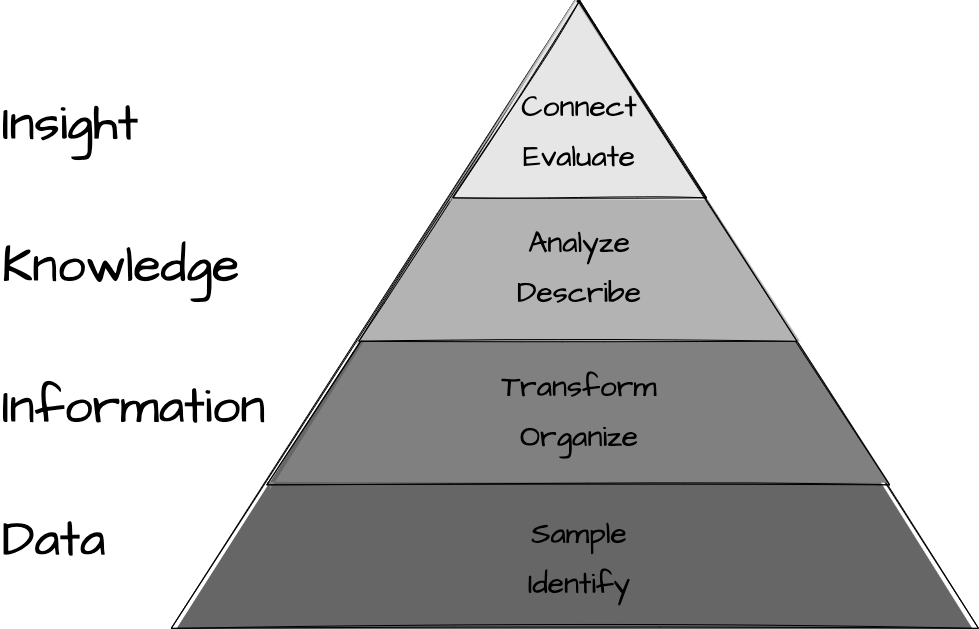
\includegraphics{part_0/figures/p-diki.drawio.png}}

}

\caption{\label{fig-diki-hierarchy}Data to Insight Hierarchy (DIKI)\\
Adapted from Ackoff (\citeproc{ref-Ackoff1989}{1989}) and Rowley
(\citeproc{ref-Rowley2007}{2007}).}

\end{figure}%

The DIKI Hierarchy highlights the stages and intermediate steps required
to derive insight from data. Part II ``Foundations'' provides a
conceptual introduction to the DIKI Hierarchy and establishes
foundational knowledge about data, information, knowledge, and insight
which is fundamental to developing a viable research plan.

Parts III ``Preparation'' and IV ``Analysis'' focus on the
implementation process. Part III covers the steps involved in preparing
data for analysis, including data acquisition, curation, and
transformation. Part IV covers the steps involved in conducting
analysis, including exploratory, predictive, and inferential data
analysis.

The final part, Part V ``Communication'', covers the final stage of the
data analysis process, which is to communicate the results of the
analysis. This includes the structure and content of research reports as
well as the process of publishing, sharing, and collaborating on
research.

\subsection*{Chapter level}\label{sec-preface-structure-chapter}
\addcontentsline{toc}{subsection}{Chapter level}

At the chapter level, both conceptual and programming skills are
developed in stages\footnote{These stages attempt to capture the general
  progression of learning reflected in Bloom's Taxonomy. See Krathwohl
  (\citeproc{ref-Krathwohl2002}{2002}) for a description and revised
  version.}. The chapter-level structure is consistent across chapters
and can be seen in Table~\ref{tbl-structure-approach}.

\begin{longtable}[]{@{}
  >{\raggedright\arraybackslash}p{(\columnwidth - 6\tabcolsep) * \real{0.1500}}
  >{\raggedright\arraybackslash}p{(\columnwidth - 6\tabcolsep) * \real{0.5500}}
  >{\raggedright\arraybackslash}p{(\columnwidth - 6\tabcolsep) * \real{0.1500}}
  >{\raggedright\arraybackslash}p{(\columnwidth - 6\tabcolsep) * \real{0.1500}}@{}}
\caption{The general structure and learning progression of a
chapter}\label{tbl-structure-approach}\tabularnewline
\toprule\noalign{}
\begin{minipage}[b]{\linewidth}\raggedright
Component
\end{minipage} & \begin{minipage}[b]{\linewidth}\raggedright
Purpose
\end{minipage} & \begin{minipage}[b]{\linewidth}\raggedright
Resource
\end{minipage} & \begin{minipage}[b]{\linewidth}\raggedright
Stage
\end{minipage} \\
\midrule\noalign{}
\endfirsthead
\toprule\noalign{}
\begin{minipage}[b]{\linewidth}\raggedright
Component
\end{minipage} & \begin{minipage}[b]{\linewidth}\raggedright
Purpose
\end{minipage} & \begin{minipage}[b]{\linewidth}\raggedright
Resource
\end{minipage} & \begin{minipage}[b]{\linewidth}\raggedright
Stage
\end{minipage} \\
\midrule\noalign{}
\endhead
\bottomrule\noalign{}
\endlastfoot
Outcomes & Identify the learning objectives for the chapter & Textbook &
Indicate \\
Overview & Provide a brief introduction to the chapter topic & Textbook
& Outline \\
Coding Lessons & Teach programming techniques with hands-on interactive
exercises & GitHub & Interact \\
Content & Combine conceptual discussions and programming skills,
incorporating thought-provoking questions, relevant studies, and
advanced topic references & Textbook & Explore \\
Recipes & Offer step-by-step programming examples related to the chapter
and relevant for the upcoming lab & Resources Kit website & Examine \\
Labs & Allow readers to apply chapter-specific concepts and techniques
to practical tasks & GitHub & Apply \\
Summary & Review the key concepts and skills covered in the chapter &
Textbook & Review \\
\end{longtable}

Each chapter will begin with a list of key learning outcomes followed by
a brief introduction to the chapter's content. The goal is to orient the
reader to the chapter. Next there will be a prompt to complete the
interactive coding lesson(s) to introduce readers to key programming
concepts related to the chapter though hands-on experience and then the
main content of the chapter will follow. The content will be a
combination of conceptual discussions and programming skills,
incorporating thought-provoking questions (`\faIcon{lightbulb} Consider
this'), relevant studies (`\faIcon{file-alt} Case study'), and advanced
topic references (`\faIcon{medal} Dive deeper'). Together these
components form the skills and knowledge phase.

The next phase is the application phase. This phase will include
step-by-step programming demonstrations related to the chapter (Recipes)
and lab exercises that allow readers to apply their knowledge and skills
chapter-related tasks. Finally, the chapters conclude with a summary of
the key concepts and skills covered in the chapter and in the associated
activites.

\section*{Resources}\label{sec-preface-resources}
\addcontentsline{toc}{section}{Resources}

\markright{Resources}

The description and location of the available resources to support the
aims and approach of this textbook appear in Table~\ref{tbl-resources}.

\begin{longtable}[]{@{}
  >{\raggedright\arraybackslash}p{(\columnwidth - 4\tabcolsep) * \real{0.1500}}
  >{\raggedright\arraybackslash}p{(\columnwidth - 4\tabcolsep) * \real{0.7000}}
  >{\raggedright\arraybackslash}p{(\columnwidth - 4\tabcolsep) * \real{0.1500}}@{}}
\caption{Resources available to support the aims and approach of this
textbook}\label{tbl-resources}\tabularnewline
\toprule\noalign{}
\begin{minipage}[b]{\linewidth}\raggedright
Resource
\end{minipage} & \begin{minipage}[b]{\linewidth}\raggedright
Description
\end{minipage} & \begin{minipage}[b]{\linewidth}\raggedright
Location
\end{minipage} \\
\midrule\noalign{}
\endfirsthead
\toprule\noalign{}
\begin{minipage}[b]{\linewidth}\raggedright
Resource
\end{minipage} & \begin{minipage}[b]{\linewidth}\raggedright
Description
\end{minipage} & \begin{minipage}[b]{\linewidth}\raggedright
Location
\end{minipage} \\
\midrule\noalign{}
\endhead
\bottomrule\noalign{}
\endlastfoot
Textbook & Prose discussion, figures/ tables, R code, case studies, and
thought and practical exercises & Physical/ GitHub \\
\{qtkit\} & R package with functions for accessing data and datasets, as
well as various useful functions developed specifically for this
textbook & CRAN/ GitHub \\
Resources Kit & Includes Recipes, programming tutorials to enhance the
reader's recognition of how programming strategies are implemented, and
other supplementary materials including setup Guides, and Instructor
materials & GitHub \\
Lessons & A set of interactive R programming lessons associated with
each chapter & GitHub \\
Labs & A set of lab exercises designed to direct the reader through
practical hands-on programming applications & GitHub \\
\end{longtable}

All resources are freely available and accessible to readers and are
found on the GitHub organization \url{https://github.com/qtalr/}. For
the textbook and Resources Kit, the code and a link to the website are
provided in each respective repository. The development version of the
\{qtkit\} package is available on GitHub and the stable version will be
available on CRAN. The interactive programming lessons and lab exercises
are also available on GitHub. Errata should be reported in the
respective repository's issue tracker on GitHub.

\section*{Getting started}\label{sec-preface-getting-started}
\addcontentsline{toc}{section}{Getting started}

\markright{Getting started}

Before jumping in to this and subsequent chapter's textbook activities,
it is important to prepare your computing environment and understand how
to take advantage of the resources available, both those directly and
indirectly associated with the textbook.

\subsection*{R and IDEs}\label{sec-preface-r-ides}
\addcontentsline{toc}{subsection}{R and IDEs}

Programming is the backbone for modern quantitative research. Among the
many programming languages available, R is a popular open-source
language and software environment for statistical computing. R is
popular with statisticians and has been adopted as the \emph{de facto}
language by many other fields in natural and social sciences, including
linguistics. It is freely downloadable from The R Project for
Statistical Programming website (\citeproc{ref-TheRFoundation2024}{The R
Foundation, 2024}) and is available for macOS, Linux, and Windows
operating systems.

Successfully installing R is rarely the last step in setting up your
R-enabled computing environment. The majority of R users also install an
\textbf{integrated development environment} (IDE). An IDE, such as
RStudio (\citeproc{ref-Posit2024}{Posit, 2024}), or a text editor, such
as Visual Studio Code (\citeproc{ref-Microsoft2024}{Microsoft, 2024}),
provide a \textbf{graphical user interface} (GUI) for working with R. In
effect, these interfaces provide a dashboard for working with R and are
designed to make it easier to write and execute R code. IDEs also
provide a number of other useful features such as syntax highlighting,
code completion, and debugging. IDEs are not required to work with R but
they are \emph{highly} recommended.

Choosing to install R and an IDE directly on your personal computer,
which is know as your \textbf{local environment}, is not the only option
to work with R. Other options include working with R in a \textbf{remote
environment} or a \textbf{virtual environment}.

\begin{tcolorbox}[enhanced jigsaw, left=2mm, toprule=.15mm, colback=white, colframe=quarto-callout-color-frame, arc=.35mm, rightrule=.15mm, bottomrule=.15mm, leftrule=.75mm, breakable, opacityback=0]

\textbf{\faIcon{file-code} Guides}

For more information and instructions on setting up an R environment for
using this book, consult the Resources Kit ``Setting up an R
environment'' guide.

\end{tcolorbox}

There are trade-offs in terms of cost, convenience, and flexibility when
choosing to work with R in a local, remote, or virtual environment. The
choice is yours and you can always change your mind later. The important
thing is to get started and begin learning R. Furthermore, any of the
approaches described here will be compatible with this textbook.

\subsection*{R packages}\label{sec-preface-r-packages}
\addcontentsline{toc}{subsection}{R packages}

As you progress in your R programming experience, you'll find yourself
leveraging code from other R users, which is typically provided as
packages. Packages are sets of functions and/ or datasets that are
freely accessible for download, designed to perform a specific set of
interrelated tasks. They enhance the capabilities of R. Official R
packages can be found in repositories like The Comprehensive R Archive
Network (CRAN) (\citeproc{ref-RCommunity2024}{R Community, 2024}) or
R-universe (\citeproc{ref-ROpenSci2024}{ROpenSci, 2024}), while other
packages can be obtained from code-sharing platforms such as GitHub
(\citeproc{ref-Github2024}{Github, 2024}).

\begin{tcolorbox}[enhanced jigsaw, left=2mm, toprule=.15mm, colback=white, colframe=quarto-callout-color-frame, arc=.35mm, rightrule=.15mm, bottomrule=.15mm, leftrule=.75mm, breakable, opacityback=0]

\textbf{\faIcon{lightbulb} Consider this}

The Comprehensive R Archive Network (CRAN) includes groupings of popular
packages related to a given applied programming task called Task Views
\url{https://cran.r-project.org/web/views/}. Explore the available CRAN
Task Views listings. Note the variety of areas (tasks) that are covered
in this listing. Now explore in more detail one of the following task
views which are directly related to topics covered in this textbook
noting the associated packages and their descriptions: (1) Cluster, (2)
MachineLearning, (3) NaturalLanguageProcessing, or (4)
ReproducibleResearch.

\end{tcolorbox}

You will download a number of packages at different stages of this
textbook, but there is a set of packages that will be key to have from
the get go. Once you have access to a working R/ RStudio environment,
you can proceed to install the following packages.

\begin{tcolorbox}[enhanced jigsaw, left=2mm, toprule=.15mm, colback=white, colframe=quarto-callout-color-frame, arc=.35mm, rightrule=.15mm, bottomrule=.15mm, leftrule=.75mm, breakable, opacityback=0]

\textbf{\faIcon{file-code} Guides}

For instructions on how to install the \{qtkit\} package from CRAN or
GitHub and download and use the interactive R programming lessons for
this textbook, see the Resources Kit ``Getting started'' guide.

\end{tcolorbox}

Install the following packages from CRAN.

\begin{itemize}
\tightlist
\item
  \{tidyverse\} (\citeproc{ref-R-tidyverse}{Wickham, 2023c})
\item
  \{pak\} (\citeproc{ref-R-pak}{Csárdi \& Hester, 2023})
\item
  \{tinytex\} (\citeproc{ref-R-tinytex}{Xie, 2023})
\item
  \{swirl\} (\citeproc{ref-R-swirl}{Kross, Carchedi, Bauer, \& Grdina,
  2020})
\end{itemize}

You can do this by running the following code in an R console:

\begin{Shaded}
\begin{Highlighting}[]
\CommentTok{\# install key packages from CRAN}
\FunctionTok{install.packages}\NormalTok{(}\FunctionTok{c}\NormalTok{(}\StringTok{"tidyverse"}\NormalTok{, }\StringTok{"pak"}\NormalTok{, }\StringTok{"tinytex"}\NormalTok{, }\StringTok{"swirl"}\NormalTok{))}
\end{Highlighting}
\end{Shaded}

\subsection*{Git and GitHub}\label{sec-preface-git-github}
\addcontentsline{toc}{subsection}{Git and GitHub}

\begin{tcolorbox}[enhanced jigsaw, left=2mm, toprule=.15mm, colback=white, colframe=quarto-callout-color-frame, arc=.35mm, rightrule=.15mm, bottomrule=.15mm, leftrule=.75mm, breakable, opacityback=0]

\textbf{\faIcon{file-code} Guides}

For more information and instructions on setting up version control and
interacting with GitHub consult the Resources Kit ``Setting up Git and
GitHub'' guide.

\end{tcolorbox}

GitHub is a code sharing website. Modern computing is highly
collaborative and GitHub is a very popular platform for sharing and
collaborating on coding projects. The lab exercises for this textbook
are shared on GitHub. To access and complete these exercises you will
need to sign up for a (free) GitHub account and then set up the version
control software \texttt{git} on your computing environment, if it is
not already.

\subsection*{Getting help}\label{sec-preface-getting-help}
\addcontentsline{toc}{subsection}{Getting help}

The technologies employed in this approach to text analysis will include
a somewhat steep learning curve. And in all honesty, the learning never
stops! Both seasoned programmers and beginners alike need assistance.
Fortunately there is a very large community of programmers who have
developed many official support resources and who actively contribute to
official and unofficial discussion forums. Together these resources
provide many avenues for overcoming challenges.

In Table~\ref{tbl-support-resources}, I provide a list of steps for
seeking help with R.

\begin{longtable}[]{@{}
  >{\raggedright\arraybackslash}p{(\columnwidth - 4\tabcolsep) * \real{0.0500}}
  >{\raggedright\arraybackslash}p{(\columnwidth - 4\tabcolsep) * \real{0.2500}}
  >{\raggedright\arraybackslash}p{(\columnwidth - 4\tabcolsep) * \real{0.7000}}@{}}
\caption{Recommended order for seeking help with
R}\label{tbl-support-resources}\tabularnewline
\toprule\noalign{}
\begin{minipage}[b]{\linewidth}\raggedright
Step
\end{minipage} & \begin{minipage}[b]{\linewidth}\raggedright
Resource
\end{minipage} & \begin{minipage}[b]{\linewidth}\raggedright
Description
\end{minipage} \\
\midrule\noalign{}
\endfirsthead
\toprule\noalign{}
\begin{minipage}[b]{\linewidth}\raggedright
Step
\end{minipage} & \begin{minipage}[b]{\linewidth}\raggedright
Resource
\end{minipage} & \begin{minipage}[b]{\linewidth}\raggedright
Description
\end{minipage} \\
\midrule\noalign{}
\endhead
\bottomrule\noalign{}
\endlastfoot
1 & Official R Documentation & Access the official documentation by
running \texttt{help(package\ =\ "package\_name")} in an R console. Use
the \texttt{?} operator followed by the package or function name. Check
out available Vignettes by running
\texttt{browseVignettes("package\_name")}. \\
2 & Web Search & Look for package documentation and vignettes on the
web. A popular site for this is R-Universe. \\
3 & RStudio IDE Help Toolbar & If you're using RStudio IDE, use the
``Help'' toolbar menu. It provides links to help resources, guides, and
manuals. \\
4 & Online Discussion Forums & Sites like Stack Overflow and RStudio
Community are great platforms where the programming community asks and
answers questions related to real-world issues. \\
5 & Post Questions with Reprex & When posting a question, especially
those involving coding issues or errors, provide enough background and
include a reproducible example (reprex) - a minimal piece of code that
demonstrates your issue. This helps others understand and answer your
question effectively. \\
\end{longtable}

\begin{tcolorbox}[enhanced jigsaw, left=2mm, toprule=.15mm, colback=white, colframe=quarto-callout-color-frame, arc=.35mm, rightrule=.15mm, bottomrule=.15mm, leftrule=.75mm, breakable, opacityback=0]

\textbf{\faIcon{file-code} Guides}

For information on how to create a minimal reproducible example with the
\{reprex\} package (\citeproc{ref-R-reprex}{Bryan, Hester, Robinson,
Wickham, \& Dervieux, 2024}), consult the Resources Kit ``Creating
reproducible examples'' guide.

\end{tcolorbox}

The take-home message here is that you are not alone. There are many
people world-wide that are learning to program and/ or contribute to the
learning of others. The more you engage with these resources and
communities the more successful your learning will be. As soon as you
are able, pay it forward. Posting questions and offering answers helps
the community and engages and refines your skills --a win-win.

\section*{Conventions}\label{sec-preface-conventions}
\addcontentsline{toc}{section}{Conventions}

\markright{Conventions}

To facilitate the learning process, this textbook will employ a number
of conventions. These conventions are intended to help the reader
navigate the text and to signal the reader's attention to important
concepts and information.

\subsection*{Prose}\label{sec-preface-prose}
\addcontentsline{toc}{subsection}{Prose}

The following typographic conventions are used throughout the text:

\begin{itemize}
\tightlist
\item
  \emph{Italics}

  \begin{itemize}
  \tightlist
  \item
    Filenames, file extensions, directory paths, and URLs.
  \end{itemize}
\item
  \texttt{Fixed-width}

  \begin{itemize}
  \tightlist
  \item
    Function names, variable and object names, and in-line code
    including expressions and operators.
  \end{itemize}
\item
  \{Curly brackets\}

  \begin{itemize}
  \tightlist
  \item
    R package names
  \end{itemize}
\item
  \textbf{Bold}

  \begin{itemize}
  \tightlist
  \item
    Key concepts when first introduced.
  \end{itemize}
\item
  \href{https://qtalr.github.io/qtkit/}{Linked text}

  \begin{itemize}
  \tightlist
  \item
    Links to internal and external resources, footnotes, and citations
    including references to R packages when first introduced.
  \end{itemize}
\end{itemize}

\subsection*{Code blocks}\label{sec-preface-code-blocks}
\addcontentsline{toc}{subsection}{Code blocks}

More lengthy code will be presented in code blocks, as seen in
Example~\ref{exm-code-block}.

\begin{example}[]\protect\hypertarget{exm-code-block}{}\label{exm-code-block}

~

\begin{Shaded}
\begin{Highlighting}[]
\CommentTok{\# A function that takes a name and returns a greeting}
\NormalTok{greetings }\OtherTok{\textless{}{-}} \ControlFlowTok{function}\NormalTok{(name) \{}
  \FunctionTok{paste}\NormalTok{(}\StringTok{"Hello"}\NormalTok{, name)}
\NormalTok{\}}

\FunctionTok{greetings}\NormalTok{(}\AttributeTok{name =} \StringTok{"Jerid"}\NormalTok{) }\CommentTok{\# apply function to a name}
\end{Highlighting}
\end{Shaded}

\begin{verbatim}
[1] "Hello Jerid"
\end{verbatim}

\end{example}

There are a couple of things to note about the code in
Example~\ref{exm-code-block}. First, it shows the code that is run in R
as well as the ouput that is returned. The code will appear in a box and
the output will appear below the box. Both code and output will appear
in fixed-width font. Second, the \texttt{\#} symbol within a code block
is used to signal a \textbf{code comment}, a human-facing description.
Everything right of a \texttt{\#} is not run as code. In this textbook
you will see code comments above code on a separate line and/ or to the
right of code on the same line. It is good practice to comment your code
to enhance readability and to help others understand what your code is
doing.

All figures, tables, and images in this textbook are generated by code
blocks but only code for those elements that are relevant for discussion
will be shown. However, if you wish to see the code for any element in
this textbook, you can visit the GitHub repository
\url{https://qtalr.github.io/book/}.

When a reference to a snippet of a file, it will appear as in
Snippet~\ref{lst-r-code}.

\begin{codelisting}

\caption{\label{lst-r-code}\emph{example.R} file}

\centering{

\begin{Shaded}
\begin{Highlighting}[]
\CommentTok{\# Load package}
\FunctionTok{library}\NormalTok{(tidyverse)}

\CommentTok{\# Add 1 and 1}
\DecValTok{1} \SpecialCharTok{+} \DecValTok{1}
\end{Highlighting}
\end{Shaded}

}

\end{codelisting}%

\subsection*{Callouts}\label{sec-preface-callouts}
\addcontentsline{toc}{subsection}{Callouts}

Callouts are used to signal the reader's attention to content, activity,
and other important sections. The following callouts are used in this
textbook:

\textbf{Content}

\begin{tcolorbox}[enhanced jigsaw, left=2mm, toprule=.15mm, colback=white, colframe=quarto-callout-color-frame, arc=.35mm, rightrule=.15mm, bottomrule=.15mm, leftrule=.75mm, breakable, opacityback=0]

\textbf{\faIcon{list-alt} Outcomes}

Learning outcomes for the chapter.

\end{tcolorbox}

\begin{tcolorbox}[enhanced jigsaw, left=2mm, toprule=.15mm, colback=white, colframe=quarto-callout-color-frame, arc=.35mm, rightrule=.15mm, bottomrule=.15mm, leftrule=.75mm, breakable, opacityback=0]

\textbf{\faIcon{lightbulb} Consider this}

Points to consider and questions to explore.

\end{tcolorbox}

\begin{tcolorbox}[enhanced jigsaw, left=2mm, toprule=.15mm, colback=white, colframe=quarto-callout-color-frame, arc=.35mm, rightrule=.15mm, bottomrule=.15mm, leftrule=.75mm, breakable, opacityback=0]

\textbf{\faIcon{file-alt} Case study}

Case studies which highlight conceptual knowledge and coding skills.

\end{tcolorbox}

\begin{tcolorbox}[enhanced jigsaw, left=2mm, toprule=.15mm, colback=white, colframe=quarto-callout-color-frame, arc=.35mm, rightrule=.15mm, bottomrule=.15mm, leftrule=.75mm, breakable, opacityback=0]

\textbf{\faIcon{medal} Dive deeper}

Additional comments and resources for diving deeper into a topic.

\end{tcolorbox}

\textbf{Activities}

\begin{tcolorbox}[enhanced jigsaw, left=2mm, toprule=.15mm, colback=white, colframe=quarto-callout-color-frame, arc=.35mm, rightrule=.15mm, bottomrule=.15mm, leftrule=.75mm, breakable, opacityback=0]

\textbf{\faIcon{terminal} Lessons}

Links to interactive lessons for practicing coding skills.

\end{tcolorbox}

\begin{tcolorbox}[enhanced jigsaw, left=2mm, toprule=.15mm, colback=white, colframe=quarto-callout-color-frame, arc=.35mm, rightrule=.15mm, bottomrule=.15mm, leftrule=.75mm, breakable, opacityback=0]

\textbf{\faIcon{file-code} Recipe}

Reading to examine programming concepts.

\end{tcolorbox}

\begin{tcolorbox}[enhanced jigsaw, left=2mm, toprule=.15mm, colback=white, colframe=quarto-callout-color-frame, arc=.35mm, rightrule=.15mm, bottomrule=.15mm, leftrule=.75mm, breakable, opacityback=0]

\textbf{\faIcon{flask} Lab}

Exercises for applying conceptual knowledge and coding skills.

\end{tcolorbox}

\textbf{Other}

\begin{tcolorbox}[enhanced jigsaw, left=2mm, toprule=.15mm, colback=white, colframe=quarto-callout-color-frame, arc=.35mm, rightrule=.15mm, bottomrule=.15mm, leftrule=.75mm, breakable, opacityback=0]

\textbf{\faIcon{hand-point-up} Tip}

Tips for using R and related tools.

\end{tcolorbox}

\begin{tcolorbox}[enhanced jigsaw, left=2mm, toprule=.15mm, colback=white, colframe=quarto-callout-color-frame, arc=.35mm, rightrule=.15mm, bottomrule=.15mm, leftrule=.75mm, breakable, opacityback=0]

\textbf{\faIcon{exclamation-triangle} Warning}

Warnings for using R and related tools.

\end{tcolorbox}

\section*{Activities}\label{sec-preface-activities}
\addcontentsline{toc}{section}{Activities}

\markright{Activities}

At this point you should have a working R environment with the core
packages including \{qtkit\} installed. You should also have verified
that you have a working Git environment and that you have a GitHub
account. If you have not completed these tasks, return to the guides
listed above in ``\hyperref[sec-preface-getting-started]{Getting
started}'' of this Preface and complete them before proceeding.

The following activities are designed to help you become familiar with
the tools and resources that you will be using throughout this textbook.
These and subsequent activities are designed to be completed in the
order that they are presented in this textbook.

\begin{tcolorbox}[enhanced jigsaw, left=2mm, toprule=.15mm, colback=white, colframe=quarto-callout-color-frame, arc=.35mm, rightrule=.15mm, bottomrule=.15mm, leftrule=.75mm, breakable, opacityback=0]

\textbf{\faIcon{terminal} Lessons}

\textbf{What}: Intro to Swirl\\
\textbf{How}: In the R console load \{swirl\}, run \texttt{swirl()}, and
follow prompts to select the lesson.\\
\textbf{Why}: To familiarize you with navigating, selecting, and
completing swirl lessons for interactive R programming tutorials.

\end{tcolorbox}

\begin{tcolorbox}[enhanced jigsaw, left=2mm, toprule=.15mm, colback=white, colframe=quarto-callout-color-frame, arc=.35mm, rightrule=.15mm, bottomrule=.15mm, leftrule=.75mm, breakable, opacityback=0]

\textbf{\faIcon{file-code} Recipe}

\textbf{What}: Literate Programming and Quarto\\
\textbf{How}: Read Recipe 0, complete comprehension check, and prepare
for Lab 0.\\
\textbf{Why}: To introduce the concept of Literate Programming and how
to create literate documents using R and Quarto.

\end{tcolorbox}

\begin{tcolorbox}[enhanced jigsaw, left=2mm, toprule=.15mm, colback=white, colframe=quarto-callout-color-frame, arc=.35mm, rightrule=.15mm, bottomrule=.15mm, leftrule=.75mm, breakable, opacityback=0]

\textbf{\faIcon{flask} Lab}

\textbf{What}: Writing with code\\
\textbf{How}: Clone, fork, and complete the steps in Lab 0.\\
\textbf{Why}: To put literate programming techniques covered in Recipe 0
into practice. Specifically, you will create and edit a Quarto document
and render a report in PDF format.

\end{tcolorbox}

\section*{Summary}\label{sec-preface-summary}
\addcontentsline{toc}{section}{Summary}

\markright{Summary}

This prefaces outlines the textbook's underlying principles, learning
goals, teaching methods, and target audience. The chapter also offers
advice on how to navigate the book's layout, comprehend its subject
matter, and make use of supplementary materials. With this foundation,
you're now prepared to dig into quantitative text analysis. I hope you
enjoy the journey!

\section*{To the instructor}\label{sec-preface-instructor}
\addcontentsline{toc}{section}{To the instructor}

\markright{To the instructor}

For recommendations on how to use this textbook in your course and to
access additional resources, visit the Resources Kit ``Instructor
Guide''. The guide provides information on how to structure your course,
how to use the textbook, and how to access additional resources to
support your teaching.

\part{Orientation}

In this introductory part, we explore fundamentatl concepts that are
essential for understanding text analysis in its research and
methodological context. We start by pointing to the limitations of human
cognition in processing vast amounts of information and that underscore
the need for scientific methods to objectively analyze data. A brief
history of quantitative data analysis highlights the commonalities
between text analysis and other quantitative methods. We then discuss
the role of quantitative methods in language research, and how text
analysis contributes to the field.

\chapter{Text analysis}\label{sec-text-chapter}

\begin{quote}
Everything about science is changing because of the impact of
information technology and the data deluge.

--- Jim Gray
\end{quote}

\begin{tcolorbox}[enhanced jigsaw, left=2mm, toprule=.15mm, colback=white, colframe=quarto-callout-color-frame, arc=.35mm, rightrule=.15mm, bottomrule=.15mm, leftrule=.75mm, breakable, opacityback=0]

\textbf{\faIcon{list-alt} Outcomes}

\begin{itemize}
\tightlist
\item
  Understand the role and goals of data analysis both within and outside
  of academia.
\item
  Describe the various approaches to quantitative language research.
\item
  Identify the applications of text analysis in different contexts.
\end{itemize}

\end{tcolorbox}

In this chapter, I introduce the topic of text analysis and provide the
context needed to understand how it fits in a larger universe of science
and the ever-ubiquitous methods of data science. Approaches to language
analysis, including methodological approaches and the nature of data,
are discussed. I then introduce text analysis as a branch of data
science and discuss its aims, approaches, implementation, and
applications.

\begin{tcolorbox}[enhanced jigsaw, left=2mm, toprule=.15mm, colback=white, colframe=quarto-callout-color-frame, arc=.35mm, rightrule=.15mm, bottomrule=.15mm, leftrule=.75mm, breakable, opacityback=0]

\textbf{\faIcon{terminal} Lessons}

\textbf{What}: Workspace, Vectors\\
\textbf{How}: In an R console load \{swirl\}, run \texttt{swirl()}, and
follow prompts to select the lesson.\\
\textbf{Why}: To examine your local workspace in RStudio and understand
the relationship between your R workspace and the file system of your
computing environment. To explore the key building blocks of the R
programming language.

\end{tcolorbox}

\section{Enter science}\label{sec-enter-science}

The world around us is full of countless actions and interactions. As
individuals, we experience this world, gaining knowledge and building
heuristic understanding of how it works. Our minds process countless
sensory inputs, which enable skills and abilities that we often take for
granted, such as predicting what will happen if someone is about to
knock a wine glass off a table and onto a concrete floor. Even if we
have never encountered this specific situation before, our minds somehow
instinctively make an effort to warn the potential glass-breaker before
it is too late.

You may have attributed this predictive knowledge to `common sense'.
Despite its commonality, it is an incredible display of the brain's
capacity to monitor the environment, make connections, and store
information without consciously informing us about its processes.

Our brains are efficient but not infallible. They do not store every
experience in raw form; we don't have access to records like a computer
would. Instead, our brains excel in making associations and predictions
that help us navigate the complex world we inhabit. In addition, our
brains are prone to biases that can influence our understanding of the
world. For example, confirmation bias leads us to seek out information
that confirms our beliefs, while the availability heuristic causes us to
overestimate the likelihood of easily recalled events.

our brains are doing some amazing work, but that work can give us the
impression that we understand the world better and in more detail than
we actually do. In this way, what we think the world is like and what
the world is actually like can be two different things. This is
problematic for making sense of the world in an objective way. This is
where science comes in.

\begin{tcolorbox}[enhanced jigsaw, left=2mm, toprule=.15mm, colback=white, colframe=quarto-callout-color-frame, arc=.35mm, rightrule=.15mm, bottomrule=.15mm, leftrule=.75mm, breakable, opacityback=0]

\textbf{\faIcon{lightbulb} Consider this}

How might your own experiences and biases influence your understanding
of the world? What are some ways that you can mitigate these biases? Is
ever possible to be completely objective? How might biases influence the
way you approach text analysis?

\end{tcolorbox}

Science starts with a question, identifies and collects data, careful
selected slices of the complex world, submits this data to analysis
through clearly defined and reproducible procedures, and reports the
results for others to evaluate. This process is repeated, modifying, and
manipulating the procedures, asking new questions and positing new
explanations, all in an effort to make inroads to bring the complex into
tangible view.

In essence what science does is attempt to subvert our inherent
limitations by drawing on carefully and purposefully collected samples
of observable experience and letting the analysis of these observations
speak, even if it goes against our intuitions (those powerful but
sometime spurious heuristics that our brains use to make sense of the
world).

\section{Data analysis}\label{data-analysis}

\subsection{Emergence of data science}\label{emergence-of-data-science}

This science I've described is the one you are likely quite familiar
with and, if you are like me, this description of science conjure
visions of white coats, labs, and petri dishes. While science's
foundation still stands strong in the 21st century, a series of
intellectual and technological events mid-20th century set in motion
changes that have changed aspects about how science is done, not why it
is done. We could call this Science 2.0, but let's use the more
popularized term \index{data science}\textbf{data science}.

The recognized beginnings of data science are attributed to work in the
``Statistics and Data Analysis Research'' department at Bell Labs during
the 1960s. Although primarily conceptual and theoretic at the time, a
framework for quantitative data analysis took shape that would
anticipate what would come: sizable datasets which would ``{[}\ldots{]}
require advanced statistical and computational techniques {[}\ldots{]}
and the software to implement them.''
(\citeproc{ref-Chambers2020}{Chambers, 2020}) This framework emphasized
both the inference-based research of traditional science, but also
embraced exploratory research and recognized the need to address
practical considerations that would arise when working with and deriving
insight from an abundance of machine-readable data.

Fast-forward to the 21st century, a world in which machine-readable data
is truly in abundance. With increased computing power, the emergence of
the world wide web, and wide adoption of mobile devices electronic
communication skyrocketed around the globe. To put this in perspective,
in 2019 it was estimated that every minute 511 thousand tweets were
posted, 18.1 million text messages were sent, and 188 million emails
were sent (\citeproc{ref-DataNeverSleeps08-2021}{{``Data never sleeps
7.0 infographic,''} 2019}). The data flood has not been limited to
language, there are more sensors and recording devices than ever before
which capture evermore swaths of the world we live in
(\citeproc{ref-Desjardins2019}{Desjardins, 2019}).

Where increased computing power gave rise to the influx of data, it is
also one of the primary methods for gathering, preparing, transforming,
analyzing, and communicating insight derived from this data
(\citeproc{ref-Donoho2017}{Donoho, 2017}). The vision laid out in the
1960s at Bell Labs had come to fruition.

\subsection{Data science toolbelt}\label{data-science-toolbelt}

Data science is not predicated on data alone. Turning data into insight
takes computing skills, statistical knowledge, and domain expertise.
This triad has been popularly represented as a Venn diagram such as in
Figure~\ref{fig-intro-data-science-venn}.

\begin{figure}[t]

\centering{

{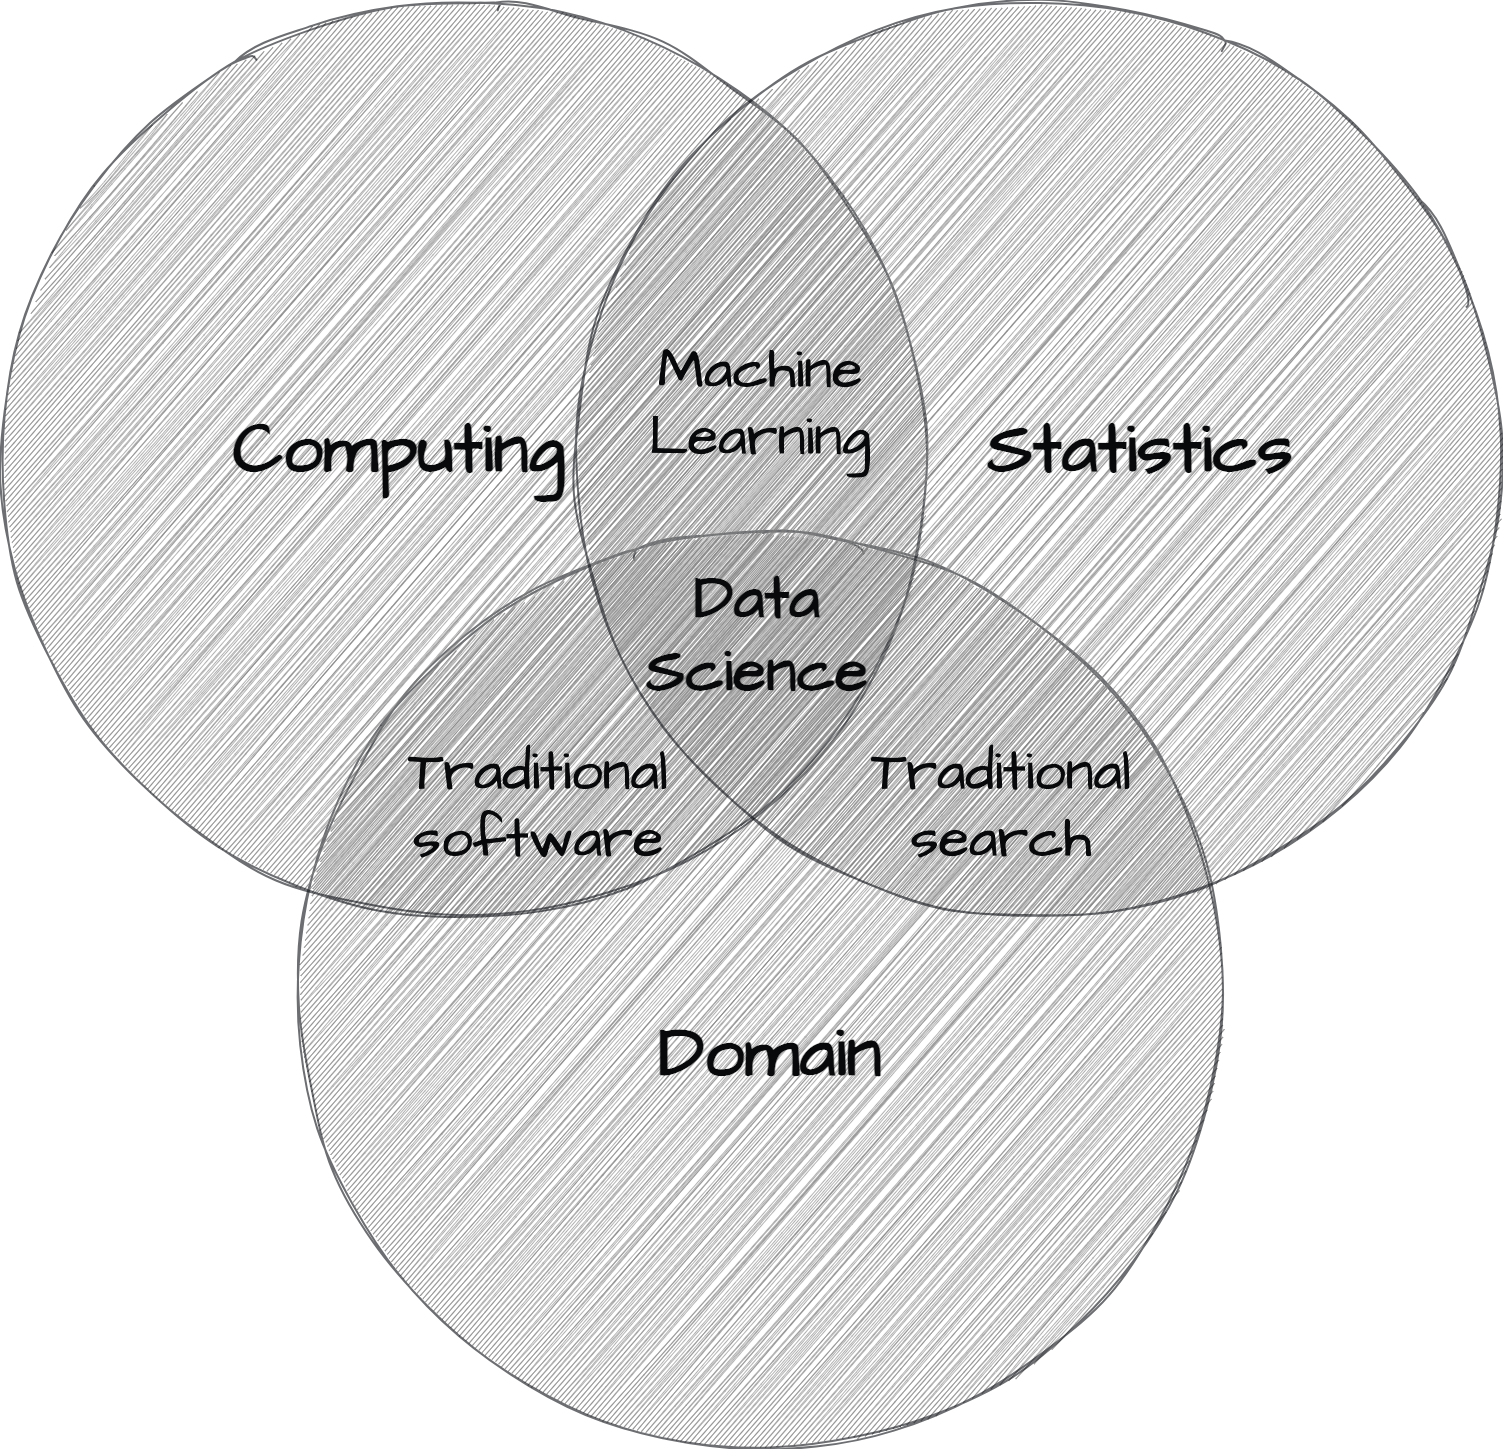
\includegraphics[width=0.6\textwidth,height=\textheight]{part_1/figures/text-ds-venn.drawio.png}}

}

\caption{\label{fig-intro-data-science-venn}Data Science Venn Diagram
adapted from D. Conway (\citeproc{ref-Conway2010}{2010}).}

\end{figure}%

The \index{computing skills}\textbf{computing skills} component of data
science is the ability to write code to perform the data analysis
process. This is the primary approach for working with data at scale.
The \index{statistical knowledge}\textbf{statistical knowledge}
component of data science is the ability to apply statistical methods to
data to derive insight by bringing patterns and relationships in the
data into view. \index{Domain expertise}\textbf{Domain expertise}
provides researchers insight at key junctures in the development of a
research project and aid researchers in evaluating results.

This triad of skills in combination with reproducible research practices
is the foundational toolbelt of data science
(\citeproc{ref-Hicks2019}{Hicks \& Peng, 2019}). \textbf{Reproducible
research}\index{reproducible research} entails the use of computational
tools to automate the process of data analysis. This automation is
achieved by writing code that can be executed to replicate the data
analysis. This code can then be shared through code sharing
repositories, where it can be viewed, downloaded, and executed by
others. This adds transparency to the process and allows others to build
on previous work enhacing scientific progress along the way
(\citeproc{ref-Baker2016}{Baker, 2016}).

\subsection{Quant everywhere}\label{quant-everywhere}

Equipped with the data science toolbelt, the interest in deriving
insight from data is now almost ubiquitous. The science of data has now
reached deep into all aspects of life where making sense of the world is
sought. Predicting whether a loan applicant will get a loan
(\citeproc{ref-Bao2019}{Bao, Lianju, \& Yue, 2019}), whether a lump is
cancerous (\citeproc{ref-Saxena2020}{Saxena \& Gyanchandani, 2020}),
what films to recommend based on your previous viewing history
(\citeproc{ref-Gomez-Uribe2015}{Gomez-Uribe \& Hunt, 2015}), what
players a sports team should sign (\citeproc{ref-Lewis2004}{Lewis,
2004}), now all incorporate a common set of data analysis tools.

The data science toolbelt also underlies well-known public-facing
language applications. From the language-capable chat applications,
plagiarism detection software, machine translation algorithms, and
search engines, tangible results of quantitative approaches to language
are becoming standard fixtures in our lives.

The spread of quantitative data analysis too has taken root in academia.
Even in areas that on first blush don't appear readily approachable in a
quantitative manner, such as fields in the social sciences and
humanities, data science is making important and sometimes disciplinary
changes to the way that academic research is conducted.

This textbook focuses in on a domain that cuts across many of these
fields; namely language. At this point let's turn to quantitative
approaches to language analysis as we work closer to contextualizing
text analysis in the field of linguistics.

\section{Language analysis}\label{language-analysis}

\subsection{Qualities and quantities}\label{qualities-and-quantities}

Language is a defining characteristic of our species. Since antiquity,
language has attracted interest across disciplines and schools of
thought. In the early 20th century, the development of the rigorous
approach to study of language as a field in its own right took root
(\citeproc{ref-Campbell2001}{Campbell, 2001}), yet a plurality of
theoretical views and methodological approaches remained. Contemporary
linguistics bares this complex history and even today, it is far from
theoretically and methodologically unified discipline.

Either based on the tenets of theoretical frameworks and/ or the objects
of study of particular fields, methodological approaches to language
research vary. On the one hand, some language research commonly applies
qualitative assessment of language structure and/ or use.
\textbf{Qualitative approaches} describe and account for
characteristics, or ``qualities'', that can be observed, but not
measured (\emph{e.g.} introspective methods, ethnographic methods,
\emph{etc.})

On the other hand, other language research programs employ quantitative
research methods either out of necessity given the object of study
(phonetics, psycholinguistics, \emph{etc.}) or based on theoretical
principles (Cognitive Linguistics, Connectionism, \emph{etc.}).
\textbf{Quantitative approaches} involve ``quantities'' of properties
that can be observed and measured (\emph{e.g.} frequency of use,
reaction time, \emph{etc.}).

\begin{tcolorbox}[enhanced jigsaw, left=2mm, toprule=.15mm, colback=white, colframe=quarto-callout-color-frame, arc=.35mm, rightrule=.15mm, bottomrule=.15mm, leftrule=.75mm, breakable, opacityback=0]

\textbf{\faIcon{file-alt} Case study}

Manning (\citeproc{ref-Manning2003}{2003}) discusses the use of
probabilistic models in syntax to account for the variability in
language usage and the presence of both hard and soft constraints in
grammar. The paper touches on the statistical methods in text analysis,
the importance of distinguishing between external and internal language,
and the limitations of Generative Grammar. Overall, the paper suggests
that usage-based and formal syntax can learn from each other to better
understand language variation and change.

\end{tcolorbox}

These latter research areas and theoretical paradigms employ methods
that share much of the common data analysis toolbox described in the
previous section. In effect, this establishes a common methodological
language between other language-based research fields but also with
research outside of linguistics.

\subsection{The nature of data}\label{the-nature-of-data}

In quantitative language analysis, there is a key methodological
distinction between experimental and observational data, which affects
both procedure and interpretation of research.

\textbf{Experimental approaches} start with a intentionally designed
hypothesis and lay out a research methodology with appropriate
instruments and a plan to collect data that shows promise for shedding
light on the likelihood of the hypothesis. Experimental approaches are
conducted under controlled contexts, usually a lab environment, in which
participants are recruited to perform a language related task with
stimuli that have been carefully curated by researchers to elicit some
aspect of language behavior of interest. Experimental approaches to
language research are heavily influenced by procedures adapted from
psychology.

\textbf{Observational approaches} are a bit more of a mixed bag in terms
of the rationale for the study; they may either start with a testable
hypothesis or in other cases may start with a more open-ended research
question to explore. But a more fundamental distinction between the two
approaches is drawn in the amount of control the researcher exerts on
the contexts and conditions in which the language behavior data to be
collected is produced. Observational approaches seek out records of
language behavior that is produced by language speakers for
communicative purposes in natural(-istic) contexts. This may take place
in labs (language development, language disorders, \emph{etc.}), but
more often than not, language is collected from sources where speakers
are performing language as part of their daily lives --whether that be
posting on social media, speaking on the telephone, making political
speeches, writing class essays, reporting the latest news for a
newspaper, or crafting the next novel destined to be a New York Times
best-seller.

The data acquired from either of these approaches have their trade-offs.
The directness and level of control of experimental approaches has the
benefit of allowing researchers to precisely track how particular
experimental conditions effect language behavior. As these conditions
are an explicit part of the design, the resulting language behavior can
be more precisely attributed to the experimental manipulation.

The primary shortcoming of experimental approaches is that there is a
level of artificialness to this directness and control. Whether it is
the language materials used in the task, the task itself, or the fact
that the procedure takes place under supervision the language behavior
elicited can diverge quite significantly from language behavior
performed in natural communicative settings.

Observational approaches show complementary strengths and shortcomings.
Whereas experimental approaches may diverge from natural language use,
observational approaches strive to identify and collected language
behavior data in natural, uncontrolled, and unmonitored contexts. This
has the benefit of providing a more ecologically valid representation of
language behavior.

However, the contexts in which natural language communication take place
are complex relative to experimental contexts. Language collected from
natural contexts are nested within the complex workings of a complex
world and as such inevitably include a host of factors and conditions
which can prove challenging to disentangle from the language phenomenon
of interest but must be addressed in order to draw reliable associations
and conclusions.

\begin{figure}[!htb]

\centering{

{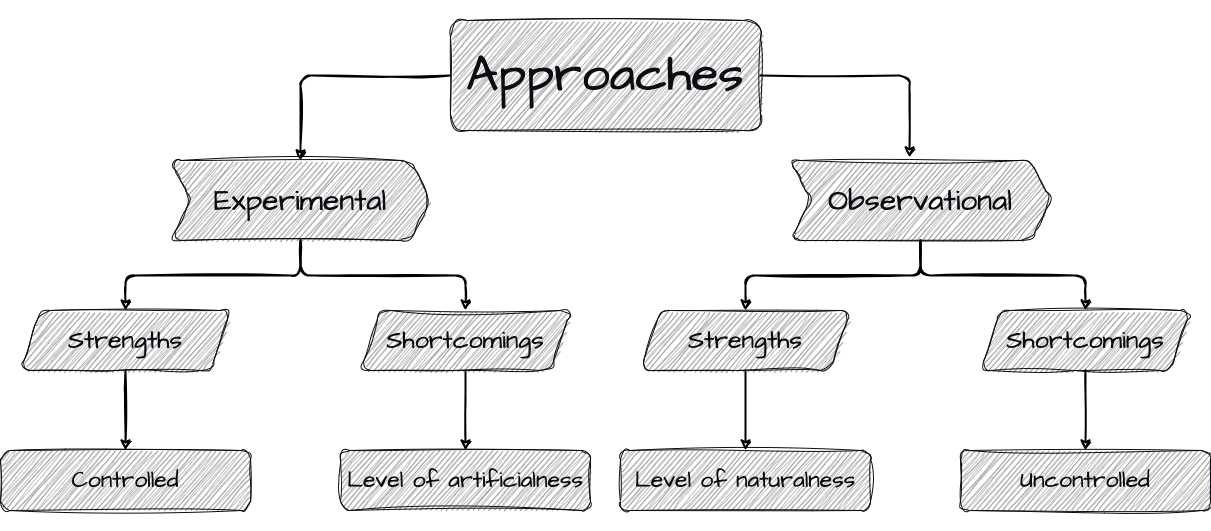
\includegraphics{part_1/figures/text-data-collection-methods.drawio.png}}

}

\caption{\label{fig-data-collection-methods}Trade-offs between
experimental and observational data collection methods}

\end{figure}%

The upshot, then, is two-fold: (1) data collection methods matter for
research design and interpretation and (2) there is no single best
approach to data collection, each have their strengths and shortcomings.

Ideally, a robust science of language will include insight from both
experimental and observational approaches
(\citeproc{ref-Gilquin2009}{Gilquin \& Gries, 2009}). And evermore there
is greater appreciation for the complementary nature of experimental and
observational approaches and a growing body of research which highlights
this recognition.

\section{Text analysis}\label{text-analysis}

In a nutshell, \textbf{text analysis}\index{Text analysis} is the
process of leveraging the data science toolbelt to derive insight from
textual data collected through observational methods. In the next
subsections, I will unpack this definition and discuss the primary
components that make up text analysis including research appoaches and
technical implementation, as well as practical applications.

\subsection{Aims}\label{aims}

Text analysis is a multifacited research methodology. It can be used use
facilitate the qualitative exploration of smaller, human-digestable
textual information, but is more often employed quantitatively to bring
to the surface patterns and relationships in large samples of textual
data that would be otherwise difficult, if not impossible, to identify
manually.

The aims of text analysis are as varied as the research questions that
can be asked of language data. Some research questions are data-driven,
where the researcher is interested in exploring and uncovering patterns
and relationships in the data. Other research questions are
theory-driven, where the researcher is interested in testing a
hypothesis or evaluating a theory. In either case, the researcher is
interested in gaining insight from the data.

The relationship(s) of interest in text analysis may be language
internal, where the researcher is interested in the patterns and
relationships between linguistic features or language external, where
the researcher is interested in the patterns and relationships between
linguistic features and some external variable.

\subsection{Implementation}\label{implementation}

Text analysis is branch of data science. As such, it takes advantage of
the data science toolbelt to derive insight from data. It is important
to note, that while all of the components of the data science toolbelt
are present in text analysis, the relative importance of each varies
with the stage research. Computing skills being the most important at
the data and information stages, statistical knowledge being the most
important to derive knowledge, and domain knowledge leading the way
towards insight.

Text is a rather raw form of data. It is more often that not
unstructured, meaning that it is not organized in a way that such that
it can be easily analyzed. The collection, organization, and
transformation of text data is a key component of text analysis and
computers are well-suited for this task, as we will see in
Chapter~\ref{sec-data-chapter} and Part III ``Preparation''.

Once text is transformed to a dataset that can be analyzed, we lean on
statistical methods to gain perspective on the relationship(s) of
interest. By and large, these methods are the same as those used in
other areas of data science. We will provide an overview of these
methods in Chapter~\ref{sec-analysis-chapter} and do a deeper dive in
Part IV ``Analysis''.

With the results of the analysis in hand, the researcher must interpret
the results and evaluate their significance in disciplinary context.
This is where domain knowledge comes to the fore. The researcher must be
able to interpret the results in light of the research question and the
context in which the data was collected and communicate the value of the
results to the broader community. Domain knowledge also plays a vital
role in framing the research question and designing the research
methodology, as we will see in Chapter~\ref{sec-research-chapter}. Then
we will return to the role of domain knowledge in interpreting and
communicating the results in Part V ``Communication''.

To ensure that the results of text analysis projects are replicable and
transparent, programming strategies and documentation play an integral
role at each stage of the implementation of a research project. While
there are a number of programming languages that can be used for text
analysis, R widely adopted in linguistics research and is the language
of choice for this textbook. R, in combination with literate programming
and other tools, provides a robust and reproducible workflow for text
analysis projects.

\subsection{Applications}\label{applications}

So what are some applications of text analysis? Most public facing
applications stem from Computational Linguistic research, often known as
\textbf{Natural Language Processing} (NLP) by practitioners. Whether it
be using search engines, online translators, submitting your paper to
plagiarism detection software, \emph{etc.} many of the text analysis
methods we will cover are at play.

\begin{tcolorbox}[enhanced jigsaw, left=2mm, toprule=.15mm, colback=white, colframe=quarto-callout-color-frame, arc=.35mm, rightrule=.15mm, bottomrule=.15mm, leftrule=.75mm, breakable, opacityback=0]

\textbf{\faIcon{lightbulb} Consider this}

What are some other public facing applications of text analysis that you
are aware of? Consider examples from social media, news, entertainment,
or other areas of interest. You may also consider how text analysis is
used in academia, if you are familiar with any examples.

\end{tcolorbox}

In academia, the use of quantitative text analysis is even more
widespread, despite the lack of public fanfare. In linguistics, text
analysis research is often falls under
\index{corpus linguistics}\textbf{Corpus Linguistics} (CL). And this
approach is applied to a wide range of topics and research questions in
both theoretical and applied linguistics fields and subfields, as seen
in Example~\ref{exm-linguistic-theory} and
Example~\ref{exm-linguistic-applied}.

\begin{example}[]\protect\hypertarget{exm-linguistic-theory}{}\label{exm-linguistic-theory}

Theoretical linguistics

\begin{itemize}
\tightlist
\item
  Hay (\citeproc{ref-Hay2002}{2002}) use a corpus study to investigate
  the role of frequency and phonotatics in affix ordering in English.
\item
  Riehemann (\citeproc{ref-Riehemann2001}{2001}) explores the extent to
  which idiomatic expressions (\emph{e.g.} `raise hell') are lexical or
  syntactic units.
\item
  Bresnan (\citeproc{ref-Bresnan2007a}{2007}) investigate the claim that
  possessed deverbal nouns in English (\emph{e.g.} `the city's
  destruction') are subject to a syntactic constraint that requires the
  possessor to be affected by the action denoted by the deverbal noun.
\end{itemize}

\end{example}

\begin{example}[]\protect\hypertarget{exm-linguistic-applied}{}\label{exm-linguistic-applied}

Applied linguistics

\begin{itemize}
\tightlist
\item
  Wulff, Stefanowitsch, \& Gries (\citeproc{ref-Wulff2007}{2007})
  explore differences between British and American English at the
  lexico-syntactic level in the \emph{into}-causative construction
  (\emph{e.g.} `He tricked me into employing him.').
\item
  Eisenstein, O'Connor, Smith, \& Xing
  (\citeproc{ref-Eisenstein2012}{2012}) track the geographic spread of
  neologisms (\emph{e.g.} `bruh', `af', '-\_\_-') from city to city in
  the United States using Twitter data collected between 6/2009 and
  5/2011.
\item
  Bychkovska \& Lee (\citeproc{ref-Bychkovska2017}{2017}) investigates
  possible differences between L1-English and L1-Chinese undergraduate
  students' use of lexical bundles, multiword sequences which are
  extended collocations (\emph{e.g.} `as the result of'), in
  argumentative essays.
\item
  Jaeger \& Snider (\citeproc{ref-Jaeger2007}{2007}) use a corpus study
  to investigate the phenomenon of syntactic persistence, the increased
  tendency for speakers to use a particular syntactic form over an
  alternate when the syntactic form has been recently processed.
\item
  Voigt et al. (\citeproc{ref-Voigt2017}{2017}) explore potential racial
  disparities in officer respect in police body camera footage.
\item
  Olohan (\citeproc{ref-Olohan2008}{2008}) investigate the extent to
  which translated texts differ from native texts do to `explicitation'.
\end{itemize}

\end{example}

So too, text analysis is used in a variety of fields outside of
linguistics where insight from language is sought, as seen in
Example~\ref{exm-other-fields}.

\begin{example}[]\protect\hypertarget{exm-other-fields}{}\label{exm-other-fields}

Language-related fields

\begin{itemize}
\tightlist
\item
  Kloumann, Danforth, Harris, \& Bliss
  (\citeproc{ref-Kloumann2012}{2012}) explore the extent to which
  languages are positively, neutrally, or negatively biased.
\item
  Mosteller \& Wallace (\citeproc{ref-Mosteller1963}{1963}) provide a
  method for solving the authorship debate surrounding The Federalist
  papers.
\item
  L. G. Conway et al. (\citeproc{ref-Conway2012}{2012}) investigate
  whether the established drop in language complexity of rhetoric in
  election seasons is associated with election outcomes.
\end{itemize}

\end{example}

\begin{tcolorbox}[enhanced jigsaw, left=2mm, toprule=.15mm, colback=white, colframe=quarto-callout-color-frame, arc=.35mm, rightrule=.15mm, bottomrule=.15mm, leftrule=.75mm, breakable, opacityback=0]

\textbf{\faIcon{lightbulb} Consider this}

Language is a key component of human communication and interaction. What
are some other areas of research in and outside linguistics that you
think could be explored using text analysis methods?

\end{tcolorbox}

These studies in Examples \ref{exm-linguistic-theory},
\ref{exm-linguistic-applied}, and \ref{exm-other-fields} are just a few
illustrations of the contributions of text analysis used as the primary
method to gain a deeper understanding of language structure, function,
variation, and acquisition.

As a method, however, text analysis can also be used to support other
research methods. For example, text analysis can be used collect data,
generate authentic materials, provide linguistic annotation, and to
generate hypotheses, for either qualitative or quantitative approaches.
Together these efforts contribute to a more robust language science by
incorporating externally valid language data and materials and support
methodological triangulation in language research
(\citeproc{ref-Francom2022}{Francom, 2022}).

In sum, the applications highlighted in this section underscore the
versatility of text analysis as a research method. Whether it be in the
public sphere or in academia, text analysis methods furnish a set of
powerful tools for gaining insight into the nature of language.

\section*{Actitivies}\label{actitivies}
\addcontentsline{toc}{section}{Actitivies}

\markright{Actitivies}

The following activities build on your introduction to R and Quarto in
the preface. In these activities you will uncover more features offered
by Quarto which will enhance your ability to produce comprehensive
reproducible research documents. You will apply the capabilities of
Quarto in a practical context conveying the objectives and key
discoveries from a primary research article.

\begin{tcolorbox}[enhanced jigsaw, left=2mm, toprule=.15mm, colback=white, colframe=quarto-callout-color-frame, arc=.35mm, rightrule=.15mm, bottomrule=.15mm, leftrule=.75mm, breakable, opacityback=0]

\textbf{\faIcon{file-code} Recipe}

\textbf{What}: Academic writing with Quarto\\
\textbf{How}: Read Recipe 1, complete comprehension check, and prepare
for Lab 1.\\
\textbf{Why}: To explore additional functionality in Quarto: numbered
sections, table of contents, in-line citations and a document-final
references list, and cross-referenced tables and figures.

\end{tcolorbox}

\begin{tcolorbox}[enhanced jigsaw, left=2mm, toprule=.15mm, colback=white, colframe=quarto-callout-color-frame, arc=.35mm, rightrule=.15mm, bottomrule=.15mm, leftrule=.75mm, breakable, opacityback=0]

\textbf{\faIcon{flask} Lab}

\textbf{What}: Crafting scholarly documents\\
\textbf{How}: Clone, fork, and complete the steps in Lab 1.\\
\textbf{Why}: To put into practice Quarto functionality to communicate
the aim(s) and main finding(s) from a primary research article.

\end{tcolorbox}

\section*{Summary}\label{summary}
\addcontentsline{toc}{section}{Summary}

\markright{Summary}

In this chapter, I started with some general observations about the
difficulty of making sense of a complex world. The standard approach to
overcoming inherent human limitations in sense making is science. In the
21st century the toolbelt for doing scientific research and exploration
has grown in terms of the amount of data available, the statistical
methods for analyzing the data, and the computational power to manage,
store, and share the data, methods, and results from quantitative
research. The methods and tools for deriving insight from data have made
significant inroads in and outside academia, and increasingly figure in
the quantitative investigation of language. Text analysis is a
particular branch of this enterprise based on observational data from
real-world language and is used in a wide variety of fields.

In the end I hope that you enjoy this exploration into text analysis.
Although the learning curve at times may seem steep --the experience you
will gain will not only improve your data literacy, research skills, and
programmings skills but also enhance your appreciation for the richness
of human language and its important role in our everyday lives.

\part{Foundations}

Before working on the specifics of a data project, it is important to
establish a solid understanding of the characteristics of each of the
levels in the ``Data, Information, Knowledge, and Insight Hierarchy
(DIKI)'' (see Figure~\ref{fig-diki-hierarchy}) and the roles each of
these levels have in deriving insight from data. In
Chapter~\ref{sec-data-chapter}, we will explore the data and information
levels drawing a distinction between two main types of data and then
cover how data is structured and transformed to generate information
that is fit for statistical analysis. In
Chapter~\ref{sec-analysis-chapter} I will outline the importance and
distinct types of statistical procedures that are commonly used in text
analysis. Chapter~\ref{sec-research-chapter} aims to tie these concepts
together and cover the required steps for preparing a research blueprint
to guide the implementation of a text analysis project.

\chapter{Data}\label{sec-data-chapter}

\begin{quote}
The goal is to turn data into information, and information into insight.

--- Carly Fiorina
\end{quote}

\begin{tcolorbox}[enhanced jigsaw, left=2mm, toprule=.15mm, colback=white, colframe=quarto-callout-color-frame, arc=.35mm, rightrule=.15mm, bottomrule=.15mm, leftrule=.75mm, breakable, opacityback=0]

\textbf{\faIcon{list-alt} Outcomes}

\begin{itemize}
\tightlist
\item
  Describe the difference between data and information.
\item
  Understand how the tidy approach to data organization can enhance the
  quality and usability of data.
\item
  Articulate the importance of documentation in promoting reproducible
  research.
\end{itemize}

\end{tcolorbox}

In this chapter, I lay the groundwork for deriving insights from text
analysis by focusing on content and structure of data and information.
The concepts of populations and samples are introduced, highlighting
their similarities and key differences. Connecting these topics to text
analysis, language samples, or corpora, are explored, discussing their
types, sources, formats, and ethical considerations. Subsequently, I
highlight key concepts in creating information from corpus data, such as
organization and transformation. Documentation in quantitative research
is emphasized addressing the importance of data origin files and data
dictionaries.

\begin{tcolorbox}[enhanced jigsaw, left=2mm, toprule=.15mm, colback=white, colframe=quarto-callout-color-frame, arc=.35mm, rightrule=.15mm, bottomrule=.15mm, leftrule=.75mm, breakable, opacityback=0]

\textbf{\faIcon{terminal} Lessons}

\textbf{What}: Objects, Packages and functions\\
\textbf{How}: In an R console, load \{swirl\}, run \texttt{swirl()}, and
follow prompts to select the lesson.\\
\textbf{Why}: To introduce you to the main types of objects in R and to
understand the role and use of functions and packages in R programming.

\end{tcolorbox}

\section{Data}\label{sec-data-data}

Data is data, right? The term `data' is so common in popular vernacular
it is easy to assume we know what we mean when we say `data'. But as in
most things in science, where there are common assumptions there are
important details that require more careful consideration. Let's turn to
the first key distinction that we need to make to start to break down
the term `data': the difference between populations and samples.

\subsection{Populations and samples}\label{populations-and-samples}

The first thing that comes to many people's mind when the term
population is used is human populations (derived from Latin `populus').
Say for example we pose the question --What's the population of
Milwuakee? When we speak of a population in these terms we are talking
about the total sum of individuals living within the geographical
boundaries of Milwaukee. In concrete terms, a
\index{population}\textbf{population} an idealized set of objects or
events in reality which share a common characteristic or belong to a
specific category. The term to highlight here is idealized. Although we
can look up the US Census report for Milwaukee and retrieve a figure for
the population, this cannot truly be the population. Why is that? Well,
whatever method that was used to derive this numerical figure was surely
incomplete. If not incomplete, by the time someone recorded the figure
some number of residents of Milwaukee moved out, moved in, were born, or
passed away. In either case, this example serves to point out that
populations are not fixed and are subject to change over time.

Likewise when we talk about populations in terms of language we dealing
with an idealized aspect of linguistic reality. Let's take the words of
the English language as an analog to our previous example population. In
this case the words are the people and English is the grouping
characteristic. Just as people, words move out, move in, are born, and
pass away. Any compendium of the words of English at any moment is
almost instananeously incomplete. This is true for all populations, save
those relatively rare cases in which the grouping characteristics select
a narrow slice of reality which is objectively measurable and whose
membership is fixed (the complete works of Shakespeare, for example).

Therefore, (most) populations are amorphous moving targets. We
subjectively hold them to exist, but in practical terms we often cannot
nail down the specifics of populations. So how do researchers go about
studying populations if they are theoretically impossible to access
directly? The strategy employed is called sampling.

A \index{sampling}\textbf{sample} is the product of a subjective process
of selecting a finite set of observations from an idealized population
with the goal of capturing the relevant characteristics of this
population. When we talk about data in data science, we are talking
about samples.

Whether selecting a sample for your research or evaluating a sample used
in someone else's research, there are two key characteristics to
consider: the sampling frame and the representativeness. The
\textbf{sampling frame} is the set of characteristics that define the
population of interest. The \textbf{representativeness} is the degree to
which the sample reflects the characteristics of the population. Both of
these concern bias, albeit in different ways. By defining the
population, a sampling frame sets the boundaries of the population and
therefore the scope of research based on the sample. This bias is not a
bad thing, in fact, the more clearly defined the sampling frame the
better. Low representativeness, on the other hand, is a type of bias we
would like to avoid. Given the nature of samples, perfect
representativeness is not achievable. That said, there are a series of
sampling strategies that tend to increase the representativeness of a
sample, seen in Table~\ref{tbl-sampling-strategies}.

\begin{longtable}[]{@{}
  >{\raggedright\arraybackslash}p{(\columnwidth - 2\tabcolsep) * \real{0.1500}}
  >{\raggedright\arraybackslash}p{(\columnwidth - 2\tabcolsep) * \real{0.8500}}@{}}
\caption{Sampling strategies to increase
representativeness}\label{tbl-sampling-strategies}\tabularnewline
\toprule\noalign{}
\begin{minipage}[b]{\linewidth}\raggedright
Strategy
\end{minipage} & \begin{minipage}[b]{\linewidth}\raggedright
Description
\end{minipage} \\
\midrule\noalign{}
\endfirsthead
\toprule\noalign{}
\begin{minipage}[b]{\linewidth}\raggedright
Strategy
\end{minipage} & \begin{minipage}[b]{\linewidth}\raggedright
Description
\end{minipage} \\
\midrule\noalign{}
\endhead
\bottomrule\noalign{}
\endlastfoot
Size & Larger samples increase the likelihood of representing the
population \\
Randomized & Avoid invertently including bias in selection \\
Stratified & Divide the population into sub-populations, `strata', and
sample from each \\
Balanced & Ensure that the relative size of the strata is reflected in
the sample \\
\end{longtable}

Together, large randomly selected and balanced stratified samples set
the benchmark for sampling. However, hitting this ideal is not always
feasible. There are situations where sizeable samples are not
accessible. Alternatively, there may be instances where the population
or its strata are not well understood. In such scenarios, researchers
have to work with the most suitable sample they can obtain given the
limitations of their research project.

\subsection{Corpora}\label{corpora}

A sample, as just defined, of a language population is called a
\index{corpus}\textbf{corpus} (\emph{pl.} corpora). Corpora are often
classified into various types. These types reflect general
characteristics of the scope of the corpus sampling frame. The most
common types of corpora appear in Table~\ref{tbl-corpus-types}.

\begin{longtable}[]{@{}
  >{\raggedright\arraybackslash}p{(\columnwidth - 2\tabcolsep) * \real{0.1500}}
  >{\raggedright\arraybackslash}p{(\columnwidth - 2\tabcolsep) * \real{0.8500}}@{}}
\caption{Types of corpora}\label{tbl-corpus-types}\tabularnewline
\toprule\noalign{}
\begin{minipage}[b]{\linewidth}\raggedright
Type
\end{minipage} & \begin{minipage}[b]{\linewidth}\raggedright
Sampling scope
\end{minipage} \\
\midrule\noalign{}
\endfirsthead
\toprule\noalign{}
\begin{minipage}[b]{\linewidth}\raggedright
Type
\end{minipage} & \begin{minipage}[b]{\linewidth}\raggedright
Sampling scope
\end{minipage} \\
\midrule\noalign{}
\endhead
\bottomrule\noalign{}
\endlastfoot
Reference & General characteristics of a language population \\
Specialized & Specific populations, \emph{e.g.} spoken language,
academic writing, \emph{etc.} \\
Parallel & Directly comparable texts in different languages (\emph{i.e.}
translations) \\
Comparable & Indirectly comparable texts in different languages or
language varieties (\emph{i.e.} similar sampling frames) \\
\end{longtable}

Of the corpus types, \index{corpora!reference}\textbf{reference corpora}
are the least common and most ambitious. These resources aim to model
the characteristics of a language population.
\index{corpora!specialized}\textbf{Specialized corpora} aim to represent
more specific populations. What specialized corpora lack in breadth of
coverage, they make up for in depth of coverage by providing a more
targeted representation of specific language populations.
\index{corpora!parallel}\textbf{Parallel} and
\index{corpora!comparable}\textbf{comparable corpora} are both types of
specialized corpora which aim to model different languages or different
language varieties for direct or indirect comparison, respectively.

\begin{tcolorbox}[enhanced jigsaw, left=2mm, toprule=.15mm, colback=white, colframe=quarto-callout-color-frame, arc=.35mm, rightrule=.15mm, bottomrule=.15mm, leftrule=.75mm, breakable, opacityback=0]

\textbf{\faIcon{lightbulb} Consider this}

\begin{figure}[H]

\begin{minipage}{0.48\linewidth}
The `Standard Sample of Present-Day American English' (known commonly as
the Brown Corpus) is widely recognized as one of the first large,
machine-readable corpora. Compiled by Kucera \& Francis
(\citeproc{ref-Kucera1967}{1967}), the corpus is comprised of 1,014,312
words from edited English prose published in the United States in
1961.\\
Given the sampling frame and the strata and balance for this corpus
visualized in Figure~\ref{fig-data-brown-distribution}, can you
determine what language population this corpus aims to represent? What
types of research might this corpus support or not
support?\end{minipage}%
%
\begin{minipage}{0.03\linewidth}
~\end{minipage}%
%
\begin{minipage}{0.48\linewidth}

\begin{figure}[H]

\centering{

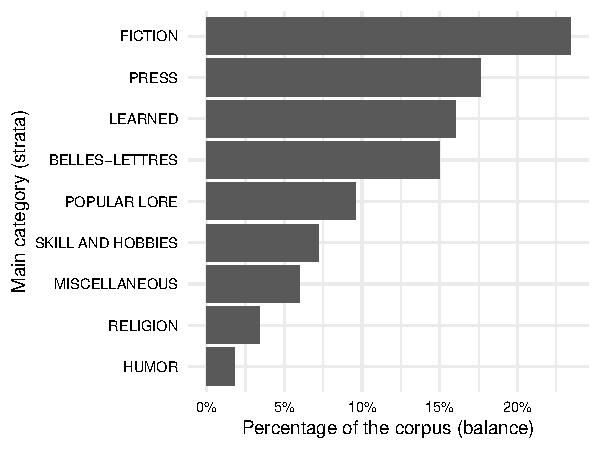
\includegraphics{part_2/2_data_files/figure-pdf/fig-data-brown-distribution-1.pdf}

}

\caption{\label{fig-data-brown-distribution}Overview of the sampling
characteristics of the Brown Corpus}

\end{figure}%

\end{minipage}%

\end{figure}%

\end{tcolorbox}

In text analysis, corpora are the raw materials of research. The aim of
the quantitative text researcher is to select the corpus, or corpora,
which best align with the purpose of the research. For example, a
reference corpus such as the American National Corpus
(\citeproc{ref-Ide2001}{Ide \& Macleod, 2001}) may be better suited to
address a question dealing with the way American English works, but this
general resource may lack detail in certain areas, such as medical
language, that may be vital for a research project aimed at
understanding changes in medical terminology. Furthermore, a researcher
studying spoken language might collect a corpus of transcribed
conversations from a particular community or region, such as the Santa
Barbara Corpus of Spoken American English (\citeproc{ref-DuBois2005}{Du
Bois et al., 2005}). While this would not include every possible spoken
utterance produced by members of that group, it could be considered a
representative sample of the population of speech in that context.

\subsection{Other considerations}\label{other-considerations}

In preparing and conducting research using corpora, the most primary
concerns is aligning research goals with the corpus resource. However,
there are other, more practical, considerations to keep in mind.

\subsubsection{Access}\label{access}

Ensuring access both in terms of physical access to the data and legal
access to the data should not be overlooked in the design and execution
of a project. Simply put, without access to the data, research cannot
proceed. It is better to consider access early in the research process
to avoid delays and complications later on.

The medium to acquire corpus data most used in contemporary quantitative
research is the internet. Although a general search query can lead you
to corpus data, there are a few primary sources of corpora you should be
aware of, summarized in Table~\ref{tbl-corpus-sources}.

\begin{longtable}[]{@{}
  >{\raggedright\arraybackslash}p{(\columnwidth - 4\tabcolsep) * \real{0.2500}}
  >{\raggedright\arraybackslash}p{(\columnwidth - 4\tabcolsep) * \real{0.4500}}
  >{\raggedright\arraybackslash}p{(\columnwidth - 4\tabcolsep) * \real{0.3000}}@{}}
\caption{Sources of corpus
data}\label{tbl-corpus-sources}\tabularnewline
\toprule\noalign{}
\begin{minipage}[b]{\linewidth}\raggedright
Source
\end{minipage} & \begin{minipage}[b]{\linewidth}\raggedright
Description
\end{minipage} & \begin{minipage}[b]{\linewidth}\raggedright
Examples
\end{minipage} \\
\midrule\noalign{}
\endfirsthead
\toprule\noalign{}
\begin{minipage}[b]{\linewidth}\raggedright
Source
\end{minipage} & \begin{minipage}[b]{\linewidth}\raggedright
Description
\end{minipage} & \begin{minipage}[b]{\linewidth}\raggedright
Examples
\end{minipage} \\
\midrule\noalign{}
\endhead
\bottomrule\noalign{}
\endlastfoot
Language repositories & Repositories that specialize in language data &
{[}Language Data Consortium{]}(https://www.ldc.upenn \\
.edu/), \href{http://talkbank.org/}{TalkBank} & & \\
Data sharing platforms & Platforms that enable researchers to securely
store, manage, and share data & {[}GitHub{]}(https:// \\
github.com), \href{https://zenodo.org}{Zenodo},
\href{https://osf.io/}{Open Science Framework} & & \\
Developed corpora & Corpora prepared by researchers for research
purposes & \href{https://ropensci.org/packages/data-access/}{APIs}, web
scraping \\
\end{longtable}

It is always advisable to start looking for data in a \textbf{language
repository}. The advantage of beginning your data search in repositories
is that a repository, especially those geared towards the linguistic
community, will make identifying language corpora faster than through a
general web search. Furthermore, repositories often require certain
standards for corpus format and documentation for publication.

\begin{tcolorbox}[enhanced jigsaw, left=2mm, toprule=.15mm, colback=white, colframe=quarto-callout-color-frame, arc=.35mm, rightrule=.15mm, bottomrule=.15mm, leftrule=.75mm, breakable, opacityback=0]

\textbf{\faIcon{lightbulb} Consider this}

Explore some of the resources listed on the Resources Kit ``Identifying
data and data sources'' guide and consider their sampling frames. Can
you think of a research question or questions that this resource may be
well-suited to support research into? What types of questions would be
less-than-adequate for a given resource?

\end{tcolorbox}

As part of a general movement towards reproducibility, more corpora are
available on \index{data!sharing platforms}\textbf{data sharing
platforms}. These platforms enable researchers to securely store,
manage, and share data with others. Support is provided for various
types of data, including documents and code, and as such they are a good
place to look as they often include reproducible research projects as
well.

Finally, if satisfactory data cannot be found in a repository or data
sharing platform, researchers may need to develop their own corpus.
There are two primary ways to attain language data from the web. The
first is through an \textbf{Application Programming Interface} (API).
APIs are, as the title suggests, programming interfaces which allow
access, under certain conditions, to information that a website or
database accessible via the web contains.

\begin{tcolorbox}[enhanced jigsaw, left=2mm, toprule=.15mm, colback=white, colframe=quarto-callout-color-frame, arc=.35mm, rightrule=.15mm, bottomrule=.15mm, leftrule=.75mm, breakable, opacityback=0]

\textbf{\faIcon{medal} Dive deeper}

The process of corpus development is a topic in and of itself. For a
more in-depth discussion of the process, see Ädel
(\citeproc{ref-Adel2020}{2020}).

\end{tcolorbox}

The second, more involved, way to acquire data from the web is is
through the process of web scraping. \textbf{Web scraping} is the
process of harvesting data from the public-facing web. Language texts
may be found on sites as uploaded files, such as pdf or doc (Word)
documents, or found displayed as the primary text of a site. Given the
wide variety of documents uploaded and language behavior recorded daily
on news sites, blogs and the like, compiling a corpus has never been
easier. Having said that, how the data is structured and how much data
needs to be retrieved can pose practical obstacles to collecting data
from the web, particularly if the approach is to acquire the data by
manually instead of automating the task.

Beyond physical access to the data, legal access is also a
consideration. Just because data is available on the web does not mean
it is free to use. Repositories, APIs, and individual data resources
often have licensing agreements and terms of use, ranging from public
domain to proprietary licenses. Respecting intellectual property rights
is crucial when working with corpus data. Violating these rights can
lead to legal and ethical issues, including lawsuits, fines, and damage
to one's professional reputation. To avoid these problems, researchers
must ensure they have the necessary permissions to use copyrighted works
in their research. Consult {``U.s. Copyright office''}
(\citeproc{ref-UScopyright2024}{n.d.}) or an academic librarian for
guidance on copyright law and fair use.

\subsubsection{Formats}\label{formats}

Whether you are using a published corpus or developing your own, it is
important to understand how the data you want to work with is formatted
so you can ensure that you are prepared to conduct the subsequent
processing steps. When referring to the format of a corpus, this
includes the folder and file structure, the file types, and how file
content is encoded electronically. Yet, the most important
characteristic, especially for language-based data, is the internal
structure of the files themselves. With this in mind less discuss the
difference between unstructured, semi-structured, and structured data.

A corpus may include various types of linguistic (\emph{e.g.} part of
speech, syntactic structure, named entities, \emph{etc.}) or
non-linguistic (\emph{e.g.} source, dates, speaker information,
\emph{etc.}) attributes. These attributes are known as
\textbf{metadata}, or data about data. As a general rule, files which
include more metadata tend to be more internally structured. Internal
file structure refers to the degree to which the content has been
formatted such that these pieces of information are easy to query and
analyze by a computer. Let's review characteristics of the three main
types of file structure types and associate common file extensions that
files in each have.

\textbf{Unstructured data} is data which does not have a
machine-readable internal structure. This is the case for plain text
files (\emph{.txt}), which are simply a sequence of characters. For
example, in Snippet~\ref{lst-masc-text} we see plain text file from the
the Manually Annotated Sub-Corpus of American English (MASC)
(\citeproc{ref-Ide2008}{Ide, Baker, Fellbaum, Fillmore, \& Passonneau,
2008}):

\begin{codelisting}

\caption{\label{lst-masc-text}MASC \emph{.txt} file}

\centering{

\begin{Shaded}
\begin{Highlighting}[]
\NormalTok{Sound is a vibration. Sound travels as a mechanical wave through a medium, and in space, there is no medium. So when my shuttle malfunctioned and the airlocks didn\textquotesingle{}t keep the air in, I heard nothing.}
\end{Highlighting}
\end{Shaded}

}

\end{codelisting}%

Other examples of files which often contain unstructured data include
\emph{.pdf} and \emph{.docx} files. While these file types may contain
data which appears structured to the human eye, the structure is not
designed to be machine-readable. As such the data would typically be
read into R as a vector of \textbf{character strings}. It is possible to
perform only the most rudimentary queries on this type of data, such as
string matches. For anything more informative, it is necessary to
further process this data, as we will see in
Section~\ref{sec-data-organization} and
Section~\ref{sec-data-transformation}.

On the other end of the spectrum, \textbf{structured data} is data which
conforms to a tabular format in which elements in tables and
relationships between tables are defined. This makes querying and
analyzing easy and efficient. Relational databases (\emph{e.g.} MySQL,
PostgreSQL, \emph{etc}.) are designed to store and query structured
data. The data frame object in R is also a structured data format. In
each case, the data is stored in a tabular format in which each row
represents a single observation and each column represents a single
attribute whose values are of the same type.

In Snippet~\ref{lst-masc-df} we see an example of an R data frame object
which overlaps with the language in the plain text file in
Snippet~\ref{lst-masc-text}:

\begin{codelisting}

\caption{\label{lst-masc-df}MASC R data frame}

\centering{

\begin{Shaded}
\begin{Highlighting}[]
\NormalTok{   doc\_id  date modality token\_id word       lemma      pos}
\NormalTok{    \textless{}}\KeywordTok{int}\NormalTok{\textgreater{} \textless{}}\KeywordTok{dbl}\NormalTok{\textgreater{} \textless{}}\KeywordTok{fct}\NormalTok{\textgreater{}       \textless{}}\KeywordTok{int}\NormalTok{\textgreater{} \textless{}}\KeywordTok{chr}\NormalTok{\textgreater{}      \textless{}}\KeywordTok{chr}\NormalTok{\textgreater{}      \textless{}}\KeywordTok{chr}\NormalTok{\textgreater{}}
\NormalTok{ 1      1  2008 Writing         1 Sound      sound      NNP}
\NormalTok{ 2      1  2008 Writing         2 is         be         VBZ}
\NormalTok{ 3      1  2008 Writing         3 a          a          DT}
\NormalTok{ 4      1  2008 Writing         4 vibration  vibration  NN}
\NormalTok{ 5      1  2008 Writing         5 .          .          .}
\NormalTok{ 6      1  2008 Writing         6 Sound      sound      NNP}
\NormalTok{ 7      1  2008 Writing         7 travels    travel     VBZ}
\NormalTok{ 8      1  2008 Writing         8 as         as         IN}
\NormalTok{ 9      1  2008 Writing         9 a          a          DT}
\NormalTok{10      1  2008 Writing        10 mechanical mechanical JJ}
\end{Highlighting}
\end{Shaded}

}

\end{codelisting}%

Here we see that the data is stored in a tabular format with each row
representing a single observation (\texttt{word}) and each column
representing a single attribute. This tabular structure supports the
increased number of metadata attributes. Internally, R applies a schema
to ensure the values in each column are of the same type (\emph{e.g.}
\texttt{\textless{}chr\textgreater{}},
\texttt{\textless{}dbl\textgreater{}},
\texttt{\textless{}fct\textgreater{}}, \emph{etc.}). This structured
format is designed to be easy to query and analyze and as such is the
primary format for data analysis in R.

\textbf{Semi-structured data} falls between unstructured and structured
data. This covers a wide range of file structuring approaches. For
example, a otherwise plain text file with part-of-speech tags appended
to each word is minimally structured, Snippet~\ref{lst-masc-pos}.

\begin{codelisting}

\caption{\label{lst-masc-pos}MASC \emph{.txt} file with part-of-speech
tags}

\centering{

\begin{Shaded}
\begin{Highlighting}[]
\NormalTok{Sound/NNP is/VBZ a/DT vibration/NN ./. Sound/NNP travels/VBZ as/IN a/DT mechanical/JJ wave/NN through/IN a/DT medium/NN ,/, and/CC in/IN space/NN ,/, there/EX is/VBZ no/DT medium/NN ./. So/RB when/WRB my/PRP$ shuttle/NN malfunctioned/JJ and/CC the/DT airlocks/NNS did/VBD n\textquotesingle{}t/RB keep/VB the/DT air/NN in/IN ,/, I/PRP heard/VBD nothing/NN ./.}
\end{Highlighting}
\end{Shaded}

}

\end{codelisting}%

Towards the more structured end of semi-structured data, many file
formats including \emph{.xml} and \emph{.json} contain hierarchical
data. For example, in Snippet~\ref{lst-masc-xml} shows a snippet from a
\emph{.xml} file from the MASC corpus.\\

\begin{codelisting}

\caption{\label{lst-masc-xml}MASC \emph{.xml} file}

\centering{

\begin{Shaded}
\begin{Highlighting}[]
\NormalTok{\textless{}}\KeywordTok{a}\OtherTok{ xml:id=}\StringTok{"penn{-}N264215"}\OtherTok{ label=}\StringTok{"tok"}\OtherTok{ ref=}\StringTok{"penn{-}n7345"}\OtherTok{ as=}\StringTok{"anc"}\NormalTok{\textgreater{}}
\NormalTok{  \textless{}}\KeywordTok{fs}\NormalTok{\textgreater{}}
\NormalTok{    \textless{}}\KeywordTok{f}\OtherTok{ name=}\StringTok{"base"}\OtherTok{ value=}\StringTok{"sound"}\NormalTok{/\textgreater{}}
\NormalTok{    \textless{}}\KeywordTok{f}\OtherTok{ name=}\StringTok{"msd"}\OtherTok{ value=}\StringTok{"NNP"}\NormalTok{/\textgreater{}}
\NormalTok{    \textless{}}\KeywordTok{f}\OtherTok{ name=}\StringTok{"string"}\OtherTok{ value=}\StringTok{"Sound"}\NormalTok{/\textgreater{}}
\NormalTok{  \textless{}/}\KeywordTok{fs}\NormalTok{\textgreater{}}
\NormalTok{\textless{}/}\KeywordTok{a}\NormalTok{\textgreater{}}
\NormalTok{\textless{}}\KeywordTok{node}\OtherTok{ xml:id=}\StringTok{"penn{-}n7346"}\NormalTok{\textgreater{}}
\NormalTok{  \textless{}}\KeywordTok{link}\OtherTok{ targets=}\StringTok{"seg{-}r13152"}\NormalTok{/\textgreater{}}
\NormalTok{\textless{}/}\KeywordTok{node}\NormalTok{\textgreater{}}
\NormalTok{\textless{}}\KeywordTok{a}\OtherTok{ xml:id=}\StringTok{"penn{-}N264243"}\OtherTok{ label=}\StringTok{"tok"}\OtherTok{ ref=}\StringTok{"penn{-}n7346"}\OtherTok{ as=}\StringTok{"anc"}\NormalTok{\textgreater{}}
\NormalTok{  \textless{}}\KeywordTok{fs}\NormalTok{\textgreater{}}
\NormalTok{    \textless{}}\KeywordTok{f}\OtherTok{ name=}\StringTok{"string"}\OtherTok{ value=}\StringTok{"is"}\NormalTok{/\textgreater{}}
\NormalTok{    \textless{}}\KeywordTok{f}\OtherTok{ name=}\StringTok{"msd"}\OtherTok{ value=}\StringTok{"VBZ"}\NormalTok{/\textgreater{}}
\NormalTok{    \textless{}}\KeywordTok{f}\OtherTok{ name=}\StringTok{"base"}\OtherTok{ value=}\StringTok{"be"}\NormalTok{/\textgreater{}}
\NormalTok{  \textless{}/}\KeywordTok{fs}\NormalTok{\textgreater{}}
\NormalTok{\textless{}/}\KeywordTok{a}\NormalTok{\textgreater{}}
\NormalTok{\textless{}}\KeywordTok{node}\OtherTok{ xml:id=}\StringTok{"penn{-}n7347"}\NormalTok{\textgreater{}}
\NormalTok{  \textless{}}\KeywordTok{link}\OtherTok{ targets=}\StringTok{"seg{-}r13154"}\NormalTok{/\textgreater{}}
\NormalTok{\textless{}/}\KeywordTok{node}\NormalTok{\textgreater{}}
\end{Highlighting}
\end{Shaded}

}

\end{codelisting}%

The format of semi-structured data is often influenced by
characteristics of the data or reflect an author's individual
preferences. It is sometimes the case that data will be semi-structured
in a less-standard format. For example, the Switchboard Dialog Act
corpus (SWDA) (\citeproc{ref-SWDA2008}{University of Colorado Boulder,
2008}), in Snippet~\ref{lst-swda-utt}, includes a \emph{.utt} file
extension for files which contain utterances annotated with dialog act
tags.

\begin{codelisting}

\caption{\label{lst-swda-utt}SWDA \emph{.utt} file}

\centering{

\begin{Shaded}
\begin{Highlighting}[]
\NormalTok{o      A.1 utt1: Okay. /}
\NormalTok{qw     A.1 utt2: \{D So, \}}
\NormalTok{qy\^{}d   B.2 utt1: [ [ I guess, +}
\NormalTok{+      A.3 utt1: What kind of experience [ do you, + do you ] have, then with child care? /}
\NormalTok{+      B.4 utt1: I think, ] + \{F uh, \} I wonder ] if that worked. /}
\NormalTok{qy     A.5 utt1: Does it say something? /}
\end{Highlighting}
\end{Shaded}

}

\end{codelisting}%

Whether standard or not, semi-structured data is often designed to be
machine-readable. As with unstructured data, the ultimate goal is to
convert the data into a structured format and augment the data where
necessary to prepare it for a particular research analysis.

\section{Information}\label{information}

Identifying an adequate corpus resource, in terms of content, access,
and formatting, for the target research question is the first step in
moving a quantitative text research project forward. The next step is to
select the components or characteristics of this resource that are
relevant for the research and then move to organize the attributes of
this data into a more informative format. This is the process of
converting corpus data into a \index{dataset}\textbf{dataset} --a
tabular representation of particular attributes of the data as the basis
for generating information. Once the data represented as dataset, it is
often manipulated and transformed adjusting and augmenting the data such
that it better aligns with the research question and the target
analytical approach.

\subsection{Organization}\label{sec-data-organization}

Data alone is not informative. Only through explicit organization of the
data in a way that makes relationships and meaning explicit does data
become information. In this form, our data is called a dataset. This is
a particularly salient hurdle in text analysis research. Many textual
sources are unstructured or semi-structured. This means relationships
that will be used in the analysis have yet to be purposefully drawn and
organized as a dataset.

\subsubsection{Tidy Data}\label{sec-data-tidy-data}

The selection of the attributes from a corpus and the juxtaposition of
these attributes in a relational format, or dataset, that converts data
into information is known as \textbf{data curation}. The process of data
curation minimally involves deriving a base dataset, or \emph{curated
dataset}, which establishes the main informational associations
according to philosophical approach outlined by Wickham
(\citeproc{ref-Wickham2014a}{2014}).

In this work, a \textbf{tidy dataset} refers both to the structural
(physical) and informational (semantic) organization of the dataset.
Physically, a tidy dataset is a tabular data structure, illustrated in
Figure~\ref{fig-data-tidy-format-image}, where each \emph{row} is an
observation and each \emph{column} is a variable that contains measures
of a feature or attribute of each observation. Each cell where a given
row-column intersect contains a \emph{value} which is a particular
attribute of a particular observation for the particular
observation-feature pair also known as a \emph{data point}.

\begin{figure}[!htb]

\centering{

{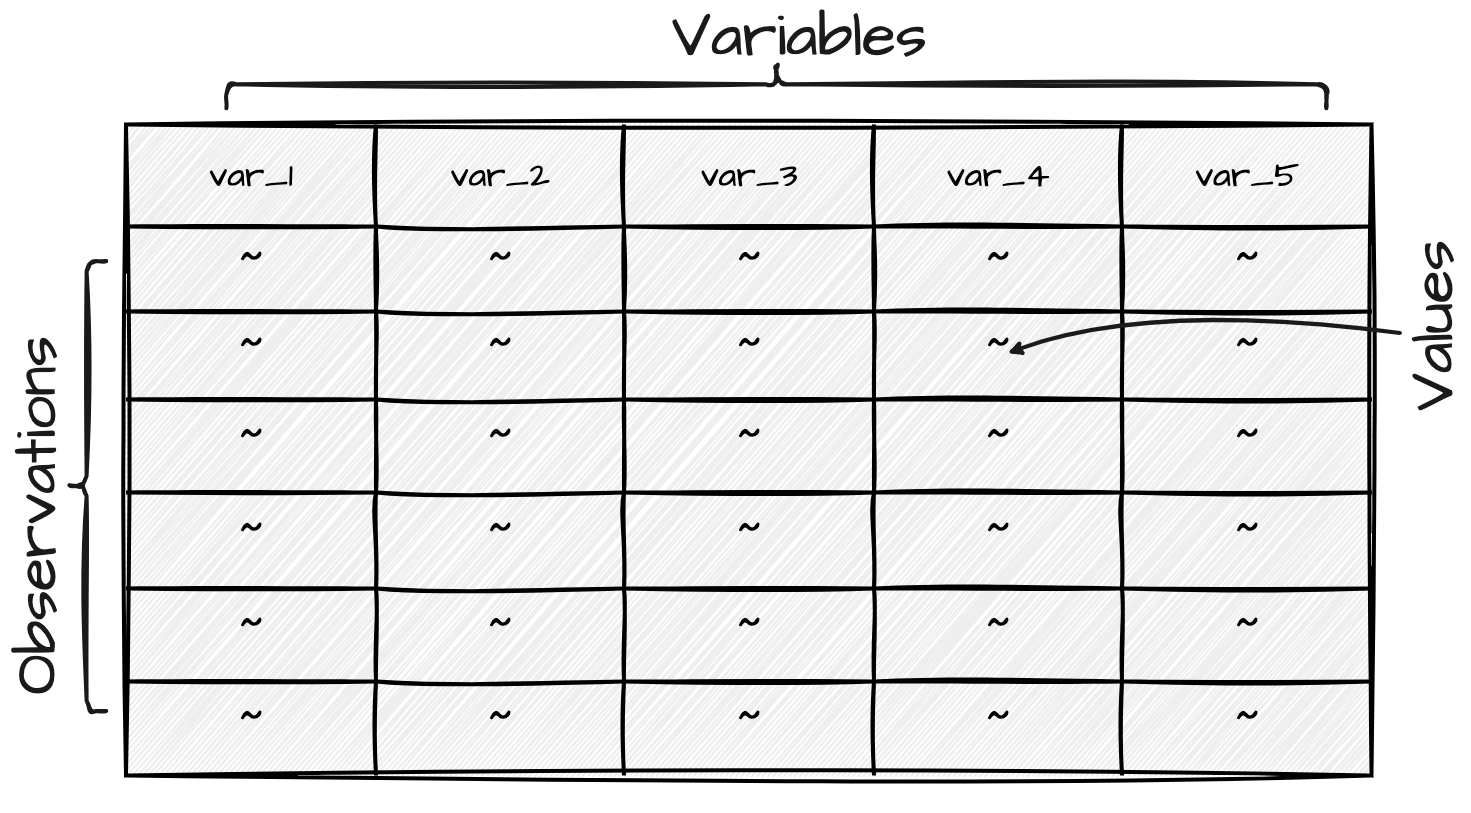
\includegraphics{part_2/figures/data-tidy.drawio.png}}

}

\caption{\label{fig-data-tidy-format-image}Visual summary of the tidy
dataset format}

\end{figure}%

In terms of semantics, columns and rows both contribute to the
informational value of the dataset. Let's start with columns. In a tidy
dataset, each column is a variable, an attribute that can take on a
number of values. Although variables vary in terms of values, they do
not in type. A variable is of one and only one informational type.
Statistically speaking, informational types are defined as
\textbf{levels of measurement}, a classification system used to
semantically distiguish between types of variables. There are four
levels (or types) in this system: nominal, ordinal, interval, and ratio.

In practice, however, text analysis researchers often group these levels
into three main informational types: categorical, ordinal, and numeric
(\citeproc{ref-Gries2021a}{S. T. Gries, 2021}). What do these
informational types represent? \textbf{Categorical data} is for labeled
data or classes that answer the question ``what?'' \textbf{Ordinal data}
is categorical data with rank order that answers the question ``what
order?'' \textbf{Numeric data} is ordinal data with equal intervals
between values that answers the question ``how much or how many?''

Let's look at an example of a tidy dataset. Using the criteria just
described, let's see if we can identify the informational values
(categorical, ordinal, or numeric) of the variables that appear in a
snippet from the MASC corpus in dataset form in
Table~\ref{tbl-data-info-values-masc}.

\begin{longtable}[]{@{}
  >{\raggedright\arraybackslash}p{(\columnwidth - 12\tabcolsep) * \real{0.1400}}
  >{\raggedright\arraybackslash}p{(\columnwidth - 12\tabcolsep) * \real{0.1400}}
  >{\raggedright\arraybackslash}p{(\columnwidth - 12\tabcolsep) * \real{0.1400}}
  >{\raggedright\arraybackslash}p{(\columnwidth - 12\tabcolsep) * \real{0.1400}}
  >{\raggedright\arraybackslash}p{(\columnwidth - 12\tabcolsep) * \real{0.1600}}
  >{\raggedright\arraybackslash}p{(\columnwidth - 12\tabcolsep) * \real{0.1400}}
  >{\raggedright\arraybackslash}p{(\columnwidth - 12\tabcolsep) * \real{0.1400}}@{}}

\caption{\label{tbl-data-info-values-masc}MASC dataset variables}

\tabularnewline

\toprule\noalign{}
\begin{minipage}[b]{\linewidth}\raggedright
doc\_id
\end{minipage} & \begin{minipage}[b]{\linewidth}\raggedright
modality
\end{minipage} & \begin{minipage}[b]{\linewidth}\raggedright
date
\end{minipage} & \begin{minipage}[b]{\linewidth}\raggedright
token\_id
\end{minipage} & \begin{minipage}[b]{\linewidth}\raggedright
word
\end{minipage} & \begin{minipage}[b]{\linewidth}\raggedright
pos
\end{minipage} & \begin{minipage}[b]{\linewidth}\raggedright
num\_let
\end{minipage} \\
\midrule\noalign{}
\endhead
\bottomrule\noalign{}
\endlastfoot
1 & Writing & 2008 & 1 & Sound & NNP & 5 \\
1 & Writing & 2008 & 2 & is & VBZ & 2 \\
1 & Writing & 2008 & 3 & a & DT & 1 \\
1 & Writing & 2008 & 4 & vibration & NN & 9 \\
1 & Writing & 2008 & 5 & . & . & 1 \\
1 & Writing & 2008 & 6 & Sound & NNP & 5 \\
1 & Writing & 2008 & 7 & travels & VBZ & 7 \\
1 & Writing & 2008 & 8 & as & IN & 2 \\
1 & Writing & 2008 & 9 & a & DT & 1 \\
1 & Writing & 2008 & 10 & mechanical & JJ & 10 \\

\end{longtable}

We have seven variables listed as headers for each of the columns. We
could go one-by-one left-to-right but let's take another tack. Instead,
let's identify all those variables that cannot be numeric --these are
all the non-numeral variables: \texttt{modality}, \texttt{word}, and
\texttt{pos}. The question to ask of these variables is whether they
represent an order or rank. Since modalities, words, and parts-of-speech
are not ordered values, they are all categorical.

Now in relation to \texttt{doc\_id}, \texttt{date}, \texttt{token\_id},
and \texttt{num\_let}. All four are numerals, so they could be numeric.
But they could also be numeral representations of categorical or ordinal
data. Before we can move forward, we need to make sure we understand
what each variable means and how it is measured, or
\textbf{operationalized}. The variable name and the values can be
helpful in this respect. \texttt{doc\_id} and \texttt{token\_id} are
unique identifiers for each document and word. \texttt{date} is what it
sounds like, a date, and is operationalized as a year in the Gregorian
calendar. And \texttt{num\_let} seems quite descriptive as well, number
of letters, appearing as a letter count.

With this in mind, let's return to the question of whether these
variables are numeric, ordinal, or categorical. Starting with the
trickiest one, \texttt{date}, we can ask the question to identify
numeric data: ``how much or how many?''. In the case of \texttt{date},
the answer is neither. A date is a point in time, not a quantity. So
\texttt{date} is not numeric. But it does provide information about
order. Hence, \texttt{date} is ordinal. Next, \texttt{num\_let} is
numeric because it answers the question ``how many?''. Now,
\texttt{doc\_id} and \texttt{token\_id} are both identifiers, so they
are not numeric, but the question is whether they encode order as well.
In this case, it depends. If the identifiers are assigned in a way that
reflects the order of the documents or tokens, then they are ordinal. It
is more likely the case that the \texttt{doc\_id} is not ordinal, but
the \texttt{token\_id} is. This is because the \texttt{token\_id} is
likely assigned in the order the words appear in the document.

Let's turn to the second semantic value of a tidy dataset. In a tidy
dataset, each row is an observation. But an observation of what? This
depends on what the unit of observation is. That sounds circular, but
its not. The \textbf{unit of observation} is simply the primary entity
that is being observed or measured
(\citeproc{ref-Sedgwick2015}{Sedgwick, 2015}). Even without context, it
can often be identified in a dataset by looking at the level of
specificity of the variable values and asking what each variable
describes. When one variable appears to be the most individualized and
other variables appear to describe that variable, then the most
individualized variable is likely the unit of observation of the
dataset, \emph{i.e.} the meaning of each observation.

Applying these strategies to the Table in
\ref{tbl-data-info-values-masc}, we can see that each observation at its
core is a word. We see that the values of each observation are the
attributes of each word. \texttt{word} is the most individualized
variable and the \texttt{pos} (part-of-speech), \texttt{num\_let}, and
\texttt{token\_id} all describe the word.

The other variables \texttt{doc\_id}, \texttt{modality}, and
\texttt{date} are not direct attributes of the word. Instead, they are
attributes of the document in which the word appears. Together, however,
they all provide information about the word.

\begin{tcolorbox}[enhanced jigsaw, left=2mm, toprule=.15mm, colback=white, colframe=quarto-callout-color-frame, arc=.35mm, rightrule=.15mm, bottomrule=.15mm, leftrule=.75mm, breakable, opacityback=0]

\textbf{\faIcon{lightbulb} Consider this}

Data can be organized in many ways. It is important to make clear that
data in tabular format in itself does not constitute a dataset, in the
tidy sense we will be using. Can you think of examples of tabular
information that would not be in a tidy format? What would be the
implications of this for data analysis?

\end{tcolorbox}

As we round out this section on data organization, it is important to
stress that the purpose of curation is to represent the corpus data in
an informative, tidy format. A curated dataset serves as a reference
point making relationships explicit, enabling more efficient querying,
and paving the way for further processing before analysis.

\subsection{Transformation}\label{sec-data-transformation}

At this point have introduced the first step towards creating a dataset
ready for analysis, data curation. However, a curated dataset is rarely
the final organizational step before proceeding to statistical analysis.
Many times, if not always, the curated dataset requires
\textbf{transformation} to derive or generate new data for the dataset.
This process may incur row-wise (observation) or column-wise (variable)
level changes, as illustrated in Figure~\ref{fig-data-transformations}.

\begin{figure}[!htb]

\centering{

{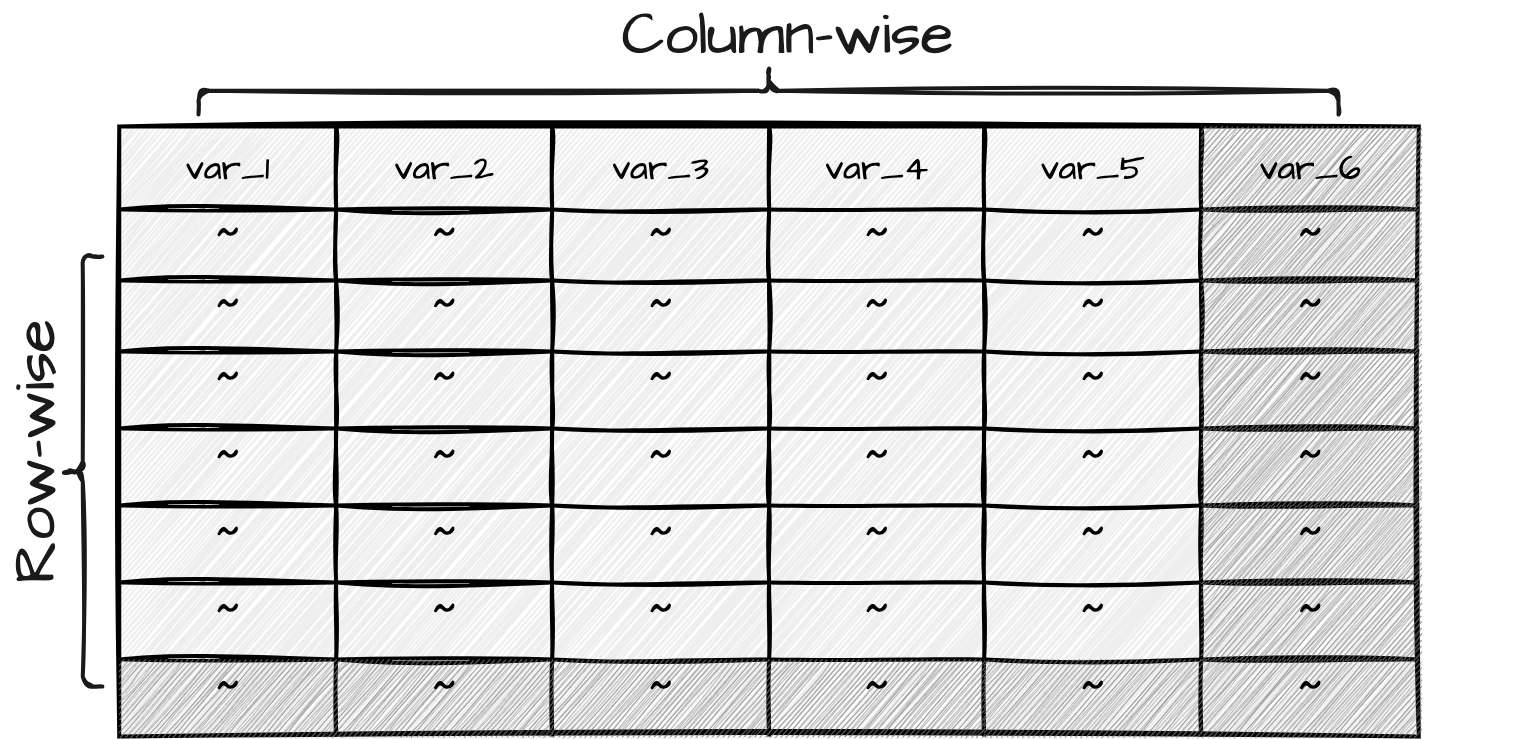
\includegraphics{part_2/figures/data-transformations.drawio.png}}

}

\caption{\label{fig-data-transformations}Visualization of row-wise and
column-wise transformation operations on a dataset}

\end{figure}%

The results build on and manipulate the curated dataset to produce a
\emph{transformed dataset}. While there is typically one curated dataset
that serves as the base organizational dataset, there may be multiple
transformed datasets, each aligning with the informational needs of
specific analyses in the research project.

In what follows, we will group common transformation processes into two
purpose-based groupings: preparation and enrichment. The process may
include one or more of the subsequent transformations but is rarely
linear and is most often iterative. The bottom line is, however, to make
the dataset more informative and more amenable to the particular aims of
a given analysis.

\subsubsection{Preparation}\label{preparation}

The purpose of preparation transformations is to clean, standardize, and
derive the key attributes of the dataset on which further processing
will depend. Common preparation transformations include text
normalization and text tokenization.

Let's take a toy dataset, in Table~\ref{tbl-data-text-dataset}, as a
starting point for exploring various transformations. In this dataset,
we have three variables, \texttt{text\_id}, \texttt{sent\_id}, and
\texttt{sentence}. It has five observations.

\begin{longtable}[]{@{}
  >{\raggedright\arraybackslash}p{(\columnwidth - 4\tabcolsep) * \real{0.1000}}
  >{\raggedright\arraybackslash}p{(\columnwidth - 4\tabcolsep) * \real{0.1000}}
  >{\raggedright\arraybackslash}p{(\columnwidth - 4\tabcolsep) * \real{0.8000}}@{}}

\caption{\label{tbl-data-text-dataset}A toy dataset with three
variables, \texttt{text\_id}, \texttt{sent\_id}, and \texttt{sentence}}

\tabularnewline

\toprule\noalign{}
\begin{minipage}[b]{\linewidth}\raggedright
text\_id
\end{minipage} & \begin{minipage}[b]{\linewidth}\raggedright
sent\_id
\end{minipage} & \begin{minipage}[b]{\linewidth}\raggedright
sentence
\end{minipage} \\
\midrule\noalign{}
\endhead
\bottomrule\noalign{}
\endlastfoot
1 & 1 & It's a beautiful day in the US, and our group decided to visit
the famous Grand Canyon. \\
1 & 2 & As we reached the destination, Jane said, ``I can't believe
we're finally here!'' \\
1 & 3 & The breathtaking view left us speechless; indeed, it was a sight
to behold. \\
1 & 4 & During our trip, we encountered tourists from different
countries, sharing stories and laughter. \\
1 & 5 & For all of us, this experience will be cherished forever. \\

\end{longtable}

\textbf{Text normalization} is the process of standardizing text to
convert the text into a uniform format and reduce unwanted variation and
noise. It is often a preliminary step in data transformation processes
which include variables with text.

The normalization we apply will depend on the specific needs of the
project, but can include operations such as changing the case of the
text, removing punctuation, standardizing forms, \emph{etc.} The goal is
to reduce the noise in the text and make it more amenable to analysis.

Normalization tends to preserve the number of rows and columns in the
dataset but \emph{does} change the values of the variables. These tasks
should be applied with an understanding of how the changes will impact
the analysis. For example, looking at tbl-data-text-dataset, lowercasing
can be useful for reducing differences between words that are otherwise
identical, yet differ in case due to word position in a sentence
(``The'' versus ``the''). However, lowercasing can also be problematic
if the case of the word carries semantic value, such as in the case of
``US'' (United States) and ``us'' (first-person plural pronoun).

\textbf{Text tokenization} involves adapting the text such that it
reflects the target linguistic unit that will be used in the analysis.
This is a row-wise operation expanding the number of rows, if the
linguistic unit is smaller than the original variable, or reducing the
number of rows, if the linguistic unit is larger than the original
variable.

Text variables can be tokenized at any linguistic level, to the extent
we can operationalize the linguistic unit. The operationalized
linguistic unit is known as a \textbf{term}. For example, terms can be
characters, words, sentences, \emph{etc}. When we refer to the
individual units of term, we use the expression \textbf{tokens}. Another
key term to introduce is \textbf{types}, which refers to the unique
tokens in a term variable. For example, in the sentence 1 in
Table~\ref{tbl-data-text-dataset}, there are 16 types and 17 tokens --as
`the' is repeated. Note that there will always be at least as many
tokens as types, but there can be many more tokens than types for any
given term variable.

Sequential groupings of characters and words are also common terms used
in text analysis. These are known as \textbf{\(n\)-grams}, where \(n\)
is the number of words or characters in the term. For example, a word
bigram is a sequence of two words, and a character trigram is a sequence
of three characters.

\begin{table}

\caption{\label{tbl-data-tokenization}Word and character tokenization
examples}

\begin{minipage}{0.50\linewidth}

\subcaption{\label{tbl-data-tokenization-1}Character trigram tokenization}

\centering{

\begin{tabular}{lll}
\toprule
text\_id & sent\_id & trigram\\
\midrule
1 & 1 & its\\
1 & 1 & tsa\\
1 & 1 & sab\\
1 & 1 & abe\\
1 & 1 & bea\\
1 & 1 & eau\\
1 & 1 & aut\\
1 & 1 & uti\\
1 & 1 & tif\\
1 & 1 & ifu\\
\bottomrule
\end{tabular}

}

\end{minipage}%
%
\begin{minipage}{0.50\linewidth}

\subcaption{\label{tbl-data-tokenization-2}Word bigram tokenization}

\centering{

\begin{tabular}{lll}
\toprule
text\_id & sent\_id & bigram\\
\midrule
1 & 1 & it's a\\
1 & 1 & a beautiful\\
1 & 1 & beautiful day\\
1 & 1 & day in\\
1 & 1 & in the\\
1 & 1 & the us\\
1 & 1 & us and\\
1 & 1 & and our\\
1 & 1 & our group\\
1 & 1 & group decided\\
\bottomrule
\end{tabular}

}

\end{minipage}%

\end{table}%

\begin{tcolorbox}[enhanced jigsaw, left=2mm, toprule=.15mm, colback=white, colframe=quarto-callout-color-frame, arc=.35mm, rightrule=.15mm, bottomrule=.15mm, leftrule=.75mm, breakable, opacityback=0]

\textbf{\faIcon{file-alt} Case study}

Serigos (\citeproc{ref-Serigos2020}{2020}) explores the social
stratification of anglicisms in Argentine media. The author presents a
method for automatically detecting anglicisms in Spanish texts. In
combination with other methods, character \(n\)-grams are used to
determine the language of a word. The method is based on the observation
that the distribution of character \(n\)-grams is different between
languages.

\end{tcolorbox}

In Table~\ref{tbl-data-tokenization}, we see examples of tokenization at
word and character levels. At its core, tokenization is the process
which enables the quantitative analysis of text. Choosing the right
tokenization level is crucial for the success of the analysis.

\subsubsection{Enrichment}\label{enrichment}

Enrichment transformations are designed to add new attributes to the
dataset. These attributes may be derived from the existing attributes or
may be integrated from other datasets. Common enrichment transformations
include generation, recoding, and integration of observations and/ or
variables.

\textbf{Generation} is the process of creating new variables based on
implicit information within existing variables. It is a row- and
column-wise operation which in text analysis often includes linguistic
annotation such as part-of-speech tagging, morphological analysis,
syntactic parsing, \emph{etc.} These annotations can be used to generate
new variables that capture linguistic information that is not explicitly
present in the text.

Linguistic annotation can be done manually by linguist coders and/ or
done automatically using natural language processing (NLP) tools. To
illustrate the process of automatic linguistic annotation, we will start
with the dataset from Table~\ref{tbl-data-text-dataset}. Applying a
pre-trained English model (\citeproc{ref-Silveira2014}{Silveira et al.,
2014}) from the Universal Dependencies (UD) project
(\citeproc{ref-DeMarneffe2021}{de Marneffe, Manning, Nivre, \& Zeman,
2021}), we can generate linguistic annotation for each word in the
\texttt{sentence} variable.

\begin{longtable}[]{@{}
  >{\raggedright\arraybackslash}p{(\columnwidth - 8\tabcolsep) * \real{0.0200}}
  >{\raggedright\arraybackslash}p{(\columnwidth - 8\tabcolsep) * \real{0.0900}}
  >{\raggedright\arraybackslash}p{(\columnwidth - 8\tabcolsep) * \real{0.0500}}
  >{\raggedright\arraybackslash}p{(\columnwidth - 8\tabcolsep) * \real{0.7400}}
  >{\raggedright\arraybackslash}p{(\columnwidth - 8\tabcolsep) * \real{0.1000}}@{}}

\caption{\label{tbl-data-generate-annotation}Automatic linguistic
annotation example}

\tabularnewline

\toprule\noalign{}
\begin{minipage}[b]{\linewidth}\raggedright
id
\end{minipage} & \begin{minipage}[b]{\linewidth}\raggedright
token
\end{minipage} & \begin{minipage}[b]{\linewidth}\raggedright
pos
\end{minipage} & \begin{minipage}[b]{\linewidth}\raggedright
feats
\end{minipage} & \begin{minipage}[b]{\linewidth}\raggedright
relation
\end{minipage} \\
\midrule\noalign{}
\endhead
\bottomrule\noalign{}
\endlastfoot
1 & As & IN & NA & mark \\
2 & we & PRP &
Case=Nom\textbar Number=Plur\textbar Person=1\textbar PronType=Prs &
nsubj \\
3 & reached & VBD & Mood=Ind\textbar Tense=Past\textbar VerbForm=Fin &
advcl \\
4 & the & DT & Definite=Def\textbar PronType=Art & det \\
5 & destination & NN & Number=Sing & obj \\
6 & , & , & NA & punct \\
7 & Jane & NNP & Number=Sing & nsubj \\
8 & said & VBD & Mood=Ind\textbar Tense=Past\textbar VerbForm=Fin &
root \\
9 & , & , & NA & punct \\
10 & '' & `` & NA & punct \\
11 & I & PRP &
Case=Nom\textbar Number=Sing\textbar Person=1\textbar PronType=Prs &
nsubj \\
12 & ca & MD & VerbForm=Fin & aux \\
13 & n't & RB & NA & advmod \\
14 & believe & VB & VerbForm=Inf & ccomp \\
15 & we & PRP &
Case=Nom\textbar Number=Plur\textbar Person=1\textbar PronType=Prs &
nsubj \\
16 & 're & VBP & Mood=Ind\textbar Tense=Pres\textbar VerbForm=Fin &
cop \\
17 & finally & RB & NA & advmod \\
18 & here & RB & PronType=Dem & ccomp \\
19 & ! & . & NA & punct \\
20 & '' & '\,' & NA & punct \\

\end{longtable}

The annotated dataset is now tokenized by word and includes the key
variables \texttt{pos}
(\href{https://www.ling.upenn.edu/courses/Fall_2003/ling001/penn_treebank_pos.html}{Penn
treebank tagset}), \texttt{feats} (morphological features), and
\texttt{relation} (dependency relations). These variables provide
information about the grammatical category and syntactic structure of
each word in the sentence. The results of this process enables more
direct access during analysis to features that were hidden or otherwise
difficult to access.

\begin{tcolorbox}[enhanced jigsaw, left=2mm, toprule=.15mm, colback=white, colframe=quarto-callout-color-frame, arc=.35mm, rightrule=.15mm, bottomrule=.15mm, leftrule=.75mm, breakable, opacityback=0]

\textbf{\faIcon{exclamation-triangle} Warning}

Automated linguistic annotation can offer rapid access to abundant and
highly dependable linguistic data for numerous languages. However,
linguistic annotation tools are not infallible. They are tools developed
by training computational algorithms to identify patterns in previously
annotated and verified datasets, resulting in a language model. This
model is then employed to predict linguistic annotations for new
language data. The accuracy of the linguistic annotation heavily relies
on the congruence between the language sampling frame of the trained
data and that of the dataset to be automatically annotated.

\end{tcolorbox}

\textbf{Recoding} is the process of transforming the values of one or
more variables into new values which are more amenable to analysis. This
is a column-wise operation which is used to make explicit information
more accessible. Typical operatins include extraction, reclassification,
and calculation.

In terms of \textbf{extraction}, the goal is to distill relevant
information from existing variables. For example, extracting the year
from a date variable, or extracting the first name from a full name
variable. In text analysis, extraction is often used to extract
information from text variables. Say we have a dataset with a variable
containing conversation utterances. We may want to extract some
characteristic from those utterances and capture their occurrence in a
new variable.

\textbf{Reclassification} aims to simplify complex variables, making it
easier to identify patterns and trends relevant for the research
question. For example, the surface forms of words can be reduced to
their stemmed or lemmatized forms. \textbf{Stemming} is the process of
reducing inflected words to their word stem, base, or root form.
\textbf{Lemmatization} is the process of reducing inflected words to
their dictionary form, or lemma.

In Table~\ref{tbl-data-recode-categorical-lemma}, we see an example of
recoding surface forms of words to their stemmed and lemmatized forms.

\begin{longtable}[]{@{}
  >{\raggedright\arraybackslash}p{(\columnwidth - 8\tabcolsep) * \real{0.2000}}
  >{\raggedright\arraybackslash}p{(\columnwidth - 8\tabcolsep) * \real{0.2000}}
  >{\raggedright\arraybackslash}p{(\columnwidth - 8\tabcolsep) * \real{0.2000}}
  >{\raggedright\arraybackslash}p{(\columnwidth - 8\tabcolsep) * \real{0.2000}}
  >{\raggedright\arraybackslash}p{(\columnwidth - 8\tabcolsep) * \real{0.2000}}@{}}

\caption{\label{tbl-data-recode-categorical-lemma}Reclassification of
surface forms of words to their stemmed and lemmatized forms}

\tabularnewline

\toprule\noalign{}
\begin{minipage}[b]{\linewidth}\raggedright
text\_id
\end{minipage} & \begin{minipage}[b]{\linewidth}\raggedright
sent\_id
\end{minipage} & \begin{minipage}[b]{\linewidth}\raggedright
word
\end{minipage} & \begin{minipage}[b]{\linewidth}\raggedright
stem
\end{minipage} & \begin{minipage}[b]{\linewidth}\raggedright
lemma
\end{minipage} \\
\midrule\noalign{}
\endhead
\bottomrule\noalign{}
\endlastfoot
1 & 2 & as & a & as \\
1 & 2 & we & we & we \\
1 & 2 & reached & reach & reach \\
1 & 2 & the & the & the \\
1 & 2 & destination & destin & destination \\
1 & 2 & jane & jane & jane \\
1 & 2 & said & said & say \\
1 & 2 & i & i & i \\
1 & 2 & can & can & can \\
1 & 2 & not & not & not \\
1 & 2 & believe & believ & believe \\
1 & 2 & we & we & we \\
1 & 2 & are & are & be \\
1 & 2 & finally & final & finally \\
1 & 2 & here & here & here \\

\end{longtable}

\begin{tcolorbox}[enhanced jigsaw, left=2mm, toprule=.15mm, colback=white, colframe=quarto-callout-color-frame, arc=.35mm, rightrule=.15mm, bottomrule=.15mm, leftrule=.75mm, breakable, opacityback=0]

\textbf{\faIcon{file-alt} Case study}

Inflectional family size is the number of inflectional forms for a given
word and can be calculated from a corpus by counting the number of
surface forms for each lemma in the corpus
(\citeproc{ref-Kostic2003}{Kostić, Marković, \& Baucal, 2003}). R.
Harald Baayen, Feldman, \& Schreuder (\citeproc{ref-Baayen2006}{2006})
found that words with larger inflectional family size are associated
with faster word recognition times in lexical processing tasks.

\end{tcolorbox}

Reclassification transformations can be useful for simplifying complex
variables, making it easier to identify patterns, as we see in
Table~\ref{tbl-data-recode-categorical-lemma}. However, it is important
to consider the trade-offs of reclassification and to ensure that the
result aligns with the research question. For example, reclassifying a
numeric variable to a categorical variable or a categorical variable
into a variable with fewer levels variable can lead to loss of
information about the original levels (\citeproc{ref-Baayen2010}{R.
Harald Baayen, 2010}).

\textbf{Calculations} of measures can also be seen as a recoding
operation. In text analysis, measures are often used to describe the
properties of a document or linguistic unit. For example, the number of
words in a corpus document, the lengths of sentences, the number of
clauses in a sentence, \emph{etc.} In turn, these measures can be used
to calculate other measures, such as lexical diversity or syntactic
complexity measures. The end result makes the dataset more informative
and amenable to analysis.

\textbf{Integration} is a transformation step which can be row-wise or
column-wise. Row-wise integration is the process of combining datasets
by appending observations from one dataset to another. Column-wise
integration is the process of combining datasets by appending variables
from one dataset to another.

To integrate in row-wise manner the datasets involved in the process
must have the same variables and variable types. This process is often
referred to as \textbf{concatenating datasets}, and is visualized in
Figure~\ref{fig-concatenating}. It can be thought of as stacking
datasets on top of each other to create a larger dataset. Remember,
having the same variables and variable types is not the same has having
the same values.

Take, for example, a case when a corpus resource contains data for two
populations. In the course of curating and transforming the datasets, it
may make more sense to work with the datasets separately. However, when
it comes time to analyze the data, it may be more convenient to work
with the datasets as a single dataset. In this case, the datasets can be
concatenated to create a single dataset.

\begin{figure}[!htb]

\begin{minipage}{0.40\linewidth}

\centering{

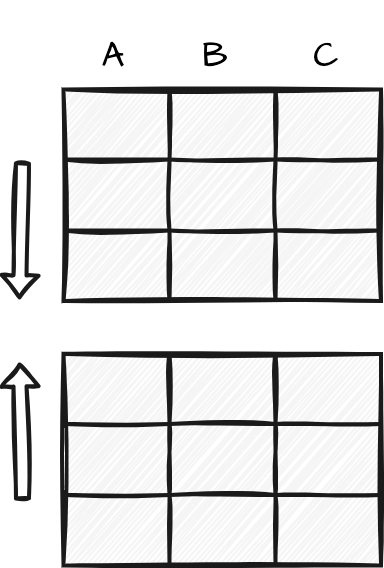
\includegraphics{part_2/figures/integration-concat-visual.drawio.png}

}

\subcaption{\label{fig-concatenating}Concatenating}

\end{minipage}%
%
\begin{minipage}{0.05\linewidth}
~\end{minipage}%
%
\begin{minipage}{0.55\linewidth}

\centering{

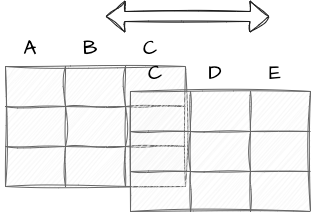
\includegraphics{part_2/figures/integration-join-visual.drawio.png}

}

\subcaption{\label{fig-joining}Joining}

\end{minipage}%

\caption{\label{fig-data-integration}Visual summary of row-wise and
column-wise integration operations on datasets}

\end{figure}%

Integrating datasets can be performed in a column-wise manner as well.
In this process, the datasets need not have the exact same variables and
variable types, rather it is required that the datasets share a common
variable of the same informational type that can be used to index the
datasets. This process is often referred to as \textbf{joining datasets}
and is visualized in Figure~\ref{fig-joining}.

Corpus resources often include metadata in stand-off annotation format.
That is, the metadata is not embedded in the corpus files, but rather is
stored in a separate file. The metatdata and corpus files will share a
common variable which can be used to join the metadata with the corpus
files, in turn creating a more informative dataset.

\section{Documentation}\label{sec-data-documentation}

As we have seen in this chapter, acquiring corpus data and converting
that data into information involves a number of conscious decisions and
implementation steps. As a favor to ourselves, as researchers, and to
the research community, it is crucial to document these decisions and
steps. Documentation includes a data origin file for the acquired corpus
data, data dictionaries for the curated and transformed datasets, and
well-documented code for the processing steps.

\subsection{Data origin}\label{sec-data-data-origin}

Data acquired from corpus resources should be accompanied by information
about the \textbf{data origin}. Table~\ref{tbl-data-data-origin}
provides a list of the types of information that should be included in
the data origin information.

\begin{longtable}[]{@{}
  >{\raggedright\arraybackslash}p{(\columnwidth - 2\tabcolsep) * \real{0.2500}}
  >{\raggedright\arraybackslash}p{(\columnwidth - 2\tabcolsep) * \real{0.7500}}@{}}
\caption{Data origin
information}\label{tbl-data-data-origin}\tabularnewline
\toprule\noalign{}
\begin{minipage}[b]{\linewidth}\raggedright
Information
\end{minipage} & \begin{minipage}[b]{\linewidth}\raggedright
Description
\end{minipage} \\
\midrule\noalign{}
\endfirsthead
\toprule\noalign{}
\begin{minipage}[b]{\linewidth}\raggedright
Information
\end{minipage} & \begin{minipage}[b]{\linewidth}\raggedright
Description
\end{minipage} \\
\midrule\noalign{}
\endhead
\bottomrule\noalign{}
\endlastfoot
Resource name & Name of the corpus resource. \\
Data source & URL, DOI, \emph{etc.} \\
Data sampling frame & Language, language variety, modality, genre,
\emph{etc.} \\
Data collection date(s) & The date or date range of the data
collection. \\
Data format & Plain text, XML, HTML, \emph{etc.} \\
Data schema & Relationships between data elements: files, folders,
\emph{etc.} \\
License & CC BY, CC BY-NC, \emph{etc.} \\
Attribution & Citation information for the data source. \\
\end{longtable}

For many corpus resources, the corpus documentation will include all or
most of this information as part of the resource download or documented
online. If this information is not present in the corpus resource or you
compile your own, it is important to document this information yourself.
This information can be documented in file, such as a plain text file or
spreadsheet, that is included with the corpus resource.

\subsection{Data dictionaries}\label{sec-data-data-dictionaries}

The process of organizing the data into a dataset, curation, and
modifications to the dataset in preparation for analysis,
transformation, each include a number of project-specific decisions.
These decisions should be documented.

On the one hand, each dataset that is created should have a \textbf{data
dictionary} file. A data dictionary is a document, usually in a
spreadsheet format, that describes the variables in a dataset. The key
information that should be included in a data dictionary is provided in
Table~\ref{tbl-data-data-dictionary}.

\begin{longtable}[]{@{}
  >{\raggedright\arraybackslash}p{(\columnwidth - 2\tabcolsep) * \real{0.2500}}
  >{\raggedright\arraybackslash}p{(\columnwidth - 2\tabcolsep) * \real{0.7500}}@{}}
\caption{Data dictionary
information}\label{tbl-data-data-dictionary}\tabularnewline
\toprule\noalign{}
\begin{minipage}[b]{\linewidth}\raggedright
Information
\end{minipage} & \begin{minipage}[b]{\linewidth}\raggedright
Description
\end{minipage} \\
\midrule\noalign{}
\endfirsthead
\toprule\noalign{}
\begin{minipage}[b]{\linewidth}\raggedright
Information
\end{minipage} & \begin{minipage}[b]{\linewidth}\raggedright
Description
\end{minipage} \\
\midrule\noalign{}
\endhead
\bottomrule\noalign{}
\endlastfoot
Variable name & The name of the variable as it appears in the dataset,
\emph{e.g.} \texttt{participant\_id}, \texttt{modality}, \emph{etc.} \\
Readable variable name & A human-readable name for the variable,
\emph{e.g.} `Participant ID', `Language modality', \emph{etc.} \\
Variable type & The type of information that the variable contains,
\emph{e.g.} `categorical', `ordinal', \emph{etc.} \\
Variable description & A prose description expanding on the readable
name and can include measurement units, allowed values, \emph{etc.} \\
\end{longtable}

Organizing this information in a tabular format, such as a spreadsheet,
can make it easy for others to read and understand your data dictionary.

\begin{tcolorbox}[enhanced jigsaw, left=2mm, toprule=.15mm, colback=white, colframe=quarto-callout-color-frame, arc=.35mm, rightrule=.15mm, bottomrule=.15mm, leftrule=.75mm, breakable, opacityback=0]

\textbf{\faIcon{hand-point-up} Tip}

It is conventional to work with variable names for datasets in R using
the same conventions that are used for naming objects. It is a matter of
taste which convention is used, but I have adopted `snake\_case' as my
personal preference (\emph{e.g} \texttt{token\_id}). There are also
alternatives such as `camelCase' (\emph{e.g.} \texttt{tokenId}) and
`PascalCase' (\emph{e.g.} \texttt{TokenId}). Regardless of the
convention you choose, it is good practice to be consistent.

It is also of note that the variable names should be balanced for
meaningfulness and brevity. This brevity is of practical concern but can
lead to somewhat opaque variable names. Ensure you provide a description
of your variables in a data dictionary.

\end{tcolorbox}

On the other hand, the data curation and transformation steps should be
documented in the code that is used to create the dataset. This is one
of the valuable features of a programmatic approach to quantitative
research. The transparency of this documentation is enhanced by using
\textbf{literate programming} strategies to intermingling prose
descriptions and code the steps in the same, reproducible document.

By providing a comprehensive data dictionary and using a programmatic
approach to data curation and transformation, you ensure that you can
retrace your own steps and others can easily understand and work with
your dataset.

\section*{Activities}\label{activities}
\addcontentsline{toc}{section}{Activities}

\markright{Activities}

In the following activities, we will be tackle a common scenario in data
analysis: to read, to inspect, and to write datasets. The recipe will
discuss the necessary packages and functions to accomplish these tasks
including \texttt{readr} and \texttt{dplyr}. The recipe will also
refresh and expand on the elements of code blocks in Quarto documents
such as the \texttt{label}, \texttt{echo}, \texttt{message}, and
\texttt{include} options.

\begin{tcolorbox}[enhanced jigsaw, left=2mm, toprule=.15mm, colback=white, colframe=quarto-callout-color-frame, arc=.35mm, rightrule=.15mm, bottomrule=.15mm, leftrule=.75mm, breakable, opacityback=0]

\textbf{\faIcon{file-code} Recipe}

\textbf{What}: Reading, inspecting, and writing datasets\\
\textbf{How}: Read Recipe 2, complete comprehension check, and prepare
for Lab 2.\\
\textbf{Why}: To use literate programming in Quarto to work with R
coding strategies for reading, inspecting, and writing datasets.

\end{tcolorbox}

\begin{tcolorbox}[enhanced jigsaw, left=2mm, toprule=.15mm, colback=white, colframe=quarto-callout-color-frame, arc=.35mm, rightrule=.15mm, bottomrule=.15mm, leftrule=.75mm, breakable, opacityback=0]

\textbf{\faIcon{flask} Lab}

\textbf{What}: Dive into datasets\\
\textbf{How}: Clone, fork, and complete the steps in Lab 2.\\
\textbf{Why}: To read datasets from packages and from plain-text files,
inspect and report characteristics of datasets, and write datasets to
plain-text files.

\end{tcolorbox}

\section*{Summary}\label{summary-1}
\addcontentsline{toc}{section}{Summary}

\markright{Summary}

In this chapter we have focused on data and information --the first two
components of DIKI Hierarchy. First, a distinction is made between
populations and samples, the latter being a intentional and subjective
selection of observations from the world which attempt to represent the
population of interest. The result of this process is known as a corpus.
Whether developing a corpus or selecting an existing a corpus it is
important to vet the sampling frame for its applicability and viability
as a resource for a given research project.

Once a viable corpus is identified, then that corpus is converted into a
curated dataset which adopts the tidy dataset format where each column
is a variable, each row is an observation, and the intersection of
columns and rows contain values. This curated dataset serves to
establish the base informational relationships from which your research
will stem.

The curated dataset will most likely require transformations which may
include normalization, tokenization, recoding, generation, and/ or
integration to enhance the usefulness of the information to analysis. A
transformed dataset or set of datasets will the result from this
process.

Finally, documentation should be implemented at the acquisition,
curation, and transformation stages of the analysis project process. The
combination of data origin, data dictionary, and literate programming
files establishes documentation of the data and implementation steps to
ensure transparent and reproducible research.

\chapter{Analysis}\label{sec-analysis-chapter}

\begin{quote}
Statistical thinking will one day be as necessary for efficient
citizenship as the ability to read and write.

--- H.G. Wells
\end{quote}

\begin{tcolorbox}[enhanced jigsaw, left=2mm, toprule=.15mm, colback=white, colframe=quarto-callout-color-frame, arc=.35mm, rightrule=.15mm, bottomrule=.15mm, leftrule=.75mm, breakable, opacityback=0]

\textbf{\faIcon{list-alt} Outcomes}

\begin{itemize}
\tightlist
\item
  Recall the fundamental concepts and principles of statistics in data
  analysis.
\item
  Articulate the roles of diagnostic, analytic, and interpretive
  statistics in quantitative analysis.
\item
  Compare the similarities and differences between analytic approaches
  to data analysis.
\end{itemize}

\end{tcolorbox}

The goal of an analysis is to break down complex information into
simpler components which are more readily interpretable. In what
follows, we will cover the main steps in this process. The first is to
inspect the data to ensure its quality and understand its
characteristics. The second is to interrogate the data to uncover
patterns and relationships and interpret the findings. To conclude this
chapter, I will outline methods to and the importance of communicating
the analysis results and procedure in a transparent and reproducible
manner.

\begin{tcolorbox}[enhanced jigsaw, left=2mm, toprule=.15mm, colback=white, colframe=quarto-callout-color-frame, arc=.35mm, rightrule=.15mm, bottomrule=.15mm, leftrule=.75mm, breakable, opacityback=0]

\textbf{\faIcon{terminal} Lessons}

\textbf{What}: Summarizing data, Visual summaries\\
\textbf{How}: In an R console, load \{swirl\}, run \texttt{swirl()}, and
follow prompts to select the lesson.\\
\textbf{Why}: To showcase methods for statistical summaries of vectors
and data frames and to create informative graphics that enhance data
interpretation and analysis.

\end{tcolorbox}

\section{Describe}\label{sec-analysis-describe}

The goal of descriptive statistics is to summarize the data in order to
understand and prepare the data for the analysis approach to be
performed. This is accomplished through a combination of statistic
measures and/ or tabular or graphic summaries. The choice of descriptive
statistics is guided by the type of data, as well as the question(s)
being asked of the data.

In descriptive statistics, there are four basic questions that are asked
of each of the variables in the dataset. Each correspond to a different
type of descriptive measure.

\begin{enumerate}
\def\labelenumi{\arabic{enumi}.}
\tightlist
\item
  \textbf{Central Tendency}: Where do the data points tend to be
  located?
\item
  \textbf{Dispersion}: How spread out are the data points?
\item
  \textbf{Distribution}: What is the overall shape of of the data
  points?
\item
  \textbf{Association}: How are these data points related to other data
  points?
\end{enumerate}

To ground this discussion I will introduce a new dataset. This dataset
is drawn from the Barcelona English Language Corpus (BELC)
(\citeproc{ref-Munoz2006}{Muñoz, 2006}), which is found in the TalkBank
repository. I've selected the ``Written composition'' task from this
corpus which contains 80 writing samples from 36 second language
learners of English at different ages. Participants were given the task
of writing for 15 minutes on the topic of ``Me: my past, present and
future''. Data was collected for participants from one to three times
over the course of seven years (at 10, 12, 16, and 17 years of age).

In Table~\ref{tbl-analysis-belc-dd} we see the data dictionary for the
BELC dataset which reflects structural and transformational steps I've
done so we start with a tidy dataset with \texttt{essay\_id} as the unit
of observation.

\begin{longtable}[]{@{}
  >{\raggedright\arraybackslash}p{(\columnwidth - 6\tabcolsep) * \real{0.1300}}
  >{\raggedright\arraybackslash}p{(\columnwidth - 6\tabcolsep) * \real{0.1700}}
  >{\raggedright\arraybackslash}p{(\columnwidth - 6\tabcolsep) * \real{0.1500}}
  >{\raggedright\arraybackslash}p{(\columnwidth - 6\tabcolsep) * \real{0.5500}}@{}}

\caption{\label{tbl-analysis-belc-dd}Data dictionary for the BELC
dataset}

\tabularnewline

\toprule\noalign{}
\begin{minipage}[b]{\linewidth}\raggedright
variable
\end{minipage} & \begin{minipage}[b]{\linewidth}\raggedright
name
\end{minipage} & \begin{minipage}[b]{\linewidth}\raggedright
type
\end{minipage} & \begin{minipage}[b]{\linewidth}\raggedright
description
\end{minipage} \\
\midrule\noalign{}
\endhead
\bottomrule\noalign{}
\endlastfoot
essay\_id & Essay ID & categorical & Unique identifier for each essay \\
part\_id & Participant ID & categorical & Identifier for each
participant learner \\
sex & Sex & categorical & Sex of the participant \\
group & Group & ordinal & Time group of the essay, ordered from T1 to T4
(10, 12, 16, and 17 years old) \\
tokens & Tokens & numeric & Number of word tokens in the essay \\
types & Types & numeric & Number of unique word types in the essay \\
ttr & TTR & numeric & Type-Token Ratio (TTR) of the essay \\
prop\_l2 & Proportion of L2 & numeric & Proportion of words in the essay
identified as second (target) language (L2) \\

\end{longtable}

Now, let's take a look a the first few observations of the BELC dataset
to get another perspective on the dataset as we view the values of the
dataset.

\begin{longtable}[]{@{}
  >{\raggedright\arraybackslash}p{(\columnwidth - 14\tabcolsep) * \real{0.1300}}
  >{\raggedright\arraybackslash}p{(\columnwidth - 14\tabcolsep) * \real{0.1300}}
  >{\raggedright\arraybackslash}p{(\columnwidth - 14\tabcolsep) * \real{0.1300}}
  >{\raggedright\arraybackslash}p{(\columnwidth - 14\tabcolsep) * \real{0.1300}}
  >{\raggedright\arraybackslash}p{(\columnwidth - 14\tabcolsep) * \real{0.1300}}
  >{\raggedright\arraybackslash}p{(\columnwidth - 14\tabcolsep) * \real{0.1300}}
  >{\raggedright\arraybackslash}p{(\columnwidth - 14\tabcolsep) * \real{0.1300}}
  >{\raggedright\arraybackslash}p{(\columnwidth - 14\tabcolsep) * \real{0.1300}}@{}}

\caption{\label{tbl-analysis-belc-overview}First 5 observations of the
BELC dataset}

\tabularnewline

\toprule\noalign{}
\begin{minipage}[b]{\linewidth}\raggedright
essay\_id
\end{minipage} & \begin{minipage}[b]{\linewidth}\raggedright
part\_id
\end{minipage} & \begin{minipage}[b]{\linewidth}\raggedright
sex
\end{minipage} & \begin{minipage}[b]{\linewidth}\raggedright
group
\end{minipage} & \begin{minipage}[b]{\linewidth}\raggedright
tokens
\end{minipage} & \begin{minipage}[b]{\linewidth}\raggedright
types
\end{minipage} & \begin{minipage}[b]{\linewidth}\raggedright
ttr
\end{minipage} & \begin{minipage}[b]{\linewidth}\raggedright
prop\_l2
\end{minipage} \\
\midrule\noalign{}
\endhead
\bottomrule\noalign{}
\endlastfoot
E1 & L01 & female & T2 & 79 & 46 & 0.582 & 0.987 \\
E2 & L02 & female & T1 & 18 & 18 & 1.000 & 0.667 \\
E3 & L02 & female & T3 & 101 & 53 & 0.525 & 1.000 \\
E4 & L05 & female & T1 & 20 & 17 & 0.850 & 0.900 \\
E5 & L05 & female & T3 & 158 & 80 & 0.506 & 0.987 \\

\end{longtable}

\begin{tcolorbox}[enhanced jigsaw, left=2mm, toprule=.15mm, colback=white, colframe=quarto-callout-color-frame, arc=.35mm, rightrule=.15mm, bottomrule=.15mm, leftrule=.75mm, breakable, opacityback=0]

\textbf{\faIcon{file-alt} Case study}

Type-Token Ratio (TTR) is a standard metric for measuring lexical
diversity, but it is not without its flaws. Most importantly, TTR is
highly sensitive to the word length of the text. Duran
(\citeproc{ref-Duran2004}{2004}) discuss this limitation, and the
limitations of other lexical diversity measures and propose a new
measure \(D\) which shows a stronger correlation with language
proficiency in their comparative studies.

\end{tcolorbox}

In Table~\ref{tbl-analysis-belc-overview}, each of the variable are
attributes or measures of the \texttt{essay\_id} variable.
\texttt{tokens} is the number of total words, \texttt{types} is the
number of unique words, \texttt{ttr} is the ratio of unique words to
total words. This is known as the Type-Token Ratio and it is a standard
metric for measuring lexical diversity. Finally, the proportion of L2
words (English) to the total words (tokens) is provided in
\texttt{prop\_l2}.

Let's now turn our attention to exploring descriptive measures using the
BELC dataset.

\subsection{Central tendency}\label{sec-analysis-central-tendency}

The central tendency is measure which aims to summarize the data points
in a variable as the most representative, middle, or most typical value.
There are three common measures of central tendency: the mode, mean and
median. Each differ in how they summarize the data points.

The \textbf{mode} is the value that appears most frequently in a set of
values. If there are multiple values with the highest frequency, then
the variable is said to be multimodal. The most versatile of the central
tendency measures as it can be applied to all levels of measurement,
although the mode is not often used for numeric variables as it is not
as informative as other measures.

\begin{tcolorbox}[enhanced jigsaw, left=2mm, toprule=.15mm, colback=white, colframe=quarto-callout-color-frame, arc=.35mm, rightrule=.15mm, bottomrule=.15mm, leftrule=.75mm, breakable, opacityback=0]

\textbf{\faIcon{lightbulb} Consider this}

\begin{figure}[H]

\begin{minipage}{0.53\linewidth}
Grieve, Nini, \& Guo (\citeproc{ref-Grieve2018}{2018}) compiled a 8.9
billion-word corpus of geotagged posts from Twitter between 2013-2014 in
the United States. The authors provide a
\href{https://isogloss.shinyapps.io/isogloss/}{search interface} to
explore relationship between lexical usage and geographic location.
Explore this corpus searching for terms related to slang (``hella'',
``wicked''), geographical (``mountain'', ``river''), meteorological
(``snow'', ``rain''), and/ or any other term types. What types of
patterns do you find? What are the benefits and/ or limitations of this
type of data, data summarization, and/ or interface?\end{minipage}%
%
\begin{minipage}{0.03\linewidth}
~\end{minipage}%
%
\begin{minipage}{0.44\linewidth}

\begin{figure}[H]

\centering{

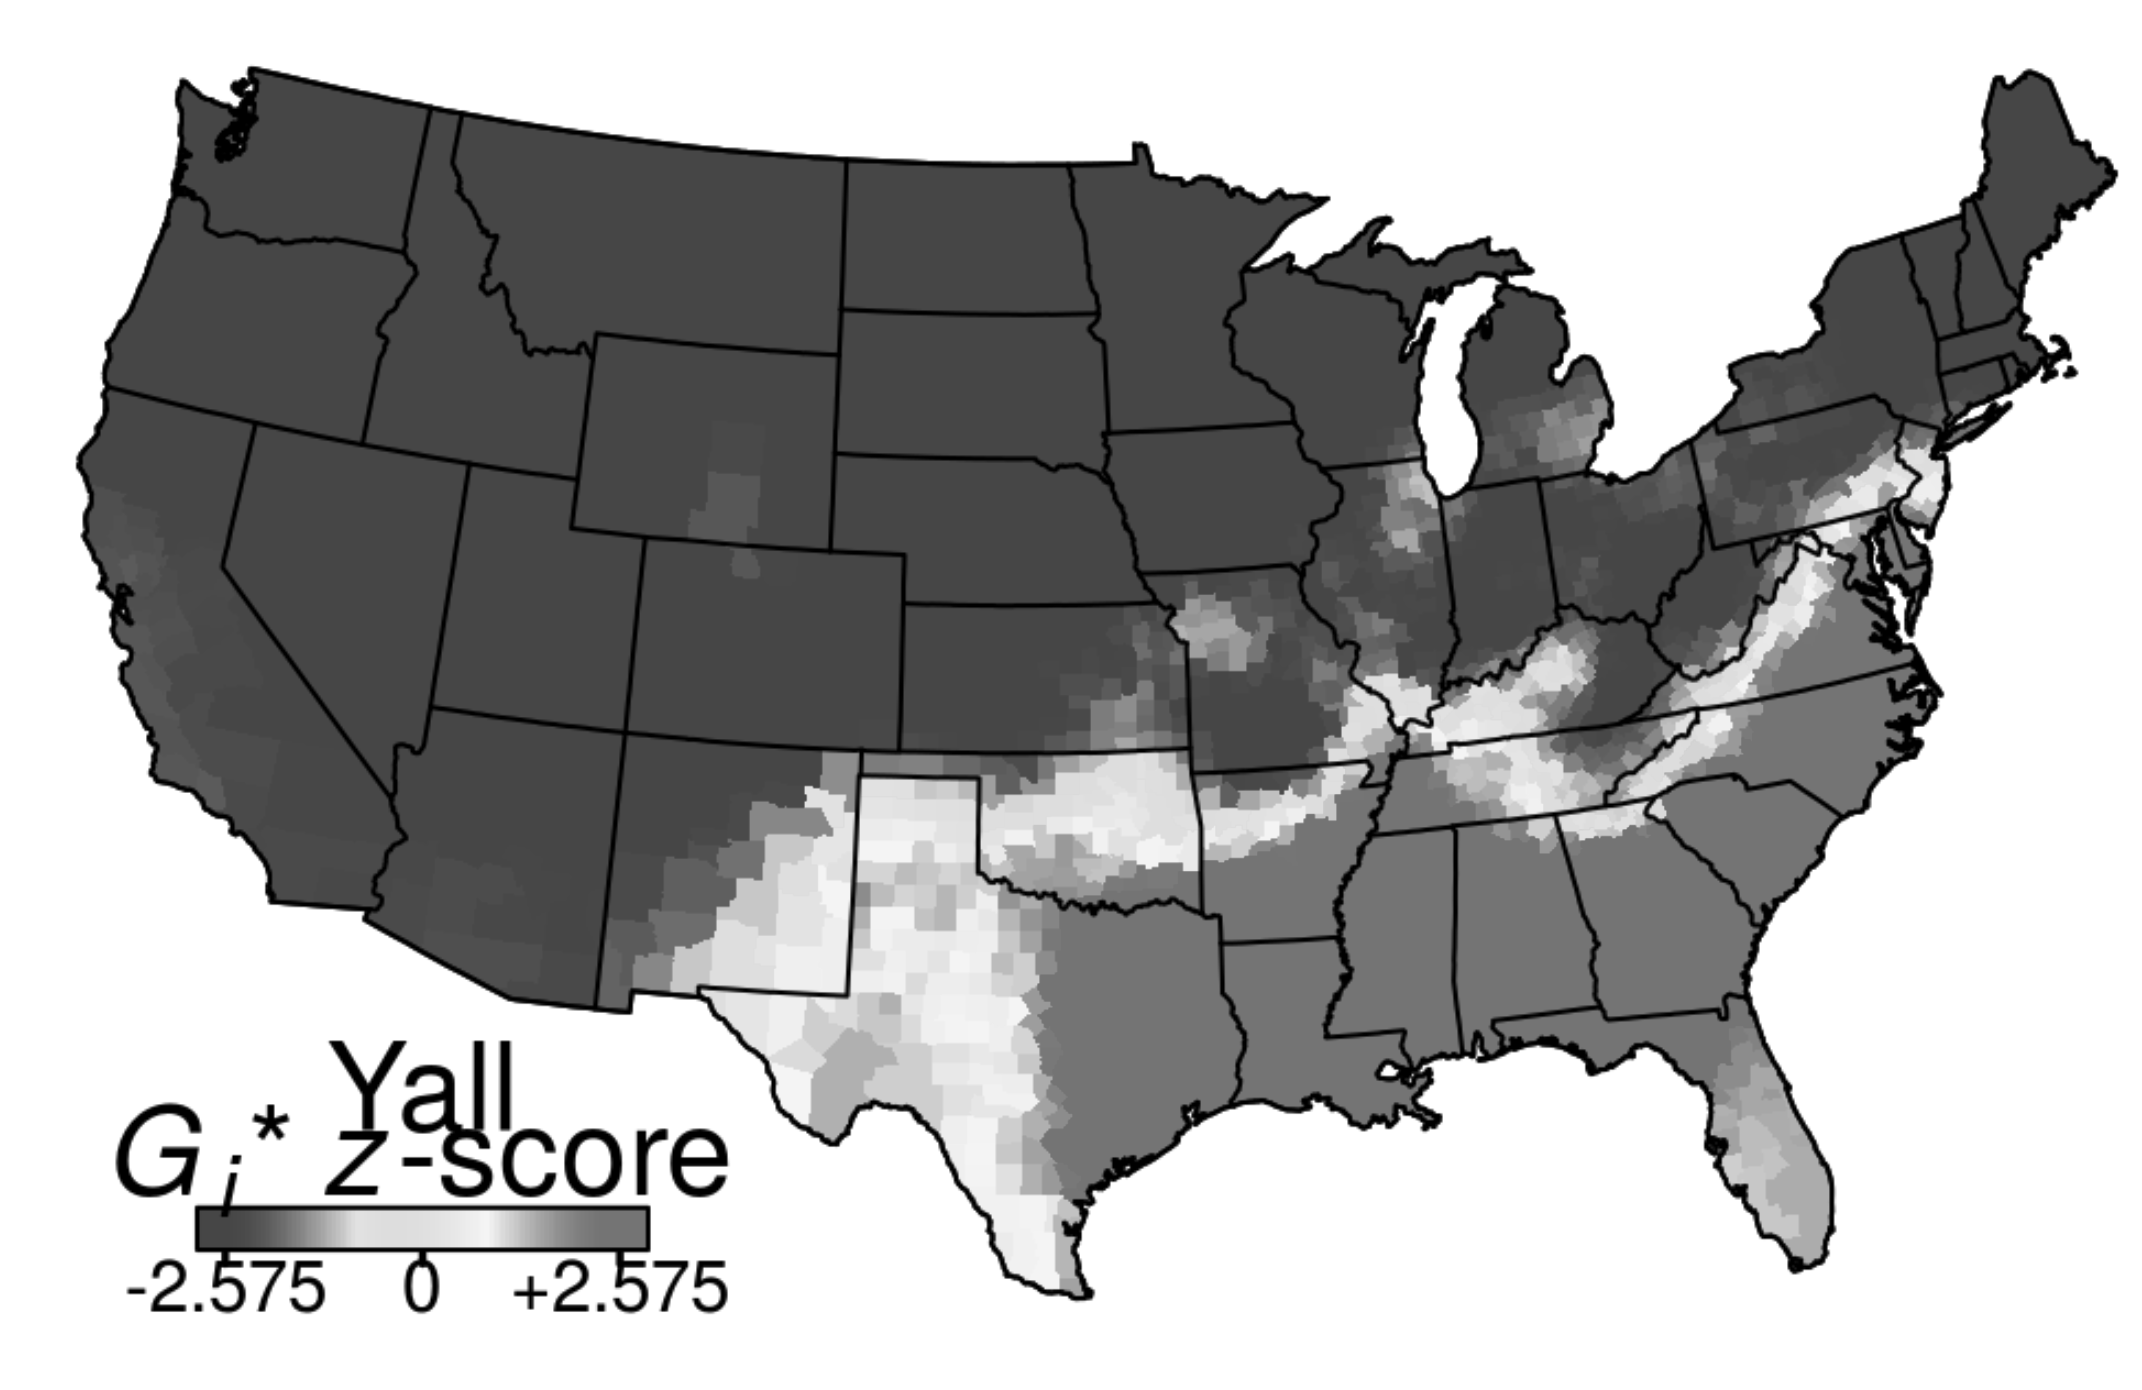
\includegraphics[width=1\textwidth,height=\textheight]{part_2/figures/data-word-mapper.png}

}

\caption{\label{fig-data-word-mapper}Example distribution of the term
``Yall'' the Word Mapper Project}

\end{figure}%

\end{minipage}%

\end{figure}%

\end{tcolorbox}

The more common measures for numeric variables are the mean and the
median. The \textbf{mean} is a summary statistic calculated by summing
all the values and dividing by the number of values. The \textbf{median}
is calculated by sorting all the values in the variable and then
selecting the middle value.

\begin{table}

\caption{\label{tbl-analysis-belc-central-tendency}Central tendency
measures for the BELC dataset}

\begin{minipage}{0.50\linewidth}

\subcaption{\label{tbl-analysis-belc-central-tendency-1}Categorical variables}

\centering{

\begin{tabular}{ll}
\toprule
variable & top\_counts\\
\midrule
essay\_id & E1: 1, E10: 1, E11: 1, E12: 1\\
part\_id & L05: 3, L10: 3, L11: 3, L12: 3\\
sex & fem: 48, mal: 32\\
group & T1: 25, T3: 24, T2: 16, T4: 15\\
\bottomrule
\end{tabular}

}

\end{minipage}%
%
\begin{minipage}{0.50\linewidth}

\subcaption{\label{tbl-analysis-belc-central-tendency-2}Numeric variables}

\centering{

\begin{tabular}{lll}
\toprule
variable & mean & median\\
\midrule
tokens & 67.62 & 56.5\\
types & 41.85 & 38.5\\
ttr & 0.68 & 0.66\\
prop\_l2 & 0.96 & 0.99\\
\bottomrule
\end{tabular}

}

\end{minipage}%

\end{table}%

As the mode is the most frequent value, the \texttt{top\_counts} measure
in Table~\ref{tbl-analysis-belc-central-tendency} provides the most
frequent value for the categorical variables. Mean and median appear but
we notice that the mean and median are not the same for the numeric
variables. Differences that appear between the mean and median will be
of interest to us later in this chapter.

\subsection{Dispersion}\label{dispersion}

To understand how representative a central tendency measure is we use a
calculation of the the spread of the values around the central tendency,
or \textbf{dispersion}. Dispersion is a measure of how spread out the
values are around the central tendency. The more spread out the values,
the less representative the central tendency measure is.

For categorical variables, the spread is framed in terms of how balanced
the values are across the levels. One way to do this is to use
proportions. The \textbf{proportion} of each level is the frequency of
the level divided by the total number of values. Another way is to
calculate the (normalized) entropy. \textbf{Entropy} is a single measure
of uncertainty. The more balanced the values are across the levels, the
closer entropy is 1. In practice, however, proportions are often used to
assess the balance of the values across the levels.

The most common measure of dispersion for numeric variables is the
\textbf{standard deviation}. The standard deviation is calculated by
taking the square root of the variance. The \textbf{variance} is the
average of the squared differences from the mean. So, more succinctly,
the standard deviation is a measure of the spread of the values around
the mean. Where the standard deviation is anchored to the mean, the
\textbf{interquartile range} (IQR) is tied to the median. The median
represents the sorted middle of the values, in other words the 50th
percentile. The IQR is the difference between the 75th percentile and
the 25th percentile.

\begin{table}

\caption{\label{tbl-analysis-belc-dispersion}Dispersion measures for the
BELC dataset}

\begin{minipage}{0.50\linewidth}

\subcaption{\label{tbl-analysis-belc-dispersion-1}Categorical variables}

\centering{

\begin{tabular}{ll}
\toprule
variable & norm\_entropy\\
\midrule
essay\_id & 1\\
part\_id & 0.98\\
sex & 0.97\\
group & 0.98\\
\bottomrule
\end{tabular}

}

\end{minipage}%
%
\begin{minipage}{0.50\linewidth}

\subcaption{\label{tbl-analysis-belc-dispersion-2}Numeric variables}

\centering{

\begin{tabular}{lll}
\toprule
variable & sd & iqr\\
\midrule
tokens & 44.2 & 61.25\\
types & 23.03 & 31.5\\
ttr & 0.13 & 0.149\\
prop\_l2 & 0.1 & 0.027\\
\bottomrule
\end{tabular}

}

\end{minipage}%

\end{table}%

\begin{tcolorbox}[enhanced jigsaw, left=2mm, toprule=.15mm, colback=white, colframe=quarto-callout-color-frame, arc=.35mm, rightrule=.15mm, bottomrule=.15mm, leftrule=.75mm, breakable, opacityback=0]

\textbf{\faIcon{medal} Dive deeper}

The inability to compare summary statistics across variables is a key
reason why \textbf{standardization} is often applied before submiting a
dataset for analysis (\citeproc{ref-Baayen2008a}{R. Harald Baayen,
2008}; \citeproc{ref-Johnson2008}{Johnson, 2008}).

Standardization is a scale-based transformation that changes the scale
of the values to a common scale, or \emph{z-scores}. The result of this
transformation puts data points of each variable on the same scale and
allows for direct comparison. Furthermore, standardization also
mitigates the influence of variables with large values relative to other
variables. This is particularly important in multivariate analysis where
the influence of variables with large values can be magnified.

The caveat is that standardization masks the original meaning of the
data. That is, if we consider token frequency, before standardization,
we can say that a value of 1000 tokens is 1000 tokens. After
standardization, we can only say that a value of 1 is 1 standard
deviation from the mean. This is why standardization is often applied
after the descriptive phase of analysis.

\end{tcolorbox}

In Table~\ref{tbl-analysis-belc-dispersion-1}, the normalized entropy
helps us understand the balance of the values across the levels of the
categorical variables. In Table~\ref{tbl-analysis-belc-dispersion-2},
the standard deviation and IQR provide a sense of the spread of the
values around the mean and median, respectively, for the numeric
variables.

When interpreting numeric central tendency and dispersion values, it is
important to only directly compare column-wise. That is, focusing only
on a single variable, not across variables. Each variable, as is, is
measured on a different scale and only relative to itself can we make
sense of the values.

\subsection{Distributions}\label{sec-analysis-distributions}

Summary statistics of the central tendency and dispersion of a variable
provide a sense of the most representative value and how spread out the
data is around this value. However, to gain a more comprehensive
understanding of the variable, it is key to consider the frequencies of
all the data points. The \textbf{distribution} of a variable is the
pattern or shape of the data that emerges when the frequencies of all
data points are considered. This can reveal patterns that might not be
immediately apparent from summary statistics alone.

When assessing the distribution of categorical variables, we can use a
frequency table or bar plot. \textbf{Frequency tables} display the
frequency and/ or proportion each level in a categorical variable in a
clear and concise manner. In
Table~\ref{tbl-analysis-belc-frequency-table} we see the frequency table
for the variable \texttt{sex} and \texttt{group}.

\begin{table}

\caption{\label{tbl-analysis-belc-frequency-table}Frequency table for
variables in the BELC dataset}

\begin{minipage}{0.50\linewidth}

\subcaption{\label{tbl-analysis-belc-frequency-table-1}Sex}

\centering{

\begin{tabular}{lll}
\toprule
sex & frequency & proportion\\
\midrule
female & 48 & 0.6\\
male & 32 & 0.4\\
\bottomrule
\end{tabular}

}

\end{minipage}%
%
\begin{minipage}{0.50\linewidth}

\subcaption{\label{tbl-analysis-belc-frequency-table-2}Time group}

\centering{

\begin{tabular}{lll}
\toprule
group & frequency & proportion\\
\midrule
T1 & 25 & 0.312\\
T2 & 16 & 0.200\\
T3 & 24 & 0.300\\
T4 & 15 & 0.188\\
\bottomrule
\end{tabular}

}

\end{minipage}%

\end{table}%

A \textbf{bar plot} is a type of plot where the x-axis is a categorical
variable and the y-axis is the frequency of the values. The frequency is
represented by the height of the bar. The variables can be ordered by
frequency, alphabetically, or some other order.
Figure~\ref{fig-analysis-belc-barplots} is a bar chart for the variables
\texttt{sex} and \texttt{group} ordered alphabetically.

\begin{figure}[!htb]

\begin{minipage}{0.50\linewidth}

\centering{

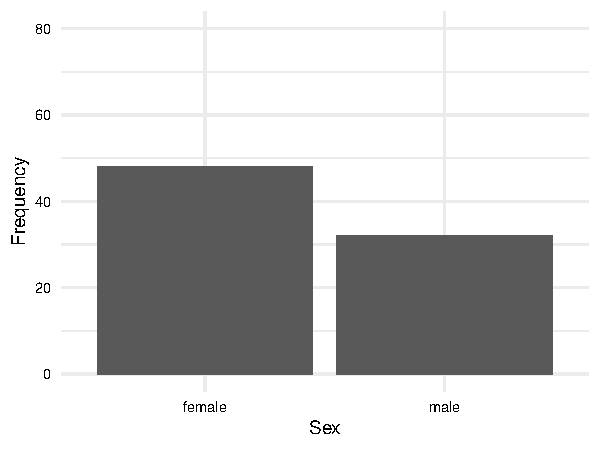
\includegraphics{part_2/3_analysis_files/figure-pdf/fig-analysis-belc-barplots-1.pdf}

}

\subcaption{\label{fig-analysis-belc-barplots-1}Bar plot}

\end{minipage}%
%
\begin{minipage}{0.50\linewidth}

\centering{

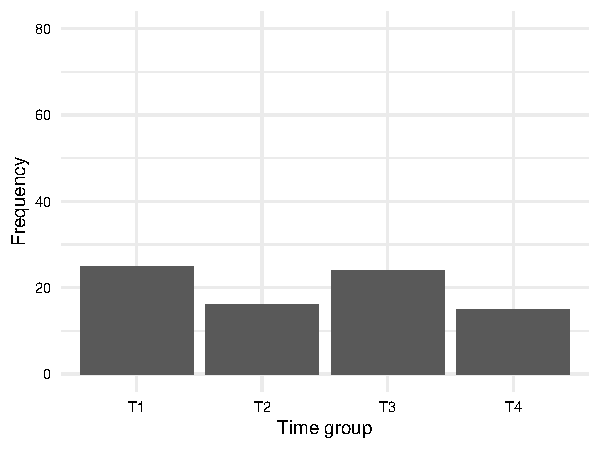
\includegraphics{part_2/3_analysis_files/figure-pdf/fig-analysis-belc-barplots-2.pdf}

}

\subcaption{\label{fig-analysis-belc-barplots-2}Bar plot}

\end{minipage}%

\caption{\label{fig-analysis-belc-barplots}Bar plots for categorical
variables \texttt{sex} and \texttt{group}}

\end{figure}%

So for a frequency table or barplot, we can see the frequency of each
level of a categorical variable. This gives us some knowledge about the
BELC dataset: there are more girls in the dataset and more essays appear
in first and third time groups. If we were to see any clearly loopsided
categories, this would be a sign of imbalance in the data and we would
need to consider how this might impact our analysis.

\begin{tcolorbox}[enhanced jigsaw, left=2mm, toprule=.15mm, colback=white, colframe=quarto-callout-color-frame, arc=.35mm, rightrule=.15mm, bottomrule=.15mm, leftrule=.75mm, breakable, opacityback=0]

\textbf{\faIcon{lightbulb} Consider this}

The goal of descriptive statistics is to summarize the data in a way
that is meaningful and interpretable. With this in mind, compare the
frequency tables in \ref{tbl-analysis-belc-frequency-table} and bar
plots in \ref{fig-analysis-belc-barplots}. Does one provide a more
interpretable summary of the data? Why or why not? Are there any other
ways you might communicate this distribution more effectively?

\end{tcolorbox}

Numeric variables are best understood visually. The most common
visualizations of the distribution of a numeric variable are histograms
and density plots. \textbf{Histograms} are a type of bar plot where the
x-axis is a numeric variable and the y-axis is the frequency of the
values falling within a determined range of values, or bins. The
frequency of values within each bin is represented by the height of the
bars.

\textbf{Density plots} are a smoothed version of histograms. The y-axis
of a density plot is the probability of the values. When frequent values
appear closely together, the plot line is higher. When the frequency of
values is lower or more spread out, the plot line is lower.

\begin{figure}[!htb]

\begin{minipage}{0.50\linewidth}

\centering{

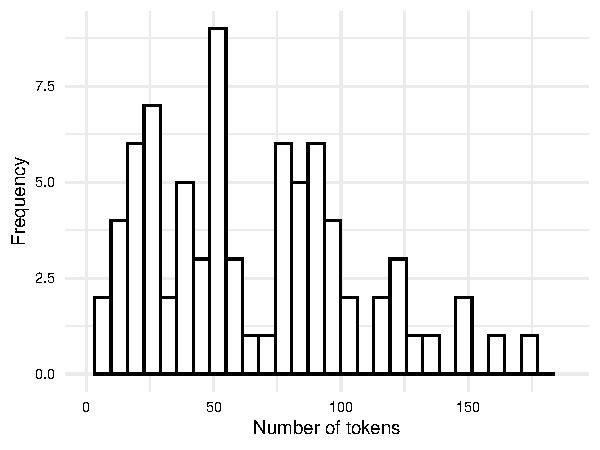
\includegraphics{part_2/3_analysis_files/figure-pdf/fig-analysis-belc-histogram-density-tokens-1.pdf}

}

\subcaption{\label{fig-analysis-belc-histogram-density-tokens-1}Histogram}

\end{minipage}%
%
\begin{minipage}{0.50\linewidth}

\centering{

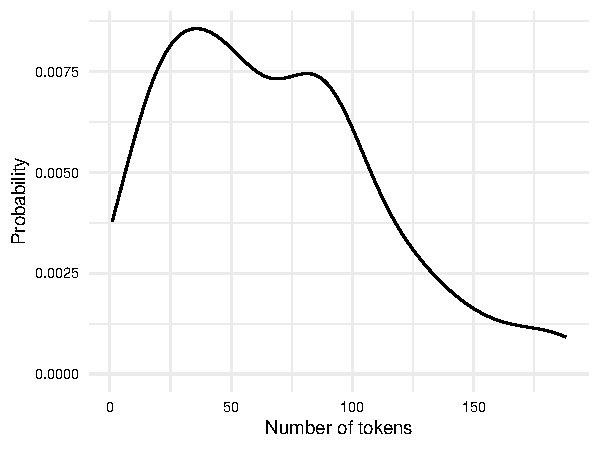
\includegraphics{part_2/3_analysis_files/figure-pdf/fig-analysis-belc-histogram-density-tokens-2.pdf}

}

\subcaption{\label{fig-analysis-belc-histogram-density-tokens-2}Density
plot}

\end{minipage}%

\caption{\label{fig-analysis-belc-histogram-density-tokens}Distribution
plots for the variable \texttt{tokens}.}

\end{figure}%

Both the histogram in
Figure~\ref{fig-analysis-belc-histogram-density-tokens-1} and the
density plot in
Figure~\ref{fig-analysis-belc-histogram-density-tokens-2} show the
distribution of the variable \texttt{tokens} in slightly different ways
which translate into trade-offs in terms of interpretability.

The histogram shows the frequency of the values in bins. The number of
bins and/ or binwidth can be changed for more or less granularity. A
rough grain histogram shows the general shape of the distribution, but
it is difficult to see the details of the distribution. A fine grain
histogram shows the details of the distribution, but it is difficult to
see the general shape of the distribution. The density plot shows the
general shape of the distribution, but it hides the details of the
distribution. Given this trade-off, it is often useful explore outliers
with histograms and the overall shape of the distribution with density
plots.

\begin{figure}[!htb]

\begin{minipage}{0.33\linewidth}

\centering{

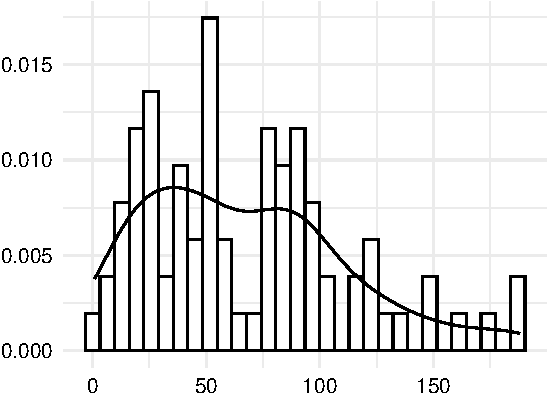
\includegraphics{part_2/3_analysis_files/figure-pdf/fig-analysis-belc-histograms-1.pdf}

}

\subcaption{\label{fig-analysis-belc-histograms-1}Number of tokens}

\end{minipage}%
%
\begin{minipage}{0.33\linewidth}

\centering{

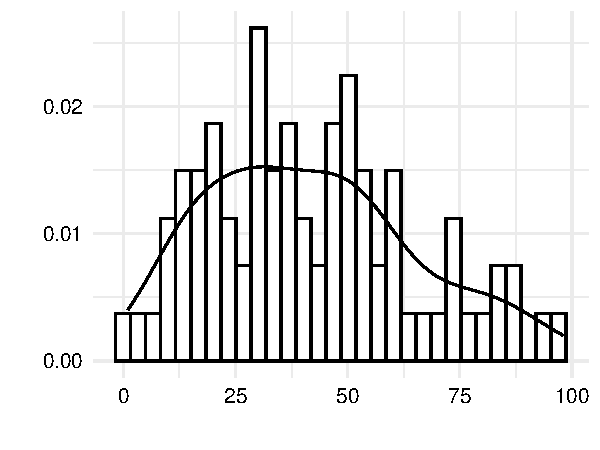
\includegraphics{part_2/3_analysis_files/figure-pdf/fig-analysis-belc-histograms-2.pdf}

}

\subcaption{\label{fig-analysis-belc-histograms-2}Number of types}

\end{minipage}%
%
\begin{minipage}{0.33\linewidth}

\centering{

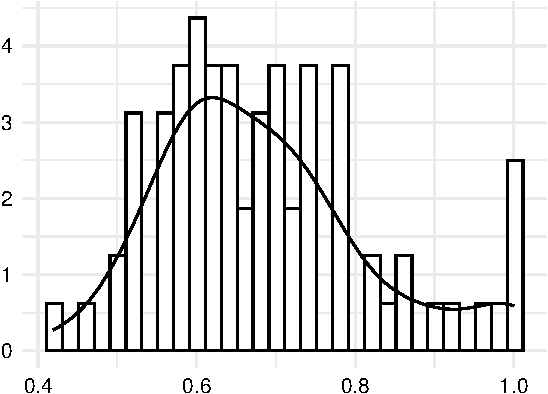
\includegraphics{part_2/3_analysis_files/figure-pdf/fig-analysis-belc-histograms-3.pdf}

}

\subcaption{\label{fig-analysis-belc-histograms-3}Type-token ratio
score}

\end{minipage}%

\caption{\label{fig-analysis-belc-histograms}Histograms for numeric
variables \texttt{tokens}, \texttt{types}, and \texttt{ttr}.}

\end{figure}%

In Figure~\ref{fig-analysis-belc-histograms} we see both histograms and
density plots combined for the variables \texttt{tokens},
\texttt{types}, and \texttt{ttr}. Focusing on the details captured in
the histogram we are better able to detect potential outliers. Outliers
can reflect valid values that are simply extreme or they can reflect
something erroneous in the data. To distinguish between these two
possibilities, it is important to know the context of the data. Take,
for example, Figure~\ref{fig-analysis-belc-histograms-3}. We see that
there is a bin near the value 1.0. Given that the type-token ratio is a
ratio of the number of types to the number of tokens, it is unlikely
that the type-token ratio would be exactly 1.0 as this would mean that
every word in an essay is unique. Another, less dramatic, example is the
bin to the far right of Figure~\ref{fig-analysis-belc-histograms-1}. In
this case, the bin represents the number of tokens in an essay. An
uptick in the number of essays with a large number of tokens is not
surprising and would not typically be considered an outlier. On the
other hand, consider the bin near the value 0 in the same plot. It is
unlikely that a true essay would have 0, or near 0, words and therefore
a closer look at the data is warranted.

It is important to recognize that outliers contribute undue influence to
overall measures of central tendency and dispersion. To appreciate this,
let's consider another helpful visualization called a \textbf{boxplot}.
A boxplot is a visual representation which aims to represent the central
tendency, dispersion, and distribution of a numeric variable in one
plot.

\begin{figure}[!htb]

\begin{minipage}{\linewidth}

\centering{

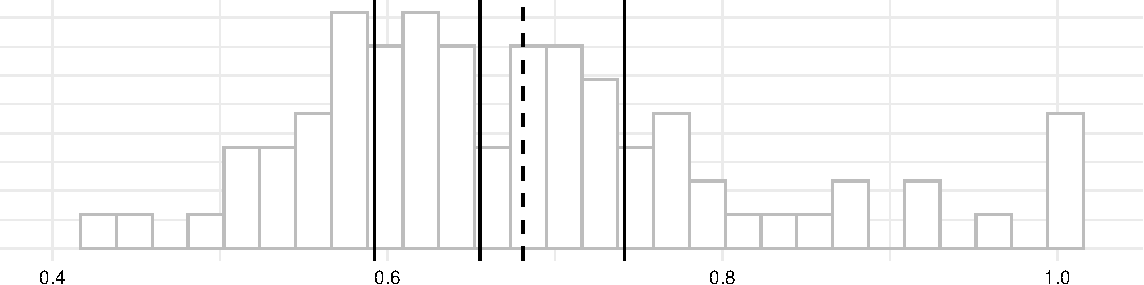
\includegraphics{part_2/3_analysis_files/figure-pdf/fig-analysis-belc-histogram-boxplot-1.pdf}

}

\subcaption{\label{fig-analysis-belc-histogram-boxplot-1}Histogram}

\end{minipage}%
\newline
\begin{minipage}{\linewidth}

\centering{

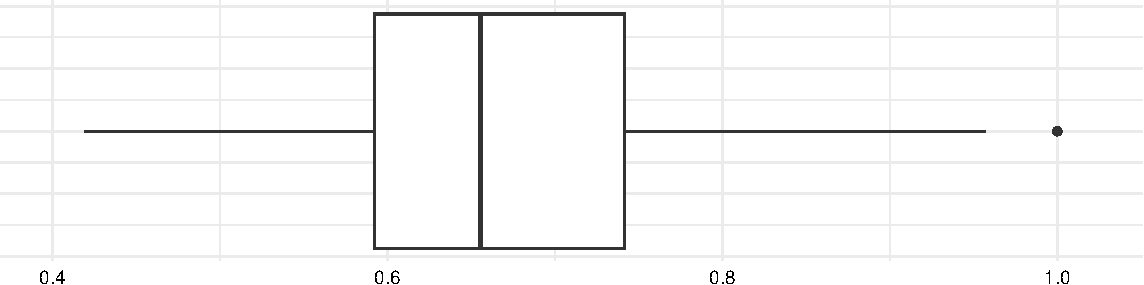
\includegraphics{part_2/3_analysis_files/figure-pdf/fig-analysis-belc-histogram-boxplot-2.pdf}

}

\subcaption{\label{fig-analysis-belc-histogram-boxplot-2}Boxplot}

\end{minipage}%

\caption{\label{fig-analysis-belc-histogram-boxplot}Understanding the
similarities between boxplots and histograms}

\end{figure}%

In Figure~\ref{fig-analysis-belc-histogram-boxplot-2} we see a boxplot
for \texttt{ttr} variable. The box in the middle of the plot represents
the interquartile range (IQR) which is the range of values between the
first quartile and the third quartile. The solid line in the middle of
the box represents the median. The lines extending from the box are
called `whiskers' and provide the range of values which are within 1.5
times the IQR. Values outside of this range are plotted as individual
points.

Now let's consider boxplots from another angle. Just above in
Figure~\ref{fig-analysis-belc-histogram-boxplot-1} I've plotted a
histogram. In this view, we can see that a boxplot is a simplifed
histogram augmented with central tendency and dispersion statistics.
While histograms focus on the frequency distribution of data points,
boxplots focus on the data's quartiles and potential outliers.

Concerning outliers, it is important to address them to safeguard the
accuracy of the analysis. There are two main ways to address outliers:
eliminate observations with outliers or transform the data. The
elimination, or \textbf{trimming}, of outliers is more extreme as it
removes data but can be the best approach for true outliers.
Transforming the data is an approach to mitigating the influence of
extreme but valid values. \textbf{Transformation} involves applying a
mathematical function to the data which changes the scale and/ or shape
of the distribution, but does not remove data nor does it change the
relative order of the values.

The exploration the data points with histograms and boxplots has helped
us to identify outliers. Now we turn to the question of the overall
shape of the distribution.

When values are symmetrically dispersed around the central tendency, the
distribution is said to be normal. The \textbf{Normal Distribution} is
characterized by a distribution where the mean and median are the same.
The Normal Distribution has a key role in theoretical statistics and is
the foundation for many statistical tests. This distribution is also
known as the Gaussian Distribution or the Bell Curve for the hallmark
bell shape of the distribution. In a normal distribution, extreme values
are less likely than values near the center.

When values are not symmetrically dispersed around the central tendency,
the distribution is said to be skewed. A distribution in which values
tend to disperse to the left of the central tendency is \textbf{left
skewed} and a distribution in which values tend to disperse to the right
of the central tendency is \textbf{right skewed}.

Simulations of these distributions appear in
Figure~\ref{fig-analysis-distributions}.

\begin{figure}[!htb]

\begin{minipage}{0.33\linewidth}

\centering{

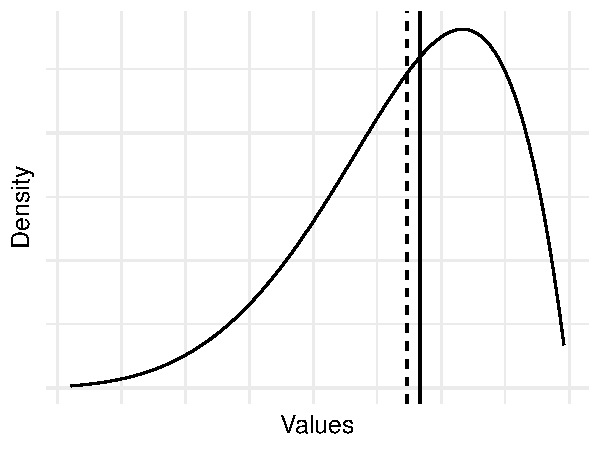
\includegraphics{part_2/3_analysis_files/figure-pdf/fig-analysis-distributions-1.pdf}

}

\subcaption{\label{fig-analysis-distributions-1}Left-skewed}

\end{minipage}%
%
\begin{minipage}{0.33\linewidth}

\centering{

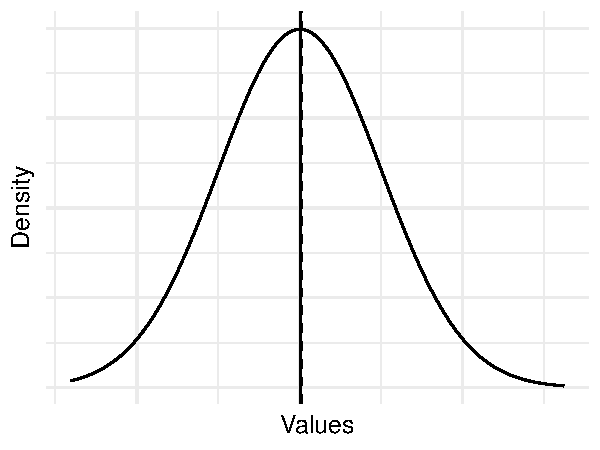
\includegraphics{part_2/3_analysis_files/figure-pdf/fig-analysis-distributions-2.pdf}

}

\subcaption{\label{fig-analysis-distributions-2}Normal}

\end{minipage}%
%
\begin{minipage}{0.33\linewidth}

\centering{

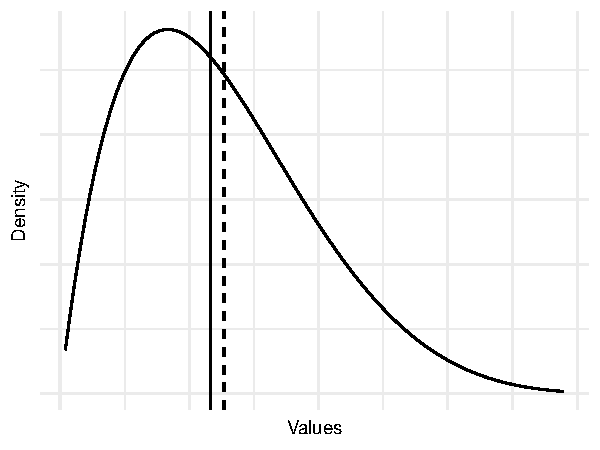
\includegraphics{part_2/3_analysis_files/figure-pdf/fig-analysis-distributions-3.pdf}

}

\subcaption{\label{fig-analysis-distributions-3}Right-skewed}

\end{minipage}%

\caption{\label{fig-analysis-distributions}Mean and median for normal
and skewed distributions}

\end{figure}%

Assessing the distribution of a variable is important for two reasons.
First, the distribution of a variable can inform the choice of
statistical test in theory-based hypothesis testing. Data that are
normally, or near-normally distributed are often analyzed using
parametric tests while data that exhibit a skewed distributed are often
analyzed using non-parametric tests. Second, highly skewed distributions
have the effect of compressing the range of values. This can lead to a
loss of information and can make it difficult to detect patterns in the
data.

Skewed frequency distributions are commonly found for linguistic units
(\emph{.e.g} phonemes, morphemes, words, \emph{etc.}). However, these
distributions tend to a follow a particular type of skew known as a Zipf
distribution. According to \textbf{Zipf's Law}
(\citeproc{ref-Zipf1949}{Zipf, 1949}), the frequency of a linguistic
unit is inversely proportional to its rank. In other words, the most
frequent units will appear twice as often as the second most frequent
unit, three times as often as the third most frequent unit, and so on.

The plot in Figure~\ref{fig-analysis-zipf-distribution-1} is simulated
data that fits a Zipfian distribution.

\begin{figure}[!htb]

\begin{minipage}{0.50\linewidth}

\centering{

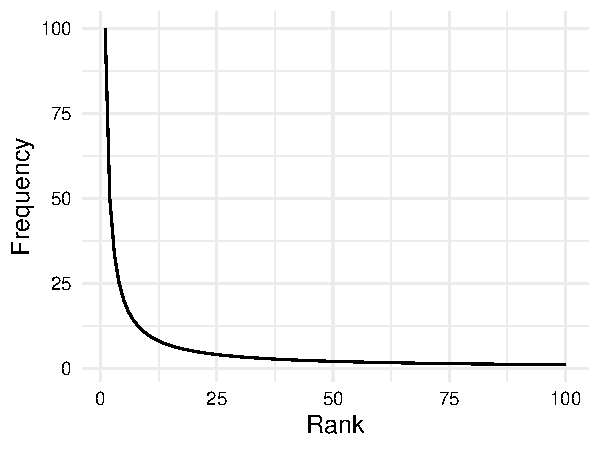
\includegraphics{part_2/3_analysis_files/figure-pdf/fig-analysis-zipf-distribution-1.pdf}

}

\subcaption{\label{fig-analysis-zipf-distribution-1}Zipfian
distribution}

\end{minipage}%
%
\begin{minipage}{0.50\linewidth}

\centering{

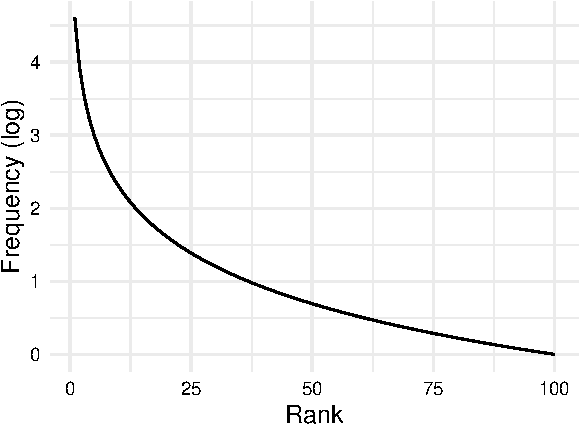
\includegraphics{part_2/3_analysis_files/figure-pdf/fig-analysis-zipf-distribution-2.pdf}

}

\subcaption{\label{fig-analysis-zipf-distribution-2}Log-transformed
Zipfian distribution}

\end{minipage}%

\caption{\label{fig-analysis-zipf-distribution}Zipfian distribution}

\end{figure}%

Zipf's law describes a theoretical distribution, and the actual
distribution of units in a corpus is affected by various sampling
factors, including the size of the corpus. The larger the corpus, the
closer the distribution will be to the Zipf distribution.

\begin{tcolorbox}[enhanced jigsaw, left=2mm, toprule=.15mm, colback=white, colframe=quarto-callout-color-frame, arc=.35mm, rightrule=.15mm, bottomrule=.15mm, leftrule=.75mm, breakable, opacityback=0]

\textbf{\faIcon{medal} Dive deeper}

As stated above, Zipfian distributions are typical of natural language
and are observed a various linguistic levels. This is because natural
language is a complex system, and complex systems tend to exhibit
Zipfian distributions. Other examples of complex systems that exhibit
Zipfian distributions include the size of cities, the frequency of
species in ecological communities, the frequency of links in the World
Wide Web, \emph{etc.}

\end{tcolorbox}

In the case that a variable is highly skewed (such as in linguistic
frequency distributions), it is often useful to attempt transform the
variable to reduce the skewness. In contrast to scale-based
transformations (\emph{e.g.} centering and scaling), shape-based
transformations change the scale and the shape of the distribution. The
most common shape-based transformation is the logarithmic
transformation. The \textbf{logarithmic transformation}
(log-transformation) takes the log (typically base 10) of each value in
a variable. The log-transformation is useful for reducing the skewness
of a variable as it compresses large values and expands small values. If
the skewness is due to these factors, the log-transformation can help,
as in the case of the Zipfian distribution in
Figure~\ref{fig-analysis-zipf-distribution-2}.

It is important to note, however, that if scale-based transformations
are to be applied to a variable, they should be applied after the
log-transformation as the log of negative values is undefined.

\subsection{Association}\label{association}

We have covered the first three of the four questions we are interested
in asking in a descriptive analysis. The fourth, and last, question is
whether there is an association between variables. If so, what is the
directionality and what is the apparent magnitude of the dependence?
Knowing the answers to these questions will help frame our approach to
analysis.

To assess association, the number and information types of the variables
under consideration are important. Let's start by considering two
variables. If we are working with two variables, we are dealing with a
\textbf{bivariate} relationship. Given there are three informational
types (categorical, ordinal, and numeric), there are six logical
bivariate combinations: categorical-categorical, categorical-ordinal,
categorical-numeric, ordinal-ordinal, ordinal-numeric, and
numeric-numeric.

The directionality of a relationship will take the form of a tabular or
graphic summary depending on the informational value of the variables
involved. In Table~\ref{tbl-analysis-summary-types}, we see the
appropriate summary types for each of the six bivariate combinations.

\begin{longtable}[]{@{}
  >{\raggedright\arraybackslash}p{(\columnwidth - 6\tabcolsep) * \real{0.1700}}
  >{\raggedright\arraybackslash}p{(\columnwidth - 6\tabcolsep) * \real{0.2700}}
  >{\raggedright\arraybackslash}p{(\columnwidth - 6\tabcolsep) * \real{0.2800}}
  >{\raggedright\arraybackslash}p{(\columnwidth - 6\tabcolsep) * \real{0.2800}}@{}}
\caption{Appropriate summary types for different combinations of
variable types}\label{tbl-analysis-summary-types}\tabularnewline
\toprule\noalign{}
\begin{minipage}[b]{\linewidth}\raggedright
\end{minipage} & \begin{minipage}[b]{\linewidth}\raggedright
Categorical
\end{minipage} & \begin{minipage}[b]{\linewidth}\raggedright
Ordinal
\end{minipage} & \begin{minipage}[b]{\linewidth}\raggedright
Numeric
\end{minipage} \\
\midrule\noalign{}
\endfirsthead
\toprule\noalign{}
\begin{minipage}[b]{\linewidth}\raggedright
\end{minipage} & \begin{minipage}[b]{\linewidth}\raggedright
Categorical
\end{minipage} & \begin{minipage}[b]{\linewidth}\raggedright
Ordinal
\end{minipage} & \begin{minipage}[b]{\linewidth}\raggedright
Numeric
\end{minipage} \\
\midrule\noalign{}
\endhead
\bottomrule\noalign{}
\endlastfoot
\textbf{Categorical} & Contingency table & Contingency table/ Bar plot &
Pivot table/ Boxplot \\
\textbf{Ordinal} & - & Contingency table/ Bar plot & Pivot table/
Boxplot \\
\textbf{Numeric} & - & - & Scatterplot \\
\end{longtable}

Let's first start with the combinations that include a categorical or
ordinal variable. Categorical and ordinal variables reflect measures of
class-type information, with add meaningful ranks to ordinal variables.
To assess a relationship with these variable types, a table is always a
good place to start. When combined together, a contingency table is the
appropriate table. A \textbf{contingency table} is a cross-tabulation of
two class-type variables, basically a two-way frequency table. This
means that three of the six bivariate combinations are assessed with a
contingency table: categorical-categorical, categorical-ordinal, and
ordinal-ordinal.

In Table~\ref{tbl-analysis-belc-contingency-tables} we see contingency
tables for the categorical variable \texttt{sex} and ordinal variable
\texttt{group} in the BELC dataset. A contingency table may include only
counts, as in Table~\ref{tbl-analysis-belc-contingency-tables-1}, or may
include proportions or percentages in an effort to normalize the counts
and make them more comparable, as in
Table~\ref{tbl-analysis-belc-contingency-tables-2}.

\begin{table}

\caption{\label{tbl-analysis-belc-contingency-tables}Contingency tables
for categorical variable \texttt{sex} and ordinal variable
\texttt{group} in the BELC dataset}

\begin{minipage}{0.50\linewidth}

\subcaption{\label{tbl-analysis-belc-contingency-tables-1}Counts}

\centering{

\begin{tabular}{llll}
\toprule
group & female & male & Total\\
\midrule
T1 & 14 & 11 & 25\\
T2 & 11 & 5 & 16\\
T3 & 13 & 11 & 24\\
T4 & 10 & 5 & 15\\
Total & 48 & 32 & 80\\
\bottomrule
\end{tabular}

}

\end{minipage}%
%
\begin{minipage}{0.50\linewidth}

\subcaption{\label{tbl-analysis-belc-contingency-tables-2}Percentages}

\centering{

\begin{tabular}{llll}
\toprule
group & female & male & Total\\
\midrule
T1 & 56.00\% & 44.00\% & 100.00\%\\
T2 & 68.75\% & 31.25\% & 100.00\%\\
T3 & 54.17\% & 45.83\% & 100.00\%\\
T4 & 66.67\% & 33.33\% & 100.00\%\\
Total & 60.00\% & 40.00\% & 100.00\%\\
\bottomrule
\end{tabular}

}

\end{minipage}%

\end{table}%

It is sometimes helpful to visualize a contingency table as a bar plot
when there are a larger number of levels in either or both of the
variables. Again, looking at the relationship between \texttt{sex} and
\texttt{group}, we see that we can plot the counts or the proportions.
In Figure~\ref{fig-analysis-belc-bar-plots}, we see both.

\begin{figure}[!htb]

\begin{minipage}{0.50\linewidth}

\centering{

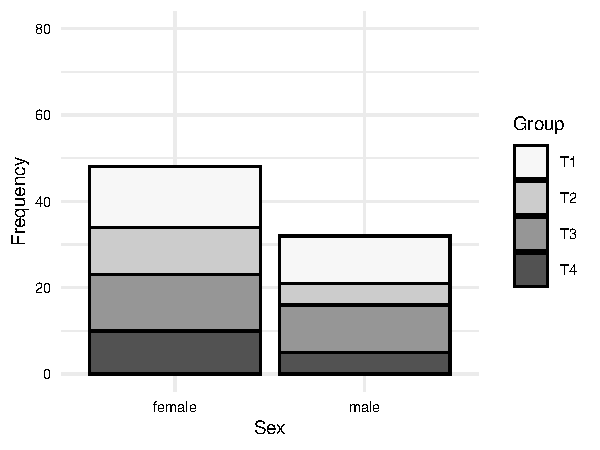
\includegraphics{part_2/3_analysis_files/figure-pdf/fig-analysis-belc-bar-plots-1.pdf}

}

\subcaption{\label{fig-analysis-belc-bar-plots-1}Counts}

\end{minipage}%
%
\begin{minipage}{0.50\linewidth}

\centering{

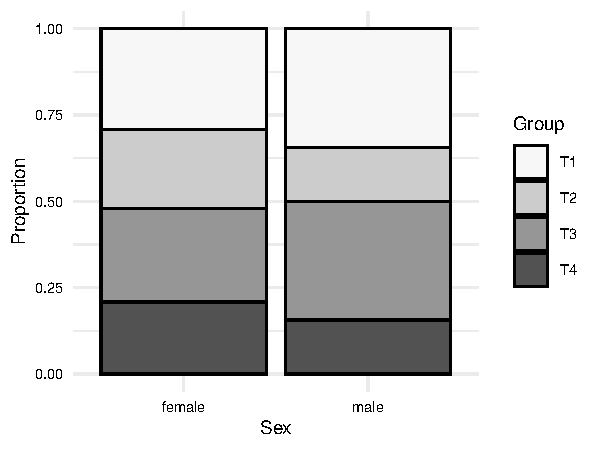
\includegraphics{part_2/3_analysis_files/figure-pdf/fig-analysis-belc-bar-plots-2.pdf}

}

\subcaption{\label{fig-analysis-belc-bar-plots-2}Proportions}

\end{minipage}%

\caption{\label{fig-analysis-belc-bar-plots}Bar plots for the
relationship between \texttt{sex} and \texttt{group} in the BELC
dataset}

\end{figure}%

To summarize and assess the relationship between a categorical or an
ordinal variable and a numeric variable, we cannot use a contingency
table. Instead, this type of relationship is best summarized in a table
using a summary statistic in a \textbf{pivot table}. A pivot table is a
table in which a class-type variable is used to group a numeric variable
by some summary statistic appropriate for numeric variables, \emph{e.g.}
mean, median, standard deviation, \emph{etc.}

In Table~\ref{tbl-analysis-belc-pivot-table}, we see a pivot table for
the relationship between \texttt{group} and \texttt{tokens} in the BELC
dataset. Specifically, we see the mean number of tokens by group. We see
that the mean number of tokens increases from Group T1 to T4, which is
consistent with the idea that the students in the higher groups are
writing longer essays.

\begin{longtable}[]{@{}
  >{\raggedright\arraybackslash}p{(\columnwidth - 2\tabcolsep) * \real{0.5000}}
  >{\raggedright\arraybackslash}p{(\columnwidth - 2\tabcolsep) * \real{0.5000}}@{}}

\caption{\label{tbl-analysis-belc-pivot-table}Pivot table for the mean
\texttt{tokens} by \texttt{group} in the BELC dataset}

\tabularnewline

\toprule\noalign{}
\begin{minipage}[b]{\linewidth}\raggedright
group
\end{minipage} & \begin{minipage}[b]{\linewidth}\raggedright
mean\_tokens
\end{minipage} \\
\midrule\noalign{}
\endhead
\bottomrule\noalign{}
\endlastfoot
T1 & 29.6 \\
T2 & 58.7 \\
T3 & 83.9 \\
T4 & 114.5 \\

\end{longtable}

Although a pivot table may be appropriate for targeted numeric
summaries, a visualization is often more informative for assessing the
dispersion and distribution of a numeric variable by a categorical or
ordinal variable. There are two main types of visualizations for this
type of relationship: a boxplot and a \textbf{violin plot}. A violin
plot is a visualization that summarizes the distribution of a numeric
variable by a categorical or ordinal variable, adding the overall shape
of the distribution, much as a density plot does for histograms.

In Figure~\ref{fig-analysis-belc-boxplot-violin-plot}, we see both a
boxplot and a violin plot for the relationship between \texttt{group}
and \texttt{tokens} in the BELC dataset. From the boxplot in
Figure~\ref{fig-analysis-belc-boxplot-violin-plot-1}, we see that the
general trend towards more tokens used by students in higher groups. But
we can also appreciate the dispersion of the data within each group
looking at the boxes and whiskers. On the surface it appears that the
data for groups T1 and T3 are closer to each other than groups T2 and
T4, in which there is more variability within these groups. Furthermore,
we can see outliers in groups T1 and T3, but not in groups T2 and T4.
From the violin plot in
Figure~\ref{fig-analysis-belc-boxplot-violin-plot-2}, we can see the
same information, but we can also see the overall shape of the
distribution of tokens within each group. In this plot, it is very clear
that group T4 includes a wide range of token counts.

\begin{figure}[!htb]

\begin{minipage}{0.50\linewidth}

\centering{

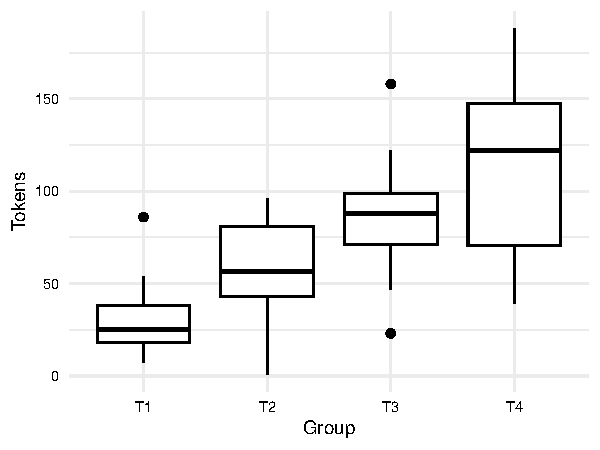
\includegraphics{part_2/3_analysis_files/figure-pdf/fig-analysis-belc-boxplot-violin-plot-1.pdf}

}

\subcaption{\label{fig-analysis-belc-boxplot-violin-plot-1}Boxplot}

\end{minipage}%
%
\begin{minipage}{0.50\linewidth}

\centering{

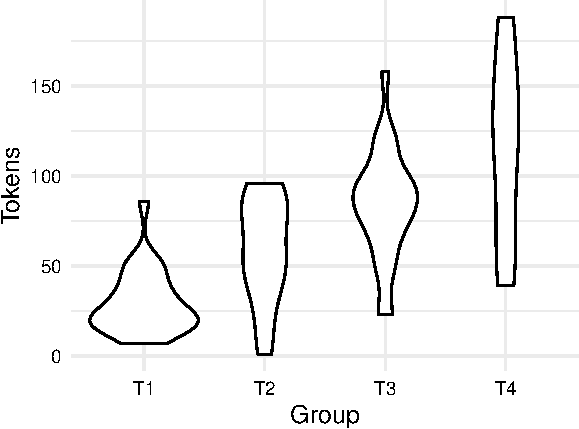
\includegraphics{part_2/3_analysis_files/figure-pdf/fig-analysis-belc-boxplot-violin-plot-2.pdf}

}

\subcaption{\label{fig-analysis-belc-boxplot-violin-plot-2}Violin plot}

\end{minipage}%

\caption{\label{fig-analysis-belc-boxplot-violin-plot}Boxplot and violin
plot for the relationship between \texttt{group} and \texttt{tokens} in
the BELC dataset}

\end{figure}%

The last bivariate combination is numeric-numeric. To summarize this
type of relationship a scatterplot is used. A \textbf{scatterplot} is a
visualization that plots each data point as a point in a two-dimensional
space, with one numeric variable on the x-axis and the other numeric
variable on the y-axis. Depending on the type of relationship you are
trying to assess, you may want to add a trend line to the scatterplot. A
trend line is a line that summarizes the overall trend in the
relationship between the two numeric variables. To assess the extent to
which the relationship is linear, a straight line is drawn which
minimizes the distance between the line and the points.

In Figure~\ref{fig-analysis-belc-scatter-plot}, we see a scatterplot and
a scatterplot with a trend line for the relationship between
\texttt{ttr} and \texttt{types} in the BELC dataset. We see that there
is an apparent positive relationship between these two variables, which
is consistent with the idea that as the number of types increases, the
type-token ratio increases. In other words, as the number of unique
words increases, so does the lexical diversity of the text. Since we are
evaluating a linear relationship, we are assessing the extent to which
there is a \textbf{correlation} between \texttt{ttr} and \texttt{types}.
A correlation simply means that as the values of one variable change,
the values of the other variable change in a consistent manner.

\begin{figure}[!htb]

\begin{minipage}{0.50\linewidth}

\centering{

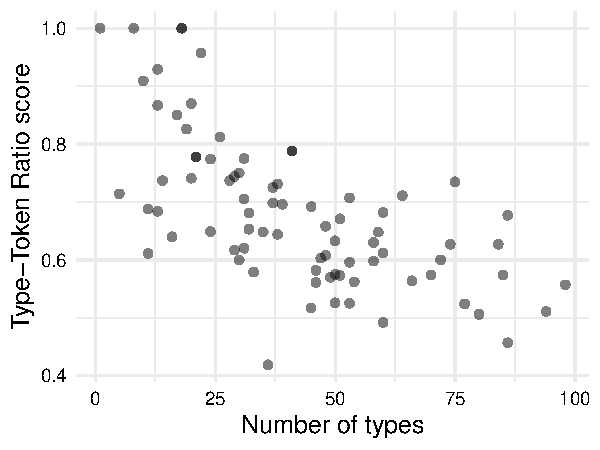
\includegraphics{part_2/3_analysis_files/figure-pdf/fig-analysis-belc-scatter-plot-1.pdf}

}

\subcaption{\label{fig-analysis-belc-scatter-plot-1}Points}

\end{minipage}%
%
\begin{minipage}{0.50\linewidth}

\centering{

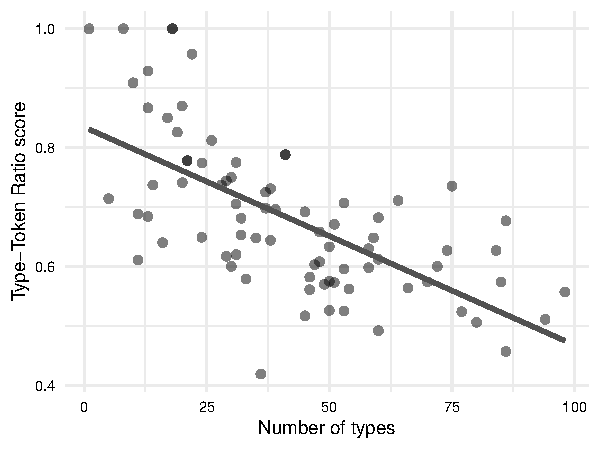
\includegraphics{part_2/3_analysis_files/figure-pdf/fig-analysis-belc-scatter-plot-2.pdf}

}

\subcaption{\label{fig-analysis-belc-scatter-plot-2}Points with a linear
trend line}

\end{minipage}%

\caption{\label{fig-analysis-belc-scatter-plot}Scatter plot for the
relationship between \texttt{ttr} and \texttt{types} in the BELC
dataset}

\end{figure}%

\section{Analyze}\label{sec-analysis-analyze}

The goal of analysis, generally, is to generate knowledge from
information. The type of knowledge generated and the process by which it
is generated, however, differ and can be broadly grouped into three
analysis types: exploratory, predictive, and inferential.

In this section, I will elaborate briefly on the distinctions between
analysis types seen in Table~\ref{tbl-analysis-analysis-types}. I will
structure the discussion moving from the least structured (inductive) to
most structured (deductive) approach to deriving knowledge from
information with the aim to provide enough information for you to
identify these research approaches in the literature and to make
appropriate decisions as to which approach your research should adopt.

\begin{longtable}[]{@{}
  >{\raggedright\arraybackslash}p{(\columnwidth - 8\tabcolsep) * \real{0.1500}}
  >{\raggedright\arraybackslash}p{(\columnwidth - 8\tabcolsep) * \real{0.1900}}
  >{\raggedright\arraybackslash}p{(\columnwidth - 8\tabcolsep) * \real{0.2200}}
  >{\raggedright\arraybackslash}p{(\columnwidth - 8\tabcolsep) * \real{0.2200}}
  >{\raggedright\arraybackslash}p{(\columnwidth - 8\tabcolsep) * \real{0.2200}}@{}}
\caption{Overview of analysis
types}\label{tbl-analysis-analysis-types}\tabularnewline
\toprule\noalign{}
\begin{minipage}[b]{\linewidth}\raggedright
Type
\end{minipage} & \begin{minipage}[b]{\linewidth}\raggedright
Aims
\end{minipage} & \begin{minipage}[b]{\linewidth}\raggedright
Approach
\end{minipage} & \begin{minipage}[b]{\linewidth}\raggedright
Methods
\end{minipage} & \begin{minipage}[b]{\linewidth}\raggedright
Evaluation
\end{minipage} \\
\midrule\noalign{}
\endfirsthead
\toprule\noalign{}
\begin{minipage}[b]{\linewidth}\raggedright
Type
\end{minipage} & \begin{minipage}[b]{\linewidth}\raggedright
Aims
\end{minipage} & \begin{minipage}[b]{\linewidth}\raggedright
Approach
\end{minipage} & \begin{minipage}[b]{\linewidth}\raggedright
Methods
\end{minipage} & \begin{minipage}[b]{\linewidth}\raggedright
Evaluation
\end{minipage} \\
\midrule\noalign{}
\endhead
\bottomrule\noalign{}
\endlastfoot
Exploratory & Explore: gain insight & Inductive, data-driven, and
iterative & Descriptive, pattern detection with machine learning
(unsupervised) & Associative \\
Predictive & Predict: validate associations & Semi-deductive, data-/
theory-driven, and iterative & Predictive modeling with machine learning
(supervised) & Model performance, feature importance, and associative \\
Inferential & Explain: test hypotheses & Deductive, theory-driven, and
non-iterative & Hypothesis testing with statistical tests & Causal \\
\end{longtable}

\subsection{Explore}\label{sec-analysis-explore}

In \textbf{Exploratory Data Analysis (EDA)}, we use a variety of methods
to identify patterns, trends, and relations within and between
variables. The goal of EDA is uncover insights in an inductive,
data-driven manner. That is to say, that we do not enter into EDA with a
fixed hypothesis in mind, but rather we explore intuition, probe
anecdote, and follow hunches to identify patterns and relationships and
to evaluate whether and why they are meaningful. We are admittedly
treading new or unfamiliar terrain letting the data guide our analysis.
This means that we can use and reuse the same data to explore different
angles and approaches adjusting our methods and measures as we go. In
this way, EDA is an iterative, meaning generating process.

In line with the investigative nature of EDA, the identification of
variables of interest is a discovery process. We most likely have a
intuition about the variables we would like to explore, but we are able
to adjust our variables as need be to suit our research aims. When the
identification and selection of variables is open, the process is known
as \textbf{feature engineering}. A process that is much an art as a
science, feature engineering leverages a mixture of relevant domain
knowledge, intuition, and trial and error to identify features that
serve to best represent the data and to best serve the research aims.
Furthermore, the roles of features in EDA are fluid --no variable has a
special status, as seen in Figure~\ref{fig-eda-variables}. We will see
that in other types of analysis, some or all the roles of the variables
are fixed.

\begin{figure}[!htb]

\centering{

{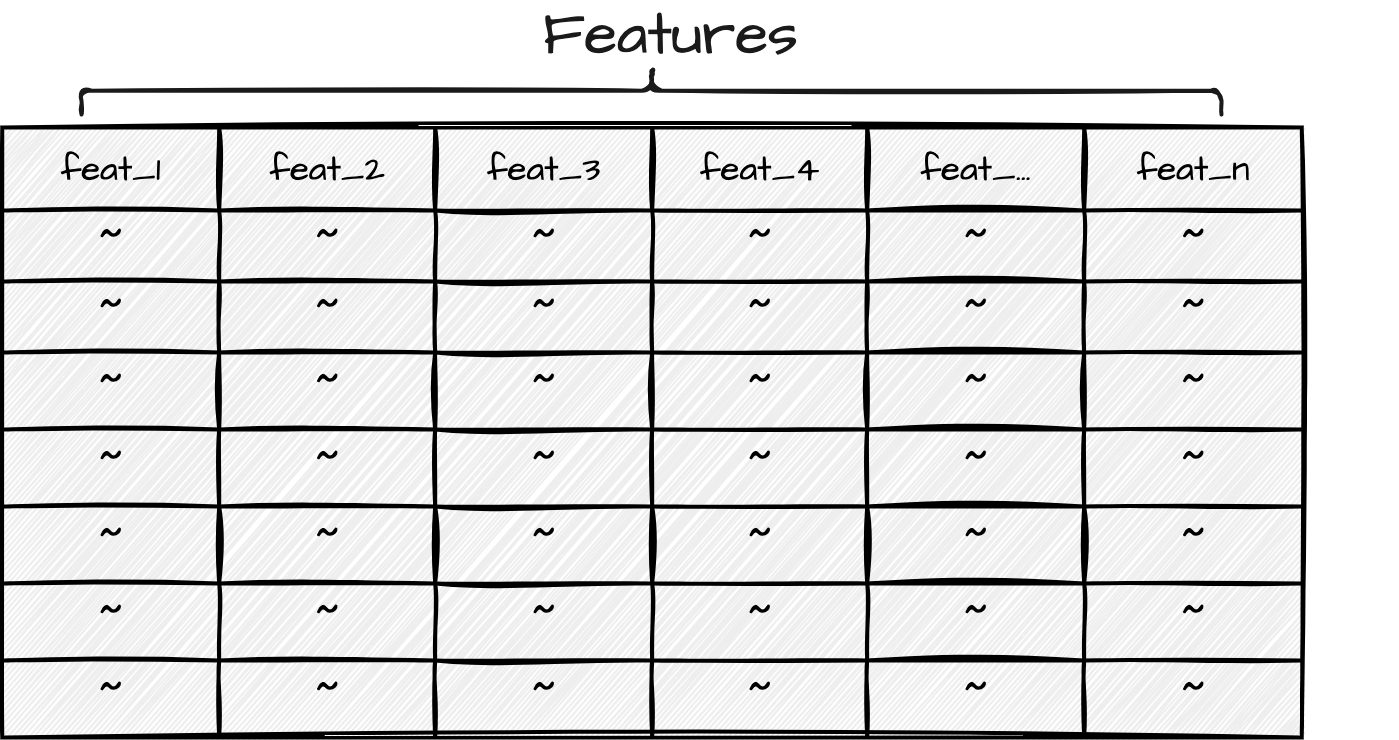
\includegraphics{part_2/figures/analysis-eda-variables.drawio.png}}

}

\caption{\label{fig-eda-variables}Roles of variables in exploratory data
analysis}

\end{figure}%

Any given dataset could serve as a starting point to explore many
different types of research questions. In order to maintain research
coherence so our efforts to not careen into a free-for-all, we need to
tether our feature engineering to a unit of analysis that is relevant to
the research question. A \textbf{unit of analysis} is the entity that we
are interested in studying. Not to be confused with the unit of
observation, which is the entity that we are able to observe and measure
(\citeproc{ref-Sedgwick2015}{Sedgwick, 2015}). Depending on the
perspective we are interested in investigating, the choice of how to
approach engineering features to gain insight will vary.

By the same token, approaches for interrogating the dataset can differ
significantly, between research projects and within the same project,
but for instructive purposes, let's draw a distinction between
descriptive methods and unsupervised learning methods, as seen in
Table~\ref{tbl-eda-methods}.

\begin{longtable}[]{@{}
  >{\raggedright\arraybackslash}p{(\columnwidth - 2\tabcolsep) * \real{0.5000}}
  >{\raggedright\arraybackslash}p{(\columnwidth - 2\tabcolsep) * \real{0.5000}}@{}}
\caption{Some common exploratory data analysis
methods}\label{tbl-eda-methods}\tabularnewline
\toprule\noalign{}
\begin{minipage}[b]{\linewidth}\raggedright
Descriptive methods
\end{minipage} & \begin{minipage}[b]{\linewidth}\raggedright
Unsupervised learning methods
\end{minipage} \\
\midrule\noalign{}
\endfirsthead
\toprule\noalign{}
\begin{minipage}[b]{\linewidth}\raggedright
Descriptive methods
\end{minipage} & \begin{minipage}[b]{\linewidth}\raggedright
Unsupervised learning methods
\end{minipage} \\
\midrule\noalign{}
\endhead
\bottomrule\noalign{}
\endlastfoot
Frequency analysis & Cluster analysis \\
Co-occurence analysis & Principal component analysis \\
Keyness analysis & Topic Modeling \\
& Vector space models \\
\end{longtable}

The first group, \textbf{descriptive methods} can be seen as an
extenstion of the descriptive statistics covered earlier in this chapter
including statistic, tabular, and visual techniques. The second group,
\textbf{unsupervised learning}, is a subtype of machine learning in
which an algorithm is used to find patterns within and between variables
in the data without any guidance (supervision). In this way, the
algorithm, or machine learner, is left to make connections and
associations wherever they may appear in the input data.

Either through descriptive, unsupervised learning methods, or a
combination of both, EDA employs quantitative methods to summarize,
reduce, and sort complex datasets in order to provide the researcher
novel perspective to be qualitatively assessed. Exploratory methods
produce results that require associative thinking and pattern detection.
Speculative as they are, the results from exploratory methods can be
highly informative and lead to new insight and inspire further study in
directions that may not have been expected.

\subsection{Predict}\label{sec-analysis-predict}

\textbf{Predictive Data Analysis (PDA)} employs a variety of techniques
to examine and evaluate the association strength between a variable or
set of variables, with a specific focus on predicting a target variable.
The aim of PDA is to construct models that can accurately forecast
future outcomes, using either data-driven or theory-driven approaches.
In this process, \textbf{supervised learning} methods, where the machine
learning algorithm is guided (supervised) by a target outcome variable,
are used. This means we don't begin PDA with a completely open-ended
exploration, but rather with an objective - accurate predictions.
However, the path to achieving this objective can be flexible, allowing
us freedom to adjust our models and methods. Unlike EDA, where the
entire dataset can be reused for different approaches, PDA requires a
portion of the data to be reserved for evaluation, enhancing the
validity of our predictive models. Thus, PDA is an iterative process
that combines the flexibility of exploratory analysis with the rigor of
confirmatory analysis.

There are two types of variables in PDA: the outcome variable and the
predictor variables, or features. The \textbf{outcome variable} is the
variable that the researcher is trying to predict. It is the only
variable that is necessarily fixed as part of the research question. The
features are the variables that are used to predict the outcome
variable. An overview of the roles of these variables in PDA is shown in
Figure~\ref{fig-pda-variables}.

\begin{figure}[!htb]

\centering{

{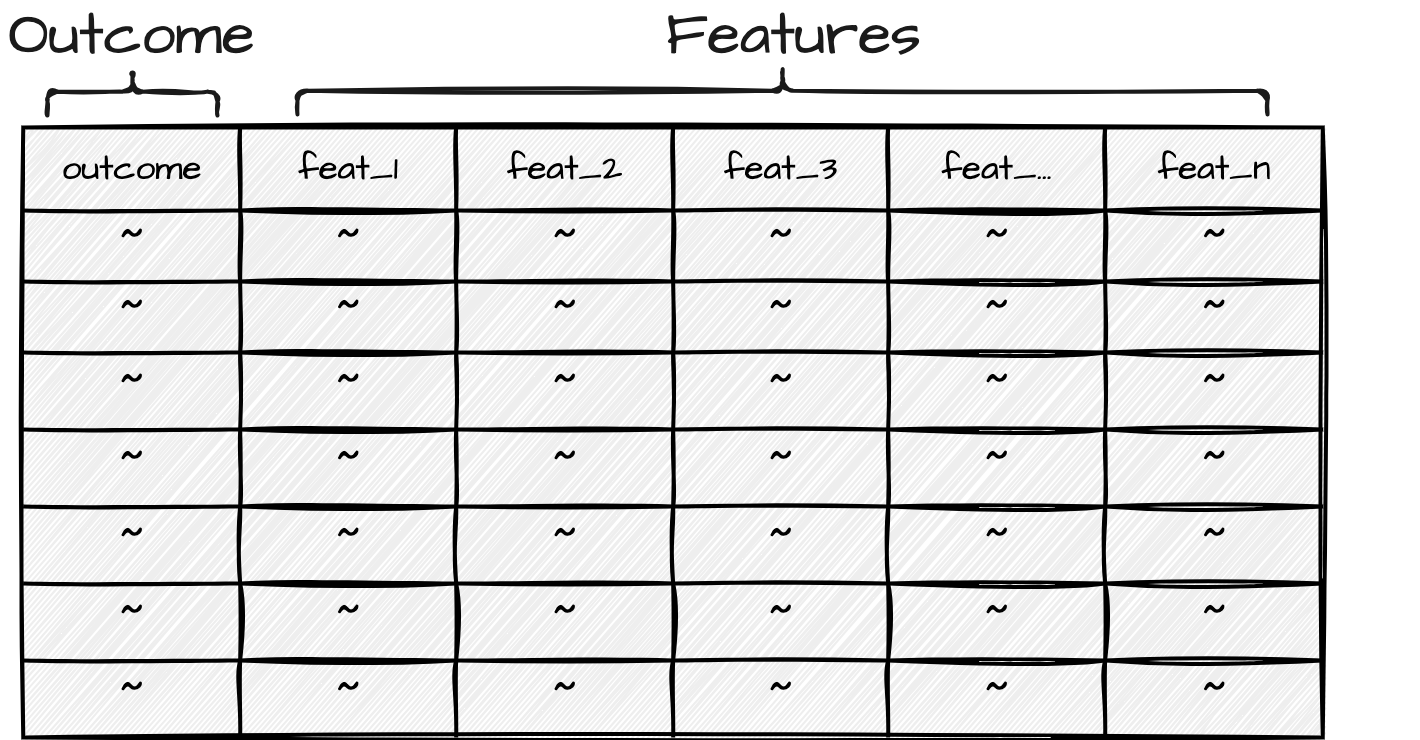
\includegraphics{part_2/figures/analysis-pda-variables.drawio.png}}

}

\caption{\label{fig-pda-variables}Roles of variables in predictive data
analysis}

\end{figure}%

Feature selection can be either data-driven or theory-driven.
Data-driven features are those that are engineered to enhance predictive
power, while theory-driven features are those that are selected based on
theoretical relevance.

The approach to interrogating the dataset includes three main steps:
feature engineering, model selection, and model evaluation. We've
discussed feature engineering, so what is model selection and model
evaluation?

\textbf{Model selection} is the process of choosing a machine learning
algorithm and set of features that produces the best prediction accuracy
for the outcome variable. To refine our approach such that we arrive at
the best combination of algorithm and features, we need to train our
machine learner on a variety of combinations and evaluate the accuracy
of each.

There are many different types of machine learning algorithms, each with
their own strengths and weaknesses. The first rough cut is to decide
what type of outcome variable we are predicting: categorical or numeric.
If the outcome variable is categorical, we are performing a
\textbf{classification} task, and if the outcome variable is numeric, we
are performing a \textbf{regression} task. As we see in
Table~\ref{tbl-pda-algorithms}, there are various algorithms that can be
used for each task.

\begin{longtable}[]{@{}
  >{\raggedright\arraybackslash}p{(\columnwidth - 2\tabcolsep) * \real{0.5000}}
  >{\raggedright\arraybackslash}p{(\columnwidth - 2\tabcolsep) * \real{0.5000}}@{}}
\caption{Some common supervised learning algorithms used in
PDA}\label{tbl-pda-algorithms}\tabularnewline
\toprule\noalign{}
\begin{minipage}[b]{\linewidth}\raggedright
Classification
\end{minipage} & \begin{minipage}[b]{\linewidth}\raggedright
Regression
\end{minipage} \\
\midrule\noalign{}
\endfirsthead
\toprule\noalign{}
\begin{minipage}[b]{\linewidth}\raggedright
Classification
\end{minipage} & \begin{minipage}[b]{\linewidth}\raggedright
Regression
\end{minipage} \\
\midrule\noalign{}
\endhead
\bottomrule\noalign{}
\endlastfoot
Logistic Regression & Linear Regression \\
Random Forest Classifier & Random Forest Regressor \\
Support Vector Machine & Support Vector Regression \\
Neural Network Classifier & Neural Network Regressor \\
\end{longtable}

There are a number of algorithm-specific strengths and weaknesses to be
considered in the process of model selection. These hinge on
characteristics of the data, such as the size of the dataset, the number
of features, the type of features, and the expected type of
relationships between features or on computing resources, such as the
amount of time available to train the model or the amount of memory
available to store the model.

\textbf{Model evaluation} is the process of assessing the accuracy of
the model on the test set, which is a proxy for how well the model will
generalize to new data. Model evaluation is performed quantitatively by
calculating the accuracy of the model. It is important to note that
whether the accuracy metrics are good is to some degree qualitative
judgment.

\subsection{Infer}\label{sec-analysis-infer}

The most commonly recognized of the three data analysis approaches,
\textbf{Inferential data analysis (IDA)} is the bread-and-butter of
science. IDA is a deductive, theory-driven approach in which all aspects
of analysis stem from a pre-determined premise, or hypothesis, about the
nature of a relationship in the world and then aims to test whether this
relationship is statistically supported given the evidence. Since the
goal is to infer conclusions about a certain relationship in the
population based on a statistical evaluation of a (corpus) sample, the
representativeness of the sample is of utmost importance. Furthermore,
the use of the data is limited to the scope of the hypothesis --that is,
the data cannot be used iteratively for exploratory purposes.

The selection of variables and the roles they play in the analysis are
determined by the hypothesis. In a nutshell, a \textbf{hypothesis} is a
formal statement about the state of the world. This statement is
theory-driven meaning that it is predicated on previous research. We are
not exploring or examining relationships, rather we are testing a
specific relationship. In practice, however, we are in fact proposing
two mutally exclusive hypotheses. The first is the \textbf{Alternative
Hypothesis}, or \(H_1\). This is the hypothesis I just described --the
statement grounded in the previous literature outlining a predicted
relationship. The second is the \textbf{Null Hypothesis}, or \(H_0\).
This is the flip-side of the hypothesis testing coin and states that
there is no difference or relationship. Together \(H_1\) and \(H_0\)
cover all logical outcomes.

Now, in standard IDA one variable is the response variable and one or
more variables are explanatory variables. The \textbf{response
variable}, sometimes referred to as the outcome or dependent variable,
is the variable which contains the information which is hypothesized to
depend on the information in the explanatory variable(s). It is the
variable whose variation a research study seeks to explain. An
\textbf{explanatory variable}, sometimes referred to as a independent or
predictor variable, is a variable whose variation is hypothesized to
explain the variation in the response variable.

Explanatory variables add to the complexity of a study because they are
part of our research focus, specifically our hypothesis. It is, however,
common to include other variables which are not of central focus, but
are commonly assumed to contribute to the explanation of the variation
of the response variable. These are known as \textbf{control variables}.
Control variables are included in the analysis to account for the
influence of other variables on the relationship between the response
and explanatory variables, but will not be included in the hypothesis
nor interpreted in our results.

We can now see in Figure~\ref{fig-analysis-ida-variables} the variables
roles assigned to variables in a hypothesis-driven study.

\begin{figure}[!htb]

\centering{

{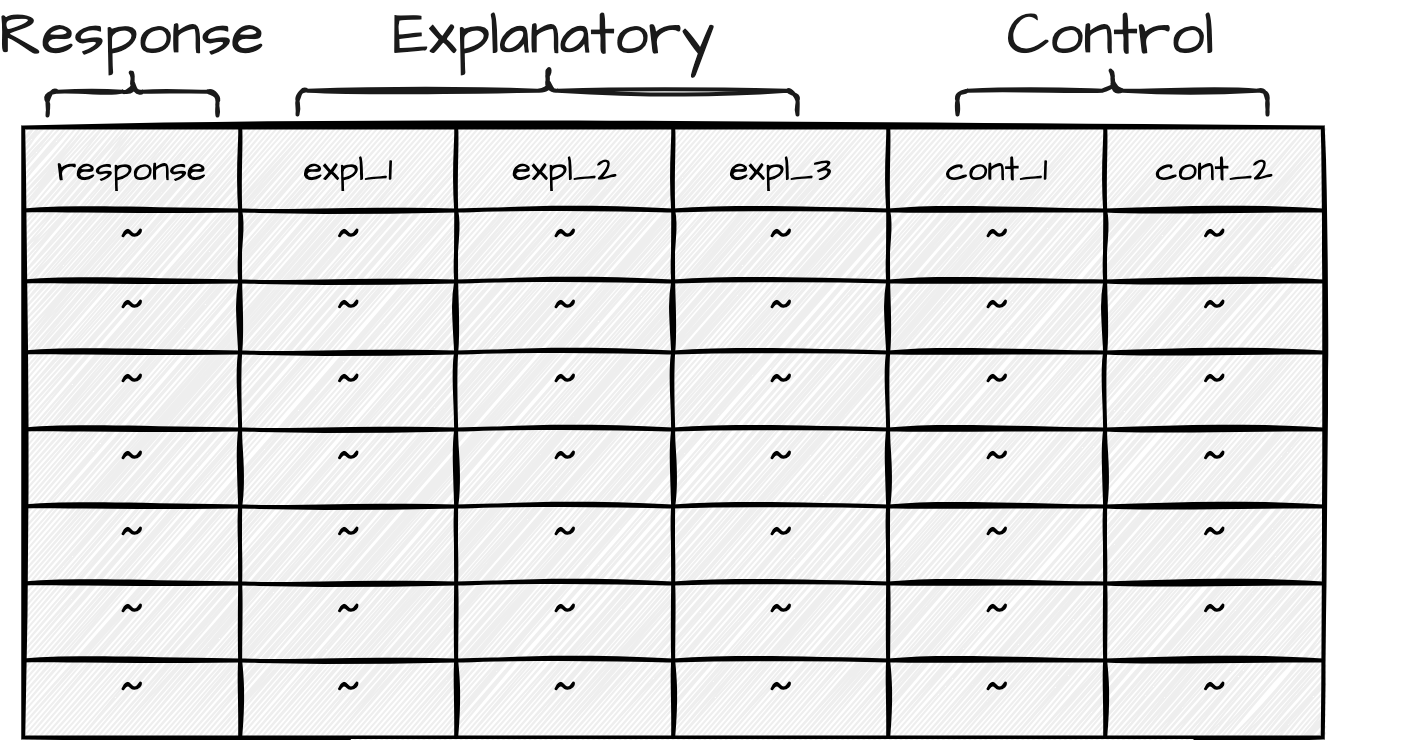
\includegraphics{part_2/figures/analysis-ida-variables.drawio.png}}

}

\caption{\label{fig-analysis-ida-variables}Roles of variables in
inferential data analysis}

\end{figure}%

The type of statistical test that one chooses is based on (1) the
informational value of the dependent variable and (2) the number of
predictor variables included in the analysis. Together these two
characteristics go a long way in determining the appropriate class of
statistical test (see S. Th. Gries (\citeproc{ref-Gries2013a}{2013}) and
Paquot \& Gries (\citeproc{ref-Paquot2020a}{2020}) for a more exhaustive
description).

IDA relies heavily on quantitative evaluation methods to draw
conclusions that can be generalized to the target population. It is key
to understand that our goal in hypothesis testing is not to find
evidence in support of \(H_1\), but rather to assess the likelihood that
we can reliably reject \(H_0\).

Traditionally, \(p\)-values have been used to determine the likelihood
of rejecting \(H_0\). A \(p\)-value is the probability of observing a
test statistic as extreme as the one observed, given that \(H_0\) is
true. However, \(p\)-values are not the only metric used to evaluate the
likelihood of rejecting \(H_0\). Other metrics, such as effect size and
confidence intervals, are also used to interpret the results of
hypothesis tests.

\section{Communicate}\label{sec-analysis-communicate}

Conducting research should be enjoyable and personally rewarding but the
effort you have invested and knowledge you have generated should be
shared with others. Whether part of a blog, presentation, journal
article, or for your own purposes it is important to document your
analysis results and process in a way that is informative and
interpretable. This enhances the value of your work, allowing others to
learn from your experience and build on your findings.

\subsection{Report}\label{sec-analysis-report}

The most widely recognized form of communicating research is through a
report. A report is a narrative of your analysis, including the research
question, the data you used, the methods you applied, and the results
you obtained. We are both reporting our findings and documenting our
process to inform others of what we did and why we did it but also to
invite readers to evaluate our findings for themselves. The scientific
process is a collaborative one and evaluation by peers is a key
component of the process.

\subsection{Document}\label{sec-analysis-document}

While a good report will include the most vital information to
understand the procedures, results, and findings of an analysis, there
is much more information generated in the course of an analysis which
does not traditionally appear in prose. If a research project is
conducted programmatically, however, data, code, and documentation can
be made available to others as part of the communication process.
Increasingly, researchers are sharing their data and code as part of the
publication process. This allows others to reproduce the analysis and
verify the results contributing to the collaborative nature of the
scientific process.

Together, data, code, and documentation form a \textbf{research
compendium}. As you can imagine the research process can quickly become
complex and unwieldy as the number of files and folders grows. If not
organized properly, it can be difficult to find the information you
need. Furthermore, if not documented, decisions made in the course of
the analysis can be difficult or impossible to trace. For this reason,
it is recommendable to follow a set of best practices for organizing and
documenting your research compendium. We will cover this in more detail
in subsequent chapters.

\section*{Activities}\label{activities-1}
\addcontentsline{toc}{section}{Activities}

\markright{Activities}

In the following activies, we will build on our understanding of how to
summarize data using statistics, tables, and plots. We will dive deeper
into the use of \{skimr\} (\citeproc{ref-R-skimr}{Waring et al., 2022})
to summarize data and the \texttt{ggplot2} package
(\citeproc{ref-R-ggplot2}{Wickham, Chang, et al., 2024}) to create
plots. We also introduce producing Quarto tables and figures with
appropriate code block options. We will reinforce our understanding of
\{readr\} (\citeproc{ref-R-readr}{Wickham, Hester, \& Bryan, 2024}) to
read in data and \{dplyr\} (\citeproc{ref-R-dplyr}{Wickham, François,
Henry, Müller, \& Vaughan, 2023}) to manipulate data.

\begin{tcolorbox}[enhanced jigsaw, left=2mm, toprule=.15mm, colback=white, colframe=quarto-callout-color-frame, arc=.35mm, rightrule=.15mm, bottomrule=.15mm, leftrule=.75mm, breakable, opacityback=0]

\textbf{\faIcon{file-code} Recipe}

\textbf{What}: Descriptive assessment of datasets\\
\textbf{How}: Read Recipe 3, complete comprehension check, and prepare
for Lab 3.\\
\textbf{Why}: To explore appropriate methods for summarizing variables
in datasets given the number and informational values of the
variable(s).

\end{tcolorbox}

\begin{tcolorbox}[enhanced jigsaw, left=2mm, toprule=.15mm, colback=white, colframe=quarto-callout-color-frame, arc=.35mm, rightrule=.15mm, bottomrule=.15mm, leftrule=.75mm, breakable, opacityback=0]

\textbf{\faIcon{flask} Lab}

\textbf{What}: Trace the datascape\\
\textbf{How}: Clone, fork, and complete the steps in Lab 3.\\
\textbf{Why}: To identify and apply the appropriate descriptive methods
for a vector's informational value and to assess both single variables
and multiple variables with the appropriate statistical, tabular, and/
or graphical summaries.

\end{tcolorbox}

\section*{Summary}\label{summary-2}
\addcontentsline{toc}{section}{Summary}

\markright{Summary}

In this chapter we have focused on description and analysis --the third
component of DIKI Hierarchy. This is the stage where we begin to derive
knowledge from the data which includes first performing a descriptive
assessment of the individual variables and relationships between
variables. Only after we have a better understanding of our data, we
move to the analysis stage. We outlined three data analysis types in
this chapter: exploratory, predictive, and inferential. Each of these
embodies distinct approaches to deriving knowledge from data. Ultimately
the choice of analysis type is highly dependent on the goals of the
research.

I rounded out this chapter with a short description of the importance of
communicating the analysis process and results. Reporting, in its
traditional form, is documented in prose in an article. Yet even the
most detailed reporting in a write-up still leaves many practical, but
key, points of the analysis obscured. A programming approach provides
the procedural steps taken that when shared provide the exact methods
applied. Together with the write-up, a research compendium which
provides the scripts to run the analysis and documentation on how to run
the analysis forms an integral part of creating reproducible research.

\chapter{Research}\label{sec-research-chapter}

\begin{quote}
Thus, the task is, not so much to see what no one has seen yet; but to
think what nobody has thought yet, about that what everybody sees.

--- Erwin Schrödinger
\end{quote}

\begin{tcolorbox}[enhanced jigsaw, left=2mm, toprule=.15mm, colback=white, colframe=quarto-callout-color-frame, arc=.35mm, rightrule=.15mm, bottomrule=.15mm, leftrule=.75mm, breakable, opacityback=0]

\textbf{\faIcon{list-alt} Outcomes}

\begin{itemize}
\tightlist
\item
  Identify a research area and problem by listing key strategies and
  describing their contribution towards research identification.
\item
  Explain the significance of a well-framed research question in guiding
  the overall research project.
\item
  Comprehend how the conceptual and practical steps involved in
  developing a research blueprint aid not only the researcher but also
  the broader scientific community.
\end{itemize}

\end{tcolorbox}

In this chapter, we discuss how to frame research, that is how to
position your research project's findings to contribute insight to
understanding of the world. We will cover how to connect with the
literature, selecting a research area and identifying a research
problem, and how to design research best positioned to return relevant
findings that will connect with this literature, establishing a research
aim and research question. We will round out this chapter with a guide
on developing a research blueprint --a working plan to organize the
conceptual and practical steps to implement the research effectively and
in a way that supports communicating the research findings and the
process by which the findings were obtained.

\begin{tcolorbox}[enhanced jigsaw, left=2mm, toprule=.15mm, colback=white, colframe=quarto-callout-color-frame, arc=.35mm, rightrule=.15mm, bottomrule=.15mm, leftrule=.75mm, breakable, opacityback=0]

\textbf{\faIcon{terminal} Lessons}

\textbf{What}: Project Environment\\
\textbf{How}: In an R console, load \{swirl\}, run \texttt{swirl()}, and
follow prompts to select the lesson.\\
\textbf{Why}: To highlight the importance of the computing environment
in R for project management and reproducibility.

\end{tcolorbox}

\section{Frame}\label{sec-research-frame}

Together a research area, problem, aim and question and the research
blueprint that forms the conceptual and practical scaffolding of the
project ensure from the outset that the project is solidly grounded in
the main characteristics of good research. These characteristics,
summarized by Cross (\citeproc{ref-Cross2006}{2006}), are found in
Table~\ref{tbl-research-cross-research-char-table}.

\begin{longtable}[]{@{}
  >{\raggedright\arraybackslash}p{(\columnwidth - 2\tabcolsep) * \real{0.2000}}
  >{\raggedright\arraybackslash}p{(\columnwidth - 2\tabcolsep) * \real{0.8000}}@{}}
\caption{Characteristics of good research (Cross,
2006)}\label{tbl-research-cross-research-char-table}\tabularnewline
\toprule\noalign{}
\begin{minipage}[b]{\linewidth}\raggedright
Characteristic
\end{minipage} & \begin{minipage}[b]{\linewidth}\raggedright
Description
\end{minipage} \\
\midrule\noalign{}
\endfirsthead
\toprule\noalign{}
\begin{minipage}[b]{\linewidth}\raggedright
Characteristic
\end{minipage} & \begin{minipage}[b]{\linewidth}\raggedright
Description
\end{minipage} \\
\midrule\noalign{}
\endhead
\bottomrule\noalign{}
\endlastfoot
Purposive & Based on identification of an issue or problem worthy and
capable of investigation \\
Inquisitive & Seeking to acquire new knowledge \\
Informed & Conducted from an awareness of previous, related research \\
Methodical & Planned and carried out in a disciplined manner \\
Communicable & Generating and reporting results which are feasible and
accessible by others \\
\end{longtable}

With these characteristics in mind, let's get started with the first
component to address --connecting with the literature.

\section{Connect}\label{sec-research-connect}

\subsection{Research area}\label{research-area}

The first decision to make in the research process is to identify a
research area. A \textbf{research area} is a general area of interest
where a researcher wants to derive insight and make a contribution to
understanding. For those with an established research trajectory in
language, the area of research to address through text analysis will
likely be an extension of their prior work. For others, which include
new researchers or researchers that want to explore new areas of
language research or approach an area through a language-based lens, the
choice of area may be less obvious. In either case, the choice of a
research area should be guided by a desire to contribute something
relevant to a theoretical, applied, and/ or practical matter of personal
interest. Personal relevance goes a long way to developing and carrying
out \emph{purposive} and \emph{inquisitive} research.

So how do we get started? Consider your interests in a language or set
of languages, a discipline, a methodology, or some applied area.
Language is at the heart of the human experience and therefore found in
some fashion anywhere one seeks to find it. But it is a big world and
more often than not the general question about what area to explore
language use is sometimes the most difficult. To get the ball rolling,
it is helpful to peruse disciplinary encyclopedias or handbooks of
linguistics and language-related an academic fields (\emph{e.g.}
Encyclopedia of Language and Linguistics
(\citeproc{ref-Brown2005}{Brown, 2005}), A Practical Guide to Electronic
Resources in the Humanities (\citeproc{ref-Dubnjakovic2010}{Dubnjakovic
\& Tomlin, 2010}), Routledge encyclopedia of translation technology
(\citeproc{ref-Chan2014}{Chan, 2014}))

A more personal, less academic, approach is to consult online forums,
blogs, \emph{etc}. that one already frequents or can be accessed via an
online search. Through social media you may find particular people that
maintain a blog worth browsing. Perusing these resources can help spark
ideas and highlight the kinds of questions that interest you.

Regardless of whether your inquiry stems from academic, professional, or
personal interest, try to connect these findings to academic areas of
research. Academic research is highly structured and well-documented and
making associations with this network will aid in subsequent steps in
developing a research project.

\subsection{Research problem}\label{sec-research-problem}

Once you've made a rough-cut decision about the area of research, it is
now time to take a deeper dive into the subject area and jump into the
literature. This is where the rich structure of disciplinary research
will provide aid to traverse the vast world of academic knowledge and
identify a research problem. A \textbf{research problem} highlights a
particular topic of debate or uncertainty in existing knowledge which is
worthy of study.

Surveying the relevant literature is key to ensuring that your research
is \emph{informed}, that is, connected to previous work. Identifying
relevant research to consult can be a bit of a `chicken or the egg'
problem --some knowledge of the area is necessary to find relevant
topics, some knowledge of the topics is necessary to narrow the area of
research. Many times the only way forward is to jump into conducting
searches. These can be world-accessible resources (\emph{e.g.} Google
Scholar) or limited-access resources that are provided through an
academic institution (\emph{e.g.} Linguistics and Language Behavior
Abstracts, ERIC, PsycINFO, \emph{etc.}). Some organizations and academic
institutions provide research guides to help researcher's access the
primary literature. There are even a new breed of search engines that
are designed to help researchers aggregate and search academic
literature (\emph{e.g.} Scite, Elicit, \emph{etc.}). Another avenue to
explore are journals and conference proceedings dedicated to linguistics
and language-related research. Text analysis is a rapidly expanding
methodology which is being applied to a wide range of research areas.

To explore research related to text analysis it is helpful to start with
the (sub)discipline name(s) you identified in when selecting your
research area, more specific terms that occur to you or key terms from
the literature, and terms such as `corpus study' or `corpus-based'. The
results from first searches may not turn out to be sources that end up
figuring explicitly in your research, but it is important to skim these
results and the publications themselves to mine information that can be
useful to formulate better and more targeted searches.

Relevant information for honing your searches can be found throughout an
academic publication. However, pay particular attention to the abstract,
in articles, and the table of contents, in books, and the cited
references. Abstracts and tables of contents often include
discipline-specific jargon that is commonly used in the field. In some
articles, there is even a short list of key terms listed below the
abstract which can be extremely useful to seed better and more precise
search results. The references section will contain relevant and
influential research. Scan these references for publications which
appear to narrowing in on topic of interest and treat it like a search
in its own right.

Once your searches begin to show promising results it is time to keep
track and organize these references. Whether you plan to collect
thousands of references over a lifetime of academic research or your aim
is centered around one project, software such as
\href{https://www.zotero.org/}{Zotero}\footnote{\href{https://guides.zsr.wfu.edu/zotero}{Zotero
  Guide}},
\href{https://www.mendeley.com/reference-management/reference-manager}{Mendeley},
or \href{https://bibdesk.sourceforge.io/}{BibDesk} provide powerful,
flexible, and easy-to-use tools to collect, organize, annotate, search,
and export references. Citation management software is indispensable for
modern research --and often free!

As your list of relevant references grows, you will want to start the
investigation process in earnest. Begin skimming (not reading) the
contents of each of these publications, starting with what appears to be
the most relevant first. Annotate these publications using highlighting
features of the citation management software to identify: (1) the stated
goal(s) of the research, (2) the data source(s) used, (3) the
information drawn from the data source(s), (4) the analysis approach
employed, and (5) the main finding(s) of the research as they pertain to
the stated goal(s).

Next, in your own words, summarize these five key areas in prose adding
your summary to the notes feature of the citation management software.
This process will allow you to efficiently gather and document
references with the relevant information to guide the identification of
a research problem, to guide the formation of your problem statement,
and ultimately, to support the literature review that will figure in
your project write-up.

From your preliminary annotated summaries you will undoubtedly start to
recognize overlapping and contrasting aspects in the research
literature. These aspects may be topical, theoretical, methodological,
or appear along other lines. Note these aspects and continue to conduct
more refine searches, annotate new references, and monitor for any
emerging uncertainties, limitations, debates, and/ or contraditions
which align with your research interest(s). When a promising pattern
takes shape, it is time to engage with a more detailed reading of those
references which appear most relevant highlighting the potential gap(s)
in the literature.

At this point you can focus energy on more nuanced aspects of a
particular gap in the literature with the goal to formulate a problem
statement. A \textbf{problem statement} directly acknowledges a gap in
the literature and puts a finer point on the nature and relevance of
this gap for understanding. This statement reflects your first
deliberate attempt to establish a line of inquiry. It will be a
targeted, but still somewhat general, statement framing the gap in the
literature that will guide subsequent research design decisions.

\section{Define}\label{sec-research-define}

\subsection{Research aim}\label{sec-research-aim}

With a problem statement in hand, it is now time to consider the goal(s)
of the research. A \textbf{research aim} frames the type of inquiry to
be conducted. Will the research aim to explore, predict, or explain? As
you can appreciate, the research aim is directly related to the analysis
methods we touched upon in \hyperref[sec-approaching-analysis]{Chapter
3}.

To gauge how to frame your research aim, reflect on the literature that
led you to your problem statement and the nature of the problem
statement itself. If the gap at the center of the problem statement is a
lack of knowledge, your research aim may be exploratory. If the gap
concerns a conjecture about a relationship, then your research may take
a predictive approach. When the gap points to the validation of a
relationship, then your research will likely be inferential in nature.
Before selecting your research aim it is also helpful to consult the
research aims of the primary literature that led you to your research
statement.

Typically, a problem statement addressing a subtle, specific issue tends
to adopt research objectives similar to prior studies. In contrast, a
statement focusing on a broader, more distinct issue is likely to have
unique research goals. Yet, this is more of a guideline than a strict
rule.

It's crucial to understand both the existing literature and the nature
of various types of analyses. Being clear about your research goals is
important to ensure that your study is well-placed to produce results
that add value to the current understanding in an informed manner.

\subsection{Research question}\label{sec-research-question}

The next step in research design is to craft the research question. A
\index{research question}\textbf{research question} is clearly defined
statement which identifies an aspect of uncertainty and the particular
relationships that this uncertainty concerns. The research question
extends and narrows the line of inquiry established in the research
statement and research aim. To craft a research question, we can use the
research statment for the content and the research aim for the form.

\subsubsection{Form}\label{sec-research-question-form}

The form of a research question will vary based on the research aim,
which as I mentioned, is inimately connected to the analysis approach.
For inferential-based research, the research question will actually be a
statement, not a question. This statement makes a testable claim about
the nature of a particular relationship --\emph{i.e.} asserts a
hypothesis.

For illustration, let's posit a hypothesis (\(H_1\)), leaving aside the
implicit null hypothesis (\(H_0\)), seen in
Example~\ref{exm-research-form-infer}.

\begin{example}[]\protect\hypertarget{exm-research-form-infer}{}\label{exm-research-form-infer}

\emph{Women use more questions than men in spontaneous conversations.}

\end{example}

For predictive- and exploratory-based research, the research question is
in fact a question. A reframing of the example hypothesis for a
predictive-based research question might take the form seen in
Example~\ref{exm-research-form-pred}.

\begin{example}[]\protect\hypertarget{exm-research-form-pred}{}\label{exm-research-form-pred}

\emph{Can the number of questions used in spontaneous conversations
predict if a speaker is male or female?}

\end{example}

And a similar exploratory-based research question might take the form
seen in Example~\ref{exm-research-form-exp}.

\begin{example}[]\protect\hypertarget{exm-research-form-exp}{}\label{exm-research-form-exp}

\emph{Do men and women differ in terms of the number of questions they
use in spontaneous conversations?}

\end{example}

The central research interest behind these hypothetical research
questions is, admittedly, quite basic. But from these simplified
examples, we are able to appreciate the similarities and differences
between the forms of research statements that correspond to distinct
research aims.

\subsubsection{Content}\label{sec-research-question-content}

In terms of content, the research question will make reference to two
key components. First, is the unit of analysis. The \textbf{unit of
analysis} is the entity which the research aims to investigate. For our
three example research aims, the unit of analysis is the same, namely
\emph{speakers}. Note, however, that the current unit of analysis is
somewhat vague in the example research questions. A more precise unit of
analysis would include more information about the population from which
the speakers are drawn (\emph{i.e.} English speakers, American English
speakers, American English speakers of the Southeast, \emph{etc}.).

The second key component is the unit of observation. The \textbf{unit of
observation} is the primary element on which the insight into the unit
of analysis is derived and in this way constitutes the essential
organizational unit of the dataset to be analyzed. In our examples, the
unit of observation, again, is unchanged and is \emph{spontaneous
conversations}. Note that while the unit of observation is key to
identify as it forms the organizational backbone of the research, it is
very common for the research to derive variables from this unit to
provide evidence to investigate the research question.

In examples \ref{exm-research-form-infer}, \ref{exm-research-form-pred},
and \ref{exm-research-form-exp}, we identified the number of
conversations as part of the research question. Later in the research
process it will be key to operationalize this variable. For example,
will the number of conversations be the total number of conversations in
the dataset or will it be the average number of conversations per
speaker? These are important questions to consider as they will
influence variable selection, statistical choices, and ultimately the
interpretation of the results. Operationalizing the variables is a key
part of the research design. Without inclusion and exclusion criteria,
the research question is not well-defined and the meaningfulness of the
results will be obscured (\citeproc{ref-Larsson2024}{Larsson \& Biber,
2024}).

\section{Blueprint}\label{sec-research-blueprint}

The efforts to develop a research question will produce a clear and
focused line of inquiry with the necessary background literature and a
well-defined problem statement that forrms the basis of
\emph{purposeful}, \emph{inquisitive}, and \emph{informed} research
(returning to Cross's characteristics of research in
Table~\ref{tbl-research-cross-research-char-table}).

Moving beyond the research question in the project means developing and
laying out the research design in a way such that the research is
\emph{methodical} and \emph{communicable}. In this textbook, the method
to achieve these goals is through the development of a research
blueprint. The blueprint includes two components: (1) the conceptual
plan and (2) the organizational scaffolding that will support the
implementation of the research.

As Ignatow \& Mihalcea (\citeproc{ref-Ignatow2017}{2017}) point out:

\begin{quote}
Research design is essentially concerned with the basic architecture of
research projects, with designing projects as systems that allow theory,
data, and research methods to interface in such a way as to maximize a
project's ability to achieve its goals {[}\ldots{]}. Research design
involves a sequence of decisions that have to be taken in a project's
early stages, when one oversight or poor decision can lead to results
that are ultimately trivial or untrustworthy. Thus, it is critically
important to think carefully and systematically about research design
before committing time and resources to acquiring texts or mastering
software packages or programming languages for your text mining project.
\end{quote}

In what follows, I will cover the main aspects of developing a research
blueprint. I will start with the conceptual plan and then move on to the
organizational scaffolding.

\subsection{Plan}\label{sec-research-plan}

Importance of establishing a feasible research design from the outset
and documenting the key aspects required to conduct the research cannot
be understated. On the one hand, this process links a conceptual plan to
a tangible implementation. In doing so, a researcher is
better-positioned to conduct research with a clear view of what will be
entailed. On the other hand, a promising research question may present
unexpected challenges once a researcher sets about to implement the
research. This is not uncommon to encounter issues that require
modification or reevaluation of the viability of the project. However, a
well-documented research plan will help a researcher to identify and
address many of these challenges at the conceptual level before
expending unnecessary effort during implementation.

Let's now consider the subsequent steps to develop a research plan,
outlined in Table~\ref{tbl-research-plan-checklist}.

\begin{longtable}[]{@{}
  >{\raggedright\arraybackslash}p{(\columnwidth - 4\tabcolsep) * \real{0.0500}}
  >{\raggedright\arraybackslash}p{(\columnwidth - 4\tabcolsep) * \real{0.2000}}
  >{\raggedright\arraybackslash}p{(\columnwidth - 4\tabcolsep) * \real{0.7500}}@{}}
\caption{Research plan
checklist}\label{tbl-research-plan-checklist}\tabularnewline
\toprule\noalign{}
\begin{minipage}[b]{\linewidth}\raggedright
Step
\end{minipage} & \begin{minipage}[b]{\linewidth}\raggedright
Stage
\end{minipage} & \begin{minipage}[b]{\linewidth}\raggedright
Activity
\end{minipage} \\
\midrule\noalign{}
\endfirsthead
\toprule\noalign{}
\begin{minipage}[b]{\linewidth}\raggedright
Step
\end{minipage} & \begin{minipage}[b]{\linewidth}\raggedright
Stage
\end{minipage} & \begin{minipage}[b]{\linewidth}\raggedright
Activity
\end{minipage} \\
\midrule\noalign{}
\endhead
\bottomrule\noalign{}
\endlastfoot
1 & Research Question or Hypothesis & Formulate a research question or
hypothesis based on a thorough review of existing literature including
references. This will guide every subsequent step from data selection to
interpretation of results. \\
2 & Data Source(s) & Identify viable data source(s) and vet the sample
data in light of the research question. Consider to what extent the goal
is to generalize findings to a target population, and ensure that the
corpus aligns as much as feasible with this target. \\
3 & Key Variables & Determine the key variables needed for the research,
define how they will be operationalized, and ensure they can be derived
from the corpus data. Additionally, identify any features that need to
be extracted, recoded, generated, or integrated from other data
sources. \\
4 & Analysis Method & Choose an appropriate method of analysis to
interrogate the dataset. This choice should be in line with your
research aim (\emph{e.g.}, exploratory, predictive, or inferential). Be
aware of what each method can offer and how it addresses your research
question. \\
5 & Interpretation \& Evaluation & Establish criteria to interpret and
evaluate the results. This will be a function of the relationship
between the research question and the analysis method. \\
\end{longtable}

First, identify a viable data source. Viability includes the
accessibility of the data, availability of the data, and the content of
the data. If a purported data source is not accessible and/ or it has
stringent restrictions on its use, then it is not a viable data source.
If a data source is accessible and available, but does not contain the
building blocks needed to address the research question, then it is not
a viable data source. A corpus resource's sampling frame should align,
to the extent feasible, with the target population(s).

The second step is to identify the key variables needed to conduct the
research and then ensure that this information can be derived from the
corpus data. The research question will reference the unit of analysis
and the unit of observation, but it is important to pinpoint what the
key variables will be. We want to envision what needs to be done to
derive these variables. There may be features that need to be extracted,
recoded, generated, and/ or integrated from other sources to address the
research question, as discussed in Chapter~\ref{sec-data-chapter}.

The third step is to identify a method of analysis to interrogate the
dataset. The selection of the analysis approach that was part of the
research aim (\emph{i.e.} explore, predict, or explain) and then the
research question goes a long way to narrowing the methods that a
researcher must consider. But there are a number of factors which will
make some methods more appropriate than others.

Exploratory research is the least restricted of the three types of
analysis approaches. Although it may be the case that a research will
not be able to specify from the outset of a project what the exact
analysis methods will be, an attempt to consider what types of analysis
methods will be most promising to provide results to address the
research question goes a long way to steering a project in the right
direction and grounding the research. As with the other analysis
approaches, it is important to be aware of what the analysis methods
available and what type of information they produce in light of the
research question.

For predictive-based research, the informational value of the outcome
variable is key to deciding whether the prediction will be a
classification task or a regression task. This has downstream effects
when it comes time to evaluate and interpret the results. Although the
feature engineering process in predictive analyses means that the
features do not need to be specified from the outset and can be tweaked
and changed as needed during an analysis, it is a good idea to start
with a basic sense of what features most likely will be helpful in
developing a robust predictive model.

In inferential research, the number and information values of the
variables to be analyzed will be of key importance
(\citeproc{ref-Gries2013a}{S. Th. Gries, 2013}). The informational value
of the response variable will again narrow the search for the
appropriate method and statistical test to employ. The number of
explanatory variables also plays an important role. All details need not
be nailed down at this point, but it is helpful to have them on your
radar to ensure that when the time comes to analyze the data, the
appropriate steps are followed.

The last of the main components of the research plan concerns the
interpretation and evaluation of the results. This step brings the
research plan full circle connecting the research question to the
methods employed. It is important to establish from the outset what the
criteria will be to evaluate the results. This is in large part a
function of the relationship between the research question and the
analysis method. For example, in exploratory research, the results will
be evaluated qualitatively in terms of the associative patterns that
emerge. Predictive and inferential research leans more heavily on
quantitative metrics in particular the accuracy of the prediction or the
strength of the relationship between the response and explanatory
variable(s), respectively. However, these quantitative metrics require
qualitative interpretation to determine whether the results are
meaningful in light of the research question.

In addition to addressing the steps outlined in
Table~\ref{tbl-research-plan-checklist}, it is also important to
document the strengths and shortcomings of the research plan including
the data source(s), the information to be extracted from the data, and
the analysis methods. If there are potential shortcomings, which there
most often are, sketch out contingency plans to address these
shortcomings. This will help buttress your research and ensure that your
time and effort is well-spent.

\begin{tcolorbox}[enhanced jigsaw, left=2mm, toprule=.15mm, colback=white, colframe=quarto-callout-color-frame, arc=.35mm, rightrule=.15mm, bottomrule=.15mm, leftrule=.75mm, breakable, opacityback=0]

\textbf{\faIcon{medal} Dive deeper}

You may consider pre-registering your prospectus to ensure that your
plans are well-documented and to provide a timestamp for your research.
Pre-registration can also be a helpful way to get feedback on your
research from colleagues and experts in the field. Popular
pre-registration platforms include \href{https://osf.io/}{Open Science
Framework} and \href{https://www.cos.io/initiatives/prereg}{Center for
Open Science}.

\end{tcolorbox}

The research plan together with the information collected to develop the
research question is known as a prospectus. A \textbf{prospectus} is a
document that outlines the key aspects of the research plan and is used
to guide the research process. It is a living document that will be
updated as the research progresses and as new information is collected.

\subsection{Scaffold}\label{sec-research-scaffold}

The next step in developing a research blueprint is to consider how to
physically implement your project. This includes how to organize files
and directories in a fashion that both provides the researcher a logical
and predictable structure to work with. As the research progresses, the
structure will house the data, code, and output of the research as well
as the documentation of the research process --together known as a
\textbf{research compendium}. In addition to a strong write-up of the
research, a research compendium ensures that the research is
\emph{Communicable}.

Communicable research is reproducible research. Reproducibility
strategies are a benefit to the researcher (in the moment and in the
future) as it leads to better work habits and to better teamwork and it
makes changes to the project easier. Reproducibility is also of benefit
to the scientific community as shared reproducible research enhances
replicability and encourages cumulative knowledge development
(\citeproc{ref-Gandrud2015}{Gandrud, 2015}).

In Table~\ref{tbl-research-repro-research}, I outline a set of guiding
principles that characterize reproducible research
(\citeproc{ref-Gentleman2007}{Gentleman \& Temple Lang, 2007};
\citeproc{ref-Marwick2018}{Marwick, Boettiger, \& Mullen, 2018}).

\begin{longtable}[]{@{}
  >{\raggedright\arraybackslash}p{(\columnwidth - 4\tabcolsep) * \real{0.0500}}
  >{\raggedright\arraybackslash}p{(\columnwidth - 4\tabcolsep) * \real{0.2500}}
  >{\raggedright\arraybackslash}p{(\columnwidth - 4\tabcolsep) * \real{0.7000}}@{}}
\caption{Reproducible research
principles}\label{tbl-research-repro-research}\tabularnewline
\toprule\noalign{}
\begin{minipage}[b]{\linewidth}\raggedright
No.
\end{minipage} & \begin{minipage}[b]{\linewidth}\raggedright
Principle
\end{minipage} & \begin{minipage}[b]{\linewidth}\raggedright
Description
\end{minipage} \\
\midrule\noalign{}
\endfirsthead
\toprule\noalign{}
\begin{minipage}[b]{\linewidth}\raggedright
No.
\end{minipage} & \begin{minipage}[b]{\linewidth}\raggedright
Principle
\end{minipage} & \begin{minipage}[b]{\linewidth}\raggedright
Description
\end{minipage} \\
\midrule\noalign{}
\endhead
\bottomrule\noalign{}
\endlastfoot
1 & Plain text & All files should be plain text which means they contain
no formatting information other than whitespace. \\
2 & Clear separation & There should be a clear separation between the
inputs, process steps, and outputs of research. This should be apparent
from the directory structure. \\
3 & Original data & A separation between original data and data created
as part of the research process should be made. Original data should be
treated as `read-only'. Any changes to the original data should be
justified, generated by the code, and documented (see point 7). \\
4 & Modular scripts & Each computing file (script) should represent a
particular, well-defined step in the research process. \\
5 & Modular files & Each script should be modular --that is, each file
should correspond to a specific goal in the analysis procedure with
input and output only corresponding to this step. \\
6 & Main script & The project should be tied together by a `main' script
that is used to coordinate the execution of all the project steps. \\
7 & Document everything & Everything should be documented. This includes
data collection, data preprocessing, processing steps, script code
comments, data description in data dictionaries, information about the
computing environment and packages used to conduct the analysis, and
detailed instructions on how to reproduce the research. \\
\end{longtable}

These seven principles in Table~\ref{tbl-research-repro-research} can be
physically implemented in numerous ways. In recent years, there has been
a growing number of efforts to create R packages and templates to
quickly generate the scaffolding and tools to facilitate reproducible
research. Some notable R packages include
\href{https://jdblischak.github.io/workflowr/}{workflowr}
(\citeproc{ref-R-workflowr}{Blischak, Carbonetto, \& Stephens, 2019}),
\href{http://projecttemplate.net/}{ProjectTemplate}
(\citeproc{ref-R-ProjectTemplate}{White, 2023}), and
\href{https://github.com/ropensci/targets}{targets}
(\citeproc{ref-R-targets}{Landau, 2021}), but there are many other
resources for R included on the
\href{https://cran.r-project.org/web/views/ReproducibleResearch.html}{CRAN
Task View for Reproducible Research}.

There are many advantages to working with pre-existing frameworks for
the savvy R programmer including the ability to quickly generate a
project scaffold, to efficiently manage changes to the project, and to
buy in to a common framework that is supported by a community of
developers.

On the other hand, these frameworks can be a bit daunting for the novice
R programmer. At the most basic level, a project can implement the seven
principles outlined above with a directory structure and a set of key
files seen in Example~\ref{exm-research-basic-project}.

\begin{example}[]\protect\hypertarget{exm-research-basic-project}{}\label{exm-research-basic-project}

Minimal Project Framework

\begin{Shaded}
\begin{Highlighting}[]
\ExtensionTok{project/}
\ExtensionTok{├──}\NormalTok{ input/}
\ExtensionTok{│}\NormalTok{   └── ...}
\ExtensionTok{├──}\NormalTok{ code/}
\ExtensionTok{│}\NormalTok{   └── ...}
\ExtensionTok{├──}\NormalTok{ output/}
\ExtensionTok{│}\NormalTok{   └── ...}
\ExtensionTok{├──}\NormalTok{ DESCRIPTION}
\ExtensionTok{├──}\NormalTok{ Makefile}
\ExtensionTok{└──}\NormalTok{ README}
\end{Highlighting}
\end{Shaded}

\end{example}

The \emph{project/} directory is composed of three main sections:
\emph{input/}, \emph{code/}, and \emph{output/} making the destinction
between each transparent in the directory structure. The \emph{input/}
will house the data used and created in the project, ensuring that the
original data is kept separate from the data created in the research
process. The \emph{code/} section will house the scripts that will
conduct the project steps including acquiring, curating, transforming,
and analyzing the data. These scripts will read and write data and
generate output including figures, reports, results, and tables. Lastly,
the \emph{output/} section will house the resulting output from the
project steps.

At the root of the project directory are three files which describe,
document, and execute the project. The \emph{Makefile} is used to
automate the execution of the project steps. In effect, it is a script
that runs scripts. In addition to coordinating the execution of the
project steps, a Makefile will often include commands to set up the
computing environment and packages. The \emph{README} and
\emph{DESCRIPTION} files provide on overview of the project from both a
conceptual and technical perspective. The \emph{README} file includes a
description of the project rationale, aims, and findings and
instructions on how to reproduce the research. The \emph{DESCRIPTION}
file includes technical information about the computing environment and
packages used to conduct the analysis.

The project structure in Example~\ref{exm-research-basic-project} meets
the minimal structural requirements for reproducible research and is a
good starting point for a project scaffold. However, aspects of this
structure can be adjusted in minimal or more sophisticated ways to meet
the needs of a particular project while still conforming to the
principles outlined in Table~\ref{tbl-research-repro-research}, as we
will see when we return to this topic in
Chapter~\ref{sec-contribute-chapter}.

\section*{Activities}\label{activities-2}
\addcontentsline{toc}{section}{Activities}

\markright{Activities}

The following activities will build on your experience with R and
cloning a GitHub repository, and recent experience with understanding
the computing environment. The goal will be to bring you up to speed
such that you can begin to work on your own research projects and
understand how to use the tools and resources available to you to manage
your project.

\begin{tcolorbox}[enhanced jigsaw, left=2mm, toprule=.15mm, colback=white, colframe=quarto-callout-color-frame, arc=.35mm, rightrule=.15mm, bottomrule=.15mm, leftrule=.75mm, breakable, opacityback=0]

\textbf{\faIcon{file-code} Recipe}

\textbf{What}: Understanding the computing environment\\
\textbf{How}: Read Recipe 4, complete comprehension check, and prepare
for Lab 4.\\
\textbf{Why}: To introduce components of the computing environment and
how to manage a reproducible research project structure.

\end{tcolorbox}

\begin{tcolorbox}[enhanced jigsaw, left=2mm, toprule=.15mm, colback=white, colframe=quarto-callout-color-frame, arc=.35mm, rightrule=.15mm, bottomrule=.15mm, leftrule=.75mm, breakable, opacityback=0]

\textbf{\faIcon{flask} Lab}

\textbf{What}: Scaffolding reproducible research\\
\textbf{How}: Clone, fork, and complete the steps in Lab 4.\\
\textbf{Why}: To establish a repository and project structure for
reproducible research and apply new Git and Github skills to fork,
clone, commit, and push changes.

\end{tcolorbox}

\section*{Summary}\label{summary-3}
\addcontentsline{toc}{section}{Summary}

\markright{Summary}

The aim of this chapter is to provide the key conceptual and practical
points to guide the development of a viable research project. Good
research is purposive, inquisitive, informed, methodological, and
communicable. It is not, however, always a linear process. Exploring
your area(s) of interest and connecting with existing work will help
couch and refine your research. But practical considerations, such as
the existence of viable data, technical skills, and/ or time constrains,
sometimes pose challenges and require a researcher to rethink and/ or
redirect the research in sometimes small and other times more
significant ways. The process of formulating a research question and
developing a viable research plan is key to supporting viable,
successful, and insightful research. To ensure that the effort to derive
insight from data is of most value to the researcher and the research
community, the research should strive to be methodological and
communicable adopting best practices for reproducible research.

\part{Preparation}

In this part, Preparation, will address data acquistion, curation, and
transformation steps and present strategies to implement them. The goal
of data preparation is to create a dataset which is ready for analysis.
In each of these three upcoming chapters, I will outline some of the
main characteristics to consider in each of these research steps and
provide authentic examples of working with R to implement these steps.
In \hyperref[sec-acquire-chapter]{Chapter 5} this includes the most
common strategies for acquiring data: downloads and APIs. In
\hyperref[sec-curate-data]{Chapter 6} we turn to organize data into
rectangular, or `tidy', format. Depending on the data or dataset
acquired for the research project, the steps necessary to shape our data
into a base dataset will vary, as we will see. In
\hyperref[sec-transform-data]{Chapter 7} we will work to manipulate
curated datasets to create datasets which are aligned with the research
aim and research question. This often includes normalizing values,
recoding variables, and generating new variables as well as and sourcing
and integrating information from other datasets with the dataset to be
submitted for analysis.

Each of these chapters will cover the necessary documentation to trace
our steps and provide a record of the data preparation process.
Documentation serves to inform the analysis and interpretation of the
results and also forms the cornerstone of reproducible research.

\chapter{Acquire}\label{sec-acquire-chapter}

\begin{quote}
The scariest moment is always just before you start.

--- Stephen King
\end{quote}

\begin{tcolorbox}[enhanced jigsaw, left=2mm, toprule=.15mm, colback=white, colframe=quarto-callout-color-frame, arc=.35mm, rightrule=.15mm, bottomrule=.15mm, leftrule=.75mm, breakable, opacityback=0]

\textbf{\faIcon{list-alt} Outcomes}

\begin{itemize}
\tightlist
\item
  Identify common strategies for acquiring corpus data.
\item
  Describe how to organize and document data acquisition to support
  reproducibility.
\item
  Recall R programming concepts and strategies relevant to acquiring
  data.
\end{itemize}

\end{tcolorbox}

As we start down the path to executing our research blueprint, our first
step is to acquire the primary data that will be employed in the
project. This chapter covers two commonly-used strategies for acquiring
corpus data: downloads and APIs. We will encounter various file formats
and folder structures in the process and we will address how to
effectively organize our data for subsequent processing. Crucial to our
efforts is the process of documenting our data. We will learn to provide
data origin information to ensure key characteristics of the data and
its source are documented. Along the way, we will explore R coding
concepts including control statements and custom functions relevant to
the task of acquiring data. By the end of this chapter, you will not
only be adept at acquiring data from diverse sources but also capable of
documenting it comprehensively, enabling you to replicate the process in
the future.

\begin{tcolorbox}[enhanced jigsaw, left=2mm, toprule=.15mm, colback=white, colframe=quarto-callout-color-frame, arc=.35mm, rightrule=.15mm, bottomrule=.15mm, leftrule=.75mm, breakable, opacityback=0]

\textbf{\faIcon{terminal} Lessons}

\textbf{What}: Control Statements, Custom Functions\\
\textbf{How}: In an R console, load \{swirl\}, run \texttt{swirl()}, and
follow prompts to select the lesson.\\
\textbf{Why}: To recognize the logic behind code that can make dynamic
choices and to recall how functions serve to produce efficient,
reusable, and more legible code.

\end{tcolorbox}

\section{Downloads}\label{sec-downloads}

The most common and straightforward method for acquiring corpus data is
through direct downloads. In a nutshell, this method involves navigating
to a website, locating the data, and downloading it to your computing
environment. In some cases access to the data requires manual
intervention and in others the process can be implemented
programmatically. The data may be contained in a single file or multiple
files. The files may be archived or unarchived. The data may be
hierarchically organized or not. Each resource will have its own unique
characteristics that will influence the process of acquiring the data.
In this section we will work through a few examples to demonstrate the
general process of acquiring data through downloads.

\subsection{Manual}\label{manual}

In contrast to the other data acquisition methods we will cover in this
chapter, \textbf{manual downloads} require human intervention. This
means that manual downloads are non-reproducible in a strict sense and
require that we keep track of and document our procedure. It is a very
common for research projects to acquire data through manual downloads as
many data resources require some legwork before they are accessible for
downloading. These can be resources that require institutional or
private licensing and fees, require authorization/ registration, and/ or
are only accessible via resource search interfaces.

The resource we will use for this demonstration is the
\href{http://cedel2.learnercorpora.com/}{Corpus Escrito del Español como
L2 (CEDEL2)} (\citeproc{ref-Lozano2009}{Lozano, 2009}), a corpus of
Spanish learner writing. It includes L2 writing from students with a
variety of L1 backgrounds. For comparative puposes it also includes
native writing for Spanish, English, and several other languages.

The CEDEL2 corpus is a freely available resource, but to access the data
you must first use a search interface to select the relevant
characteristics of the data of interest. Following the search/ download
link you can find a search interface that allows the user to select the
subcorpus and filter the results by a set of attributes, seen in
Figure~\ref{fig-acquire-cedel2-search}.

\begin{figure}[!htb]

\centering{

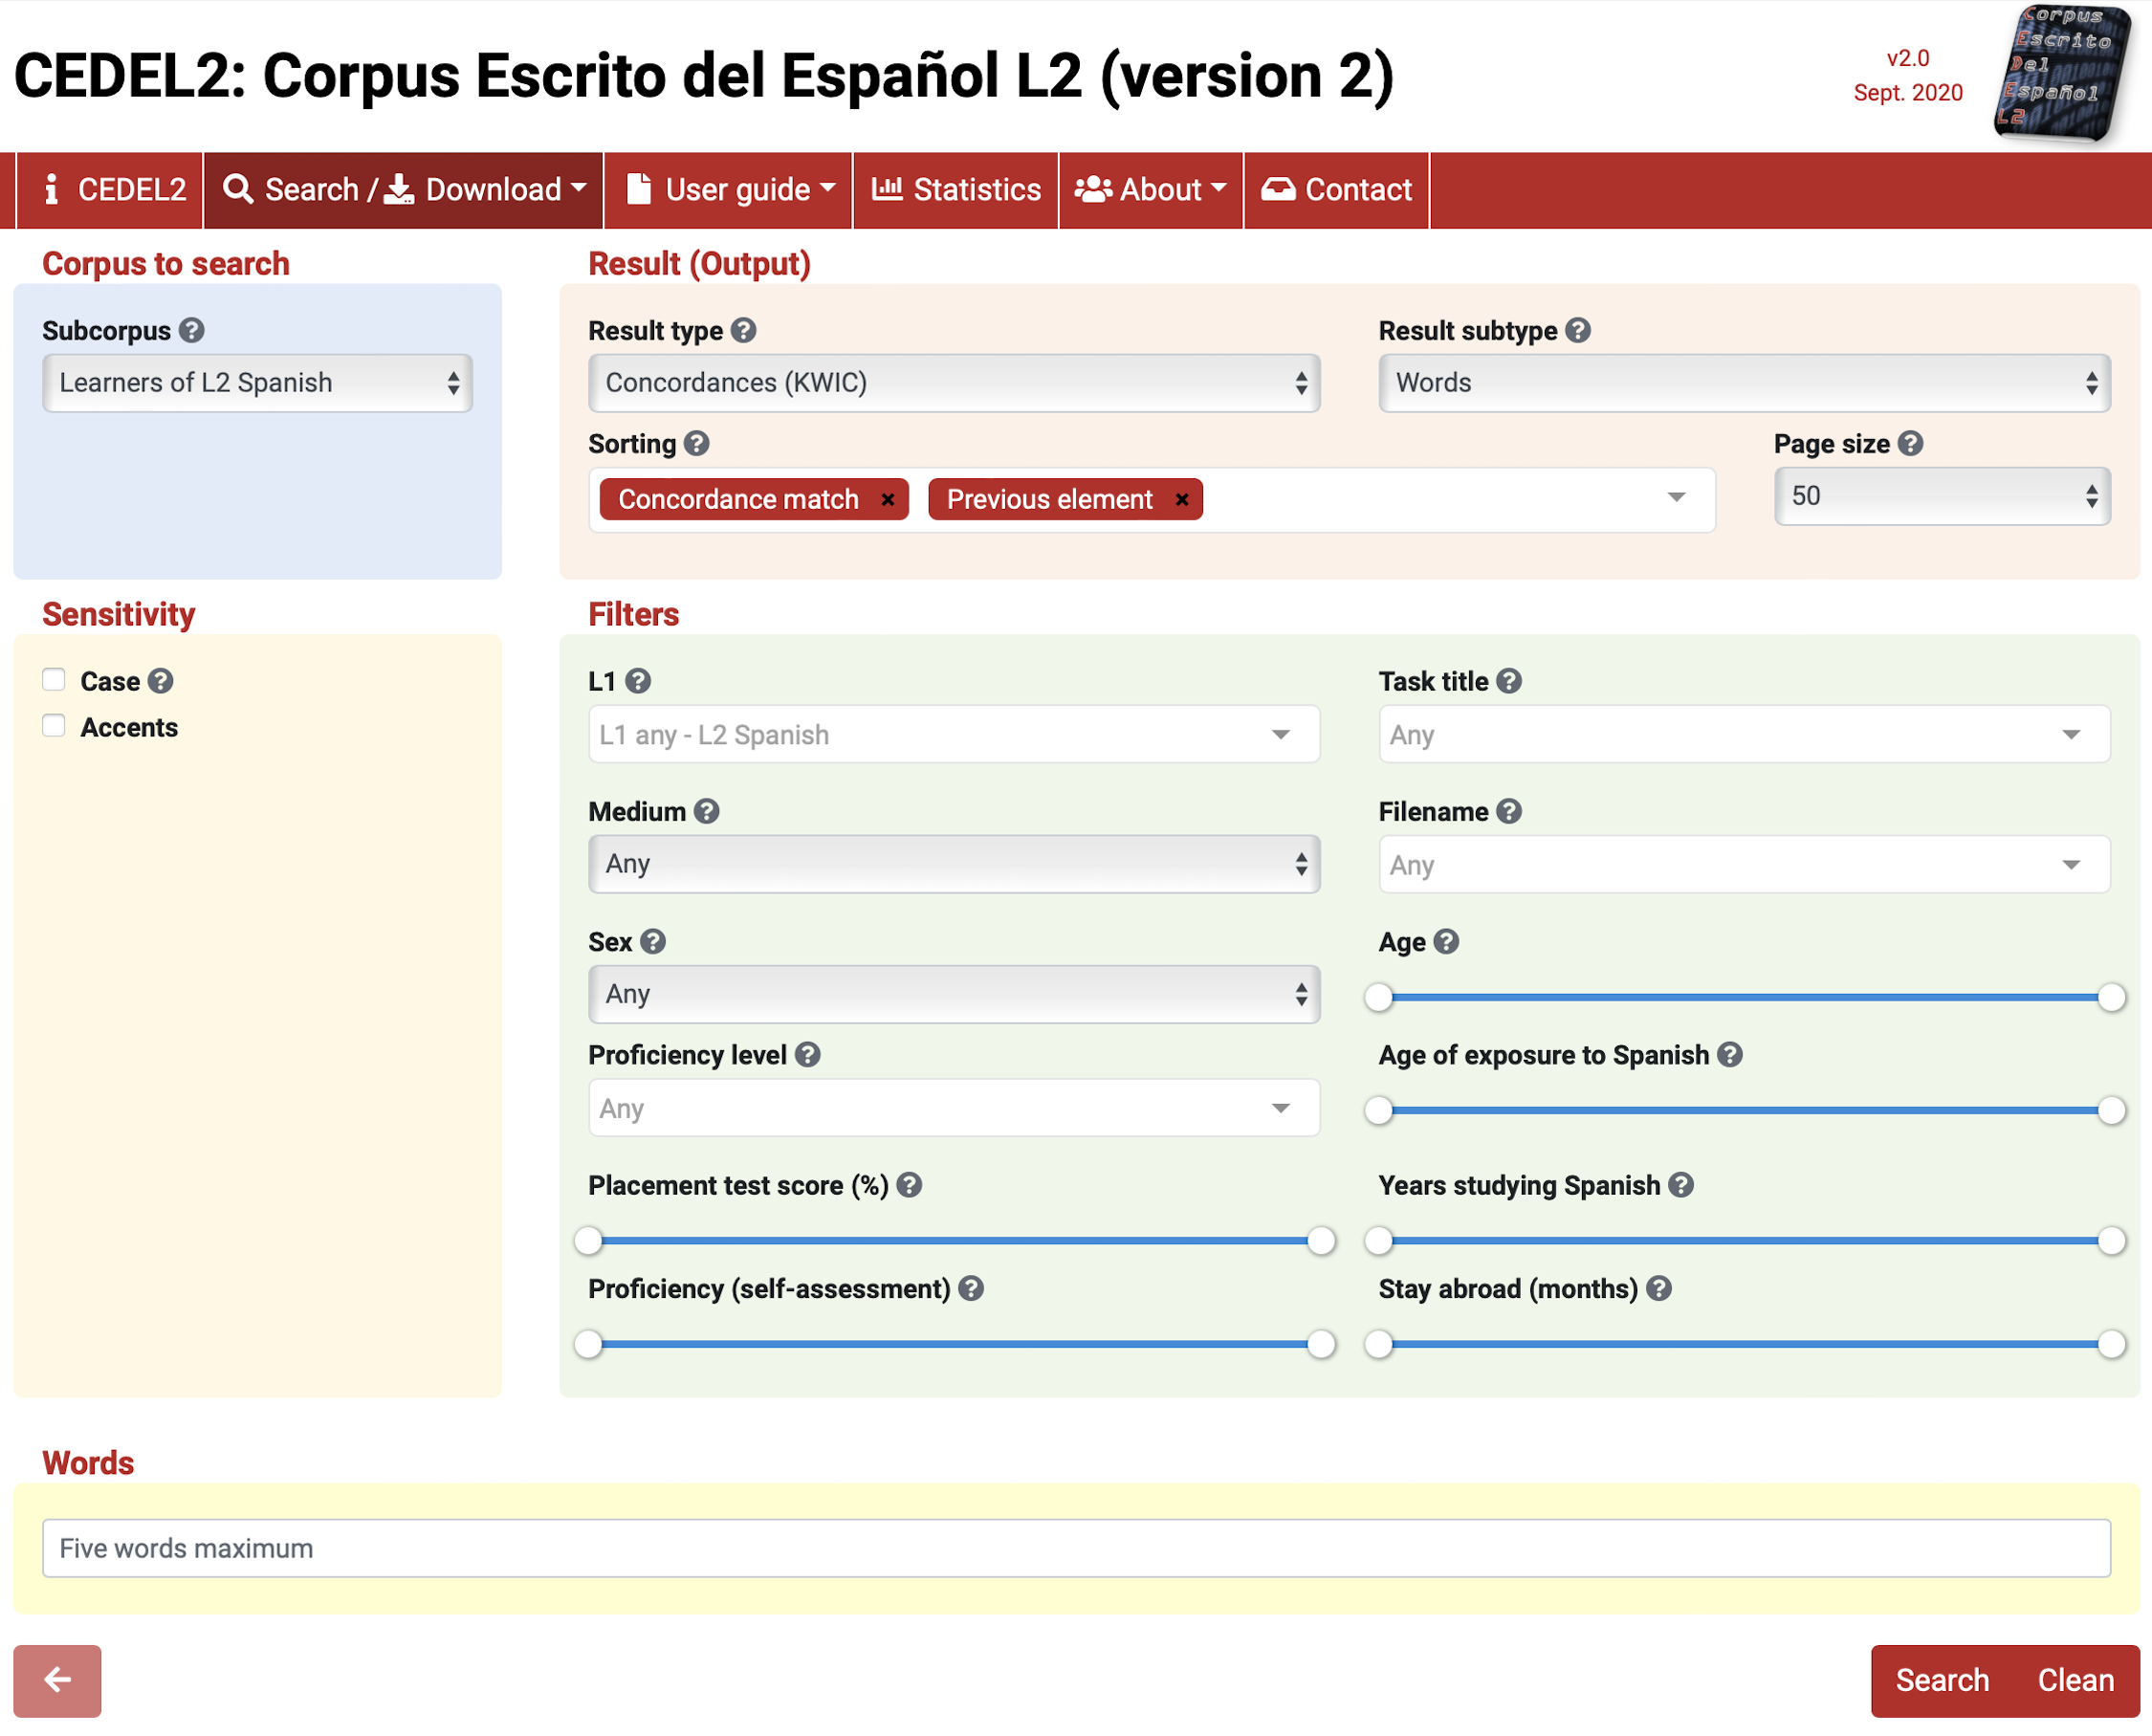
\includegraphics{part_3/figures/acquire-cedel2-search.png}

}

\caption{\label{fig-acquire-cedel2-search}Search and download interface
for the CEDEL2 Corpus}

\end{figure}%

For this example let's assume that we want to acquire data to use in a
study comparing the use of the Spanish preterite and imperfect past
tense aspect in written texts by English L1 learners of Spanish to
native Spanish speakers. To acquire data for such a project, we will
first select the subcorpus ``Learners of L2 Spanish''. We will set the
results to provide full texts and filter the results to ``L1 English -
L2 Spanish''. Additionally, we will set the medium to ``Written''. This
will provide us with a set of texts for the L2 learners that we can use
for our study. The search parameters and results are shown in
Figure~\ref{fig-acquire-cedel2-results}.

\begin{figure}[!htb]

\centering{

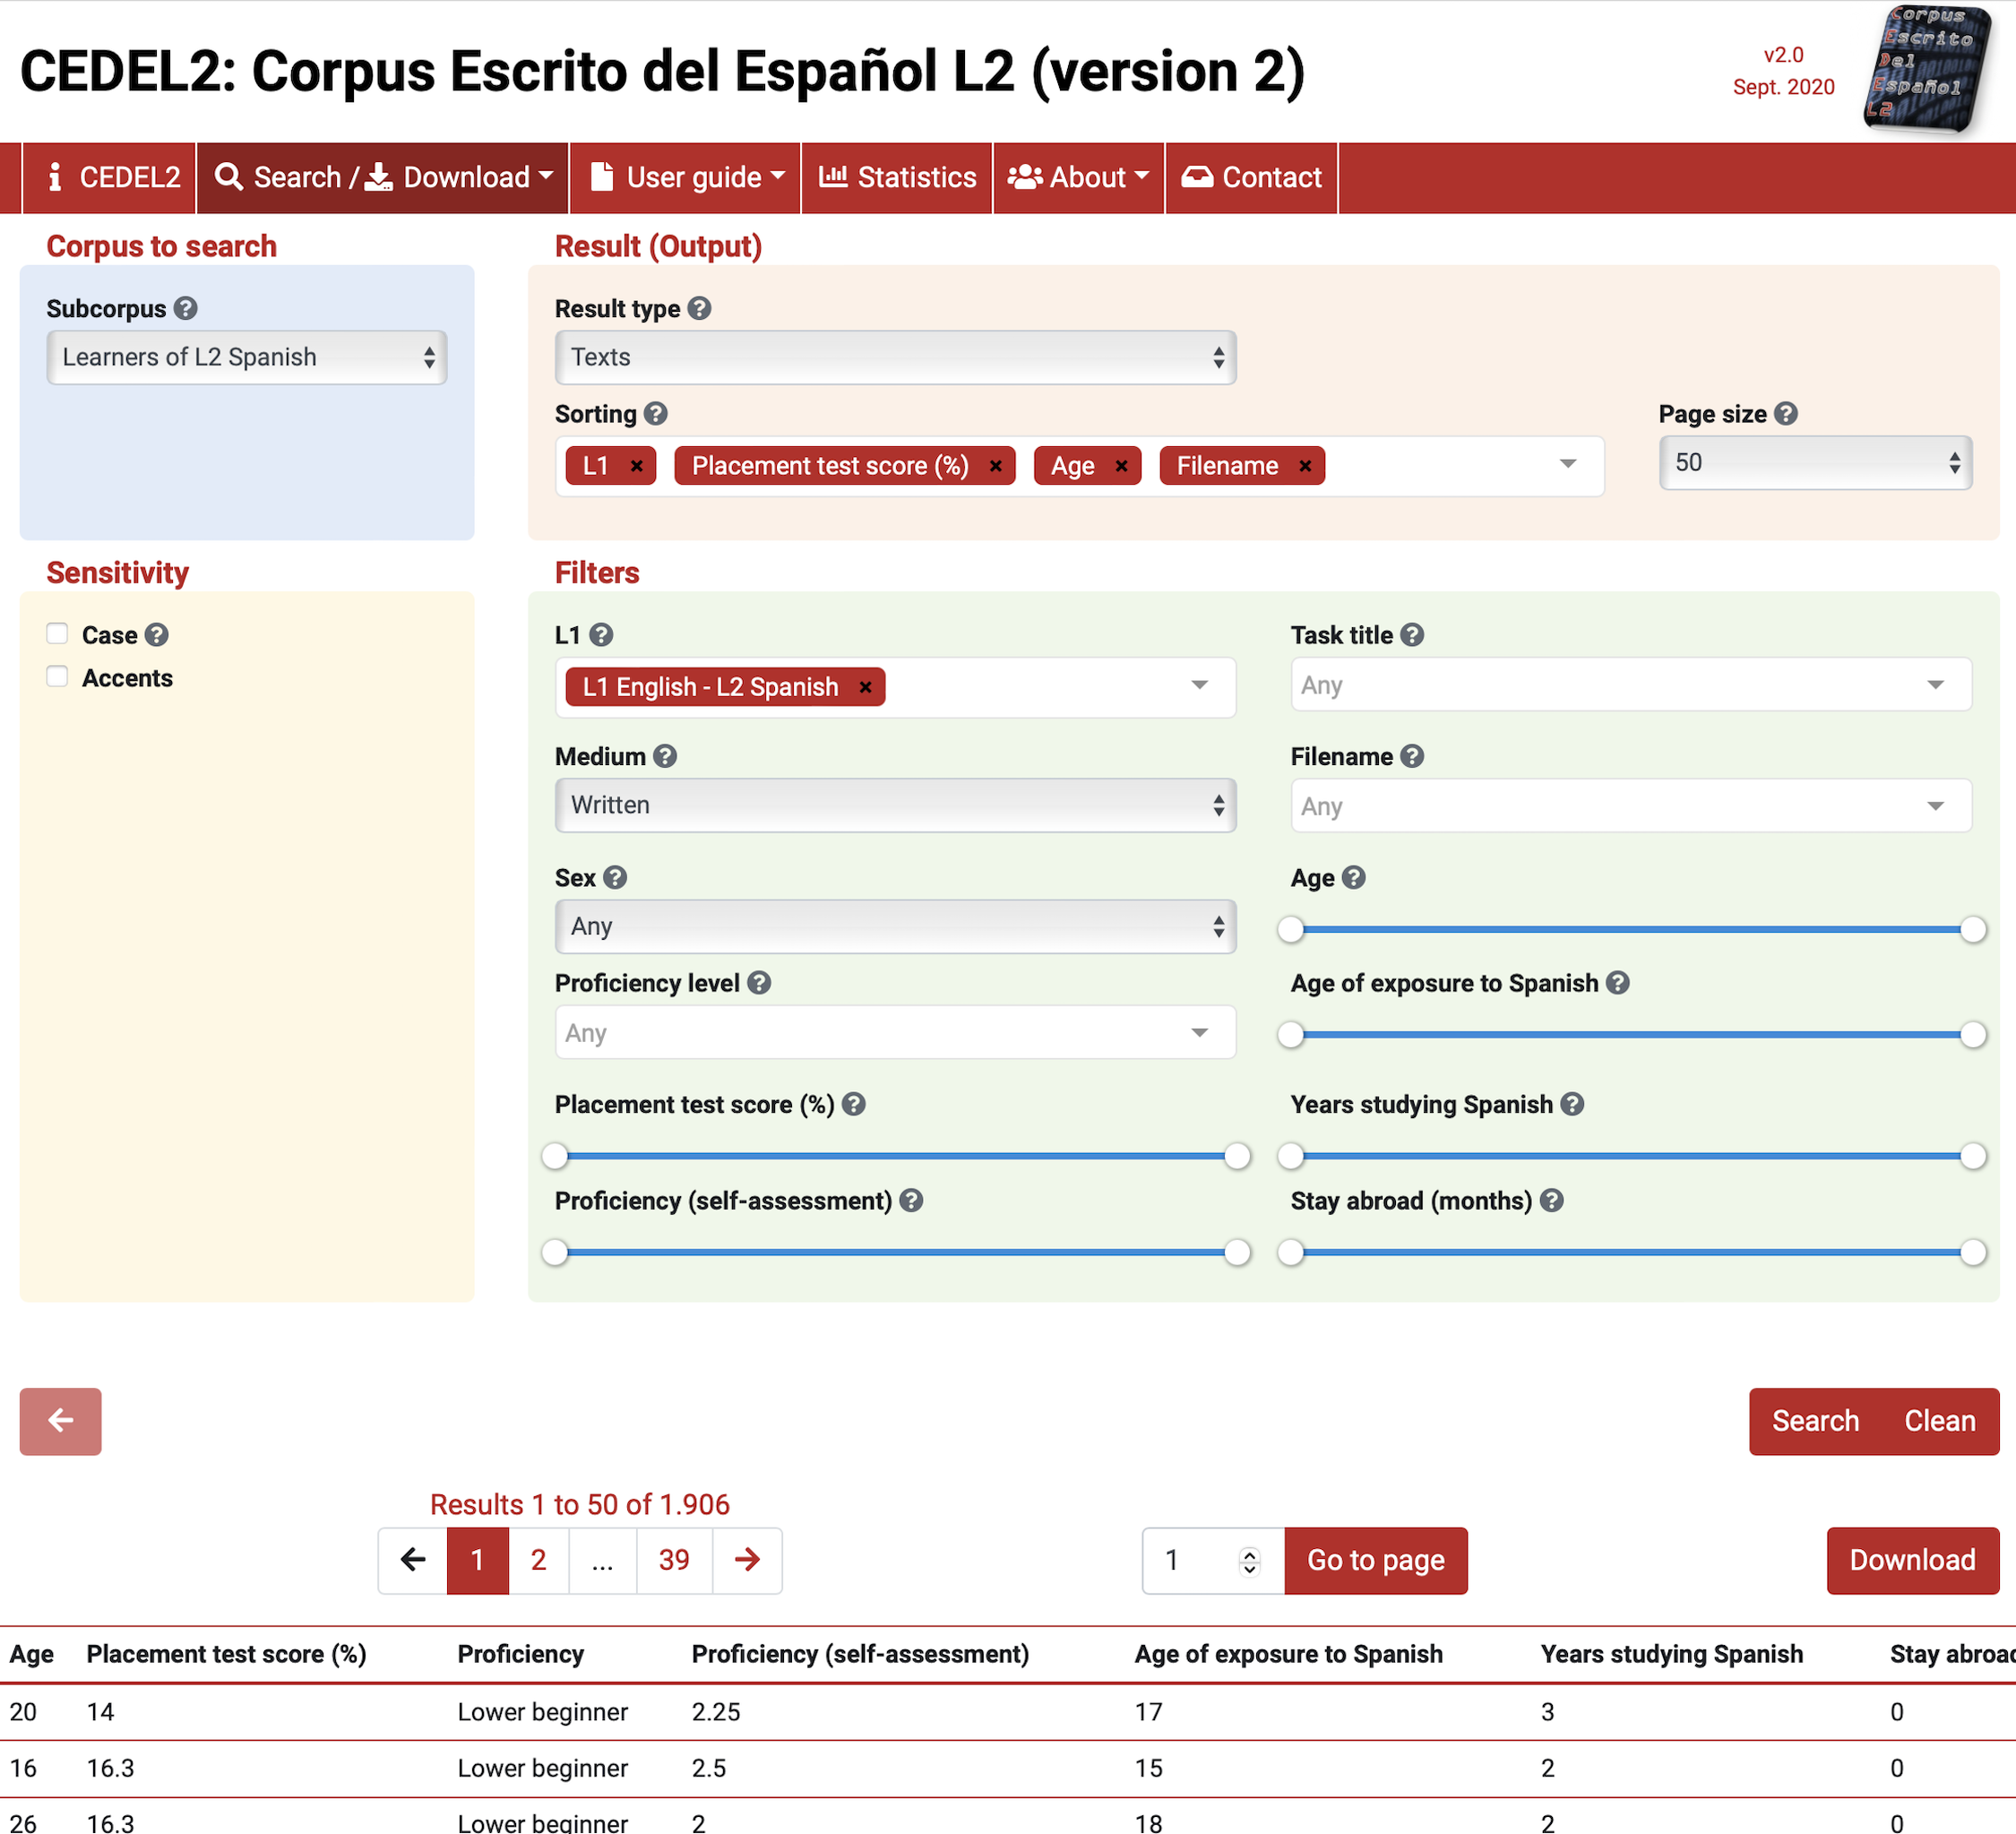
\includegraphics{part_3/figures/acquire-cedel2-results.png}

}

\caption{\label{fig-acquire-cedel2-results}Search results for the CEDEL2
Corpus}

\end{figure}%

The `Download' link now appears for this search criteria. Following this
link will provide the user a form to fill out. This particular resource
allows for access to different formats to download (Texts only, Texts
with metadata, CSV (Excel), CSV (Others)). I will select the `CSV
(Others)' option so that the data is structured for easier processing
downstream in subsequent processing steps. Then I save the CSV in the
\emph{data/original/} directory of my project and create a sub-directory
named \emph{cedel2/}, as seen in
Snippet~\ref{lst-acquire-cedel2-learners-download}.

\begin{codelisting}

\caption{\label{lst-acquire-cedel2-learners-download}Project structure
for the CEDEL2 corpus learner data download}

\centering{

\begin{Shaded}
\begin{Highlighting}[]
\ExtensionTok{data/}
\ExtensionTok{├──}\NormalTok{ analysis/}
\ExtensionTok{├──}\NormalTok{ derived/}
\ExtensionTok{└──}\NormalTok{ original/}
    \ExtensionTok{└──}\NormalTok{ cedel2/}
    \ExtensionTok{└──}\NormalTok{ cedel2{-}l1{-}english{-}learners.csv}
\end{Highlighting}
\end{Shaded}

}

\end{codelisting}%

Note that the file is named \emph{cedel2-l1-english-learners.csv} to
reflect the search criteria used to acquire the data. In combination
with other data documentation, this will help us to maintain
transparency.

Now, after downloading the L2 learner and the native speaker data into
the appropriate directory, we move on to the next processing step,
right? Not so fast! Imagine we are working on a project with a
collaborator. How will they know where the data came from? What if we
need to come back to this data in the future? How will we know what
characteristics we used to filter the data? The directory and filenames
may not be enough. To address these questions we need to document the
origin of the data, and in the case of data acquired through manual
downloads, we need to document the procedures we took to acquire the
data to the best of our ability.

\begin{tcolorbox}[enhanced jigsaw, left=2mm, toprule=.15mm, colback=white, colframe=quarto-callout-color-frame, arc=.35mm, rightrule=.15mm, bottomrule=.15mm, leftrule=.75mm, breakable, opacityback=0]

\textbf{\faIcon{hand-point-up} Tip}

There are many ways to create and edit CSV files. You can use a
spreadsheet program like MS Excel or Google Sheets, a text editor like
Notepad or TextEdit, or a code editor like RStudio or VS Code. The
\{qtkit\} package provides a convenient function,
\texttt{create\_data\_origin()} to create a CSV file with the data
origin boilerplate structure. This CSV file then can be edited to add
the relevant information in any of the above mentioned programs.

Using a spreadsheet program is the easiest method for editing tabular
data. The key is to save the file as a CSV file, and not as an Excel
file, to maintain our adherence to the principle of using open formats
for reproducible research.

\end{tcolorbox}

As discussed in Section~\ref{sec-data-data-origin}, all acquired data
should be accompanied by a data origin file. The majority of this
information can typically be identified on the resource's website and/
or the resource's documentation. In the case of the CEDEL2 corpus, the
corpus homepage provides most of the information we need.

Structurally, data documentation files should be stored close to the
data they describe. So for our data origin file this means adding it to
the \emph{data/original/} directory. Naming the file in a transparent
way is also important. I've named the file \emph{cedel2\_do.csv} to
reflect the name of the corpus, the meaning of the file as data origin
with a suffixed *\_do\emph{, and the file extension }.csv* to reflect
the file format. CSV files reflect tabular content. It is not required
that data origin files are tabular, but it makes it easier to read and
display them in literate programming documents.

In Table~\ref{tbl-acquire-cedel2-do}, I've created a data origin file
for the CEDEL2 corpus.

\begin{longtable}[]{@{}
  >{\raggedright\arraybackslash}p{(\columnwidth - 2\tabcolsep) * \real{0.2500}}
  >{\raggedright\arraybackslash}p{(\columnwidth - 2\tabcolsep) * \real{0.7500}}@{}}

\caption{\label{tbl-acquire-cedel2-do}Data origin file for the CEDEL2
corpus}

\tabularnewline

\toprule\noalign{}
\begin{minipage}[b]{\linewidth}\raggedright
attribute
\end{minipage} & \begin{minipage}[b]{\linewidth}\raggedright
description
\end{minipage} \\
\midrule\noalign{}
\endhead
\bottomrule\noalign{}
\endlastfoot
Resource name & CEDEL2: Corpus Escrito del Español como L2. \\
Data source & http://cedel2.learnercorpora.com/,
https://doi.org/10.1177/02676583211050522 \\
Data sampling frame & Corpus that contains samples of the language
produced from learners of Spanish as a second language. For comparative
purposes, it also contains a native control subcorpus of the language
produced by native speakers of Spanish from different varieties
(peninsular Spanish and all varieties of Latin American Spanish), so it
can be used as a native corpus in its own right. \\
Data collection date(s) & 2006-2020. \\
Data format & CSV file. Each row corresponds to a writing sample. Each
column is an attribute of the writing sample. \\
Data schema & A CSV file for L2 learners and a CSV file for native
speakers. \\
License & CC BY-NC-ND 3.0 ES \\
Attribution & Lozano, C. (2022). CEDEL2: Design, compilation and web
interface of an online corpus for L2 Spanish acquisition research.
Second Language Research, 38(4), 965-983.
https://doi.org/10.1177/02676583211050522. \\

\end{longtable}

Given this is a manual download we also need to document the procedure
used to retrieve the data in prose. The script in the \emph{process/}
directory that is typically used to acquire the data is not used to
programmatically retrieve data in this case. However, to keep things
predictable we will use this file to document the download procedure.
I've created a Quarto file named \emph{1\_acquire\_data.qmd} in the
\emph{process/} directory of my project.

A glimpse at the directory structure of the project at this point is
seen in Snippet~\ref{lst-acquire-cedel2-structure}.

\begin{codelisting}

\caption{\label{lst-acquire-cedel2-structure}Project structure for the
CEDEL2 corpus data acquisition}

\centering{

\begin{Shaded}
\begin{Highlighting}[]
\ExtensionTok{project/}
\ExtensionTok{├──}\NormalTok{ process/}
\ExtensionTok{│}\NormalTok{   ├── 1\_acquire\_data.qmd}
\ExtensionTok{│}\NormalTok{   └── ...}
\ExtensionTok{├──}\NormalTok{ data/}
\ExtensionTok{│}\NormalTok{   ├── analysis/}
\ExtensionTok{│}\NormalTok{   ├── derived/}
\ExtensionTok{│}\NormalTok{   └── original/}
\ExtensionTok{│}\NormalTok{       ├── cedel2\_do.csv}
\ExtensionTok{│}\NormalTok{       └── cedel2/}
\ExtensionTok{│}\NormalTok{           ├── cedel2{-}l1{-}english{-}learners.csv}
\ExtensionTok{│}\NormalTok{           └── cedel2{-}native{-}spanish{-}speakers.csv}
\ExtensionTok{├──}\NormalTok{ reports/}
\ExtensionTok{├──}\NormalTok{ DESCRIPTION}
\ExtensionTok{├──}\NormalTok{ Makefile}
\ExtensionTok{└──}\NormalTok{ README}
\end{Highlighting}
\end{Shaded}

}

\end{codelisting}%

Even though the \emph{1\_acquire\_data.qmd} file is not used to
programmatically retrieve the data, it is still a useful place to
document the download procedure. This includes the URL of the resource,
the search criteria used to filter the data, and the file format and
location of the data. It is also good to include and display your data
origin file in this file as a formatted table.

Manually downloading other resources will inevitably include unique
processes for obtaining the data, but in the end the data should be
archived in the project structure in the \emph{data/original/} directory
and documented in the appropriate places. Note that acquired data is
always treated as `read-only', meaning it is not modified in any way.
This gives us a fixed starting point for subsequent steps in the data
preparation process.

\subsection{Programmatic}\label{programmatic}

There are many resources that provide corpus data that is directly
accessible for which programmatic downloads can be applied. A
\textbf{programmatic download} is a download in which the process can be
automated through code. Thus, this is a reproducible process. The data
can be acquired by anyone with access to the necessary code.

In this case, and subsquent data acquisition procedures in this chapter,
we use the \emph{1\_acquire\_data.qmd} Quarto file to its full potential
intermingling prose, code, and code comments to execute and document the
download procedure.

To illustrate how this works to conduct a programmatic download, we will
work with the Switchboard Dialog Act Corpus (SWDA)
(\citeproc{ref-SWDA2008}{University of Colorado Boulder, 2008}). The
version that we will use is found on the Linguistic Data Consortium
under the \href{https://catalog.ldc.upenn.edu/LDC97S62}{Switchboard-1
Release 2 Corpus}. The corpus and related documentation are linked on
the catalog page \url{https://catalog.ldc.upenn.edu/docs/LDC97S62/}.

From the documentation we learn that the corpus contains transcripts for
1155 5-minute two-way telephone conversations among English speakers for
all areas of the United States. The speakers were given a topic to
discuss and the conversations were recorded. The corpus metadata and
annotations for sociolinguistic and discourse features.

This corpus, as you can image, could support a wide range of interesting
reseach questions. Let's assume we are following research conducted by
Tottie (\citeproc{ref-Tottie2011}{2011}) to explore the use of filled
pauses such as ``um'' and ``uh'' and traditional sociolinguistic
variables such as sex, age, and education in spontaneous speech by
American English speakers.

\begin{tcolorbox}[enhanced jigsaw, left=2mm, toprule=.15mm, colback=white, colframe=quarto-callout-color-frame, arc=.35mm, rightrule=.15mm, bottomrule=.15mm, leftrule=.75mm, breakable, opacityback=0]

\textbf{\faIcon{medal} Dive deeper}

You may be wondering what the difference betwen \emph{.zip},
\emph{.tar}, and \emph{.tar.gz} files are. The \emph{.zip} file format
is the most common. It groups file and directories into one file (an
archive) and compresses it to reduce the size of the file in one step
when the file is created.

The \emph{.tar} file format is used archive files and folders, it does
not perform compression. Gzipping peforms the compression to the
\emph{.tar} file resulting in a file with the \emph{.tar.gz} extension.
Notably the \emph{.gz} compression is highly efficient for large files.
Take the \emph{swda.tar.gz} file for example. It has a compressed file
size of 4.6 MB, but when uncompressed it is 16.9 MB. This is a 73\%
reduction in file size.

\end{tcolorbox}

With this goal in mind, let's get started writing the code to download
and organize the data in our project directory. First, we need to
identify the URL (Uniform Resource Locator) for the data that we want to
download. More often than not this file will be some type of archive
file with an extension such as \emph{.zip} (Zipped file), \emph{.tar}
(Tarball file), or \emph{tar.gz} (Gzipped tarball file), which is the
case for the SWDA corpus. Archive files make downloading multiple files
easy by grouping files and directories into one file.

In R, we can use the \texttt{download.file()} function from base R. The
\texttt{download.file()} function minimally requires two arguments:
\texttt{url} and \texttt{destfile}. These correspond to the file to
download and the location where it is to be saved to disk. To break out
the process a bit, I will assign the URL and destination file path to
variables and then use the \texttt{download.file()} function to download
the file.

\begin{example}[]\protect\hypertarget{exm-acquire-swda-download-file}{}\label{exm-acquire-swda-download-file}

~

\begin{Shaded}
\begin{Highlighting}[]
\CommentTok{\# URL to SWDA corpus archive file}
\NormalTok{file\_url }\OtherTok{\textless{}{-}}
  \StringTok{"https://catalog.ldc.upenn.edu/docs/LDC97S62/swb1\_dialogact\_annot.tar.gz"}

\CommentTok{\# Relative path to project/data/original directory}
\NormalTok{file\_path }\OtherTok{\textless{}{-}} \StringTok{"../data/original/swda.tar.gz"}

\CommentTok{\# Download SWDA corpus archive file}
\FunctionTok{download.file}\NormalTok{(}\AttributeTok{url =}\NormalTok{ file\_url, }\AttributeTok{destfile =}\NormalTok{ file\_path)}
\end{Highlighting}
\end{Shaded}

\end{example}

\begin{tcolorbox}[enhanced jigsaw, left=2mm, toprule=.15mm, colback=white, colframe=quarto-callout-color-frame, arc=.35mm, rightrule=.15mm, bottomrule=.15mm, leftrule=.75mm, breakable, opacityback=0]

\textbf{\faIcon{exclamation-triangle} Warning}

Note that the \texttt{file\_path} variable in
Example~\ref{exm-acquire-swda-download-file} is a relative path to the
\emph{data/original/} directory. This is because the
\emph{1\_acquire\_data.qmd} file that we are using for this code is
located in the \emph{process/} directory and the \emph{data/} directory
is a sibling directory to the \emph{process/} directory.

It is also possible to use an absolute path to the \emph{data/original/}
directory. I will have more to say about the advantages and
disadvantages of relative and absolute paths in reproducible research in
Chapter~\ref{sec-contribute-chapter}.

\end{tcolorbox}

As we can see looking at the directory structure, in
Snippet~\ref{lst-acquire-swda-download-location}, the
\emph{swda.tar.zip} file has been added to the \emph{data/original/}
directory.

\begin{codelisting}

\caption{\label{lst-acquire-swda-download-location}Project structure for
the SWDA archive file download}

\centering{

\begin{Shaded}
\begin{Highlighting}[]
\ExtensionTok{data/}
\ExtensionTok{├──}\NormalTok{ analysis/}
\ExtensionTok{├──}\NormalTok{ derived/}
\ExtensionTok{└──}\NormalTok{ original/}
    \ExtensionTok{└──}\NormalTok{ swda.tar.zip}
\end{Highlighting}
\end{Shaded}

}

\end{codelisting}%

Once an archive file is downloaded, however, the file needs to be
`unarchived' to reveal the directory structure and files. To unarchive
this \emph{.tar.gz} file we use the \texttt{untar()} function with the
arguments \texttt{tarfile} pointing to the \emph{.tar.gz} file and
\texttt{exdir} specifying the directory where we want the files to be
extracted to. Again, I will assign the arguments to variables. Then we
can unarchive the file using the \texttt{untar()} function.

\begin{example}[]\protect\hypertarget{exm-acquire-swda-archive-file}{}\label{exm-acquire-swda-archive-file}

~

\begin{Shaded}
\begin{Highlighting}[]
\CommentTok{\# Relative path to the archive file}
\NormalTok{tar\_file }\OtherTok{\textless{}{-}} \StringTok{"../data/original/swda.tar.gz"}

\CommentTok{\# Relative path to the directory to extract to}
\NormalTok{extract\_to\_dir }\OtherTok{\textless{}{-}} \StringTok{"../data/original/swda/"}

\CommentTok{\# Unarchive/ decompress .zip file and extract to our target directory}
\FunctionTok{untar}\NormalTok{(tar\_file, extract\_to\_dir)}
\end{Highlighting}
\end{Shaded}

\end{example}

The directory structure of \emph{data/} in
Snippet~\ref{lst-acquire-swda-unarchive-location} now shows the
\emph{swda.tar.gz} file and the \emph{swda} directory that contains the
unarchived directories and files.

\begin{codelisting}

\caption{\label{lst-acquire-swda-unarchive-location}Project structure
for the SWDA files unarchived}

\centering{

\begin{Shaded}
\begin{Highlighting}[]
\ExtensionTok{data/}
\ExtensionTok{├──}\NormalTok{ analysis/}
\ExtensionTok{├──}\NormalTok{ derived/}
\ExtensionTok{└──}\NormalTok{ original/}
    \ExtensionTok{├──}\NormalTok{ swda/}
    \ExtensionTok{│}\NormalTok{   ├── README}
    \ExtensionTok{│}\NormalTok{   ├── doc/}
    \ExtensionTok{│}\NormalTok{   ├── sw00utt/}
    \ExtensionTok{│}\NormalTok{   ├── sw01utt/}
    \ExtensionTok{│}\NormalTok{   ├── sw02utt/}
    \ExtensionTok{│}\NormalTok{   ├── sw03utt/}
    \ExtensionTok{│}\NormalTok{   ├── sw04utt/}
    \ExtensionTok{│}\NormalTok{   ├── sw05utt/}
    \ExtensionTok{│}\NormalTok{   ├── sw06utt/}
    \ExtensionTok{│}\NormalTok{   ├── sw07utt/}
    \ExtensionTok{│}\NormalTok{   ├── sw08utt/}
    \ExtensionTok{│}\NormalTok{   ├── sw09utt/}
    \ExtensionTok{│}\NormalTok{   ├── sw10utt/}
    \ExtensionTok{│}\NormalTok{   ├── sw11utt/}
    \ExtensionTok{│}\NormalTok{   ├── sw12utt/}
    \ExtensionTok{│}\NormalTok{   └── sw13utt/}
    \ExtensionTok{└──}\NormalTok{ swda.tar.gz}
\end{Highlighting}
\end{Shaded}

}

\end{codelisting}%

At this point we have acquired the data programmatically and with this
code as part of our workflow anyone could run this code and reproduce
the same results.

The code as it is, however, is not ideally efficient. First, the
\emph{swda.tar.gz} file is not strictly needed after we unarchive it and
it occupies disk space, if we keep it. And second, each time we run this
code the file will be downloaded from the remote server and overwrite
the existing data. This leads to unnecessary data transfer and server
traffic and will overwrite the data if it already exists in our project
directory which could be problematic if the data changes on the remote
server. Let's tackle each of these issues in turn.

To avoid writing the \emph{swda.tar.gz} file to disk (long-term) we can
use the \texttt{tempfile()} function to open a temporary holding space
for the file in the computing environment. This space can then be used
to store the file, unarchive it, and then the temporary file will
automatically be deleted. We assign the temporary space to an R object
we will name \texttt{temp\_file} with the \texttt{tempfile()} function.
This object can now be used as the value of the argument
\texttt{destfile} in the \texttt{download.file()} function.

\begin{example}[]\protect\hypertarget{exm-acquire-swda-temp-file}{}\label{exm-acquire-swda-temp-file}

~

\begin{Shaded}
\begin{Highlighting}[]
\CommentTok{\# URL to SWDA corpus archive file}
\NormalTok{file\_url }\OtherTok{\textless{}{-}}
  \StringTok{"https://catalog.ldc.upenn.edu/docs/LDC97S62/swb1\_dialogact\_annot.tar.gz"}

\CommentTok{\# Create a temporary file space for our .tar.gz file}
\NormalTok{temp\_file }\OtherTok{\textless{}{-}} \FunctionTok{tempfile}\NormalTok{()}

\CommentTok{\# Download SWDA corpus archive file}
\FunctionTok{download.file}\NormalTok{(file\_url, temp\_file)}
\end{Highlighting}
\end{Shaded}

\end{example}

\begin{tcolorbox}[enhanced jigsaw, left=2mm, toprule=.15mm, colback=white, colframe=quarto-callout-color-frame, arc=.35mm, rightrule=.15mm, bottomrule=.15mm, leftrule=.75mm, breakable, opacityback=0]

\textbf{\faIcon{hand-point-up} Tip}

In Example~\ref{exm-acquire-swda-temp-file}, I've used the values stored
in the objects \texttt{file\_url} and \texttt{temp\_file} in the
\texttt{download.file()} function without specifying the argument names
--only providing the names of the objects. R will assume that values of
a function map to the ordering of the arguments. If your values do not
map to ordering of the arguments you are required to specify the
argument name and the value. To view the ordering of objects hit
\texttt{tab} after entering the function name or consult the function
documentation by prefixing the function name with \texttt{?} and hitting
\texttt{enter}.

\end{tcolorbox}

At this point our downloaded file is stored temporarily on disk and can
be accessed and unarchived to our target directory using
\emph{temp\_file} as the value for the argument \texttt{tarfile} from
the \texttt{untar()} function. I've assigned our target directory path
to \texttt{extract\_to\_dir} and used it as the value for the argument
\texttt{exdir}.

\begin{example}[]\protect\hypertarget{exm-acquire-swda-untar-temp}{}\label{exm-acquire-swda-untar-temp}

~

\begin{Shaded}
\begin{Highlighting}[]
\CommentTok{\# Assign our target directory to \textasciigrave{}extract\_to\_dir\textasciigrave{}}
\NormalTok{extract\_to\_dir }\OtherTok{\textless{}{-}} \StringTok{"../data/original/swda/"}

\CommentTok{\# Unarchive/ decompress .tar.gz file and extract to our target directory}
\FunctionTok{untar}\NormalTok{(}\AttributeTok{tarfile =}\NormalTok{ temp\_file, }\AttributeTok{exdir =}\NormalTok{ target\_dir)}
\end{Highlighting}
\end{Shaded}

\end{example}

Our directory structure in Example~\ref{exm-acquire-swda-untar-temp} is
the same as in Snippet~\ref{lst-acquire-swda-unarchive-location}, minus
the \emph{swda.tar.gz} file.

The second issue I raised concerns the fact that running this code as
part of our project will repeat the download each time our script is
run. Since we would like to be good citizens and avoid unnecessary
traffic on the web and avoid potential issues in overwriting data, it
would be nice if our code checked to see if we already have the data on
disk and if it exists, then skip the download, if not then download it.

The desired functionality we've described can be implemented using the
\texttt{if()} function. The \texttt{if()} function is one of a class of
functions known as control statements. \textbf{Control statments} allow
us to control the flow of our code by evaluating logical statements and
processing subsequent code based on the logical value it is passed as an
argument.

So in this case we want to evaluate whether the data directory exists on
disk. If it does then skip the download, if not, proceed with the
download. In combination with \texttt{else} which provides the `if not'
part of the statement, we have the following logical flow in
Example~\ref{exm-acquire-if-dir-exists}.

\begin{example}[]\protect\hypertarget{exm-acquire-if-dir-exists}{}\label{exm-acquire-if-dir-exists}

~

\begin{Shaded}
\begin{Highlighting}[]
\ControlFlowTok{if}\NormalTok{ (DIRECTORY\_EXISTS) \{}
  \CommentTok{\# Do nothing}
\NormalTok{\} }\ControlFlowTok{else}\NormalTok{ \{}
  \CommentTok{\# Download data}
\NormalTok{\}}
\end{Highlighting}
\end{Shaded}

\end{example}

We can simplify this statement by using the \texttt{!} operator which
negates the logical value of the statement it precedes. So if the
directory exists, \texttt{!DIRECTORY\_EXISTS} will return \texttt{FALSE}
and if the directory does not exist, \texttt{!DIRECTORY\_EXISTS} will
return \texttt{TRUE}. In other words, if the directory does not exist,
download the data. This is shown in
Example~\ref{exm-acquire-if-dir-exists-simplified}.

\begin{example}[]\protect\hypertarget{exm-acquire-if-dir-exists-simplified}{}\label{exm-acquire-if-dir-exists-simplified}

~

\begin{Shaded}
\begin{Highlighting}[]
\ControlFlowTok{if}\NormalTok{ (}\SpecialCharTok{!}\NormalTok{DIRECTORY\_EXISTS) \{}
  \CommentTok{\# Download data}
\NormalTok{\}}
\end{Highlighting}
\end{Shaded}

\end{example}

Now, to determine if a directory exists in our project directory we will
turn to \{fs\} (\citeproc{ref-R-fs}{Hester, Wickham, \& Csárdi, 2023}).
\{fs\} provides a set of functions for interacting with the file system,
including \texttt{dir\_exists()}. \texttt{dir\_exists()} takes a path to
a directory as an argument and returns the logical value, \texttt{TRUE},
if that directory exists, and \texttt{FALSE} if it does not.

We can use this function to evaluate whether the directory exists and
then use the \texttt{if()} function to process the subsequent code based
on the logical flow we set out in
Example~\ref{exm-acquire-if-dir-exists-simplified}. Applied to our
project, the code will look like
Example~\ref{exm-acquire-swda-if-dir-exists}.

\begin{example}[]\protect\hypertarget{exm-acquire-swda-if-dir-exists}{}\label{exm-acquire-swda-if-dir-exists}

~

\begin{Shaded}
\begin{Highlighting}[]
\CommentTok{\# Load the \{fs\} package}
\FunctionTok{library}\NormalTok{(fs)}

\CommentTok{\# URL to SWDA corpus archive file}
\NormalTok{file\_url }\OtherTok{\textless{}{-}}
  \StringTok{"https://catalog.ldc.upenn.edu/docs/LDC97S62/swb1\_dialogact\_annot.tar.gz"}

\CommentTok{\# Create a temporary file space for our .tar.gz file}
\NormalTok{temp\_file }\OtherTok{\textless{}{-}} \FunctionTok{tempfile}\NormalTok{()}

\CommentTok{\# Assign our target directory to \textasciigrave{}extract\_to\_dir\textasciigrave{}}
\NormalTok{extract\_to\_dir }\OtherTok{\textless{}{-}} \StringTok{"../data/original/swda/"}

\CommentTok{\# Check if our target directory exists}
\CommentTok{\# If it does not exist, download the file and extract it}
\ControlFlowTok{if}\NormalTok{ (}\SpecialCharTok{!}\FunctionTok{dir\_exists}\NormalTok{(extract\_to\_dir)) \{}
  \CommentTok{\# Download SWDA corpus archive file}
  \FunctionTok{download.file}\NormalTok{(file\_url, temp\_file)}

  \CommentTok{\# Unarchive/ decompress .tar.gz file and extract to our target directory}
  \FunctionTok{untar}\NormalTok{(}\AttributeTok{tarfile =}\NormalTok{ temp\_file, }\AttributeTok{exdir =}\NormalTok{ extract\_to\_dir)}
\NormalTok{\}}
\end{Highlighting}
\end{Shaded}

\end{example}

The code in Example~\ref{exm-acquire-swda-if-dir-exists} is added to the
\emph{1\_acquire\_data.qmd} file. When this file is run, the SWDA corpus
data will be downloaded and extracted to our project directory. If the
data already exists, the download will be skipped, just as we wanted.

Now, before we move on, we need to make sure to document the process.
Now that our Quarto document includes code we can review, explain, and
comment this process. And, as always, create a data origin file as with
the relevant information. The data origin file will be stored in the
\emph{data/original/} directory and the Quarto file will be stored in
the \emph{process/} directory.

We've leveraged R to automate the download and extraction of the data,
depending on the existence of the data in our project directory. But you
may be asking yourself, ``Can't I just navigate to the corpus page and
download the data manually myself?'' The simple answer is, ``Yes, you
can.'' The more nuanced answer is, ``Yes, but consider the trade-offs.''

The following scenarios highlight the some advantages to automating the
process. If you are acquiring data from multiple files, it can become
tedious to document the manual process for each file such that it is
reproducible. It's possible, but it's error prone.

Now, if you are collaborating with others, you will want to share this
data with them. It is very common to find data that has limited
restrictions for use in academic projects, but the most common
limitation is redistribution. This means that you can use the data for
your own research, but you cannot share it with others. If you plan on
publishing your project to a code repository to share the data as part
of your reproducible project, you would be violating the terms of use
for the data. By including the programmatic download in your project,
you can ensure that your collaborators can easily and effectively
acquire the data themselves and that you are not violating the terms of
use.

\section{APIs}\label{sec-apis}

A convenient alternative method for acquiring data in R is through
package interfaces to web services. These interfaces are built using R
code to make connections with resources on the web through
\textbf{Application Programming Interfaces} (APIs). Websites such as
Project Gutenberg, Twitter, Reddit, and many others provide APIs to
allow access to their data under certain conditions, some more limiting
for data collection than others. Programmers (like you!) in the R
community take up the task of wrapping calls to an API with R code to
make accessing that data from R convenient, and of course reproducible.

\begin{tcolorbox}[enhanced jigsaw, left=2mm, toprule=.15mm, colback=white, colframe=quarto-callout-color-frame, arc=.35mm, rightrule=.15mm, bottomrule=.15mm, leftrule=.75mm, breakable, opacityback=0]

\textbf{\faIcon{medal} Dive deeper}

Many, many web services provide API access. These APIs span all kinds of
data, from text to images to video to audio. Visit the
\href{https://publicapis.io/}{Public APIs website} to explore the
diversity of APIs available.

ROpenSci maintains a curated list of R packages that provide access to
data from web services. Visit the
\href{https://ropensci.org/packages/data-access/}{ROpenSci website} to
explore the packages available.

\end{tcolorbox}

In addition to popular public APIs, there are also APIs that provide
access to repositories and databases which are of particular interest to
linguists. For example, \href{http://wordbank.stanford.edu/}{Wordbank}
provides access to a large collection of child language corpora through
\{wordbankr\} (\citeproc{ref-R-wordbankr}{Braginsky, 2024}), and
\href{https://glottolog.org/}{Glottolog},
\href{https://wals.info/}{World Atlas of Language Structures} (WALS),
and \href{https://phoible.org/}{PHOIBLE} provide access to large
collections of language metadata that can be accessed through
\{lingtypology\} (\citeproc{ref-R-lingtypology}{Moroz, 2017}).

Let's work with an R package that provides access to the
\href{https://talkbank.org/}{TalkBank} database. The TalkBank project
(\citeproc{ref-Macwhinney2024}{Macwhinney, 2024}) contains a large
collection of spoken language corpora from various contexts:
conversation, child language, multilinguals, \emph{etc}. Resource
information, web interfaces, and links to download data in various
formats can be found by perusing individual resources linked from the
main page. However, \{TBDBr\} (\citeproc{ref-R-TBDBr}{Kowalski \&
Cavanaugh, 2022}) provides convenient access to corpora using R once a
corpus resource is identified.

The CABNC (\citeproc{ref-Albert2015}{Albert, de Ruiter, \& de Ruiter,
2015}) contains the
\href{http://www.natcorp.ox.ac.uk/docs/URG/BNCdes.html\#body.1_div.1_div.5_div.1}{demographically
sampled portion} of the spoken portion of the British National Corpus
(BNC) (\citeproc{ref-Leech1992}{Leech, 1992}).

Useful for a study aiming to research spoken British English, either in
isoloation or in comparison to American English (SWDA).

First, we need to install and load \{TBDBr\}, as in
Example~\ref{exm-acquire-load-pacman}.

\begin{example}[]\protect\hypertarget{exm-acquire-load-pacman}{}\label{exm-acquire-load-pacman}

~

\begin{Shaded}
\begin{Highlighting}[]
\CommentTok{\# Load the TBDBr package}
\FunctionTok{library}\NormalTok{(TBDBr)}
\end{Highlighting}
\end{Shaded}

\end{example}

\{TBDBr\} provides a set of common \texttt{get*()} functions for
acquiring data from the TalkBank corpus resources. These include:
\texttt{getParticipants()}, \texttt{getTranscripts()},
\texttt{getTokens()}, \texttt{getTokenTypes()}, and
\texttt{getUtterances()}.

\begin{tcolorbox}[enhanced jigsaw, left=2mm, toprule=.15mm, colback=white, colframe=quarto-callout-color-frame, arc=.35mm, rightrule=.15mm, bottomrule=.15mm, leftrule=.75mm, breakable, opacityback=0]

\textbf{\faIcon{hand-point-up} Tip} List functions and arguments

For any package loaded in your R session, you can list all of its
functions and datasets using the \texttt{ls()} function. For example,
\texttt{ls("package:TBDBr")} will list all of the functions and datasets
in \{TBDBr\}.

To view all of the arguments for a function, use the \texttt{args()}
function. For example, \texttt{args(getUtterances)} will list all of the
arguments for the \texttt{getUtterances()} function.

\end{tcolorbox}

For each of these function the first argument is \texttt{corpusName},
which is the name of the corpus resource as it appears in the TalkBank
database. The second argument is \texttt{corpora}, which takes a
character vector describing the path to the data. For the CABNC, these
arguments are \texttt{"ca"} and \texttt{c("ca",\ "CABNC")} respectively.
To determine these values, TBDBr provides the \texttt{getLegalValues()}
interactive function which allows you to interactively select the
repository name, corpus name, and transcript name, if necessary.

Another important aspect of these function is that they return data
frame objects. Since we are accessing data that is in a structured
database, this makes sense. However, we should always check the
documentation for the object type that is returned by function to be
aware of how to work with the data.

Let's start by retrieving the utterance data for the CABNC and preview
the data frame it returns using \texttt{glimpse()}.

\begin{example}[]\protect\hypertarget{exm-acquire-get-utterances}{}\label{exm-acquire-get-utterances}

~

\begin{Shaded}
\begin{Highlighting}[]
\CommentTok{\# Set corpus\_name and corpus\_path}
\NormalTok{corpus\_name }\OtherTok{\textless{}{-}} \StringTok{"ca"}
\NormalTok{corpus\_path }\OtherTok{\textless{}{-}} \FunctionTok{c}\NormalTok{(}\StringTok{"ca"}\NormalTok{, }\StringTok{"CABNC"}\NormalTok{)}

\CommentTok{\# Get utterance data}
\NormalTok{utterances }\OtherTok{\textless{}{-}}
  \FunctionTok{getUtterances}\NormalTok{(}
    \AttributeTok{corpusName =}\NormalTok{ corpus\_name,}
    \AttributeTok{corpora =}\NormalTok{ corpus\_path}
\NormalTok{    )}

\CommentTok{\# Preview the data}
\FunctionTok{glimpse}\NormalTok{(utterances)}
\end{Highlighting}
\end{Shaded}

\begin{verbatim}
Rows: 235,901
Columns: 10
$ filename  <list> "KB0RE000", "KB0RE000", "KB0RE000", "KB0RE000", "KB0RE000",~
$ path      <list> "ca/CABNC/KB0/KB0RE000", "ca/CABNC/KB0/KB0RE000", "ca/CABNC~
$ utt_num   <list> 0, 1, 2, 3, 4, 5, 6, 7, 8, 9, 10, 11, 12, 13, 14, 15, 16, 1~
$ who       <list> "PS002", "PS006", "PS002", "PS006", "PS002", "PS006", "PS00~
$ role      <list> "Unidentified", "Unidentified", "Unidentified", "Unidentifi~
$ postcodes <list> <NULL>, <NULL>, <NULL>, <NULL>, <NULL>, <NULL>, <NULL>, <NU~
$ gems      <list> <NULL>, <NULL>, <NULL>, <NULL>, <NULL>, <NULL>, <NULL>, <NU~
$ utterance <list> "You enjoyed yourself in America", "Eh", "did you", "Oh I c~
$ startTime <list> "0.208", "2.656", "2.896", "3.328", "5.088", "6.208", "8.32~
$ endTime   <list> "2.672", "2.896", "3.328", "5.264", "6.016", "8.496", "9.31~
\end{verbatim}

\end{example}

Inspecting the output from Example~\ref{exm-acquire-get-utterances}, we
see that the data frame contains 235,901 observations and 10 variables.

The summary provided by \texttt{glimpse()} also provides other useful
information. First, we see the data type of each variable.
Interestingly, the data type for each variable in the data frame is a
list object. Being that a list is two-dimensional data type, like a data
frame, we have two-dimensional data inside two-dimensional data. This is
known as a \textbf{nested structure}. We will work with nested
structures in more depth later, but for now it will suffice to say that
we would like to `unnest' these lists and reveal the list-contained
vector types at the data frame level.

To do this we will pass the \texttt{utterances} data frame to the,
appropriately named, \texttt{unnest()} function from \{tidyr\}
(\citeproc{ref-R-tidyr}{Wickham, Vaughan, \& Girlich, 2024}).
\texttt{unnest()} takes a data frame and a vector of variable names to
unnest, \texttt{cols\ =\ c()}. To unnest all variables, we will use the
\texttt{everything()} function from \{dplyr\} to select all variables at
once. We will use the result to overwrite the \texttt{utterances} object
with the unnested data frame.

\begin{example}[]\protect\hypertarget{exm-acquire-unnest}{}\label{exm-acquire-unnest}

~

\begin{Shaded}
\begin{Highlighting}[]
\CommentTok{\# Unnest the data frame}
\NormalTok{utterances }\OtherTok{\textless{}{-}}
\NormalTok{  utterances }\SpecialCharTok{|\textgreater{}}
  \FunctionTok{unnest}\NormalTok{(}\AttributeTok{cols =} \FunctionTok{everything}\NormalTok{())}

\CommentTok{\# Preview the data}
\FunctionTok{glimpse}\NormalTok{(utterances)}
\end{Highlighting}
\end{Shaded}

\begin{verbatim}
Rows: 235,901
Columns: 10
$ filename  <chr> "KB0RE000", "KB0RE000", "KB0RE000", "KB0RE000", "KB0RE000", ~
$ path      <chr> "ca/CABNC/KB0/KB0RE000", "ca/CABNC/KB0/KB0RE000", "ca/CABNC/~
$ utt_num   <dbl> 0, 1, 2, 3, 4, 5, 6, 7, 8, 9, 10, 11, 12, 13, 14, 15, 16, 17~
$ who       <chr> "PS002", "PS006", "PS002", "PS006", "PS002", "PS006", "PS002~
$ role      <chr> "Unidentified", "Unidentified", "Unidentified", "Unidentifie~
$ postcodes <lgl> NA, NA, NA, NA, NA, NA, NA, NA, NA, NA, NA, NA, NA, NA, NA, ~
$ gems      <lgl> NA, NA, NA, NA, NA, NA, NA, NA, NA, NA, NA, NA, NA, NA, NA, ~
$ utterance <chr> "You enjoyed yourself in America", "Eh", "did you", "Oh I co~
$ startTime <chr> "0.208", "2.656", "2.896", "3.328", "5.088", "6.208", "8.32"~
$ endTime   <chr> "2.672", "2.896", "3.328", "5.264", "6.016", "8.496", "9.312~
\end{verbatim}

\end{example}

The output from Example~\ref{exm-acquire-unnest} shows that the
variables are now one-dimensional vector types.

Returning to the information about our data frame from
\texttt{glimpse()}, the second thing to notice is we get a short preview
of the values for each variable. There are a couple things we can gleen
from this. One is that we can confirm or clarify the meaning of the
variable names by looking at the values. The other thing to consider is
whether the values show any patterns that may be worthy of more
scrutiny. For example, various variables appear to contain the same
values for each observation. For a variable like \texttt{filename}, this
is expected as the first values likely correspond to the same file.
However, for the variables \texttt{postcodes} and \texttt{gems} the
values are `NA'. This suggests that these variables may not contain any
useful information and we may want to remove them later.

For now, however, we want to acquire and store the data in its original
form (or as closely as possible). So now, we have acquired the
utterances data and have it in our R session as a data frame. To store
this data in a file, we will first need to consider the file format.
Data frames are tabular, so that gives us a few options.

Since we are working in R, we could store this data as an R object, in
the form of an RDS file. An RDS file is a binary file that can be read
back into R as an R object. This is a good option if we want to store
the data for use in R, but not if we want to share the data with others
or use it in other software. Another option is to store the data as a
spreadsheet file, such as XSLX (MS Excel). This may make viewing and
editing the contents more convenient, but it depends on the software
available to you and others. A third, more viable option, is to store
the data as a CSV file. CSV files are plain text files that can be read
and written by most software. This makes CSV files one of the most
popular for sharing tablular data. For this reason, we will store the
data as a CSV file.

\{readr\} provides the \texttt{write\_csv()} function for writing data
frames to CSV files. The first argument is the data frame to write, and
the second argument is the path to the file to write. Note, however,
that the directories in the path we specify need to exist. If they do
not, we will get an error.

In this case, I would like to write the file \emph{utterances.csv} to
the \emph{../data/original/cabnc/} directory. The original project
structure does not contain a \emph{cabnc/} directory, so I need to
create one. To do this, I will use \texttt{dir\_create()} from \{fs\}.

\begin{example}[]\protect\hypertarget{exm-acquire-write-csv}{}\label{exm-acquire-write-csv}

~

\begin{Shaded}
\begin{Highlighting}[]
\CommentTok{\# Create the target directory}
\FunctionTok{dir\_create}\NormalTok{(}\StringTok{"../data/original/cabnc/"}\NormalTok{)}

\CommentTok{\# Write the data frame to a CSV file}
\FunctionTok{write\_csv}\NormalTok{(utterances, }\StringTok{"../data/original/cabnc/utterances.csv"}\NormalTok{)}
\end{Highlighting}
\end{Shaded}

\end{example}

Chaining the steps covered in Examples \ref{exm-acquire-get-utterances},
\ref{exm-acquire-unnest}, and \ref{exm-acquire-write-csv}, we have a
succinct and legible code to acquire, adjust, and write utterances from
the CABNC in Example~\ref{exm-acquire-get-unnest-write-csv}.

\begin{example}[]\protect\hypertarget{exm-acquire-get-unnest-write-csv}{}\label{exm-acquire-get-unnest-write-csv}

~

\begin{Shaded}
\begin{Highlighting}[]
\CommentTok{\# Set corpus\_name and corpus\_path}
\NormalTok{corpus\_name }\OtherTok{\textless{}{-}} \StringTok{"ca"}
\NormalTok{corpus\_path }\OtherTok{\textless{}{-}} \FunctionTok{c}\NormalTok{(}\StringTok{"ca"}\NormalTok{, }\StringTok{"CABNC"}\NormalTok{)}

\CommentTok{\# Create the target directory}
\FunctionTok{dir\_create}\NormalTok{(}\StringTok{"../data/original/cabnc/"}\NormalTok{)}

\CommentTok{\# Get utterance data}
\FunctionTok{getUtterances}\NormalTok{(}
  \AttributeTok{corpusName =}\NormalTok{ corpus\_name,}
  \AttributeTok{corpora =}\NormalTok{ corpus\_path}
\NormalTok{) }\SpecialCharTok{|\textgreater{}}
  \FunctionTok{unnest}\NormalTok{(}\AttributeTok{cols =} \FunctionTok{everything}\NormalTok{()) }\SpecialCharTok{|\textgreater{}}
  \FunctionTok{write\_csv}\NormalTok{(}\StringTok{"../data/original/cabnc/utterances.csv"}\NormalTok{)}
\end{Highlighting}
\end{Shaded}

\end{example}

If our goal is just to acquire utterances, then we are done acquiring
data and we move on to the next step. However, if we want to acquire
other datasets from the CABNC, say participants, tokens, \emph{etc.},
then we can either repeat the steps in
Example~\ref{exm-acquire-get-unnest-write-csv} for each data type, or we
can write a function to do this for us!

A function serves us to make our code more legible and reusable for the
CABNC, and since the TalkBank data is structured similarly across
corpora, we can also use the function to acquire data from other
corpora, if need be.

To write a function, we need to consider the following:

\begin{enumerate}
\def\labelenumi{\arabic{enumi}.}
\tightlist
\item
  What is the name of the function?
\item
  What arguments does the function take?
\item
  What functionality does the function provide?
\item
  Does the function have optional arguments?
\item
  How does the function return the results?
\end{enumerate}

Taking each in turn, the name of the function should be descriptive of
what the function does. In this case, we are acquiring and writing data
from Talkbank corpora. A possible name is
\texttt{get\_talkbank\_data()}. The required arguments of the the
\texttt{get*()} functions will definitely figure in our function. In
addition, we will need to specify the path to the directory to write the
data. With these considerations, we can write the function signature in
Example~\ref{exm-acquire-get-talkbank-data-1}.

\begin{example}[]\protect\hypertarget{exm-acquire-get-talkbank-data-1}{}\label{exm-acquire-get-talkbank-data-1}

~

\begin{Shaded}
\begin{Highlighting}[]
\NormalTok{get\_talkbank\_data }\OtherTok{\textless{}{-}} \ControlFlowTok{function}\NormalTok{(corpus\_name, corpus\_path, target\_dir) \{}
  \CommentTok{\# ...}
\NormalTok{\}}
\end{Highlighting}
\end{Shaded}

\end{example}

The next thing to consider is what functionality the function provides.
In this case, we want to acquire and write data from Talkbank corpora.
We can start by leveraging the code steps in
Example~\ref{exm-acquire-get-unnest-write-csv}, making some adjustments
to the code replacing the hard-coded values with the function arguments
and adding code to create the target file name based on the
\texttt{target\_dir} argument.

\begin{example}[]\protect\hypertarget{exm-acquire-get-talkbank-data-2}{}\label{exm-acquire-get-talkbank-data-2}

~

\begin{Shaded}
\begin{Highlighting}[]
\NormalTok{get\_talkbank\_data }\OtherTok{\textless{}{-}} \ControlFlowTok{function}\NormalTok{(corpus\_name, corpus\_path, target\_dir) \{}

  \CommentTok{\# Create the target directory}
  \FunctionTok{dir\_create}\NormalTok{(target\_dir)}

  \CommentTok{\# Set up file path name}
\NormalTok{  utterances\_file  }\OtherTok{\textless{}{-}} \FunctionTok{path}\NormalTok{(target\_dir, }\StringTok{"utterances.csv"}\NormalTok{)}

  \CommentTok{\# Acquire data and write to file}
  \FunctionTok{getUtterances}\NormalTok{(}\AttributeTok{corpusName =}\NormalTok{ corpus\_name, }\AttributeTok{corpora =}\NormalTok{ corpus\_path) }\SpecialCharTok{|\textgreater{}}
    \FunctionTok{unnest}\NormalTok{(}\AttributeTok{cols =} \FunctionTok{everything}\NormalTok{()) }\SpecialCharTok{|\textgreater{}}
    \FunctionTok{write\_csv}\NormalTok{(utterances\_file)}
\NormalTok{\}}
\end{Highlighting}
\end{Shaded}

\end{example}

Before we address the obvious feature missing, which is the fact that
this function in Example~\ref{exm-acquire-get-talkbank-data-2} only
acquires and writes data for utterances, let's consider some
functionality which would make this function more user-friendly.

What if the data is already acquired? Do we want to overwrite it, or
should the function skip the process for files that already exist? By
skipping the process, we can save time and computing resources. If the
files are periodically updated, then we might want to overwrite existing
files.

To achieve this functionality we will use an \texttt{if()} statement to
check if the file exists. If it does, then we will skip the process. If
it does not, then we will acquire and write the data.

\begin{example}[]\protect\hypertarget{exm-acquire-get-talkbank-data-3}{}\label{exm-acquire-get-talkbank-data-3}

~

\begin{Shaded}
\begin{Highlighting}[]
\NormalTok{get\_talkbank\_data }\OtherTok{\textless{}{-}} \ControlFlowTok{function}\NormalTok{(corpus\_name, corpus\_path, target\_dir) \{}

  \CommentTok{\# Create the target directory}
  \FunctionTok{dir\_create}\NormalTok{(target\_dir)}

  \CommentTok{\# Set up file path name}
\NormalTok{  utterances\_file  }\OtherTok{\textless{}{-}} \FunctionTok{path}\NormalTok{(target\_dir, }\StringTok{"utterances.csv"}\NormalTok{)}

  \CommentTok{\# If the file does not exist, then...}
  \CommentTok{\# Acquire data and write to file}
  \ControlFlowTok{if}\NormalTok{(}\SpecialCharTok{!}\FunctionTok{file\_exists}\NormalTok{(utterances\_file)) \{}
    \FunctionTok{getUtterances}\NormalTok{(}\AttributeTok{corpusName =}\NormalTok{ corpus\_name, }\AttributeTok{corpora =}\NormalTok{ corpus\_path) }\SpecialCharTok{|\textgreater{}}
      \FunctionTok{unnest}\NormalTok{(}\AttributeTok{cols =} \FunctionTok{everything}\NormalTok{()) }\SpecialCharTok{|\textgreater{}}
      \FunctionTok{write\_csv}\NormalTok{(utterances\_file)}
\NormalTok{  \}}
\NormalTok{\}}
\end{Highlighting}
\end{Shaded}

\end{example}

We can also add functionality to
Example~\ref{exm-acquire-get-talkbank-data-3} to force overwrite
existing files, if need be. To do this, we will add an optional argument
to the function, \texttt{force}, which will be a logical value. We will
set the default to \texttt{force\ =\ FALSE} to preserve the existing
functionality. If \texttt{force\ =\ TRUE}, then we will overwrite
existing files. Then we add another condition to the \texttt{if()}
statement to check if \texttt{force\ =\ TRUE}. If it is, then we will
overwrite existing files.

\begin{example}[]\protect\hypertarget{exm-acquire-get-talkbank-data-4}{}\label{exm-acquire-get-talkbank-data-4}

~

\begin{Shaded}
\begin{Highlighting}[]
\NormalTok{get\_talkbank\_data }\OtherTok{\textless{}{-}} \ControlFlowTok{function}\NormalTok{(corpus\_name, corpus\_path, target\_dir, }\AttributeTok{force =} \ConstantTok{FALSE}\NormalTok{) \{}

  \CommentTok{\# Create the target directory}
  \FunctionTok{dir\_create}\NormalTok{(target\_dir)}

  \CommentTok{\# Set up file path name}
\NormalTok{  utterances\_file  }\OtherTok{\textless{}{-}} \FunctionTok{path}\NormalTok{(target\_dir, }\StringTok{"utterances.csv"}\NormalTok{)}

  \CommentTok{\# If the file does not exist, then...}
  \CommentTok{\# Acquire data and write to file}
  \ControlFlowTok{if}\NormalTok{(}\SpecialCharTok{!}\FunctionTok{file\_exists}\NormalTok{(utterances\_file) }\SpecialCharTok{|}\NormalTok{ force) \{}
    \FunctionTok{getUtterances}\NormalTok{(}\AttributeTok{corpusName =}\NormalTok{ corpus\_name, }\AttributeTok{corpora =}\NormalTok{ corpus\_path) }\SpecialCharTok{|\textgreater{}}
      \FunctionTok{unnest}\NormalTok{(}\AttributeTok{cols =} \FunctionTok{everything}\NormalTok{()) }\SpecialCharTok{|\textgreater{}}
      \FunctionTok{write\_csv}\NormalTok{(utterances\_file)}
\NormalTok{  \}}
\NormalTok{\}}
\end{Highlighting}
\end{Shaded}

\end{example}

From this point, we add the functionality to acquire and write the other
data available from Talkbank corpora, such as participants, tokens,
\emph{etc.} This involves adding additional file path names and
\texttt{if()} statements to check if the files exist surrounding the
processing steps to Example~\ref{exm-acquire-get-talkbank-data-4}. It
may be helpful to perform other input checks, print messages,
\emph{etc.} for functions that we plan to share with others. I will
leave these enhancements as an exercise for the reader.

\begin{tcolorbox}[enhanced jigsaw, left=2mm, toprule=.15mm, colback=white, colframe=quarto-callout-color-frame, arc=.35mm, rightrule=.15mm, bottomrule=.15mm, leftrule=.75mm, breakable, opacityback=0]

\textbf{\faIcon{medal} Dive deeper}

If you are interested in learning more about writing functions, check
out the \href{https://r4ds.had.co.nz/functions.html}{Writing Functions
chapter} in the \href{https://r4ds.had.co.nz/}{R for Data Science} book.

If you find yourself writing functions that are useful for multiple
projects, you may want to consider creating an R package. R packages are
a great way to share your code with others. If you are interested in
learning more about creating R packages, check out the
\href{https://r-pkgs.org/}{R Packages book} by Wickham \& Bryan
(\citeproc{ref-Wickham2023}{2023}).

\end{tcolorbox}

Before we leave the topic of functions, let's consider where to put
functions after we write them. Here are a few options:

\begin{enumerate}
\def\labelenumi{\arabic{enumi}.}
\tightlist
\item
  In the same script as the code that uses the function.
\item
  In a separate script, such as \emph{functions.R}.
\item
  In a package, which is loaded by the script that uses the function.
\end{enumerate}

The general heuristic for choosing where to put functions is to put them
in the same script as the code that uses them if the function is only
used in that script. If the function is used in multiple scripts or the
function or number of functions clutters the readability of the code,
then put it in a separate script. If the function is used in multiple
projects, then put it in an R package.

In this case, we will put the function in a separate file,
\emph{functions.R}, in the same directory as the other process files as
in Snippet~\ref{lst-acquire-functions-r}.

\begin{codelisting}

\caption{\label{lst-acquire-functions-r}Project structure with
\emph{functions.R} file}

\centering{

\begin{Shaded}
\begin{Highlighting}[]
\ExtensionTok{process/}
  \ExtensionTok{│}\NormalTok{   ├── 1\_acquire\_data.qmd}
  \ExtensionTok{│}\NormalTok{   ├── ...}
  \ExtensionTok{│}\NormalTok{   └── functions.R}
\end{Highlighting}
\end{Shaded}

}

\end{codelisting}%

\begin{tcolorbox}[enhanced jigsaw, left=2mm, toprule=.15mm, colback=white, colframe=quarto-callout-color-frame, arc=.35mm, rightrule=.15mm, bottomrule=.15mm, leftrule=.75mm, breakable, opacityback=0]

\textbf{\faIcon{exclamation-triangle} Warning}

Note that the \emph{functions.R} file is an R script, not a Quarto
document. Therefore code blocks that are used in \emph{.qmd} files are
not used, only the R code and code comments.

\end{tcolorbox}

To include this, or other functions in in the R session of the process
file that uses them, use the \texttt{source()} function, with the
correct relative path to the file, as seen in
Example~\ref{exm-acquire-source-functions}.

\begin{example}[]\protect\hypertarget{exm-acquire-source-functions}{}\label{exm-acquire-source-functions}

~

\begin{Shaded}
\begin{Highlighting}[]
\CommentTok{\# Source functions}
\FunctionTok{source}\NormalTok{(}\StringTok{"functions.R"}\NormalTok{)}
\end{Highlighting}
\end{Shaded}

\end{example}

It is common to source functions at the top of the process file as part
of the package setup.

Given the utility of this function to my projects and potentially
others', I've included the \texttt{get\_talkbank\_data()} function in
the \{qtkit\} package. You can view the source code by calling the
function without parentheses \texttt{()}, or on the \{qtkit\} GitHub
repository.

After running the \texttt{get\_talkbank\_data()} function, we can see
that the data has been acquired and written to the
\emph{data/original/cabnc/} directory in
Snippet~\ref{lst-acquire-functions-output}

\begin{codelisting}

\caption{\label{lst-acquire-functions-output}Project structure with
CABNC data files}

\centering{

\begin{Shaded}
\begin{Highlighting}[]
\ExtensionTok{data/}
\ExtensionTok{├──}\NormalTok{ analysis}
\ExtensionTok{├──}\NormalTok{ derived}
\ExtensionTok{└──}\NormalTok{ original}
    \ExtensionTok{└──}\NormalTok{ cabnc}
        \ExtensionTok{├──}\NormalTok{ participants.csv}
        \ExtensionTok{├──}\NormalTok{ token\_types.csv}
        \ExtensionTok{├──}\NormalTok{ tokens.csv}
        \ExtensionTok{├──}\NormalTok{ transcripts.csv}
        \ExtensionTok{└──}\NormalTok{ utterances.csv}
\end{Highlighting}
\end{Shaded}

}

\end{codelisting}%

Add comments to your code in \emph{1-acquire-data.qmd} and create and
complete the data origin documentation file for this resource, and the
acquisition is complete.

\section*{Activities}\label{activities-3}
\addcontentsline{toc}{section}{Activities}

\markright{Activities}

Building on the activities in the previous chapter, these activities
will focus on the implementation of the data acquisition process. Key
programming concepts include writing custom functions, control
statements, and applying functions iteratively will be covered in
addition to packages and functions which provide access to data from the
web.

\begin{tcolorbox}[enhanced jigsaw, left=2mm, toprule=.15mm, colback=white, colframe=quarto-callout-color-frame, arc=.35mm, rightrule=.15mm, bottomrule=.15mm, leftrule=.75mm, breakable, opacityback=0]

\textbf{\faIcon{file-code} Recipe}

\textbf{What}: Collecting and documenting data\\
\textbf{How}: Read Recipe 5, complete comprehension check, and prepare
for Lab 5.\\
\textbf{Why}: To refine programming strategies introduced in the lesson
for controlling program flow and making code more reusable in the
service of programmatically acquiring and documenting data.

\end{tcolorbox}

\begin{tcolorbox}[enhanced jigsaw, left=2mm, toprule=.15mm, colback=white, colframe=quarto-callout-color-frame, arc=.35mm, rightrule=.15mm, bottomrule=.15mm, leftrule=.75mm, breakable, opacityback=0]

\textbf{\faIcon{flask} Lab}

\textbf{What}: Harvesting research data\\
\textbf{How}: Fork, clone, and complete the steps in Lab 5.\\
\textbf{Why}: To investigate data sources, plan data collection
strategies, and apply skills and knowledge to use R to collect and
document data.

\end{tcolorbox}

\section*{Summary}\label{summary-4}
\addcontentsline{toc}{section}{Summary}

\markright{Summary}

In this chapter, we have covered a lot of ground. On the surface, we
have discussed a few methods for acquiring corpus data for use in text
analysis. In the process, we have delved into various aspects of the R
programming language. Some key concepts include writing control
statements and custom functions. We have also considered topics that are
more general in nature and concern interacting with data found on the
internet.

Each of these methods should be approached in a way that is transparent
to the researcher and to would-be collaborators and the general research
community. For this reason, the documentation of the steps taken to
acquire data are key both in the code and in human-facing documentation.

At this point you have both a bird's eye view of the data available on
the web and strategies on how to access a great majority of it. It is
now time to turn to the next step in our data analysis project: data
curation. In the next chapter, I will cover how to wrangle your raw data
into a tidy dataset.

\chapter{Curate}\label{sec-curate-chapter}

\begin{quote}
The hardest bit of information to extract is the first piece.

--- Robert Ferrigno
\end{quote}

\begin{tcolorbox}[enhanced jigsaw, left=2mm, toprule=.15mm, colback=white, colframe=quarto-callout-color-frame, arc=.35mm, rightrule=.15mm, bottomrule=.15mm, leftrule=.75mm, breakable, opacityback=0]

\textbf{\faIcon{list-alt} Outcomes}

\begin{itemize}
\tightlist
\item
  Describe the importance of data curation in text analysis
\item
  Recognize the different types of data formats
\item
  Associate the types data formats with the appropriate R programming
  techniques to curate the data
\end{itemize}

\end{tcolorbox}

In this chapter, we will now look at the next step in a text analysis
project: data curation. That is, the process of converting the original
data we acquire to a tidy dataset. Acquired data can come in a wide
variety of formats. These formats tend to signal the richness of the
metadata that is included in the file content. We will consider three
general types of content formats: (1) unstructured data, (2) structured
data, and (3) semi-structured data. Regardless of the file type and the
structure of the data, it will be necessary to consider how to curate a
dataset that such that the structure reflects the basic the unit of
analysis that we wish to investigate. The resulting dataset will form
the base from which we will work to further transform the dataset such
that it aligns with the unit(s) of observation required for the analysis
method that we will implement. Once the dataset is curated, we will
create a data dictionary that describes the dataset and the variables
that are included in the dataset for transparency and reproducibility.

\begin{tcolorbox}[enhanced jigsaw, left=2mm, toprule=.15mm, colback=white, colframe=quarto-callout-color-frame, arc=.35mm, rightrule=.15mm, bottomrule=.15mm, leftrule=.75mm, breakable, opacityback=0]

\textbf{\faIcon{terminal} Lessons}

\textbf{What}: Pattern Matching, Tidy Datasets\\
\textbf{How}: In an R console, load \{swirl\}, run \texttt{swirl()}, and
follow prompts to select the lesson.\\
\textbf{Why}: To familiarize yourself with the basics of using the
pattern matching syntax Regular Expressions and the \{dplyr\} package to
manipulate data into Tidy datasets.

\end{tcolorbox}

\section{Unstructured}\label{sec-unstructured}

The bulk of text ever created is of the unstructured variety.
Unstructured data is data that has not been organized to make the
information contained within machine-readable. Remember that text in
itself is not information. Only when given explicit context does text
become informative. The explicit contextual information that is included
with data is called metadata. Metadata can be linguistic or
non-linguistic in nature. So for unstructured data there is little to no
metadata directly associated with the data.

\subsection{Reading data}\label{reading-data}

Some of the common file formats which contain unstructured data include
TXT, PDF, and DOCX. Although these formats are unstructured, they are
not the same. Reading these files into R requires different techniques
and tools.

There are many ways to read TXT files into R and many packages that can
be used to do so. For example, using \{readr\}, we can choose to read
the entire file into a single vector of character strings with
\texttt{read\_file()} or read the file by lines with
\texttt{read\_lines()} in which each line is a character string in a
vector.

Less commonly used in prepared data resources, PDF and DOCX files are
more complex than TXT files as they contain formatting and embedded
document metadata. However, these attributes are primarily for visual
presentation and not for machine-readability. Needless to say, we need
an alternate strategy to extract the text content from these files and
potentially some of the metadata. For example, using \{readtext\}
(\citeproc{ref-R-readtext}{Benoit \& Obeng, 2024}), we can read the text
content from PDF and DOCX files into a single vector of character
strings with \texttt{readtext()}.

Whether in TXT, PDF, or DOCX format, the resulting data structure will
require further processing to convert the data into a tidy dataset.

\subsection{Orientation}\label{orientation}

As an example of curating an unstructured source of corpus data, let's
take a look at the \href{https://www.statmt.org/europarl/}{Europarl
Parallel Corpus} (\citeproc{ref-Koehn2005}{Koehn, 2005}). This corpus
contains parallel texts (source and translated documents) from the
European Parliamentary proceedings between 1996-2011 for some 21
European languages.

Let's assume we selected this corpus because we are interested in
researching Spanish to English translations. After consulting the corpus
website, downloading the archive file, and inspecting the unarchived
structure, we have the the file structure seen in
Snippet~\ref{lst-curate-europarl-file-structure}.

\begin{codelisting}

\caption{\label{lst-curate-europarl-file-structure}Project directory
structure for the Europarl Parallel Corpus}

\centering{

\begin{Shaded}
\begin{Highlighting}[]
\ExtensionTok{project/}
\ExtensionTok{├──}\NormalTok{ process/}
\ExtensionTok{│}\NormalTok{   ├── 1{-}acquire{-}data.qmd}
\ExtensionTok{│}\NormalTok{   ├── 2{-}curate{-}data.qmd}
\ExtensionTok{│}\NormalTok{   └── ...}
\ExtensionTok{├──}\NormalTok{ data/}
\ExtensionTok{│}\NormalTok{   ├── analysis/}
\ExtensionTok{│}\NormalTok{   ├── derived/}
\ExtensionTok{│}\NormalTok{   └── original/}
\ExtensionTok{│}\NormalTok{       │── europarl\_do.csv}
\ExtensionTok{│}\NormalTok{       └── europarl/}
\ExtensionTok{│}\NormalTok{           ├── europarl{-}v7.es{-}en.en}
\ExtensionTok{│}\NormalTok{           └── europarl{-}v7.es{-}en.es}
\ExtensionTok{├──}\NormalTok{ reports/}
\ExtensionTok{├──}\NormalTok{ DESCRIPTION}
\ExtensionTok{├──}\NormalTok{ Makefile}
\ExtensionTok{└──}\NormalTok{ README}
\end{Highlighting}
\end{Shaded}

}

\end{codelisting}%

The \emph{europarl\_do.csv} file contains the data origin information
documented as part of the acquisition process. The contents are seen in
Table~\ref{tbl-curate-europarl-data-origin}.

\begin{longtable}[]{@{}
  >{\raggedright\arraybackslash}p{(\columnwidth - 2\tabcolsep) * \real{0.2500}}
  >{\raggedright\arraybackslash}p{(\columnwidth - 2\tabcolsep) * \real{0.7500}}@{}}

\caption{\label{tbl-curate-europarl-data-origin}Data origin: Europarl
Corpus}

\tabularnewline

\toprule\noalign{}
\begin{minipage}[b]{\linewidth}\raggedright
attribute
\end{minipage} & \begin{minipage}[b]{\linewidth}\raggedright
description
\end{minipage} \\
\midrule\noalign{}
\endhead
\bottomrule\noalign{}
\endlastfoot
Resource name & Europarl Parallel Corpus \\
Data source & \url{https://www.statmt.org/europarl/} \\
Data sampling frame & Spanish transcripts from the European Parliament
proceedings \\
Data collection date(s) & 1996-2011 \\
Data format & TXT files with `.es' for source (Spanish) and `.en' for
target (English) files. \\
Data schema & Line-by-line unannotated parallel text \\
License & See: \url{https://www.europarl.europa.eu/legal-notice/en/} \\
Attribution & Please cite the paper: Koehn, P. 2005. `Europarl: A
Parallel Corpus for Statistical Machine Translation.' MT Summit X,
12-16. \\

\end{longtable}

Now let's get familiar with the corpus directory structure and the
files. In Snippet~\ref{lst-curate-europarl-file-structure}, we see that
there are two corpus files, \emph{europarl-v7.es-en.es} and
\emph{europarl-v7.es-en.en}, that contain the source and target language
texts, respectively. The file names indicate that the files contain
Spanish-English parallel texts. The \emph{.es} and \emph{.en} extensions
indicate the language of the text.

Looking at the beginning of the \emph{.es} and \emph{.en} files, in
Snippet~\ref{lst-curate-europarl-es} and
Snippet~\ref{lst-curate-europarl-en}, we see that the files contain a
series of lines in either the source or target language.

\begin{codelisting}

\caption{\label{lst-curate-europarl-es}\emph{europarl-v7.es-en.es} file}

\centering{

\begin{Shaded}
\begin{Highlighting}[]
\NormalTok{Reanudación del período de sesiones}
\NormalTok{Declaro reanudado el período de sesiones del Parlamento Europeo, interrumpido el viernes 17 de diciembre pasado, y reitero a Sus Señorías mi deseo de que hayan tenido unas buenas vacaciones.}
\NormalTok{Como todos han podido comprobar, el gran "efecto del año 2000" no se ha producido. En cambio, los ciudadanos de varios de nuestros países han sido víctimas de catástrofes naturales verdaderamente terribles.}
\NormalTok{Sus Señorías han solicitado un debate sobre el tema para los próximos días, en el curso de este período de sesiones.}
\NormalTok{A la espera de que se produzca, de acuerdo con muchos colegas que me lo han pedido, pido que hagamos un minuto de silencio en memoria de todas las víctimas de las tormentas, en los distintos países de la Unión Europea afectados.}
\end{Highlighting}
\end{Shaded}

}

\end{codelisting}%

We can clearly appreciate that the data is unstructured. That is, there
is no explicit metadata associated with the data. The data is just a
series of character strings separated by lines. The only information
that we can surmise from structure of the data is that the texts are
line-aligned and that the data in each file corresponds to source and
target languages.

\begin{codelisting}

\caption{\label{lst-curate-europarl-en}\emph{europarl-v7.es-en.en}}

\centering{

\begin{Shaded}
\begin{Highlighting}[]
\NormalTok{Resumption of the session}
\NormalTok{I declare resumed the session of the European Parliament adjourned on Friday 17 December 1999, and I would like once again to wish you a happy new year in the hope that you enjoyed a pleasant festive period.}
\NormalTok{Although, as you will have seen, the dreaded \textquotesingle{}millennium bug\textquotesingle{} failed to materialise, still the people in a number of countries suffered a series of natural disasters that truly were dreadful.}
\NormalTok{You have requested a debate on this subject in the course of the next few days, during this part{-}session.}
\NormalTok{In the meantime, I should like to observe a minute\textquotesingle{} s silence, as a number of Members have requested, on behalf of all the victims concerned, particularly those of the terrible storms, in the various countries of the European Union.}
\end{Highlighting}
\end{Shaded}

}

\end{codelisting}%

Now, before embarking on a data curation process, it is recommendable to
define the structure of the data that we want to create. I call this the
``\textbf{idealized structure}'' of the data. For a curated dataset, we
want to reflect the contents of the original data, yet in a tidy format,
to maintain the integrity of and connection with the data.

Given what we know about the data, we can define the idealized structure
of the data as seen in
Table~\ref{tbl-curate-europarl-structure-example}.

\begin{longtable}[]{@{}
  >{\raggedright\arraybackslash}p{(\columnwidth - 6\tabcolsep) * \real{0.1000}}
  >{\raggedright\arraybackslash}p{(\columnwidth - 6\tabcolsep) * \real{0.1700}}
  >{\raggedright\arraybackslash}p{(\columnwidth - 6\tabcolsep) * \real{0.1900}}
  >{\raggedright\arraybackslash}p{(\columnwidth - 6\tabcolsep) * \real{0.5400}}@{}}
\caption{Idealized structure for the curated Europarl Corpus
datasets}\label{tbl-curate-europarl-structure-example}\tabularnewline
\toprule\noalign{}
\begin{minipage}[b]{\linewidth}\raggedright
variable
\end{minipage} & \begin{minipage}[b]{\linewidth}\raggedright
name
\end{minipage} & \begin{minipage}[b]{\linewidth}\raggedright
type
\end{minipage} & \begin{minipage}[b]{\linewidth}\raggedright
description
\end{minipage} \\
\midrule\noalign{}
\endfirsthead
\toprule\noalign{}
\begin{minipage}[b]{\linewidth}\raggedright
variable
\end{minipage} & \begin{minipage}[b]{\linewidth}\raggedright
name
\end{minipage} & \begin{minipage}[b]{\linewidth}\raggedright
type
\end{minipage} & \begin{minipage}[b]{\linewidth}\raggedright
description
\end{minipage} \\
\midrule\noalign{}
\endhead
\bottomrule\noalign{}
\endlastfoot
type & Document type & character & Contains the type of document, either
`Source' or `Target' \\
line & Line & character & Contains the text of each line in the
document \\
\end{longtable}

Our task now is to develop code that will read the original data and
render the idealized structure as a curated dataset for each corpus
file. We will then write the datasets to the \emph{data/derived/}
directory. The code we develop will be added to the
\emph{2-curate-data.qmd} file. And finally, the datasets will be
documented with a data dictionary file.

\subsection{Tidy the data}\label{tidy-the-data}

To create the idealized dataset structure in
Table~\ref{tbl-curate-europarl-structure-example}, lets's start by
reading the files by lines into R. As the files are aligned by lines, we
will use the \texttt{read\_lines()} function to read the files into
character vectors.

\begin{example}[]\protect\hypertarget{exm-curate-europarl-readr}{}\label{exm-curate-europarl-readr}

~

\begin{Shaded}
\begin{Highlighting}[]
\CommentTok{\# Load package}
\FunctionTok{library}\NormalTok{(readr)}

\CommentTok{\# Read Europarl files .es and .en}
\NormalTok{europarl\_es\_chr }\OtherTok{\textless{}{-}}
  \FunctionTok{read\_lines}\NormalTok{(}\StringTok{"../data/original/europarl{-}v7.es{-}en.es"}\NormalTok{)}

\NormalTok{europarl\_en\_chr }\OtherTok{\textless{}{-}}
  \FunctionTok{read\_lines}\NormalTok{(}\StringTok{"../data/original/europarl{-}v7.es{-}en.en"}\NormalTok{)}
\end{Highlighting}
\end{Shaded}

\end{example}

Using the \texttt{read\_lines()} function, we read each line of the
files into a character vector. Since the Europarl corpus is a parallel
corpus, the lines in the source and target files are aligned. This means
that the first line in the source file corresponds to the first line in
the target file, the second line in the source file corresponds to the
second line in the target file, and so on. This alignment is important
for the analysis of parallel corpora, as it allows us to compare the
source and target texts line by line.

Let's inspect our character vectors to ensure that they are of the
length and appear to be structured as we expect. We can use the
\texttt{length()} function to get the number of lines in each file and
the \texttt{head()} function to preview the first few lines of each
file.

\begin{example}[]\protect\hypertarget{exm-curate-europarl-inspect-chr}{}\label{exm-curate-europarl-inspect-chr}

~

\begin{Shaded}
\begin{Highlighting}[]
\CommentTok{\# Inspect Spanish character vector}
\FunctionTok{length}\NormalTok{(europarl\_es\_chr)}
\end{Highlighting}
\end{Shaded}

\begin{verbatim}
[1] 1965734
\end{verbatim}

\begin{Shaded}
\begin{Highlighting}[]
\FunctionTok{head}\NormalTok{(europarl\_es\_chr, }\DecValTok{5}\NormalTok{)}
\end{Highlighting}
\end{Shaded}

\begin{verbatim}
[1] "Reanudación del período de sesiones"                                                                                                                                                                                                 
[2] "Declaro reanudado el período de sesiones del Parlamento Europeo, interrumpido el viernes 17 de diciembre pasado, y reitero a Sus Señorías mi deseo de que hayan tenido unas buenas vacaciones."                                      
[3] "Como todos han podido comprobar, el gran \"efecto del año 2000\" no se ha producido. En cambio, los ciudadanos de varios de nuestros países han sido víctimas de catástrofes naturales verdaderamente terribles."                    
[4] "Sus Señorías han solicitado un debate sobre el tema para los próximos días, en el curso de este período de sesiones."                                                                                                                
[5] "A la espera de que se produzca, de acuerdo con muchos colegas que me lo han pedido, pido que hagamos un minuto de silencio en memoria de todas las víctimas de las tormentas, en los distintos países de la Unión Europea afectados."
\end{verbatim}

\begin{Shaded}
\begin{Highlighting}[]
\CommentTok{\# Inspect English character vector}
\FunctionTok{length}\NormalTok{(europarl\_en\_chr)}
\end{Highlighting}
\end{Shaded}

\begin{verbatim}
[1] 1965734
\end{verbatim}

\begin{Shaded}
\begin{Highlighting}[]
\FunctionTok{head}\NormalTok{(europarl\_en\_chr, }\DecValTok{5}\NormalTok{)}
\end{Highlighting}
\end{Shaded}

\begin{verbatim}
[1] "Resumption of the session"                                                                                                                                                                                                               
[2] "I declare resumed the session of the European Parliament adjourned on Friday 17 December 1999, and I would like once again to wish you a happy new year in the hope that you enjoyed a pleasant festive period."                         
[3] "Although, as you will have seen, the dreaded 'millennium bug' failed to materialise, still the people in a number of countries suffered a series of natural disasters that truly were dreadful."                                         
[4] "You have requested a debate on this subject in the course of the next few days, during this part-session."                                                                                                                               
[5] "In the meantime, I should like to observe a minute' s silence, as a number of Members have requested, on behalf of all the victims concerned, particularly those of the terrible storms, in the various countries of the European Union."
\end{verbatim}

\end{example}

The output of Example~\ref{exm-curate-europarl-inspect-chr} shows that
the number of lines in each file is the same. This is good. If the
number of lines in each file was different, we would need to figure out
why and fix it. We also see that the content of the files is aligned as
expected.

Let's now create a dataset for each of the character vectors. We will
use the \texttt{tibble()} function from \{tibble\} to create a data
frame object with the character vectors as the \texttt{line} column and
add a \texttt{type} column with the value `Source' for the Spanish file
and `Target' for the English file. We will assign the output two new
objects \texttt{europarl\_source\_df} and \texttt{europarl\_target\_df},
respectively, as seen in Example~\ref{exm-curate-europarl-df}.

\begin{example}[]\protect\hypertarget{exm-curate-europarl-df}{}\label{exm-curate-europarl-df}

~

\begin{Shaded}
\begin{Highlighting}[]
\CommentTok{\# Create source data frame}
\NormalTok{europarl\_source\_df }\OtherTok{\textless{}{-}}
  \FunctionTok{tibble}\NormalTok{(}
    \AttributeTok{type =} \StringTok{"Source"}\NormalTok{,}
    \AttributeTok{lines =}\NormalTok{ europarl\_es\_chr}
\NormalTok{  )}
\CommentTok{\# Create target data frame}
\NormalTok{europarl\_target\_df }\OtherTok{\textless{}{-}}
  \FunctionTok{tibble}\NormalTok{(}
    \AttributeTok{type =} \StringTok{"Target"}\NormalTok{,}
    \AttributeTok{lines =}\NormalTok{ europarl\_en\_chr}
\NormalTok{  )}
\end{Highlighting}
\end{Shaded}

\end{example}

Inspecting these data frames with \texttt{glimpse()} in
Example~\ref{exm-curate-europarl-glimpse}, we can see if the data frames
have the structure we expect.

\begin{example}[]\protect\hypertarget{exm-curate-europarl-glimpse}{}\label{exm-curate-europarl-glimpse}

~

\begin{Shaded}
\begin{Highlighting}[]
\CommentTok{\# Preview source}
\FunctionTok{glimpse}\NormalTok{(europarl\_source\_df)}
\end{Highlighting}
\end{Shaded}

\begin{verbatim}
Rows: 1,965,734
Columns: 2
$ type  <chr> "Source", "Source", "Source", "Source", "Source", "Source", "Sou~
$ lines <chr> "Reanudación del período de sesiones", "Declaro reanudado el per~
\end{verbatim}

\begin{Shaded}
\begin{Highlighting}[]
\CommentTok{\# Preview target}
\FunctionTok{glimpse}\NormalTok{(europarl\_target\_df)}
\end{Highlighting}
\end{Shaded}

\begin{verbatim}
Rows: 1,965,734
Columns: 2
$ type  <chr> "Target", "Target", "Target", "Target", "Target", "Target", "Tar~
$ lines <chr> "Resumption of the session", "I declare resumed the session of t~
\end{verbatim}

\end{example}

We now have our \texttt{type} and \texttt{lines} columns and the
associated observations for our idealized dataset, in
Table~\ref{tbl-curate-europarl-structure-example}. We can now write
these datasets to the \emph{data/derived/} directory using
\texttt{write\_csv()} and create corresponding data dictionary files.

\section{Structured}\label{structured}

Structured data already reflects the physical and semantic structure of
a tidy dataset. This means that the data is already in a tabular format
and the relationships between columns and rows are already well-defined.
Therefore the heavy lifting of curating the data is already done. There
are two remaining questions, however, that need to be taken into
account. One, logistical question, is what file format the dataset is in
and how to read it into R. And the second, more research-based, is
whether the data may benefit from some additional curation and
documentation to make it more amenable to analysis and more
understandable to others.

\subsection{Reading datasets}\label{reading-datasets}

Let's consider some common formats for structured data, \emph{i.e.}
datasets, and how to read them into R. First, we will consider R-native
formats, such as package datasets and RDS files. Then will consider
non-native formats, such as relational databases and datasets produced
by other software. Finally, we will consider software agnostic formats,
such as CSV.

R and some R packages provide structured datasets that are available for
use directly within R. For example, \{languageR\}
(\citeproc{ref-R-languageR}{R. H. Baayen \& Shafaei-Bajestan, 2019})
provides the \texttt{dative} dataset, which is a dataset containing the
realization of the dative as NP or PP in the Switchboard corpus and the
Treebank Wall Street Journal collection. \{janeaustenr\}
(\citeproc{ref-R-janeaustenr}{Silge, 2022}) provides the
\texttt{austen\_books} dataset, which is a dataset of Jane Austen's
novels. \textbf{Package datasets} are loaded into an R session using
either the \texttt{data()} function, if the package is loaded, or the
\texttt{::} operator, if the package is not loaded,
\texttt{data(dative)} or \texttt{languageR::dative}, respectively.

\begin{tcolorbox}[enhanced jigsaw, left=2mm, toprule=.15mm, colback=white, colframe=quarto-callout-color-frame, arc=.35mm, rightrule=.15mm, bottomrule=.15mm, leftrule=.75mm, breakable, opacityback=0]

\textbf{\faIcon{medal} Dive deeper}

To explore the available datasets in a package, you can use the
\texttt{data(package\ =\ "package\_name")} function. For example,
\texttt{data(package\ =\ "languageR")} will list the datasets available
in \{languageR\}. You can also explore all the datasets available in the
loaded packages with the \texttt{data()} function using no arguments.
For example, \texttt{data()}.

\end{tcolorbox}

R also provides a native file format for storing R objects, the
\textbf{RDS file}. Any R object, including data frames, can be written
from an R session to disk by using the \texttt{write\_rds()} function
from \texttt{readr}. The \emph{.rds} files will be written to disk in a
binary format that is not human-readable, which is not ideal for
transparent data sharing. However, the files and the R objects can be
read back into an R session using the \texttt{read\_rds()} function with
all the attributes intact, such as vector types, factor levels,
\emph{etc.}.

R provides a suite of tools for importing data from non-native
structured sources such as databases and datasets from software such as
SPSS, SAS, and Stata. For instance, if you are working with data stored
in a \textbf{relational database} such as MySQL, PostgreSQL, or SQLite,
you can use \{DBI\} (\citeproc{ref-R-DBI}{R Special Interest Group on
Databases (R-SIG-DB), Wickham, \& Müller, 2024}) to connect to the
database and \{dbplyr\} (\citeproc{ref-R-dbplyr}{Wickham, Girlich, \&
Ruiz, 2023}) to query the database using the SQL language. Files from
SPSS (\emph{.sav}), SAS (\emph{.sas7bdat}), and Stata (\emph{.dta}) can
be read into R using \{haven\} (\citeproc{ref-R-haven}{Wickham, Miller,
\& Smith, 2023}).

Software agnostic file formats include delimited files, such as CSV,
TSV, \emph{etc.}. These file formats lack the robust structural
attributes of the other formats, but balance this shortcoming by storing
structured data in more accessible, human-readable format. Delimited
files are plain text files which use a delimiter, such as a comma
(\texttt{,}), tab (\texttt{\textbackslash{}t}), or pipe
(\texttt{\textbar{}}), to separate the columns and rows. For example, a
CSV file is a delimited file where the columns and rows are separated by
commas, as seen in Example~\ref{exm-curate-csv-example}.

\begin{example}[]\protect\hypertarget{exm-curate-csv-example}{}\label{exm-curate-csv-example}

~

\begin{Shaded}
\begin{Highlighting}[]
\NormalTok{column\_1,column\_2,column\_3}
\NormalTok{row 1 value 1,row 1 value 2,row 1 value 3}
\NormalTok{row 2 value 1,row 2 value 2,row 2 value 3}
\end{Highlighting}
\end{Shaded}

\end{example}

Given the accessibility of delimited files, they are a common format for
sharing structured data in reproducible research. It is not surprising,
then, that this is the format which we have chosen for the derived
datasets in this book.

\subsection{Orientation}\label{orientation-1}

With an understanding of the various structured formats, we can now turn
to considerations about how the original dataset is structured and how
that structure is to be used for a given research project. As an
example, we will work with the CABNC datasets acquired in
Chapter~\ref{sec-acquire-chapter}. The structure of the original dataset
is shown in Snippet~\ref{lst-curate-cabnc-structure}.

\begin{codelisting}

\caption{\label{lst-curate-cabnc-structure}Directory structure for the
CABNC datasets}

\centering{

\begin{Shaded}
\begin{Highlighting}[]
\ExtensionTok{data/}
\ExtensionTok{├──}\NormalTok{ analysis/}
\ExtensionTok{├──}\NormalTok{ derived/}
\ExtensionTok{└──}\NormalTok{ original/}
    \ExtensionTok{├──}\NormalTok{ cabnc\_do.csv}
    \ExtensionTok{└──}\NormalTok{ cabnc/}
        \ExtensionTok{├──}\NormalTok{ participants.csv}
        \ExtensionTok{├──}\NormalTok{ token\_types.csv}
        \ExtensionTok{├──}\NormalTok{ tokens.csv}
        \ExtensionTok{├──}\NormalTok{ transcripts.csv}
        \ExtensionTok{└──}\NormalTok{ utterances.csv}
\end{Highlighting}
\end{Shaded}

}

\end{codelisting}%

In addition to other important information, the data origin file
\emph{cabnc\_do.csv} shown in Table~\ref{tbl-curate-cabnc-do} informs us
the the datasets are related by a common variable.

\begin{longtable}[]{@{}
  >{\raggedright\arraybackslash}p{(\columnwidth - 2\tabcolsep) * \real{0.2500}}
  >{\raggedright\arraybackslash}p{(\columnwidth - 2\tabcolsep) * \real{0.7500}}@{}}

\caption{\label{tbl-curate-cabnc-do}Data origin: CABNC datasets}

\tabularnewline

\toprule\noalign{}
\begin{minipage}[b]{\linewidth}\raggedright
attribute
\end{minipage} & \begin{minipage}[b]{\linewidth}\raggedright
description
\end{minipage} \\
\midrule\noalign{}
\endhead
\bottomrule\noalign{}
\endlastfoot
Resource name & CABNC. \\
Data source & \url{https://ca.talkbank.org/access/CABNC.html},
\url{doi:10.21415/T55Q5R} \\
Data sampling frame & Over 400 British English Speakers from across the
UK stratified age, gender, social group, and region, and recording their
language output over a set period of time. \\
Data collection date(s) & \begin{minipage}[t]{\linewidth}\raggedright
\begin{enumerate}
\def\labelenumi{\arabic{enumi}.}
\setcounter{enumi}{1991}
\tightlist
\item
\end{enumerate}
\end{minipage} \\
Data format & CSV Files \\
Data schema & The recordings are linked by \texttt{filename} and the
participants are linked by \texttt{who}. \\
License & CC BY NC SA 3.0 \\
Attribution & Saul Albert, Laura E. de Ruiter, and J.P. de Ruiter (2015)
CABNC: the Jeffersonian transcription of the Spoken British National
Corpus. https://saulalbert.github.io/CABNC/. \\

\end{longtable}

The CABNC datasets are structured in a relational format, which means
that the data is stored in multiple tables that are related to each
other. The tables are related by a common column or set of columns,
which are called a keys. A key is used to join the tables together to
create a single dataset. There are two keys in the CABNC datasets,
\texttt{filename} and \texttt{who}. Each variable corresponds to
recording- and/ or participant-oriented datasets.

Now, let's envision a scenario in which we are preparing our data for a
study that aims to investigate the relationship between speaker
demographics and utterances. In their original format, the CABNC
datasets separate information about utterances and speakers in separate
datasets, \texttt{cabnc\_utterances} and \texttt{cabnc\_participants},
respectively. Ideally, we would like to curate these datasets such that
the information about the utterances and the speakers are ready to be
joined as part of the dataset transformation process, while still
retaining the relevant original structure. This usually involves
removing redundant and/ or uninformative variables and/ or adjusting
variable names and writing these datasets and their documentation files
to disk.

\subsection{Tidy the dataset}\label{tidy-the-dataset}

With these goals in mind, let's start the process of curation by reading
the relevant datasets into an R session. Since we are working with CSV
files will will use the \texttt{read\_csv()} function, as seen in
Example~\ref{exm-curate-cabnc-read}.

\begin{example}[]\protect\hypertarget{exm-curate-cabnc-read}{}\label{exm-curate-cabnc-read}

~

\begin{Shaded}
\begin{Highlighting}[]
\CommentTok{\# Read the relevant datasets}
\NormalTok{cabnc\_utterances }\OtherTok{\textless{}{-}}
  \FunctionTok{read\_csv}\NormalTok{(}\StringTok{"data/cabnc/original/utterances.csv"}\NormalTok{)}
\NormalTok{cabnc\_participants }\OtherTok{\textless{}{-}}
  \FunctionTok{read\_csv}\NormalTok{(}\StringTok{"data/cabnc/original/participants.csv"}\NormalTok{)}
\end{Highlighting}
\end{Shaded}

\end{example}

The next step is to inspect the structure of the datasets. We can use
the \texttt{glimpse()} function for this task.

\begin{example}[]\protect\hypertarget{exm-curate-cabnc-glimpse}{}\label{exm-curate-cabnc-glimpse}

~

\begin{Shaded}
\begin{Highlighting}[]
\CommentTok{\# Preview the structure of the datasets}
\FunctionTok{glimpse}\NormalTok{(cabnc\_utterances)}
\end{Highlighting}
\end{Shaded}

\begin{verbatim}
Rows: 235,901
Columns: 10
$ filename  <chr> "KB0RE000", "KB0RE000", "KB0RE000", "KB0RE000", "KB0RE000", ~
$ path      <chr> "ca/CABNC/KB0/KB0RE000", "ca/CABNC/KB0/KB0RE000", "ca/CABNC/~
$ utt_num   <dbl> 0, 1, 2, 3, 4, 5, 6, 7, 8, 9, 10, 11, 12, 13, 14, 15, 16, 17~
$ who       <chr> "PS002", "PS006", "PS002", "PS006", "PS002", "PS006", "PS002~
$ role      <chr> "Unidentified", "Unidentified", "Unidentified", "Unidentifie~
$ postcodes <lgl> NA, NA, NA, NA, NA, NA, NA, NA, NA, NA, NA, NA, NA, NA, NA, ~
$ gems      <lgl> NA, NA, NA, NA, NA, NA, NA, NA, NA, NA, NA, NA, NA, NA, NA, ~
$ utterance <chr> "You enjoyed yourself in America", "Eh", "did you", "Oh I co~
$ startTime <dbl> 0.208, 2.656, 2.896, 3.328, 5.088, 6.208, 8.320, 8.480, 10.2~
$ endTime   <dbl> 2.67, 2.90, 3.33, 5.26, 6.02, 8.50, 9.31, 11.23, 14.34, 15.9~
\end{verbatim}

\begin{Shaded}
\begin{Highlighting}[]
\FunctionTok{glimpse}\NormalTok{(cabnc\_participants)}
\end{Highlighting}
\end{Shaded}

\begin{verbatim}
Rows: 6,190
Columns: 13
$ filename  <chr> "KB0RE004", "KB0RE004", "KB0RE004", "KB0RE006", "KB0RE006", ~
$ path      <chr> "ca/CABNC/0missing/KB0RE004", "ca/CABNC/0missing/KB0RE004", ~
$ who       <chr> "PS008", "PS009", "KB0PSUN", "PS007", "PS008", "PS009", "KB0~
$ name      <chr> "John", "Gethyn", "Unknown_speaker", "Alan", "John", "Gethyn~
$ role      <chr> "Unidentified", "Unidentified", "Unidentified", "Unidentifie~
$ language  <chr> "eng", "eng", "eng", "eng", "eng", "eng", "eng", "eng", "eng~
$ monthage  <dbl> 481, 481, 13, 949, 481, 481, 13, 637, 565, 13, 637, 565, 13,~
$ age       <chr> "40;01.01", "40;01.01", "1;01.01", "79;01.01", "40;01.01", "~
$ sex       <chr> "male", "male", "male", "male", "male", "male", "male", "mal~
$ numwords  <dbl> 28, 360, 156, 1610, 791, 184, 294, 93, 3, 0, 128, 24, 0, 150~
$ numutts   <dbl> 1, 9, 27, 7, 5, 7, 6, 5, 1, 0, 11, 6, 0, 110, 74, 96, 12, 1,~
$ avgutt    <dbl> 28.00, 40.00, 5.78, 230.00, 158.20, 26.29, 49.00, 18.60, 3.0~
$ medianutt <dbl> 28, 39, 5, 84, 64, 9, 3, 15, 3, 0, 9, 3, 0, 7, 6, 4, 3, 12, ~
\end{verbatim}

\end{example}

From visual inspection of the output of
Example~\ref{exm-curate-cabnc-glimpse} we can see that there are common
variables in both datasets. In particular, we see the \texttt{filename}
and \texttt{who} variables mentioned in the data origin file
\emph{cabnc\_do.csv}.

The next step is to consider the variables that will be useful for
future analysis. Since we are creating a curated dataset, the goal will
be to retain as much information as possible from the original datasets.
There are cases, however, in which there may be variables that are not
informative and thus, will not prove useful for any analysis. These
removable variables tend to be of one of two types: variables which show
no variation across observations and variables where the information is
redundant.

As an example case, let's look at the \texttt{cabnc\_participants} data
frame. We can use the \texttt{skim()} function from \{skimr\} to get a
summary of the variables in the dataset. We can add the \texttt{yank()}
function to look at variable types one at a time. We will start with the
character variables, as seen in
Example~\ref{exm-curate-cabnc-skim-character}.

\begin{example}[]\protect\hypertarget{exm-curate-cabnc-skim-character}{}\label{exm-curate-cabnc-skim-character}

~

\begin{Shaded}
\begin{Highlighting}[]
\CommentTok{\# Load package}
\FunctionTok{library}\NormalTok{(skimr)}

\CommentTok{\# Summarize character variables}
\NormalTok{cabnc\_participants }\SpecialCharTok{|\textgreater{}}
  \FunctionTok{skim}\NormalTok{() }\SpecialCharTok{|\textgreater{}}
  \FunctionTok{yank}\NormalTok{(}\StringTok{"character"}\NormalTok{)}
\end{Highlighting}
\end{Shaded}

\begin{verbatim}

-- Variable type: character ----------------------------------------------------
  skim_variable n_missing complete_rate min max empty n_unique whitespace
1 filename              0             1   8   8     0     2020          0
2 path                  0             1  21  26     0     2020          0
3 who                   0             1   4   7     0      581          0
4 name                  0             1   3  25     0      269          0
5 role                  0             1  12  12     0        1          0
6 language              0             1   3   3     0        1          0
7 age                   0             1   7   8     0       83          0
8 sex                   0             1   4   6     0        2          0
\end{verbatim}

\end{example}

We see from the output in Example~\ref{exm-curate-cabnc-skim-character},
that the variables \texttt{role} and \texttt{language} have a single
unique value. This means that these variables do not show any variation
across observations. We will remove these variables from the dataset.

Continuing on, let's look for redundant variables. We see that the
variables \texttt{filename} and \texttt{path} have the same number
unique values. And if we combine this with the visual summary in
Example~\ref{exm-curate-cabnc-glimpse}, we can see that the
\texttt{path} variable is redundant. We will remove this variable from
the dataset.

Another potentially redundant set of variables are \texttt{who} and
\texttt{name} --both of which are speaker identifiers. The \texttt{who}
variable is a unique identifier, but there may be some redundancy with
the \texttt{name} variable, that is there may be two speakers with the
same name. We can check this by looking at the number of unique values
in the \texttt{who} and \texttt{name} variables from the \texttt{skim()}
output in Example~\ref{exm-curate-cabnc-skim-character}. \texttt{who}
has 568 unique values and \texttt{name} has 269 unique values. This
suggests that there are multiple speakers with the same name.

Another way to explore this is to look at the number of unique values in
the \texttt{who} variable for each unique value in the \texttt{name}
variable. We can do this using the \texttt{group\_by()} and
\texttt{summarize()} functions from \{dplyr\}. For each value of
\texttt{name}, we will count the number of unique values in \texttt{who}
with \texttt{n\_distinct()} and then sort the results in descending
order.

\begin{example}[]\protect\hypertarget{exm-curate-cabnc-who-name}{}\label{exm-curate-cabnc-who-name}

~

\begin{Shaded}
\begin{Highlighting}[]
\NormalTok{cabnc\_participants }\SpecialCharTok{|\textgreater{}}
  \FunctionTok{group\_by}\NormalTok{(name) }\SpecialCharTok{|\textgreater{}}
  \FunctionTok{summarize}\NormalTok{(}\AttributeTok{n =} \FunctionTok{n\_distinct}\NormalTok{(who)) }\SpecialCharTok{|\textgreater{}}
  \FunctionTok{arrange}\NormalTok{(}\FunctionTok{desc}\NormalTok{(n))}
\end{Highlighting}
\end{Shaded}

\begin{verbatim}
# A tibble: 269 x 2
   name                          n
   <chr>                     <int>
 1 None                         59
 2 Unknown_speaker              59
 3 Group_of_unknown_speakers    21
 4 Chris                         9
 5 David                         9
 6 Margaret                      8
 7 Ann                           7
 8 John                          7
 9 Alan                          6
10 Jackie                        5
# i 259 more rows
\end{verbatim}

\end{example}

It is good that we performed the check in
Example~\ref{exm-curate-cabnc-who-name} beforehand. In addition to
speakers with the same name, such as `Chris' and `David', we also have
multiple speakers with generic codes, such as `None' and
`Unknown\_speaker'. It is clear that \texttt{name} is redundant and we
can safely remove it from the dataset.

With this in mind, we can then safely remove the following variables
from the dataset: \texttt{role}, \texttt{language}, \texttt{name}, and
\texttt{path}. To drop variables from a data frame we can use the
\texttt{select()} function in combination with the \texttt{-} operator.
The \texttt{-} operator tells the \texttt{select()} function to drop the
variables that follow it.

\begin{example}[]\protect\hypertarget{exm-curate-cabnc-drop-vars}{}\label{exm-curate-cabnc-drop-vars}

~

\begin{Shaded}
\begin{Highlighting}[]
\CommentTok{\# Drop variables}
\NormalTok{cabnc\_participants }\OtherTok{\textless{}{-}}
\NormalTok{  cabnc\_participants }\SpecialCharTok{|\textgreater{}}
  \FunctionTok{select}\NormalTok{(}\SpecialCharTok{{-}}\NormalTok{role, }\SpecialCharTok{{-}}\NormalTok{language, }\SpecialCharTok{{-}}\NormalTok{name, }\SpecialCharTok{{-}}\NormalTok{path)}

\CommentTok{\# Preview the dataset}
\FunctionTok{glimpse}\NormalTok{(cabnc\_participants)}
\end{Highlighting}
\end{Shaded}

\begin{verbatim}
Rows: 6,190
Columns: 9
$ filename  <chr> "KB0RE004", "KB0RE004", "KB0RE004", "KB0RE006", "KB0RE006", ~
$ who       <chr> "PS008", "PS009", "KB0PSUN", "PS007", "PS008", "PS009", "KB0~
$ monthage  <dbl> 481, 481, 13, 949, 481, 481, 13, 637, 565, 13, 637, 565, 13,~
$ age       <chr> "40;01.01", "40;01.01", "1;01.01", "79;01.01", "40;01.01", "~
$ sex       <chr> "male", "male", "male", "male", "male", "male", "male", "mal~
$ numwords  <dbl> 28, 360, 156, 1610, 791, 184, 294, 93, 3, 0, 128, 24, 0, 150~
$ numutts   <dbl> 1, 9, 27, 7, 5, 7, 6, 5, 1, 0, 11, 6, 0, 110, 74, 96, 12, 1,~
$ avgutt    <dbl> 28.00, 40.00, 5.78, 230.00, 158.20, 26.29, 49.00, 18.60, 3.0~
$ medianutt <dbl> 28, 39, 5, 84, 64, 9, 3, 15, 3, 0, 9, 3, 0, 7, 6, 4, 3, 12, ~
\end{verbatim}

\end{example}

Now we have a frame with 9 more informative variables which describe the
participants. We would then repeat this process for the
\texttt{cabnc\_utterances} dataset to remove redundant and uninformative
variables.

Another, optional step, is to rename and/ or organize the order the
variables to make the dataset more understandable. Let's organize the
columns to read left to right from most general to most specific. Again,
we turn to the \texttt{select()} function, this time including the
variables in the order we want them to appear in the dataset. We will
take this opportunity to rename some of the variable names so that they
are more informative.

\begin{example}[]\protect\hypertarget{exm-curate-cabnc-rename-vars}{}\label{exm-curate-cabnc-rename-vars}

~

\begin{Shaded}
\begin{Highlighting}[]
\CommentTok{\# Rename variables}
\NormalTok{cabnc\_participants }\OtherTok{\textless{}{-}}
\NormalTok{  cabnc\_participants }\SpecialCharTok{|\textgreater{}}
  \FunctionTok{select}\NormalTok{(}
    \AttributeTok{doc\_id =}\NormalTok{ filename,}
    \AttributeTok{part\_id =}\NormalTok{ who,}
    \AttributeTok{part\_age =}\NormalTok{ monthage,}
    \AttributeTok{part\_sex =}\NormalTok{ sex,}
    \AttributeTok{num\_words =}\NormalTok{ numwords,}
    \AttributeTok{num\_utts =}\NormalTok{ numutts,}
    \AttributeTok{avg\_utt\_len =}\NormalTok{ avgutt,}
    \AttributeTok{median\_utt\_len =}\NormalTok{ medianutt}
\NormalTok{  )}

\CommentTok{\# Preview the dataset}
\FunctionTok{glimpse}\NormalTok{(cabnc\_participants)}
\end{Highlighting}
\end{Shaded}

\begin{verbatim}
Rows: 6,190
Columns: 8
$ doc_id         <chr> "KB0RE004", "KB0RE004", "KB0RE004", "KB0RE006", "KB0RE0~
$ part_id        <chr> "PS008", "PS009", "KB0PSUN", "PS007", "PS008", "PS009",~
$ part_age       <dbl> 481, 481, 13, 949, 481, 481, 13, 637, 565, 13, 637, 565~
$ part_sex       <chr> "male", "male", "male", "male", "male", "male", "male",~
$ num_words      <dbl> 28, 360, 156, 1610, 791, 184, 294, 93, 3, 0, 128, 24, 0~
$ num_utts       <dbl> 1, 9, 27, 7, 5, 7, 6, 5, 1, 0, 11, 6, 0, 110, 74, 96, 1~
$ avg_utt_len    <dbl> 28.00, 40.00, 5.78, 230.00, 158.20, 26.29, 49.00, 18.60~
$ median_utt_len <dbl> 28, 39, 5, 84, 64, 9, 3, 15, 3, 0, 9, 3, 0, 7, 6, 4, 3,~
\end{verbatim}

\end{example}

The variable order is organized after running
Example~\ref{exm-curate-cabnc-rename-vars}. Now let's sort the rows by
\texttt{doc\_id} and \texttt{part\_id} so that the dataset is sensibly
organized. The \texttt{arrange()} function takes a data frame and a list
of variables to sort by, in the order they are listed.

\begin{example}[]\protect\hypertarget{exm-curate-cabnc-sort-rows}{}\label{exm-curate-cabnc-sort-rows}

~

\begin{Shaded}
\begin{Highlighting}[]
\CommentTok{\# Sort rows}
\NormalTok{cabnc\_participants }\OtherTok{\textless{}{-}}
\NormalTok{  cabnc\_participants }\SpecialCharTok{|\textgreater{}}
  \FunctionTok{arrange}\NormalTok{(doc\_id, part\_id)}

\CommentTok{\# Preview the dataset}
\NormalTok{cabnc\_participants }\SpecialCharTok{|\textgreater{}}
  \FunctionTok{slice\_head}\NormalTok{(}\AttributeTok{n =} \DecValTok{10}\NormalTok{)}
\end{Highlighting}
\end{Shaded}

\begin{verbatim}
# A tibble: 10 x 8
   doc_id   part_id part_age part_sex num_words num_utts avg_utt_len
   <chr>    <chr>      <dbl> <chr>        <dbl>    <dbl>       <dbl>
 1 KB0RE000 KB0PSUN       13 male             2        2        1   
 2 KB0RE000 PS002        721 female         759       74       10.3 
 3 KB0RE000 PS006        601 male           399       64        6.23
 4 KB0RE001 KB0PSUN       13 male             7        3        2.33
 5 KB0RE001 PS005        481 female         257       32        8.03
 6 KB0RE001 PS007        949 male           284       29        9.79
 7 KB0RE002 KB0PSUN       13 male             0        0        0   
 8 KB0RE002 PS003        601 female         379       30       12.6 
 9 KB0RE002 PS007        949 male            98       29        3.38
10 KB0RE003 KB0PSUN       13 male             0        0        0   
# i 1 more variable: median_utt_len <dbl>
\end{verbatim}

\end{example}

Applying the sorting in Example~\ref{exm-curate-cabnc-sort-rows}, we can
see that the utterances are now our desired order, a dataset that reads
left to right from document to participant-oriented attributes and top
to bottom by document and participant.

\section{Semi-structured}\label{semi-structured}

Between unstructured and structured data falls semi-structured data. And
as the name suggests, it is a hybrid data format. This means that there
will be important structured metadata included with unstructured
elements. The file formats and approaches to encoding the structured
aspects of the data vary widely from resource to resource and therefore
often requires more detailed attention to the structure of the data and
often includes more sophisticated programming strategies to curate the
data to produce a tidy dataset.

\subsection{Reading data}\label{reading-data-1}

The file formats associated with semi-structured data include a wide
range. These include file formats conducive to more structured-leaning
data, such as XML, HTML, and JSON, and file formats with more
unstructured-leaning data, such as annotated TXT files. Annotated TXT
files may in fact appear with the \emph{.txt} extension, but may also
appear with other, sometimes resource-specific, extensions, such as
\emph{.utt} for the Switchboard Dialog Act Corpus or \emph{.cha} for the
CHILDES corpus annotation files, for example.

The more structured file formats use standard conventions and therefore
can be read into an R session with format-specific functions. Say, for
example, we are working with data in a JSON file format. We can read the
data into an R session with the \texttt{read\_json()} function from
\{jsonlite\} (\citeproc{ref-R-jsonlite}{Ooms, 2023}). For XML and HTML
files, \{rvest\} (\citeproc{ref-R-rvest}{Wickham, 2024}) provides the
\texttt{read\_xml()} and \texttt{read\_html()} functions.

Semi-structured data in TXT files can be read either as a file or by
lines. The choice of which approach to take depends on the structure of
the data. If the data structure is line-based, then
\texttt{read\_lines()} often makes more sense than
\texttt{read\_file()}. However, in some cases, the data may be
structured in a way that requires the entire file to be read into an R
session and then subsequently parsed.

\subsection{Orientation}\label{sec-curate-semi-structured-orientation}

To provide an example of the curation process using semi-structured
data, we will work with the ENNTT corpus
(\citeproc{ref-Nisioi2016}{Nisioi, Rabinovich, Dinu, \& Wintner, 2016}).
The ENNTT corpus contains native and translated English drawn from
European Parliament proceedings. Let's look at the directory structure
for the ENNTT corpus in Snippet~\ref{lst-curate-enntt-structure}.

\begin{codelisting}

\caption{\label{lst-curate-enntt-structure}Data directory structure for
the ENNTT corpus}

\centering{

\begin{Shaded}
\begin{Highlighting}[]
\ExtensionTok{data/}
\ExtensionTok{├──}\NormalTok{ analysis/}
\ExtensionTok{├──}\NormalTok{ derived/}
\ExtensionTok{└──}\NormalTok{ original/}
    \ExtensionTok{├──}\NormalTok{ enntt\_do.csv}
    \ExtensionTok{└──}\NormalTok{ enntt/}
        \ExtensionTok{├──}\NormalTok{ natives.dat}
        \ExtensionTok{├──}\NormalTok{ natives.tok}
        \ExtensionTok{├──}\NormalTok{ nonnatives.dat}
        \ExtensionTok{├──}\NormalTok{ nonnatives.tok}
        \ExtensionTok{├──}\NormalTok{ translations.dat}
        \ExtensionTok{└──}\NormalTok{ translations.tok}
\end{Highlighting}
\end{Shaded}

}

\end{codelisting}%

We now inspect the data origin file for the ENNTT corpus,
\emph{enntt\_do.csv}, in Table~\ref{tbl-curate-enntt-do}.

\begin{longtable}[]{@{}
  >{\raggedright\arraybackslash}p{(\columnwidth - 2\tabcolsep) * \real{0.2500}}
  >{\raggedright\arraybackslash}p{(\columnwidth - 2\tabcolsep) * \real{0.7500}}@{}}

\caption{\label{tbl-curate-enntt-do}Data origin file for the ENNTT
corpus.}

\tabularnewline

\toprule\noalign{}
\begin{minipage}[b]{\linewidth}\raggedright
attribute
\end{minipage} & \begin{minipage}[b]{\linewidth}\raggedright
description
\end{minipage} \\
\midrule\noalign{}
\endhead
\bottomrule\noalign{}
\endlastfoot
Resource name & Europarl corpus of Native, Non-native and Translated
Texts - ENNTT \\
Data source & https://github.com/senisioi/enntt-release \\
Data sampling frame & English, European Parliament texts, transcribed
discourse, political genre \\
Data collection date(s) & Not specified in the repository \\
Data format & .tok, .dat \\
Data schema & \emph{.tok files contain the actual text; }.dat files
contain the annotations corresponding to each line in the *.tok
files. \\
License & Not specified. Contact the authors for more information. \\
Attribution & Nisioi, S., Rabinovich, E., Dinu, L. P., \& Wintner, S.
(2016). A corpus of native, non-native and translated texts. Proceedings
of the Tenth International Conference on Language Resources and
Evaluation (LREC 2016). \\

\end{longtable}

According to the data origin file, there are two important file types,
\emph{.dat} and \emph{.tok}. The \emph{.dat} files contain annotations
and the \emph{.tok} files contain the actual text. Let's inspect the
first couple of lines in the \emph{.dat} file for the native speakers,
\emph{nonnatives.dat}, in Snippet~\ref{lst-curate-enntt-nonnatives-dat}.

\begin{codelisting}

\caption{\label{lst-curate-enntt-nonnatives-dat}Example \emph{.dat} file
for the non-native speakers.}

\centering{

\begin{Shaded}
\begin{Highlighting}[]
\NormalTok{\textless{}}\KeywordTok{LINE}\OtherTok{ STATE=}\StringTok{"Poland"}\OtherTok{ MEPID=}\StringTok{"96779"}\OtherTok{ LANGUAGE=}\StringTok{"EN"}\OtherTok{ NAME=}\StringTok{"Danuta Hübner,"}\OtherTok{ SEQ\_SPEAKER\_ID=}\StringTok{"184"}\OtherTok{ SESSION\_ID=}\StringTok{"ep{-}05{-}11{-}17"}\NormalTok{/\textgreater{}}
\NormalTok{\textless{}}\KeywordTok{LINE}\OtherTok{ STATE=}\StringTok{"Poland"}\OtherTok{ MEPID=}\StringTok{"96779"}\OtherTok{ LANGUAGE=}\StringTok{"EN"}\OtherTok{ NAME=}\StringTok{"Danuta Hübner,"}\OtherTok{ SEQ\_SPEAKER\_ID=}\StringTok{"184"}\OtherTok{ SESSION\_ID=}\StringTok{"ep{-}05{-}11{-}17"}\NormalTok{/\textgreater{}}
\end{Highlighting}
\end{Shaded}

}

\end{codelisting}%

We see that the \emph{.dat} file contains annotations for various
session and speaker attributes. The format of the annotations is
XML-like. XML is a form of markup language, such as YAML, JSON,
\emph{etc.} \textbf{Markup languages} are used to annotate text with
additional information about the structure, meaning, and/ or
presentation of text. In XML, structure is built up by nesting of nodes.
The nodes are named with tags, which are enclosed in angle brackets,
\texttt{\textless{}} and \texttt{\textgreater{}}. Nodes are opened with
\texttt{\textless{}TAG\textgreater{}} and closed with
\texttt{\textless{}/TAG\textgreater{}}. In Snippet~\ref{lst-curate-xml}
we see an example of a simple XML file structure.

\begin{codelisting}

\caption{\label{lst-curate-xml}Example \emph{.xml} file structure}

\centering{

\begin{Shaded}
\begin{Highlighting}[]
\FunctionTok{\textless{}?xml}\OtherTok{ version=}\StringTok{"1.0"}\OtherTok{ encoding=}\StringTok{"UTF{-}8"}\FunctionTok{?\textgreater{}}
\NormalTok{\textless{}}\KeywordTok{book}\OtherTok{ category=}\StringTok{"fiction"}\NormalTok{\textgreater{}}
\NormalTok{  \textless{}}\KeywordTok{title}\OtherTok{ lang=}\StringTok{"en"}\NormalTok{\textgreater{}The Catcher in the Rye\textless{}/}\KeywordTok{title}\NormalTok{\textgreater{}}
\NormalTok{  \textless{}}\KeywordTok{author}\NormalTok{\textgreater{}J.D. Salinger\textless{}/}\KeywordTok{author}\NormalTok{\textgreater{}}
\NormalTok{  \textless{}}\KeywordTok{year}\NormalTok{\textgreater{}1951\textless{}/}\KeywordTok{year}\NormalTok{\textgreater{}}
\NormalTok{\textless{}/}\KeywordTok{book}\NormalTok{\textgreater{}}
\end{Highlighting}
\end{Shaded}

}

\end{codelisting}%

In Snippet~\ref{lst-curate-xml} there are four nodes, three of which are
nested inside of the \texttt{\textless{}book\textgreater{}} node. The
\texttt{\textless{}book\textgreater{}} node in this example is the root
node. XML files require a root node. Nodes can also have attributes,
such as the \texttt{category} attribute in the
\texttt{\textless{}book\textgreater{}} node, but they are not required.
Furthermore, XML files also require a declaration, which is the first
line in Snippet~\ref{lst-curate-xml}. The declaration specifies the
version of XML used and the encoding.

So the \emph{.dat} file is not strict XML, but is similar in that it
contains nodes and attributes. An XML variant you a likely familiar
with, HTML, has more relaxed rules than XML. HTML is a markup language
used to annotate text with information about the organization and
presentation of text on the web that does not require a root node or a
declaration --much like our \emph{.dat} file. So suffice it to say that
the \emph{.dat} file can safely be treated as HTML.

And the \emph{.tok} file for the native speakers, \emph{nonnatives.tok},
in Snippet~\ref{lst-curate-enntt-nonnatives-tok}, shows the actual text
for each line in the corpus.

\begin{codelisting}

\caption{\label{lst-curate-enntt-nonnatives-tok}Example \emph{.tok} file
for the non-native speakers.}

\centering{

\begin{Shaded}
\begin{Highlighting}[]
\NormalTok{The Commission is following with interest the planned construction of a nuclear power plant in Akkuyu , Turkey and recognises the importance of ensuring that the construction of the new plant follows the highest internationally accepted nuclear safety standards .}
\NormalTok{According to our information , the decision on the selection of a bidder has not been taken yet .}
\end{Highlighting}
\end{Shaded}

}

\end{codelisting}%

In a study in which we are interested in contrasting the language of
natives and non-natives, we will want to combine the \emph{.dat} and
\emph{.tok} files for these groups of speakers.

The question is what attributes we want to include in the curated
dataset. Given the research focus, we will not need the
\texttt{LANGUAGE} or \texttt{NAME} attributes. We may want to modify the
attribute names so they are a bit more descriptive.

An idealized version of the curated dataset based on this criteria is
shown in Table~\ref{tbl-curate-enntt-ideal}.

\begin{longtable}[]{@{}
  >{\raggedright\arraybackslash}p{(\columnwidth - 6\tabcolsep) * \real{0.1500}}
  >{\raggedright\arraybackslash}p{(\columnwidth - 6\tabcolsep) * \real{0.1800}}
  >{\raggedright\arraybackslash}p{(\columnwidth - 6\tabcolsep) * \real{0.1700}}
  >{\raggedright\arraybackslash}p{(\columnwidth - 6\tabcolsep) * \real{0.5000}}@{}}
\caption{Idealized structure for the curated ENNTT Corpus
datasets}\label{tbl-curate-enntt-ideal}\tabularnewline
\toprule\noalign{}
\begin{minipage}[b]{\linewidth}\raggedright
variable
\end{minipage} & \begin{minipage}[b]{\linewidth}\raggedright
name
\end{minipage} & \begin{minipage}[b]{\linewidth}\raggedright
type
\end{minipage} & \begin{minipage}[b]{\linewidth}\raggedright
description
\end{minipage} \\
\midrule\noalign{}
\endfirsthead
\toprule\noalign{}
\begin{minipage}[b]{\linewidth}\raggedright
variable
\end{minipage} & \begin{minipage}[b]{\linewidth}\raggedright
name
\end{minipage} & \begin{minipage}[b]{\linewidth}\raggedright
type
\end{minipage} & \begin{minipage}[b]{\linewidth}\raggedright
description
\end{minipage} \\
\midrule\noalign{}
\endhead
\bottomrule\noalign{}
\endlastfoot
session\_id & Session ID & character & Unique identifier for each
session. \\
speaker\_id & Speaker ID & integer & Unique identifier for each
speaker. \\
state & State & character & The political state of the speaker. \\
type & Type & character & Indicates whether the text is native or
non-native \\
session\_seq & Session Sequence & integer & The sequence of the text in
the session. \\
text & Text & character & Contains the text of the line, and maintains
the structure of the original data. \\
\end{longtable}

\subsection{Tidy the data}\label{tidy-the-data-1}

Now that we have a better understanding of the corpus data and our
target curated dataset structure, let's work to extract and organize the
data from the native and non-native files.

The general approach we will take is, for native and then non-natives,
to read in the \emph{.dat} file as an HTML file and then extract the
line nodes and their attributes combining them into a data frame. Then
we'll read in the \emph{.tok} file as a text file and then combine the
two into a single data frame.

Starting with the natives, we use \{rvest\} to read in the \emph{.dat}
file as an XML file with the \texttt{read\_html()} function and then
extract the line nodes with the \texttt{html\_elements()} function as in
Example~\ref{exm-curate-enntt-read-xml}.

\begin{example}[]\protect\hypertarget{exm-curate-enntt-read-xml}{}\label{exm-curate-enntt-read-xml}

~

\begin{Shaded}
\begin{Highlighting}[]
\CommentTok{\# Load packages}
\FunctionTok{library}\NormalTok{(rvest)}

\CommentTok{\# Read in *.dat* file as HTML}
\NormalTok{ns\_dat\_lines }\OtherTok{\textless{}{-}}
  \FunctionTok{read\_html}\NormalTok{(}\StringTok{"../data/original/enntt/natives.dat"}\NormalTok{) }\SpecialCharTok{|\textgreater{}}
  \FunctionTok{html\_elements}\NormalTok{(}\StringTok{"line"}\NormalTok{)}

\CommentTok{\# Inspect}
\FunctionTok{class}\NormalTok{(ns\_dat\_lines)}
\FunctionTok{typeof}\NormalTok{(ns\_dat\_lines)}
\FunctionTok{length}\NormalTok{(ns\_dat\_lines)}
\end{Highlighting}
\end{Shaded}

\begin{verbatim}
[1] "xml_nodeset"
[1] "list"
[1] 116341
\end{verbatim}

\end{example}

When can see that the \texttt{ns\_dat\_lines} object is a special type
of list, \texttt{xml\_nodeset} which contains 116,341 line nodes. Let's
now jump out of sequence and read in the \emph{.tok} file as a text
file, in Example~\ref{exm-curate-enntt-read-lines}, again by lines using
\texttt{read\_lines()}, and compare the two to make sure that our
approach will work.

\begin{example}[]\protect\hypertarget{exm-curate-enntt-read-lines}{}\label{exm-curate-enntt-read-lines}

~

\begin{Shaded}
\begin{Highlighting}[]
\CommentTok{\# Read in *.tok* file by lines}
\NormalTok{ns\_tok\_lines }\OtherTok{\textless{}{-}}
  \FunctionTok{read\_lines}\NormalTok{(}\StringTok{"../data/enntt/original/natives.tok"}\NormalTok{)}

\CommentTok{\# Inspect}
\FunctionTok{class}\NormalTok{(ns\_tok\_lines)}
\FunctionTok{typeof}\NormalTok{(ns\_tok\_lines)}
\FunctionTok{length}\NormalTok{(ns\_tok\_lines)}
\end{Highlighting}
\end{Shaded}

\begin{verbatim}
[1] "character"
[1] "character"
[1] 116341
\end{verbatim}

\end{example}

We do, in fact, have the same number of lines in the \emph{.dat} and
\emph{.tok} files. So we can proceed with extracting the attributes from
the line nodes and combining them with the text from the \emph{.tok}
file.

Let's start by listing the attributes of the first line node in the
\texttt{ns\_dat\_lines} object. To do this we will draw on the
\texttt{pluck()} function from \{purrr\} (\citeproc{ref-R-purrr}{Wickham
\& Henry, 2023}) to extract the first line node. Then, we use the
\texttt{html\_attrs()} function to get the attribute names and the
values, as in Example~\ref{exm-curate-enntt-list-attributes}.

\begin{example}[]\protect\hypertarget{exm-curate-enntt-list-attributes}{}\label{exm-curate-enntt-list-attributes}

~

\begin{Shaded}
\begin{Highlighting}[]
\CommentTok{\# Load package}
\FunctionTok{library}\NormalTok{(purrr)}

\CommentTok{\# List attributes line node 1}
\NormalTok{ns\_dat\_lines }\SpecialCharTok{|\textgreater{}}
  \FunctionTok{pluck}\NormalTok{(}\DecValTok{1}\NormalTok{) }\SpecialCharTok{|\textgreater{}}
  \FunctionTok{html\_attrs}\NormalTok{()}
\end{Highlighting}
\end{Shaded}

\begin{verbatim}
            state             mepid          language              name 
 "United Kingdom"            "2099"              "EN" "Evans, Robert J" 
   seq_speaker_id        session_id 
              "2"     "ep-00-01-17" 
\end{verbatim}

\end{example}

No surprise here, these are the same attributes we saw in the
\emph{.dat} file preview in
Snippet~\ref{lst-curate-enntt-nonnatives-dat}. At this point, it's good
to make a plan on how to associate the attribute names with the column
names in our curated dataset.

\begin{itemize}
\tightlist
\item
  \texttt{session\_id} = \texttt{session\_id}
\item
  \texttt{speaker\_id} = \texttt{MEPID}
\item
  \texttt{state} = \texttt{state}
\item
  \texttt{session\_seq} = \texttt{seq\_speaker\_id}
\end{itemize}

We can do this one attribute at a time using the \texttt{html\_attr()}
function and then combine them into a data frame with the
\texttt{tibble()} function as in
Example~\ref{exm-curate-enntt-extract-attributes}.

\begin{example}[]\protect\hypertarget{exm-curate-enntt-extract-attributes}{}\label{exm-curate-enntt-extract-attributes}

~

\begin{Shaded}
\begin{Highlighting}[]
\CommentTok{\# Extract attributes from first line node}
\NormalTok{session\_id }\OtherTok{\textless{}{-}}\NormalTok{ ns\_dat\_lines }\SpecialCharTok{|\textgreater{}} \FunctionTok{pluck}\NormalTok{(}\DecValTok{1}\NormalTok{) }\SpecialCharTok{|\textgreater{}} \FunctionTok{html\_attr}\NormalTok{(}\StringTok{"session\_id"}\NormalTok{)}
\NormalTok{speaker\_id }\OtherTok{\textless{}{-}}\NormalTok{ ns\_dat\_lines }\SpecialCharTok{|\textgreater{}} \FunctionTok{pluck}\NormalTok{(}\DecValTok{1}\NormalTok{) }\SpecialCharTok{|\textgreater{}} \FunctionTok{html\_attr}\NormalTok{(}\StringTok{"mepid"}\NormalTok{)}
\NormalTok{state }\OtherTok{\textless{}{-}}\NormalTok{ ns\_dat\_lines }\SpecialCharTok{|\textgreater{}} \FunctionTok{pluck}\NormalTok{(}\DecValTok{1}\NormalTok{) }\SpecialCharTok{|\textgreater{}} \FunctionTok{html\_attr}\NormalTok{(}\StringTok{"state"}\NormalTok{)}
\NormalTok{session\_seq }\OtherTok{\textless{}{-}}\NormalTok{ ns\_dat\_lines }\SpecialCharTok{|\textgreater{}} \FunctionTok{pluck}\NormalTok{(}\DecValTok{1}\NormalTok{) }\SpecialCharTok{|\textgreater{}} \FunctionTok{html\_attr}\NormalTok{(}\StringTok{"seq\_speaker\_id"}\NormalTok{)}

\CommentTok{\# Combine into data frame}
\FunctionTok{tibble}\NormalTok{(session\_id, speaker\_id, state, session\_seq)}
\end{Highlighting}
\end{Shaded}

\begin{verbatim}
# A tibble: 1 x 4
  session_id  speaker_id state          session_seq
  <chr>       <chr>      <chr>          <chr>      
1 ep-00-01-17 2099       United Kingdom 2          
\end{verbatim}

\end{example}

The results from Example~\ref{exm-curate-enntt-extract-attributes} show
that the attributes have been extracted and mapped to our idealized
column names, but this would be tedious to do for each line node. A
function to extract attributes and values from a line and add them to a
data frame would help simplify this process. The function in
Example~\ref{exm-curate-enntt-extract-attributes-function} does just
that.

\begin{example}[]\protect\hypertarget{exm-curate-enntt-extract-attributes-function}{}\label{exm-curate-enntt-extract-attributes-function}

~

\begin{Shaded}
\begin{Highlighting}[]
\CommentTok{\# Function to extract attributes from line node}
\NormalTok{extract\_dat\_attrs }\OtherTok{\textless{}{-}} \ControlFlowTok{function}\NormalTok{(line\_node) \{}
\NormalTok{  session\_id }\OtherTok{\textless{}{-}}\NormalTok{ line\_node }\SpecialCharTok{|\textgreater{}} \FunctionTok{html\_attr}\NormalTok{(}\StringTok{"session\_id"}\NormalTok{)}
\NormalTok{  speaker\_id }\OtherTok{\textless{}{-}}\NormalTok{ line\_node }\SpecialCharTok{|\textgreater{}} \FunctionTok{html\_attr}\NormalTok{(}\StringTok{"mepid"}\NormalTok{)}
\NormalTok{  state }\OtherTok{\textless{}{-}}\NormalTok{ line\_node }\SpecialCharTok{|\textgreater{}} \FunctionTok{html\_attr}\NormalTok{(}\StringTok{"state"}\NormalTok{)}
\NormalTok{  session\_seq }\OtherTok{\textless{}{-}}\NormalTok{ line\_node }\SpecialCharTok{|\textgreater{}} \FunctionTok{html\_attr}\NormalTok{(}\StringTok{"seq\_speaker\_id"}\NormalTok{)}

  \FunctionTok{tibble}\NormalTok{(session\_id, speaker\_id, state, session\_seq)}
\NormalTok{\}}
\end{Highlighting}
\end{Shaded}

\end{example}

It's a good idea to test out the function to verify that it works as
expected. We can do this by passing the various indices to the
\texttt{ns\_dat\_lines} object to the function as in
Example~\ref{exm-curate-enntt-test-extract-attributes-function}.

\begin{example}[]\protect\hypertarget{exm-curate-enntt-test-extract-attributes-function}{}\label{exm-curate-enntt-test-extract-attributes-function}

~

\begin{Shaded}
\begin{Highlighting}[]
\CommentTok{\# Test function}
\NormalTok{ns\_dat\_lines }\SpecialCharTok{|\textgreater{}} \FunctionTok{pluck}\NormalTok{(}\DecValTok{1}\NormalTok{) }\SpecialCharTok{|\textgreater{}} \FunctionTok{extract\_dat\_attrs}\NormalTok{()}
\end{Highlighting}
\end{Shaded}

\begin{verbatim}
# A tibble: 1 x 4
  session_id  speaker_id state          session_seq
  <chr>       <chr>      <chr>          <chr>      
1 ep-00-01-17 2099       United Kingdom 2          
\end{verbatim}

\begin{Shaded}
\begin{Highlighting}[]
\NormalTok{ns\_dat\_lines }\SpecialCharTok{|\textgreater{}} \FunctionTok{pluck}\NormalTok{(}\DecValTok{20}\NormalTok{) }\SpecialCharTok{|\textgreater{}} \FunctionTok{extract\_dat\_attrs}\NormalTok{()}
\end{Highlighting}
\end{Shaded}

\begin{verbatim}
# A tibble: 1 x 4
  session_id  speaker_id state          session_seq
  <chr>       <chr>      <chr>          <chr>      
1 ep-00-01-17 1309       United Kingdom 40         
\end{verbatim}

\begin{Shaded}
\begin{Highlighting}[]
\NormalTok{ns\_dat\_lines }\SpecialCharTok{|\textgreater{}} \FunctionTok{pluck}\NormalTok{(}\DecValTok{100}\NormalTok{) }\SpecialCharTok{|\textgreater{}} \FunctionTok{extract\_dat\_attrs}\NormalTok{()}
\end{Highlighting}
\end{Shaded}

\begin{verbatim}
# A tibble: 1 x 4
  session_id  speaker_id state          session_seq
  <chr>       <chr>      <chr>          <chr>      
1 ep-00-01-18 4549       United Kingdom 28         
\end{verbatim}

\end{example}

Looks like the \texttt{extract\_dat\_attrs()} function is ready for
prime-time. Let's now apply it to all of the line nodes in the
\texttt{ns\_dat\_lines} object using the \texttt{map\_dfr()} function
from \{purrr\} as in
Example~\ref{exm-curate-enntt-extract-attributes-all}.

\begin{example}[]\protect\hypertarget{exm-curate-enntt-extract-attributes-all}{}\label{exm-curate-enntt-extract-attributes-all}

~

\begin{Shaded}
\begin{Highlighting}[]
\CommentTok{\# Extract attributes from all line nodes}
\NormalTok{ns\_dat\_attrs }\OtherTok{\textless{}{-}}
\NormalTok{  ns\_dat\_lines }\SpecialCharTok{|\textgreater{}}
  \FunctionTok{map\_dfr}\NormalTok{(extract\_dat\_attrs)}

\CommentTok{\# Inspect}
\FunctionTok{glimpse}\NormalTok{(ns\_dat\_attrs)}
\end{Highlighting}
\end{Shaded}

\begin{verbatim}
Rows: 116,341
Columns: 4
$ session_id  <chr> "ep-00-01-17", "ep-00-01-17", "ep-00-01-17", "ep-00-01-17"~
$ speaker_id  <chr> "2099", "2099", "2099", "4548", "4548", "4541", "4541", "4~
$ state       <chr> "United Kingdom", "United Kingdom", "United Kingdom", "Uni~
$ session_seq <chr> "2", "2", "2", "4", "4", "12", "12", "12", "12", "12", "12~
\end{verbatim}

\end{example}

\begin{tcolorbox}[enhanced jigsaw, left=2mm, toprule=.15mm, colback=white, colframe=quarto-callout-color-frame, arc=.35mm, rightrule=.15mm, bottomrule=.15mm, leftrule=.75mm, breakable, opacityback=0]

\textbf{\faIcon{medal} Dive deeper}

The \texttt{map*()} functions from \{purrr\} are a family of functions
that apply a function to each element of a vector, list, or data frame.
The \texttt{map\_dfr()} function is a variant of the \texttt{map()}
function that returns a data frame that is the result of row-binding the
results, hence \texttt{\_dfr}.

\end{tcolorbox}

We can see that the \texttt{ns\_dat\_attrs} object is a data frame with
116,341 rows and 4 columns, just has we expected. We can now combine the
\texttt{ns\_dat\_attrs} data frame with the \texttt{ns\_tok\_lines}
vector to create a single data frame with the attributes and the text.
This is done with the \texttt{mutate()} function assigning the
\texttt{ns\_tok\_lines} vector to a new column named \texttt{text} as in
Example~\ref{exm-curate-enntt-combine-attributes-text}.

\begin{example}[]\protect\hypertarget{exm-curate-enntt-combine-attributes-text}{}\label{exm-curate-enntt-combine-attributes-text}

~

\begin{Shaded}
\begin{Highlighting}[]
\CommentTok{\# Combine attributes and text}
\NormalTok{ns\_dat }\OtherTok{\textless{}{-}}
\NormalTok{  ns\_dat\_attrs }\SpecialCharTok{|\textgreater{}}
  \FunctionTok{mutate}\NormalTok{(}\AttributeTok{text =}\NormalTok{ ns\_tok\_lines)}

\CommentTok{\# Inspect}
\FunctionTok{glimpse}\NormalTok{(ns\_dat)}
\end{Highlighting}
\end{Shaded}

\begin{verbatim}
Rows: 116,341
Columns: 5
$ session_id  <chr> "ep-00-01-17", "ep-00-01-17", "ep-00-01-17", "ep-00-01-17"~
$ speaker_id  <chr> "2099", "2099", "2099", "4548", "4548", "4541", "4541", "4~
$ state       <chr> "United Kingdom", "United Kingdom", "United Kingdom", "Uni~
$ session_seq <chr> "2", "2", "2", "4", "4", "12", "12", "12", "12", "12", "12~
$ text        <chr> "You will be aware from the press and television that ther~
\end{verbatim}

\end{example}

This is the data for the native speakers. We can now repeat this process
for the non-native speakers, or we can create a function to do it for
us.

\begin{tcolorbox}[enhanced jigsaw, left=2mm, toprule=.15mm, colback=white, colframe=quarto-callout-color-frame, arc=.35mm, rightrule=.15mm, bottomrule=.15mm, leftrule=.75mm, breakable, opacityback=0]

\textbf{\faIcon{lightbulb} Consider this}

Using the previous code as a guide, consider what steps you would need
to take to create a function to combine the \emph{.dat} and \emph{.tok}
files for the non-native speakers (and/ or the translations). What
arguments would the function take? What would the function return? What
would the processing steps be? In what order would the steps be
executed?

\end{tcolorbox}

After applying the curation steps to both the native and non-native
datasets, we will have two data frames, \texttt{enntt\_ns\_df} and
\texttt{enntt\_nns\_df}, respectively that meet the idealized structure
for the curated ENNTT Corpus datasets, as shown in
Table~\ref{tbl-curate-enntt-ideal}. The \texttt{enntt\_ns\_df} and
\texttt{enntt\_nns\_df} data frames are ready to be written to disk and
documented.

\section{Documentation}\label{documentation}

After applying the curation steps to our data, we will now want to write
the dataset to disk and to do our best to document the process and the
resulting dataset.

Since data frames are a tabular, we will have various options for the
file type to write. Many of these formats are software-specific, such as
\texttt{*.xlsx} for Microsoft Excel, \texttt{*.sav} for SPSS,
\texttt{*.dta} for Stata, and \texttt{*.rds} for R. We will use the
\texttt{*.csv} format since it is a common format that can be read by
many software packages. We will use the \texttt{write\_csv()} function
from \{readr\} to write the dataset to disk.

Now the question is where to save our CSV file. Since our dataset is
derived by our work, we will added it to the \emph{derived/} directory.
If you are working with multiple data sources within the same project,
it is a good idea to create a subdirectory for each dataset. This will
help keep the project organized and make it easier to find and access
the datasets.

The final step, as always, is to provide documentation. For datasets the
documentation is a data dictionary, as discussed in
Section~\ref{sec-data-data-dictionaries}. As with data origin files, you
can use spreadsheet software to create and edit the data dictionary.

\begin{tcolorbox}[enhanced jigsaw, left=2mm, toprule=.15mm, colback=white, colframe=quarto-callout-color-frame, arc=.35mm, rightrule=.15mm, bottomrule=.15mm, leftrule=.75mm, breakable, opacityback=0]

\textbf{\faIcon{hand-point-up} Tip}

The \texttt{create\_data\_dictionary()} function from \{qtkit\} provides
a rudimentary data dictionary template by default. However, the
\texttt{model} argument let's you take advantage of OpenAI's text
generation models to generate a more detailed data dictionary for you to
edit. See the function documentation for more information.

\end{tcolorbox}

In \{qtkit\} we have a function, \texttt{create\_data\_dictionary()}
that will generate the scaffolding for a data dictionary. The function
takes two arguments, \texttt{data} and \texttt{file\_path}. It reads the
dataset columns and provides a template for the data dictionary.

An example of a data dictionary, a data dictionary for the
\texttt{enntt\_ns\_df} dataset is shown in
Table~\ref{tbl-curate-unstructured-data-dictionary-example}.

\begin{longtable}[]{@{}
  >{\raggedright\arraybackslash}p{(\columnwidth - 6\tabcolsep) * \real{0.1500}}
  >{\raggedright\arraybackslash}p{(\columnwidth - 6\tabcolsep) * \real{0.1500}}
  >{\raggedright\arraybackslash}p{(\columnwidth - 6\tabcolsep) * \real{0.1500}}
  >{\raggedright\arraybackslash}p{(\columnwidth - 6\tabcolsep) * \real{0.5500}}@{}}

\caption{\label{tbl-curate-unstructured-data-dictionary-example}Data
dictionary for the \texttt{enntt\_ns\_df} dataset}

\tabularnewline

\toprule\noalign{}
\begin{minipage}[b]{\linewidth}\raggedright
variable
\end{minipage} & \begin{minipage}[b]{\linewidth}\raggedright
name
\end{minipage} & \begin{minipage}[b]{\linewidth}\raggedright
type
\end{minipage} & \begin{minipage}[b]{\linewidth}\raggedright
description
\end{minipage} \\
\midrule\noalign{}
\endhead
\bottomrule\noalign{}
\endlastfoot
session\_id & Session ID & categorical & Unique identifier for each
session \\
speaker\_id & Speaker ID & categorical & Unique identifier for each
speaker \\
state & State & categorical & Name of the state or country the session
is linked to \\
session\_seq & Session Sequence & ordinal & Sequence number in the
session \\
text & Text & categorical & Text transcript of the session \\
type & Type & categorical & The type of the speaker, whether native or
nonnative \\

\end{longtable}

\section*{Activities}\label{activities-4}
\addcontentsline{toc}{section}{Activities}

\markright{Activities}

The following activities build on your skills and knowledge to use R to
read, inspect, and write data and datasets in R. In these activities you
will have an opportunity to learn and apply your skills and knowledge to
the task of curating datasets. This is a vital component of text
analysis research that uses unstructured and semi-structured data.

\begin{tcolorbox}[enhanced jigsaw, left=2mm, toprule=.15mm, colback=white, colframe=quarto-callout-color-frame, arc=.35mm, rightrule=.15mm, bottomrule=.15mm, leftrule=.75mm, breakable, opacityback=0]

\textbf{\faIcon{file-code} Recipe}

\textbf{What}: Organizing and documenting datasets\\
\textbf{How}: Read Recipe 6, complete comprehension check, and prepare
for Lab 6.\\
\textbf{Why}: To rehearse methods for deriving tidying datasets to use a
the base for further project-specific purposes. We will explore how
regular expressions are helpful in developing strategies for matching,
extracting, and/ or replacing patterns in character sequences and how to
organize datasets in rows and columns. We will also explore how to
document datasets in a data dictionary.

\end{tcolorbox}

\begin{tcolorbox}[enhanced jigsaw, left=2mm, toprule=.15mm, colback=white, colframe=quarto-callout-color-frame, arc=.35mm, rightrule=.15mm, bottomrule=.15mm, leftrule=.75mm, breakable, opacityback=0]

\textbf{\faIcon{flask} Lab}

\textbf{What}: Taming data\\
\textbf{How}: Fork, clone, and complete the steps in Lab 6.\\
\textbf{Why}: To gain experience working with coding strategies to
manipulate data using tidyverse functions and regular expressions, to
practice reading/ writing data from/ to disk, and to implement
organizational strategies for organizing and documenting a dataset in
reproducible fashion.

\end{tcolorbox}

\section*{Summary}\label{summary-5}
\addcontentsline{toc}{section}{Summary}

\markright{Summary}

In this chapter we looked at the process of structuring data into a
dataset. This included a discussion on three main types of data
--unstructured, structured, and semi-structured. The level of structure
of the original data(set) will vary from resource to resource and by the
same token so will the file format used to support the level of metadata
included. The results from data curation results in a dataset that is
saved separate from the original data to maintain modularity between
what the data(set) looked like before we intervene and afterwards. Since
there can be multiple analysis approaches applied the original data in a
research project, this curated dataset serves as the point of departure
for each of the subsequent datasets derived from the transformational
steps. In addition to the code we use to derive the curated dataset's
structure, we also include a data dictionary which documents the curated
dataset.

\chapter{Transform}\label{sec-transform-chapter}

\begin{quote}
Nothing is lost. Everything is transformed.

--- Michael Ende, The Neverending Story
\end{quote}

\begin{tcolorbox}[enhanced jigsaw, left=2mm, toprule=.15mm, colback=white, colframe=quarto-callout-color-frame, arc=.35mm, rightrule=.15mm, bottomrule=.15mm, leftrule=.75mm, breakable, opacityback=0]

\textbf{\faIcon{list-alt} Outcomes}

\begin{itemize}
\tightlist
\item
  Understand the role of data transformation in a text analysis project.
\item
  Identify the main types of transformations used to prepare datasets
  for analysis.
\item
  Recognize the importance of planning and documenting the
  transformation process.
\end{itemize}

\end{tcolorbox}

In this chapter, we will focus on transforming curated datasets to
refine and possibly expand their relational characteristics to align
with our research. I will approach the transformation process by
breaking it down into two sub-processes: preparation and enrichment. The
preparation process involves normalizing and tokenizing text. The
enrichment process involves generating, recoding, and integrating
variables. These processes are not sequential but may occur in any order
based on the researcher's evaluation of the dataset characteristics and
the desired outcome.

\begin{tcolorbox}[enhanced jigsaw, left=2mm, toprule=.15mm, colback=white, colframe=quarto-callout-color-frame, arc=.35mm, rightrule=.15mm, bottomrule=.15mm, leftrule=.75mm, breakable, opacityback=0]

\textbf{\faIcon{terminal} Lessons}

\textbf{What}: Reshape Datasets by Rows, Reshape datasets by Columns\\
\textbf{How}: In an R console, load \{swirl\}, run \texttt{swirl()}, and
follow prompts to select the lesson.\\
\textbf{Why}: Explore data preprocessing skills to manipulate rows and
columns using powerful packages like \{dplyr\} and \{tidytext\} to
normalization, tokenize, and integrate datasets equipping you with the
essential techniques to structure datasets for analysis.

\end{tcolorbox}

\section{Preparation}\label{sec-transform-preparation}

In this section we will cover the processes of normalization and
tokenization. These processes are particularly relevant for text
analysis, as text conventions can introduce unwanted variability in the
data and the unit of observation may need to be adjusted to align with
the research question.

To illustrate these processes, we will use a curated version of the
Europarl Corpus (\citeproc{ref-Koehn2005}{Koehn, 2005}). This dataset
contains transcribed source language (Spanish) and translated target
language (English) from the proceedings of the European Parliament. The
unit of observation is the \texttt{lines} variable whose values are
lines of dialog. We will use this dataset to explore the normalization
and tokenization processes.

The contents of the data dictionary for this dataset appears in
Table~\ref{tbl-transform-europarl-dd}.

\begin{longtable}[]{@{}
  >{\raggedright\arraybackslash}p{(\columnwidth - 6\tabcolsep) * \real{0.0991}}
  >{\raggedright\arraybackslash}p{(\columnwidth - 6\tabcolsep) * \real{0.1441}}
  >{\raggedright\arraybackslash}p{(\columnwidth - 6\tabcolsep) * \real{0.1261}}
  >{\raggedright\arraybackslash}p{(\columnwidth - 6\tabcolsep) * \real{0.6126}}@{}}

\caption{\label{tbl-transform-europarl-dd}Data dictionary for the
curated Europarl Corpus.}

\tabularnewline

\toprule\noalign{}
\begin{minipage}[b]{\linewidth}\raggedright
variable
\end{minipage} & \begin{minipage}[b]{\linewidth}\raggedright
name
\end{minipage} & \begin{minipage}[b]{\linewidth}\raggedright
type
\end{minipage} & \begin{minipage}[b]{\linewidth}\raggedright
description
\end{minipage} \\
\midrule\noalign{}
\endhead
\bottomrule\noalign{}
\endlastfoot
doc\_id & Document ID & numeric & Unique identification number for each
document \\
type & Document Type & categorical & Type of document; either `Source'
(Spanish) or `Target' (English) \\
line\_id & Line ID & numeric & Unique identification number for each
line in each document type \\
lines & Lines & categorical & Content of the lines in the document \\

\end{longtable}

Let's read in the dataset CSV file with \texttt{read\_csv()} and inspect
the first lines of the dataset with \texttt{slice\_head()} in
Example~\ref{exm-transform-europarl-preview}.

\begin{example}[]\protect\hypertarget{exm-transform-europarl-preview}{}\label{exm-transform-europarl-preview}

~

\begin{Shaded}
\begin{Highlighting}[]
\CommentTok{\# Read in the dataset}
\NormalTok{europarl\_tbl }\OtherTok{\textless{}{-}}
  \FunctionTok{read\_csv}\NormalTok{(}\AttributeTok{file =} \StringTok{"../data/derived/europarl\_curated.csv"}\NormalTok{)}

\CommentTok{\# Preview the first 10 lines}
\NormalTok{europarl\_tbl }\SpecialCharTok{|\textgreater{}}
  \FunctionTok{slice\_head}\NormalTok{(}\AttributeTok{n =} \DecValTok{10}\NormalTok{)}
\end{Highlighting}
\end{Shaded}

\begin{verbatim}
# A tibble: 10 x 4
    doc_id type   line_id lines                                                 
     <dbl> <chr>    <dbl> <chr>                                                 
 1 1965735 Source       1 "Reanudación del período de sesiones"                 
 2       1 Target       1 "Resumption of the session"                           
 3 1965736 Source       2 "Declaro reanudado el período de sesiones del Parlame~
 4       2 Target       2 "I declare resumed the session of the European Parlia~
 5 1965737 Source       3 "Como todos han podido comprobar, el gran \"efecto de~
 6       3 Target       3 "Although, as you will have seen, the dreaded 'millen~
 7 1965738 Source       4 "Sus Señorías han solicitado un debate sobre el tema ~
 8       4 Target       4 "You have requested a debate on this subject in the c~
 9 1965739 Source       5 "A la espera de que se produzca, de acuerdo con mucho~
10       5 Target       5 "In the meantime, I should like to observe a minute' ~
\end{verbatim}

\end{example}

This dataset includes 3,931,468 observations and four variables. The key
variable for our purposes is the \texttt{lines} variable. This variable
contains the text we will be working with. The other variables are
metadata that may be of interest for our analyses.

\subsection{Normalization}\label{sec-transform-normalization}

The process of normalizing datasets in essence is to sanitize the values
of variable or set of variables such that there are no artifacts that
will contaminate subsequent processing. It may be the case that
non-linguistic metadata may require normalization but more often than
not linguistic information is the most common target for normalization
as text often includes artifacts from the acquisition process which will
not be desired in the analysis.

Simply looking at the first 10 lines of the dataset from
Example~\ref{exm-transform-europarl-preview} gives us a clearer sense of
the dataset structure, but, in terms of normalization procedures we
might apply, it is likely not sufficient. We want to get a sense of any
potential inconsistencies in the dataset, in particular in the
\texttt{lines} variable. Since this is a large dataset with 3,931,468
observations, we will need to explore the dataset in more detail using
procedures for summarizing and filtering data.

After exploring variations in the \texttt{lines} variable, I identified
a number of artifacts in this dataset that we will want to consider
addressing. These are included in
Table~\ref{tbl-transform-europarl-normalization}.

\begin{longtable}[]{@{}
  >{\raggedright\arraybackslash}p{(\columnwidth - 2\tabcolsep) * \real{0.3000}}
  >{\raggedright\arraybackslash}p{(\columnwidth - 2\tabcolsep) * \real{0.7000}}@{}}
\caption{Characteristics of the Europarl Corpus dataset that may require
normalization}\label{tbl-transform-europarl-normalization}\tabularnewline
\toprule\noalign{}
\begin{minipage}[b]{\linewidth}\raggedright
Description
\end{minipage} & \begin{minipage}[b]{\linewidth}\raggedright
Examples
\end{minipage} \\
\midrule\noalign{}
\endfirsthead
\toprule\noalign{}
\begin{minipage}[b]{\linewidth}\raggedright
Description
\end{minipage} & \begin{minipage}[b]{\linewidth}\raggedright
Examples
\end{minipage} \\
\midrule\noalign{}
\endhead
\bottomrule\noalign{}
\endlastfoot
Non-speech annotations & \texttt{(Abucheos)}, \texttt{(A4-0247/98)},
\texttt{(The\ sitting\ was\ opened\ at\ 09:00)} \\
Inconsistent whitespace & \texttt{5\ \%\ ,}, ~~~~~,
\texttt{Palacio\textquotesingle{}\ s} \\
Non-sentence punctuation & \texttt{-}, \texttt{:}, \texttt{...},
\texttt{;} \\
Abbreviations & \texttt{Mr.}, \texttt{Sr.}, \texttt{Mme.}, \texttt{Mr},
\texttt{Sr}, \texttt{Mme}, \texttt{Mister}, \texttt{Señor},
\texttt{Madam} \\
Text case & \texttt{The}, \texttt{the}, \texttt{White},
\texttt{white} \\
\end{longtable}

These artifacts either may not be of interest or may introduce unwanted
variability in the that could prove problematic for subsequent
processing (\emph{e.g} tokenization, calculating frequencies,
\emph{etc.}).

The majority of text normalization procedures incorporate \{stringr\}
(\citeproc{ref-R-stringr}{Wickham, 2023b}). This package provides a
number of functions for manipulating text strings. The workhorse
functions we will use for our tasks are the \texttt{str\_remove()} and
\texttt{str\_replace()} functions. As the these functions give us the
ability to remove or replace text based on literal strings, actual text,
or Regular Expressions. \textbf{Regular Expressions} (regex, \emph{pl.}
regexes) are a powerful tool for pattern matching and text manipulation
which employs a syntax that allows for the specification of complex
search patterns.

Our first step, however, is to identify the patterns we want to remove
or replace. For demonstration purposes, let's focus on removing
non-speech annotations from the \texttt{lines} variable. Do develop a
search pattern to identify these annotations, there are various
possibilities, \texttt{str\_view()}, \texttt{str\_detect()} inside a
\texttt{filter()} call, or \texttt{str\_extract()} inside a
\texttt{mutate()} call. No matter which approach we choose, we need to
be sure that our search pattern does not over- or under-generalize the
text we want to remove or replace. If we are too general, we may end up
removing or replacing text that we want to keep. If we are too specific,
we may not remove or replace all the text we want to remove or replace.

In Example~\ref{exm-transform-europarl-search-non-speech}, I've used
\texttt{str\_detect()} which detects a pattern in a character vector and
returns a logical vector, \texttt{TRUE} if the pattern is detected and
\texttt{FALSE} if it is not. In combination with \texttt{filter()} we
can identify a variable with rows that match a pattern. I've added the
\texttt{slice\_sample()} function at then end to return a small, random
sample of the dataset to get a better sense how well our pattern works
across the dataset.

Now, how about our search pattern? From the examples above, we can see
that these instances are wrapped with parentheses \texttt{(} and
\texttt{)}. The text within the parentheses can vary, so we need a regex
to do the heavy lifting. To start out we can match any one or multiple
characters with \texttt{.+}. But it is important to recognize the
\texttt{+} (and also the \texttt{*}) operators are `\textbf{greedy}',
meaning that if there are multiple matches (in this case multiple sets
of parentheses) in a single line of text, the longest match will be
returned. That is, the match will extend as far as possible. This is not
what we want in this case. We want to match the shortest match. To do
this we can append the \texttt{?} operator to make the \texttt{+}
operator `\textbf{lazy}'. This will match the shortest match.

\begin{example}[]\protect\hypertarget{exm-transform-europarl-search-non-speech}{}\label{exm-transform-europarl-search-non-speech}

~

\begin{Shaded}
\begin{Highlighting}[]
\CommentTok{\# Load package}
\FunctionTok{library}\NormalTok{(stringr)}

\CommentTok{\# Identify non{-}speech lines}
\NormalTok{europarl\_tbl }\SpecialCharTok{|\textgreater{}}
  \FunctionTok{filter}\NormalTok{(}\FunctionTok{str\_detect}\NormalTok{(lines, }\StringTok{"}\SpecialCharTok{\textbackslash{}\textbackslash{}}\StringTok{(.+?}\SpecialCharTok{\textbackslash{}\textbackslash{}}\StringTok{)"}\NormalTok{)) }\SpecialCharTok{|\textgreater{}}
  \FunctionTok{slice\_sample}\NormalTok{(}\AttributeTok{n =} \DecValTok{10}\NormalTok{)}
\end{Highlighting}
\end{Shaded}

\begin{verbatim}
# A tibble: 10 x 4
    doc_id type   line_id lines                                                 
     <dbl> <chr>    <dbl> <chr>                                                 
 1 3225772 Source 1260038 (PT) Señor Presidente, quisiera plantear dos pregunta~
 2 3715842 Source 1750108 (El Parlamento decide la devolución a la Comisión)    
 3 1961715 Target 1961715 (Parliament adopted the resolution)                   
 4 1429470 Target 1429470 27, originally Greens/EFA amendment in FEMM); binding~
 5   51632 Target   51632 Question No 8 by (H-0376/00):                         
 6 2482671 Source  516937 La Comisión propone proporcionar a las Agencias nacio~
 7 1059628 Target 1059628 (The President cut off the speaker)                   
 8 1507254 Target 1507254 in writing. - (LT) I welcomed this document, because ~
 9 2765325 Source  799591 (Aplausos)                                            
10 2668536 Source  702802    Las preguntas que, por falta de tiempo, no han rec~
\end{verbatim}

\end{example}

The results from Example~\ref{exm-transform-europarl-search-non-speech}
show that we have identified the lines that contain at least one of the
parliamentary session description annotations. A more targeted search to
identify specific instances of the parliamentary session descriptions
can be accomplished adding the \texttt{str\_extract\_all()} function as
seen in Example~\ref{exm-transform-europarl-search-non-speech-2}.

\begin{example}[]\protect\hypertarget{exm-transform-europarl-search-non-speech-2}{}\label{exm-transform-europarl-search-non-speech-2}

~

\begin{Shaded}
\begin{Highlighting}[]
\CommentTok{\# Extract non{-}speech fragments}
\NormalTok{europarl\_tbl }\SpecialCharTok{|\textgreater{}}
  \FunctionTok{filter}\NormalTok{(}\FunctionTok{str\_detect}\NormalTok{(lines, }\StringTok{"}\SpecialCharTok{\textbackslash{}\textbackslash{}}\StringTok{(.+?}\SpecialCharTok{\textbackslash{}\textbackslash{}}\StringTok{)"}\NormalTok{)) }\SpecialCharTok{|\textgreater{}}
  \FunctionTok{mutate}\NormalTok{(}\AttributeTok{non\_speech =} \FunctionTok{str\_extract\_all}\NormalTok{(lines, }\StringTok{"}\SpecialCharTok{\textbackslash{}\textbackslash{}}\StringTok{(.+?}\SpecialCharTok{\textbackslash{}\textbackslash{}}\StringTok{)"}\NormalTok{)) }\SpecialCharTok{|\textgreater{}}
  \FunctionTok{slice\_sample}\NormalTok{(}\AttributeTok{n =} \DecValTok{10}\NormalTok{)}
\end{Highlighting}
\end{Shaded}

\begin{verbatim}
# A tibble: 10 x 5
    doc_id type   line_id lines                                       non_speech
     <dbl> <chr>    <dbl> <chr>                                       <list>    
 1 3225772 Source 1260038 (PT) Señor Presidente, quisiera plantear d~ <chr [1]> 
 2 3715842 Source 1750108 (El Parlamento decide la devolución a la C~ <chr [1]> 
 3 1961715 Target 1961715 (Parliament adopted the resolution)         <chr [1]> 
 4 1429470 Target 1429470 27, originally Greens/EFA amendment in FEM~ <chr [1]> 
 5   51632 Target   51632 Question No 8 by (H-0376/00):               <chr [1]> 
 6 2482671 Source  516937 La Comisión propone proporcionar a las Age~ <chr [2]> 
 7 1059628 Target 1059628 (The President cut off the speaker)         <chr [1]> 
 8 1507254 Target 1507254 in writing. - (LT) I welcomed this documen~ <chr [1]> 
 9 2765325 Source  799591 (Aplausos)                                  <chr [1]> 
10 2668536 Source  702802    Las preguntas que, por falta de tiempo,~ <chr [1]> 
\end{verbatim}

\end{example}

OK, that might not be what you expected. The
\texttt{str\_extract\_all()} function returns a list of character
vectors. This is because for any given line in \texttt{lines} there may
be a different number of matches. To maintain the data frame as
rectangular, a list is returned for each value of \texttt{non\_speech}.
We could expand the list into a data frame with the \texttt{unnest()}
function if our goal were to work with these matches. But that is not
our aim. Rather, we want to know if we have multiple matches per line.
Note that the information provided for the \texttt{non\_speech} column
by the tibble object tells use that we have some lines with muliple
matches, as we can see in line 6 of our small sample. So good thing we
checked!

Let's now remove these non-speech annotations from each line in the
\texttt{lines} column. We turn to \texttt{str\_remove\_all()}, a variant
of \texttt{str\_remove()}, that, as you expect, will remove multiple
matches in a single line. We will use the \texttt{mutate()} function to
overwrite the \texttt{lines} column with the modified text. The code is
seen in Example~\ref{exm-transform-europarl-remove-non-speech}.

\begin{example}[]\protect\hypertarget{exm-transform-europarl-remove-non-speech}{}\label{exm-transform-europarl-remove-non-speech}

~

\begin{Shaded}
\begin{Highlighting}[]
\CommentTok{\# Remove non{-}speech fragments}
\NormalTok{europarl\_tbl }\OtherTok{\textless{}{-}}
\NormalTok{  europarl\_tbl }\SpecialCharTok{|\textgreater{}}
  \FunctionTok{mutate}\NormalTok{(}\AttributeTok{lines =} \FunctionTok{str\_remove\_all}\NormalTok{(lines, }\StringTok{"}\SpecialCharTok{\textbackslash{}\textbackslash{}}\StringTok{(.+?}\SpecialCharTok{\textbackslash{}\textbackslash{}}\StringTok{)"}\NormalTok{))}
\end{Highlighting}
\end{Shaded}

\end{example}

I recommend spot checking the results of this normalization step by
running the code in
Example~\ref{exm-transform-europarl-search-non-speech} again, if nothing
appears we've done our job.

When you are content with the results, drop the observations that have
no text in the \texttt{lines} column. These were rows where the entire
line was non-speech annotation. This can be done with the
\texttt{is.na()} function and the \texttt{filter()} function as seen in
Example~\ref{exm-transform-europarl-drop-empty-lines}.

\begin{example}[]\protect\hypertarget{exm-transform-europarl-drop-empty-lines}{}\label{exm-transform-europarl-drop-empty-lines}

~

\begin{Shaded}
\begin{Highlighting}[]
\CommentTok{\# Drop empty lines}
\NormalTok{europarl\_tbl }\OtherTok{\textless{}{-}}
\NormalTok{  europarl\_tbl }\SpecialCharTok{|\textgreater{}}
  \FunctionTok{filter}\NormalTok{(}\SpecialCharTok{!}\FunctionTok{is.na}\NormalTok{(lines))}
\end{Highlighting}
\end{Shaded}

\end{example}

Normalization goals will vary from dataset to dataset but the procedures
often follow a similar line of attack to those outlined in this section.

\subsection{Tokenization}\label{sec-transform-tokenization}

Tokenization is the process of segmenting units of language into
components relevant for the research question. This includes breaking
text in curated datasets into smaller units, such as words, \(n\)-grams,
sentences, \emph{etc.} or combining smaller units into larger units.

The process of tokenization is fundamentally row-wise. Changing the unit
of observation changes the number of rows. It is important both for the
research and the text processing to operationalize our language units
beforhand. For example, while it may appear obvious to you what `word'
or `sentence' means, a computer, and your reproducible research, needs a
working definition. This can prove tricker than it seems. For example,
in English, we can segment text into words by splitting on whitespace.
This works fairly well but there are some cases where this is not ideal.
For example, in the case of contractions, such as
\texttt{don\textquotesingle{}t}, \texttt{won\textquotesingle{}t},
\texttt{can\textquotesingle{}t}, \emph{etc.} the apostrophe is not a
whitespace character. If we want to consider these contractions as
separate words, then perhaps we need to entertain a different
tokenization strategy.

\begin{tcolorbox}[enhanced jigsaw, left=2mm, toprule=.15mm, colback=white, colframe=quarto-callout-color-frame, arc=.35mm, rightrule=.15mm, bottomrule=.15mm, leftrule=.75mm, breakable, opacityback=0]

\textbf{\faIcon{lightbulb} Consider this}

Consider the following paragraph:

\begin{quote}
``As the sun dipped below the horizon, the sky was set ablaze with
shades of orange-red, illuminating the landscape. It's a sight
Mr.~Johnson, a long-time observer, never tired of. On the lakeside, he'd
watch with friends, enjoying the ever-changing hues---especially those
around 6:30 p.m.---and reflecting on nature's grand display. Even in the
half-light, the water's glimmer, coupled with the echo of distant
laughter, created a timeless scene. The so-called `magic hour' was
indeed magical, yet fleeting, like a well-crafted poem; it was the
essence of life itself.''
\end{quote}

What text conventions would pose issues for word tokenization based on a
whitespace critieron?

\end{tcolorbox}

Furthermore, tokenization strategies can vary between languages. For
German words are often compounded together, meaning many `words' will
not be captured by the whitespace convention. Whitespace may not even be
relevant for word tokenization in logographic writing systems, such as
Chinese. The take home message is there is no one-size-fits-all
tokenization strategy.

\begin{tcolorbox}[enhanced jigsaw, left=2mm, toprule=.15mm, colback=white, colframe=quarto-callout-color-frame, arc=.35mm, rightrule=.15mm, bottomrule=.15mm, leftrule=.75mm, breakable, opacityback=0]

\textbf{\faIcon{medal} Dive deeper}

For processing Chinese text, including tokenization, see \{jiebaR\}
(\citeproc{ref-R-jiebaR}{Wenfeng \& Yanyi, 2019}) and \{gibasa\}
(\citeproc{ref-R-gibasa}{Kato, Ichinose, \& Kudo, 2024}).

\end{tcolorbox}

Let's continue to work with the Europarl Corpus dataset to demonstrate
tokenization. We will start by tokenizing the text into words. If we
envision what this should look like, we might imagine something like
Table~\ref{tbl-transform-europarl-tokenization-words-example}.

\begin{longtable}[]{@{}
  >{\raggedright\arraybackslash}p{(\columnwidth - 6\tabcolsep) * \real{0.2500}}
  >{\raggedright\arraybackslash}p{(\columnwidth - 6\tabcolsep) * \real{0.2500}}
  >{\raggedright\arraybackslash}p{(\columnwidth - 6\tabcolsep) * \real{0.2500}}
  >{\raggedright\arraybackslash}p{(\columnwidth - 6\tabcolsep) * \real{0.2500}}@{}}
\caption{Example of tokenizing the \texttt{lines} variable into word
tokens}\label{tbl-transform-europarl-tokenization-words-example}\tabularnewline
\toprule\noalign{}
\begin{minipage}[b]{\linewidth}\raggedright
doc\_id
\end{minipage} & \begin{minipage}[b]{\linewidth}\raggedright
type
\end{minipage} & \begin{minipage}[b]{\linewidth}\raggedright
line\_id
\end{minipage} & \begin{minipage}[b]{\linewidth}\raggedright
token
\end{minipage} \\
\midrule\noalign{}
\endfirsthead
\toprule\noalign{}
\begin{minipage}[b]{\linewidth}\raggedright
doc\_id
\end{minipage} & \begin{minipage}[b]{\linewidth}\raggedright
type
\end{minipage} & \begin{minipage}[b]{\linewidth}\raggedright
line\_id
\end{minipage} & \begin{minipage}[b]{\linewidth}\raggedright
token
\end{minipage} \\
\midrule\noalign{}
\endhead
\bottomrule\noalign{}
\endlastfoot
1 & Target & 2 & I \\
1 & Target & 2 & declare \\
1 & Target & 2 & resumed \\
1 & Target & 2 & the \\
1 & Target & 2 & session \\
\end{longtable}

Comparing Table~\ref{tbl-transform-europarl-tokenization-words-example}
to the fourth row of the output of
Example~\ref{exm-transform-europarl-preview}, we can see that we want to
segment the words in \texttt{lines} and then have each segment appear as
a separate observation, retaining the relevant metadata variables.

Tokenization that maintains the tidy dataset structure very common
strategy in text analysis using R. So common, in fact, that \{tidytext\}
(\citeproc{ref-R-tidytext}{Robinson \& Silge, 2023}) includes a
function, \texttt{unnest\_tokens()} that tokenizes text in just such a
way. Various tokenization types can be specified including `characters',
`words', `ngrams', `sentences' among others. We will use the `word'
tokenization type to recreate the structure we envisioned in
Table~\ref{tbl-transform-europarl-tokenization-words-example}.

In Example~\ref{exm-transform-europarl-tokenization-words-tidytext}, we
see set our output variable to \texttt{token} and our input variable to
\texttt{lines}.

\begin{example}[]\protect\hypertarget{exm-transform-europarl-tokenization-words-tidytext}{}\label{exm-transform-europarl-tokenization-words-tidytext}

~

\begin{Shaded}
\begin{Highlighting}[]
\CommentTok{\# Load package}
\FunctionTok{library}\NormalTok{(tidytext)}

\CommentTok{\# Tokenize the lines into words}
\NormalTok{europarl\_unigrams\_tbl }\OtherTok{\textless{}{-}}
\NormalTok{  europarl\_tbl }\SpecialCharTok{|\textgreater{}}
  \FunctionTok{unnest\_tokens}\NormalTok{(}
    \AttributeTok{output =}\NormalTok{ token,}
    \AttributeTok{input =}\NormalTok{ lines,}
    \AttributeTok{token =} \StringTok{"words"}
\NormalTok{  )}
\end{Highlighting}
\end{Shaded}

\end{example}

Let's preview the very same lines we modeled in
Table~\ref{tbl-transform-europarl-tokenization-words-example} to see the
results of our tokenization.

\begin{Shaded}
\begin{Highlighting}[]
\CommentTok{\# Preview}
\NormalTok{europarl\_unigrams\_tbl }\SpecialCharTok{|\textgreater{}}
  \FunctionTok{filter}\NormalTok{(type }\SpecialCharTok{==} \StringTok{"Target"}\NormalTok{, line\_id }\SpecialCharTok{==} \DecValTok{2}\NormalTok{) }\SpecialCharTok{|\textgreater{}}
  \FunctionTok{slice\_head}\NormalTok{(}\AttributeTok{n =} \DecValTok{10}\NormalTok{)}
\end{Highlighting}
\end{Shaded}

\begin{verbatim}
# A tibble: 10 x 4
   doc_id type   line_id token     
    <dbl> <chr>    <dbl> <chr>     
 1      2 Target       2 i         
 2      2 Target       2 declare   
 3      2 Target       2 resumed   
 4      2 Target       2 the       
 5      2 Target       2 session   
 6      2 Target       2 of        
 7      2 Target       2 the       
 8      2 Target       2 european  
 9      2 Target       2 parliament
10      2 Target       2 adjourned 
\end{verbatim}

The \texttt{token} column now contains our word tokens. One thing to
note, however, is that text is lowercased and punctuation is stripped by
default. If we want to retain the original case or punctuation, keep the
original variable, or change the tokenization strategy, we can update
the \texttt{to\_lower}, \texttt{strip\_punct}, \texttt{drop}, or
\texttt{token} parameters, respectively.

As we derive datasets to explore, let's also create bigram tokens. We
can do this by changing the \texttt{token} parameter to
\texttt{"ngrams"} and specifying the value for \(n\) with the \texttt{n}
parameter. I will assign the result to \texttt{europarl\_bigrams\_tbl}
as we will have two-word tokens, as seen in
Example~\ref{exm-transform-europarl-tokenization-bigrams-tidytext}.

\begin{example}[]\protect\hypertarget{exm-transform-europarl-tokenization-bigrams-tidytext}{}\label{exm-transform-europarl-tokenization-bigrams-tidytext}

~

\begin{Shaded}
\begin{Highlighting}[]
\CommentTok{\# Tokenize the lines into bigrams}
\NormalTok{europarl\_bigrams\_tbl }\OtherTok{\textless{}{-}}
\NormalTok{  europarl\_tbl }\SpecialCharTok{|\textgreater{}}
  \FunctionTok{unnest\_tokens}\NormalTok{(}
    \AttributeTok{output =}\NormalTok{ token,}
    \AttributeTok{input =}\NormalTok{ lines,}
    \AttributeTok{token =} \StringTok{"ngrams"}\NormalTok{,}
    \AttributeTok{n =} \DecValTok{2}
\NormalTok{  )}
\CommentTok{\# Preview}
\NormalTok{europarl\_bigrams\_tbl }\SpecialCharTok{|\textgreater{}}
  \FunctionTok{filter}\NormalTok{(type }\SpecialCharTok{==} \StringTok{"Target"}\NormalTok{, line\_id }\SpecialCharTok{==} \DecValTok{2}\NormalTok{) }\SpecialCharTok{|\textgreater{}}
  \FunctionTok{slice\_head}\NormalTok{(}\AttributeTok{n =} \DecValTok{10}\NormalTok{)}
\end{Highlighting}
\end{Shaded}

\begin{verbatim}
# A tibble: 10 x 4
   doc_id type   line_id token               
    <dbl> <chr>    <dbl> <chr>               
 1      2 Target       2 i declare           
 2      2 Target       2 declare resumed     
 3      2 Target       2 resumed the         
 4      2 Target       2 the session         
 5      2 Target       2 session of          
 6      2 Target       2 of the              
 7      2 Target       2 the european        
 8      2 Target       2 european parliament 
 9      2 Target       2 parliament adjourned
10      2 Target       2 adjourned on        
\end{verbatim}

\end{example}

The two-word token sequences for lines appear as observations in the
\texttt{europarl\_bigrams\_tbl} dataset.

\begin{tcolorbox}[enhanced jigsaw, left=2mm, toprule=.15mm, colback=white, colframe=quarto-callout-color-frame, arc=.35mm, rightrule=.15mm, bottomrule=.15mm, leftrule=.75mm, breakable, opacityback=0]

\textbf{\faIcon{medal} Dive deeper}

\{tidytext\} is one of a number of packages that provide tokenization
functions. Some other notable packages include \{tokenizers\}
(\citeproc{ref-R-tokenizers}{Mullen, 2022}) and \{textrecipes\}
(\citeproc{ref-R-textrecipes}{Hvitfeldt, 2023}). In fact, the functions
from \{tokenizers\} are used under the hood in \{tidytext\}.
\{textrecipes\} is part of the Tidymodels framework and is designed to
work with a suite of packages for computational modeling. It is
particularly useful for integrating tokenization with other
preprocessing steps and machine learning models, as we will see in
Chapter~\ref{sec-predict-chapter}.

\end{tcolorbox}

The most common tokenization strategy is to segment text into smaller
units, often words. However, there are times when we may want text
segements to be larger than the existing token unit, effectively
collapsing over rows. Let's say that we are working with a dataset like
the one we created in \texttt{europarl\_unigrams\_tbl} and we want to
group the words into sentences. We can again turn to the
\texttt{unnest\_tokens()} function to accomplish this. In
Example~\ref{exm-transform-europarl-tokenization-sentences}, we use the
\texttt{token\ =\ "sentences"} and
\texttt{collapse\ =\ c("type",\ "line\_id")} parameters to group the
words into sentences by the \texttt{type} and \texttt{line\_id}
variables.

\begin{example}[]\protect\hypertarget{exm-transform-europarl-tokenization-sentences}{}\label{exm-transform-europarl-tokenization-sentences}

~

\begin{Shaded}
\begin{Highlighting}[]
\CommentTok{\# Tokenize the lines into sentences}
\NormalTok{europarl\_sentences\_tbl }\OtherTok{\textless{}{-}}
\NormalTok{  europarl\_unigrams\_tbl }\SpecialCharTok{|\textgreater{}}
  \FunctionTok{unnest\_tokens}\NormalTok{(}
    \AttributeTok{output =}\NormalTok{ token,}
    \AttributeTok{input =}\NormalTok{ token,}
    \AttributeTok{token =} \StringTok{"sentences"}\NormalTok{,}
    \AttributeTok{collapse =} \FunctionTok{c}\NormalTok{(}\StringTok{"type"}\NormalTok{, }\StringTok{"line\_id"}\NormalTok{)}
\NormalTok{  )}

\CommentTok{\# Preview}
\NormalTok{europarl\_sentences\_tbl }\SpecialCharTok{|\textgreater{}}
  \FunctionTok{slice\_head}\NormalTok{(}\AttributeTok{n =} \DecValTok{5}\NormalTok{)}
\end{Highlighting}
\end{Shaded}

\begin{verbatim}
# A tibble: 5 x 3
  type   line_id token                                                          
  <chr>    <dbl> <chr>                                                          
1 Source       1 reanudación del período de sesiones                            
2 Target       1 resumption of the session                                      
3 Source       2 declaro reanudado el período de sesiones del parlamento europe~
4 Target       2 i declare resumed the session of the european parliament adjou~
5 Source       3 como todos han podido comprobar el gran efecto del año 2000 no~
\end{verbatim}

\end{example}

In this example, we have collapsed the word tokens into sentences. But
note, the \texttt{token} column contained no punctuation so all the
tokens grouped by \texttt{type} and \texttt{line\_id} were concatenated
together. This works for our test dataset as lines are sentences.
However, in other scenarios, we would need punctuation to ensure that
the sentences are properly segmented --if, in fact, punctuation is the
cue for sentence boundaries.

\section{Enrichment}\label{sec-transform-enrichment}

Where preparation steps are focused on sanitizing and segmenting the
text, enrichment steps are aimed towards augmenting the dataset either
through recoding, generating, or integrating variables. These processes
can prove invaluable for aligning the dataset with the research question
and facilitating the analysis.

As a pratical example of these types of transformations, we'll posit
that we are conducting translation research. Specifically, we will set
up an investigation into the effect of translation on the syntactic
simplification of text. The basic notion is that when translators
translate text from one language to another, they subconsciously
simplify the text, relative to native texts (\citeproc{ref-Liu2021}{Liu
\& Afzaal, 2021}).

To address this research question, we will use the ENNTT corpus,
introduced in Section~\ref{sec-curate-semi-structured-orientation}. This
data contains European Parliament proceedings and the type of text
(native, non-native, or translation) from which the text was extracted.
There is one curated dataset for each of the text types.

The data dictionary for the curated native dataset appears in
Table~\ref{tbl-transform-enntt-native-dd}.

\begin{longtable}[]{@{}
  >{\raggedright\arraybackslash}p{(\columnwidth - 6\tabcolsep) * \real{0.1443}}
  >{\raggedright\arraybackslash}p{(\columnwidth - 6\tabcolsep) * \real{0.1959}}
  >{\raggedright\arraybackslash}p{(\columnwidth - 6\tabcolsep) * \real{0.1443}}
  >{\raggedright\arraybackslash}p{(\columnwidth - 6\tabcolsep) * \real{0.4948}}@{}}

\caption{\label{tbl-transform-enntt-native-dd}Data dictionary for the
curated native ENNTT dataset.}

\tabularnewline

\toprule\noalign{}
\begin{minipage}[b]{\linewidth}\raggedright
variable
\end{minipage} & \begin{minipage}[b]{\linewidth}\raggedright
name
\end{minipage} & \begin{minipage}[b]{\linewidth}\raggedright
type
\end{minipage} & \begin{minipage}[b]{\linewidth}\raggedright
description
\end{minipage} \\
\midrule\noalign{}
\endhead
\bottomrule\noalign{}
\endlastfoot
session\_id & Session ID & categorical & Unique identifier for each
session \\
speaker\_id & Speaker ID & categorical & Unique identifier for each
speaker \\
state & State & categorical & The country or region the speaker is
from \\
session\_seq & Session Sequence & ordinal & The order in which the
session occurred \\
text & Text & categorical & The spoken text during the session \\
type & Type & categorical & The type of speaker. Natives in this
dataset. \\

\end{longtable}

All three curated datasets have the same variables. The unit of
observation for each dataset is the \texttt{text} variable.

Before we get started, let's consider what the transformed dataset might
look like and what its variables mean. First, we will need to
operationalize what we mean by syntactic simplification There are many
measures of syntactic complexity
(\citeproc{ref-Szmrecsanyi2004}{Szmrecsanyi, 2004}). For our purposes,
we will focus on two measures of syntactic complexity: number of T-units
and sentence length (in words). A T-unit is a main clause and all of its
subordinate clauses. To calculate the number of T-units, we will need to
identify the main clauses and their subordinate clauses. The sentence
length is straightforward to calculate after word tokenization.

An idealized transformed dataset dictionary for this investigation
should look something like
Table~\ref{tbl-transform-generation-idealized}.

\begin{longtable}[]{@{}
  >{\raggedright\arraybackslash}p{(\columnwidth - 6\tabcolsep) * \real{0.1500}}
  >{\raggedright\arraybackslash}p{(\columnwidth - 6\tabcolsep) * \real{0.2000}}
  >{\raggedright\arraybackslash}p{(\columnwidth - 6\tabcolsep) * \real{0.1000}}
  >{\raggedright\arraybackslash}p{(\columnwidth - 6\tabcolsep) * \real{0.5500}}@{}}
\caption{Idealized transformed dataset for the syntactic simplification
investigation}\label{tbl-transform-generation-idealized}\tabularnewline
\toprule\noalign{}
\begin{minipage}[b]{\linewidth}\raggedright
variable
\end{minipage} & \begin{minipage}[b]{\linewidth}\raggedright
name
\end{minipage} & \begin{minipage}[b]{\linewidth}\raggedright
type
\end{minipage} & \begin{minipage}[b]{\linewidth}\raggedright
description
\end{minipage} \\
\midrule\noalign{}
\endfirsthead
\toprule\noalign{}
\begin{minipage}[b]{\linewidth}\raggedright
variable
\end{minipage} & \begin{minipage}[b]{\linewidth}\raggedright
name
\end{minipage} & \begin{minipage}[b]{\linewidth}\raggedright
type
\end{minipage} & \begin{minipage}[b]{\linewidth}\raggedright
description
\end{minipage} \\
\midrule\noalign{}
\endhead
\bottomrule\noalign{}
\endlastfoot
doc\_id & Document ID & integer & Unique identifier for each
document. \\
type & Type & character & Type of text (native or translated). \\
t\_units & T-units & integer & Number of T-units in the text. \\
word\_len & Word Length & integer & Number of words in the text. \\
\end{longtable}

We will be using the the native and translated datasets for our purposes
so let's go ahead and read in these datasets.

\begin{Shaded}
\begin{Highlighting}[]
\CommentTok{\# Read in curated natives}
\NormalTok{enntt\_natives\_tbl }\OtherTok{\textless{}{-}}
  \FunctionTok{read\_csv}\NormalTok{(}\StringTok{"data/enntt\_natives\_curated.csv"}\NormalTok{)}

\CommentTok{\# Read in curated translations}
\NormalTok{enntt\_translations\_tbl }\OtherTok{\textless{}{-}}
  \FunctionTok{read\_csv}\NormalTok{(}\StringTok{"data/enntt\_translations\_curated.csv"}\NormalTok{)}
\end{Highlighting}
\end{Shaded}

\subsection{Generation}\label{sec-transform-generation}

The process of generation involves the addition of information to a
dataset. This differs from other transformation procedures in that
instead of manipulating, classifying, and/ or deriving information based
on characteristics explicit in a dataset, generation involves deriving
new information based on characteristics implicit in a dataset.

The most common type of operation involved in the generation process is
the addition of linguistic annotation. This process can be accomplished
manually by a researcher or research team or automatically through the
use of pre-trained linguistic resources and/ or software. Ideally, the
annotation of linguistic information can be conducted automatically.

To identify the main clauses and their subordinate clauses in our
datasets, we will need to derive syntactic annotation information from
the ENNTT \texttt{text} variable.

As fun as it would be to hand-annotate the ENNTT corpus, we will instead
turn to automatic linguistic annotation. Specifically, we will use
\{udpipe\} (\citeproc{ref-R-udpipe}{Wijffels, 2023}) which provides an
interface for annotating text using pre-trained models from the
\href{https://universaldependencies.org/}{Universal Dependencies} (UD)
project (\citeproc{ref-Nivre2020}{Nivre et al., 2020}). The UD project
is an effort to develop cross-linguistically consistent treebank
annotation for a variety of languages.

Our first step, then, is to peruse the available pre-trained models for
the languages we are interested in and selected the most
register-aligned models. The models, model names, and licensing
information are documented in \{udpipe\} and can be accessed by running
\texttt{?udpipe::udpipe\_download\_model()} in the R console. For
illustrative purposes, the \texttt{english} treebank model from the
\emph{https://github.com/bnosac/udpipe.models.ud} repository which is
released under the
\href{https://creativecommons.org/licenses/by-sa/4.0/}{CC-BY-SA
license}. This model is trained on various sources including news,
Wikipedia, and web data of various genres.

Let's set the stage by providing an overview of the annotation process.

\begin{enumerate}
\def\labelenumi{\arabic{enumi}.}
\tightlist
\item
  Load \{udpipe\}.
\item
  Select the pre-trained model to use and the directory where the model
  will be stored in your local environment.
\item
  Prepare the dataset to be annotated (if necessary). This includes
  ensuring that the dataset has a column of text to be annotated and a
  grouping column. By default, the names of these columns are expected
  to be \texttt{text} and \texttt{doc\_id}, respectively. The
  \texttt{text} column needs to be a character vector and the
  \texttt{doc\_id} column needs to be a unique index for each text to be
  annotated.
\item
  Annotate the dataset. The result returns a data frame.
\end{enumerate}

Steps 3 and 4 are repeated for the \texttt{enntt\_natives\_tbl} and the
\texttt{enntt\_translations\_tbl} datasets. For brevity, I will only
show the code for the dataset for the natives. Additionally, I will
subset the dataset to 10,000 randomly selected lines for both datasets
for the natives. Syntactic annotation is a computationally expensive
operation and the natives and translations datasets contain 116,341 and
738,597 observations, respectively.

\begin{tcolorbox}[enhanced jigsaw, left=2mm, toprule=.15mm, colback=white, colframe=quarto-callout-color-frame, arc=.35mm, rightrule=.15mm, bottomrule=.15mm, leftrule=.75mm, breakable, opacityback=0]

\textbf{\faIcon{medal} Dive deeper}

In your own research computationally expensive cannot be avoided, but it
can be managed. One strategy is to work with a subset of the data until
your code is working as expected. Once you are confident that your code
is working as expected, then you can scale up to the full dataset.

If you are using Quarto, you can use the \texttt{cache:\ true} metadata
field in your code blocks to cache the results of computationally
expensive code blocks. This will allow you to run your code once and
then use the cached results for subsequent runs.

Parallel processing is another strategy for managing computationally
expensive code. Some packages, such as \{udpipe\}, have built-in support
for parallel processing. Other packages, such as \{tidytext\}, do not.
In these cases, you can use \{future\}
(\citeproc{ref-R-future}{Bengtsson, 2023}) to parallelize your code.

\end{tcolorbox}

With the subsetted \texttt{enntt\_natives\_tbl} object, let's execute
steps 1-4, as seen in
Example~\ref{exm-transform-generation-udpipe-natives}.

\begin{example}[]\protect\hypertarget{exm-transform-generation-udpipe-natives}{}\label{exm-transform-generation-udpipe-natives}

~

\begin{Shaded}
\begin{Highlighting}[]
\CommentTok{\# Load package}
\FunctionTok{library}\NormalTok{(udpipe)}

\CommentTok{\# Model and directory}
\NormalTok{model }\OtherTok{\textless{}{-}} \StringTok{"english"}
\NormalTok{model\_dir }\OtherTok{\textless{}{-}} \StringTok{"../data/"}

\CommentTok{\# Prepare the dataset to be annotated}
\NormalTok{enntt\_natives\_prepped\_tbl }\OtherTok{\textless{}{-}}
\NormalTok{  enntt\_natives\_tbl }\SpecialCharTok{|\textgreater{}}
  \FunctionTok{mutate}\NormalTok{(}\AttributeTok{doc\_id =} \FunctionTok{row\_number}\NormalTok{()) }\SpecialCharTok{|\textgreater{}}
  \FunctionTok{select}\NormalTok{(doc\_id, text)}

\CommentTok{\# Annotate the dataset}
\NormalTok{enntt\_natives\_ann\_tbl }\OtherTok{\textless{}{-}}
  \FunctionTok{udpipe}\NormalTok{(}
    \AttributeTok{x =}\NormalTok{ enntt\_natives\_prepped\_tbl,}
    \AttributeTok{object =}\NormalTok{ model,}
    \AttributeTok{model\_dir =}\NormalTok{ model\_dir}
\NormalTok{  ) }\SpecialCharTok{|\textgreater{}}
  \FunctionTok{tibble}\NormalTok{()}

\CommentTok{\# Preview}
\FunctionTok{glimpse}\NormalTok{(enntt\_natives\_ann\_tbl)}
\end{Highlighting}
\end{Shaded}

\begin{verbatim}
Rows: 264,124
Columns: 17
$ doc_id        <chr> "1", "1", "1", "1", "1", "1", "1", "1", "1", "1", "1", "~
$ paragraph_id  <int> 1, 1, 1, 1, 1, 1, 1, 1, 1, 1, 1, 1, 1, 1, 1, 1, 1, 1, 1,~
$ sentence_id   <int> 1, 1, 1, 1, 1, 1, 1, 1, 1, 1, 1, 1, 1, 1, 1, 1, 1, 1, 1,~
$ sentence      <chr> "It is extremely important that action is taken to ensur~
$ start         <int> 1, 4, 7, 17, 27, 32, 39, 42, 48, 51, 58, 63, 66, 73, 77,~
$ end           <int> 2, 5, 15, 25, 30, 37, 40, 46, 49, 56, 61, 64, 71, 75, 82~
$ term_id       <int> 1, 2, 3, 4, 5, 6, 7, 8, 9, 10, 11, 12, 13, 14, 15, 16, 1~
$ token_id      <chr> "1", "2", "3", "4", "5", "6", "7", "8", "9", "10", "11",~
$ token         <chr> "It", "is", "extremely", "important", "that", "action", ~
$ lemma         <chr> "it", "be", "extremely", "important", "that", "action", ~
$ upos          <chr> "PRON", "AUX", "ADV", "ADJ", "SCONJ", "NOUN", "AUX", "VE~
$ xpos          <chr> "PRP", "VBZ", "RB", "JJ", "IN", "NN", "VBZ", "VBN", "TO"~
$ feats         <chr> "Case=Nom|Gender=Neut|Number=Sing|Person=3|PronType=Prs"~
$ head_token_id <chr> "4", "4", "4", "0", "8", "8", "8", "4", "10", "8", "13",~
$ dep_rel       <chr> "expl", "cop", "advmod", "root", "mark", "nsubj:pass", "~
$ deps          <chr> NA, NA, NA, NA, NA, NA, NA, NA, NA, NA, NA, NA, NA, NA, ~
$ misc          <chr> NA, NA, NA, NA, NA, NA, NA, NA, NA, NA, NA, NA, NA, NA, ~
\end{verbatim}

\end{example}

There is quite a bit of information which is returned from
\texttt{udpipe()}. Note that the input lines have been tokenized by
word. Each token includes the \texttt{token}, \texttt{lemma}, part of
speech (\texttt{upos} and \texttt{xpos})\footnote{The
  \href{https://universaldependencies.org/u/pos/}{Universal POS tags}
  are defined by the Universal Dependencies project. The \texttt{upos}
  tag is a coarse-grained POS tag and the \texttt{xpos} (Penn) tag is a
  fine-grained POS tag.}, morphological features (\texttt{feats}), and
syntactic relationships (\texttt{head\_token\_id} and
\texttt{dep\_rel}). The \texttt{token\_id} keeps track of the token's
position in the sentence and the \texttt{sentence\_id} keeps track of
the sentence's position in the original text. Finally, the
\texttt{doc\_id} column and its values correspond to the
\texttt{doc\_id} in the \texttt{enntt\_natives\_tbl} dataset.

The number of variables in the \texttt{udpipe()} annotation output is
quite overwhelming. However, these attributes come in handy for
manipulating, extracting, and plotting information based on lexical and
syntactic patterns. See the dependency tree in
Figure~\ref{fig-transform-generation-udpipe-english-plot-tree} for an
example of the syntactic information that can be extracted from the
\texttt{udpipe()} annotation output.

\begin{figure}[!htb]

\centering{

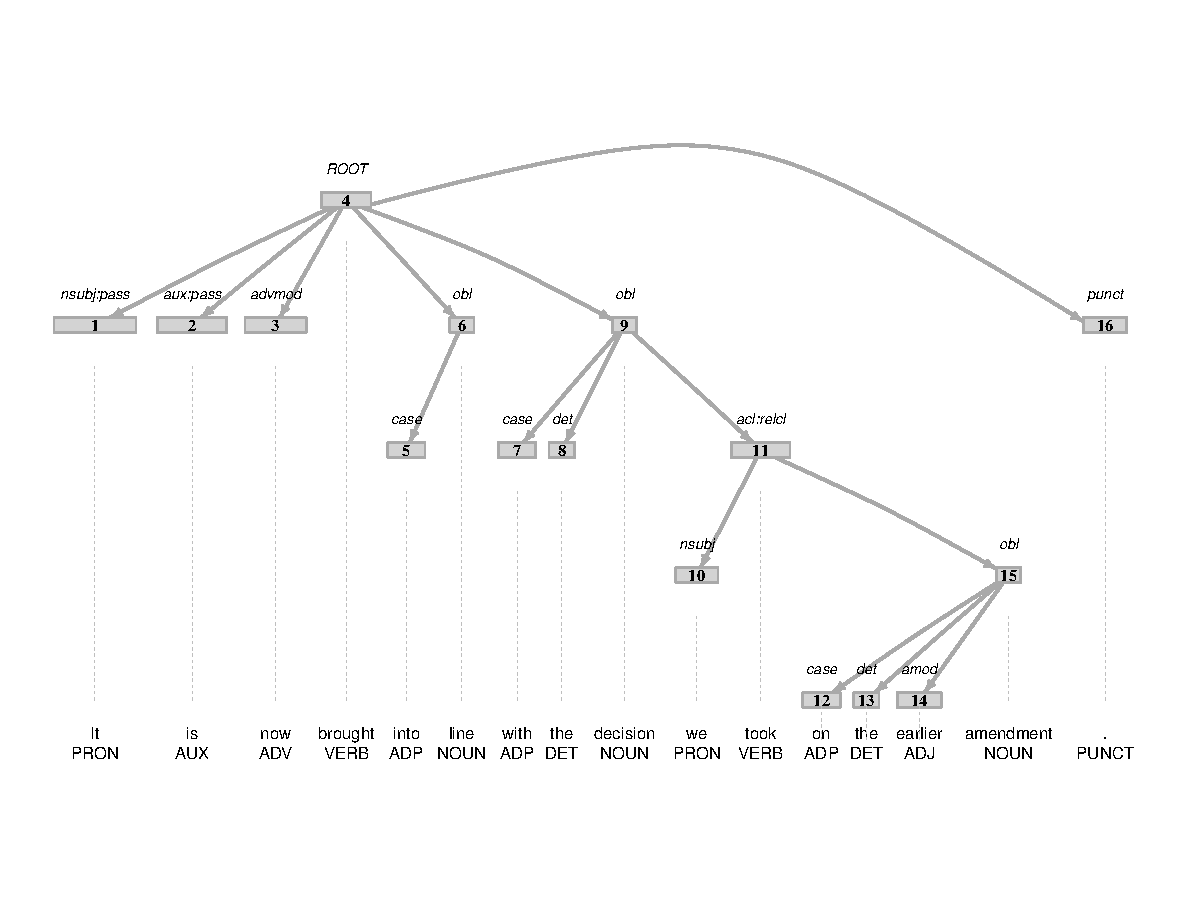
\includegraphics{part_3/7_transform_files/figure-pdf/fig-transform-generation-udpipe-english-plot-tree-1.pdf}

}

\caption{\label{fig-transform-generation-udpipe-english-plot-tree}Plot
of the syntactic tree for a sentence in the ENNTT natives dataset}

\end{figure}%

\begin{tcolorbox}[enhanced jigsaw, left=2mm, toprule=.15mm, colback=white, colframe=quarto-callout-color-frame, arc=.35mm, rightrule=.15mm, bottomrule=.15mm, leftrule=.75mm, breakable, opacityback=0]

\textbf{\faIcon{medal} Dive deeper}

The plot in
Figure~\ref{fig-transform-generation-udpipe-english-plot-tree} was
created using \{rsyntax\} (\citeproc{ref-R-rsyntax}{Welbers \& van
Atteveldt, 2022}). In addition to creating dependency tree plots,
\{rsyntax\} can be used to extract syntactic patterns from the
\texttt{udpipe()} annotation output.
\href{https://github.com/vanatteveldt/rsyntax}{See the documentation for
more information}.

\end{tcolorbox}

In Figure~\ref{fig-transform-generation-udpipe-english-plot-tree} we see
the syntactic tree for a sentence in the ENNTT natives dataset. Each
node is labeled with the \texttt{token\_id} which provides the linear
ordering of the sentence. Above the nodes the \texttt{dep\_relation}, or
dependency relationship label is provided. These labels are based on the
UD project's
\href{https://universaldependencies.org/u/dep/index.html}{dependency
relations}. We can see that the `ROOT' relation is at the top of the
tree and corresponds to the verb `brought'. `ROOT' relations mark
predicates in the sentence. Not seen in the example tree, `cop' relation
is a copular, or non-verbal predicate and should be included. These are
the key syntactic pattern we will use to identify main clauses for
T-units.

\subsection{Recoding}\label{sec-transform-recoding}

Recoding processes can be characterized by the creation of structural
changes which are derived from values in variables effectively recasting
values as new variables to enable more direct access in our analyses.

Specifically, we will need to identify and count the main clauses and
their subordinate clauses to create a variable \texttt{t\_units} from
our natives and translations annotations objects. In the UD project's
listings, the relations `ccomp' (clausal complement), `xcomp' (open
clausal complement), and `acl:relcl' (relative clause), as seen in
Figure~\ref{fig-transform-generation-udpipe-english-plot-tree} are
subordinate clauses. Furthermore, we will also need to count the number
of words in each sentence to create a variable \texttt{word\_len}.

To calculate T-units and words per sentence we turn to \{dplyr\}. We
will use the \texttt{group\_by()} function to group the dataset by
\texttt{doc\_id} and \texttt{sentence\_id} and then use the
\texttt{summarize()} function to calculate the number of T-units and
words per sentence, where a T-unit is the combination of the sum of main
clauses and sum of subordinante clauses. The code is seen in
Example~\ref{exm-transform-generation-udpipe-natives-tunits-words}.

\begin{example}[]\protect\hypertarget{exm-transform-generation-udpipe-natives-tunits-words}{}\label{exm-transform-generation-udpipe-natives-tunits-words}

~

\begin{Shaded}
\begin{Highlighting}[]
\CommentTok{\# Calculate the number of T{-}units and words per sentence}
\NormalTok{enntt\_natives\_syn\_comp\_tbl }\OtherTok{\textless{}{-}}
\NormalTok{  enntt\_natives\_ann\_tbl }\SpecialCharTok{|\textgreater{}}
  \FunctionTok{group\_by}\NormalTok{(doc\_id, sentence\_id) }\SpecialCharTok{|\textgreater{}}
  \FunctionTok{summarize}\NormalTok{(}
    \AttributeTok{main\_clauses =} \FunctionTok{sum}\NormalTok{(dep\_rel }\SpecialCharTok{\%in\%} \FunctionTok{c}\NormalTok{(}\StringTok{"ROOT"}\NormalTok{, }\StringTok{"cop"}\NormalTok{)),}
    \AttributeTok{subord\_clauses =} \FunctionTok{sum}\NormalTok{(dep\_rel }\SpecialCharTok{\%in\%} \FunctionTok{c}\NormalTok{(}\StringTok{"ccomp"}\NormalTok{, }\StringTok{"xcomp"}\NormalTok{, }\StringTok{"acl:relcl"}\NormalTok{)),}
    \AttributeTok{t\_units =}\NormalTok{ main\_clauses }\SpecialCharTok{+}\NormalTok{ subord\_clauses,}
    \AttributeTok{word\_len =} \FunctionTok{n}\NormalTok{()}
\NormalTok{  ) }\SpecialCharTok{|\textgreater{}}
  \FunctionTok{ungroup}\NormalTok{()}

\CommentTok{\# Preview}
\FunctionTok{glimpse}\NormalTok{(enntt\_natives\_syn\_comp\_tbl)}
\end{Highlighting}
\end{Shaded}

\begin{verbatim}
Rows: 10,199
Columns: 6
$ doc_id         <chr> "1", "10", "100", "1000", "10000", "1001", "1002", "100~
$ sentence_id    <int> 1, 1, 1, 1, 1, 1, 1, 1, 1, 1, 1, 1, 1, 1, 1, 1, 1, 1, 1~
$ main_clauses   <int> 1, 0, 0, 0, 2, 0, 0, 1, 1, 0, 1, 1, 1, 0, 2, 0, 1, 1, 1~
$ subord_clauses <int> 3, 2, 1, 0, 1, 2, 1, 1, 0, 2, 1, 0, 3, 2, 0, 4, 2, 1, 1~
$ t_units        <int> 4, 2, 1, 0, 3, 2, 1, 2, 1, 2, 2, 1, 4, 2, 2, 4, 3, 2, 2~
$ word_len       <int> 21, 25, 27, 15, 40, 43, 29, 23, 13, 30, 33, 9, 68, 35, ~
\end{verbatim}

\end{example}

A quick spot check of some sentences calculations
\texttt{enntt\_natives\_syn\_comp\_tbl} dataset against the
\texttt{enntt\_natives\_ann\_tbl} is good to ensure that the calculation
is working as expected. In
Figure~\ref{fig-transform-generation-udpipe-natives-tunits} we see a
sentence that has a word length of 13 and a T-unit value of 5.

\begin{figure}[!htb]

\centering{

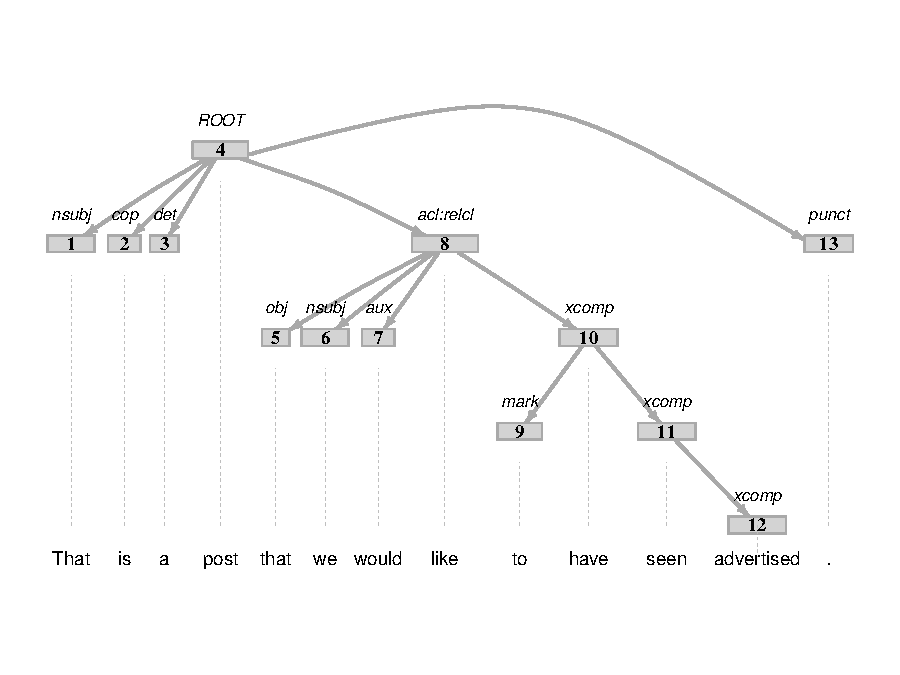
\includegraphics{part_3/7_transform_files/figure-pdf/fig-transform-generation-udpipe-natives-tunits-1.pdf}

}

\caption{\label{fig-transform-generation-udpipe-natives-tunits}Sentence
with a word length of 13 and a T-unit value of 5}

\end{figure}%

Now we can drop the intermediate columns we created to calculate our key
syntactic complexity measures using \texttt{select()} to indicate those
that we do want to keep, as seen in
Example~\ref{exm-transform-generation-udpipe-natives-tunits-words-select}.

\begin{example}[]\protect\hypertarget{exm-transform-generation-udpipe-natives-tunits-words-select}{}\label{exm-transform-generation-udpipe-natives-tunits-words-select}

~

\begin{Shaded}
\begin{Highlighting}[]
\CommentTok{\# Select columns}
\NormalTok{enntt\_natives\_syn\_comp\_tbl }\OtherTok{\textless{}{-}}
\NormalTok{  enntt\_natives\_syn\_comp\_tbl }\SpecialCharTok{|\textgreater{}}
  \FunctionTok{select}\NormalTok{(doc\_id, sentence\_id, t\_units, word\_len)}
\end{Highlighting}
\end{Shaded}

\end{example}

Now we can repeat the process for the ENNTT translated dataset. I will
assign the result to \texttt{enntt\_translations\_syn\_comp\_tbl}. The
next step is to join the \texttt{sentences} from the annotated data
frames into our datasets so that we have the information we set out to
generate for both datasets. Then we will combine the native and
translations datasets into a single dataset. These steps are part of the
transformation process and will be covered in the next section.

\subsection{Integration}\label{sec-transform-integration}

One final class of transformations that can be applied to curated
datasets to enhance their informativeness for a research project is the
process of integrating two or more datasets. There are two primary types
of integrations: joins and concatenation. \textbf{Joins} can be row- or
column-wise operations that combine datasets based on a common attribute
or set of attributes. \textbf{Concatenation} is exclusively a row-wise
operation that combines datasets that share the same attributes.

Of the two types, joins are the most powerful and sometimes more
difficult to understand. When two datasets are joined at least one
common variable must be shared between the two datasets. The common
variable(s) are referred to as \textbf{keys}. The keys are used to match
observations in one dataset with observations in another dataset by
serving as an index.

There are a number of join types. The most common are left, full, semi,
and anti. The type of join determines which observations are retained in
the resulting dataset. Let's see this in practice. First, let's create
two datasets to join with a common variable \texttt{key}, as seen in
Example~\ref{exm-transform-merging-join-dfs}.

\begin{example}[]\protect\hypertarget{exm-transform-merging-join-dfs}{}\label{exm-transform-merging-join-dfs}

~

\begin{Shaded}
\begin{Highlighting}[]
\NormalTok{a\_tbl }\OtherTok{\textless{}{-}}
  \FunctionTok{tibble}\NormalTok{(}
    \AttributeTok{key =} \FunctionTok{c}\NormalTok{(}\DecValTok{1}\NormalTok{, }\DecValTok{2}\NormalTok{, }\DecValTok{3}\NormalTok{, }\DecValTok{5}\NormalTok{, }\DecValTok{8}\NormalTok{),}
    \AttributeTok{a =}\NormalTok{ letters[}\DecValTok{1}\SpecialCharTok{:}\DecValTok{5}\NormalTok{]}
\NormalTok{  )}

\NormalTok{a\_tbl}
\NormalTok{b\_tbl }\OtherTok{\textless{}{-}}
  \FunctionTok{tibble}\NormalTok{(}
    \AttributeTok{key =} \FunctionTok{c}\NormalTok{(}\DecValTok{1}\NormalTok{, }\DecValTok{2}\NormalTok{, }\DecValTok{4}\NormalTok{, }\DecValTok{6}\NormalTok{, }\DecValTok{8}\NormalTok{),}
    \AttributeTok{b =}\NormalTok{ letters[}\DecValTok{6}\SpecialCharTok{:}\DecValTok{10}\NormalTok{]}
\NormalTok{  )}

\NormalTok{b\_tbl}
\end{Highlighting}
\end{Shaded}

\begin{figure}

\begin{minipage}{0.50\linewidth}

\begin{verbatim}
# A tibble: 5 x 2
    key a    
  <dbl> <chr>
1     1 a    
2     2 b    
3     3 c    
4     5 d    
5     8 e    
\end{verbatim}

\end{minipage}%
%
\begin{minipage}{0.50\linewidth}

\begin{verbatim}
# A tibble: 5 x 2
    key b    
  <dbl> <chr>
1     1 f    
2     2 g    
3     4 h    
4     6 i    
5     8 j    
\end{verbatim}

\end{minipage}%

\end{figure}%

\end{example}

The \texttt{a\_tbl} and the \texttt{b\_tbl} datasets share the
\texttt{key} variable, but the values in the \texttt{key} variable are
not identical. The two datasets share values \texttt{1}, \texttt{2}, and
\texttt{8}. The \texttt{a\_tbl} dataset has values \texttt{3} and
\texttt{5} in the \texttt{key} variable and the \texttt{b\_tbl} dataset
has values \texttt{4} and \texttt{6} in the \texttt{key} variable.

If we apply a left join to the \texttt{a\_tbl} and \texttt{b\_tbl}
datasets, the result will be a dataset that retains all of the
observations in the \texttt{a\_tbl} dataset and only those observations
in the \texttt{b\_tbl} dataset that have a match in the \texttt{a\_tbl}
dataset. The result is seen in
Example~\ref{exm-transform-merging-join-left}.

\begin{example}[]\protect\hypertarget{exm-transform-merging-join-left}{}\label{exm-transform-merging-join-left}

~

\begin{Shaded}
\begin{Highlighting}[]
\FunctionTok{left\_join}\NormalTok{(}\AttributeTok{x =}\NormalTok{ a\_tbl, }\AttributeTok{y =}\NormalTok{ b\_tbl, }\AttributeTok{by =} \StringTok{"key"}\NormalTok{)}
\end{Highlighting}
\end{Shaded}

\begin{verbatim}
# A tibble: 5 x 3
    key a     b    
  <dbl> <chr> <chr>
1     1 a     f    
2     2 b     g    
3     3 c     <NA> 
4     5 d     <NA> 
5     8 e     j    
\end{verbatim}

\end{example}

Now, if the key variable has the same name, R will recognize and assume
that this is the variable to join on and we don't need the
\texttt{by\ =} argument, but if there are multiple potential key
variables, we use \texttt{by\ =} to specify which one to use.

A full join retains all observations in both datasets, as seen in
Example~\ref{exm-transform-merging-join-full}.

\begin{example}[]\protect\hypertarget{exm-transform-merging-join-full}{}\label{exm-transform-merging-join-full}

~

\begin{Shaded}
\begin{Highlighting}[]
\FunctionTok{full\_join}\NormalTok{(}\AttributeTok{x =}\NormalTok{ a\_tbl, }\AttributeTok{y =}\NormalTok{ b\_tbl)}
\end{Highlighting}
\end{Shaded}

\begin{verbatim}
# A tibble: 7 x 3
    key a     b    
  <dbl> <chr> <chr>
1     1 a     f    
2     2 b     g    
3     3 c     <NA> 
4     5 d     <NA> 
5     8 e     j    
6     4 <NA>  h    
7     6 <NA>  i    
\end{verbatim}

\end{example}

Left and full joins maintain or increase the number of observations. On
the other hand, semi and anti joins aim to decrease the number of
observations. A semi join retains only those observations in the left
dataset that have a match in the right dataset, as seen in
Example~\ref{exm-transform-merging-join-semi}.

\begin{example}[]\protect\hypertarget{exm-transform-merging-join-semi}{}\label{exm-transform-merging-join-semi}

~

\begin{Shaded}
\begin{Highlighting}[]
\FunctionTok{semi\_join}\NormalTok{(}\AttributeTok{x =}\NormalTok{ a\_tbl, }\AttributeTok{y =}\NormalTok{ b\_tbl)}
\end{Highlighting}
\end{Shaded}

\begin{verbatim}
# A tibble: 3 x 2
    key a    
  <dbl> <chr>
1     1 a    
2     2 b    
3     8 e    
\end{verbatim}

\end{example}

And an anti join retains only those observations in the left dataset
that do not have a match in the right dataset, as seen in
Example~\ref{exm-transform-merging-join-anti}.

\begin{example}[]\protect\hypertarget{exm-transform-merging-join-anti}{}\label{exm-transform-merging-join-anti}

~

\begin{Shaded}
\begin{Highlighting}[]
\FunctionTok{anti\_join}\NormalTok{(}\AttributeTok{x =}\NormalTok{ a\_tbl, }\AttributeTok{y =}\NormalTok{ b\_tbl)}
\end{Highlighting}
\end{Shaded}

\begin{verbatim}
# A tibble: 2 x 2
    key a    
  <dbl> <chr>
1     3 c    
2     5 d    
\end{verbatim}

\end{example}

Of these join types, the left join and the anti join are some of the
most common to encounter in research projects.

\begin{tcolorbox}[enhanced jigsaw, left=2mm, toprule=.15mm, colback=white, colframe=quarto-callout-color-frame, arc=.35mm, rightrule=.15mm, bottomrule=.15mm, leftrule=.75mm, breakable, opacityback=0]

\textbf{\faIcon{lightbulb} Consider this}

In addition to datasets that are part of an acquired resource or derived
from a corpus resource, there are also a number of datasets that are
included in R packages that are particularly relevant for text analysis.
For example, \{tidytext\} includes \texttt{sentiments} and
\texttt{stop\_words} datasets. \{lexicon\}
(\citeproc{ref-R-lexicon}{Rinker, 2019}) includes large number of
datasets that include sentiment lexicons, stopword lists, contractions,
and more.

\end{tcolorbox}

With this in mind, let's return to our syntactic simplification
investigation. Recall that we started with two curated ENNTT datasets:
the natives and translations. We manipulated these datasets subsetting
them to 10,000 randomly selected lines, prepped them for annotation by
adding a \texttt{doc\_id} column and dropping all columns except
\texttt{text}, and then annotated them using \{udpipe\}. We then
calculated the number of T-units and words per sentence and created the
variables \texttt{t\_units} and \texttt{word\_len} for each.

These steps produced two datasets for both the natives and for the
translations. The first dataset for each is the annotated data frame.
The second is the data frame with the sytactic complexity measures we
calculated. The annotated data frames are named
\texttt{enntt\_natives\_ann\_tbl} and
\texttt{enntt\_translations\_ann\_tbl}. The data frames with the
syntactic complexity measures are named
\texttt{enntt\_natives\_syn\_comp\_tbl} and
\texttt{enntt\_translations\_syn\_comp\_tbl}.

In the end, we want a dataset that looks something like
Table~\ref{tbl-transform-integration-idealized}.

\begin{longtable}[]{@{}
  >{\raggedright\arraybackslash}p{(\columnwidth - 8\tabcolsep) * \real{0.1500}}
  >{\raggedright\arraybackslash}p{(\columnwidth - 8\tabcolsep) * \real{0.1500}}
  >{\raggedright\arraybackslash}p{(\columnwidth - 8\tabcolsep) * \real{0.1500}}
  >{\raggedright\arraybackslash}p{(\columnwidth - 8\tabcolsep) * \real{0.1500}}
  >{\raggedright\arraybackslash}p{(\columnwidth - 8\tabcolsep) * \real{0.4000}}@{}}
\caption{Idealized integrated dataset for the syntactic simplification
investigation}\label{tbl-transform-integration-idealized}\tabularnewline
\toprule\noalign{}
\begin{minipage}[b]{\linewidth}\raggedright
doc\_id
\end{minipage} & \begin{minipage}[b]{\linewidth}\raggedright
type
\end{minipage} & \begin{minipage}[b]{\linewidth}\raggedright
t\_units
\end{minipage} & \begin{minipage}[b]{\linewidth}\raggedright
word\_len
\end{minipage} & \begin{minipage}[b]{\linewidth}\raggedright
text
\end{minipage} \\
\midrule\noalign{}
\endfirsthead
\toprule\noalign{}
\begin{minipage}[b]{\linewidth}\raggedright
doc\_id
\end{minipage} & \begin{minipage}[b]{\linewidth}\raggedright
type
\end{minipage} & \begin{minipage}[b]{\linewidth}\raggedright
t\_units
\end{minipage} & \begin{minipage}[b]{\linewidth}\raggedright
word\_len
\end{minipage} & \begin{minipage}[b]{\linewidth}\raggedright
text
\end{minipage} \\
\midrule\noalign{}
\endhead
\bottomrule\noalign{}
\endlastfoot
1 & natives & 1 & 5 & I am happy right now. \\
2 & translation & 3 & 11 & I think that John believes that Mary is a
good person. \\
\end{longtable}

To create this unified dataset, we will need to apply joins and
concatenation. First, we will join the prepped datasets with the
annotated datasets. Then, we will concatenate the two resulting
datasets.

Let's start by joining the annotated datasets
(\texttt{enntt\_natives\_ann\_tbl} and
\texttt{enntt\_translations\_ann\_tbl}) with the datasets with the
syntactic complexity calculations
(\texttt{enntt\_natives\_syn\_comp\_tbl} and
\texttt{enntt\_translations\_syn\_comp\_tbl}). In these joins, we can
see that the prepped and calculated datasets share a couple variables,
\texttt{doc\_id} and \texttt{sentence\_id}, in
Example~\ref{exm-transform-merging-join-prepped-syn-comp}.

\begin{example}[]\protect\hypertarget{exm-transform-merging-join-prepped-syn-comp}{}\label{exm-transform-merging-join-prepped-syn-comp}

~

\begin{Shaded}
\begin{Highlighting}[]
\CommentTok{\# Preview datasets to join}
\NormalTok{enntt\_natives\_ann\_tbl }\SpecialCharTok{|\textgreater{}}
  \FunctionTok{slice\_head}\NormalTok{(}\AttributeTok{n =} \DecValTok{3}\NormalTok{)}
\end{Highlighting}
\end{Shaded}

\begin{verbatim}
# A tibble: 3 x 17
  doc_id paragraph_id sentence_id sentence    start   end term_id token_id token
  <chr>         <int>       <int> <chr>       <int> <int>   <int> <chr>    <chr>
1 1                 1           1 It is extr~     1     2       1 1        It   
2 1                 1           1 It is extr~     4     5       2 2        is   
3 1                 1           1 It is extr~     7    15       3 3        extr~
# i 8 more variables: lemma <chr>, upos <chr>, xpos <chr>, feats <chr>,
#   head_token_id <chr>, dep_rel <chr>, deps <chr>, misc <chr>
\end{verbatim}

\begin{Shaded}
\begin{Highlighting}[]
\NormalTok{enntt\_natives\_syn\_comp\_tbl }\SpecialCharTok{|\textgreater{}}
  \FunctionTok{slice\_head}\NormalTok{(}\AttributeTok{n =} \DecValTok{3}\NormalTok{)}
\end{Highlighting}
\end{Shaded}

\begin{verbatim}
# A tibble: 3 x 4
  doc_id sentence_id t_units word_len
  <chr>        <int>   <int>    <int>
1 1                1       4       21
2 10               1       2       25
3 100              1       1       27
\end{verbatim}

\end{example}

The \texttt{doc\_id} and \texttt{sentence\_id} variables are both keys
that we will use to join the datasets. The reason being that if we only
use one of the two we will not align the two datasets at the sentence
level. Only the combination of \texttt{doc\_id} and
\texttt{sentence\_id} isolates the sentences for which we have syntactic
complexity measures. Beyond a having common variable (or variables in
our case), we must also ensure that join key variables are of the same
vector type in both data frames and that we are aware of any differences
in the values. From the output in
Example~\ref{exm-transform-merging-join-prepped-syn-comp}, we can see
that the \texttt{doc\_id} and \texttt{sentence\_id} variables aligned in
terms of vector type; \texttt{doc\_id} is character and
\texttt{sentence\_id} is integer in both data frames. If they happened
not to be, their types would need to be adjusted.

Now, we need to check for differences in the values. We can do this by
using the \texttt{setequal()} function. This function returns
\texttt{TRUE} if the two vectors are equal and \texttt{FALSE} if they
are not. If the two vectors are not equal, the function will return the
values that are in one vector but not the other. So if one has
\texttt{10001} and the other doesn't we will get \texttt{FALSE}. Let's
see this in practice, as seen in
Example~\ref{exm-transform-merging-join-prepped-syn-comp-check}.

\begin{example}[]\protect\hypertarget{exm-transform-merging-join-prepped-syn-comp-check}{}\label{exm-transform-merging-join-prepped-syn-comp-check}

~

\begin{Shaded}
\begin{Highlighting}[]
\CommentTok{\# Check for differences in the values}
\FunctionTok{setequal}\NormalTok{(}
\NormalTok{  enntt\_natives\_ann\_tbl}\SpecialCharTok{$}\NormalTok{doc\_id,}
\NormalTok{  enntt\_natives\_syn\_comp\_tbl}\SpecialCharTok{$}\NormalTok{doc\_id}
\NormalTok{)}
\end{Highlighting}
\end{Shaded}

\begin{verbatim}
[1] TRUE
\end{verbatim}

\begin{Shaded}
\begin{Highlighting}[]
\FunctionTok{setequal}\NormalTok{(}
\NormalTok{  enntt\_natives\_ann\_tbl}\SpecialCharTok{$}\NormalTok{sentence\_id,}
\NormalTok{  enntt\_natives\_syn\_comp\_tbl}\SpecialCharTok{$}\NormalTok{sentence\_id}
\NormalTok{)}
\end{Highlighting}
\end{Shaded}

\begin{verbatim}
[1] TRUE
\end{verbatim}

\end{example}

So the values are the same. The final check is to see if the vectors are
of the same length. We know the values are the same, but we don't know
if the values are repeated. We do this by simply comparing the length of
the vectors, as seen in
Example~\ref{exm-transform-merging-join-prepped-syn-comp-length}.

\begin{example}[]\protect\hypertarget{exm-transform-merging-join-prepped-syn-comp-length}{}\label{exm-transform-merging-join-prepped-syn-comp-length}

~

\begin{Shaded}
\begin{Highlighting}[]
\CommentTok{\# Check for differences in the length}
\FunctionTok{length}\NormalTok{(enntt\_natives\_ann\_tbl}\SpecialCharTok{$}\NormalTok{doc\_id) }\SpecialCharTok{==}
  \FunctionTok{length}\NormalTok{(enntt\_natives\_syn\_comp\_tbl}\SpecialCharTok{$}\NormalTok{doc\_id)}
\end{Highlighting}
\end{Shaded}

\begin{verbatim}
[1] FALSE
\end{verbatim}

\begin{Shaded}
\begin{Highlighting}[]
\FunctionTok{length}\NormalTok{(enntt\_natives\_ann\_tbl}\SpecialCharTok{$}\NormalTok{sentence\_id) }\SpecialCharTok{==}
  \FunctionTok{length}\NormalTok{(enntt\_natives\_syn\_comp\_tbl}\SpecialCharTok{$}\NormalTok{sentence\_id)}
\end{Highlighting}
\end{Shaded}

\begin{verbatim}
[1] FALSE
\end{verbatim}

\end{example}

So they are not the same length. Using the \texttt{nrow()} function, I
can see that the annotated dataset has 264,124 observations and the
calculated dataset has 10,199 observations. The annotation data frames
will have many more observations due to the fact that the unit of
observations is word tokens. The recoded syntactic complexity data
frames' unit of observation is the sentence.

To appreciate the difference in the number of observations, let's look
at the first 10 observations of the natives annotated frame for just the
columns of interest, as seen in
Example~\ref{exm-transform-merging-join-prepped-syn-comp-ann}.

\begin{example}[]\protect\hypertarget{exm-transform-merging-join-prepped-syn-comp-ann}{}\label{exm-transform-merging-join-prepped-syn-comp-ann}

~

\begin{Shaded}
\begin{Highlighting}[]
\CommentTok{\# Preview the annotated dataset}
\NormalTok{enntt\_natives\_ann\_tbl }\SpecialCharTok{|\textgreater{}}
  \FunctionTok{select}\NormalTok{(doc\_id, sentence\_id, sentence, token) }\SpecialCharTok{|\textgreater{}}
  \FunctionTok{slice\_head}\NormalTok{(}\AttributeTok{n =} \DecValTok{10}\NormalTok{)}
\end{Highlighting}
\end{Shaded}

\begin{verbatim}
# A tibble: 10 x 4
   doc_id sentence_id sentence                                             token
   <chr>        <int> <chr>                                                <chr>
 1 1                1 It is extremely important that action is taken to e~ It   
 2 1                1 It is extremely important that action is taken to e~ is   
 3 1                1 It is extremely important that action is taken to e~ extr~
 4 1                1 It is extremely important that action is taken to e~ impo~
 5 1                1 It is extremely important that action is taken to e~ that 
 6 1                1 It is extremely important that action is taken to e~ acti~
 7 1                1 It is extremely important that action is taken to e~ is   
 8 1                1 It is extremely important that action is taken to e~ taken
 9 1                1 It is extremely important that action is taken to e~ to   
10 1                1 It is extremely important that action is taken to e~ ensu~
\end{verbatim}

\end{example}

The annotated data frames have a lot of redundancy in for the join
variables and the \texttt{sentence} variable that we want to add to the
calculated data frames. We can reduce the redundancy by using the
\texttt{distinct()} function from \{dplyr\}. In this case we want all
observations where \texttt{doc\_id}, \texttt{sentence\_id} and
\texttt{sentence} are distinct. We then select these variables with
\texttt{distinct()}, as seen in
Example~\ref{exm-transform-merging-annotation-distinct}.

\begin{example}[]\protect\hypertarget{exm-transform-merging-annotation-distinct}{}\label{exm-transform-merging-annotation-distinct}

~

\begin{Shaded}
\begin{Highlighting}[]
\CommentTok{\# Reduce annotated data frames to unique sentences}
\NormalTok{enntt\_natives\_ann\_distinct }\OtherTok{\textless{}{-}}
\NormalTok{  enntt\_natives\_ann\_tbl }\SpecialCharTok{|\textgreater{}}
  \FunctionTok{distinct}\NormalTok{(doc\_id, sentence\_id, sentence)}

\NormalTok{enntt\_translations\_ann\_distinct }\OtherTok{\textless{}{-}}
\NormalTok{  enntt\_translations\_ann\_tbl }\SpecialCharTok{|\textgreater{}}
  \FunctionTok{distinct}\NormalTok{(doc\_id, sentence\_id, sentence)}
\end{Highlighting}
\end{Shaded}

\end{example}

We now have two datasets that are ready to be joined with the recoded
datasets. The next step is to join the two. We will employ a left join
where the syntactic complexity data frames are on the left and the join
variables will be both the \texttt{doc\_id} and \texttt{sentence\_id}
variables. The code is seen in
Example~\ref{exm-transform-merging-join-left-syn-comp}.

\begin{example}[]\protect\hypertarget{exm-transform-merging-join-left-syn-comp}{}\label{exm-transform-merging-join-left-syn-comp}

~

\begin{Shaded}
\begin{Highlighting}[]
\CommentTok{\# Join the native datasets}
\NormalTok{enntt\_natives\_transformed\_tbl }\OtherTok{\textless{}{-}}
  \FunctionTok{left\_join}\NormalTok{(}
    \AttributeTok{x =}\NormalTok{ enntt\_natives\_syn\_comp\_tbl,}
    \AttributeTok{y =}\NormalTok{ enntt\_natives\_ann\_distinct,}
    \AttributeTok{by =} \FunctionTok{c}\NormalTok{(}\StringTok{"doc\_id"}\NormalTok{, }\StringTok{"sentence\_id"}\NormalTok{)}
\NormalTok{  )}

\CommentTok{\# Preview}
\FunctionTok{glimpse}\NormalTok{(enntt\_natives\_transformed\_tbl)}
\end{Highlighting}
\end{Shaded}

\begin{verbatim}
Rows: 10,199
Columns: 5
$ doc_id      <chr> "1", "10", "100", "1000", "10000", "1001", "1002", "1003",~
$ sentence_id <int> 1, 1, 1, 1, 1, 1, 1, 1, 1, 1, 1, 1, 1, 1, 1, 1, 1, 1, 1, 1~
$ t_units     <int> 4, 2, 1, 0, 3, 2, 1, 2, 1, 2, 2, 1, 4, 2, 2, 4, 3, 2, 2, 1~
$ word_len    <int> 21, 25, 27, 15, 40, 43, 29, 23, 13, 30, 33, 9, 68, 35, 16,~
$ sentence    <chr> "It is extremely important that action is taken to ensure ~
\end{verbatim}

\begin{Shaded}
\begin{Highlighting}[]
\CommentTok{\# Join the translations datasets}
\NormalTok{enntt\_translations\_transformed\_tbl }\OtherTok{\textless{}{-}}
  \FunctionTok{left\_join}\NormalTok{(}
    \AttributeTok{x =}\NormalTok{ enntt\_translations\_syn\_comp\_tbl,}
    \AttributeTok{y =}\NormalTok{ enntt\_translations\_ann\_distinct,}
    \AttributeTok{by =} \FunctionTok{c}\NormalTok{(}\StringTok{"doc\_id"}\NormalTok{, }\StringTok{"sentence\_id"}\NormalTok{)}
\NormalTok{  )}

\CommentTok{\# Preview}
\FunctionTok{glimpse}\NormalTok{(enntt\_translations\_transformed\_tbl)}
\end{Highlighting}
\end{Shaded}

\begin{verbatim}
Rows: 10,392
Columns: 5
$ doc_id      <chr> "1", "10", "100", "1000", "10000", "1001", "1002", "1003",~
$ sentence_id <int> 1, 1, 1, 1, 1, 1, 1, 1, 1, 1, 1, 1, 1, 1, 1, 1, 1, 1, 1, 1~
$ t_units     <int> 0, 2, 0, 1, 3, 0, 3, 2, 3, 3, 2, 0, 1, 0, 3, 1, 0, 1, 2, 2~
$ word_len    <int> 24, 31, 5, 39, 44, 26, 67, 23, 46, 28, 24, 68, 19, 18, 36,~
$ sentence    <chr> "To my great surprise , on leaving the sitting , I found t~
\end{verbatim}

\end{example}

The two data frames now have the same columns and we are closer to our
final dataset. The next step is to move toward concatenating the two
datasets. Before we do that, we need to do some preparation. First, and
most important, we need to add a \texttt{type} column to each dataset.
This column will indicate whether the sentence is a native or a
translation. The second is that our \texttt{doc\_id} does not serve as a
unique identifier for the sentences. Only in combination with
\texttt{sentence\_id} can we uniquely identify a sentence.

So our plan will be to add a \texttt{type} column to each dataset
specifying the values for all the observations in the respective
dataset. Then we will concatenate the two datasets. Note, if we combine
them before, distiguishing the type will be more difficult. After we
concatenate the two datasets, we will add a \texttt{doc\_id} column that
will serve as a unique identifier for the sentences and drop the
\texttt{sentence\_id} column. OK, that's the plan. Let's execute it in
Example~\ref{exm-transform-merging-concatenation}.

\begin{example}[]\protect\hypertarget{exm-transform-merging-concatenation}{}\label{exm-transform-merging-concatenation}

~

\begin{Shaded}
\begin{Highlighting}[]
\CommentTok{\# Add a type column}
\NormalTok{enntt\_natives\_transformed\_tbl }\OtherTok{\textless{}{-}}
\NormalTok{  enntt\_natives\_transformed\_tbl }\SpecialCharTok{|\textgreater{}}
  \FunctionTok{mutate}\NormalTok{(}\AttributeTok{type =} \StringTok{"natives"}\NormalTok{)}

\NormalTok{enntt\_translations\_transformed\_tbl }\OtherTok{\textless{}{-}}
\NormalTok{  enntt\_translations\_transformed\_tbl }\SpecialCharTok{|\textgreater{}}
  \FunctionTok{mutate}\NormalTok{(}\AttributeTok{type =} \StringTok{"translations"}\NormalTok{)}

\CommentTok{\# Concatenate the datasets}
\NormalTok{enntt\_transformed\_tbl }\OtherTok{\textless{}{-}}
  \FunctionTok{bind\_rows}\NormalTok{(}
\NormalTok{    enntt\_natives\_transformed\_tbl,}
\NormalTok{    enntt\_translations\_transformed\_tbl}
\NormalTok{  )}

\CommentTok{\# Overwrite the doc\_id column with a unique identifier}
\NormalTok{enntt\_transformed\_tbl }\OtherTok{\textless{}{-}}
\NormalTok{  enntt\_transformed\_tbl }\SpecialCharTok{|\textgreater{}}
  \FunctionTok{mutate}\NormalTok{(}\AttributeTok{doc\_id =} \FunctionTok{row\_number}\NormalTok{()) }\SpecialCharTok{|\textgreater{}}
  \FunctionTok{select}\NormalTok{(doc\_id, type, t\_units, word\_len, }\AttributeTok{text =}\NormalTok{ sentence)}

\CommentTok{\# Preview}
\FunctionTok{glimpse}\NormalTok{(enntt\_transformed\_tbl)}
\end{Highlighting}
\end{Shaded}

\begin{verbatim}
Rows: 20,591
Columns: 5
$ doc_id   <int> 1, 2, 3, 4, 5, 6, 7, 8, 9, 10, 11, 12, 13, 14, 15, 16, 17, 18~
$ type     <chr> "natives", "natives", "natives", "natives", "natives", "nativ~
$ t_units  <int> 4, 2, 1, 0, 3, 2, 1, 2, 1, 2, 2, 1, 4, 2, 2, 4, 3, 2, 2, 1, 1~
$ word_len <int> 21, 25, 27, 15, 40, 43, 29, 23, 13, 30, 33, 9, 68, 35, 16, 53~
$ text     <chr> "It is extremely important that action is taken to ensure tha~
\end{verbatim}

\end{example}

The output of Example~\ref{exm-transform-merging-concatenation} now
looks like Table~\ref{tbl-transform-integration-idealized}. We have a
dataset that has the syntactic complexity measures for both the natives
and the translations. We can now write this dataset to disk and document
it in the data dictionary.

\section*{Activities}\label{activities-5}
\addcontentsline{toc}{section}{Activities}

\markright{Activities}

In the following activities, you will review the concept of transforming
data to prepare it for analysis and working to implement these steps
with R. This includes preparation and enrichment of curated datasets
using normalization, tokenization, recoding, generation, and/ or
integration strategies.

\begin{tcolorbox}[enhanced jigsaw, left=2mm, toprule=.15mm, colback=white, colframe=quarto-callout-color-frame, arc=.35mm, rightrule=.15mm, bottomrule=.15mm, leftrule=.75mm, breakable, opacityback=0]

\textbf{\faIcon{file-code} Recipe}

\textbf{What}: Transforming and documenting datasets\\
\textbf{How}: Read Recipe 7, complete comprehension check, and prepare
for Lab 7.\\
\textbf{Why}: To work with to primary types of transformations,
tokenization and joins. Tokenization is the process of recasting textual
units as smaller textual units. The process of joining datasets aims to
incorporate other datasets to augment or filter the dataset of interest.

\end{tcolorbox}

\begin{tcolorbox}[enhanced jigsaw, left=2mm, toprule=.15mm, colback=white, colframe=quarto-callout-color-frame, arc=.35mm, rightrule=.15mm, bottomrule=.15mm, leftrule=.75mm, breakable, opacityback=0]

\textbf{\faIcon{flask} Lab}

\textbf{What}: Dataset alchemy\\
\textbf{How}: Fork, clone, and complete the steps in Lab 7.\\
\textbf{Why}: To gain experience working with coding strategies for
transforming datasets using tidyverse functions and regexes, practice
reading/ writing data from/ to disk, and implement organizational
strategies for organizing and documenting a dataset in reproducible
fashion.

\end{tcolorbox}

\section*{Summary}\label{summary-6}
\addcontentsline{toc}{section}{Summary}

\markright{Summary}

In this chapter we covered the process of transforming datasets. The
goal is to manipulate the curated dataset to make it align better for
analysis. We covered various types of transformation procedures from
text normalization to data frame integrations. In any given research
project some or all of these steps will be employed --but not
necessarily in the order presented in this chapter. It is not uncommon
to mix procedures as well. The etiology of the transformation is as
unique as the data that you are working with.

Since you are applying techniques that have a significant factor on the
shape and contents of your dataset(s) it is important to perform data
checks to ensure that the transformations are working as expected. You
may not catch everything, and some things may not be caught until later
in the analysis process, but it is important to do as much as you can as
early as you can.

In line with the reproducible research principles, it is important to
write the transformed dataset to disk and to document it in the data
dictionary. This is especially important if you are working with
multiple datasets. Good naming conventions also come into play. Choosing
descriptive names is so easily overlooked by your present self but so
welcomed by your future self.

\part{Analysis}

In this part, we turn to the analysis of datasets, the evaluation of
results, and the interpretation of the findings. We will outline the
three main types of statistical analyses: Exploratory Data Analysis
(EDA), Predictive Data Analysis (PDA), and Inferential Data Analysis
(IDA). Each of these analysis types have distinct, non-overlapping aims
and therefore should be determined from the outset of the research
project and included as part of the research blueprint. The aim of this
section is to establish a clearer picture of the goals, methods, and
value of each of these approaches.

\chapter{Explore}\label{sec-explore-chapter}

\begin{quote}
The data speaks for itself, but only if we are willing to listen.

--- Nate Silver
\end{quote}

\begin{tcolorbox}[enhanced jigsaw, left=2mm, toprule=.15mm, colback=white, colframe=quarto-callout-color-frame, arc=.35mm, rightrule=.15mm, bottomrule=.15mm, leftrule=.75mm, breakable, opacityback=0]

\textbf{\faIcon{list-alt} Outcomes}

\begin{itemize}
\tightlist
\item
  Determine the suitability of exploratory data analysis for a research
  project.
\item
  Understand descriptive analysis and unsupervised learning methods,
  their strengths in pattern recognition and data summarization.
\item
  Interpret insights from data summarization and pattern recognition,
  considering their potential to guide further research.
\end{itemize}

\end{tcolorbox}

In this chapter, we examine a wide range of strategies for exploratory
data analysis. The chapter outlines two main branches of exploratory
data analysis: descriptive analysis which statistically and/ or visually
summarizes a dataset and unsupervised learning which is a machine
learning approach that does not assume any particular relationship
between variables in a dataset. Either through descriptive or
unsupervised learning methods, exploratory data analysis employs
quantitative methods to summarize, reduce, and sort complex datasets and
statistically and visually interrogate a dataset in order to provide the
researcher novel perspective to be qualitatively assessed.

\begin{tcolorbox}[enhanced jigsaw, left=2mm, toprule=.15mm, colback=white, colframe=quarto-callout-color-frame, arc=.35mm, rightrule=.15mm, bottomrule=.15mm, leftrule=.75mm, breakable, opacityback=0]

\textbf{\faIcon{terminal} Lessons}

\textbf{What}: Advanced objects\\
\textbf{How}: In an R console, load \{swirl\}, run \texttt{swirl()}, and
follow prompts to select the lesson.\\
\textbf{Why}: To learn about advanced objects in R, including lists and
matrices, and create, inspect, access, and manipulate these objects.

\end{tcolorbox}

\section{Orientation}\label{sec-explore-orientation}

The goal of exploratory data analysis is to discover, describe, and
posit new hypotheses. This analysis approach is best-suited for research
questions where the literature scarce, where the gap in knowledge is
wide, or where new territories are being explored. The researcher may
not know what to expect, but they are willing to let the data speak for
itself. The researcher is open to new insights and new questions that
may emerge from the analysis process.

While exploratory data analysis allows flexibility, it is essential to
have a guiding research question that provides a focus for the analysis.
This question will help to determine the variables of interest and the
methods to be used. The research question will also help to determine
the relevance of the results and the potential for the results to be
used in further research.

The general workflow for exploratory data analysis is shown in
Table~\ref{tbl-explore-workflow}.

\begin{longtable}[]{@{}
  >{\centering\arraybackslash}p{(\columnwidth - 4\tabcolsep) * \real{0.0500}}
  >{\raggedright\arraybackslash}p{(\columnwidth - 4\tabcolsep) * \real{0.1500}}
  >{\raggedright\arraybackslash}p{(\columnwidth - 4\tabcolsep) * \real{0.8000}}@{}}
\caption{Workflow for exploratory data
analysis}\label{tbl-explore-workflow}\tabularnewline
\toprule\noalign{}
\begin{minipage}[b]{\linewidth}\centering
Step
\end{minipage} & \begin{minipage}[b]{\linewidth}\raggedright
Name
\end{minipage} & \begin{minipage}[b]{\linewidth}\raggedright
Description
\end{minipage} \\
\midrule\noalign{}
\endfirsthead
\toprule\noalign{}
\begin{minipage}[b]{\linewidth}\centering
Step
\end{minipage} & \begin{minipage}[b]{\linewidth}\raggedright
Name
\end{minipage} & \begin{minipage}[b]{\linewidth}\raggedright
Description
\end{minipage} \\
\midrule\noalign{}
\endhead
\bottomrule\noalign{}
\endlastfoot
1 & Identify & Consider the research question and identify variables of
potential interest to provide insight into our question. \\
2 & Inspect & Check for missing data, outliers, \emph{etc}. and check
data distributions and transform if necessary. \\
3 & Interrogate & Submit the selected variables to descriptive
(frequency, keyword, co-occurrence analysis, \emph{etc.}) or
unsupervised learning (clustering, dimensionality reduction, vector
spacing modeling, \emph{etc.}) methods to provide quantitative measures
to evaluate. \\
4 & Interpret & Evaluate the results and determine if they are valid and
meaningful to respond to the research question. \\
5 & Iterate (Optional) & Repeat steps 1-4 as new questions emerge from
your interpretation. \\
\end{longtable}

\section{Analysis}\label{sec-explore-analysis}

To frame our demonstration and discussion of exploratory data analysis,
let's tackle a task. The task will be to identify relevant materials for
an English Language Learner (ELL) textbook. This will involve multiple
research questions and allow us to illustrate some very fundamental
concepts that emerge across text analysis research in both descriptive
and unsupervised learning approaches.

Since our task is geared towards English language use, we will want a
representative data sample. For this, we will use the Manually Annotated
Sub-Corpus (MASC) of the American National Corpus
(\citeproc{ref-Ide2008}{Ide et al., 2008}).

The data dictionary for the dataset we will use as our point of
departure is shown in Table~\ref{tbl-explore-masc-dd-show}.

\begin{longtable}[]{@{}
  >{\raggedright\arraybackslash}p{(\columnwidth - 6\tabcolsep) * \real{0.1500}}
  >{\raggedright\arraybackslash}p{(\columnwidth - 6\tabcolsep) * \real{0.1500}}
  >{\raggedright\arraybackslash}p{(\columnwidth - 6\tabcolsep) * \real{0.1500}}
  >{\raggedright\arraybackslash}p{(\columnwidth - 6\tabcolsep) * \real{0.5500}}@{}}

\caption{\label{tbl-explore-masc-dd-show}Data dictionary for the MASC
dataset.}

\tabularnewline

\toprule\noalign{}
\begin{minipage}[b]{\linewidth}\raggedright
variable
\end{minipage} & \begin{minipage}[b]{\linewidth}\raggedright
name
\end{minipage} & \begin{minipage}[b]{\linewidth}\raggedright
type
\end{minipage} & \begin{minipage}[b]{\linewidth}\raggedright
description
\end{minipage} \\
\midrule\noalign{}
\endhead
\bottomrule\noalign{}
\endlastfoot
doc\_id & Document ID & numeric & Unique identifier for each document \\
modality & Modality & categorical & The form in which the document is
presented (written or spoken) \\
genre & Genre & categorical & The category or type of the document \\
term\_num & Term Number & numeric & Index number term per document \\
term & Term & categorical & Individual word forms in the document \\
lemma & Lemma & categorical & Base or dictionary form of the term \\
pos & Part of Speech & categorical & Grammatical category of the term
(modified PENN Treebank tagset) \\

\end{longtable}

First, I'll read in and preview the dataset in
Example~\ref{exm-explore-masc-read}.

\begin{example}[]\protect\hypertarget{exm-explore-masc-read}{}\label{exm-explore-masc-read}

~

\begin{Shaded}
\begin{Highlighting}[]
\CommentTok{\# Read the dataset}
\NormalTok{masc\_tbl }\OtherTok{\textless{}{-}}
  \FunctionTok{read\_csv}\NormalTok{(}\StringTok{"../data/masc/masc\_transformed.csv"}\NormalTok{)}

\CommentTok{\# Preview the MASC dataset}
\NormalTok{masc\_tbl }\SpecialCharTok{|\textgreater{}} \FunctionTok{glimpse}\NormalTok{()}
\end{Highlighting}
\end{Shaded}

\begin{verbatim}
Rows: 591,036
Columns: 7
$ doc_id   <dbl> 1, 1, 1, 1, 1, 1, 1, 1, 1, 1, 1, 1, 1, 1, 1, 1, 1, 1, 1, 1, 1~
$ modality <chr> "Written", "Written", "Written", "Written", "Written", "Writt~
$ genre    <chr> "Letters", "Letters", "Letters", "Letters", "Letters", "Lette~
$ term_num <dbl> 0, 1, 2, 3, 4, 5, 6, 7, 8, 9, 10, 11, 12, 13, 14, 15, 16, 17,~
$ term     <chr> "December", "1998", "Your", "contribution", "to", "Goodwill",~
$ lemma    <chr> "december", "1998", "your", "contribution", "to", "goodwill",~
$ pos      <chr> "NNP", "CD", "PRP$", "NN", "TO", "NNP", "MD", "VB", "JJR", "I~
\end{verbatim}

\end{example}

From the output in Example~\ref{exm-explore-masc-read}, we get some
sense of the structure of the dataset. However, we also need to perform
diagnostic and descriptive procedures. This will include checking for
missing data and anomalies and assessing central tendency, dispersion,
and/ or distributions of the variables. This may include using
\{skimr\}, \{dplyr\}, \{stringr\}, \{ggplot2\}, \emph{etc.} to identify
the most relevant variables for our task and to identify any potential
issues with the dataset.

After a descriptive and diagnostic assessment of the dataset, not
included here, I identified and addressed missing data and anomalies
(including many non-words). I also recoded the \texttt{doc\_id} variable
to a character variable. The dataset now has 486,368 observations, a
reduction from the original 591,036 observations. There are 392
documents, 2 modalities, 18 genres, almost 38k unique terms (which are
words), almost 26k lemmas (word base forms), and 34 distinct part of
speech (POS) tags.

\subsection{Descriptive analysis}\label{sec-explore-descriptive}

Descriptive analysis includes common techniques such as frequency
analysis to determine the most frequent words or phrases, dispersion
analysis to see how terms are distributed throughout a document or
corpus, keyword analysis to identify distinctive terms, and/ or
co-occurrence analysis to see what terms tend to appear together.

Using the MASC dataset, we will entertain questions such as:

\begin{itemize}
\tightlist
\item
  What are the most common terms a beginning ELL should learn?
\item
  Are there term differences between spoken and written discourses that
  should be emphasized?
\item
  What are some of the most common verb particle constructions?
\end{itemize}

Along the way, we will introduce touch on frequency, dispersion, and
co-occurrence measures. In addition, we will apply various descriptive
analysis techniques and visualizations to explore the dataset and
identify new questions and new variables of interest.

\subsubsection{Frequency analysis}\label{sec-explore-frequency}

At its core, frequency analysis is a descriptive method that counts the
number of times a linguistic unit occurs in a dataset. The results of
frequency analysis can be used to describe the dataset and to identify
terms that are linguistically distinctive or distinctive to a particular
group or sub-group in the dataset.

\paragraph{Raw frequency}\label{sec-explore-frequency-raw}

Let's consider what the most common words in the MASC dataset are as a
starting point to making inroads on our task by identifying relevant
vocabulary for an ELL textbook.

In the \texttt{masc\_tbl} data frame we have the linguistic unit
\texttt{term} which corresponds to the word-level annotation of the
MASC. The \texttt{lemma} corresponds to the base form of each term, for
words with inflectional morphology, the lemma is the word sans the
inflection (\emph{e.g.} is - be, are - be). For other words, the
\texttt{term} and the \texttt{lemma} will be the same (\emph{e.g.} the -
the, in - in). These two variables pose a choice point for us: do we
consider words to be the actual forms or the base forms? There is an
argument to be made for both. In this case, I will operationalize our
linguistic unit as the \texttt{lemma} variable, as this will allow us to
group words with distinct inflectional morphology together.

To perform a basic word frequency analysis, we can apply
\texttt{summarize()} in combination with \texttt{n()} or the convenient
\texttt{count()} function from \{dplyr\}. Our sorted lemma counts appear
in Example~\ref{exm-explore-masc-count}.

\begin{example}[]\protect\hypertarget{exm-explore-masc-count}{}\label{exm-explore-masc-count}

~

\begin{Shaded}
\begin{Highlighting}[]
\CommentTok{\# Lemma count, sorted in descending order}
\NormalTok{masc\_tbl }\SpecialCharTok{|\textgreater{}}
  \FunctionTok{count}\NormalTok{(lemma, }\AttributeTok{sort =} \ConstantTok{TRUE}\NormalTok{)}
\end{Highlighting}
\end{Shaded}

\begin{verbatim}
# A tibble: 25,923 x 2
   lemma     n
   <chr> <int>
 1 the   26137
 2 be    19466
 3 to    13548
 4 and   12528
 5 of    12005
 6 a     10461
 7 in     8374
 8 i      7783
 9 that   7082
10 you    5276
# i 25,913 more rows
\end{verbatim}

\end{example}

The output of this frequency tabulation in
Example~\ref{exm-explore-masc-count} is a data frame with two columns:
\texttt{lemma} and \texttt{n}.

As we discussed in Section~\ref{sec-analysis-distributions}, the
frequency of linguistic units in a corpus tends to be highly
right-skewed distribution, approximating the Zipf distribution. If we
calculate the \textbf{cumulative frequency}, a rolling sum of the
frequency term by term, of the lemmas in the \texttt{masc\_tbl} data
frame, we can see that the top 10 types account for around 25\% of the
lemmas used in the entire corpus --by 100 types that increases to near
50\% and 1,000 around 75\%, as seen in
Example~\ref{exm-explore-masc-count-cumulative}.

\begin{example}[]\protect\hypertarget{exm-explore-masc-count-cumulative}{}\label{exm-explore-masc-count-cumulative}

~

\begin{figure}[!htb]

\centering{

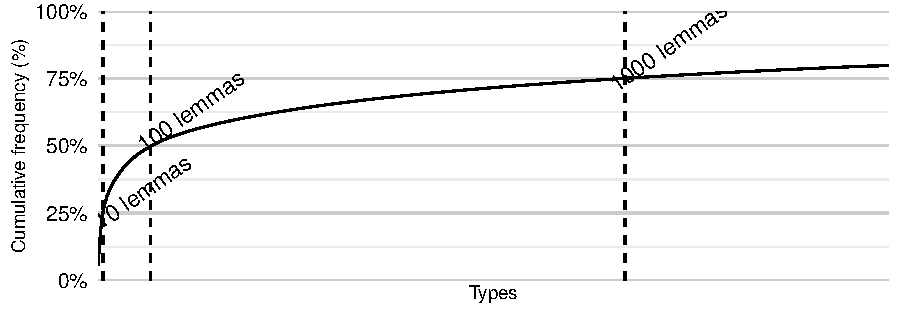
\includegraphics{part_4/8_explore_files/figure-pdf/fig-explore-masc-count-cumulative-1.pdf}

}

\caption{\label{fig-explore-masc-count-cumulative}Cumulative frequency
of lemmas in the MASC dataset}

\end{figure}%

\end{example}

If we look at the types that appear within the first 50 most frequent,
you can likely also appreciate another thing about language use. Let's
list the top 50 types in Example~\ref{exm-explore-masc-count-top-50}.

\begin{example}[]\protect\hypertarget{exm-explore-masc-count-top-50}{}\label{exm-explore-masc-count-top-50}

~

\begin{Shaded}
\begin{Highlighting}[]
\CommentTok{\# Top 50 types}
\NormalTok{lemma\_cumul\_freq }\SpecialCharTok{|\textgreater{}}
  \FunctionTok{slice\_head}\NormalTok{(}\AttributeTok{n =} \DecValTok{50}\NormalTok{) }\SpecialCharTok{|\textgreater{}}
  \FunctionTok{pull}\NormalTok{(lemma) }\SpecialCharTok{|\textgreater{}}
  \FunctionTok{matrix}\NormalTok{(}\AttributeTok{ncol =} \DecValTok{5}\NormalTok{) }\SpecialCharTok{|\textgreater{}}
  \FunctionTok{kable}\NormalTok{(}\AttributeTok{col.names =} \ConstantTok{NULL}\NormalTok{)}
\end{Highlighting}
\end{Shaded}

\begin{longtable}[]{@{}
  >{\raggedright\arraybackslash}p{(\columnwidth - 8\tabcolsep) * \real{0.2000}}
  >{\raggedright\arraybackslash}p{(\columnwidth - 8\tabcolsep) * \real{0.2000}}
  >{\raggedright\arraybackslash}p{(\columnwidth - 8\tabcolsep) * \real{0.2000}}
  >{\raggedright\arraybackslash}p{(\columnwidth - 8\tabcolsep) * \real{0.2000}}
  >{\raggedright\arraybackslash}p{(\columnwidth - 8\tabcolsep) * \real{0.2000}}@{}}

\caption{\label{tbl-explore-masc-count-top-50}Top 50 lemma types in the
MASC dataset.}

\tabularnewline

\toprule\noalign{}
\endhead
\bottomrule\noalign{}
\endlastfoot
the & have & at & your & all \\
be & it & from & an & there \\
to & for & he & say & me \\
and & on & but & what & would \\
of & do & by & so & about \\
a & with & will & his & know \\
in & we & my & if & get \\
i & as & or & 's & make \\
that & this & n't & can & out \\
you & not & they & go & up \\

\end{longtable}

\end{example}

For the most part, the most frequent words are not content words, but
rather function words (\emph{e.g.} determiners, prepositions, pronouns,
auxiliary verbs). Function words include a closed class of relatively
few words that are used to express grammatical relationships between
content words. It then is no surprise that they are the comprise many of
the most frequent words in a corpus.

Another key observation is that among the most frequency content words
(\emph{e.g.} nouns, verbs, adjectives, adverbs) are words that are quite
semantically generic --that is, they are words that are used in a wide
range of contexts and take a wide range of meanings.

Take for example the adjective `good'. It can be used to describe a wide
range of nouns, such as `good food', `good people', `good times',
\emph{etc}. A sometimes near-synonym of `good', for example `good
student', is the word `studious'. Yet, `studious' is not as frequent as
`good' as it is used to describe a narrower range of nouns, such as
`studious student', `studious scholar', `studious researcher',
\emph{etc}. In this way, `studious' is more semantically specific than
`good'.

\begin{tcolorbox}[enhanced jigsaw, left=2mm, toprule=.15mm, colback=white, colframe=quarto-callout-color-frame, arc=.35mm, rightrule=.15mm, bottomrule=.15mm, leftrule=.75mm, breakable, opacityback=0]

\textbf{\faIcon{lightbulb} Consider this}

Based on what you now know about the expected distribution of words in a
corpus, what if your were asked to predict what the most frequency
English word used is in each U.S. State? What would you predict? How
confident would you be in your prediction? What if you were asked to
predict what the most frequency word used is in the language of a given
country? What would you want to know before making your prediction?

\end{tcolorbox}

So common across corpus samples, in some analyses these usual suspects
of the most common words are considered irrelvant and are filtered out.
In our ELL materials task, however, we might exclude them for this
simple fact that it will be a given that we will teach these words given
their grammatical importance. If we want to focus on the most common
content words, we can filter out the function words.

One approach to filtering out these words is to use a pre-determined
list of \textbf{stopwords}. \{tidytext\} includes a data frame
\texttt{stop\_words} of stopword lexicons for English. We can select a
lexicon from \texttt{stop\_words} and use \texttt{anti\_join()} to
filter out the words that appear in the \texttt{word} variable from the
\texttt{lemma} variable in the \texttt{masc\_tbl} data frame.

Eliminating words in this fashion, however, may not always be the best
approach. Available lists of stopwords vary in their contents and are
determined by other researchers for other potential uses. We may instead
opt to create our own stopword list that is tailored to the task, or we
may opt to use a statistical approach based on their distribution in the
dataset using frequency and/ or dispersion measures.

For our case, however, we have another available strategy. Since our
task is to identify relevant vocabulary, beyond the fundamental function
words in English, we can use the POS tags to reduce our dataset to just
the content words, that is nouns, verbs, adjectives, and adverbs.

We need to consult the Penn Tagset again, to ensure we are selecting the
correct tags. I will assign this data frame to
\texttt{masc\_content\_tbl} to keep it separate from our main data frame
\texttt{masc\_tbl}, seen in Example~\ref{exm-explore-masc-filter-pos}.

\begin{example}[]\protect\hypertarget{exm-explore-masc-filter-pos}{}\label{exm-explore-masc-filter-pos}

~

\begin{Shaded}
\begin{Highlighting}[]
\CommentTok{\# Penn Tagset for content words}
\CommentTok{\# Nouns: NN, NNS,}
\CommentTok{\# Verbs: VB, VBD, VBG, VBN, VBP, VBZ}
\CommentTok{\# Adjectives: JJ, JJR, JJS}
\CommentTok{\# Adverbs: RB, RBR, RBS}

\NormalTok{content\_pos }\OtherTok{\textless{}{-}} \FunctionTok{c}\NormalTok{(}\StringTok{"NN"}\NormalTok{, }\StringTok{"NNS"}\NormalTok{, }\StringTok{"VB"}\NormalTok{, }\StringTok{"VBD"}\NormalTok{, }\StringTok{"VBG"}\NormalTok{, }\StringTok{"VBN"}\NormalTok{, }\StringTok{"VBP"}\NormalTok{, }\StringTok{"VBZ"}\NormalTok{, }\StringTok{"JJ"}\NormalTok{, }\StringTok{"JJR"}\NormalTok{, }\StringTok{"JJS"}\NormalTok{, }\StringTok{"RB"}\NormalTok{, }\StringTok{"RBR"}\NormalTok{, }\StringTok{"RBS"}\NormalTok{)}

\CommentTok{\# Select content words}
\NormalTok{masc\_content\_tbl }\OtherTok{\textless{}{-}}
\NormalTok{  masc\_tbl }\SpecialCharTok{|\textgreater{}}
  \FunctionTok{filter}\NormalTok{(pos }\SpecialCharTok{\%in\%}\NormalTok{ content\_pos)}

\CommentTok{\# Preview top 50}
\NormalTok{masc\_content\_tbl }\SpecialCharTok{|\textgreater{}}
  \FunctionTok{count}\NormalTok{(lemma, }\AttributeTok{sort =} \ConstantTok{TRUE}\NormalTok{) }\SpecialCharTok{|\textgreater{}}
  \FunctionTok{slice\_head}\NormalTok{(}\AttributeTok{n =} \DecValTok{50}\NormalTok{) }\SpecialCharTok{|\textgreater{}}
  \FunctionTok{pull}\NormalTok{(lemma) }\SpecialCharTok{|\textgreater{}}
  \FunctionTok{matrix}\NormalTok{(}\AttributeTok{ncol =} \DecValTok{5}\NormalTok{) }\SpecialCharTok{|\textgreater{}}
  \FunctionTok{kable}\NormalTok{(}\AttributeTok{col.names =} \ConstantTok{NULL}\NormalTok{)}
\end{Highlighting}
\end{Shaded}

\begin{longtable}[]{@{}
  >{\raggedright\arraybackslash}p{(\columnwidth - 8\tabcolsep) * \real{0.2000}}
  >{\raggedright\arraybackslash}p{(\columnwidth - 8\tabcolsep) * \real{0.2000}}
  >{\raggedright\arraybackslash}p{(\columnwidth - 8\tabcolsep) * \real{0.2000}}
  >{\raggedright\arraybackslash}p{(\columnwidth - 8\tabcolsep) * \real{0.2000}}
  >{\raggedright\arraybackslash}p{(\columnwidth - 8\tabcolsep) * \real{0.2000}}@{}}

\caption{\label{tbl-explore-masc-filter-pos}Frequency of tokens in the
MASC dataset after filtering out lemmas with POS tags that are not
content words}

\tabularnewline

\toprule\noalign{}
\endhead
\bottomrule\noalign{}
\endlastfoot
be & think & work & also & t \\
have & more & year & need & first \\
do & just & come & way & help \\
not & time & use & back & day \\
n't & so & well & here & many \\
say & other & look & new & man \\
go & see & then & find & ask \\
know & people & right & give & very \\
get & take & only & thing & much \\
make & now & want & tell & even \\

\end{longtable}

\end{example}

The resulting list in Table~\ref{tbl-explore-masc-filter-pos} paints a
different picture of the most frequent words in the dataset. The most
frequent words are now content words, and included in most frequent
words are more semantically specific words. We now have reduced the
number of observations by 50\% focusing on the content words. We are
getting closer to identifying the vocabulary that we want to include in
our ELL materials, but we will need some more tools to help us identify
the most relevant vocabulary.

\paragraph{Dispersion}\label{sec-explore-frequency-dispersion}

\textbf{Dispersion} is a measure of how evenly distributed a linguistic
unit is across a dataset. This is a key concept in text analysis, as
important as frequency. It is important to recognize that frequency and
dispersion are measures of different characteristics. We can have two
words that occur with the same frequency, but one word may be more
evenly distributed across a dataset than the other. Depending on the
researcher's aims, this may be an important distinction to make. For our
task, it is likely the case that we want to capture words that are
well-dispersed across the dataset as words that have a high frequency
and a low dispersion tend to be connected to a particular context,
whether that be a particular genre, a particular speaker, a particular
topic, \emph{etc}. In other research, aim may be the reverse; to
identify words that are highly frequent and highly concentrated in a
particular context to identify words that are distinctive to that
context.

There are a variety of measures that can be used to estimate the
distribution of types across a corpus. Let's focus on three measures:
document frequency (\(df\)), inverse document frequency (\(idf\)), and
Gries' Deviation of Proportions (\(dp\)).

The most basic measure is \textbf{document frequency} (\(df\)). This is
the number of documents in which a type appears at least once. For
example, if a type appears in 10 documents, then the document frequency
is 10. This is a very basic measure, but it is a good starting point.

A nuanced version of document frequency is \textbf{inverse document
frequency} (\(idf\)). This measure takes the total number of documents
and divides it by the document frequency. This results in a measure that
is inversely proportional to the document frequency. That is, the higher
the document frequency, the lower the inverse document frequency. This
measure is often log-transformed to spread out the values.

One thing to consider about \(df\) and \(idf\) is that niether takes
into account the length of the documents in which the type appears nor
the spread of the type within each document. To take these factors into
account, we can use Gries' \textbf{Deviation of Proportions} (\(dp\))
measure (\citeproc{ref-Gries2023}{S. T. Gries, 2023, pp. 87--88}). The
\(dp\) measure considers the proportion of a type's frequency in each
document relative to its total frequency. This produces a measure that
is more sensitive to the distribution of a type within and across
documents in a corpus.

Let's consider how these measures differ with three scenarios:

Imagine a type with a token frequency of 100 appears in each of the 10
documents in a corpus.

A. Each of the documents is 100 words long. The type appears 10 times in
each document.\\
B. Each of the documents is 100 words long. But now the type appears
once in 9 documents and 91 times in 1 document.\\
C. Nine of the documents constitute 99\% of the corpus. The type appears
once in each of the 9 documents and 91 times in the 10th document.

Scenario A is the most dispersed, scenario B is less dispersed, and
scenario C is the least dispersed. Yet, the type's \(df\) and \(idf\)
scores will be the same. But the \(dp\) score will reflect increasing
concentration of the type's dispersion from A to B to C.

\begin{tcolorbox}[enhanced jigsaw, left=2mm, toprule=.15mm, colback=white, colframe=quarto-callout-color-frame, arc=.35mm, rightrule=.15mm, bottomrule=.15mm, leftrule=.75mm, breakable, opacityback=0]

\textbf{\faIcon{medal} Dive deeper} Dispersion measures

You may wonder why we would want to use \(df\) or \(idf\) at all. The
answer is some combination of the fact that they are computationally
less expensive to calculate, they are widely used (especially \(idf\)),
and/ or in many practical situations they often highly correlated with
\(dp\).

\end{tcolorbox}

So for our task we will use \(dp\) as our measure of dispersion.
\{qtkit\} includes the \texttt{calc\_type\_metrics()} function which
calculates, among other metrics, the dispersion metrics \(df\), \(idf\),
and/ or \(dp\). Let's select \texttt{dp} and assign the result to
\texttt{masc\_lemma\_disp}, as seen in
Example~\ref{exm-explore-masc-dp}.

\begin{example}[]\protect\hypertarget{exm-explore-masc-dp}{}\label{exm-explore-masc-dp}

~

\begin{Shaded}
\begin{Highlighting}[]
\CommentTok{\# Load package}
\FunctionTok{library}\NormalTok{(qtkit)}

\CommentTok{\# Calculate deviance of proportions (DP)}
\NormalTok{masc\_lemma\_disp }\OtherTok{\textless{}{-}}
\NormalTok{  masc\_content\_tbl }\SpecialCharTok{|\textgreater{}}
  \FunctionTok{calc\_type\_metrics}\NormalTok{(}
    \AttributeTok{type =}\NormalTok{ lemma,}
    \AttributeTok{documents =}\NormalTok{ doc\_id,}
    \AttributeTok{dispersion =} \StringTok{"dp"}
\NormalTok{  ) }\SpecialCharTok{|\textgreater{}}
  \FunctionTok{arrange}\NormalTok{(dp)}

\CommentTok{\# Preview}
\NormalTok{masc\_lemma\_disp }\SpecialCharTok{|\textgreater{}}
  \FunctionTok{slice\_head}\NormalTok{(}\AttributeTok{n =} \DecValTok{10}\NormalTok{)}
\end{Highlighting}
\end{Shaded}

\begin{verbatim}
# A tibble: 10 x 3
   type      n    dp
   <chr> <dbl> <dbl>
 1 be    19231 0.123
 2 have   5136 0.189
 3 not    2279 0.240
 4 make   1149 0.266
 5 other   882 0.269
 6 more   1005 0.276
 7 take    769 0.286
 8 only    627 0.286
 9 time    931 0.314
10 see     865 0.327
\end{verbatim}

\end{example}

We would like to identify lemmas that are frequent and well-dispersed.
But an important question arises, what is the threshold for frequency
and dispersion that we should use to identify the lemmas that we want to
include in our ELL materials?

There are statistical approaches to identifying natural breakpoints,
including clustering, but a visual inspection is often good enough for
practical purposes. Let's create a density plot to see if there is a
natural break in the distribution of our dispersion measure, as seen in
Figure~\ref{fig-explore-masc-dp-density}.

\begin{example}[]\protect\hypertarget{exm-explore-masc-dp-density}{}\label{exm-explore-masc-dp-density}

~

\begin{Shaded}
\begin{Highlighting}[]
\CommentTok{\# Density plot of dp}
\NormalTok{masc\_lemma\_disp }\SpecialCharTok{|\textgreater{}}
  \FunctionTok{ggplot}\NormalTok{(}\FunctionTok{aes}\NormalTok{(}\AttributeTok{x =}\NormalTok{ dp)) }\SpecialCharTok{+}
  \FunctionTok{geom\_density}\NormalTok{() }\SpecialCharTok{+}
  \FunctionTok{scale\_x\_continuous}\NormalTok{(}\AttributeTok{breaks =} \FunctionTok{seq}\NormalTok{(}\DecValTok{0}\NormalTok{, }\DecValTok{1}\NormalTok{, .}\DecValTok{1}\NormalTok{)) }\SpecialCharTok{+}
  \FunctionTok{labs}\NormalTok{(}\AttributeTok{x =} \StringTok{"Deviation of Proportions"}\NormalTok{)}
\end{Highlighting}
\end{Shaded}

\begin{figure}[!htb]

\centering{

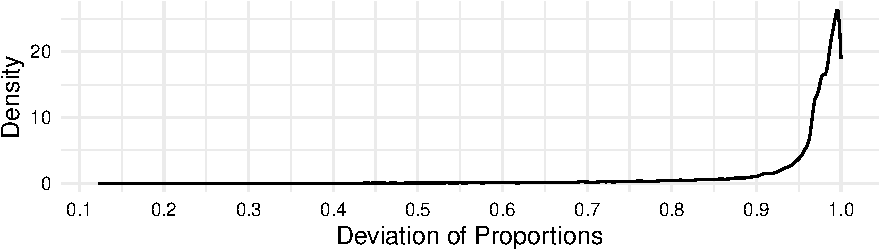
\includegraphics{part_4/8_explore_files/figure-pdf/fig-explore-masc-dp-density-1.pdf}

}

\caption{\label{fig-explore-masc-dp-density}Density plot of Deviation of
Proportions for lemmas in the MASC dataset}

\end{figure}%

\end{example}

What we are looking for is a distinctive bend in the distribution of
dispersion measures. In Figure~\ref{fig-explore-masc-dp-density}, we can
see one between 0.85 and 0.97. This bend is called an elbow, and using
this approach to make informed decisions about thresholds is called the
\textbf{elbow method}. We can split the difference and use this as a
threshold to filter out lemmas that are less dispersed.

In Example~\ref{exm-explore-masc-dp-filter}, I filter out lemmas that
have a dispersion measure less than 0.91.

\begin{example}[]\protect\hypertarget{exm-explore-masc-dp-filter}{}\label{exm-explore-masc-dp-filter}

~

\begin{Shaded}
\begin{Highlighting}[]
\CommentTok{\# Filter for lemmas with dp \textless{}= 0.91}
\NormalTok{masc\_lemma\_disp\_thr }\OtherTok{\textless{}{-}}
\NormalTok{  masc\_lemma\_disp }\SpecialCharTok{|\textgreater{}}
  \FunctionTok{filter}\NormalTok{(dp }\SpecialCharTok{\textless{}=} \FloatTok{0.91}\NormalTok{) }\SpecialCharTok{|\textgreater{}}
  \FunctionTok{arrange}\NormalTok{(}\FunctionTok{desc}\NormalTok{(n))}
\end{Highlighting}
\end{Shaded}

\end{example}

Then in Table~\ref{tbl-explore-masc-dp-filter-preview}, I preview the
top and bottom 50 lemmas in the dataset.

\begin{Shaded}
\begin{Highlighting}[]
\CommentTok{\# Preview top}
\NormalTok{masc\_lemma\_disp\_thr }\SpecialCharTok{|\textgreater{}}
  \FunctionTok{slice\_head}\NormalTok{(}\AttributeTok{n =} \DecValTok{50}\NormalTok{) }\SpecialCharTok{|\textgreater{}}
  \FunctionTok{pull}\NormalTok{(type) }\SpecialCharTok{|\textgreater{}}
  \FunctionTok{matrix}\NormalTok{(}\AttributeTok{ncol =} \DecValTok{5}\NormalTok{) }\SpecialCharTok{|\textgreater{}}
  \FunctionTok{kable}\NormalTok{(}\AttributeTok{col.names =} \ConstantTok{NULL}\NormalTok{)}
\CommentTok{\# Preview bottom}
\NormalTok{masc\_lemma\_disp\_thr }\SpecialCharTok{|\textgreater{}}
  \FunctionTok{slice\_tail}\NormalTok{(}\AttributeTok{n =} \DecValTok{50}\NormalTok{) }\SpecialCharTok{|\textgreater{}}
  \FunctionTok{pull}\NormalTok{(type) }\SpecialCharTok{|\textgreater{}}
  \FunctionTok{matrix}\NormalTok{(}\AttributeTok{ncol =} \DecValTok{5}\NormalTok{) }\SpecialCharTok{|\textgreater{}}
  \FunctionTok{kable}\NormalTok{(}\AttributeTok{col.names =} \ConstantTok{NULL}\NormalTok{)}
\end{Highlighting}
\end{Shaded}

\begin{table}

\caption{\label{tbl-explore-masc-dp-filter-preview}Frequency of tokens
in the MASC dataset after our dispersion threshold}

\begin{minipage}{\linewidth}

\subcaption{\label{tbl-explore-masc-dp-filter-preview-1}Top 50 lemmas}

\centering{

\begin{tabular}{lllll}
\toprule
be & think & work & also & t\\
have & more & year & way & first\\
do & just & come & need & help\\
not & time & use & back & day\\
n't & so & well & here & many\\
say & other & look & new & man\\
go & see & then & find & ask\\
know & people & right & give & very\\
get & take & only & thing & much\\
make & now & want & tell & even\\
\bottomrule
\end{tabular}

}

\end{minipage}%
\newline
\begin{minipage}{\linewidth}

\subcaption{\label{tbl-explore-masc-dp-filter-preview-2}Bottom 50 lemmas}

\centering{

\begin{tabular}{lllll}
\toprule
dump & tuition & blur & wound & accidentally\\
instrument & awaken & litigation & devote & protective\\
triumph & hook & resistance & alright & preside\\
harsh & fetch & absurd & evolutionary & rethink\\
ignorance & brave & qualify & envy & strictly\\
sting & unleash & liberty & nostalgic & wax\\
mainstream & prosperous & going & shy & faith-based\\
wildly & buzz & awkward & proximity & decidedly\\
dismiss & presume & afterwards & sandy & resolute\\
liability & summarize & eve & interfere & evidently\\
\bottomrule
\end{tabular}

}

\end{minipage}%

\end{table}%

We now have a good candidate list of common vocabulary that is spread
well across the corpus.

\paragraph{Relative frequency}\label{sec-explore-frequency-relative}

Gauging frequency and dispersion across the entire corpus is a good
starting point for any frequency analysis, but it is often the case that
we want to compare the frequency and dispersion of linguistic units
across corpora or sub-corpora.

In the case of the MASC dataset, for example, we may want to compare
metrics across the two modalities or the various genres. Simply
comparing frequency counts across these sub-corpora is not a good
approach, and can be misleading, as the sub-corpora may vary in size.
For example, if one sub-corpus is twice as large as another sub-corpus,
then, all else being equal, the frequency counts will be twice as large
in the larger sub-corpus. This is why we use relative frequency
measures, which are normalized by the size of the sub-corpus.

\begin{tcolorbox}[enhanced jigsaw, left=2mm, toprule=.15mm, colback=white, colframe=quarto-callout-color-frame, arc=.35mm, rightrule=.15mm, bottomrule=.15mm, leftrule=.75mm, breakable, opacityback=0]

\textbf{\faIcon{lightbulb} Consider this}

A variable in the MASC dataset that has yet to be used is the
\texttt{pos} POS variable. How could we use this variable to refine our
frequency and dispersion analysis of lemma types?

Hint: consider lemma forms that may be tagged with different
parts-of-speech.

\end{tcolorbox}

To normalize the frequency of linguistic units across sub-corpora, we
can use the \textbf{relative frequency} (\(rf\)) measure. This is the
frequency of a linguistic unit divided by the total number of linguistic
units in the sub-corpus. This bakes in the size of the sub-corpus into
the measure. The notion of relative frequency is key to all research
working with text, as it is the basis for the statistical approach to
text analysis where comparisons are made.

There are some field-specific terms that are used to refer to relative
frequency measures. For example, in information retrieval and Natural
Language Processing, the relative frequency measure is often referred to
as the \textbf{term frequency} (\(tf\)). In corpus linguistics, the
relative frequency measure is often modified slightly to include a
constant (\emph{e.g.} \(rf * 100\)) which is known as the
\textbf{observed relative frequency} (\(orf\)). Athough the observed
relative frequency per number of tokens is not strictly necessary, it is
often used to make the values more interpretable as we can now talk
about an observed relative frequency of 1.5 as a linguistic unit that
occurs 1.5 times per 100 linguistic units.

Let's consider how we might compare the frequency and dispersion of
lemmas across the two modalities in the MASC dataset, spoken and
written. To make this a bit more interesting and more relevant, let's
add the \texttt{pos} variable to our analysis. The intent, then, will be
to identify lemmas tagged with particular parts of speech that are
particularly indicative of each of the modaliites.

We can do this by collapsing the \texttt{lemma} and \texttt{pos}
variables into a single variable, \texttt{lemma\_pos}, with the
\texttt{str\_c()} function, as seen in
Example~\ref{exm-explore-masc-type}.

\begin{example}[]\protect\hypertarget{exm-explore-masc-type}{}\label{exm-explore-masc-type}

~

\begin{Shaded}
\begin{Highlighting}[]
\CommentTok{\# Collapse lemma and pos into type}
\NormalTok{masc\_content\_tbl }\OtherTok{\textless{}{-}}
\NormalTok{  masc\_content\_tbl }\SpecialCharTok{|\textgreater{}}
  \FunctionTok{mutate}\NormalTok{(}\AttributeTok{lemma\_pos =} \FunctionTok{str\_c}\NormalTok{(lemma, pos, }\AttributeTok{sep =} \StringTok{"\_"}\NormalTok{))}

\CommentTok{\# Preview}
\NormalTok{masc\_content\_tbl }\SpecialCharTok{|\textgreater{}}
  \FunctionTok{slice\_head}\NormalTok{(}\AttributeTok{n =} \DecValTok{5}\NormalTok{)}
\end{Highlighting}
\end{Shaded}

\begin{verbatim}
# A tibble: 5 x 8
  doc_id modality genre   term_num term         lemma        pos   lemma_pos    
  <chr>  <chr>    <chr>      <dbl> <chr>        <chr>        <chr> <chr>        
1 1      Written  Letters        3 contribution contribution NN    contribution~
2 1      Written  Letters        7 mean         mean         VB    mean_VB      
3 1      Written  Letters        8 more         more         JJR   more_JJR     
4 1      Written  Letters       12 know         know         VB    know_VB      
5 1      Written  Letters       15 help         help         VB    help_VB      
\end{verbatim}

\end{example}

Now this will increase the number of lemma types in the dataset as we
are now considering lemmas where the same lemma form is tagged with
different parts-of-speech.

Getting back to calculating the frequency and dispersion of lemmas in
each modality, we can use the \texttt{calc\_type\_metrics()} function
with \texttt{lemma\_pos} as our type argument. We will, however, need to
apply this function to each sub-corpus independently and then
concatenate the two data frames. This function returns a (raw) frequency
(\(n\)) measure by default, but we can specify the\texttt{frequency}
argument to \texttt{rf} to calculate the relative frequency of the
linguistic units as in Example~\ref{exm-explore-masc-metrics-modality}.

\begin{example}[]\protect\hypertarget{exm-explore-masc-metrics-modality}{}\label{exm-explore-masc-metrics-modality}

~

\begin{Shaded}
\begin{Highlighting}[]
\CommentTok{\# Calculate relative frequency}
\CommentTok{\# Spoken}
\NormalTok{masc\_spoken\_metrics }\OtherTok{\textless{}{-}}
\NormalTok{  masc\_content\_tbl }\SpecialCharTok{|\textgreater{}}
  \FunctionTok{filter}\NormalTok{(modality }\SpecialCharTok{==} \StringTok{"Spoken"}\NormalTok{) }\SpecialCharTok{|\textgreater{}}
  \FunctionTok{calc\_type\_metrics}\NormalTok{(}
    \AttributeTok{type =}\NormalTok{ lemma\_pos,}
    \AttributeTok{documents =}\NormalTok{ doc\_id,}
    \AttributeTok{frequency =} \StringTok{"rf"}\NormalTok{,}
    \AttributeTok{dispersion =} \StringTok{"dp"}
\NormalTok{  ) }\SpecialCharTok{|\textgreater{}}
  \FunctionTok{mutate}\NormalTok{(}\AttributeTok{modality =} \StringTok{"Spoken"}\NormalTok{) }\SpecialCharTok{|\textgreater{}}
  \FunctionTok{arrange}\NormalTok{(}\FunctionTok{desc}\NormalTok{(n))}

\CommentTok{\# Written}
\NormalTok{masc\_written\_metrics }\OtherTok{\textless{}{-}}
\NormalTok{  masc\_content\_tbl }\SpecialCharTok{|\textgreater{}}
  \FunctionTok{filter}\NormalTok{(modality }\SpecialCharTok{==} \StringTok{"Written"}\NormalTok{) }\SpecialCharTok{|\textgreater{}}
  \FunctionTok{calc\_type\_metrics}\NormalTok{(}
    \AttributeTok{type =}\NormalTok{ lemma\_pos,}
    \AttributeTok{documents =}\NormalTok{ doc\_id,}
    \AttributeTok{frequency =} \StringTok{"rf"}\NormalTok{,}
    \AttributeTok{dispersion =} \StringTok{"dp"}
\NormalTok{  ) }\SpecialCharTok{|\textgreater{}}
  \FunctionTok{mutate}\NormalTok{(}\AttributeTok{modality =} \StringTok{"Written"}\NormalTok{) }\SpecialCharTok{|\textgreater{}}
  \FunctionTok{arrange}\NormalTok{(}\FunctionTok{desc}\NormalTok{(n))}

\CommentTok{\# Concatenate spoken and written metrics}
\NormalTok{masc\_metrics }\OtherTok{\textless{}{-}}
  \FunctionTok{bind\_rows}\NormalTok{(masc\_spoken\_metrics, masc\_written\_metrics)}

\CommentTok{\# Preview}
\NormalTok{masc\_metrics }\SpecialCharTok{|\textgreater{}}
  \FunctionTok{slice\_head}\NormalTok{(}\AttributeTok{n =} \DecValTok{5}\NormalTok{)}
\end{Highlighting}
\end{Shaded}

\begin{verbatim}
# A tibble: 5 x 5
  type         n     rf     dp modality
  <chr>    <dbl>  <dbl>  <dbl> <chr>   
1 be_VBZ    2612 0.0489 0.0843 Spoken  
2 be_VBP    1282 0.0240 0.111  Spoken  
3 be_VBD    1020 0.0191 0.300  Spoken  
4 n't_RB     829 0.0155 0.139  Spoken  
5 have_VBP   766 0.0143 0.152  Spoken  
\end{verbatim}

\end{example}

With the \texttt{rf} measure, we are now in a position to compare
`apples to apples', as you might say. We can now compare the relative
frequency of lemmas across the two modalities. Let's preview the top 5
lemmas in each modality, as seen in
Example~\ref{exm-explore-masc-relative-frequency-top}.

\begin{example}[]\protect\hypertarget{exm-explore-masc-relative-frequency-top}{}\label{exm-explore-masc-relative-frequency-top}

~

\begin{Shaded}
\begin{Highlighting}[]
\CommentTok{\# Preview top 10 lemmas in each modality}
\NormalTok{masc\_metrics }\SpecialCharTok{|\textgreater{}}
  \FunctionTok{group\_by}\NormalTok{(modality) }\SpecialCharTok{|\textgreater{}}
  \FunctionTok{slice\_max}\NormalTok{(}\AttributeTok{n =} \DecValTok{10}\NormalTok{, }\AttributeTok{order\_by =}\NormalTok{ rf) }\SpecialCharTok{|\textgreater{}}
  \FunctionTok{ungroup}\NormalTok{()}
\end{Highlighting}
\end{Shaded}

\begin{verbatim}
# A tibble: 20 x 5
   type         n      rf     dp modality
   <chr>    <dbl>   <dbl>  <dbl> <chr>   
 1 be_VBZ    2612 0.0489  0.0843 Spoken  
 2 be_VBP    1282 0.0240  0.111  Spoken  
 3 be_VBD    1020 0.0191  0.300  Spoken  
 4 n't_RB     829 0.0155  0.139  Spoken  
 5 have_VBP   766 0.0143  0.152  Spoken  
 6 do_VBP     728 0.0136  0.180  Spoken  
 7 be_VB      655 0.0123  0.147  Spoken  
 8 not_RB     638 0.0119  0.137  Spoken  
 9 just_RB    404 0.00757 0.267  Spoken  
10 so_RB      387 0.00725 0.357  Spoken  
11 be_VBZ    4745 0.0249  0.230  Written 
12 be_VBD    3317 0.0174  0.366  Written 
13 be_VBP    2617 0.0137  0.237  Written 
14 be_VB     1863 0.00976 0.218  Written 
15 not_RB    1640 0.00859 0.259  Written 
16 have_VBP  1227 0.00643 0.291  Written 
17 n't_RB     905 0.00474 0.540  Written 
18 have_VBD   859 0.00450 0.446  Written 
19 have_VBZ   777 0.00407 0.335  Written 
20 say_VBD    710 0.00372 0.609  Written 
\end{verbatim}

\end{example}

We can appreciate, now, that there are similarities and a few
differences between the most frequent lemmas for each modality. First,
there are similar lemmas in written and spoken modalities, such as `be',
`have', and `not'. Second, the top 10 include verbs and adverbs. Now we
are looking at the most frequent types, so it is not surprising that we
see more in common than not. However, looking close we can see that
contracted forms are more frequent in the spoken modality, such as
`isn't', `don't', and `can't' and that ordering of the verb tenses
differs to some degree. Whether these are important distinctions for our
task is something we will need to consider.

We can further cull our results by filtering out lemmas that are not
well-dispersed across the sub-corpora. Although it may be tempting to
use the threshold we used earlier, we should consider that the size of
the sub-corpora are different and the distribution of the dispersion
measure may be different. With this in mind, we need to visualize the
distribution of the dispersion measure for each modality and apply the
elbow method to identify a threshold for each modality.

After assessing the density plots for the dispersion of each modality
via the elbow method, we update our thresholds. We maintain the 0.91
threshold for the written subcorpus and use a 0.79 threshold for the
spoken subcorpus. I apply these filters as seen in
Example~\ref{exm-explore-masc-subcorpora-filtered}.

\begin{example}[]\protect\hypertarget{exm-explore-masc-subcorpora-filtered}{}\label{exm-explore-masc-subcorpora-filtered}

~

\begin{Shaded}
\begin{Highlighting}[]
\CommentTok{\# Filter for lemmas with}
\CommentTok{\# dp \textless{}= 0.91 for written and}
\CommentTok{\# dp \textless{}= .79 for spoken}
\NormalTok{masc\_metrics\_thr }\OtherTok{\textless{}{-}}
\NormalTok{  masc\_metrics }\SpecialCharTok{|\textgreater{}}
  \FunctionTok{filter}\NormalTok{(}
\NormalTok{    (modality }\SpecialCharTok{==} \StringTok{"Written"} \SpecialCharTok{\&}\NormalTok{ dp }\SpecialCharTok{\textless{}=} \FloatTok{0.91}\NormalTok{) }\SpecialCharTok{|}
\NormalTok{    (modality }\SpecialCharTok{==} \StringTok{"Spoken"} \SpecialCharTok{\&}\NormalTok{ dp }\SpecialCharTok{\textless{}=}\NormalTok{ .}\DecValTok{79}\NormalTok{)}
\NormalTok{  ) }\SpecialCharTok{|\textgreater{}}
  \FunctionTok{arrange}\NormalTok{(}\FunctionTok{desc}\NormalTok{(rf))}
\end{Highlighting}
\end{Shaded}

\end{example}

Filtering the less-dispersed types reduces the dataset from 33,428 to
4,865 observations. This will provide us with a more succinct list of
common and well-dispersed lemmas that are used in each modality.

As much as the frequency and dispersion measures can provide us with a
good starting point, it does not provide an understanding of what types
are more indicative of a particular sub-corpus, modality subcorpora in
our case. We can do this by calculating the log odds ratio of each lemma
in each modality.

The \textbf{log odds ratio} is a measure that quantifies the difference
between the frequencies of a type in two corpora or sub-corpora. In
spirit and in name, it compares the odds of a type occurring in one
corpus versus the other. The values range from negative to positive
infinity, with negative values indicating that the type is more frequent
in the first corpus and positive values indicating that the lemma is
more frequent in the second corpus. The magnitude of the value indicates
the strength of the association.

\{tidylo\} provides a convenient function \texttt{bind\_log\_odds()} to
calculate the log odds ratio, and a weighed variant, for each type in
each sub-corpus. The weighted log odds ratio measure provides a more
robust and interpretable measure for comparing term frequencies across
corpora, especially when term frequencies are low or when corpora are of
different sizes. The weighting (or standardization) also makes it easier
to identify terms that are particularly distinctive or characteristic of
one corpus over another.

Let's calculate the weighted log odds ratio for each lemma in each
modality and preview the top 10 lemmas in each modality, as seen in
Example~\ref{exm-explore-masc-log-odds-weighted}.

\begin{example}[]\protect\hypertarget{exm-explore-masc-log-odds-weighted}{}\label{exm-explore-masc-log-odds-weighted}

~

\begin{Shaded}
\begin{Highlighting}[]
\CommentTok{\# Load package}
\FunctionTok{library}\NormalTok{(tidylo)}

\CommentTok{\# Calculate log odds ratio}
\NormalTok{masc\_metrics\_thr }\OtherTok{\textless{}{-}}
\NormalTok{  masc\_metrics\_thr }\SpecialCharTok{|\textgreater{}}
  \FunctionTok{bind\_log\_odds}\NormalTok{(}
    \AttributeTok{set =}\NormalTok{ modality,}
    \AttributeTok{feature =}\NormalTok{ type,}
    \AttributeTok{n =}\NormalTok{ n}
\NormalTok{  )}

\CommentTok{\# Preview top 10 lemmas in each modality}
\NormalTok{masc\_metrics\_thr }\SpecialCharTok{|\textgreater{}}
  \FunctionTok{group\_by}\NormalTok{(modality) }\SpecialCharTok{|\textgreater{}}
  \FunctionTok{slice\_max}\NormalTok{(}\AttributeTok{n =} \DecValTok{10}\NormalTok{, }\AttributeTok{order\_by =}\NormalTok{ log\_odds\_weighted) }\SpecialCharTok{|\textgreater{}}
  \FunctionTok{ungroup}\NormalTok{()}
\end{Highlighting}
\end{Shaded}

\begin{verbatim}
# A tibble: 20 x 6
   type                 n       rf     dp modality log_odds_weighted
   <chr>            <dbl>    <dbl>  <dbl> <chr>                <dbl>
 1 be_VBZ            2612 0.0489   0.0843 Spoken               14.0 
 2 n't_RB             829 0.0155   0.139  Spoken               10.4 
 3 do_VBP             728 0.0136   0.180  Spoken               10.3 
 4 be_VBP            1282 0.0240   0.111  Spoken                8.67
 5 think_VBP          350 0.00655  0.259  Spoken                8.32
 6 have_VBP           766 0.0143   0.152  Spoken                8.01
 7 know_VBP           282 0.00528  0.260  Spoken                7.04
 8 well_RB            334 0.00626  0.283  Spoken                6.91
 9 go_VBG             285 0.00534  0.207  Spoken                6.47
10 understanding_NN    45 0.000843 0.649  Spoken                6.41
11 t_NN               475 0.00249  0.778  Written              10.6 
12 figure_NN          140 0.000733 0.868  Written               5.75
13 financial_JJ       138 0.000723 0.880  Written               5.71
14 city_NN            137 0.000718 0.766  Written               5.69
15 email_NN           133 0.000697 0.866  Written               5.61
16 eye_NNS            129 0.000676 0.731  Written               5.52
17 style_NN           108 0.000566 0.829  Written               5.05
18 mail_NN            106 0.000555 0.876  Written               5.00
19 text_NN            103 0.000540 0.845  Written               4.93
20 gift_NN             98 0.000513 0.826  Written               4.81
\end{verbatim}

\end{example}

Let's imagine we would like to extract the most indicative verbs for
each modality using the weighted log odds as our measure. We can do this
with a little regex magic. Let's use the \texttt{str\_subset()} function
to filter for lemmas that contain \texttt{\_V} and then use
\texttt{slice\_max()} to extract the top 10 most indicative verb lemmas,
as seen in Example~\ref{exm-explore-masc-log-odds-weighted-verbs}.

\begin{example}[]\protect\hypertarget{exm-explore-masc-log-odds-weighted-verbs}{}\label{exm-explore-masc-log-odds-weighted-verbs}

~

\begin{Shaded}
\begin{Highlighting}[]
\CommentTok{\# Preview (ordered by log\_odds\_weighted)}
\NormalTok{masc\_metrics\_thr }\SpecialCharTok{|\textgreater{}}
  \FunctionTok{group\_by}\NormalTok{(modality) }\SpecialCharTok{|\textgreater{}}
  \FunctionTok{filter}\NormalTok{(}\FunctionTok{str\_detect}\NormalTok{(type, }\StringTok{"\_V"}\NormalTok{)) }\SpecialCharTok{|\textgreater{}}
  \FunctionTok{slice\_max}\NormalTok{(}\AttributeTok{n =} \DecValTok{10}\NormalTok{, }\AttributeTok{order\_by =}\NormalTok{ log\_odds\_weighted) }\SpecialCharTok{|\textgreater{}}
  \FunctionTok{select}\NormalTok{(}\SpecialCharTok{{-}}\NormalTok{n) }\SpecialCharTok{|\textgreater{}}
  \FunctionTok{ungroup}\NormalTok{()}
\end{Highlighting}
\end{Shaded}

\begin{verbatim}
# A tibble: 20 x 5
   type                rf     dp modality log_odds_weighted
   <chr>            <dbl>  <dbl> <chr>                <dbl>
 1 be_VBZ        0.0489   0.0843 Spoken               14.0 
 2 do_VBP        0.0136   0.180  Spoken               10.3 
 3 be_VBP        0.0240   0.111  Spoken                8.67
 4 think_VBP     0.00655  0.259  Spoken                8.32
 5 have_VBP      0.0143   0.152  Spoken                8.01
 6 know_VBP      0.00528  0.260  Spoken                7.04
 7 go_VBG        0.00534  0.207  Spoken                6.47
 8 do_VBD        0.00603  0.321  Spoken                5.97
 9 mean_VBP      0.00247  0.543  Spoken                5.95
10 do_VB         0.00455  0.207  Spoken                5.61
11 don_VB        0.000361 0.839  Written               4.04
12 doe_VBZ       0.000351 0.870  Written               3.98
13 walk_VBD      0.000320 0.790  Written               3.79
14 associate_VBN 0.000304 0.777  Written               3.70
15 reply_VBD     0.000293 0.837  Written               3.64
16 develop_VBG   0.000288 0.812  Written               3.60
17 require_VBN   0.000272 0.793  Written               3.50
18 fall_VBD      0.000267 0.757  Written               3.47
19 meet_VB       0.000241 0.729  Written               3.30
20 regard_VBG    0.000225 0.823  Written               3.19
\end{verbatim}

\end{example}

Note that the log odds are larger for the spoken modality than the
written modality. This indicates that theses types are more strongly
indicative of the spoken modality than the types in the written modality
are indicative of the written modality. This is not surprising, as the
written modality is typically more diverse in terms of lexical usage
than the spoken modality, where the terms tend to be repeated more
often, including verbs.

\subsubsection{Co-occurrence analysis}\label{sec-explore-co-occurrence}

Moving forward on our task, we have a good idea of the general
vocabulary that we want to include in our ELL materials and can identify
lemma types that are particularly indicative of each modality. Another
useful approach to complement our analysis is to identify words that
co-occur with our target lemmas (verbs). In English, it is common for
verbs to appear with a preposition or adverb, such as `give up', `look
after'. These `phrasal verbs' form a semantic unit that is distinct from
the verb alone.

In cases such as this, we are aiming to do a co-occurrence analysis.
Co-occurrence analysis is a set of methods that are used to identify
words that appear in close proximity to a target type.

An exploratory, primarily qualitative, approach is to display the
co-occurrence of words in a Keyword in Context (KWIC). \textbf{KWIC} is
a table that displays the target word in the center of the table and the
words that appear before and after the target word within some defined
window. This is a useful approach for spot identifying collocations of a
target word or phrase, however it can be time-consuming to inspect and
is not suitable for large datasets.

\begin{tcolorbox}[enhanced jigsaw, left=2mm, toprule=.15mm, colback=white, colframe=quarto-callout-color-frame, arc=.35mm, rightrule=.15mm, bottomrule=.15mm, leftrule=.75mm, breakable, opacityback=0]

\textbf{\faIcon{hand-point-up} Tip}

KWIC tables are a common tool in corpus linguistics and can be used
either before or after a quantitative analysis. If you are interested,
\{quanteda\} includes a function \texttt{kwic()} that can be used to
create a KWIC table.

\end{tcolorbox}

A straightforward quantitative way to explore co-occurrence is to set
the unit of observation to an \(n\)-gram of terms. Then, the frequency
and dispersion metrics can be calculated for each \(n\)-gram. Yet, there
is an issue with this approach for our purposes. The frequency and
dispersion of \(n\)-grams does not necessarily relate to whether the two
words form a semantic unit.

To address better address our question, we can use a statistical
measures to estimate collocational strength between two words. A
\textbf{collocation} is a sequence of words that co-occur more often
than would be expected by chance. A common measure of collocation is the
\textbf{pointwise mutual information} (PMI) measure. PMI estimates how
much more (or less) two words co-occur in reality compared to what you'd
expect by chance if they were independent. A high PMI indicates a strong
semantic association between the words.

One consideration that we need to take for our goal to identify verb
particle constructions, is how we ultimately want to group our
\texttt{lemma\_pos} values. This is particularly important given the
fact that our \texttt{pos} tags for verbs include information about the
verb's tense and person. This means that a verb in a verb particle
bigram, such as `look after', will be represented by multiple
\texttt{lemma\_pos} values, such as \texttt{look\_VB},
\texttt{look\_VBP}, \texttt{look\_VBD}, and \texttt{look\_VBG}. We want
to group the verb particle bigrams by a single verb value, so we need to
recode the \texttt{pos} values for verbs. We can do this with the
\texttt{case\_when()} function from \{dplyr\}.

In Example~\ref{exm-explore-masc-lemma-pos}, I recode the \texttt{pos}
values for verbs to \texttt{V} and then join the \texttt{lemma} and
\texttt{pos} columns into a single string.

\begin{example}[]\protect\hypertarget{exm-explore-masc-lemma-pos}{}\label{exm-explore-masc-lemma-pos}

~

\begin{Shaded}
\begin{Highlighting}[]
\NormalTok{masc\_lemma\_pos\_tbl }\OtherTok{\textless{}{-}}
\NormalTok{  masc\_tbl }\SpecialCharTok{|\textgreater{}}
  \FunctionTok{mutate}\NormalTok{(}\AttributeTok{pos =} \FunctionTok{case\_when}\NormalTok{(}
    \FunctionTok{str\_detect}\NormalTok{(pos, }\StringTok{"\^{}V"}\NormalTok{) }\SpecialCharTok{\textasciitilde{}} \StringTok{"V"}\NormalTok{,}
    \ConstantTok{TRUE} \SpecialCharTok{\textasciitilde{}}\NormalTok{ pos}
\NormalTok{  )) }\SpecialCharTok{|\textgreater{}}
  \FunctionTok{group\_by}\NormalTok{(doc\_id) }\SpecialCharTok{|\textgreater{}}
  \FunctionTok{mutate}\NormalTok{(}\AttributeTok{lemma\_pos =} \FunctionTok{str\_c}\NormalTok{(lemma, pos, }\AttributeTok{sep =} \StringTok{"\_"}\NormalTok{)) }\SpecialCharTok{|\textgreater{}}
  \FunctionTok{ungroup}\NormalTok{()}
\end{Highlighting}
\end{Shaded}

\end{example}

Let's calculate the PMI for all the bigrams in the MASC dataset. We can
use the \texttt{calc\_assoc\_metrics()} function from \{qtkit\}. We need
to specify the \texttt{association} argument to \texttt{pmi} and the
\texttt{type} argument to \texttt{bigrams}, as seen in
Example~\ref{exm-explore-masc-bigrams-pmi}.

\begin{example}[]\protect\hypertarget{exm-explore-masc-bigrams-pmi}{}\label{exm-explore-masc-bigrams-pmi}

~

\begin{Shaded}
\begin{Highlighting}[]
\NormalTok{masc\_lemma\_pos\_assoc }\OtherTok{\textless{}{-}}
\NormalTok{  masc\_lemma\_pos\_tbl }\SpecialCharTok{|\textgreater{}}
  \FunctionTok{calc\_assoc\_metrics}\NormalTok{(}
    \AttributeTok{doc\_index =}\NormalTok{ doc\_id,}
    \AttributeTok{token\_index =}\NormalTok{ term\_num,}
    \AttributeTok{type =}\NormalTok{ lemma\_pos,}
    \AttributeTok{association =} \StringTok{"pmi"}
\NormalTok{  )}

\CommentTok{\# Preview}
\NormalTok{masc\_lemma\_pos\_assoc }\SpecialCharTok{|\textgreater{}}
  \FunctionTok{arrange}\NormalTok{(}\FunctionTok{desc}\NormalTok{(pmi)) }\SpecialCharTok{|\textgreater{}}
  \FunctionTok{slice\_head}\NormalTok{(}\AttributeTok{n =} \DecValTok{10}\NormalTok{)}
\end{Highlighting}
\end{Shaded}

\begin{verbatim}
# A tibble: 10 x 4
   x               y                   n   pmi
   <chr>           <chr>           <dbl> <dbl>
 1 #Christian_NN   bigot_NN            1  12.4
 2 #FAIL_NN        phenomenally_RB     1  12.4
 3 #NASCAR_NN      #indycar_NN         1  12.4
 4 #PALM_NN        merchan_NN          1  12.4
 5 #Twitter_NN     #growth_NN          1  12.4
 6 #college_NN     #jobs_NN            1  12.4
 7 #education_NN   #teaching_NN        1  12.4
 8 #faculty_NN     #cites_NN           1  12.4
 9 #fb_NN          siebel_NNP          1  12.4
10 #glitchmyass_NN reps_NNP            1  12.4
\end{verbatim}

\end{example}

One caveat to using the PMI measure is that it is sensitive to the
frequency of the words. If the words in a bigram pair are infrequent,
and especially if they only occur once, then the PMI measure will be
inflated. To mitigate this issue, we can apply a frequency threshold to
the bigrams before calculating the PMI measure. Let's filter out bigrams
that occur less than 10 times, and while we are at it, let's also filter
\texttt{x} and \texttt{y} for the appropriate forms we are targeting
that have a positive PMI value, as seen
Example~\ref{exm-explore-masc-bigrams-pmi-filtered}.

\begin{example}[]\protect\hypertarget{exm-explore-masc-bigrams-pmi-filtered}{}\label{exm-explore-masc-bigrams-pmi-filtered}

~

\begin{Shaded}
\begin{Highlighting}[]
\CommentTok{\# Filter for target bigrams}
\NormalTok{masc\_verb\_part\_assoc }\OtherTok{\textless{}{-}}
\NormalTok{  masc\_lemma\_pos\_assoc }\SpecialCharTok{|\textgreater{}}
  \FunctionTok{filter}\NormalTok{(n }\SpecialCharTok{\textgreater{}=} \DecValTok{10}\NormalTok{) }\SpecialCharTok{|\textgreater{}}
  \FunctionTok{filter}\NormalTok{(}\FunctionTok{str\_detect}\NormalTok{(x, }\StringTok{"\_V"}\NormalTok{)) }\SpecialCharTok{|\textgreater{}}
  \FunctionTok{filter}\NormalTok{(}\FunctionTok{str\_detect}\NormalTok{(y, }\StringTok{"\_IN"}\NormalTok{)) }\SpecialCharTok{|\textgreater{}}
  \FunctionTok{filter}\NormalTok{(pmi }\SpecialCharTok{\textgreater{}} \DecValTok{0}\NormalTok{) }\SpecialCharTok{|\textgreater{}}
  \FunctionTok{arrange}\NormalTok{(}\FunctionTok{desc}\NormalTok{(pmi), x)}

\CommentTok{\# Preview}
\NormalTok{masc\_verb\_part\_assoc }\SpecialCharTok{|\textgreater{}}
  \FunctionTok{slice\_head}\NormalTok{(}\AttributeTok{n =} \DecValTok{10}\NormalTok{)}
\end{Highlighting}
\end{Shaded}

\begin{verbatim}
# A tibble: 10 x 4
   x           y            n   pmi
   <chr>       <chr>    <dbl> <dbl>
 1 figure_V    out_IN      17  4.93
 2 worry_V     about_IN    27  4.78
 3 walk_V      up_IN       10  4.62
 4 talk_V      about_IN   114  4.57
 5 sound_V     like_IN     15  4.42
 6 post_V      by_IN       57  4.29
 7 derive_V    from_IN     17  4.27
 8 stem_V      from_IN     10  4.13
 9 deal_V      with_IN     53  4.12
10 associate_V with_IN     48  4.05
\end{verbatim}

\end{example}

We have a working method for identify verb particle constructions. We
can clean up the results a bit by removing the POS tags from the
\texttt{x} and \texttt{y} variables, up our minimum PMI value, and
create a network plot to visualize the results. A \textbf{network plot}
is a type of graph that shows relationships between entities. In this
case, the entities are verbs and particles, and the relationships are
the PMI values between them. The connections between are represented by
edges, and the thickness of the edges is proportional to the PMI value.

\begin{figure}[!htb]

\centering{

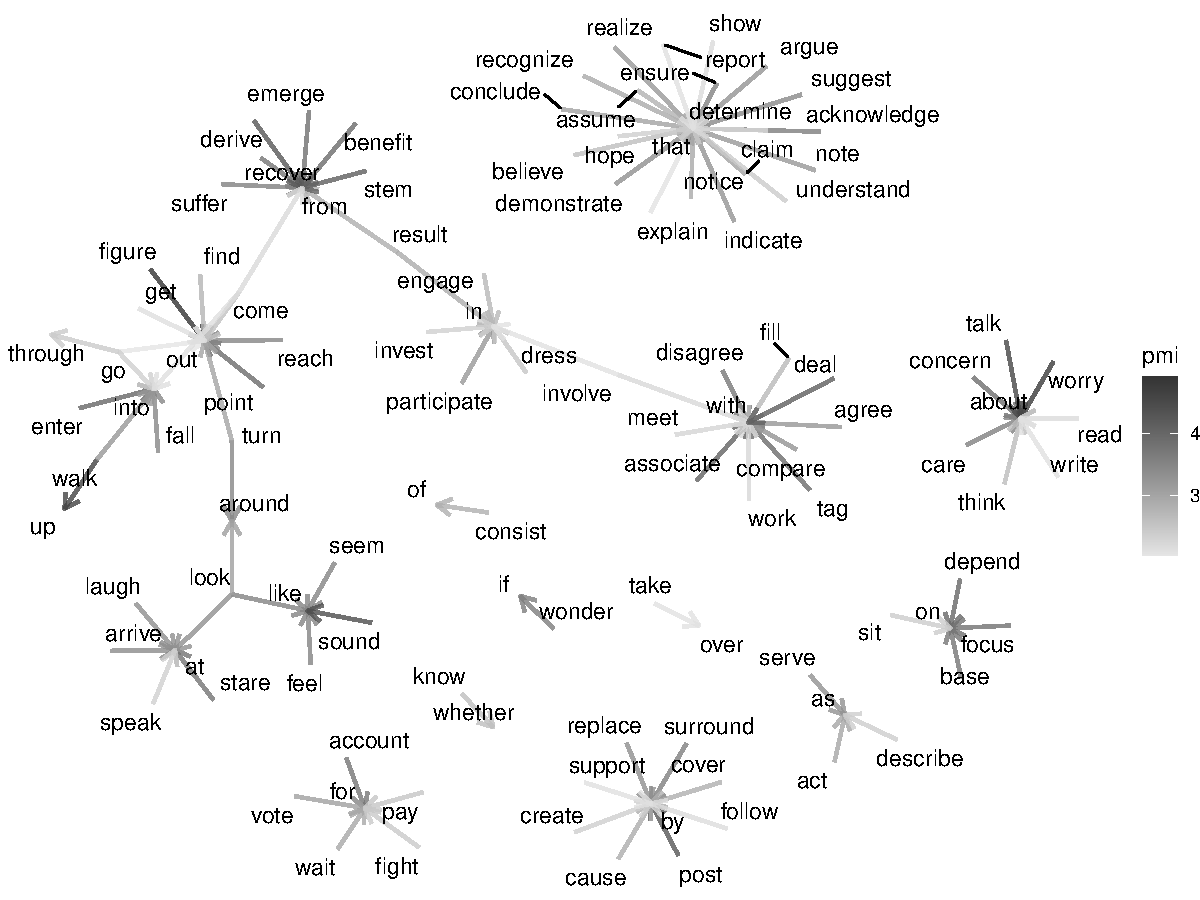
\includegraphics{part_4/8_explore_files/figure-pdf/fig-explore-masc-verb-part-network-1.pdf}

}

\caption{\label{fig-explore-masc-verb-part-network}Network plot of verb
particle constructions in the MASC dataset}

\end{figure}%

\begin{tcolorbox}[enhanced jigsaw, left=2mm, toprule=.15mm, colback=white, colframe=quarto-callout-color-frame, arc=.35mm, rightrule=.15mm, bottomrule=.15mm, leftrule=.75mm, breakable, opacityback=0]

\textbf{\faIcon{medal} Dive deeper}

\{ggplot2\} cannot create network plots directly, so we use \{ggraph\}
(\citeproc{ref-R-ggraph}{Pedersen, 2024}) and \{igraph\}
(\citeproc{ref-R-igraph}{Csárdi et al., 2024}) to create the network
plot. For more information on creating network plots, see the \{ggraph\}
documentation.

\end{tcolorbox}

From Figure~\ref{fig-explore-masc-verb-part-network}, and from the
underlying data, we can explore verb particle constructions. We could go
further and apply our co-occurrence methods to each modality separately,
if we wanted to identify verb particle constructions that are
distinctive to each modality. We could also apply our co-occurrence
methods to other parts-of-speech, such as adjectives and nouns, to
identify collocations of these parts-of-speech. There is much more to
explore with co-occurrence analysis, but this should give you a good
idea of the types of questions that can be addressed.

\subsection{Unsupervised learning}\label{sec-explore-unsupervised}

Aligned in purpose with descriptive approaches, unsupervised learning
approaches to exploratory data analysis are used to identify patterns in
the data from an algorithmic perspective. Common methods in text
analysis include principle component analysis, clustering, and vector
space modeling.

We will continue to use the MASC dataset as we develop materials for our
ELL textbook to illustrate unsupervised learning methods. In the
process, we will explore the following questions:

\begin{itemize}
\tightlist
\item
  Can we identify and group documents based on linguistic features or
  co-occurrence patterns of the data itself?
\item
  Do the groups of documents relate to categories in the dataset?
\item
  Can we estimate the semantics of words based on their co-occurrence
  patterns?
\end{itemize}

Through these questions we will build on our knowledge of frequency,
dispersion, and co-occurrence analysis and introduce concepts and
methods associated with machine learning.

\subsubsection{Clustering}\label{sec-explore-clustering}

\textbf{Clustering} is a unsupervised learning technique that can be
used to group similar items in the text data, helping to organize the
data into distinct categories and discover relationships between
different elements in the text. The main steps in the procedure includes
identifying the relevant linguistic features to use for clustering,
representing the features in a way that can be used for clustering,
applying a clustering algorithm to the data, and then interpreting the
results.

In our ELL textbook task, we may very well want to explore the
similiarities and/ or differences between the documents based on the
distribution of linguistic features. This provides us a view to evaluate
to what extent the variables in the dataset, say genre for this
demonstration, map to the distribution of linguistic features. Based on
this evaluation, we may want to consider re-categorizing the documents,
collapsing categories, or even adding new categories.

Instead of relying entirely on the variables' values in the MASC
dataset, we can let the data itself say something about how documents
may or may not be related. Yet, a pivotal question is what linguistic
features will use, otherwise known as \textbf{feature selection}. We
could use terms or lemmas, but we may want to consider other features,
such as parts of speech or some co-occurrence pattern. We are not locked
into using one criterion, and we can perform clustering multiple times
with different features, but we should consider the implications of our
feature selection for our interpretation of the results.

Imagine that among the various features that we are interested in
associating documents, we consider lemma use and POS use. However, we
need to operationalize what we mean by `use'. In machine learning, this
process is known as \textbf{feature engineering}. We likely want use
some measure of frequency. Since we are comparing documents, a relative
frequency measure will be most useful. Another consideration is what
does it mean to use lemmas or POS tags as our features. Each represents
a different linguistic of the documents. Lemmas represent the lexical
diversity of the documents while POS tags approximate the grammatical
diversity of the documents (\citeproc{ref-Petrenz2011}{Petrenz \&
Webber, 2011}).

Let's assume that our interest is to gauge the grammatical diversity of
the documents, so we will go with POS tags. With this approach, we aim
to distinguish between documents in a way that may allow us to use
consider whether genre-document categories are meaningful, along
grammatical lines.

The next question to address in any analysis is how to represent the
features. In machine learning, the most common way to represent
document- feature relationsips is in a matrix. In our case, we want to
create a matrix with the documents in the rows and the features in the
columns. The values in the matrix will be the operationalization of
grammatical diversity in each document. This configuration is known as a
\textbf{document-term matrix} (DTM).

To recast a data frame into a DTM, we can use the \texttt{cast\_dtm()}
function from \{tidytext\}. This function takes a data frame with a
document identifier, a feature identifier, and a value for each
observation and casts it into a matrix. Operations such as normalization
are easily and efficiently performed in R on matrices, so initially we
can cast a frequency table of POS tags into a matrix and then normalize
the matrix by documents.

Let's see how this works with the MASC dataset in
Example~\ref{exm-explore-masc-dtms}.

\begin{example}[]\protect\hypertarget{exm-explore-masc-dtms}{}\label{exm-explore-masc-dtms}

~

\begin{Shaded}
\begin{Highlighting}[]
\CommentTok{\# Load package}
\FunctionTok{library}\NormalTok{(tidytext)}

\CommentTok{\# Create a document{-}term matrix of POS tags}
\NormalTok{masc\_pos\_dtm }\OtherTok{\textless{}{-}}
\NormalTok{  masc\_tbl }\SpecialCharTok{|\textgreater{}}
  \FunctionTok{count}\NormalTok{(doc\_id, pos) }\SpecialCharTok{|\textgreater{}}
  \FunctionTok{cast\_dtm}\NormalTok{(doc\_id, pos, n) }\SpecialCharTok{|\textgreater{}}
  \FunctionTok{as.matrix}\NormalTok{()}

\CommentTok{\# Inpsect}
\FunctionTok{dim}\NormalTok{(masc\_pos\_dtm)}
\end{Highlighting}
\end{Shaded}

\begin{verbatim}
[1] 392  32
\end{verbatim}

\begin{Shaded}
\begin{Highlighting}[]
\CommentTok{\# Preview}
\NormalTok{masc\_pos\_dtm[}\DecValTok{1}\SpecialCharTok{:}\DecValTok{5}\NormalTok{, }\DecValTok{1}\SpecialCharTok{:}\DecValTok{5}\NormalTok{]}
\end{Highlighting}
\end{Shaded}

\begin{verbatim}
     Terms
Docs  CC DT EX IN JJ
  1   14 35  1 44 27
  10  11 38  0 39 18
  100  0  2  0  2  3
  101  3 16  0 23  7
  102 20 29  0 34 20
\end{verbatim}

\end{example}

The matrix \texttt{masc\_pos\_dtm} has 392 documents and 32 POS tags.
The values in the matrix are the frequency of each POS tag in each
document. Note preview the a subset of the contents of a matrix, such as
in Example~\ref{exm-explore-masc-dtms}, we use bracket syntax
\texttt{{[}{]}} instead of the \texttt{head()} function.

We can now normalize the matrix by documents. We can do this by dividing
each feature count by the total count in each document. This is a
row-wise transformation, so we can use the \texttt{rowSums()} function
from base R to calculate the total count in each document. Then each
count divided by its row's total count, as seen in
Example~\ref{exm-explore-masc-dtms-normalized}.

\begin{example}[]\protect\hypertarget{exm-explore-masc-dtms-normalized}{}\label{exm-explore-masc-dtms-normalized}

~

\begin{Shaded}
\begin{Highlighting}[]
\CommentTok{\# Normalize pos matrix by documents}
\NormalTok{masc\_pos\_dtm }\OtherTok{\textless{}{-}}
\NormalTok{  masc\_pos\_dtm }\SpecialCharTok{/} \FunctionTok{rowSums}\NormalTok{(masc\_pos\_dtm)}
\end{Highlighting}
\end{Shaded}

\end{example}

There are two concerns to address before we can proceed with clustering.
First, clustering algorithm performance tends to degrade with the number
of features. Second, clustering algorithms perform better with more
informative features. That is to say, features that are more distinct
across the documents provide better information for deriving useful
clusters.

We can address both of these concerns by reducing the number of features
and increasing the informativeness of the features. To accomplish this
is to use dimensionality reduction. \textbf{Dimensionality reduction} is
a set of methods that are used to reduce the number of features in a
dataset while retaining as much information as possible. The most common
method for dimensionality reduction is \textbf{principle component
analysis} (PCA). PCA is a method that transforms a set of correlated
variables into a set of uncorrelated variables, known as principle
components. The principle components are ordered by the amount of
variance that they explain in the data. The first principle component
explains the most variance, the second principle component explains the
second most variance, and so on.

We can apply PCA to the matrix and assess how well it accounts for the
variation in the data and how the variation is distributed across
components. The \texttt{prcomp()} function from base R can be used to
perform PCA.

Let's apply PCA to the matrix, as seen in
Example~\ref{exm-explore-masc-dtms-pca}.

\begin{example}[]\protect\hypertarget{exm-explore-masc-dtms-pca}{}\label{exm-explore-masc-dtms-pca}

~

\begin{Shaded}
\begin{Highlighting}[]
\CommentTok{\# Set seed}
\FunctionTok{set.seed}\NormalTok{(}\DecValTok{123}\NormalTok{)}

\CommentTok{\# Apply PCA to matrix}
\NormalTok{masc\_pos\_pca }\OtherTok{\textless{}{-}}
\NormalTok{  masc\_pos\_dtm }\SpecialCharTok{|\textgreater{}}
  \FunctionTok{prcomp}\NormalTok{()}
\end{Highlighting}
\end{Shaded}

\end{example}

We can visualize the amount of variance explained by each principle
component with a scree plot. A \textbf{scree plot} is a bar plot ordered
by the amount of variance explained by each principle component. The
\texttt{fviz\_eig()} function from \{factoextra\} implements a scree
plot on a PCA object. We can set the number of number of components to
visualize with \texttt{ncp\ =}.

\begin{example}[]\protect\hypertarget{exm-explore-masc-dtms-pca-scree}{}\label{exm-explore-masc-dtms-pca-scree}

~

\begin{Shaded}
\begin{Highlighting}[]
\CommentTok{\# Load package}
\FunctionTok{library}\NormalTok{(factoextra)}

\CommentTok{\# Scree plot: POS relative frequency}
\FunctionTok{fviz\_eig}\NormalTok{(masc\_pos\_pca, }\AttributeTok{ncp =} \DecValTok{10}\NormalTok{)}
\end{Highlighting}
\end{Shaded}

\begin{figure}[!htb]

\centering{

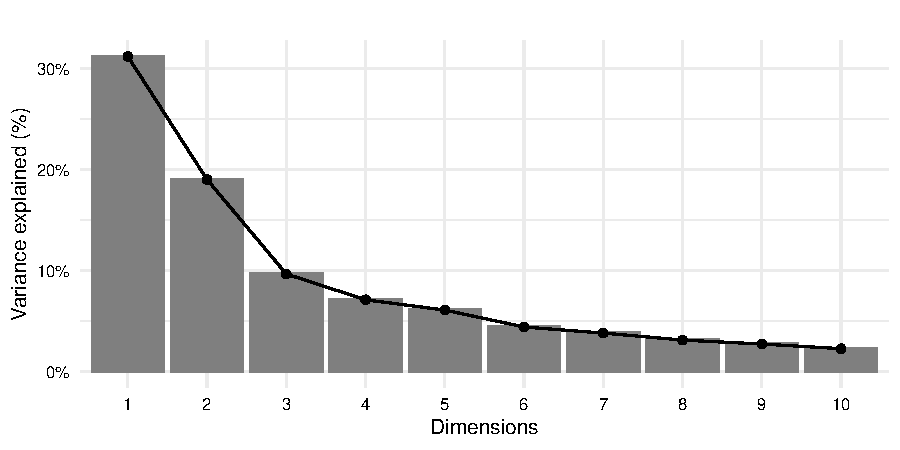
\includegraphics{part_4/8_explore_files/figure-pdf/fig-explore-masc-dtms-pca-scree-1.pdf}

}

\caption{\label{fig-explore-masc-dtms-pca-scree}Scree plot of the
principle components of the POS relative frequency}

\end{figure}%

\end{example}

\begin{tcolorbox}[enhanced jigsaw, left=2mm, toprule=.15mm, colback=white, colframe=quarto-callout-color-frame, arc=.35mm, rightrule=.15mm, bottomrule=.15mm, leftrule=.75mm, breakable, opacityback=0]

\textbf{\faIcon{medal} Dive deeper}

As with many modeling techniques we will encounter, it is possible to
extract the importance of features that contribute to the model. In the
case of PCA, we can extract the feature values from the principle
components using the \texttt{get\_pca\_var()} function from
\{factoextra\}. Feature importance provides more detailed insight into
the inner workings of the algorithms we employ in our research and
therefore can serve to inform our interpretation of the results.

\end{tcolorbox}

From the scree plot for the matrix, in
Figure~\ref{fig-explore-masc-dtms-pca-scree}, we can see that the first
component shows the most variance explained, around 30\%, and then drops
for subsequent drops as the number of dimensions increase. Visually we
will apply the elbow method to identify the number of dimensions to use
for clustering. It appears hhe variance explained decreases between 4
and 5 dimensions. This is a good indication that we should use 4
dimensions for our clustering algorithm.

Let's go ahead and create a matrix of the first four principle
components for the POS data, as seen in
Example~\ref{exm-explore-masc-pos-pca-pc}.

\begin{example}[]\protect\hypertarget{exm-explore-masc-pos-pca-pc}{}\label{exm-explore-masc-pos-pca-pc}

~

\begin{Shaded}
\begin{Highlighting}[]
\CommentTok{\# Create a matrix of the first four principle components}
\NormalTok{masc\_pos\_pca\_pc }\OtherTok{\textless{}{-}}
\NormalTok{  masc\_pos\_pca}\SpecialCharTok{$}\NormalTok{x[, }\DecValTok{1}\SpecialCharTok{:}\DecValTok{4}\NormalTok{]}
\end{Highlighting}
\end{Shaded}

\end{example}

Now that we have identified assessed the features that we want to use
for clustering and we have represented the features in a way that can be
used for clustering, we can apply a clustering algorithm to the data.

Some algorithms are better suited for certain types of data and certain
types of tasks. For example, \textbf{Hierarchical clustering} is a good
choice when we are not sure how many clusters we want to identify, as it
does not require us to specify the number of clusters from the outset.
However, it is not a good choice when we have a large dataset, as it can
be computationally expensive compared to some other algorithms.
\textbf{K-means clustering}, on the other hand, is a good choice when we
want to identify a pre-defined number of clusters, and the aim is to
gauge how well the data fit the clusters. These two clustering
techniques, therefore, complement each other with Hierarchical
clustering being a good choice for initial exploration and K-means
clustering being a good choice for targeted evaluation.

Since we are exploring the usefulness of the 18 genre labels used in the
MASC dataset we have a good idea of how many clusters we want to start
with. This is a good case to employ the K-means clustering algorithm.

In K-means clustering, we specify the number of clusters that we want to
identify. For each cluster number, a random center is generated. Then
each observation is assigned to the cluster with the nearest center. The
center of each cluster is then recalculated based on the distribution of
the observations in the cluster. This process is iterates either a
pre-defined number of times, or until the centers converge (\emph{i.e}
observations stop switching clusters).

The \texttt{kmeans()} function from base R takes the matrix of features
as its first argument and the number of clusters as its second argument.
We can specify the number of clusters with the \texttt{centers}
argument. Other arguments \texttt{nstart} and \texttt{iter.max} can be
used to specify the number of random starts and the maximum number of
iterations, respectively. Since the starting point for centers is
random, it is a good idea to run the algorithm multiple times with
different starting points. And we limit the interations to avoid the
algorithm running indefinitely.

Our goal, then, will be to assess how well this number of clusters fits
the data. After finding the optimal number of clusters, we can then
compare the results with the genre variable to see how well the clusters
map to the values of this variable.

One way to assess the fit of the clustering algorithm is to visualize
the results, interpret, and adjust the number of clusters, if necessary,
any number of times. Another, more efficient, approach is to
algorithmically assess the variability of the clusters based on
differing number of clusters and then select the number of clusters that
best fits the data.

We will take the later approach and plot the \textbf{within-cluster sum
of squares} (WSS) for a range of values for \(k\). The WSS is the sum of
the squared distance between each observation and its cluster center.
With a plot of the WSS for a range of values for \(k\), we can identify
the value for \(k\) where the WSS begins to level off, using the elbow
method. It is not always clear where the elbow is, yet it is a good
starting point for identifying the optimal number of clusters.

The \texttt{fviz\_nbclust()} function can be used to plot the WSS for a
range of values for \(k\). The \texttt{fviz\_nbclust()} function takes
the \texttt{kmeans()} function as its first argument and the matrix of
features as its second argument. The \texttt{fviz\_nbclust()} function
also takes arguments \texttt{method\ =\ "wss"} to specify the WSS method
and \texttt{k.max\ =\ 20} to specify the maximum number of clusters to
plot. Let's plot the WSS for a range of values for \(k\), as seen in
Figure~\ref{fig-explore-masc-pos-kmeans-elbow}.

\begin{Shaded}
\begin{Highlighting}[]
\NormalTok{masc\_pos\_pca\_pc }\SpecialCharTok{|\textgreater{}}
  \FunctionTok{fviz\_nbclust}\NormalTok{(}
    \AttributeTok{FUNcluster =}\NormalTok{ kmeans,}
    \AttributeTok{method =} \StringTok{"wss"}\NormalTok{, }\CommentTok{\# method}
    \AttributeTok{k.max =} \DecValTok{20}\NormalTok{,}
    \AttributeTok{nstart =} \DecValTok{25}\NormalTok{,}
    \AttributeTok{iter.max =} \DecValTok{20}
\NormalTok{  )}
\end{Highlighting}
\end{Shaded}

\begin{figure}[!htb]

\centering{

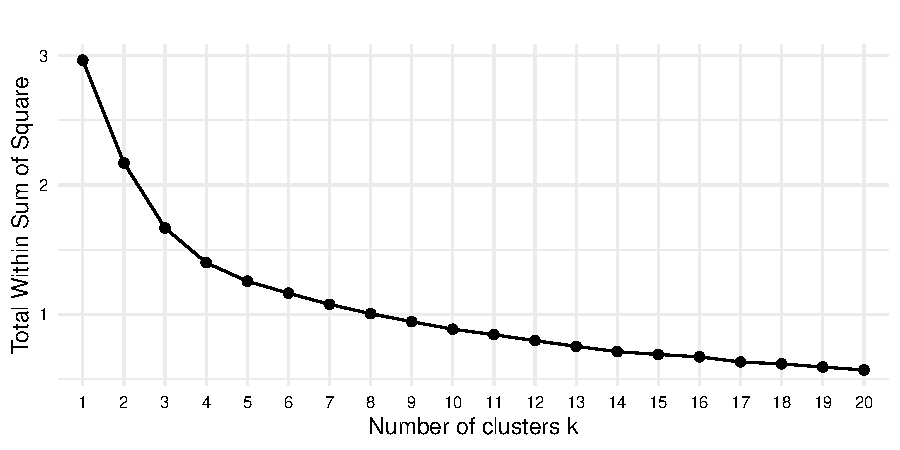
\includegraphics{part_4/8_explore_files/figure-pdf/fig-explore-masc-pos-kmeans-elbow-1.pdf}

}

\caption{\label{fig-explore-masc-pos-kmeans-elbow}Elbow method for
\(k\)-means clustering of the MASC dataset}

\end{figure}%

It is clear that there is significant gains in cluster fit from 1 to 4
clusters, but the gains begin to level off after 5-7 clusters.

Now we have an informed selection for \(k\). Let's use 4 clusters in the
\texttt{kmeans()} function and collect the results, as seen in
Example~\ref{exm-explore-masc-pos-kmeans-fit}.

\begin{example}[]\protect\hypertarget{exm-explore-masc-pos-kmeans-fit}{}\label{exm-explore-masc-pos-kmeans-fit}

~

\begin{Shaded}
\begin{Highlighting}[]
\CommentTok{\# Set seed}
\FunctionTok{set.seed}\NormalTok{(}\DecValTok{123}\NormalTok{)}

\CommentTok{\# K{-}means: for 4 clusters}
\NormalTok{masc\_pos\_kmeans\_fit }\OtherTok{\textless{}{-}}
\NormalTok{  masc\_pos\_pca\_pc }\SpecialCharTok{|\textgreater{}}
  \FunctionTok{kmeans}\NormalTok{(}
    \AttributeTok{centers =} \DecValTok{4}\NormalTok{,}
    \AttributeTok{nstart =} \DecValTok{25}\NormalTok{,}
    \AttributeTok{iter.max =} \DecValTok{20}
\NormalTok{  )}

\CommentTok{\# Preview}
\NormalTok{masc\_pos\_kmeans\_fit}\SpecialCharTok{$}\NormalTok{cluster[}\DecValTok{1}\SpecialCharTok{:}\DecValTok{10}\NormalTok{]}
\end{Highlighting}
\end{Shaded}

\begin{verbatim}
  1  10 100 101 102 103 104 105 106 107 
  1   1   2   3   3   2   2   2   4   3 
\end{verbatim}

\end{example}

The preview from Example~\ref{exm-explore-masc-pos-kmeans-fit} shows the
cluster assignments for the first 10 documents (\texttt{doc\_id}) in the
dataset.

From this point we can join document-cluster pairings produced by the
\(k\)-means algorithm with the original dataset. We can then explore the
clusters in terms of the original features. We can also explore the
clusters in terms of the original labels.

Let's join the cluster assignments to the original dataset, as seen in
Example~\ref{exm-explore-masc-pos-kmeans-join}.

\begin{example}[]\protect\hypertarget{exm-explore-masc-pos-kmeans-join}{}\label{exm-explore-masc-pos-kmeans-join}

~

\begin{Shaded}
\begin{Highlighting}[]
\CommentTok{\# Organize $k${-}means clusters into a tibble}
\NormalTok{masc\_pos\_cluster\_tbl }\OtherTok{\textless{}{-}}
  \FunctionTok{tibble}\NormalTok{(}
    \AttributeTok{doc\_id =} \FunctionTok{names}\NormalTok{(masc\_pos\_kmeans\_fit}\SpecialCharTok{$}\NormalTok{cluster),}
    \AttributeTok{cluster =}\NormalTok{ masc\_pos\_kmeans\_fit}\SpecialCharTok{$}\NormalTok{cluster}
\NormalTok{  )}

\CommentTok{\# Join cluster assignments to original dataset}
\NormalTok{masc\_cluster\_tbl }\OtherTok{\textless{}{-}}
\NormalTok{  masc\_tbl}\SpecialCharTok{|\textgreater{}}
  \FunctionTok{left\_join}\NormalTok{(}
\NormalTok{    masc\_pos\_cluster\_tbl,}
    \AttributeTok{by =} \StringTok{"doc\_id"}
\NormalTok{  )}

\CommentTok{\# Preview}
\NormalTok{masc\_cluster\_tbl }\SpecialCharTok{|\textgreater{}}
  \FunctionTok{slice\_head}\NormalTok{(}\AttributeTok{n =} \DecValTok{5}\NormalTok{)}
\end{Highlighting}
\end{Shaded}

\begin{verbatim}
# A tibble: 5 x 8
  doc_id modality genre   term_num term         lemma        pos   cluster
  <chr>  <chr>    <chr>      <dbl> <chr>        <chr>        <chr>   <int>
1 1      Written  Letters        2 Your         your         PRP$        1
2 1      Written  Letters        3 contribution contribution NN          1
3 1      Written  Letters        4 to           to           TO          1
4 1      Written  Letters        6 will         will         MD          1
5 1      Written  Letters        7 mean         mean         VB          1
\end{verbatim}

\end{example}

We now see that the cluster assignments from the \(k\)-means algorithm
have been joined to the original dataset. We can now explore the
clusters in terms of the original features. For example, let's look at
the distribution of the clusters across genre, as seen in
Example~\ref{exm-explore-masc-pos-kmeans-genre}. To do this, we first
need to reduce our dataset to the distinct combinations of genre and
cluster. Then, we can use \{janitor\}'s \texttt{tabyl()} function to
provided formatted percentages.

\begin{example}[]\protect\hypertarget{exm-explore-masc-pos-kmeans-genre}{}\label{exm-explore-masc-pos-kmeans-genre}

~

\begin{Shaded}
\begin{Highlighting}[]
\CommentTok{\# Load package}
\FunctionTok{library}\NormalTok{(janitor)}

\CommentTok{\# Reduce to distinct combinations of genre and cluster}
\NormalTok{masc\_meta\_tbl }\OtherTok{\textless{}{-}}
\NormalTok{  masc\_cluster\_tbl }\SpecialCharTok{|\textgreater{}}
  \FunctionTok{distinct}\NormalTok{(genre, cluster)}

\CommentTok{\# Tabulate: cluster by genre}
\NormalTok{masc\_meta\_tbl }\SpecialCharTok{|\textgreater{}}
  \FunctionTok{tabyl}\NormalTok{(genre, cluster) }\SpecialCharTok{|\textgreater{}}
  \FunctionTok{adorn\_totals}\NormalTok{(}\StringTok{"row"}\NormalTok{) }\SpecialCharTok{|\textgreater{}}
  \FunctionTok{adorn\_percentages}\NormalTok{(}\StringTok{"col"}\NormalTok{) }\SpecialCharTok{|\textgreater{}}
  \FunctionTok{adorn\_pct\_formatting}\NormalTok{(}\AttributeTok{digits =} \DecValTok{1}\NormalTok{) }\SpecialCharTok{|\textgreater{}}
  \FunctionTok{as\_tibble}\NormalTok{() }\SpecialCharTok{|\textgreater{}}
  \FunctionTok{tt}\NormalTok{(}\AttributeTok{width =} \DecValTok{1}\NormalTok{)}
\end{Highlighting}
\end{Shaded}

\begin{longtable}[]{@{}
  >{\raggedright\arraybackslash}p{(\columnwidth - 8\tabcolsep) * \real{0.2000}}
  >{\raggedright\arraybackslash}p{(\columnwidth - 8\tabcolsep) * \real{0.2000}}
  >{\raggedright\arraybackslash}p{(\columnwidth - 8\tabcolsep) * \real{0.2000}}
  >{\raggedright\arraybackslash}p{(\columnwidth - 8\tabcolsep) * \real{0.2000}}
  >{\raggedright\arraybackslash}p{(\columnwidth - 8\tabcolsep) * \real{0.2000}}@{}}

\caption{\label{tbl-explore-masc-pos-kmeans-genre}Distribution of
clusters by genre in the MASC dataset}

\tabularnewline

\toprule\noalign{}
\begin{minipage}[b]{\linewidth}\raggedright
genre
\end{minipage} & \begin{minipage}[b]{\linewidth}\raggedright
1
\end{minipage} & \begin{minipage}[b]{\linewidth}\raggedright
2
\end{minipage} & \begin{minipage}[b]{\linewidth}\raggedright
3
\end{minipage} & \begin{minipage}[b]{\linewidth}\raggedright
4
\end{minipage} \\
\midrule\noalign{}
\endhead
\bottomrule\noalign{}
\endlastfoot
Blog & 7.7\% & 20.0\% & 8.3\% & 0.0\% \\
Email & 7.7\% & 20.0\% & 8.3\% & 20.0\% \\
Essay & 7.7\% & 0.0\% & 8.3\% & 20.0\% \\
Face-to-face & 7.7\% & 0.0\% & 0.0\% & 0.0\% \\
Fiction & 7.7\% & 0.0\% & 8.3\% & 0.0\% \\
Fictlets & 7.7\% & 0.0\% & 0.0\% & 0.0\% \\
Government & 0.0\% & 0.0\% & 8.3\% & 0.0\% \\
Jokes & 7.7\% & 0.0\% & 0.0\% & 0.0\% \\
Journal & 7.7\% & 0.0\% & 8.3\% & 0.0\% \\
Letters & 7.7\% & 20.0\% & 8.3\% & 0.0\% \\
Movie Script & 7.7\% & 0.0\% & 8.3\% & 0.0\% \\
Newspaper & 7.7\% & 20.0\% & 8.3\% & 20.0\% \\
Non-fiction & 0.0\% & 0.0\% & 8.3\% & 20.0\% \\
Technical & 0.0\% & 0.0\% & 8.3\% & 20.0\% \\
Telephone & 7.7\% & 0.0\% & 0.0\% & 0.0\% \\
Transcript & 7.7\% & 0.0\% & 0.0\% & 0.0\% \\
Travel Guide & 0.0\% & 0.0\% & 8.3\% & 0.0\% \\
Twitter & 0.0\% & 20.0\% & 0.0\% & 0.0\% \\
Total & 100.0\% & 100.0\% & 100.0\% & 100.0\% \\

\end{longtable}

\end{example}

From Example~\ref{exm-explore-masc-pos-kmeans-genre}, we can see that
the clusters are not evenly distributed across the genres. In
particular, cluster 2 tends to be more associated with `blog', `email',
`letters', `twitter', and `news'. Another interesting cluster is cluster
4, which is more associated with `newspaper', `non-fiction', and
interestingly, `email'. This suggest that the clusters are capturing
some of the variation in the across the genres and potential within some
of the genres.

We could continue to explore genre, but we could also entertain the
possibility that the clusters may capture differences between modality
--even some interaction between modality and genre! This highlights how
exploratory data analysis through clustering can be used to identify new
questions and new variables of interest.

\begin{tcolorbox}[enhanced jigsaw, left=2mm, toprule=.15mm, colback=white, colframe=quarto-callout-color-frame, arc=.35mm, rightrule=.15mm, bottomrule=.15mm, leftrule=.75mm, breakable, opacityback=0]

\textbf{\faIcon{lightbulb} Consider this}

Given the cluster assignments derived using the distribution of POS
tags, what other relationships between the clusters and the original
features could one explore? What are the limitations of this approach?
What are the implications of this approach for the interpretation of the
results?

\end{tcolorbox}

\subsubsection{Vector space
models}\label{sec-explore-vector-space-models}

In our discussion of clustering, we targeted associations between
documents based on the distribution of linguistic features. We now turn
to targeting associations between linguistic features based on their
distribution across documents. The technique we will introduce is known
as \textbf{vector space modeling}. Vector space modeling aims to
represent linguistic features as numerical vectors which reflect the
various linguistic contexts in which the features appear. Together these
vectors form a feature-context space in which features with similar
contextual distributions are closer together.

An interesting property of vector space models is that are able to
capture semantic and/ or syntactic relationships between features based
on their distribution. In this way, vector space modeling can be seen as
an implementation of the \textbf{distributional hypothesis} --that is,
terms that appear in similar linguistic contexts tend to have similar
meanings (\citeproc{ref-Harris1954}{Harris, 1954}). As Firth
(\citeproc{ref-Firth1957}{1957}) states, ``you shall know a word by the
company it keeps''.

\begin{tcolorbox}[enhanced jigsaw, left=2mm, toprule=.15mm, colback=white, colframe=quarto-callout-color-frame, arc=.35mm, rightrule=.15mm, bottomrule=.15mm, leftrule=.75mm, breakable, opacityback=0]

\textbf{\faIcon{file-alt} Case study}

Garg, Schiebinger, Jurafsky, \& Zou (\citeproc{ref-Garg2018}{2018})
quantify and compare gender and ethnic stereotypes over time using word
embeddings. The authors explore the temporal dynamics of stereotypes
using word embeddings as a quantitative measure of bias. The data used
includes word embeddings from the Google News dataset for contemporary
analysis, as well as embeddings from the COHA and Google Books datasets
for historical analysis. Additional validation is done using embeddings
from the New York Times Annotated Corpus. Several word lists
representing gender, ethnicity, and neutral words are collated for
analysis. The main finding is that language reflects and perpetuates
cultural stereotypes, and the analysis shows consistency in the
relationships between embedding bias and external metrics across
datasets over time. The results also highlight the impact of historical
events, such as the women's movement of the 1960s, on the encoding of
stereotypes.

\end{tcolorbox}

Let's assume in our textbook project we are interested in gathering
information about English's expression of the semantic concepts of
manner and motion. For learners of English, this can be an area of
difficulty as languages differ in how these semantic properties are
expressed. English is a good example of a ``satellite-framed'' language,
that is that manner and motion are often encoded in the same verb with a
particle encoding the motion path (``rush out'', ``climb up''). Other
languages such as Spanish, Turkish, and Japanese are ``verb-framed''
languages, that is that motion but not manner is encoded in the verb
(``salir corriendo'', ``koşarak çıkmak'', ``走り出す'').

We can use vector space modeling to attempt to represent the
distribution of verbs in the MASC dataset and then target the concepts
of manner and motion to then explore how English encodes these concepts.
The question will be what will our features be. They could be terms,
lemmas, POS tags, \emph{etc}. Or they could be some combination.
Considering the task at hand which we will ultimately want to know
something about verbs, it makes sense to include the POS information in
combination with either the term or the lemma.

If we include term and POS then we have a feature for every
morphological variant of the term (\emph{e.g.} house\_VB, housed\_VBD,
housing\_VBG). This can make the model more sizeable than it needs to
be. If we include lemma and POS then we have a feature for every lemma
with a distinct grammatical category (\emph{e.g.} house\_NN, house\_VB).
Note that as the POS tags are from the Penn tagset, many morphological
variants appear in the tag itself (\emph{e.g.} house\_VB, houses\_VBZ,
housing\_VBG). This is a good example of how the choice of features can
impact the size of the model. In our case, it is not clear that we need
to include the morphological variants of the verbs, so I will use lemmas
and recode the POS variables as a simplified tagset.

After simplifying the features, we can then apply the vector space model
to the MASC dataset. When VSM is applied to words, it is known as
\textbf{word embedding}. To calculate word embeddings there are various
algorithms that can be used (BERT, word2vec, GloVe, \emph{etc.}) We will
use the \textbf{word2vec} (\citeproc{ref-Mikolov2013b}{Mikolov,
Sutskever, Chen, Corrado, \& Dean, 2013}) algorithm. Word2vec is a
neural network-based algorithm that learns word embeddings from a large
corpus of text. In the word2vec algorithm, the researcher can choose to
learn embeddings from a \textbf{Continuous Bag of Words} (CBOW) or a
\textbf{Skip-gram model}. The CBOW model predicts a target word based on
the context words. The Skip-gram model predicts the context words based
on the target word. The CBOW model is faster to train and is better for
frequent words. The Skip-gram model is slower to train and is better for
infrequent words.

\begin{tcolorbox}[enhanced jigsaw, left=2mm, toprule=.15mm, colback=white, colframe=quarto-callout-color-frame, arc=.35mm, rightrule=.15mm, bottomrule=.15mm, leftrule=.75mm, breakable, opacityback=0]

\textbf{\faIcon{medal} Dive deeper}

Choosing window size and dimensions for word2vec models is another
important consideration. The window size is the number of words that the
model will consider as context for the target word. Smaller window sizes
tend to capture more syntactic information, while larger window sizes
tend to capture more semantic information.

The number of dimensions is the number of features that the model will
learn. More dimensions can capture more information, but can also lead
to overfitting --picking up on nuances that are particular to the
dataset and that do not generalize well. Fewer dimensions can capture
less information, but can also lead to underfitting --not picking up on
nuances that are particular to the dataset and that do generalize well.
The number of dimensions is a hyperparameter that can be tuned to
optimize the model for the task at hand.

\end{tcolorbox}

Another consideration to take into account is the size of the corpus
used to train the model. VSM provide more reliable results when trained
on larger corpora. The MASC dataset is relatively small. We've
simplified our features in order to have a smaller vocabulary in hopes
to offset this limitation to a degree. But the choice of either CBOW or
Skip-gram can also help to offset this limitation. CBOW can be better
for smaller corpora as it aggregates context infomation. Skip-gram can
be better for larger corpora as it can capture more nuanced
relationships between words.

To implement the word2vec algorithm on our lemma + POS features, we will
use the \texttt{word2vec} package. The \texttt{word2vec()} function
takes a text file and uses it to train the vector representations. To
prepare the MASC dataset for training, we will need to write the lemma +
POS features to a text file as a single character string. We can do this
by first collapsing the \texttt{lemma\_pos} variable into a single
string for the entire corpus using the \texttt{str\_c()} function. Then
we can use the \texttt{write\_lines()} function to write the string to a
text file, as in Example~\ref{exm-explore-masc-vsm-write-txt}.

\begin{example}[]\protect\hypertarget{exm-explore-masc-vsm-write-txt}{}\label{exm-explore-masc-vsm-write-txt}

~

\begin{Shaded}
\begin{Highlighting}[]
\CommentTok{\# Write lemma + POS to text file}
\NormalTok{masc\_tbl }\SpecialCharTok{|\textgreater{}}
  \FunctionTok{summarize}\NormalTok{(}\AttributeTok{text =} \FunctionTok{str\_c}\NormalTok{(lemma\_pos, }\AttributeTok{collapse =} \StringTok{" "}\NormalTok{)) }\SpecialCharTok{|\textgreater{}}
  \FunctionTok{pull}\NormalTok{(text) }\SpecialCharTok{|\textgreater{}}
  \FunctionTok{write\_lines}\NormalTok{(}
    \AttributeTok{file =} \StringTok{"../data/analysis/masc\_lemma\_pos.txt"}
\NormalTok{  )}
\end{Highlighting}
\end{Shaded}

\end{example}

With the single line text file on disk, we will read it in, apply the
word2vec algorithm using the \texttt{word2vec} package, and write the
model to disk. By default, te \texttt{word2vec()} function applies the
CBOW model, with 50 dimensions, a window size of 5, and a minimum word
count of 5. We can change these parameters as needed, but let's apply
the default algorithm to the text file spliting features by sentence
punctuation, as seen in
Example~\ref{exm-explore-masc-vsm-word2vec-train}.

\begin{example}[]\protect\hypertarget{exm-explore-masc-vsm-word2vec-train}{}\label{exm-explore-masc-vsm-word2vec-train}

~

\begin{Shaded}
\begin{Highlighting}[]
\CommentTok{\# Load package}
\FunctionTok{library}\NormalTok{(word2vec)}

\CommentTok{\# Traing word2vec model}
\NormalTok{masc\_model }\OtherTok{\textless{}{-}}
  \FunctionTok{word2vec}\NormalTok{(}
    \AttributeTok{x =} \StringTok{"../data/analysis/masc\_lemma\_pos.txt"}\NormalTok{,}
    \AttributeTok{type =} \StringTok{"cbow"}\NormalTok{, }\CommentTok{\# or "skip{-}gram"}
    \AttributeTok{dim =} \DecValTok{100}\NormalTok{,}
    \AttributeTok{split =} \FunctionTok{c}\NormalTok{(}\StringTok{" "}\NormalTok{),}
    \AttributeTok{threads =} \DecValTok{8}\NormalTok{L}
\NormalTok{  )}

\CommentTok{\# Write model to disk}
\FunctionTok{write.word2vec}\NormalTok{(}
\NormalTok{  masc\_model,}
  \AttributeTok{file =} \StringTok{"../data/analysis/masc\_lemma\_pos.bin"}
\NormalTok{)}
\end{Highlighting}
\end{Shaded}

\end{example}

Writing the model to disk is important as it allows us to read the model
in without having to retrain it. In cases where the corpus is large,
this can save a lot of computational time.

Now that we have a trained model, we can read it in with the
\texttt{read.vectors()} function from \{wordVectors\}.

\begin{example}[]\protect\hypertarget{exm-explore-masc-vsm-word2vec-read}{}\label{exm-explore-masc-vsm-word2vec-read}

~

\begin{Shaded}
\begin{Highlighting}[]
\CommentTok{\# Load package}
\FunctionTok{library}\NormalTok{(wordVectors)}

\CommentTok{\# Read word2vec model}
\NormalTok{masc\_model }\OtherTok{\textless{}{-}}
  \FunctionTok{read.vectors}\NormalTok{(}
    \AttributeTok{filename =} \StringTok{"../data/analysis/masc\_lemma\_pos.bin"}
\NormalTok{  )}
\end{Highlighting}
\end{Shaded}

\end{example}

The \texttt{read.vectors()} function returns a matrix where each row is
a term in the model and each column is a dimension in the vector space,
as seen in Example~\ref{exm-explore-masc-vsm-word2vec-vector-object}.

\begin{example}[]\protect\hypertarget{exm-explore-masc-vsm-word2vec-vector-object}{}\label{exm-explore-masc-vsm-word2vec-vector-object}

~

\begin{Shaded}
\begin{Highlighting}[]
\CommentTok{\# Inspect}
\FunctionTok{dim}\NormalTok{(masc\_model)}
\end{Highlighting}
\end{Shaded}

\begin{verbatim}
[1] 5808  100
\end{verbatim}

\begin{Shaded}
\begin{Highlighting}[]
\CommentTok{\# Preview}
\NormalTok{masc\_model[}\DecValTok{1}\SpecialCharTok{:}\DecValTok{5}\NormalTok{, }\DecValTok{1}\SpecialCharTok{:}\DecValTok{5}\NormalTok{]}
\end{Highlighting}
\end{Shaded}

\begin{verbatim}
A VectorSpaceModel object of  5  words and  5  vectors
                   [,1]   [,2]    [,3]   [,4]    [,5]
abbreviated_ADJ   1.068  1.103 -0.3439  0.386 -1.0062
absent_ADJ       -1.839 -1.753  0.0658  0.119  0.9376
absorb_VERB      -1.772 -1.528 -0.0554  0.664 -1.2453
accidentally_ADV -1.264 -0.742 -0.6870  0.613 -1.0750
aesthetic_ADJ     0.567  0.524  1.0638 -0.332 -0.0424
attr(,".cache")
<environment: 0x7fc568651ba8>
\end{verbatim}

\end{example}

The row-wise vector in the model is the vector representation of each
feature. The notion is that these values can now be compared with other
features to explore distributional relatedness. We can extract specific
features from the matrix using the \texttt{{[}{]}} operator.

As an example, let's compare the vectors for noun-verb pairs for the
lemmas `run' and `walk'. To do this we extract these features from the
model. To appreciate the relatedness of these features it is best to
visualize them. We can do this by first reducing the dimensionality of
the vectors using principal components analysis. We can then plot the
first two principle components, as seen in
Figure~\ref{fig-explore-masc-vsm-word2vec-similarity}.

\begin{example}[]\protect\hypertarget{exm-explore-masc-vsm-word2vec-similarity}{}\label{exm-explore-masc-vsm-word2vec-similarity}

~

\begin{Shaded}
\begin{Highlighting}[]
\CommentTok{\# Extract vectors}
\NormalTok{word\_vectors }\OtherTok{\textless{}{-}}
\NormalTok{  masc\_model[}\FunctionTok{c}\NormalTok{(}\StringTok{"run\_VERB"}\NormalTok{, }\StringTok{"walk\_VERB"}\NormalTok{, }\StringTok{"run\_NOUN"}\NormalTok{, }\StringTok{"walk\_NOUN"}\NormalTok{), ] }\SpecialCharTok{|\textgreater{}}
  \FunctionTok{as.matrix}\NormalTok{()}

\CommentTok{\# Set seed for reproducibility}
\FunctionTok{set.seed}\NormalTok{(}\DecValTok{123}\NormalTok{)}

\NormalTok{pca }\OtherTok{\textless{}{-}}
\NormalTok{  word\_vectors }\SpecialCharTok{|\textgreater{}}
  \FunctionTok{scale}\NormalTok{() }\SpecialCharTok{|\textgreater{}}
  \FunctionTok{prcomp}\NormalTok{()}

\NormalTok{pca\_tbl }\OtherTok{\textless{}{-}}
  \FunctionTok{as\_tibble}\NormalTok{(pca}\SpecialCharTok{$}\NormalTok{x[, }\DecValTok{1}\SpecialCharTok{:}\DecValTok{2}\NormalTok{]) }\SpecialCharTok{|\textgreater{}}
  \FunctionTok{mutate}\NormalTok{(}\AttributeTok{word =} \FunctionTok{rownames}\NormalTok{(word\_vectors))}

\NormalTok{pca\_tbl }\SpecialCharTok{|\textgreater{}}
  \FunctionTok{ggplot}\NormalTok{(}\FunctionTok{aes}\NormalTok{(}\AttributeTok{x =}\NormalTok{ PC1, }\AttributeTok{y =}\NormalTok{ PC2, }\AttributeTok{label =}\NormalTok{ word)) }\SpecialCharTok{+}
  \FunctionTok{geom\_point}\NormalTok{() }\SpecialCharTok{+}
\NormalTok{  ggrepel}\SpecialCharTok{::}\FunctionTok{geom\_text\_repel}\NormalTok{()}
\end{Highlighting}
\end{Shaded}

\begin{figure}[!htb]

\centering{

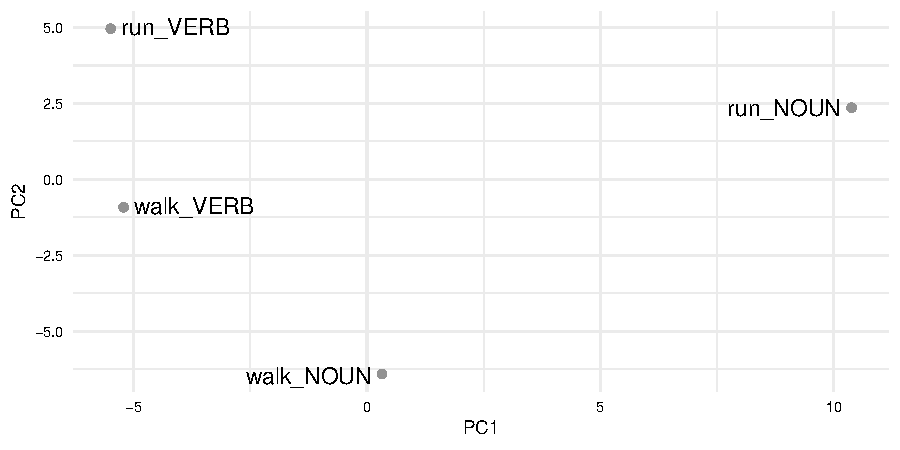
\includegraphics{part_4/8_explore_files/figure-pdf/fig-explore-masc-vsm-word2vec-similarity-1.pdf}

}

\caption{\label{fig-explore-masc-vsm-word2vec-similarity}Similarity
between `run' and `walk' in the MASC dataset}

\end{figure}%

\end{example}

From Figure~\ref{fig-explore-masc-vsm-word2vec-similarity}, we can see
that each of these features occupies a distinct position in the reduced
vector space. But on closer inspection, we can see that there is a
relationship between the lemma pairs. Remember that PCA reduces the
dimensionality of the data by identifying the dimensions that capture
the greatest amount of variance in the data. This means that of the 50
dimensions in the model, the PC1 and PC2 correspond to orthogonal
dimensions that capture the greatest amount of variance in the data. If
we look along PC1, we can see that there is a distinction between POS.
Looking along PC2, we see some pariety between lemma meanings. Given
these features, we can see that meaning and grammatical category can be
approximated in the vector space.

An interesting property of vector space models is that we can build up a
dimension of meaning by adding vectors that we expect to approximate
that meaning. For example, we can add the vectors for typical motion
verbs to create a vector for motion-similarity and one for
manner-similarity. We can then compare the feature vectors for all verbs
and assess their motion-similarity and manner-similarity.

To do this let's first subset the model to only include verbs, as in
Example~\ref{exm-explore-masc-vsm-word2vec-verbs}. We will also remove
the POS tags from the rownames of the matrix as they are no longer
needed.

\begin{example}[]\protect\hypertarget{exm-explore-masc-vsm-word2vec-verbs}{}\label{exm-explore-masc-vsm-word2vec-verbs}

~

\begin{Shaded}
\begin{Highlighting}[]
\CommentTok{\# Filter to verbs}
\NormalTok{verbs }\OtherTok{\textless{}{-}} \FunctionTok{str\_subset}\NormalTok{(}\FunctionTok{rownames}\NormalTok{(masc\_model), }\StringTok{".*\_VERB"}\NormalTok{)}
\NormalTok{verb\_vectors }\OtherTok{\textless{}{-}}\NormalTok{ masc\_model[verbs, ]}

\CommentTok{\# Remove POS tags}
\FunctionTok{rownames}\NormalTok{(verb\_vectors) }\OtherTok{\textless{}{-}}
\NormalTok{  verb\_vectors }\SpecialCharTok{|\textgreater{}}
  \FunctionTok{rownames}\NormalTok{() }\SpecialCharTok{|\textgreater{}}
  \FunctionTok{str\_replace\_all}\NormalTok{(}\StringTok{"\_VERB"}\NormalTok{, }\StringTok{""}\NormalTok{)}

\CommentTok{\# Inspect}
\FunctionTok{dim}\NormalTok{(verb\_vectors)}
\end{Highlighting}
\end{Shaded}

\begin{verbatim}
[1] 1115  100
\end{verbatim}

\begin{Shaded}
\begin{Highlighting}[]
\CommentTok{\# Preview}
\NormalTok{verb\_vectors[}\DecValTok{1}\SpecialCharTok{:}\DecValTok{5}\NormalTok{, }\DecValTok{1}\SpecialCharTok{:}\DecValTok{5}\NormalTok{]}
\end{Highlighting}
\end{Shaded}

\begin{verbatim}
A VectorSpaceModel object of  5  words and  5  vectors
          [,1]   [,2]    [,3]    [,4]   [,5]
absorb  -1.772 -1.528 -0.0554  0.6642 -1.245
auction -2.083 -0.977 -0.2505 -0.0204 -0.874
bid      0.217 -0.490 -0.4588  0.1373  0.247
brief    1.215 -0.674 -0.7121  0.5072 -0.445
cap     -0.135  0.884  0.2278 -0.2563 -0.207
attr(,".cache")
<environment: 0x7fc543f4ed38>
\end{verbatim}

\end{example}

We now have \texttt{verb\_vectors} which includes the vector
representations for all verbs 1,115 in the MASC dataset. Next, let's
seed the vectors for motion-similarity and manner-similarity and
calculate the vector `closeness' to the motion and manner seed vectors
with the \texttt{closest\_to()} function from the \texttt{wordVectors()}
package.

\begin{example}[]\protect\hypertarget{exm-explore-masc-vsm-word2vec-manner-motion}{}\label{exm-explore-masc-vsm-word2vec-manner-motion}

~

\begin{Shaded}
\begin{Highlighting}[]
\CommentTok{\# Add vectors for motion{-}similarity and manner{-}similarity}
\NormalTok{motion }\OtherTok{\textless{}{-}}
  \FunctionTok{c}\NormalTok{(}\StringTok{"go"}\NormalTok{, }\StringTok{"come"}\NormalTok{, }\StringTok{"leave"}\NormalTok{, }\StringTok{"arrive"}\NormalTok{, }\StringTok{"enter"}\NormalTok{, }\StringTok{"exit"}\NormalTok{, }\StringTok{"depart"}\NormalTok{, }\StringTok{"return"}\NormalTok{)}

\NormalTok{motion\_similarity }\OtherTok{\textless{}{-}}
\NormalTok{  verb\_vectors }\SpecialCharTok{|\textgreater{}} \FunctionTok{closest\_to}\NormalTok{(motion, }\AttributeTok{n =} \ConstantTok{Inf}\NormalTok{)}

\CommentTok{\# Preview}
\NormalTok{motion\_similarity }\SpecialCharTok{|\textgreater{}} \FunctionTok{glimpse}\NormalTok{()}
\end{Highlighting}
\end{Shaded}

\begin{verbatim}
Rows: 1,115
Columns: 2
$ word                   <chr> "walk", "step", "return", "enter", "leave", "le~
$ `similarity to motion` <dbl> 0.742, 0.741, 0.732, 0.727, 0.682, 0.669, 0.664~
\end{verbatim}

\begin{Shaded}
\begin{Highlighting}[]
\NormalTok{manner }\OtherTok{\textless{}{-}}
  \FunctionTok{c}\NormalTok{(}\StringTok{"run"}\NormalTok{, }\StringTok{"walk"}\NormalTok{, }\StringTok{"jump"}\NormalTok{, }\StringTok{"crawl"}\NormalTok{, }\StringTok{"swim"}\NormalTok{, }\StringTok{"fly"}\NormalTok{, }\StringTok{"drive"}\NormalTok{, }\StringTok{"ride"}\NormalTok{)}

\NormalTok{manner\_similarity }\OtherTok{\textless{}{-}}
\NormalTok{  verb\_vectors }\SpecialCharTok{|\textgreater{}} \FunctionTok{closest\_to}\NormalTok{(manner, }\AttributeTok{n =} \ConstantTok{Inf}\NormalTok{)}

\CommentTok{\# Preview}
\NormalTok{manner\_similarity }\SpecialCharTok{|\textgreater{}} \FunctionTok{glimpse}\NormalTok{()}
\end{Highlighting}
\end{Shaded}

\begin{verbatim}
Rows: 1,115
Columns: 2
$ word                   <chr> "walk", "drop", "step", "hang", "rub", "shut", ~
$ `similarity to manner` <dbl> 0.865, 0.841, 0.831, 0.826, 0.826, 0.824, 0.820~
\end{verbatim}

\end{example}

The \texttt{motion\_similarity} and \texttt{manner\_similarity} data
frames each contain all the verbs with a corresponding closeness
measure. We can join these two data frames by feature to create a single
data frame with the motion-similarity and manner-similarity measures, as
seen in Example~\ref{exm-explore-masc-vsm-word2vec-manner-motion}.

\begin{example}[]\protect\hypertarget{exm-explore-masc-vsm-word2vec-manner-motion}{}\label{exm-explore-masc-vsm-word2vec-manner-motion}

~

\begin{Shaded}
\begin{Highlighting}[]
\CommentTok{\# Join motion{-}similarity and manner{-}similarity}
\NormalTok{manner\_motion\_similarity }\OtherTok{\textless{}{-}}
\NormalTok{  manner\_similarity }\SpecialCharTok{|\textgreater{}}
  \FunctionTok{inner\_join}\NormalTok{(motion\_similarity)}

\CommentTok{\# Preview}
\NormalTok{manner\_motion\_similarity }\SpecialCharTok{|\textgreater{}} \FunctionTok{glimpse}\NormalTok{()}
\end{Highlighting}
\end{Shaded}

\begin{verbatim}
Rows: 1,115
Columns: 3
$ word                   <chr> "walk", "drop", "step", "hang", "rub", "shut", ~
$ `similarity to manner` <dbl> 0.865, 0.841, 0.831, 0.826, 0.826, 0.824, 0.820~
$ `similarity to motion` <dbl> 0.742, 0.642, 0.741, 0.635, 0.624, 0.589, 0.561~
\end{verbatim}

\end{example}

The result of Example~\ref{exm-explore-masc-vsm-word2vec-manner-motion}
is a data frame with the motion-similarity and manner-similarity
measures for all verbs in the MASC dataset. We can now visualize the
distribution of motion-similarity and manner-similarity measures, as
seen in
Figure~\ref{fig-explore-masc-vsm-word2vec-manner-motion-compare}.

\begin{figure}[!htb]

\centering{

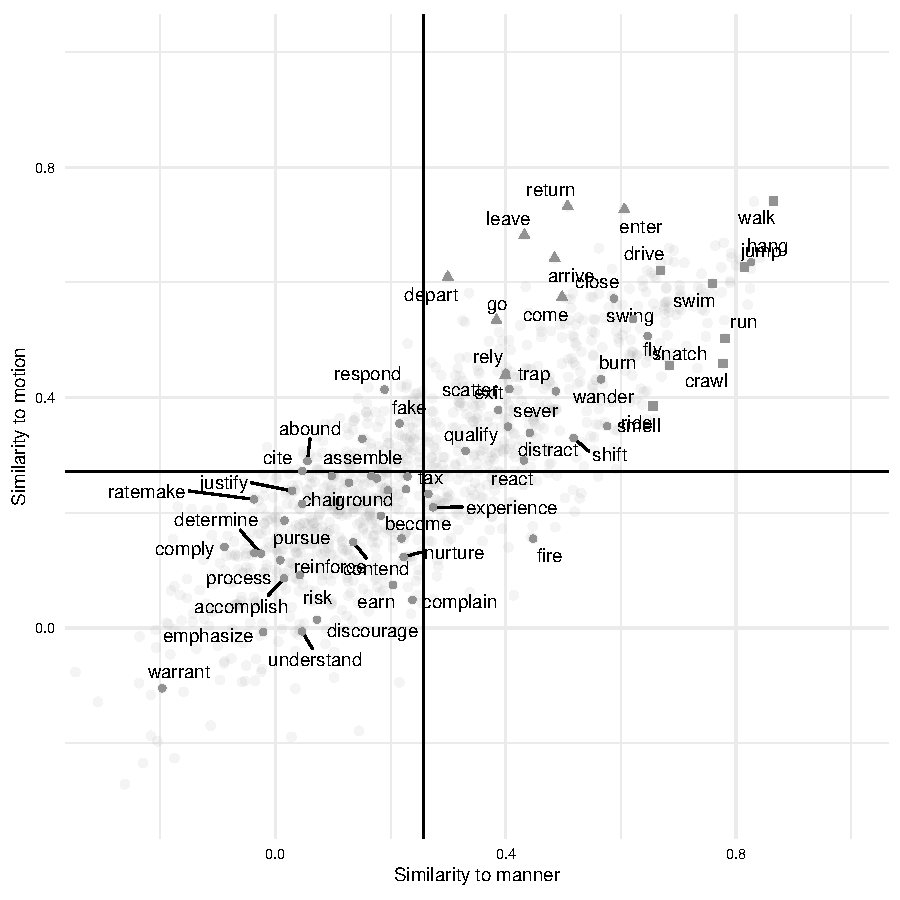
\includegraphics{part_4/8_explore_files/figure-pdf/fig-explore-masc-vsm-word2vec-manner-motion-compare-1.pdf}

}

\caption{\label{fig-explore-masc-vsm-word2vec-manner-motion-compare}Motion-similarity
and manner-similarity of verbs in the MASC dataset}

\end{figure}%

From Figure~\ref{fig-explore-masc-vsm-word2vec-manner-motion-compare},
we can see that the manner-similarity is plotted on the x-axis and the
motion-similarity on the y-axis. I've added horizontal and vertical
lines to break the scatterplot into quadrants --the top-right
corresponding to high manner- and motion-similiarity and the bottom-left
corresponding to low manner- and motion-similarity. This captures the
majority of the verbs in the dataset. The verbs in the top-left quadrant
have high motion-similarity but lower manner similarity, and verbs in
the bottom-right quadrant have high manner-similarity but lower
motion-similarity.

I've randomly sampled 50 verbs from the dataset and plotted them as text
labels. I've also plotted the motion and manner seed vectors as triangle
and box points, respectively. We can see that motion- and
manner-similiarity seed verbs are found in the top-left quandrant
together, showing that they are semantically related. Verbs in the other
quadrants are either lower in motion- or manner-similarity, or both.
From a qualitative point of view it appears that many of the verbs
coincide with inuition. Some, however, less so. This is to be expected
to some degree as the model is trained on a relatively small corpus. All
in all, this serves as an example of how vector space modeling can be
used to explore semantic relationships between linguistic features.

\section*{Activities}\label{activities-6}
\addcontentsline{toc}{section}{Activities}

\markright{Activities}

Exploratory analysis is a wide-ranging term that encompasses many
different methods. In these activities, we will focus on the methods
that are most commonly used in the analysis of textual data. These
include frequency and distributional analysis, clustering, and word
embedding models. We will model how to explore iteratively using the
output of one method to inform the next and ultimately to address a
research question.

\begin{tcolorbox}[enhanced jigsaw, left=2mm, toprule=.15mm, colback=white, colframe=quarto-callout-color-frame, arc=.35mm, rightrule=.15mm, bottomrule=.15mm, leftrule=.75mm, breakable, opacityback=0]

\textbf{\faIcon{file-code} Recipe}

\textbf{What}: Exploratory analysis methods\\
\textbf{How}: Read Recipe 8, complete comprehension check, and prepare
for Lab 8.\\
\textbf{Why}: To illustrate how to prepare a dataset for descriptive and
unsupervised machine learning methods and evaluate the results for
exploratory data analysis.

\end{tcolorbox}

\begin{tcolorbox}[enhanced jigsaw, left=2mm, toprule=.15mm, colback=white, colframe=quarto-callout-color-frame, arc=.35mm, rightrule=.15mm, bottomrule=.15mm, leftrule=.75mm, breakable, opacityback=0]

\textbf{\faIcon{flask} Lab}

\textbf{What}: Pattern discovery\\
\textbf{How}: Clone, fork, and complete the steps in Lab 8.\\
\textbf{Why}: To gain experience working with coding strategies to
prepare, feature engineer, explore, and evaluate results from
exploratory data analyses, practice transforming datasets into new
object formats and visualizing relationships, and implement
organizational strategies for organizing and reporting results in a
reproducible fashion.

\end{tcolorbox}

\section*{Summary}\label{summary-7}
\addcontentsline{toc}{section}{Summary}

\markright{Summary}

In this chapter, we surveyed a range of methods for uncovering insights
from data, particularly when we do not have a predetermined hypothesis.
We broke the chapter discussion along the two central branches of
exploratory data analysis: descriptive analysis and unsupervised
learning. Descriptive analysis offers statistical or visual summaries of
datasets through frequency, dispersion, and co-occurrence measures,
while unsupervised learning utilizes machine learning techniques to
uncover patterns without predefining variable relationships. Here we
covered a few unsupervised learning methods including clustering,
diminensionality reduction, and vector space modeling. Through either
descriptive or unsupervised learning methodologies, we probe questions
in a data-driven fashion and apply methods to summarize, reduce, and
sort complex datasets. This in turn facilitates novel, quantitative
perspectives that can subsequently be evaluated qualitatively, offering
us a robust approach to exploring and generating research questions.

\chapter{Predict}\label{sec-predict-chapter}

\begin{quote}
All models are wrong, but some are useful.

--- George E.P. Box
\end{quote}

\begin{tcolorbox}[enhanced jigsaw, left=2mm, toprule=.15mm, colback=white, colframe=quarto-callout-color-frame, arc=.35mm, rightrule=.15mm, bottomrule=.15mm, leftrule=.75mm, breakable, opacityback=0]

\textbf{\faIcon{list-alt} Outcomes}

\begin{itemize}
\tightlist
\item
  Identify the research goals of predictive data analysis
\item
  Describe the workflow for predictive data analysis
\item
  Recognize quantitative and qualitative methods for evaluating
  predictive models
\end{itemize}

\end{tcolorbox}

In this chapter, I introduce supervised learning as an approach to text
analysis. Supervised learning aims to establish a relationship between a
target (or outcome) variable and a set of feature variables derived from
text data. By leveraging this relationship, statistical generalizations
(models) can be created to accurately predict values of the target
variable based on the values of the feature variables. Throughout the
chapter, we explore practical tasks and theoretical applications of
statistical learning in text analysis.

\begin{tcolorbox}[enhanced jigsaw, left=2mm, toprule=.15mm, colback=white, colframe=quarto-callout-color-frame, arc=.35mm, rightrule=.15mm, bottomrule=.15mm, leftrule=.75mm, breakable, opacityback=0]

\textbf{\faIcon{terminal} Lessons}

\textbf{What}: Advanced Visualization\\
\textbf{How}: In an R console, load \{swirl\}, run \texttt{swirl()}, and
follow prompts to select the lesson.\\
\textbf{Why}: To dive deeper into \{ggplot2\} to enhance visual
summaries and provides an introduction to \{factoextra\} and
\{ggfortify\} that extend \{ggplot2\} capabilities to model objects.

\end{tcolorbox}

\section{Orientation}\label{sec-predict-orientation}

Predictive data analysis (PDA) is a powerful analysis method for making
predictions about new or future data based on patterns in existing data.
PDA is a type of supervised learning, which means that it involves
training a model on a labeled dataset where the input data and desired
output are both provided. The model is able to make predictions or
classifications based on the input data by learning the relationships
between the input and output data. Supervised machine learning is an
important tool for linguists studying language and communication, as it
allows us to analyze language data to identify patterns or trends in
language use, assess hypotheses, and prescribe actions.

The approach to conducting predictive analysis shares some commonalities
with exploratory data analysis (Section~\ref{sec-explore-orientation})
(as well as inferential analysis Chapter~\ref{sec-infer-chapter}), but
there are also some key differences. Consider the workflow in
Table~\ref{tbl-predict-workflow}.

\begin{longtable}[]{@{}
  >{\raggedright\arraybackslash}p{(\columnwidth - 4\tabcolsep) * \real{0.0500}}
  >{\raggedright\arraybackslash}p{(\columnwidth - 4\tabcolsep) * \real{0.1500}}
  >{\raggedright\arraybackslash}p{(\columnwidth - 4\tabcolsep) * \real{0.8000}}@{}}
\caption{Workflow for predictive data
analysis}\label{tbl-predict-workflow}\tabularnewline
\toprule\noalign{}
\begin{minipage}[b]{\linewidth}\raggedright
Step
\end{minipage} & \begin{minipage}[b]{\linewidth}\raggedright
Name
\end{minipage} & \begin{minipage}[b]{\linewidth}\raggedright
Description
\end{minipage} \\
\midrule\noalign{}
\endfirsthead
\toprule\noalign{}
\begin{minipage}[b]{\linewidth}\raggedright
Step
\end{minipage} & \begin{minipage}[b]{\linewidth}\raggedright
Name
\end{minipage} & \begin{minipage}[b]{\linewidth}\raggedright
Description
\end{minipage} \\
\midrule\noalign{}
\endhead
\bottomrule\noalign{}
\endlastfoot
1 & Identify & Consider the research question and aim and identify
relevant variables \\
2 & & Split the data into representative training and testing sets \\
3 & & Apply variable selection and engineering procedures \\
4 & Inspect & Inspect the data to ensure that it is in the correct
format and that the training and testing sets are representative of the
data \\
5 & Interrogate & Train and evaluate the model on the training set,
adjusting models or hyperparameters as needed, to produce a final
model \\
6 & (Optional) Iterate & Repeat steps 3-5 to selecting new variables,
models, hyperparameters \\
7 & Interpret & Interpret the results of the final model in light of the
research question or hypothesis \\
\end{longtable}

Focusing on the overlap with other analysis methods, we can see some
fundamentals steps such as identifying relevant variables, inspecting
the data, interrogating the data, and interpreting the results. And if
our research aim is exploratory in nature, iteration may also be a part
of the workflow.

There are two main differences, however, between the PDA and the EDA
workflow we discussed in Chapter~\ref{sec-explore-chapter}. The first,
reflected the majority of the steps in the workflow, is that PDA
requires partitioning the data into training and testing sets. The
training set is used to develop the model, and the testing set is used
to evaluate the model's performance. This strategy is used to ensure
that the model is robust and generalizes well to new data. It is well
known, and makes intuitive sense, that using the same data to develop
and evaluate a model likely will not produce a model that generalizes
well to new data. This is because the model will have potentially
conflated the nuances of the data (`the noise') with any real trends
(`the signal') and therefore will not be able to generalize well to new
data. This is called \textbf{overfitting} and by holding out a portion
of the data for testing, we can evaluate the model's performance on data
that it has not seen before and therefore get a more accurate estimate
of the generalizable trends in the data.

\begin{tcolorbox}[enhanced jigsaw, left=2mm, toprule=.15mm, colback=white, colframe=quarto-callout-color-frame, arc=.35mm, rightrule=.15mm, bottomrule=.15mm, leftrule=.75mm, breakable, opacityback=0]

\textbf{\faIcon{medal} Dive deeper}

Prediction modeling is a hot topic. Given the potential to make
actionable predictions about future outcomes, it attracts a lot of
attention from organizations which aim to leverage data to make informed
decisions. It's use in research is also growing beyond the development
of better models and using predictive models to address research
questions and hypotheses.

We will apply predictive modeling in the context of language data as a
semi-inductive method. However, it is also increasingly used in
hypothesis testing scenarios, see S. Th. Gries \& Deshors
(\citeproc{ref-Gries2014}{2014}), Deshors \& Gries
(\citeproc{ref-Deshors2016}{2016}), and R. Harald Baayen
(\citeproc{ref-Baayen2011}{2011}) for examples.

\end{tcolorbox}

Another procedure to avoid the perils of overfitting, is to use
resampling methods as part of the model evaluation on the training set.
Resampling is the process of repeatedly drawing samples from the
training set and evaluating the model on each sample. The two most
common resampling methods are \textbf{bootstrapping} (resampling with
replacement) and \textbf{cross-validation} (resampling without
replacement). The performance of these multiple models are summarized
and the error between them is assessed. The goal is to minimize the
performance differences between the models while maximizing the overall
performance. These measures go a long way to avoiding overfitting and
therefore maximizing the chance that the training phase will produce a
model which is robust at the testing phase.

The second difference, not reflected in the workflow but inherent in
predictive analysis, is that PDA requires a fixed outcome variable. This
means that the outcome variable must be defined from the outset and
cannot be changed during the analysis. Furthermore, the informational
nature of the outcome variable will dictate the what type of algorithm
we choose to interrogate the data and how we will evaluate the model's
performance.

If the outcome is categorical in nature, we will use a
\textbf{classification algorithm} (\emph{e.g.} logistic regression,
naive bayes, \emph{etc.}). Classification evaluation metrics include
accuracy, precision, recall, and F1 score which can be derived from and
visualized in a cross-tabulation of the predicted and actual outcome
values.

If the outcome is numeric in nature, we will use a \textbf{regression
algorithm} (\emph{e.g.} linear regression, support vector regression,
\emph{etc.}). Since the difference between prediction and actual values
is numeric, metrics that quantify numerical differences, such as root
mean square error (RMSE) or \(R^2\), are used to evaluate the model's
performance.

The evaluation of the model is quantitative on the one hand, but it is
also qualitative in that we need to consider the implications of the
model's performance in light of the research question or hypothesis.
Furthermore, depending on our research question we may be interested in
exploring the features that are most important to the model's
performance. This is called \textbf{feature importance} and can be
derived from the model's coefficients or weights. Notably, however, some
of the most powerful models in use today, such as deep neural networks,
are not easily interpretable and therefore feature importance is not
easily derived. This is something to keep in mind when considering the
research question and the type of model that will be used to address it.

\section{Analysis}\label{sec-predict-analysis}

In this section, we now turn to the practical application of predictive
data analysis. The discussion will be separated into classification and
regression tasks, as model selection and evaluation procedures differ
between the two. For each task, we will frame a research goal and work
through the process of building a predictive model to address that goal.
Along the way we will cover concepts and methods that are common to both
classification and regression tasks and specific to each.

To frame our analyses, we will posit research aimed at identifying
language usage patterns in second language use, one for a classification
task and one for a regression task. Our first research question will be
to assess whether we Spanish language use can be used to predict natives
and L1 English learners (categorical). Our second research question will
be to gauge the extent to which the the L1 English learners' Spanish
language placement test scores (numeric) can be predicted based on their
language use.

We will use data from the CEDEL2 corpus
(\citeproc{ref-Lozano2009}{Lozano, 2009}). We will include a subset of
the variables from this data that are relevant to our research
questions. The data dictionary for this dataset is seen in
Table~\ref{tbl-predict-cedel2-data-dictionary}.

\begin{longtable}[]{@{}
  >{\raggedright\arraybackslash}p{(\columnwidth - 6\tabcolsep) * \real{0.1500}}
  >{\raggedright\arraybackslash}p{(\columnwidth - 6\tabcolsep) * \real{0.1500}}
  >{\raggedright\arraybackslash}p{(\columnwidth - 6\tabcolsep) * \real{0.1500}}
  >{\raggedright\arraybackslash}p{(\columnwidth - 6\tabcolsep) * \real{0.5500}}@{}}

\caption{\label{tbl-predict-cedel2-data-dictionary}Data dictionary for
the CEDEL2 corpus}

\tabularnewline

\toprule\noalign{}
\begin{minipage}[b]{\linewidth}\raggedright
variable
\end{minipage} & \begin{minipage}[b]{\linewidth}\raggedright
name
\end{minipage} & \begin{minipage}[b]{\linewidth}\raggedright
type
\end{minipage} & \begin{minipage}[b]{\linewidth}\raggedright
description
\end{minipage} \\
\midrule\noalign{}
\endhead
\bottomrule\noalign{}
\endlastfoot
doc\_id & Document ID & numeric & Unique identifier for each document \\
subcorpus & Subcorpus & categorical & The subcorpus to which the
document belongs (`Learner' or `Native') \\
placement\_score & Placement Score & numeric & The score obtained by the
document author in a placement test. Null values indicate missing data
(i.e.~the document author did not take the placement test) \\
proficiency & Proficiency & ordinal & The level of language proficiency
of the document author (`Upper intermediate', `Lower advanced', `Upper
beginner', or `Native') \\
text & Text & character & The written text provided by the document
author \\

\end{longtable}

Let's go ahead and read the transformed dataset and preview it in
Example~\ref{exm-predict-cedel-read}.

\begin{example}[]\protect\hypertarget{exm-predict-cedel-read}{}\label{exm-predict-cedel-read}

~

\begin{Shaded}
\begin{Highlighting}[]
\CommentTok{\# Read in the dataset}
\NormalTok{cedel\_tbl}\OtherTok{\textless{}{-}}
  \FunctionTok{read\_csv}\NormalTok{(}\StringTok{"../data/cedel2/cedel2\_transformed.csv"}\NormalTok{)}

\CommentTok{\# Preview}
\NormalTok{cedel\_tbl }\SpecialCharTok{|\textgreater{}} \FunctionTok{glimpse}\NormalTok{()}
\end{Highlighting}
\end{Shaded}

\begin{verbatim}
Rows: 2,957
Columns: 5
$ doc_id          <dbl> 1, 2, 3, 4, 5, 6, 7, 8, 9, 10, 11, 12, 13, 14, 15, 16,~
$ subcorpus       <chr> "Learner", "Learner", "Learner", "Learner", "Learner",~
$ placement_score <dbl> 14.0, 16.3, 16.3, 18.6, 18.6, 18.6, 20.9, 20.9, 20.9, ~
$ proficiency     <chr> "Lower beginner", "Lower beginner", "Lower beginner", ~
$ text            <chr> "Yo vivo es Alanta, Georgia. Atlanta es muy grande ciu~
\end{verbatim}

\end{example}

The output of Example~\ref{exm-predict-cedel-read} provides some
structural information about the dataset, number of rows and columns as
well as variable types.

After I performed some diagnostics and made some adjustments, the
dataset is in good order to proceed with the analysis. I updated the
variables \texttt{subcorpus} and \texttt{proficiency} as factor
variables and ordered them in a way that makes sense for the analysis.
The \texttt{placement\_score} variable is distributed well across the
proficiency levels. The \texttt{subcorpus} variable is less balanced,
with around 65\% of the texts being from learners. This is not a
problem, but it is something to keep in mind when building and
interpreting the predictive models.

We will be using the Tidymodels framework in R to perform these
analyses. \{tidymodels\} is a metapackage, much like \{tidyverse\}, that
provides a consistent interface for machine learning modeling. Some key
packages unique to \{tidymodels\} are \{recipes\}, \{parsnip\},
\{workflows\}, and \{tune\}. \{recipes\} includes functions for
preprocessing and engineering features. \{parsnip\} provides a
consistent interface for specifying modeling algorithms. \{worflows\}
allows us to combine recipes and models into a single pipeline. Finally,
\{tune\} give us the ability to evaluate and tune hyperparameters of
models.

Since we are using text data, we will also be using \{textrecipes\}
which makes various functions available for preprocessing text including
extracting and engineering features.

Let's go ahead and do the setup, loading the necessary packages, seen in
Example~\ref{exm-predict-packages-data}.

\begin{example}[]\protect\hypertarget{exm-predict-packages-data}{}\label{exm-predict-packages-data}

~

\begin{Shaded}
\begin{Highlighting}[]
\CommentTok{\# Load packages}
\FunctionTok{library}\NormalTok{(tidymodels)   }\CommentTok{\# modeling metapackage}
\FunctionTok{library}\NormalTok{(textrecipes)  }\CommentTok{\# text preprocessing}

\CommentTok{\# Prefer tidymodels functions}
\FunctionTok{tidymodels\_prefer}\NormalTok{()}
\end{Highlighting}
\end{Shaded}

\end{example}

\subsection{Text classification}\label{sec-predict-text-classification}

The goal of this analysis is to classify texts as either native or
learner based on the writing samples in the dataset. This is a binary
classification problem. We will approach this problem from an
exploratory perspective, and therefore our aim is to identify features
from the text that best distinguish between the two classes and explore
the features that are most important to the model's performance.

Let's modify the data frame to include only the variables we need for
this analysis, assigning it to \texttt{cls\_tbl}. In the process, we
will rename the \texttt{subcorpus} variable to \texttt{outcome} to
reflect that it is the outcome variable. This is seen in
Example~\ref{exm-predict-class-data}.

\begin{example}[]\protect\hypertarget{exm-predict-class-data}{}\label{exm-predict-class-data}

~

\begin{Shaded}
\begin{Highlighting}[]
\CommentTok{\# Rename subcorpus to outcome}
\NormalTok{cls\_tbl }\OtherTok{\textless{}{-}}
\NormalTok{  cedel\_tbl }\SpecialCharTok{|\textgreater{}}
  \FunctionTok{select}\NormalTok{(}\AttributeTok{outcome =}\NormalTok{ subcorpus, proficiency, text)}
\end{Highlighting}
\end{Shaded}

\end{example}

Let's begin the workflow from Table~\ref{tbl-predict-workflow} by
identifying the features that we will use to classify the texts. There
may be many features that we could use. These could be features derived
from raw text (\emph{e.g.} characters, words, \(n\)-grams, \emph{etc.}),
feature vectors (\emph{e.g.} word embeddings), or meta-linguistic
features (\emph{e.g.} part-of-speech tags, syntactic parses, or semantic
features) that have been derived from these through manual or automatic
annotation.

If as part of our research question the types of features is included,
then we should proceed toward deriving those features. If not, a simple
approach is to use words as the predictor features. This will serve as a
baseline for more complex models, if necessary.

This provides us the linguistic unit we will use but we still need to
decide how to operationalize what we mean by `use' in our research
statement. Do we use raw token counts? Do we use normalized frequencies?
Do we use some type of weighting scheme? These are questions that we
need to consider as we embark on this analysis. Since we are exploring,
we can use trial-and-error or consider the implications of each approach
and choose the one that best fits our research question --or both.

Let's approach this with a bit more nuance as we already have some
domain knowledge about word use. First, we know that in the frequency
distribution of words is highly skewed, meaning that a few words occur
very frequently and most words occur very infrequently. Second, we know
that the most frequent words in a language are often function words
(\emph{e.g.} `the', `and', `of', \emph{etc.}) and that these words are
tend not very informative for distinguishing between classes of texts.
Third, we know that comparing raw counts across texts conflates the
influence text class lengths.

With these considerations in mind, we will tokenize the text into words
and then use the term frequency-inverse document frequency
(\(tf\)-\(idf\)) weighting scheme to represent word use. This feature
engineering will down weight words that are common across all documents
and up weight words that are unique to a document. It also mitigates the
varying lengths of the documents. This is a common approach in text
classification and is a good starting point for our analysis.

With our features and engineering approach identified, we can move on to
step 2 of our workflow and split the data into training and testing
sets. We make the splits to our data at this point to draw a line in the
sand between the data we will use to train the model and the data we
will use to test the model. A typical approach in supervised machine
learning is to allocate around 75-80\% of the data to the training set
and the remaining 20-25\% to the testing set, depending on the number of
observations. We have 2957 observations in our data set, so we can
allocate 80\% of the data to the training set and 20\% of the data to
the testing set.

In Example~\ref{exm-predict-class-split}, we will use the
\texttt{initial\_split()} function from \{rsample\} to split the data
into training and testing sets. The \texttt{initial\_split()} function
takes a data frame and a proportion and returns a \texttt{split} object
which contains the training and testing sets. We will use the
\texttt{strata} argument to stratify the data by the \texttt{outcome}
variable. This will ensure that the training and testing sets have the
same proportion of native and learner texts.

\begin{example}[]\protect\hypertarget{exm-predict-class-split}{}\label{exm-predict-class-split}

~

\begin{Shaded}
\begin{Highlighting}[]
\CommentTok{\# Set seed for reproducibility}
\FunctionTok{set.seed}\NormalTok{(}\DecValTok{123}\NormalTok{)}

\CommentTok{\# Split the data into training and testing sets}
\NormalTok{cls\_split }\OtherTok{\textless{}{-}}
  \FunctionTok{initial\_split}\NormalTok{(}
    \AttributeTok{data =}\NormalTok{ cls\_tbl,}
    \AttributeTok{prop =} \FloatTok{0.8}\NormalTok{,}
    \AttributeTok{strata =}\NormalTok{ outcome}
\NormalTok{  )}

\CommentTok{\# Create training set}
\NormalTok{cls\_train }\OtherTok{\textless{}{-}} \FunctionTok{training}\NormalTok{(cls\_split)  }\CommentTok{\# 80\% of data}

\CommentTok{\# Create testing set}
\NormalTok{cls\_test }\OtherTok{\textless{}{-}} \FunctionTok{testing}\NormalTok{(cls\_split)    }\CommentTok{\# 20\% of data}
\end{Highlighting}
\end{Shaded}

\end{example}

A confirmation of the distribution of the data across the training and
testing sets as well as a break down of the outcome variable, created by
\{janitor\}'s \texttt{tabyl()} function, can be seen in
Example~\ref{exm-predict-class-split-tabyl}.

\begin{example}[]\protect\hypertarget{exm-predict-class-split-tabyl}{}\label{exm-predict-class-split-tabyl}

~

\begin{Shaded}
\begin{Highlighting}[]
\CommentTok{\# View the distribution}
\CommentTok{\# Training set}
\NormalTok{cls\_train }\SpecialCharTok{|\textgreater{}}
  \FunctionTok{tabyl}\NormalTok{(outcome) }\SpecialCharTok{|\textgreater{}}
  \FunctionTok{adorn\_totals}\NormalTok{(}\StringTok{"row"}\NormalTok{) }\SpecialCharTok{|\textgreater{}}
  \FunctionTok{adorn\_pct\_formatting}\NormalTok{(}\AttributeTok{digits =} \DecValTok{1}\NormalTok{)}
\end{Highlighting}
\end{Shaded}

\begin{verbatim}
 outcome    n percent
 Learner 1524   64.5%
  Native  840   35.5%
   Total 2364  100.0%
\end{verbatim}

\begin{Shaded}
\begin{Highlighting}[]
\CommentTok{\# Testing set}
\NormalTok{cls\_test }\SpecialCharTok{|\textgreater{}}
  \FunctionTok{tabyl}\NormalTok{(outcome) }\SpecialCharTok{|\textgreater{}}
  \FunctionTok{adorn\_totals}\NormalTok{(}\StringTok{"row"}\NormalTok{) }\SpecialCharTok{|\textgreater{}}
  \FunctionTok{adorn\_pct\_formatting}\NormalTok{(}\AttributeTok{digits =} \DecValTok{1}\NormalTok{)}
\end{Highlighting}
\end{Shaded}

\begin{verbatim}
 outcome   n percent
 Learner 382   64.4%
  Native 211   35.6%
   Total 593  100.0%
\end{verbatim}

\end{example}

We can see that the split was successful. The training and testing sets
have very similiar proportion of native and learner texts.

We are now ready to create a `recipe', step 3 in our analysis. A recipe
is tidymodels terminology for a set of instructions or blueprint which
specify the outcome variable and the predictor variable and determines
how to preprocess and engineer the feature variables.

We will use the \texttt{recipe()} function from \{recipes\} to create
the recipe. The \texttt{recipe()} function minimally takes a formula and
a data frame and returns a \texttt{recipe} object. \textbf{R formulas}
provide a way to specify relationships between variables and are used
extensively in R data modeling. Formulas specify the outcome variable
(\(y\)) and the predictor variable(s) (\(x_1 .. x_n\)). For example,
\texttt{y\ \textasciitilde{}\ x} can be read as ``y as a function of
x''. In our particular case, we will use the formula
\texttt{outcome\ \textasciitilde{}\ text} to specify that the outcome
variable is the \texttt{outcome} variable and the predictor variable is
the \texttt{text} variable. The code is seen in
Example~\ref{exm-predict-class-recipe}.

\begin{example}[]\protect\hypertarget{exm-predict-class-recipe}{}\label{exm-predict-class-recipe}

~

\begin{Shaded}
\begin{Highlighting}[]
\CommentTok{\# Create a recipe}
\NormalTok{base\_rec }\OtherTok{\textless{}{-}}
  \FunctionTok{recipe}\NormalTok{(}
    \AttributeTok{formula =}\NormalTok{ outcome }\SpecialCharTok{\textasciitilde{}}\NormalTok{ text, }\CommentTok{\# formula}
    \AttributeTok{data =}\NormalTok{ cls\_train}
\NormalTok{    )}

\CommentTok{\# Preview}
\NormalTok{base\_rec}
\end{Highlighting}
\end{Shaded}

\begin{Shaded}
\begin{Highlighting}[]
\NormalTok{── Recipe ─────────────────────────────────────────}

\NormalTok{── Inputs}
\NormalTok{Number of variables by role}
\NormalTok{outcome:   1}
\NormalTok{predictor: 1}
\end{Highlighting}
\end{Shaded}

\end{example}

The recipe object at this moment contains just one instruction, what the
variables are and what their relationship is.

\begin{tcolorbox}[enhanced jigsaw, left=2mm, toprule=.15mm, colback=white, colframe=quarto-callout-color-frame, arc=.35mm, rightrule=.15mm, bottomrule=.15mm, leftrule=.75mm, breakable, opacityback=0]

\textbf{\faIcon{hand-point-up} Tip}

R formulas are a powerful way to specify relationships between variables
and are used extensively in data modeling including exploratory,
predictive, and inferential analysis. The basic formula syntax is
\texttt{y\ \textasciitilde{}\ x} where \texttt{y} is the outcome
variable and \texttt{x} is the feature variable. The formula syntax can
be extended to include multiple feature variables, interactions, and
transformations. For more information on R formulas, see
\href{https://r4ds.github.io/bookclub-tmwr/r-formula-syntax.html}{R for
Data Science}.

\end{tcolorbox}

\{recipes\} provides a wide range of \texttt{step\_*()} functions which
can be applied to the recipe to specify how to engineer the variables in
our recipe call. These include functions to scale (\emph{e.g}
\texttt{step\_center()}, \texttt{step\_scale()}, \emph{etc.}) and
transform (\emph{e.g.} \texttt{step\_log()}, \texttt{step\_pca()},
\emph{etc.}) numeric variables, and functions to encode (\emph{e.g.}
\texttt{step\_dummy()}, \texttt{step\_labelencode()}, \emph{etc.})
categorical variables.

These step functions are great when we have selected the variables we
want to use in our model and we want to engineer them in a particular
way. In our case, however, we need to derive features from the text in
the \texttt{text} column of datasets before we engineer them.

To ease this process, \{textrecipes\} provides a number of step
functions for preprocessing text data. These include functions to
tokenize (\emph{e.g.} \texttt{step\_tokenize()}), remove stop words
(\emph{e.g.} \texttt{step\_stopwords()}), and to derive meta-features
(\emph{e.g.} \texttt{step\_lemma()}, \texttt{step\_stem()}, \emph{etc.})
\footnote{Note that functions for meta-features require more
  sophisticated text analysis software to be installed on the computing
  environment (e.g.~\texttt{spacyr} for \texttt{step\_lemma()},
  \texttt{step\_pos()}, \emph{etc.}). See \{textrecipes\} documentation
  for more information.}. Furthermore, there are functions to engineer
features in ways that are particularly relevant to text data, such as
feature frequencies and weights (\emph{e.g.} \texttt{step\_tf()},
\texttt{step\_tfidf()}, \emph{etc.}) and token filtering (\emph{e.g.}
\texttt{step\_tokenfilter()}).

\begin{tcolorbox}[enhanced jigsaw, left=2mm, toprule=.15mm, colback=white, colframe=quarto-callout-color-frame, arc=.35mm, rightrule=.15mm, bottomrule=.15mm, leftrule=.75mm, breakable, opacityback=0]

\textbf{\faIcon{medal} Dive deeper} For other tokenization strategies
and feature engineering methods, see \{textrecipes\} documentation
(\citeproc{ref-R-textrecipes}{Hvitfeldt, 2023}). There are, however,
pacakges which provide integration with \texttt{textrecipes} for other
languages, for example, \{washoku\} for Japanese text processing
(\citeproc{ref-R-washoku}{Uryu, 2024}).

\end{tcolorbox}

So let's build on our basic recipe \texttt{cls\_rec} by adding steps
relevant to our task. To extract our features, we will use the
\texttt{step\_tokenize()} function to tokenize the text into words. The
default behavior of the \texttt{step\_tokenize()} function is to
tokenize the text into words, but other token units can be derived and
various options can be added to the function call (as \{tokenizers\} is
used under the hood). Adding the \texttt{step\_tokenize()} function to
our recipe is seen in Example~\ref{exm-predict-class-recipe-tokenize}.

\begin{example}[]\protect\hypertarget{exm-predict-class-recipe-tokenize}{}\label{exm-predict-class-recipe-tokenize}

~

\begin{Shaded}
\begin{Highlighting}[]
\CommentTok{\# Add step to tokenize the text}
\NormalTok{cls\_rec }\OtherTok{\textless{}{-}}
\NormalTok{  base\_rec }\SpecialCharTok{|\textgreater{}}
  \FunctionTok{step\_tokenize}\NormalTok{(text) }\CommentTok{\# tokenize}

\CommentTok{\# Preview}
\NormalTok{cls\_rec}
\end{Highlighting}
\end{Shaded}

\begin{Shaded}
\begin{Highlighting}[]
\NormalTok{── Recipe ─────────────────────────────────────────}

\NormalTok{── Inputs}
\NormalTok{Number of variables by role}
\NormalTok{outcome:   1}
\NormalTok{predictor: 1}

\NormalTok{── Operations}
\NormalTok{• Tokenization for: text}
\end{Highlighting}
\end{Shaded}

\end{example}

The recipe object \texttt{cls\_rec} now contains two instructions, one
for the outcome variable and one for the feature variable. The feature
variable instruction specifies that the text should be tokenized into
words.

We now need to consider how to engineer the word features. If we add
\texttt{step\_tf()} we will get a matrix of token counts by default,
with the option to specifiy other weights. The step function
\texttt{step\_tfidf()} creates a matrix of term frequencies weighted by
inverse document frequency.

We decided in step 1 that we will start with \(tf\)-\(idf\), so we will
add \texttt{step\_tfidf()} to our recipe. This is seen in
Example~\ref{exm-predict-class-recipe-tfidf}.

\begin{example}[]\protect\hypertarget{exm-predict-class-recipe-tfidf}{}\label{exm-predict-class-recipe-tfidf}

~

\begin{Shaded}
\begin{Highlighting}[]
\CommentTok{\# Add step to tokenize the text}
\NormalTok{cls\_rec }\OtherTok{\textless{}{-}}
\NormalTok{  cls\_rec }\SpecialCharTok{|\textgreater{}}
  \FunctionTok{step\_tfidf}\NormalTok{(text, }\AttributeTok{smooth\_idf =} \ConstantTok{FALSE}\NormalTok{)}

\CommentTok{\# Preview}
\NormalTok{cls\_rec}
\end{Highlighting}
\end{Shaded}

\begin{Shaded}
\begin{Highlighting}[]
\NormalTok{── Recipe ─────────────────────────────────────────}
\NormalTok{Number of variables by role}
\NormalTok{outcome:   1}
\NormalTok{predictor: 1}

\NormalTok{── Operations}
\NormalTok{• Tokenization for: text}
\NormalTok{• Term frequency{-}inverse document frequency with: text}
\end{Highlighting}
\end{Shaded}

\end{example}

\begin{tcolorbox}[enhanced jigsaw, left=2mm, toprule=.15mm, colback=white, colframe=quarto-callout-color-frame, arc=.35mm, rightrule=.15mm, bottomrule=.15mm, leftrule=.75mm, breakable, opacityback=0]

\textbf{\faIcon{hand-point-up} Tip}

The \texttt{step\_tfidf()} function by default add a \emph{smoothing
term} to the inverse document frequency (\(idf\)) calculation. This
setting has the effect of reducing the influence of the \(idf\)
calculation. Thus, terms that appear in many (or all) documents will not
be downweighted as much as they would be if the smoothing term was not
added. For our purposes, we want to downweight or eliminate the
influence of the most frequent terms, so we will set
\texttt{smooth\_idf\ =\ FALSE}.

\end{tcolorbox}

To make sure things are in order and that the recipe performs as
expected, we can use the functions \texttt{prep()} and \texttt{bake()}
to inspect the recipe. The \texttt{prep()} function takes a recipe
object and a data frame and returns a \texttt{prep} object. The
\texttt{prep} object contains the recipe and the data frame with the
feature variables engineered according to the recipe. The
\texttt{bake()} function takes a \texttt{prep} object and an optional
new dataset to apply the recipe to. If we only want to see the
application to the training set, we can use the
\texttt{new\_data\ =\ NULL} argument.

In Example~\ref{exm-predict-class-recipe-prep}, we use the
\texttt{prep()} and \texttt{bake()} functions to create a data frame
with the feature variables. We can then inspect the data frame to see if
the recipe performs as expected.

\begin{example}[]\protect\hypertarget{exm-predict-class-recipe-prep}{}\label{exm-predict-class-recipe-prep}

~

\begin{Shaded}
\begin{Highlighting}[]
\CommentTok{\# Prep and bake}
\NormalTok{cls\_bake }\OtherTok{\textless{}{-}}
\NormalTok{  cls\_rec }\SpecialCharTok{|\textgreater{}}
  \FunctionTok{prep}\NormalTok{() }\SpecialCharTok{|\textgreater{}} \CommentTok{\# create a prep object}
  \FunctionTok{bake}\NormalTok{(}\AttributeTok{new\_data =} \ConstantTok{NULL}\NormalTok{) }\CommentTok{\# apply to training set}

\CommentTok{\# Preview}
\NormalTok{cls\_bake }\SpecialCharTok{|\textgreater{}} \FunctionTok{dim}\NormalTok{()}
\end{Highlighting}
\end{Shaded}

\begin{verbatim}
[1]  2364 38115
\end{verbatim}

\end{example}

The resulting engineered features data frame has 2,364 observations and
38,115 variables. That is a lot of features! Given the the fact that for
each writing sample, only a small subset of them will actually appear,
most of our cells will be filled with zeros. This is what is known as a
\textbf{sparse matrix}.

\begin{tcolorbox}[enhanced jigsaw, left=2mm, toprule=.15mm, colback=white, colframe=quarto-callout-color-frame, arc=.35mm, rightrule=.15mm, bottomrule=.15mm, leftrule=.75mm, breakable, opacityback=0]

\textbf{\faIcon{hand-point-up} Tip}

When applying tokenization and feature engineering steps to text data
the result is often contained in a matrix object. Using \{recipes\} a
data frame with a matrix-like structure is returned.

Furthermore, the features are prefixed with the variable name and
transformation step labels. In
Example~\ref{exm-predict-class-recipe-prep} we applied \(tf\)-\(idf\) to
the \texttt{text} variable. Therefore the features are prefixed with
\texttt{tfidf\_text\_}.

\end{tcolorbox}

But we should pause. This is an unweildy number of features, on for
every single word, for a model and it is likely that many of these
features are not useful for our classification task. Furthermore, the
more features we have, the more chance these features will capture the
nuances of these particular writing samples increasing the likelihood we
overfit the model. All in all, we need to reduce the number of features.

We can filter out features by stopword list or by frequency of
occurrence. Let's start by frequency of occurrence. We can set the
maximum number of the top features with an arbitrary threshold to start.
The \texttt{step\_tokenfilter()} function can filters out features on a
number of criteria. Let's use the \texttt{max\_tokens} argument to set
the maximum number of features to 100.

This particular step needs to be applied before the
\texttt{step\_tfidf()} step, so we will add it to our recipe before the
\texttt{step\_tfidf()} step. This is seen in
Example~\ref{exm-predict-class-recipe-tokenfilter}.

\begin{example}[]\protect\hypertarget{exm-predict-class-recipe-tokenfilter}{}\label{exm-predict-class-recipe-tokenfilter}

~

\begin{Shaded}
\begin{Highlighting}[]
\CommentTok{\# Rebuild recipe with tokenfilter step}
\NormalTok{cls\_rec }\OtherTok{\textless{}{-}}
\NormalTok{  base\_rec }\SpecialCharTok{|\textgreater{}}
  \FunctionTok{step\_tokenize}\NormalTok{(text) }\SpecialCharTok{|\textgreater{}}
  \FunctionTok{step\_tokenfilter}\NormalTok{(text, }\AttributeTok{max\_tokens =} \DecValTok{100}\NormalTok{) }\SpecialCharTok{|\textgreater{}}
  \FunctionTok{step\_tfidf}\NormalTok{(text, }\AttributeTok{smooth\_idf =} \ConstantTok{FALSE}\NormalTok{)}

\CommentTok{\# Prep and bake}
\NormalTok{cls\_bake }\OtherTok{\textless{}{-}}
\NormalTok{  cls\_rec }\SpecialCharTok{|\textgreater{}}
  \FunctionTok{prep}\NormalTok{() }\SpecialCharTok{|\textgreater{}}
  \FunctionTok{bake}\NormalTok{(}\AttributeTok{new\_data =} \ConstantTok{NULL}\NormalTok{)}

\CommentTok{\# Preview}
\NormalTok{cls\_bake }\SpecialCharTok{|\textgreater{}} \FunctionTok{dim}\NormalTok{()}
\end{Highlighting}
\end{Shaded}

\begin{verbatim}
[1] 2364  101
\end{verbatim}

\begin{Shaded}
\begin{Highlighting}[]
\NormalTok{cls\_bake[}\DecValTok{1}\SpecialCharTok{:}\DecValTok{5}\NormalTok{, }\DecValTok{1}\SpecialCharTok{:}\DecValTok{5}\NormalTok{]}
\end{Highlighting}
\end{Shaded}

\begin{verbatim}
# A tibble: 5 x 5
  outcome tfidf_text_a tfidf_text_ahora tfidf_text_al tfidf_text_amigos
  <fct>          <dbl>            <dbl>         <dbl>             <dbl>
1 Learner      0                      0             0                 0
2 Learner      0.00399                0             0                 0
3 Learner      0.00615                0             0                 0
4 Learner      0                      0             0                 0
5 Learner      0.0111                 0             0                 0
\end{verbatim}

\end{example}

We now have a manageable set of features, and fewer of which will have a
as many zeros. Only during the interrogation step will we know if they
are useful.

\begin{tcolorbox}[enhanced jigsaw, left=2mm, toprule=.15mm, colback=white, colframe=quarto-callout-color-frame, arc=.35mm, rightrule=.15mm, bottomrule=.15mm, leftrule=.75mm, breakable, opacityback=0]

\textbf{\faIcon{hand-point-up} Tip}

The \texttt{prep()} and \texttt{bake()} functions are useful for
inspecting the recipe and the engineered features, but they are not
required to build a recipe. When a recipe is added to a workflow, the
\texttt{prep()} and \texttt{bake()} functions are called automatically
as part of the process.

\end{tcolorbox}

We are now ready to turn our attention to step 5 of our workflow,
interrogating the data. In this step, we will first select a
classification algorithm, then add this algorithm and our recipe to a
workflow object. We will then use the workflow object to train and asess
the resulting models, adjusting them until we believe we have a robust
final model to apply on the testing set for our final evaluation.

There are many classification algorithms to choose from with their own
strengths and shortcomings. In Table~\ref{tbl-predict-class-algorithms},
we list some of the most common classification algorithms and their
characteristics.

\begin{longtable}[]{@{}
  >{\raggedright\arraybackslash}p{(\columnwidth - 6\tabcolsep) * \real{0.1500}}
  >{\raggedright\arraybackslash}p{(\columnwidth - 6\tabcolsep) * \real{0.2800}}
  >{\raggedright\arraybackslash}p{(\columnwidth - 6\tabcolsep) * \real{0.2800}}
  >{\raggedright\arraybackslash}p{(\columnwidth - 6\tabcolsep) * \real{0.2900}}@{}}
\caption{Common classification
algorithms}\label{tbl-predict-class-algorithms}\tabularnewline
\toprule\noalign{}
\begin{minipage}[b]{\linewidth}\raggedright
Algorithm
\end{minipage} & \begin{minipage}[b]{\linewidth}\raggedright
Strengths
\end{minipage} & \begin{minipage}[b]{\linewidth}\raggedright
Shortcomings
\end{minipage} & \begin{minipage}[b]{\linewidth}\raggedright
Tuning Recommendation
\end{minipage} \\
\midrule\noalign{}
\endfirsthead
\toprule\noalign{}
\begin{minipage}[b]{\linewidth}\raggedright
Algorithm
\end{minipage} & \begin{minipage}[b]{\linewidth}\raggedright
Strengths
\end{minipage} & \begin{minipage}[b]{\linewidth}\raggedright
Shortcomings
\end{minipage} & \begin{minipage}[b]{\linewidth}\raggedright
Tuning Recommendation
\end{minipage} \\
\midrule\noalign{}
\endhead
\bottomrule\noalign{}
\endlastfoot
Logistic regression & Interpretable, fast, high-dimensional data &
Linear relationship, not for complex tasks & Cross-validate
regularization strength \\
Naive Bayes & Interpretable, fast, high-dimensional data, multi-class &
Assumes feature (naive) independence, poor with small data & None \\
Decision trees & Nonlinear, interpretable, numerical/ categorical data &
Overfitting, high variance & Cross-validate maximum tree depth \\
Random forest & Nonlinear, numerical/ categorical data, less overfitting
& Less interpretable, poor with high-dimensional data & Cross-validate
number of trees \\
Support vector machines & Nonlinear, high-dimensional data, numerical/
categorical & Requires parameter tuning, memory intensive &
Cross-validate regularization parameter \\
Neural networks & Nonlinear, large data, auto feature learning &
Overfitting, difficult to interpret, expensive & Cross-validate learning
rate \\
\end{longtable}

In the process of selecting an algorithm, simple, computationally
efficient, and interpretable models are preferred over complex,
computationally expensive, and uninterpretable models, all things being
equal. Only if the performance of the simple model is not good enough
should we move on to a more complex model.

\begin{tcolorbox}[enhanced jigsaw, left=2mm, toprule=.15mm, colback=white, colframe=quarto-callout-color-frame, arc=.35mm, rightrule=.15mm, bottomrule=.15mm, leftrule=.75mm, breakable, opacityback=0]

\textbf{\faIcon{hand-point-up} Tip}

\{parsnip\} provides a consistent interface to many different models,
105 at the time of writing. You can peruse the list of models by running
\texttt{parsnip::model\_db}.

You can also retrieve the list of potential engines for a given model
specification with the \texttt{show\_engines()} function. For example,
\texttt{show\_engines("logistic\_reg")} will return a tibble with the
engines available for the logistic regression model specification. Note,
the engines represent R packages that need to be installed to use the
engine.

\end{tcolorbox}

With this end mind, we will start with a simple logistic regression
model to see how well we can classify the texts in the training set with
the features we have engineered. We will use the
\texttt{logistic\_reg()} function from \{parsnip\} to specify the
logistic regression model. We then select the implementation engine
(\texttt{glmnet} General Linear Model) and the mode of the model
(\texttt{classification}). The implementation engine is the software
that will be used to fit the model. The code to set up the model
specification is seen in Example~\ref{exm-predict-class-model-spec}.

\begin{example}[]\protect\hypertarget{exm-predict-class-model-spec}{}\label{exm-predict-class-model-spec}

~

\begin{Shaded}
\begin{Highlighting}[]
\CommentTok{\# Create a model specification}
\NormalTok{cls\_spec }\OtherTok{\textless{}{-}}
  \FunctionTok{logistic\_reg}\NormalTok{() }\SpecialCharTok{|\textgreater{}}
  \FunctionTok{set\_engine}\NormalTok{(}\StringTok{"glmnet"}\NormalTok{)}

\CommentTok{\# Preview}
\NormalTok{cls\_spec}
\end{Highlighting}
\end{Shaded}

\begin{Shaded}
\begin{Highlighting}[]
\NormalTok{Logistic Regression Model Specification (classification)}

\NormalTok{Computational engine: glmnet}
\end{Highlighting}
\end{Shaded}

\end{example}

Now, different algorithms will have different hyperparameters that can
be tuned which can affect the performance of the model (see
Table~\ref{tbl-predict-class-algorithms}). The process of
\textbf{hyperparameter tuning} involves fitting the model to the
training set with different hyperparameters and evaluating the model's
performance to determine the best hyperparameter values to use for the
model.

\begin{tcolorbox}[enhanced jigsaw, left=2mm, toprule=.15mm, colback=white, colframe=quarto-callout-color-frame, arc=.35mm, rightrule=.15mm, bottomrule=.15mm, leftrule=.75mm, breakable, opacityback=0]

\textbf{\faIcon{hand-point-up} Tip}

You can find the hyperparameters for a model-engine by consulting the
\texttt{parsnip::model\_db} object and unnesting the \texttt{parameters}
column. For example,
\texttt{parsnip::model\_db\ \%\textgreater{}\%\ filter(model\ ==\ "logistic\_reg")\ \%\textgreater{}\%\ unnest(parameters)}
will return a tibble with the hyperparameters for the logistic
regression model.

To learn more about the hyperparameters for a specific model, you can
consult the documentation for \texttt{parsnip} model (\emph{e.g.}
\texttt{?logistic\_reg}).

\end{tcolorbox}

For example, the logistic regression model using \texttt{glmnet} can be
tuned to prevent overfitting. The regularization typically applied is
the LASSO (L1) penalty\footnote{The LASSO (least absolute shrinkage and
  selection operator) is a type of regularization that penalizes the
  absolute value of the coefficients. In essence, it smooths the
  coefficients by shrinking them towards zero to avoid coefficients
  picking up on particularities of the training data that will not
  generalize to new data.}. The \texttt{logistic\_reg()} function takes
the arguments \texttt{penalty} and \texttt{mixture}. We set
\texttt{mixture\ =\ 1}, but we now need to decide what value to use for
the strength of the \texttt{penalty} argument. Values can range from 0
to 1, where 0 indicates no penalty and 1 indicates a maximum penalty.

Instead of guessing, we will use \{tune\} to tune the hyperparameters of
the model. The \texttt{tune()} functions serves as a placeholder for the
hyperparameters we want to tune. We can add the \texttt{tune()} function
to our model specification to specify the hyperparameters we want to
tune. The code is seen in
Example~\ref{exm-predict-class-model-spec-tune}.

\begin{example}[]\protect\hypertarget{exm-predict-class-model-spec-tune}{}\label{exm-predict-class-model-spec-tune}

~

\begin{Shaded}
\begin{Highlighting}[]
\CommentTok{\# Create a model specification (with tune)}
\NormalTok{cls\_spec }\OtherTok{\textless{}{-}}
  \FunctionTok{logistic\_reg}\NormalTok{(}\AttributeTok{penalty =} \FunctionTok{tune}\NormalTok{(), }\AttributeTok{mixture =} \DecValTok{1}\NormalTok{) }\SpecialCharTok{|\textgreater{}}
  \FunctionTok{set\_engine}\NormalTok{(}\StringTok{"glmnet"}\NormalTok{)}

\CommentTok{\# Preview}
\NormalTok{cls\_spec}
\end{Highlighting}
\end{Shaded}

\begin{Shaded}
\begin{Highlighting}[]
\NormalTok{Logistic Regression Model Specification (classification)}

\NormalTok{Main Arguments:}
\NormalTok{  penalty = tune()}
\NormalTok{  mixture = 1}

\NormalTok{Computational engine: glmnet}
\end{Highlighting}
\end{Shaded}

\end{example}

We can see now that the \texttt{cls\_spec} model specification now
includes the \texttt{tune()} function as the value for the
\texttt{penalty} argument.

To tune our model, we will need to combine our recipe and model
specification into a workflow object which sequences our feature
selection, engineering, and model selection. We will use the
\texttt{workflow()} function from \{workflows\} to do this. The code is
seen in Example~\ref{exm-predict-class-workflow}.

\begin{example}[]\protect\hypertarget{exm-predict-class-workflow}{}\label{exm-predict-class-workflow}

~

\begin{Shaded}
\begin{Highlighting}[]
\CommentTok{\# Create a workflow}
\NormalTok{cls\_wf }\OtherTok{\textless{}{-}}
  \FunctionTok{workflow}\NormalTok{() }\SpecialCharTok{|\textgreater{}}
  \FunctionTok{add\_recipe}\NormalTok{(cls\_rec) }\SpecialCharTok{|\textgreater{}}
  \FunctionTok{add\_model}\NormalTok{(cls\_spec)}

\CommentTok{\# Preview}
\NormalTok{cls\_wf}
\end{Highlighting}
\end{Shaded}

\begin{Shaded}
\begin{Highlighting}[]
\NormalTok{══ Workflow ═══════════════════════════════════════}
\NormalTok{Preprocessor: Recipe}
\NormalTok{Model: logistic\_reg()}

\NormalTok{── Preprocessor ───────────────────────────────────}
\NormalTok{3 Recipe Steps}

\NormalTok{• step\_tokenize()}
\NormalTok{• step\_tokenfilter()}
\NormalTok{• step\_tfidf()}

\NormalTok{── Model ──────────────────────────────────────────}
\NormalTok{Logistic Regression Model Specification (classification)}

\NormalTok{Main Arguments:}
\NormalTok{  penalty = tune()}
\NormalTok{  mixture = 1}

\NormalTok{Computational engine: glmnet}
\end{Highlighting}
\end{Shaded}

\end{example}

We now have a workflow \texttt{cls\_wf} that includes our recipe and
model specification, including the \texttt{tune()} function as a
placeholder for a range of values for the penalty hyperparameter. To
tune the penalty hyperparameter, we use the \texttt{grid\_regular()}
function from \{dials\} to specify a grid of values to try. Let's choose
a random set of 10 values, as seen in
Example~\ref{exm-predict-class-model-spec-tune-grid-values}.

\begin{example}[]\protect\hypertarget{exm-predict-class-model-spec-tune-grid-values}{}\label{exm-predict-class-model-spec-tune-grid-values}

~

\begin{Shaded}
\begin{Highlighting}[]
\CommentTok{\# Create a grid of values for the penalty hyperparameter}
\NormalTok{cls\_grid }\OtherTok{\textless{}{-}}
  \FunctionTok{grid\_regular}\NormalTok{(}\FunctionTok{penalty}\NormalTok{(), }\AttributeTok{levels =} \DecValTok{10}\NormalTok{)}

\CommentTok{\# Preview}
\NormalTok{cls\_grid}
\end{Highlighting}
\end{Shaded}

\begin{verbatim}
# A tibble: 10 x 1
         penalty
           <dbl>
 1 0.0000000001 
 2 0.00000000129
 3 0.0000000167 
 4 0.000000215  
 5 0.00000278   
 6 0.0000359    
 7 0.000464     
 8 0.00599      
 9 0.0774       
10 1            
\end{verbatim}

\end{example}

The 10 values chosen to be in the grid range from nearly zero to 1,
where 0 indicates no penalty and 1 indicates a strong penalty.

Now to perform the tuning and arrive at an optimal value for
\texttt{penalty} we need to create a tuning workflow. We do this by
calling the \texttt{tune\_grid()} function using our tuning model
specification workflow, a resampling object, and our hyperparameter grid
and returns a \texttt{tune\_grid} object.

Resampling is a strategy that allows us to generate multiple training
and testing sets from a single data set --in this case the training data
we split at the outset. Each generated training-testing pairs is called
a fold. Which is why this type of resampling is called
\textbf{\(k\)-fold cross-validation}. The \texttt{vfold\_cv()} function
from \{rsample\} takes a data frame and a number of folds and returns a
\texttt{vfold\_cv} object. We will apply the \texttt{cls\_wf} workflow
to the 10 folds of the training set with \texttt{tune\_grid()}. For each
fold, each of the 10 values of the penalty hyperparameter will be tried
and the model's performance will be evaluated. The code is seen in
Example~\ref{exm-predict-class-model-spec-tune-grid-cv}.

\begin{example}[]\protect\hypertarget{exm-predict-class-model-spec-tune-grid-cv}{}\label{exm-predict-class-model-spec-tune-grid-cv}

~

\begin{Shaded}
\begin{Highlighting}[]
\CommentTok{\# Set seed for reproducibility}
\FunctionTok{set.seed}\NormalTok{(}\DecValTok{123}\NormalTok{)}

\CommentTok{\# Create a resampling object}
\NormalTok{cls\_vfold }\OtherTok{\textless{}{-}} \FunctionTok{vfold\_cv}\NormalTok{(cls\_train, }\AttributeTok{v =} \DecValTok{10}\NormalTok{)}

\CommentTok{\# Tune the model}
\NormalTok{cls\_tune }\OtherTok{\textless{}{-}}
  \FunctionTok{tune\_grid}\NormalTok{(}
\NormalTok{    cls\_wf,}
    \AttributeTok{resamples =}\NormalTok{ cls\_vfold,}
    \AttributeTok{grid =}\NormalTok{ cls\_grid}
\NormalTok{    )}

\CommentTok{\# Preview}
\NormalTok{cls\_tune}
\end{Highlighting}
\end{Shaded}

\begin{verbatim}
# Tuning results
# 10-fold cross-validation 
# A tibble: 10 x 4
   splits             id     .metrics          .notes          
   <list>             <chr>  <list>            <list>          
 1 <split [2127/237]> Fold01 <tibble [20 x 5]> <tibble [0 x 3]>
 2 <split [2127/237]> Fold02 <tibble [20 x 5]> <tibble [0 x 3]>
 3 <split [2127/237]> Fold03 <tibble [20 x 5]> <tibble [0 x 3]>
 4 <split [2127/237]> Fold04 <tibble [20 x 5]> <tibble [0 x 3]>
 5 <split [2128/236]> Fold05 <tibble [20 x 5]> <tibble [0 x 3]>
 6 <split [2128/236]> Fold06 <tibble [20 x 5]> <tibble [0 x 3]>
 7 <split [2128/236]> Fold07 <tibble [20 x 5]> <tibble [0 x 3]>
 8 <split [2128/236]> Fold08 <tibble [20 x 5]> <tibble [0 x 3]>
 9 <split [2128/236]> Fold09 <tibble [20 x 5]> <tibble [0 x 3]>
10 <split [2128/236]> Fold10 <tibble [20 x 5]> <tibble [0 x 3]>
\end{verbatim}

\end{example}

The \texttt{cls\_tune} object contains the results of the tuning for
each fold. We can see the results of the tuning for each fold by calling
the \texttt{collect\_metrics()} function on the \texttt{cls\_tune}
object, as seen in
Example~\ref{exm-predict-class-model-spec-tune-grid-collect}.

\begin{example}[]\protect\hypertarget{exm-predict-class-model-spec-tune-grid-collect}{}\label{exm-predict-class-model-spec-tune-grid-collect}

~

\begin{Shaded}
\begin{Highlighting}[]
\CommentTok{\# Collect the results of the tuning}
\NormalTok{cls\_tune\_metrics }\OtherTok{\textless{}{-}}
  \FunctionTok{collect\_metrics}\NormalTok{(cls\_tune)}

\CommentTok{\# Visualize metrics}
\NormalTok{cls\_tune }\SpecialCharTok{|\textgreater{}} \FunctionTok{autoplot}\NormalTok{()}
\end{Highlighting}
\end{Shaded}

\begin{figure}

\begin{minipage}{\linewidth}

\begin{figure}[H]

\centering{

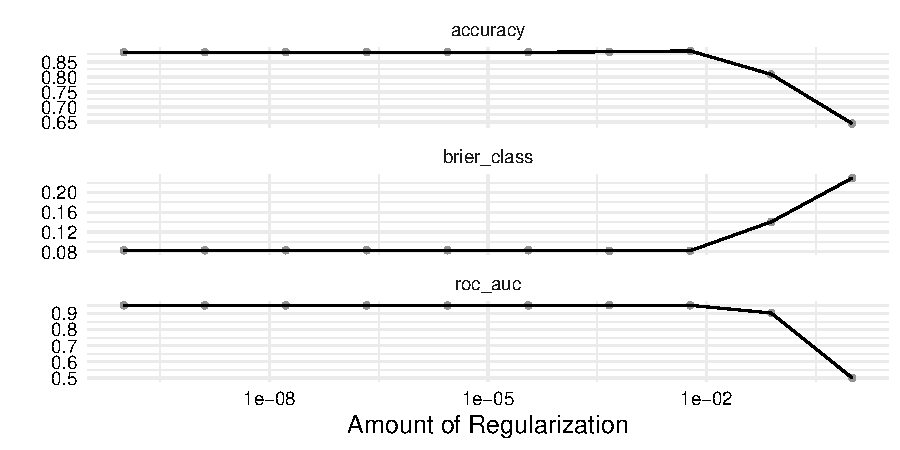
\includegraphics{part_4/9_predict_files/figure-pdf/fig-predict-class-model-spec-tune-grid-collect-1.pdf}

}

\caption{\label{fig-predict-class-model-spec-tune-grid-collect}Metrics
for each fold of the tuning process}

\end{figure}%

\end{minipage}%

\end{figure}%

\end{example}

The most common metrics for model performance in classification are
accuracy and the area under the \textbf{receiver operating
characteristic curve} (ROC-AUC). Accuracy is the proportion of correct
predictions. The ROC-AUC is a measure of how well the model can
distinguish between the two classes.

In the plot of the metrics, we can see that the many of the penalty
values performed similarly, with a drop off in performance at the higher
values. Conveniently, the \texttt{show\_best()} function from \{tune\}
takes a \texttt{tune\_grid} object and returns the best performing
hyperparameter values. The code is seen in
Example~\ref{exm-predict-class-model-spec-tune-grid-collect-best}.

\begin{example}[]\protect\hypertarget{exm-predict-class-model-spec-tune-grid-collect-best}{}\label{exm-predict-class-model-spec-tune-grid-collect-best}

~

\begin{Shaded}
\begin{Highlighting}[]
\CommentTok{\# Show the best performing hyperparameter value}
\NormalTok{cls\_tune }\SpecialCharTok{|\textgreater{}}
  \FunctionTok{show\_best}\NormalTok{(}\AttributeTok{metric =} \StringTok{"roc\_auc"}\NormalTok{)}
\end{Highlighting}
\end{Shaded}

\begin{verbatim}
# A tibble: 5 x 7
        penalty .metric .estimator  mean     n std_err .config              
          <dbl> <chr>   <chr>      <dbl> <int>   <dbl> <chr>                
1 0.000464      roc_auc binary     0.952    10 0.00487 Preprocessor1_Model07
2 0.00599       roc_auc binary     0.952    10 0.00344 Preprocessor1_Model08
3 0.0000000001  roc_auc binary     0.951    10 0.00502 Preprocessor1_Model01
4 0.00000000129 roc_auc binary     0.951    10 0.00502 Preprocessor1_Model02
5 0.0000000167  roc_auc binary     0.951    10 0.00502 Preprocessor1_Model03
\end{verbatim}

\end{example}

We can make this selection programmatically by using the
\texttt{select\_best()} function. This function needs a metric to select
by. We will use the ROC-AUC and select the best value for the penalty
hyperparameter. The code is seen in
Example~\ref{exm-predict-class-model-spec-tune-grid-collect-select}.

\begin{example}[]\protect\hypertarget{exm-predict-class-model-spec-tune-grid-collect-select}{}\label{exm-predict-class-model-spec-tune-grid-collect-select}

~

\begin{Shaded}
\begin{Highlighting}[]
\CommentTok{\# Select the best performing hyperparameter value}
\NormalTok{cls\_best }\OtherTok{\textless{}{-}}
  \FunctionTok{select\_best}\NormalTok{(cls\_tune, }\AttributeTok{metric =} \StringTok{"roc\_auc"}\NormalTok{)}

\CommentTok{\# Preview}
\NormalTok{cls\_best}
\end{Highlighting}
\end{Shaded}

\begin{verbatim}
# A tibble: 1 x 2
   penalty .config              
     <dbl> <chr>                
1 0.000464 Preprocessor1_Model07
\end{verbatim}

\end{example}

All of that to tune a hyperparameter!

Now we can update the model specification and workflow with the best
performing hyperparameter value using the previous
\texttt{cls\_wf\_tune} workflow and the \texttt{finalize\_workflow()}
function. The \texttt{finalize\_workflow()} function takes a workflow
and the selected parameters and returns an updated \texttt{workflow}
object, as seen in
Example~\ref{exm-predict-class-tune-hyperparameters-update-workflow}.

\begin{example}[]\protect\hypertarget{exm-predict-class-tune-hyperparameters-update-workflow}{}\label{exm-predict-class-tune-hyperparameters-update-workflow}

~

\begin{Shaded}
\begin{Highlighting}[]
\CommentTok{\# Update model specification}
\NormalTok{cls\_wf\_lasso }\OtherTok{\textless{}{-}}
\NormalTok{  cls\_wf }\SpecialCharTok{|\textgreater{}}
  \FunctionTok{finalize\_workflow}\NormalTok{(cls\_best)}

\CommentTok{\# Preview}
\NormalTok{cls\_wf\_lasso}
\end{Highlighting}
\end{Shaded}

\begin{Shaded}
\begin{Highlighting}[]
\NormalTok{══ Workflow ═══════════════════════════════════════}
\NormalTok{Preprocessor: Recipe}
\NormalTok{Model: logistic\_reg()}

\NormalTok{── Preprocessor ───────────────────────────────────}

\NormalTok{• step\_tokenize()}
\NormalTok{• step\_tokenfilter()}
\NormalTok{• step\_tfidf()}

\NormalTok{── Model ──────────────────────────────────────────}
\NormalTok{Logistic Regression Model Specification (classification)}

\NormalTok{Main Arguments:}
\NormalTok{  penalty = 0.000464158883361278}
\NormalTok{  mixture = 1}

\NormalTok{Computational engine: glmnet}
\end{Highlighting}
\end{Shaded}

\end{example}

Our model specification and the worflow are updated with the tuned
hyperparameter.

As a reminder we are still working in step 5 of our workflow,
interrogating the data. So far, we have selected and engineered the
features, split the data into training and testing sets, and selected a
classification algorithm. We have also tuned the hyperparameters of the
model and updated the model specification and workflow with the best
performing hyperparameter value.

The next step is to assess the performance of the model on the training
set given the features we have engineered, the algorithm we have
selected, and the hyperparameters we have tuned. Instead of evaluating
the model on the training set directly, we will use cross-validation on
the training set to gauge the variability of the model.

The reason for this is that the model's performance on the entire
training set at once is not a reliable indicator of the model's
performance on new data --just imagine if you were to take a test on the
same material over and over again, you would get better and better at
the test, but that doesn't mean you've learned the material any better.
Cross-validation is a technique that allows us to estimate the model's
performance on new data by simulating the process of training and
testing the model on different subsets of the training data.

Similar to what we did to tune the hyperparameters, we can use
cross-validation to gauge the variability of the model. The
\texttt{fit\_resamples()} function takes a workflow and a resampling
object and returns metrics for each fold. The code is seen in
Example~\ref{exm-predict-class-tune-hyperparameters-evaluate-workflow-cv}.

\begin{example}[]\protect\hypertarget{exm-predict-class-tune-hyperparameters-evaluate-workflow-cv}{}\label{exm-predict-class-tune-hyperparameters-evaluate-workflow-cv}

~

\begin{Shaded}
\begin{Highlighting}[]
\CommentTok{\# Cross{-}validate workflow}
\NormalTok{cls\_lasso\_cv }\OtherTok{\textless{}{-}}
\NormalTok{  cls\_wf\_lasso }\SpecialCharTok{|\textgreater{}}
  \FunctionTok{fit\_resamples}\NormalTok{(}
    \AttributeTok{resamples =}\NormalTok{ cls\_vfold,}
    \CommentTok{\# save predictions for confusion matrix}
    \AttributeTok{control =} \FunctionTok{control\_resamples}\NormalTok{(}\AttributeTok{save\_pred =} \ConstantTok{TRUE}\NormalTok{)}
\NormalTok{  )}
\end{Highlighting}
\end{Shaded}

\end{example}

We want to aggregate the metrics across the folds to get a sense of the
variability of the model. The \texttt{collect\_metrics()} function takes
the results of a cross-validation and returns a data frame with the
metrics.

\begin{example}[]\protect\hypertarget{exm-predict-class-tune-hyperparameters-evaluate-workflow-cv-collect}{}\label{exm-predict-class-tune-hyperparameters-evaluate-workflow-cv-collect}

~

\begin{Shaded}
\begin{Highlighting}[]
\CommentTok{\# Collect metrics}
\NormalTok{cls\_lasso\_cv }\SpecialCharTok{|\textgreater{}} \FunctionTok{collect\_metrics}\NormalTok{()}
\end{Highlighting}
\end{Shaded}

\begin{verbatim}
# A tibble: 2 x 6
  .metric  .estimator  mean     n std_err .config             
  <chr>    <chr>      <dbl> <int>   <dbl> <chr>               
1 accuracy binary     0.884    10 0.00554 Preprocessor1_Model1
2 roc_auc  binary     0.952    10 0.00487 Preprocessor1_Model1
\end{verbatim}

\end{example}

From the accuracy and ROC-AUC metrics in
Example~\ref{exm-predict-class-tune-hyperparameters-evaluate-workflow-cv-collect}
it appears we have a decent candidate model, but there is room for
potential improvement. A good next step is to evaluate the model errors
and see if there are any patterns that can be addressed before
considering what approach to take to improve the model.

\begin{tcolorbox}[enhanced jigsaw, left=2mm, toprule=.15mm, colback=white, colframe=quarto-callout-color-frame, arc=.35mm, rightrule=.15mm, bottomrule=.15mm, leftrule=.75mm, breakable, opacityback=0]

\textbf{\faIcon{hand-point-up} Tip}

To provide context in terms of what is a good model performance, it is
useful to compare the model's performance to a null model. A
\textbf{null model } (or baseline model) is a simple model that is easy
to implement and provides a benchmark for the model's performance. For
classification tasks, a common null model is to predict the most
frequent class. In modeling, this is the minimal benchmark we want to
beat, if we are doing better than this, we are doing better than chance.

\end{tcolorbox}

For classification tasks, a good place to start is to visualize a
confusion matrix. A \textbf{confusion matrix} is a cross-tabulation of
the predicted and actual outcomes. The \texttt{conf\_mat\_resampled()}
function takes a \texttt{fit\_resamples} object (with predictions saved)
and returns a table (\texttt{tidy\ =\ FALSE}) with the confusion matrix
for the aggregated folds. We can pass this to the \texttt{autoplot()}
function to plot as in
Example~\ref{exm-predict-class-tune-hyperparameters-evaluate-workflow-cv-confusion}.

\begin{example}[]\protect\hypertarget{exm-predict-class-tune-hyperparameters-evaluate-workflow-cv-confusion}{}\label{exm-predict-class-tune-hyperparameters-evaluate-workflow-cv-confusion}

~

\begin{Shaded}
\begin{Highlighting}[]
\CommentTok{\# Plot confusion matrix}
\NormalTok{cls\_lasso\_cv }\SpecialCharTok{|\textgreater{}}
  \FunctionTok{conf\_mat\_resampled}\NormalTok{(}\AttributeTok{tidy =} \ConstantTok{FALSE}\NormalTok{) }\SpecialCharTok{|\textgreater{}}
  \FunctionTok{autoplot}\NormalTok{(}\AttributeTok{type =} \StringTok{"heatmap"}\NormalTok{)}
\end{Highlighting}
\end{Shaded}

\begin{figure}[!htb]

\centering{

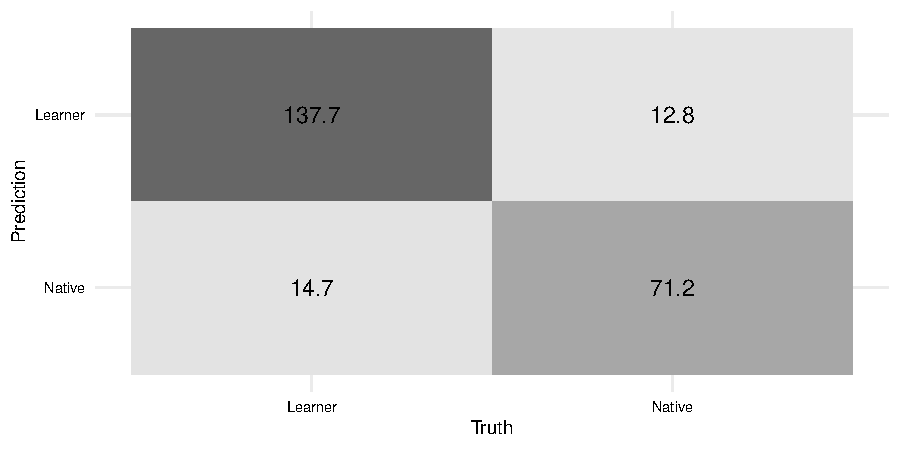
\includegraphics{part_4/9_predict_files/figure-pdf/fig-class-tune-hyperparameters-evaluate-workflow-cv-confusion-1.pdf}

}

\caption{\label{fig-class-tune-hyperparameters-evaluate-workflow-cv-confusion}Confusion
matrix for the aggregated folds of the cross-validation}

\end{figure}%

\end{example}

The top left to bottom right diagonal contains the true positives and
true negatives, these are the correct predictions. The top right to
bottom left diagonal contains the false positives and false negatives
--our errors. The convention is speak of one class being the positive
class and the other class being the negative class. In our case, we will
consider the positive class to be the `learner' class and the negative
class to be the `natives' class.

We can see that there are more learners falsely predicted to be natives
than the other way around. This may be due to the fact that there are
simply more learners than natives in the data set or this could signal
that there are some learners that are more similar to natives than other
learners. Clearly this can't be the entire explanation as the model is
not perfect, even some natives are classified falsely as learners! But
may be an interesting avenue for further exploration. Maybe these are
learners that are more advanced or have a particular style of writing
that is more similar to natives.

\begin{tcolorbox}[enhanced jigsaw, left=2mm, toprule=.15mm, colback=white, colframe=quarto-callout-color-frame, arc=.35mm, rightrule=.15mm, bottomrule=.15mm, leftrule=.75mm, breakable, opacityback=0]

\textbf{\faIcon{medal} Dive deeper}

Another perspective often applied to evaluate a model is the Reciever
Operating Characteristic (ROC) curve. The ROC curve is a plot of the
true positive rate (TPR) against the false positive rate (FPR) for
different classification thresholds. This metric, and visualization, can
be useful to gauge the model's ability to distinguish between the two
classes. \{yardstick\} provides the \texttt{roc\_curve()} function to
calculate the ROC curve on a \texttt{fit\_resamples} object.

\end{tcolorbox}

To improve supervised learning models, one should consider a number of
possibilities:

\begin{enumerate}
\def\labelenumi{\arabic{enumi}.}
\tightlist
\item
  Engineer the features differently
\item
  Select different (or additional) features
\item
  Change the algorithm
\item
  Tune the hyperparameters differently
\end{enumerate}

Of these options, adjusting the feature engineering features process is
the option that diverges least from our current workflow
\texttt{cls\_wf\_lasso}. Recall that in our recipe specification we set
a token filter to limit the number of features to 100. We can adjust
this number to see if it has an effect on the model's performance.

To avoid help select the optimimal number of tokens, we again can use
the tuning process we explored for the hyperparameters. This time,
however, the \texttt{tune()} placeholder will be included as the
argument to the \texttt{max\_tokens} argument in the
\texttt{step\_tokenfilter()} function.

I repeat the recipe with the tuning placeholder in
Example~\ref{exm-predict-class-tune-hyperparameters-tokenfilter}.

\begin{example}[]\protect\hypertarget{exm-predict-class-tune-hyperparameters-tokenfilter}{}\label{exm-predict-class-tune-hyperparameters-tokenfilter}

~

\begin{Shaded}
\begin{Highlighting}[]
\CommentTok{\# Create a recipe with a token filter step}
\NormalTok{cls\_rec }\OtherTok{\textless{}{-}}
  \FunctionTok{recipe}\NormalTok{(}
    \AttributeTok{formula =}\NormalTok{ outcome }\SpecialCharTok{\textasciitilde{}}\NormalTok{ text,}
    \AttributeTok{data =}\NormalTok{ cls\_train}
\NormalTok{    ) }\SpecialCharTok{|\textgreater{}}
  \FunctionTok{step\_tokenize}\NormalTok{(text) }\SpecialCharTok{|\textgreater{}}
  \FunctionTok{step\_tokenfilter}\NormalTok{(text, }\AttributeTok{max\_tokens =} \FunctionTok{tune}\NormalTok{()) }\SpecialCharTok{|\textgreater{}}
  \FunctionTok{step\_tfidf}\NormalTok{(text)}
\end{Highlighting}
\end{Shaded}

\end{example}

With the updated recipe, we can update the \texttt{cls\_wf\_lasso} and
tune the \texttt{max\_tokens} hyperparameter. The code is seen in
Example~\ref{exm-predict-class-tune-hyperparameters-update-rec}.

\begin{example}[]\protect\hypertarget{exm-predict-class-tune-hyperparameters-update-rec}{}\label{exm-predict-class-tune-hyperparameters-update-rec}

~

\begin{Shaded}
\begin{Highlighting}[]
\CommentTok{\# Update workflow with token filter tuning}
\NormalTok{cls\_wf\_lasso }\OtherTok{\textless{}{-}}
\NormalTok{  cls\_wf\_lasso }\SpecialCharTok{|\textgreater{}}
  \FunctionTok{update\_recipe}\NormalTok{(cls\_rec)}
\end{Highlighting}
\end{Shaded}

\end{example}

One thing to note is that we will want to consider what values of
\texttt{max\_tokens} we want to use to tune the hyperparameter. So
instead of only specifying the levels in the \texttt{grid\_regular()}
function, we are best off to provide a range of values that we think are
reasonable. Let's add a range of values between our current value 100
and 2,000 to start. And let's tell the grid to select five values from
this range.

The code is seen in
Example~\ref{exm-predict-class-tune-hyperparameters-tokenfilter-grid}.

\begin{example}[]\protect\hypertarget{exm-predict-class-tune-hyperparameters-tokenfilter-grid}{}\label{exm-predict-class-tune-hyperparameters-tokenfilter-grid}

~

\begin{Shaded}
\begin{Highlighting}[]
\CommentTok{\# Create a grid of values for the max tokens hyperparameter}
\NormalTok{cls\_grid }\OtherTok{\textless{}{-}}
  \FunctionTok{grid\_regular}\NormalTok{(}\FunctionTok{max\_tokens}\NormalTok{(}\AttributeTok{range =} \FunctionTok{c}\NormalTok{(}\DecValTok{100}\NormalTok{, }\DecValTok{2000}\NormalTok{)), }\AttributeTok{levels =} \DecValTok{5}\NormalTok{)}

\CommentTok{\# Preview}
\NormalTok{cls\_grid}
\end{Highlighting}
\end{Shaded}

\begin{verbatim}
# A tibble: 5 x 1
  max_tokens
       <int>
1        100
2        575
3       1050
4       1525
5       2000
\end{verbatim}

\end{example}

From here, the process is the same as before. We will use the
\texttt{tune\_grid()} function to tune the \texttt{max\_tokens}
hyperparameter, select the best value, and finalize the workflow, as
seen from Example~\ref{exm-predict-class-model-spec-tune-grid-cv}
through
Example~\ref{exm-predict-class-tune-hyperparameters-update-workflow}.

After tuning the \texttt{max\_tokens} hyperparameter, the best
performing value is 1,050. We now used the updated
\texttt{cls\_wf\_lasso\_tokens} workflow to cross-validate the model and
collect the metrics. The code is seen in
Example~\ref{exm-predict-class-tune-hyperparameters-tokenfilter-evaluate-workflow-cv-collect}.

\begin{example}[]\protect\hypertarget{exm-predict-class-tune-hyperparameters-tokenfilter-evaluate-workflow-cv-collect}{}\label{exm-predict-class-tune-hyperparameters-tokenfilter-evaluate-workflow-cv-collect}

~

\begin{Shaded}
\begin{Highlighting}[]
\CommentTok{\# Cross{-}validate workflow}
\NormalTok{cls\_lasso\_tokens\_cv }\OtherTok{\textless{}{-}}
\NormalTok{  cls\_wf\_lasso\_tokens }\SpecialCharTok{|\textgreater{}}
  \FunctionTok{fit\_resamples}\NormalTok{(}
    \AttributeTok{resamples =}\NormalTok{ cls\_vfold,}
    \CommentTok{\# save predictions for confusion matrix}
    \AttributeTok{control =} \FunctionTok{control\_resamples}\NormalTok{(}\AttributeTok{save\_pred =} \ConstantTok{TRUE}\NormalTok{)}
\NormalTok{  )}

\CommentTok{\# Collect metrics}
\NormalTok{cls\_lasso\_tokens\_cv }\SpecialCharTok{|\textgreater{}}
  \FunctionTok{collect\_metrics}\NormalTok{()}
\end{Highlighting}
\end{Shaded}

\begin{verbatim}
# A tibble: 2 x 6
  .metric  .estimator  mean     n std_err .config             
  <chr>    <chr>      <dbl> <int>   <dbl> <chr>               
1 accuracy binary     0.918    10 0.00555 Preprocessor1_Model1
2 roc_auc  binary     0.968    10 0.00289 Preprocessor1_Model1
\end{verbatim}

\end{example}

The metrics from
Example~\ref{exm-predict-class-tune-hyperparameters-tokenfilter-evaluate-workflow-cv-collect}
show that the model's performance has improved for both the accuracy and
the ROC-AUC. The confusion matrix from
Example~\ref{exm-predict-class-tune-hyperparameters-tokenfilter-evaluate-workflow-cv-confusion}
shows that the number of false positives and false negatives has
decreased. This is a good sign that the model is more robust.

\begin{example}[]\protect\hypertarget{exm-predict-class-tune-hyperparameters-tokenfilter-evaluate-workflow-cv-confusion}{}\label{exm-predict-class-tune-hyperparameters-tokenfilter-evaluate-workflow-cv-confusion}

~

\begin{Shaded}
\begin{Highlighting}[]
\CommentTok{\# Plot confusion matrix}
\NormalTok{cls\_lasso\_tokens\_cv }\SpecialCharTok{|\textgreater{}}
  \FunctionTok{conf\_mat\_resampled}\NormalTok{(}\AttributeTok{tidy =} \ConstantTok{FALSE}\NormalTok{) }\SpecialCharTok{|\textgreater{}}
  \FunctionTok{autoplot}\NormalTok{(}\AttributeTok{type =} \StringTok{"heatmap"}\NormalTok{)}
\end{Highlighting}
\end{Shaded}

\begin{figure}[!htb]

\centering{

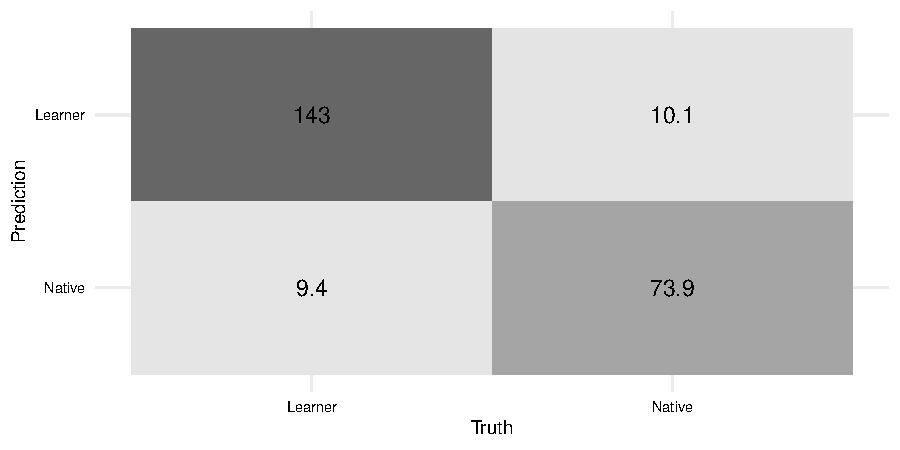
\includegraphics{part_4/9_predict_files/figure-pdf/fig-predict-class-tune-hyperparameters-tokenfilter-evaluate-workflow-cv-confusion-1.pdf}

}

\caption{\label{fig-predict-class-tune-hyperparameters-tokenfilter-evaluate-workflow-cv-confusion}Confusion
matrix for the aggregated folds of the cross-validation}

\end{figure}%

\end{example}

It appears that the model is more robust with the updated
\texttt{max\_tokens} hyperparameter. We could continue to explore other
model improvement strategies, but for now we will move on to the next
step in our workflow.

We are now ready to move on to step 7, evaluating the model on the test
set. To do this we need to fit the tuned workflow to the training set,
which is the actual training phase. We will use the \texttt{last\_fit()}
function from \{workflows\} to fit the workflow to the training set.

The \texttt{last\_fit()} function takes a workflow and a split object
and returns a \texttt{last\_fit} object. The \texttt{last\_fit} object
contains the results of the model fit on the training set and the
results of the model evaluation on the test set. The code is seen in
Example~\ref{exm-predict-class-tune-hyperparameters-evaluate-test}.

We will use the \texttt{last\_fit()} function to train the final model
and predict the outcome on the test set. The \texttt{collect\_metrics()}
function takes a data frame with the actual and predicted outcomes and
returns a data frame with the metrics for the model. The code is seen in
Example~\ref{exm-predict-class-tune-hyperparameters-evaluate-test}.

\begin{example}[]\protect\hypertarget{exm-predict-class-tune-hyperparameters-evaluate-test}{}\label{exm-predict-class-tune-hyperparameters-evaluate-test}

~

\begin{Shaded}
\begin{Highlighting}[]
\CommentTok{\# Fit the model to the training set and}
\CommentTok{\# evaluate on the test set}
\NormalTok{cls\_final\_fit }\OtherTok{\textless{}{-}}
  \FunctionTok{last\_fit}\NormalTok{(}
\NormalTok{    cls\_wf\_lasso\_tokens,}
    \AttributeTok{split =}\NormalTok{ cls\_split}
\NormalTok{  )}

\CommentTok{\# Evaluate model on testing set}
\NormalTok{cls\_final\_fit }\SpecialCharTok{|\textgreater{}}
  \FunctionTok{collect\_metrics}\NormalTok{()}
\end{Highlighting}
\end{Shaded}

\begin{verbatim}
# A tibble: 2 x 4
  .metric  .estimator .estimate .config             
  <chr>    <chr>          <dbl> <chr>               
1 accuracy binary         0.909 Preprocessor1_Model1
2 roc_auc  binary         0.962 Preprocessor1_Model1
\end{verbatim}

\end{example}

The performance metrics are very close to those we achieved on the
training set in
Example~\ref{exm-predict-class-tune-hyperparameters-tokenfilter-evaluate-workflow-cv-collect}.
This is a good sign that the model is robust as it performs well on both
training and test sets. We can evaluate the confusion matrix on the test
set as well. The code is seen in
Example~\ref{exm-predict-class-tune-hyperparameters-evaluate-test-confusion}.

\begin{example}[]\protect\hypertarget{exm-predict-class-tune-hyperparameters-evaluate-test-confusion}{}\label{exm-predict-class-tune-hyperparameters-evaluate-test-confusion}

~

\begin{Shaded}
\begin{Highlighting}[]
\CommentTok{\# Plot confusion matrix}
\NormalTok{cls\_final\_fit }\SpecialCharTok{|\textgreater{}}
  \FunctionTok{collect\_predictions}\NormalTok{() }\SpecialCharTok{|\textgreater{}}
  \FunctionTok{conf\_mat}\NormalTok{(}\AttributeTok{truth =}\NormalTok{ outcome, }\AttributeTok{estimate =}\NormalTok{ .pred\_class) }\SpecialCharTok{|\textgreater{}}
  \FunctionTok{autoplot}\NormalTok{(}\AttributeTok{type =} \StringTok{"heatmap"}\NormalTok{)}
\end{Highlighting}
\end{Shaded}

\begin{figure}[!htb]

\centering{

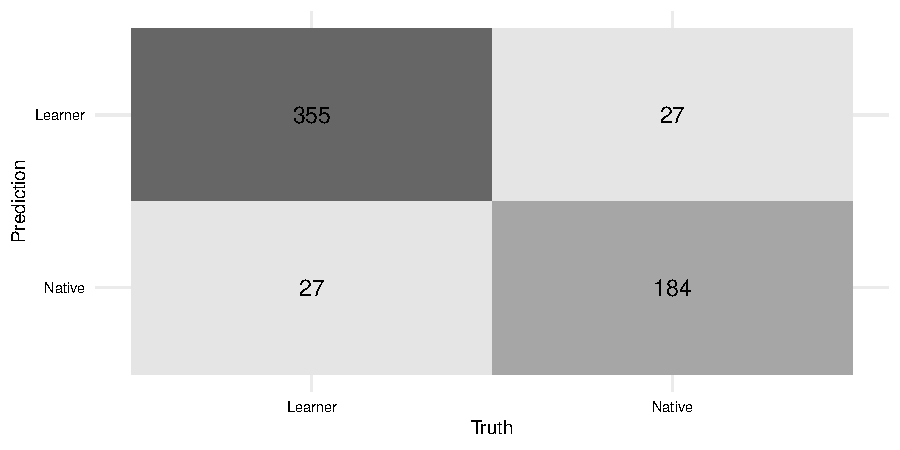
\includegraphics{part_4/9_predict_files/figure-pdf/fig-predict-class-tune-hyperparameters-evaluate-test-confusion-1.pdf}

}

\caption{\label{fig-predict-class-tune-hyperparameters-evaluate-test-confusion}Confusion
matrix for the test set}

\end{figure}%

\end{example}

On the test set the false instances are balanced, which is a good sign
that the model is robust. Ideally, there would be no errors, but this is
not realistic. The model is not perfect, but it is useful.

Now a model that can predict the nativeness of a writer based on their
writing sample is a useful tool in itself. You could imagine that this
could be a preprocessing step for a language learning application, for
example. But for a study that is more interested in learning about what
features are most important for predicting the native versus non-native
features of a writer, we still have some work to do. We can inspect the
errors on the test set to gain some insight into what writing samples,
and which proficiency levels of the writers, are most difficult to
predict. We can also inspect the estimates for the features in the model
to gain some insight into what features are most important for
predicting the outcomes.

Let's first approach this from a document-proficiency point of view.
First, we will want to integrate the predictions with the test set to
inspect the errors. We can use the \texttt{collect\_predictions()}
function to collect the predictions from the \texttt{last\_fit} object
and attach them with the test set \texttt{cls\_test} with
\texttt{bind\_cols}. Note, we can drop the \texttt{outcome} variable
from \texttt{cls\_test} as we have this column in our fitted model. The
code is seen in
Example~\ref{exm-predict-class-tune-hyperparameters-integrate-test}.

\begin{example}[]\protect\hypertarget{exm-predict-class-tune-hyperparameters-integrate-test}{}\label{exm-predict-class-tune-hyperparameters-integrate-test}

~

\begin{Shaded}
\begin{Highlighting}[]
\CommentTok{\# Collect predictions from the model}
\NormalTok{cls\_lasso\_fit\_preds\_test }\OtherTok{\textless{}{-}}
\NormalTok{  cls\_final\_fit }\SpecialCharTok{|\textgreater{}}
  \FunctionTok{collect\_predictions}\NormalTok{() }\SpecialCharTok{|\textgreater{}}
  \FunctionTok{bind\_cols}\NormalTok{(cls\_test[, }\SpecialCharTok{{-}}\DecValTok{1}\NormalTok{])}

\CommentTok{\# Preview}
\FunctionTok{glimpse}\NormalTok{(cls\_lasso\_fit\_preds\_test)}
\end{Highlighting}
\end{Shaded}

\begin{verbatim}
Rows: 593
Columns: 9
$ id            <chr> "train/test split", "train/test split", "train/test spli~
$ .pred_Learner <dbl> 1.0000, 1.0000, 1.0000, 0.0996, 1.0000, 0.9928, 1.0000, ~
$ .pred_Native  <dbl> 9.59e-06, 1.13e-05, 3.16e-09, 9.00e-01, 2.83e-06, 7.17e-~
$ .row          <int> 3, 7, 15, 21, 22, 25, 36, 43, 47, 50, 53, 57, 62, 66, 68~
$ .pred_class   <fct> Learner, Learner, Learner, Native, Learner, Learner, Lea~
$ outcome       <fct> Learner, Learner, Learner, Learner, Learner, Learner, Le~
$ .config       <chr> "Preprocessor1_Model1", "Preprocessor1_Model1", "Preproc~
$ proficiency   <fct> Lower beginner, Lower beginner, Lower beginner, Lower be~
$ text          <chr> "Sanaa Lathan es muy famosa persona. Ella es en de telev~
\end{verbatim}

\end{example}

I will then select the columns with the actual outcome, the predicted
outcome, the proficiency level, and the text and separate the predicted
outcome to inspect them separately, as seen in
Example~\ref{exm-predict-class-tune-hyperparameters-evaluate-test-errors}.

\begin{example}[]\protect\hypertarget{exm-predict-class-tune-hyperparameters-evaluate-test-errors}{}\label{exm-predict-class-tune-hyperparameters-evaluate-test-errors}

~

\begin{Shaded}
\begin{Highlighting}[]
\CommentTok{\# Inspect errors}
\NormalTok{cls\_lasso\_fit\_preds\_test }\SpecialCharTok{|\textgreater{}}
  \FunctionTok{filter}\NormalTok{(outcome }\SpecialCharTok{!=}\NormalTok{ .pred\_class) }\SpecialCharTok{|\textgreater{}}
  \FunctionTok{select}\NormalTok{(outcome, .pred\_class, proficiency, text)}
\end{Highlighting}
\end{Shaded}

\begin{verbatim}
# A tibble: 54 x 4
   outcome .pred_class proficiency        text                                  
   <fct>   <fct>       <fct>              <chr>                                 
 1 Learner Native      Lower beginner     "Un día un pequeño nino fue dado una ~
 2 Learner Native      Upper beginner     "Un dia, El niño estaba durmiendo cua~
 3 Learner Native      Upper beginner     "Yo vivo en la ciudad de Atlanta. En ~
 4 Learner Native      Upper beginner     "Hola me llamo Jason.\n Mis amigos es~
 5 Learner Native      Lower intermediate "Recientemente vi una película que es~
 6 Learner Native      Upper intermediate "Vivo en la ciudad de Richmond en Vir~
 7 Learner Native      Upper intermediate "A la semana pasada, yo vi la pelicul~
 8 Learner Native      Upper intermediate "Un día decidí llevarme a casa una ra~
 9 Learner Native      Lower advanced     "Bueno, el año pasado mi novia y yo v~
10 Learner Native      Lower advanced     "Un día Pablo, un niño de 6 años, enc~
# i 44 more rows
\end{verbatim}

\begin{Shaded}
\begin{Highlighting}[]
\CommentTok{\# Inspect learners falsely predicted to be natives}
\NormalTok{cls\_lasso\_fit\_preds\_test }\SpecialCharTok{|\textgreater{}}
  \FunctionTok{filter}\NormalTok{(outcome }\SpecialCharTok{==} \StringTok{"Learner"}\NormalTok{, .pred\_class }\SpecialCharTok{==} \StringTok{"Native"}\NormalTok{) }\SpecialCharTok{|\textgreater{}}
  \FunctionTok{select}\NormalTok{(outcome, .pred\_class, proficiency, text) }\SpecialCharTok{|\textgreater{}}
  \FunctionTok{count}\NormalTok{(proficiency, }\AttributeTok{sort =} \ConstantTok{TRUE}\NormalTok{)}
\end{Highlighting}
\end{Shaded}

\begin{verbatim}
# A tibble: 6 x 2
  proficiency            n
  <fct>              <int>
1 Upper advanced        10
2 Lower advanced         9
3 Upper beginner         3
4 Upper intermediate     3
5 Lower beginner         1
6 Lower intermediate     1
\end{verbatim}

\end{example}

Interestingly, the majority of misclassified learners are advanced,
which could be expected as they are more similar to natives. There are
some beginners that are misclassified as natives, but this is not as
common. Yes, it is still an open question as to why some natives are
classified as learners.

We can inspect the estimates for the features in the model to gain some
insight into what features are most important for predicting the
outcomes. The \texttt{extract\_fit\_parsnip()} function takes a trained
model specification \texttt{cls\_final\_fit} and returns a data frame
with the estimated coefficients for each feature. The code is seen in
Example~\ref{exm-predict-class-tune-hyperparameters-evaluate-test-estimates}.

\begin{example}[]\protect\hypertarget{exm-predict-class-tune-hyperparameters-evaluate-test-estimates}{}\label{exm-predict-class-tune-hyperparameters-evaluate-test-estimates}

~

\begin{Shaded}
\begin{Highlighting}[]
\CommentTok{\# Extract estimates}
\NormalTok{cls\_final\_fit\_features }\OtherTok{\textless{}{-}}
\NormalTok{  cls\_final\_fit }\SpecialCharTok{|\textgreater{}}
  \FunctionTok{extract\_fit\_parsnip}\NormalTok{() }\SpecialCharTok{|\textgreater{}}
  \FunctionTok{tidy}\NormalTok{()}
\end{Highlighting}
\end{Shaded}

\end{example}

The estimates are the log odds of the outcome. In a binary
classification task, the log odds of the outcome is the log of the
probability of the outcome divided by the probability of the other
outcome. In our case, the reference outcome is ``Learner'', so negative
log-odds indicate that the feature is associated with the ``Learner''
outcome and positive log-odds indicate that the feature is associated
with the ``Native'' outcome.

The estimates are in log-odds, so we need to exponentiate them to get
the odds. The odds are the probability of the outcome divided by the
probability of the other outcome. The probability of the outcome is the
odds divided by the odds plus one. The code is seen in
Example~\ref{exm-predict-class-tune-hyperparameters-evaluate-test-estimates-probability}.

\begin{example}[]\protect\hypertarget{exm-predict-class-tune-hyperparameters-evaluate-test-estimates-probability}{}\label{exm-predict-class-tune-hyperparameters-evaluate-test-estimates-probability}

~

\begin{Shaded}
\begin{Highlighting}[]
\CommentTok{\# Calculate probability}
\NormalTok{cls\_final\_fit\_features }\SpecialCharTok{|\textgreater{}}
  \FunctionTok{mutate}\NormalTok{(}\AttributeTok{probability =} \FunctionTok{exp}\NormalTok{(estimate) }\SpecialCharTok{/}\NormalTok{ (}\FunctionTok{exp}\NormalTok{(estimate) }\SpecialCharTok{+} \DecValTok{1}\NormalTok{))}
\end{Highlighting}
\end{Shaded}

\begin{verbatim}
# A tibble: 1,051 x 4
   term                  estimate  penalty probability
   <chr>                    <dbl>    <dbl>       <dbl>
 1 (Intercept)             -13.6  0.000464  0.00000129
 2 tfidf_text_10             0    0.000464  0.5       
 3 tfidf_text_2              0    0.000464  0.5       
 4 tfidf_text_3              0    0.000464  0.5       
 5 tfidf_text_4              0    0.000464  0.5       
 6 tfidf_text_5              0    0.000464  0.5       
 7 tfidf_text_a             64.9  0.000464  1         
 8 tfidf_text_abandonado     7.02 0.000464  0.999     
 9 tfidf_text_abuela        -8.64 0.000464  0.000176  
10 tfidf_text_abuelos        2.14 0.000464  0.895     
# i 1,041 more rows
\end{verbatim}

\end{example}

So just looking at the snippet of the features returned from
Example~\ref{exm-predict-class-tune-hyperparameters-evaluate-test-estimates-probability},
we can see that the features `a' and `abandonado' are associated with
the ``Native'' outcome, `abuela' is associated with ``Learners'', and
the other features are neutral (\texttt{probability} = 0.5).

A quick way to extract the most important features for predicting the
each outcome is to use the \texttt{vi()} function from \{vip\}. It takes
a trained model specification and returns a data frame with the most
important features. The code is seen in
Example~\ref{exm-predict-class-tune-hyperparameters-evaluate-test-vip}.

\begin{example}[]\protect\hypertarget{exm-predict-class-tune-hyperparameters-evaluate-test-vip}{}\label{exm-predict-class-tune-hyperparameters-evaluate-test-vip}

~

\begin{Shaded}
\begin{Highlighting}[]
\CommentTok{\# Load package}
\FunctionTok{library}\NormalTok{(vip)}

\CommentTok{\# Avoid conflicts for function names from other packages}
\NormalTok{conflicted}\SpecialCharTok{::}\FunctionTok{conflicts\_prefer}\NormalTok{(vip}\SpecialCharTok{::}\NormalTok{vi)}

\CommentTok{\# Extract important features}
\NormalTok{var\_importance\_tbl }\OtherTok{\textless{}{-}}
\NormalTok{  cls\_final\_fit }\SpecialCharTok{|\textgreater{}}
  \FunctionTok{extract\_fit\_parsnip}\NormalTok{() }\SpecialCharTok{|\textgreater{}}
  \FunctionTok{vi}\NormalTok{()}

\CommentTok{\# Preview}
\NormalTok{var\_importance\_tbl}
\end{Highlighting}
\end{Shaded}

\begin{verbatim}
# A tibble: 1,050 x 3
   Variable           Importance Sign 
   <chr>                   <dbl> <chr>
 1 tfidf_text_época         354. POS  
 2 tfidf_text_mayoría       320. NEG  
 3 tfidf_text_ésta          312. POS  
 4 tfidf_text_ante          278. POS  
 5 tfidf_text_proximo       274. NEG  
 6 tfidf_text_esperar       245. NEG  
 7 tfidf_text_mucha         244. NEG  
 8 tfidf_text_seguir        242. POS  
 9 tfidf_text_poder         241. POS  
10 tfidf_text_ahí           235. POS  
# i 1,040 more rows
\end{verbatim}

\end{example}

The \texttt{Variable} column contains each feature (with the feature
type and corresponding variable \texttt{tfidf\_text\_}),
\texttt{Importance} provides the absolute log-odds value, and the
\texttt{Sign} column indicates whether the feature is associated with
the ``NEG'' (``Learner'') or the ``POS'' (``Native'') outcome. We can
recode the \texttt{Variable} and \texttt{Sign} columns to make them more
interpretable and then plot them using \texttt{ggplot()}, as in
Example~\ref{exm-predict-class-tune-hyperparameters-evaluate-test-vip-plot}.

\begin{example}[]\protect\hypertarget{exm-predict-class-tune-hyperparameters-evaluate-test-vip-plot}{}\label{exm-predict-class-tune-hyperparameters-evaluate-test-vip-plot}

~

\begin{Shaded}
\begin{Highlighting}[]
\CommentTok{\# Recode variable and sign}
\NormalTok{var\_importance\_tbl }\OtherTok{\textless{}{-}}
\NormalTok{  var\_importance\_tbl }\SpecialCharTok{|\textgreater{}}
  \FunctionTok{mutate}\NormalTok{(}
    \AttributeTok{Feature =} \FunctionTok{str\_remove}\NormalTok{(Variable, }\StringTok{"tfidf\_text\_"}\NormalTok{),}
    \AttributeTok{Outcome =} \FunctionTok{case\_when}\NormalTok{(}
\NormalTok{      Sign }\SpecialCharTok{==} \StringTok{"NEG"} \SpecialCharTok{\textasciitilde{}} \StringTok{"Learner"}\NormalTok{,}
\NormalTok{      Sign }\SpecialCharTok{==} \StringTok{"POS"} \SpecialCharTok{\textasciitilde{}} \StringTok{"Native"}\NormalTok{),}
\NormalTok{    ) }\SpecialCharTok{|\textgreater{}}
  \FunctionTok{select}\NormalTok{(Outcome, Feature, Importance)}

\CommentTok{\# Plot}
\NormalTok{var\_importance\_tbl }\SpecialCharTok{|\textgreater{}}
  \FunctionTok{slice\_max}\NormalTok{(Importance, }\AttributeTok{n =} \DecValTok{50}\NormalTok{) }\SpecialCharTok{|\textgreater{}}
  \FunctionTok{ggplot}\NormalTok{(}\FunctionTok{aes}\NormalTok{(}\AttributeTok{x =} \FunctionTok{reorder}\NormalTok{(Feature, Importance), }\AttributeTok{y =}\NormalTok{ Importance)) }\SpecialCharTok{+}
  \FunctionTok{geom\_point}\NormalTok{() }\SpecialCharTok{+}
  \FunctionTok{coord\_flip}\NormalTok{() }\SpecialCharTok{+}
  \FunctionTok{facet\_wrap}\NormalTok{(}\SpecialCharTok{\textasciitilde{}}\NormalTok{ Outcome, }\AttributeTok{scales =} \StringTok{"free\_y"}\NormalTok{) }\SpecialCharTok{+}
  \FunctionTok{labs}\NormalTok{(}\AttributeTok{x =} \ConstantTok{NULL}\NormalTok{, }\AttributeTok{y =} \StringTok{"Importance"}\NormalTok{, }\AttributeTok{fill =} \ConstantTok{NULL}\NormalTok{) }\SpecialCharTok{+}
  \FunctionTok{theme\_minimal}\NormalTok{()}
\end{Highlighting}
\end{Shaded}

\begin{figure}[!htb]

\centering{

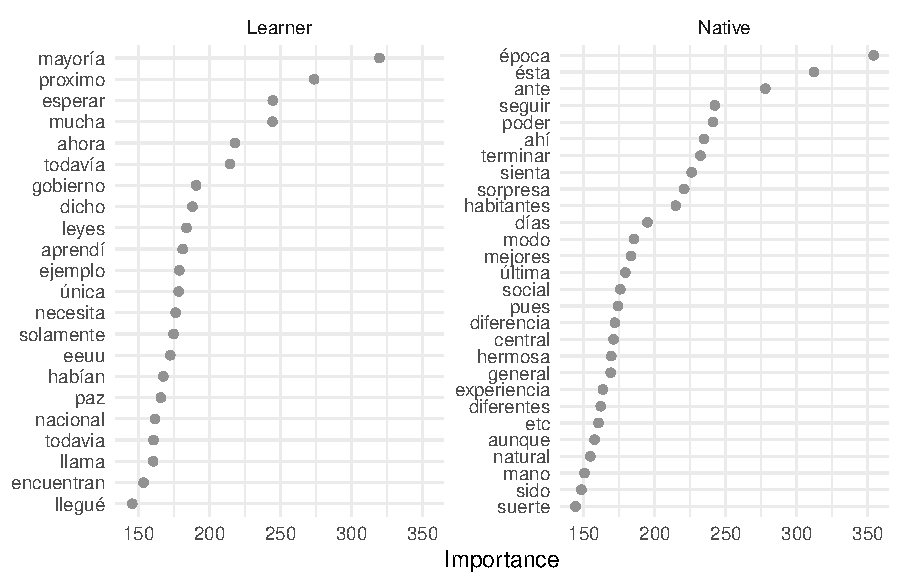
\includegraphics{part_4/9_predict_files/figure-pdf/fig-predict-class-tune-hyperparameters-evaluate-test-vip-plot-1.pdf}

}

\caption{\label{fig-predict-class-tune-hyperparameters-evaluate-test-vip-plot}Most
important features for predicting the outcome}

\end{figure}%

\end{example}

We can inspect
Figure~\ref{fig-predict-class-tune-hyperparameters-evaluate-test-vip-plot},
and qualitatively assess what these features may be telling us about the
differences between the learners and the natives.

In this section, we've build a text classifier using a regularized
logistic regression model. We've tuned the hyperparameters to arrive at
a robust model that performs well on both the training and test sets.
We've also evaluated the model errors and inspected the most important
features for predicting the outcome.

\subsection{Text regression}\label{sec-predict-text-regression}

We will now turn our attention to the second task in this section, text
regression. In this task, we will use the same original dataset as in
the classification task, but we will predict the placement score based
on the learner writing samples. I will make reference to but not repeat
the steps we took in the classification task, as many of the steps are
the same. This is one of the benefits of using tidymodels--the workflow
is by-and-large the same for different tasks.

Let's start by extracting the observations (only learners) and the
relevant variables from the original data set. The code is seen in
Example~\ref{exm-predict-reg-data}.

\begin{example}[]\protect\hypertarget{exm-predict-reg-data}{}\label{exm-predict-reg-data}

~

\begin{Shaded}
\begin{Highlighting}[]
\CommentTok{\# Extract observations and relevant variables}
\NormalTok{reg\_tbl }\OtherTok{\textless{}{-}}
\NormalTok{  cedel\_tbl }\SpecialCharTok{|\textgreater{}}
  \FunctionTok{filter}\NormalTok{(subcorpus }\SpecialCharTok{==} \StringTok{"Learner"}\NormalTok{) }\SpecialCharTok{|\textgreater{}}
  \FunctionTok{select}\NormalTok{(}\AttributeTok{outcome =}\NormalTok{ placement\_score, proficiency, text)}

\CommentTok{\# Preview}
\NormalTok{reg\_tbl }\SpecialCharTok{|\textgreater{}} \FunctionTok{glimpse}\NormalTok{()}
\end{Highlighting}
\end{Shaded}

\begin{verbatim}
Rows: 1,906
Columns: 3
$ outcome     <dbl> 14.0, 16.3, 16.3, 18.6, 18.6, 18.6, 20.9, 20.9, 20.9, 20.9~
$ proficiency <fct> Lower beginner, Lower beginner, Lower beginner, Lower begi~
$ text        <chr> "Yo vivo es Alanta, Georgia. Atlanta es muy grande ciudad.~
\end{verbatim}

\end{example}

In this task, our outcome variable is numeric and our predictor variable
\texttt{text} is the same as before. It might be useful to engineer the
features differently, but we will start with the same feature
engineering process as before, namely the \(tf\)-\(idf\) method for the
top 1,050 words.

I create a data split, \texttt{reg\_split} and the training and testing
sets, \texttt{reg\_train} and \texttt{reg\_test} and create a
\texttt{reg\_rec} recipe object which contains the starting recipe for
the regression task. And, since we are using the same recipe as before,
there is no need to validate the recipe. We can skip straight to the
model building.

As before we will want to start with a simple model and then build up to
more complex models. The list in
Table~\ref{tbl-predict-class-algorithms}, includes algorithms that are
commonly used in classification tasks. Interestingly, many of these same
algorithms can be applied to regression. One exception is that instead
of logistic regression, linear regressions is used for numeric outcomes.

As with logistic regressionn, linear regression model is one of the
simpler models. And just as with logistic regression, we will want to
tune the regularlization hyperparameter of the linear regression model.
Instead of detailing these steps again, let me summarize the process, in
Table~\ref{tbl-workflow}, and then we will discuss the results from the
regularized linear regression model.

\begin{longtable}[]{@{}
  >{\raggedright\arraybackslash}p{(\columnwidth - 2\tabcolsep) * \real{0.0500}}
  >{\raggedright\arraybackslash}p{(\columnwidth - 2\tabcolsep) * \real{0.9500}}@{}}
\caption{Steps to build and tune a
model}\label{tbl-workflow}\tabularnewline
\toprule\noalign{}
\begin{minipage}[b]{\linewidth}\raggedright
Step
\end{minipage} & \begin{minipage}[b]{\linewidth}\raggedright
Description
\end{minipage} \\
\midrule\noalign{}
\endfirsthead
\toprule\noalign{}
\begin{minipage}[b]{\linewidth}\raggedright
Step
\end{minipage} & \begin{minipage}[b]{\linewidth}\raggedright
Description
\end{minipage} \\
\midrule\noalign{}
\endhead
\bottomrule\noalign{}
\endlastfoot
1 & Build a model specification with a placeholder to tune the model. \\
2 & Create a workflow with the recipe and the model specification. \\
3 & Create a grid of values for the regularization hyperparameter. \\
4 & Tune the model using cross-validation. \\
5 & Select the best performing hyperparameter value (based on RMSE). \\
6 & Update the model specification and workflow with the best performing
hyperparameter value. \\
7 & Fit the model to the training set and evaluate the performance using
cross-validation. \\
\end{longtable}

Applying the steps 1-7 we have cross-validated results for our model in
the \texttt{reg\_lasso\_cv} object. We can collect the metrics and
inspect the RMSE and \(R^2\) values. The code is seen in
Example~\ref{exm-predict-reg-metrics-lasso}.

\begin{example}[]\protect\hypertarget{exm-predict-reg-metrics-lasso}{}\label{exm-predict-reg-metrics-lasso}

~

\begin{Shaded}
\begin{Highlighting}[]
\CommentTok{\# Collect metrics}
\NormalTok{reg\_lasso\_cv }\SpecialCharTok{|\textgreater{}} \FunctionTok{collect\_metrics}\NormalTok{()}
\end{Highlighting}
\end{Shaded}

\begin{verbatim}
# A tibble: 2 x 6
  .metric .estimator   mean     n std_err .config             
  <chr>   <chr>       <dbl> <int>   <dbl> <chr>               
1 rmse    standard   14.1      10  0.269  Preprocessor1_Model1
2 rsq     standard    0.621    10  0.0119 Preprocessor1_Model1
\end{verbatim}

\end{example}

Now, the \textbf{Root Mean Squared Error} (rmse) estimate is 14.1. RMSE
is a measure of the difference between the predicted and the actual
values expressed in the same units as the outcome variable. In this
case, the outcome variable is the placement test score percent. So the
RMSE is 14.1 percentage points. \textbf{R-Squared} \(R^2\) (rsq) is a
measure of the proportion of the variance in the outcome variable that
is explained by the model. The \(R^2\) estimate is 0.621. This means
that the model explains 62\% of the variance in the outcome variable.
Taken together, this isn't the greatest model.

But how good or bad is it? This is where we can use the null model to
compare the model to. The null model is a model that predicts the mean
of the outcome variable for each of the outcomes. We can use the
\texttt{null\_model()} function to create a null model and submit it to
cross-validation. The code is seen in
Example~\ref{exm-predict-reg-model-spec-tune-fit-evaluate-null}.

\begin{example}[]\protect\hypertarget{exm-predict-reg-model-spec-tune-fit-evaluate-null}{}\label{exm-predict-reg-model-spec-tune-fit-evaluate-null}

~

\begin{Shaded}
\begin{Highlighting}[]
\CommentTok{\# Create null model}
\NormalTok{null\_model }\OtherTok{\textless{}{-}}
  \FunctionTok{null\_model}\NormalTok{() }\SpecialCharTok{|\textgreater{}}
  \FunctionTok{set\_engine}\NormalTok{(}\StringTok{"parsnip"}\NormalTok{) }\SpecialCharTok{|\textgreater{}}
  \FunctionTok{set\_mode}\NormalTok{(}\StringTok{"regression"}\NormalTok{)}

\CommentTok{\# Cross{-}validate null model}
\NormalTok{null\_cv }\OtherTok{\textless{}{-}}
  \FunctionTok{workflow}\NormalTok{() }\SpecialCharTok{|\textgreater{}}
  \FunctionTok{add\_recipe}\NormalTok{(reg\_rec) }\SpecialCharTok{|\textgreater{}}
  \FunctionTok{add\_model}\NormalTok{(null\_model) }\SpecialCharTok{|\textgreater{}}
  \FunctionTok{fit\_resamples}\NormalTok{(}
    \AttributeTok{resamples =} \FunctionTok{vfold\_cv}\NormalTok{(reg\_train, }\AttributeTok{v =} \DecValTok{10}\NormalTok{),}
    \AttributeTok{metrics =} \FunctionTok{metric\_set}\NormalTok{(rmse)}
\NormalTok{  )}

\CommentTok{\# Collect metrics}
\NormalTok{null\_cv }\SpecialCharTok{|\textgreater{}} \FunctionTok{collect\_metrics}\NormalTok{()}
\end{Highlighting}
\end{Shaded}

\begin{verbatim}
# A tibble: 1 x 6
  .metric .estimator  mean     n std_err .config             
  <chr>   <chr>      <dbl> <int>   <dbl> <chr>               
1 rmse    standard    22.6    10   0.203 Preprocessor1_Model1
\end{verbatim}

\begin{tcolorbox}[enhanced jigsaw, left=2mm, toprule=.15mm, colback=white, colframe=quarto-callout-color-frame, arc=.35mm, rightrule=.15mm, bottomrule=.15mm, leftrule=.75mm, breakable, opacityback=0]

\textbf{\faIcon{exclamation-triangle} Warning}

For model specifications in which the model can be used in a
classification or regression task, the model specification must be set
to the correct mode before fitting the model. We have not set the mode
for the \texttt{logistic\_reg()} or \texttt{linear\_reg()} model
specifications, as the task is inferred. However, we have set the mode
for the \texttt{null\_model()}, and other model specifications that can
be used in both classification and regression tasks.

\end{tcolorbox}

\end{example}

Our regression model performs better than the null model (22.6) which
means that it is picking up on some signal in the data.

Let's visualize the distribution of the predictions and the errors from
our model to see if there are any patterns of interest. We can use the
\texttt{collect\_predictions()} function to extract the predictions of
the cross-validation and plot the true outcome against the predicted
outcome using \texttt{ggplot()}, as in
Example~\ref{exm-predict-reg-lr-eval-rmse}.

\begin{example}[]\protect\hypertarget{exm-predict-reg-lr-eval-rmse}{}\label{exm-predict-reg-lr-eval-rmse}

~

\begin{Shaded}
\begin{Highlighting}[]
\CommentTok{\# Visualize predictions}
\NormalTok{reg\_lasso\_cv }\SpecialCharTok{|\textgreater{}}
  \FunctionTok{collect\_predictions}\NormalTok{() }\SpecialCharTok{|\textgreater{}}
  \FunctionTok{ggplot}\NormalTok{(}\FunctionTok{aes}\NormalTok{(outcome, .pred, }\AttributeTok{shape =}\NormalTok{ id)) }\SpecialCharTok{+}
  \FunctionTok{geom\_point}\NormalTok{(}\AttributeTok{alpha =} \FloatTok{0.5}\NormalTok{, }\AttributeTok{position =} \FunctionTok{position\_jitter}\NormalTok{(}\AttributeTok{width =} \FloatTok{0.5}\NormalTok{)) }\SpecialCharTok{+}
  \FunctionTok{geom\_smooth}\NormalTok{(}\AttributeTok{method =} \StringTok{"lm"}\NormalTok{, }\AttributeTok{se =} \ConstantTok{FALSE}\NormalTok{, }\AttributeTok{linewidth =} \FloatTok{0.5}\NormalTok{) }\SpecialCharTok{+} \CommentTok{\# trend for each fold}
  \FunctionTok{labs}\NormalTok{(}
    \AttributeTok{x =} \StringTok{"Truth"}\NormalTok{,}
    \AttributeTok{y =} \StringTok{"Predicted score"}\NormalTok{,}
    \AttributeTok{shape =} \StringTok{"Fold"}
\NormalTok{  )}
\end{Highlighting}
\end{Shaded}

\begin{figure}[!htb]

\centering{

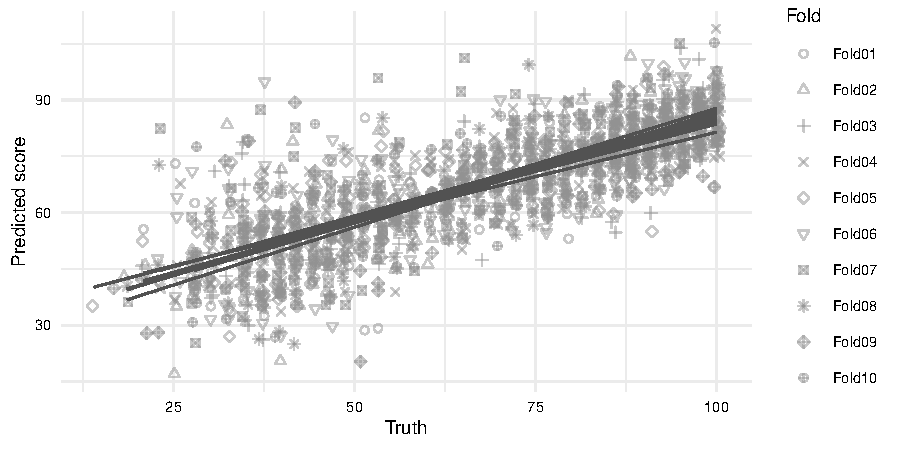
\includegraphics{part_4/9_predict_files/figure-pdf/fig-predict-reg-lr-eval-rmse-1.pdf}

}

\caption{\label{fig-predict-reg-lr-eval-rmse}Distribution of the RMSE
for the cross-validated linear regression model}

\end{figure}%

\end{example}

From Figure~\ref{fig-predict-reg-lr-eval-rmse}, we see data points for
each predicted and truth value pair for each of the ten folds. There is
a trend line for each fold which shows the linear relationship between
the predicted and truth values for each fold. The trend lines are more
similar than different, which is a good sign that the model is not
wildly overfitting the training data. Looking closer, however, we can
see the errors. Some are noticeably distant from the linear trend lines,
\emph{i.e.} outliers, in particular for test scores in the lower ranges.

If the \(R^2\) value is in the ballpark, this means that somewhere
around 40\% of the variation is not explained by the frequency of the
top 1,050 words. This is not surprising, as there are many other factors
that contribute to the proficiency level of a text.

We have a model that is performing better than the null model, but it is
not performing well enough to be very useful. We will need to update the
model specification and/ or the features to try to improve the model
fit. Let's start with the model. There are many different model
specifications we could try, but we will likely need to use a more
complex model specification to capture the complexity that we observe in
the errors from the current linear regression model.

Let's try a decision tree model. \textbf{Decision trees} are models that
are able to model non-linear relationships and interactions between the
features and the outcome and tend to be less influenced by outliers.
Furthermore, decision trees are interpretable, which is a nice feature
for an exploratory-oriented analysis. These are all desirable
characteristics. Decision trees, however, can be prone to overfitting.
For this reason, we will tune the maximum depth of the tree to minimize
overfitting.

To implement a new model in \texttt{tidymodels}, we need to create a new
model specification and a new workflow. We will use the
\texttt{decision\_tree()} function from \{parsnip\} to create the model
specification. The \texttt{decision\_tree()} function takes a
\texttt{tree\_depth} argument that we want to tune. We create the new
model specification with the tuning placeholder in
Example~\ref{exm-predict-reg-model-spec-decision-tree}.

\begin{example}[]\protect\hypertarget{exm-predict-reg-model-spec-decision-tree}{}\label{exm-predict-reg-model-spec-decision-tree}

~

\begin{Shaded}
\begin{Highlighting}[]
\CommentTok{\# Create model specification}
\NormalTok{reg\_spec }\OtherTok{\textless{}{-}}
  \FunctionTok{decision\_tree}\NormalTok{(}\AttributeTok{tree\_depth =} \FunctionTok{tune}\NormalTok{()) }\SpecialCharTok{|\textgreater{}}
  \FunctionTok{set\_engine}\NormalTok{(}\StringTok{"rpart"}\NormalTok{) }\SpecialCharTok{|\textgreater{}}
  \FunctionTok{set\_mode}\NormalTok{(}\StringTok{"regression"}\NormalTok{)}

\CommentTok{\# Preview}
\NormalTok{reg\_spec}
\end{Highlighting}
\end{Shaded}

\begin{Shaded}
\begin{Highlighting}[]
\NormalTok{Decision Tree Model Specification (regression)}

\NormalTok{Main Arguments:}
\NormalTok{  tree\_depth = tune()}

\NormalTok{Computational engine: rpart}
\end{Highlighting}
\end{Shaded}

\end{example}

With the model and tuning specification in place, we can now continue
through the steps outlined in Table~\ref{tbl-workflow} for this decision
tree model. To create the grid of values for the tree depth
hyperparameter, we will include the \texttt{grid\_regular()} function
with 10 levels, as seen in
Snippet~\ref{lst-predict-reg-decision-tree-depth}.

\begin{codelisting}

\caption{\label{lst-predict-reg-decision-tree-depth}Tuning values for
the tree depth hyperparameter}

\centering{

\begin{Shaded}
\begin{Highlighting}[]
\NormalTok{reg\_grid }\OtherTok{\textless{}{-}}
  \FunctionTok{grid\_regular}\NormalTok{(}\FunctionTok{tree\_depth}\NormalTok{(), }\AttributeTok{levels =} \DecValTok{10}\NormalTok{)}
\end{Highlighting}
\end{Shaded}

}

\end{codelisting}%

We can collect the metrics and inspect the RMSE and \(R^2\) values. The
code is seen in Example~\ref{exm-predict-reg-metrics-tree}.

\begin{example}[]\protect\hypertarget{exm-predict-reg-metrics-tree}{}\label{exm-predict-reg-metrics-tree}

~

\begin{Shaded}
\begin{Highlighting}[]
\CommentTok{\# Collect metrics}
\NormalTok{reg\_tree\_cv }\SpecialCharTok{|\textgreater{}} \FunctionTok{collect\_metrics}\NormalTok{()}
\end{Highlighting}
\end{Shaded}

\begin{verbatim}
# A tibble: 2 x 6
  .metric .estimator   mean     n std_err .config             
  <chr>   <chr>       <dbl> <int>   <dbl> <chr>               
1 rmse    standard   15.9      10  0.256  Preprocessor1_Model1
2 rsq     standard    0.510    10  0.0210 Preprocessor1_Model1
\end{verbatim}

\end{example}

The performance for the decision tree is worse than the regularized
linear regression model. The RSME is 15.9 and the \(R^2\) is 0.51. And,
if we compare the standard error between the two models, we can see that
the decision tree model has a lower standard error. This means that the
decision tree model is likely overfitting, despite our efforts to tune
tree depth.

Given the sensitivity of the decision tree branching process and random
initialization, it is possible that the decision tree model is capturing
too much nuance, and not enough generalities. Re-running the model with
a different seed may result in a different model. This is a limitation
with decision tree models, but it is also a feature, if we consider
combining multiple decision trees to make a prediction. This is the
basis of \textbf{ensemble models}. An ensemble model is a model that
combines multiple models with the goal to draw out the strengths of each
model and minimize the weaknesses.

A \textbf{random forest} is an ensemble model that combines multiple
decision trees to make a prediction. In addition, random forests also
perform random feature selection. This helps to reduce the correlation
between the decision trees and thus works to reduce the overall variance
of the model.

Let's try a random forest model to address our text regression task. We
will use the \texttt{rand\_forest()} function from \{parsnip\} to create
the model specification. The \texttt{rand\_forest()} function also takes
a hyperparameter for the number of trees to be used in the model. We
will select the \texttt{ranger} engine. Additionally, we will add the
\texttt{importance} argument to ensure that we can extract feature
importance if this model proves to be useful. We create the new model
specification in Example~\ref{exm-predict-reg-model-spec-random-forest}.

\begin{example}[]\protect\hypertarget{exm-predict-reg-model-spec-random-forest}{}\label{exm-predict-reg-model-spec-random-forest}

~

\begin{Shaded}
\begin{Highlighting}[]
\CommentTok{\# Create model specification}
\NormalTok{reg\_spec }\OtherTok{\textless{}{-}}
  \FunctionTok{rand\_forest}\NormalTok{(}\AttributeTok{trees =} \FunctionTok{tune}\NormalTok{()) }\SpecialCharTok{|\textgreater{}}
  \FunctionTok{set\_engine}\NormalTok{(}\StringTok{"ranger"}\NormalTok{, }\AttributeTok{importance =} \StringTok{"impurity"}\NormalTok{) }\SpecialCharTok{|\textgreater{}}
  \FunctionTok{set\_mode}\NormalTok{(}\StringTok{"regression"}\NormalTok{)}

\CommentTok{\# Preview}
\NormalTok{reg\_spec}
\end{Highlighting}
\end{Shaded}

\begin{Shaded}
\begin{Highlighting}[]
\NormalTok{Random Forest Model Specification (regression)}

\NormalTok{Main Arguments:}
\NormalTok{  trees = tune()}

\NormalTok{Engine{-}Specific Arguments:}
\NormalTok{  importance = impurity}

\NormalTok{Computational engine: ranger}
\end{Highlighting}
\end{Shaded}

\end{example}

\begin{tcolorbox}[enhanced jigsaw, left=2mm, toprule=.15mm, colback=white, colframe=quarto-callout-color-frame, arc=.35mm, rightrule=.15mm, bottomrule=.15mm, leftrule=.75mm, breakable, opacityback=0]

\textbf{\faIcon{lightbulb} Consider this}

The model building process is iterative and many of the steps are the
same. This is a good indication that creating a custom function to build
and tune the model would be a good idea.

Consider the following: What would you include in the function? What
would you leave out? What required and/ or optional arguments would you
include? What would you hard code? What would you return?

\end{tcolorbox}

Again, we apply the steps in Table~\ref{tbl-workflow} to build and tune
the random forest model. As part of this process, I will limit the range
of the number of trees from 100 to 500 in five levels in the tuning
grid, as seen in Snippet~\ref{lst-predict-reg-random-forest-trees}.

\begin{codelisting}

\caption{\label{lst-predict-reg-random-forest-trees}Tuning values for
the number of trees hyperparameter}

\centering{

\begin{Shaded}
\begin{Highlighting}[]
\NormalTok{reg\_grid }\OtherTok{\textless{}{-}}
  \FunctionTok{grid\_regular}\NormalTok{(}\FunctionTok{trees}\NormalTok{(}\AttributeTok{range =} \FunctionTok{c}\NormalTok{(}\DecValTok{100}\NormalTok{, }\DecValTok{500}\NormalTok{)), }\AttributeTok{levels =} \DecValTok{5}\NormalTok{)}
\end{Highlighting}
\end{Shaded}

}

\end{codelisting}%

Let's collect the metrics and inspect the RMSE and \(R^2\) values. The
code is seen in Example~\ref{exm-predict-reg-metrics-rf}.

\begin{example}[]\protect\hypertarget{exm-predict-reg-metrics-rf}{}\label{exm-predict-reg-metrics-rf}

~

\begin{Shaded}
\begin{Highlighting}[]
\CommentTok{\# Collect metrics}
\NormalTok{reg\_rf\_cv }\SpecialCharTok{|\textgreater{}} \FunctionTok{collect\_metrics}\NormalTok{()}
\end{Highlighting}
\end{Shaded}

\begin{verbatim}
# A tibble: 2 x 6
  .metric .estimator   mean     n std_err .config             
  <chr>   <chr>       <dbl> <int>   <dbl> <chr>               
1 rmse    standard   12.9      10  0.320  Preprocessor1_Model1
2 rsq     standard    0.697    10  0.0164 Preprocessor1_Model1
\end{verbatim}

\end{example}

The random forest model performs better than the decision tree model and
the regularized linear regression model. The RSME is 12.9 and the
\(R^2\) is 0.697. We also see that the standard error falls between the
models we have tried so far.

Before we settle on this model, let's try one more model. In this case,
we will introduce a neural network model. Neural networks are models
that are able to model non-linear relationships and interactions between
the features and the outcome. They are also able to model complex
relationships between the features and the outcome. We will use the
\texttt{mlp()} function from \{parsnip\} to create the model
specification. We will choose the \texttt{brulee} engine which allows us
to tune the learning rate. The \textbf{learning rate} is a
hyperparameter that controls the size of the steps that the model takes
to update the weights.

We create the new model specification with the tuning placeholder in
Example~\ref{exm-predict-reg-model-spec-mlp}.

\begin{example}[]\protect\hypertarget{exm-predict-reg-model-spec-mlp}{}\label{exm-predict-reg-model-spec-mlp}

~

\begin{Shaded}
\begin{Highlighting}[]
\CommentTok{\# Create model specification}
\NormalTok{reg\_spec }\OtherTok{\textless{}{-}}
  \FunctionTok{mlp}\NormalTok{(}\AttributeTok{learn\_rate =} \FunctionTok{tune}\NormalTok{()) }\SpecialCharTok{|\textgreater{}}
  \FunctionTok{set\_engine}\NormalTok{(}\StringTok{"brulee"}\NormalTok{) }\SpecialCharTok{|\textgreater{}}
  \FunctionTok{set\_mode}\NormalTok{(}\StringTok{"regression"}\NormalTok{)}

\CommentTok{\# Preview}
\NormalTok{reg\_spec}
\end{Highlighting}
\end{Shaded}

\begin{Shaded}
\begin{Highlighting}[]
\NormalTok{Single Layer Neural Network Model Specification (regression)}

\NormalTok{Main Arguments:}
\NormalTok{  learn\_rate = tune()}

\NormalTok{Computational engine: brulee}

\NormalTok{Model fit template:}
\NormalTok{brulee::brulee\_mlp(x = missing\_arg(), y = missing\_arg(), learn\_rate = tune())}
\end{Highlighting}
\end{Shaded}

\end{example}

And include the code in Snippet~\ref{lst-predict-reg-mlp-learning-rate}
to create a grid of values for the learning rate hyperparameter, as part
of the model building workflow.

\begin{codelisting}

\caption{\label{lst-predict-reg-mlp-learning-rate}Tuning values for the
learning rate hyperparameter}

\centering{

\begin{Shaded}
\begin{Highlighting}[]
\NormalTok{reg\_grid }\OtherTok{\textless{}{-}}
  \FunctionTok{grid\_regular}\NormalTok{(}\FunctionTok{learn\_rate}\NormalTok{(), }\AttributeTok{levels =} \DecValTok{10}\NormalTok{)}
\end{Highlighting}
\end{Shaded}

}

\end{codelisting}%

Let's collect the metrics and inspect the RMSE and \(R^2\) values. The
code is seen in Example~\ref{exm-predict-reg-metrics-mlp}.

\begin{example}[]\protect\hypertarget{exm-predict-reg-metrics-mlp}{}\label{exm-predict-reg-metrics-mlp}

~

\begin{Shaded}
\begin{Highlighting}[]
\CommentTok{\# Collect metrics}
\NormalTok{reg\_mlp\_cv }\SpecialCharTok{|\textgreater{}} \FunctionTok{collect\_metrics}\NormalTok{()}
\end{Highlighting}
\end{Shaded}

\begin{verbatim}
# A tibble: 2 x 6
  .metric .estimator   mean     n std_err .config             
  <chr>   <chr>       <dbl> <int>   <dbl> <chr>               
1 rmse    standard   16.9      10  1.57   Preprocessor1_Model1
2 rsq     standard    0.443    10  0.0978 Preprocessor1_Model1
\end{verbatim}

\end{example}

So in summary, we've tried four different model specifications. The
regularized linear regression model, the decision tree model, the random
forest model, and the neural network model. The random forest model
performed the best. For each of these models, however, we have only
tried word features measured by \(tf\)-\(idf\). We could imagine that
the performance of these models could be improved by varying the
features to include bigrams, for example. We could also explore
different measures of word usage. Furthermore, for some of our models,
we could try different engines and/ or hyperparameters (some have more
than one!).

We could continue to try to explore these possible combinations, and you
likely would in your research. But at this point we have a model that is
performing better than the null model and is performing better than the
other models we have tried. So we will consider this model to be good
enough for our purposes.

Let's take our Random Forest model, fit it to our training data, apply
it to the testing data, and collect the metrics on the test set. The
code is seen in
Example~\ref{exm-predict-reg-model-spec-random-forest-workflow-tune-fit}.

\begin{example}[]\protect\hypertarget{exm-predict-reg-model-spec-random-forest-workflow-tune-fit}{}\label{exm-predict-reg-model-spec-random-forest-workflow-tune-fit}

~

\begin{Shaded}
\begin{Highlighting}[]
\CommentTok{\# Fit the model to the training set and}
\CommentTok{\# evaluate on the test set}
\NormalTok{reg\_final\_fit }\OtherTok{\textless{}{-}}
  \FunctionTok{last\_fit}\NormalTok{(}
\NormalTok{    reg\_wf\_rf,}
    \AttributeTok{split =}\NormalTok{ reg\_split}
\NormalTok{  )}

\CommentTok{\# Evaluate model on testing set}
\NormalTok{reg\_final\_fit }\SpecialCharTok{|\textgreater{}} \FunctionTok{collect\_metrics}\NormalTok{()}
\end{Highlighting}
\end{Shaded}

\begin{verbatim}
# A tibble: 2 x 4
  .metric .estimator .estimate .config             
  <chr>   <chr>          <dbl> <chr>               
1 rmse    standard      12.9   Preprocessor1_Model1
2 rsq     standard       0.689 Preprocessor1_Model1
\end{verbatim}

\end{example}

Ok. The difference between the cross-validated metrics and the metrics
for the test set differ --but only slightly. This suggests that the
model is robust and that we have not overfit the data from the training
set.

Now, our likely goal as an academic is to understanding something about
the features that contribute to the performance of the model. So let's
approach extracting feature importance from the Random Forest model we
build with the \texttt{ranger} engine. Remember, we added an
\texttt{importance} argument to the \texttt{set\_engine()} function and
set it to `impurity'. We can now take advantage by using \{vip\} to
extract the feature importance. The code is seen in
Example~\ref{exm-predict-reg-final-fit-vip}.

\begin{example}[]\protect\hypertarget{exm-predict-reg-final-fit-vip}{}\label{exm-predict-reg-final-fit-vip}

~

\begin{Shaded}
\begin{Highlighting}[]
\CommentTok{\# Extract feature importance}
\NormalTok{reg\_vip }\OtherTok{\textless{}{-}}
\NormalTok{  reg\_final\_fit }\SpecialCharTok{|\textgreater{}}
  \FunctionTok{extract\_fit\_parsnip}\NormalTok{() }\SpecialCharTok{|\textgreater{}}
  \FunctionTok{vi}\NormalTok{(}\AttributeTok{scale =} \ConstantTok{TRUE}\NormalTok{)}

\CommentTok{\# Preview}
\NormalTok{reg\_vip }\SpecialCharTok{|\textgreater{}}
  \FunctionTok{slice\_head}\NormalTok{(}\AttributeTok{n =} \DecValTok{10}\NormalTok{)}
\end{Highlighting}
\end{Shaded}

\begin{verbatim}
# A tibble: 10 x 2
   Variable        Importance
   <chr>                <dbl>
 1 tfidf_text_que       100  
 2 tfidf_text_es         68.8
 3 tfidf_text_una        57.4
 4 tfidf_text_por        57.2
 5 tfidf_text_pero       54.0
 6 tfidf_text_del        48.5
 7 tfidf_text_con        46.1
 8 tfidf_text_se         44.9
 9 tfidf_text_para       44.1
10 tfidf_text_muy        43.6
\end{verbatim}

\end{example}

We can now visualize the feature importance of the model. The code is
seen in Example~\ref{exm-predict-reg-final-fit-vip-visualize}.

\begin{example}[]\protect\hypertarget{exm-predict-reg-final-fit-vip-visualize}{}\label{exm-predict-reg-final-fit-vip-visualize}

~

\begin{Shaded}
\begin{Highlighting}[]
\CommentTok{\# Extract predictions}
\NormalTok{reg\_vip }\SpecialCharTok{|\textgreater{}}
  \FunctionTok{mutate}\NormalTok{(}\AttributeTok{Variable =} \FunctionTok{str\_replace}\NormalTok{(Variable, }\StringTok{"\^{}tfidf\_text\_"}\NormalTok{, }\StringTok{""}\NormalTok{)) }\SpecialCharTok{|\textgreater{}}
  \FunctionTok{slice\_max}\NormalTok{(Importance, }\AttributeTok{n =} \DecValTok{20}\NormalTok{) }\SpecialCharTok{|\textgreater{}}
  \CommentTok{\# reorder variables by importance}
  \FunctionTok{ggplot}\NormalTok{(}\FunctionTok{aes}\NormalTok{(}\FunctionTok{reorder}\NormalTok{(Variable, Importance), Importance)) }\SpecialCharTok{+}
  \FunctionTok{geom\_point}\NormalTok{() }\SpecialCharTok{+}
  \FunctionTok{coord\_flip}\NormalTok{() }\SpecialCharTok{+}
  \FunctionTok{labs}\NormalTok{(}
    \AttributeTok{x =} \StringTok{"Feature"}\NormalTok{,}
    \AttributeTok{y =} \StringTok{"Importance"}
\NormalTok{  )}
\end{Highlighting}
\end{Shaded}

\begin{figure}[!htb]

\centering{

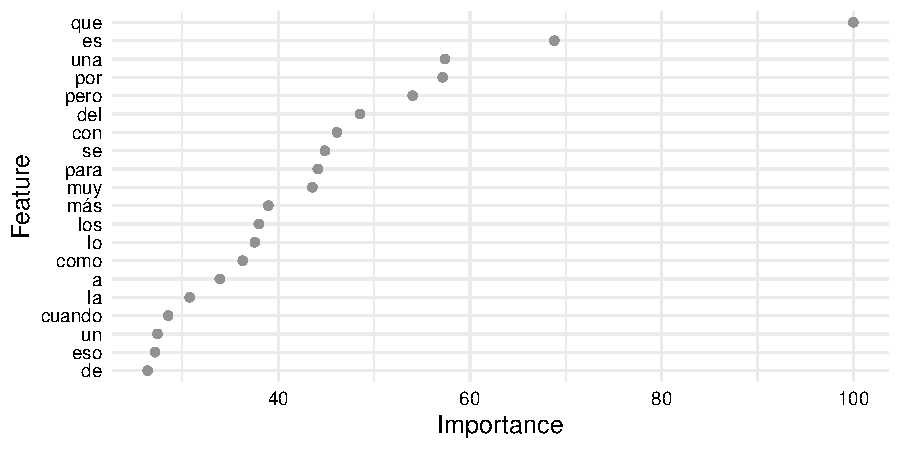
\includegraphics{part_4/9_predict_files/figure-pdf/fig-predict-reg-final-fit-vip-visualize-1.pdf}

}

\caption{\label{fig-predict-reg-final-fit-vip-visualize}Feature
importance of the random forest model}

\end{figure}%

\end{example}

In this section, we've built text regression models focusing on the
ability to change algorithms and hyperparameters. We also seen some of
the differences between evaluating model performance between
classification and regression tasks. There are many more combinations of
model specifications and feature selection and engineering that can be
applied. In your research, you will find yourself using these tools to
explore the best model for your data.

\section*{Activities}\label{activities-7}
\addcontentsline{toc}{section}{Activities}

\markright{Activities}

In the following activities, we will apply the concepts and techniques
we have learned in this chapter. We will use the Tidymodels framework to
build and evaluate supervised machine learning models for text
classification and regression tasks.

\begin{tcolorbox}[enhanced jigsaw, left=2mm, toprule=.15mm, colback=white, colframe=quarto-callout-color-frame, arc=.35mm, rightrule=.15mm, bottomrule=.15mm, leftrule=.75mm, breakable, opacityback=0]

\textbf{\faIcon{file-code} Recipe}

\textbf{What}: Building predictive models\\
\textbf{How}: Read Recipe 9, complete comprehension check, and prepare
for Lab 9.\\
\textbf{Why}: To continue to build experience building predictive models
with the Tidymodels framework.

\end{tcolorbox}

\begin{tcolorbox}[enhanced jigsaw, left=2mm, toprule=.15mm, colback=white, colframe=quarto-callout-color-frame, arc=.35mm, rightrule=.15mm, bottomrule=.15mm, leftrule=.75mm, breakable, opacityback=0]

\textbf{\faIcon{flask} Lab}

\textbf{What}: Text classification\\
\textbf{How}: Clone, fork, and complete the steps in Lab 9.\\
\textbf{Why}: To apply your knowledge of supervised machine learning to
a text classification task.

\end{tcolorbox}

\section*{Summary}\label{summary-8}
\addcontentsline{toc}{section}{Summary}

\markright{Summary}

In this chapter, we outlined the workflow for approach predictive
modeling and the Tidymodels framework. We then applied the workflow to
text classification and regression tasks. Gained experience identifying,
selecting, and engineering features on the one hand, and building and
tuning models on the other. To evaluate the models, we used
cross-validation for performance and finalized our interpretation with
techniques to extract feature importance.

\chapter{Infer}\label{sec-infer-chapter}

\begin{quote}
People generally see what they look for, and hear what they listen for.

--- Harper Lee, To Kill a Mockingbird
\end{quote}

\begin{tcolorbox}[enhanced jigsaw, left=2mm, toprule=.15mm, colback=white, colframe=quarto-callout-color-frame, arc=.35mm, rightrule=.15mm, bottomrule=.15mm, leftrule=.75mm, breakable, opacityback=0]

\textbf{\faIcon{list-alt} Outcomes}

\begin{itemize}
\tightlist
\item
  Identify the research goals of inferential data analysis
\item
  Describe the workflow for inferential data analysis
\item
  Indicate the importance of quantifying uncertainty in inferential data
  analysis
\end{itemize}

\end{tcolorbox}

In this chapter, we consider approaches to deriving knowledge from
information which can be generalized to the population from which the
data is sampled. This process is known as statistical inference. The
discussion here implements descriptive assessments, statistical tests,
and evaluation procedures for a series of contexts which are common in
the analysis of corpus-based data. During our treatment of these
contexts, we will establish a foundational understanding of statistical
inference using a simulation-based approach.

\begin{tcolorbox}[enhanced jigsaw, left=2mm, toprule=.15mm, colback=white, colframe=quarto-callout-color-frame, arc=.35mm, rightrule=.15mm, bottomrule=.15mm, leftrule=.75mm, breakable, opacityback=0]

\textbf{\faIcon{terminal} Lessons}

\textbf{What}: Advanced Tables\\
\textbf{How}: In an R console, load \{swirl\}, run \texttt{swirl()}, and
follow prompts to select the lesson.\\
\textbf{Why}: To explore how to enhance dataset summaries using
\{janitor\} and present them effectively with \{kableExtra\}'s advanced
formatting options.

\end{tcolorbox}

\section{Orientation}\label{sec-infer-orientation}

In contrast to exploratory and predictive analyses, inference is not a
data-driven endeavor. Rather, the goal of inferential data analysis
(IDA) is to make theoretical claims about the population and assess the
extent to which the data supports those claims. This implicates two key
methodological restrictions which are not in play in other analysis
methods.

First, the research question and expected findings are formulated
\emph{before} the data is analyzed, in fact strictly speaking this
should take place even before data collection. This helps ensure that
the data is aligned with the research question and that the data is
representative of the population and that the analysis has a targeted
focus and does not run the risk of becoming a `just-so' story\footnote{``Hypothesis
  After Result is Known'' (HARKing) involves selectively analyzing data,
  trying different variables or combinations until a significant
  \(p\)-value is obtained, or stopping data collection when a
  significant result is found (\citeproc{ref-Kerr1998}{Kerr, 1998}).} or
a `significance-finding' mission\footnote{``p-hacking'' is the practice
  of running multiple tests until a statistically significant result is
  found. This practice violates the principles of significance testing
  (\citeproc{ref-Head2015}{Head, Holman, Lanfear, Kahn, \& Jennions,
  2015}).} both of which violate the principles of significance testing.

Second, the data used in IDA is only used once. That is to say, that the
entire dataset is used a single time to statistically interrogate the
relationship(s) of interest. In both EDA and PDA the data can be
approached multiple times in different ways and the results of the
analysis can be used to inform the next steps in the analysis. In IDA,
however, the data is used to test a specific hypothesis and the results
of the analysis are interpreted in the context of that hypothesis.

The methodological approach to inferential data analysis (IDA) is the
most straightforward of the analysis types covered in this textbook. As
the research goal is to test a claim, the steps necessary are fewer than
in EDA or PDA, where the exploratory nature of these approaches includes
various possible iterations. The workflow for IDA is shown in
Table~\ref{tbl-infer-workflow}.

\begin{longtable}[]{@{}
  >{\raggedright\arraybackslash}p{(\columnwidth - 4\tabcolsep) * \real{0.0500}}
  >{\raggedright\arraybackslash}p{(\columnwidth - 4\tabcolsep) * \real{0.1500}}
  >{\raggedright\arraybackslash}p{(\columnwidth - 4\tabcolsep) * \real{0.8000}}@{}}
\caption{Workflow for inferential data
analysis}\label{tbl-infer-workflow}\tabularnewline
\toprule\noalign{}
\begin{minipage}[b]{\linewidth}\raggedright
Step
\end{minipage} & \begin{minipage}[b]{\linewidth}\raggedright
Name
\end{minipage} & \begin{minipage}[b]{\linewidth}\raggedright
Description
\end{minipage} \\
\midrule\noalign{}
\endfirsthead
\toprule\noalign{}
\begin{minipage}[b]{\linewidth}\raggedright
Step
\end{minipage} & \begin{minipage}[b]{\linewidth}\raggedright
Name
\end{minipage} & \begin{minipage}[b]{\linewidth}\raggedright
Description
\end{minipage} \\
\midrule\noalign{}
\endhead
\bottomrule\noalign{}
\endlastfoot
1 & Identify & Identify and map the hypothesis statement to the
appropriate response and explanatory variables \\
2 & Inspect & Assess the distribution of the variable(s) with the
appropriate descriptive statistics and visualizations. \\
3 & Interrogate & Apply the appropriate statistical procedure to the
dataset. \\
4 & Interpret & Review the statistical results and interpret them in the
context of the hypothesis. \\
\end{longtable}

Based on the hypothesis statement, we first identify and operationalize
the variables. The response variable whose variation we aim to explain.
In most statistical designs, one or more explanatory variables are
included in the analysis in an attempt to gauge the extent to which
these variables account for the variation in the response variable. For
both response and explanatory variables, it is key to confirm that your
operationalization of the variables is well-defined and that the data
aligns.

\begin{tcolorbox}[enhanced jigsaw, left=2mm, toprule=.15mm, colback=white, colframe=quarto-callout-color-frame, arc=.35mm, rightrule=.15mm, bottomrule=.15mm, leftrule=.75mm, breakable, opacityback=0]

\textbf{\faIcon{lightbulb} Consider this}

What are the explanatory and/ or response variables in each of these
statements? How are these variables operationalized? What key sampling
features are necessary for the data to test these hypotheses?

\begin{enumerate}
\def\labelenumi{\arabic{enumi}.}
\tightlist
\item
  There will be statistically significant differences in the kinds of
  collocations used in English dialects spoken in urban areas compared
  to those spoken in rural areas.
\item
  French L2 learners will make more vocabulary errors in oral production
  than in written production.
\item
  The association strength between Mandarin words and their English
  translations will be a significant predictor of translation difficulty
  for novice translators.
\item
  The prevalence of gender-specific words in German-speaking communities
  on distinct online forums will significantly reflect gender roles.
\item
  The frequency of function words used by Spanish L2 learners will be a
  significant predictor of their stage in language acquisition.
\end{enumerate}

\end{tcolorbox}

Next, we determine the informational values of the variables. The
informational value of each variable will condition how we approach
visualization, interrogation, and ultimately interpretation of the
results. Note, that some informational types can be converted to other
types, specifically higher-order types can be converted to lower-order
types. For example, a continuous variable can be converted to a
categorical variable, but not vice versa. It is preferable, however, to
use the highest informational value of a variable. Simplifying data
results in a loss of information --which will result in a loss of
information and hence statistical power which may lead to results that
obscure meaningful patterns in the data (\citeproc{ref-Baayen2004}{R.
Harald Baayen, 2004}).

With our design in place, we can now inspect the data. This involves
assessing the distribution of the variables using descriptive statistics
and visualizations. The goal of this step is to confirm the integrity of
the data (missing data, anomalies, \emph{etc}.), identify general
patterns in the data, and identify potential outliers. As much as this
is a verification step, it also serves to provide a sense of the data
and the extent to which the data aligns with the hypothesis. This is
particularly true when statistical designs are complex and involve
multiple explanatory variables. An appropriate visualization provides
context for interpreting the results of the statistical analysis.

Interrogating the data involves applying the appropriate statistical
procedure to the dataset. In the \textbf{Null Hypothesis Significance
Testing} (NHST) paradigm, this process includes calculating a statistic
from the data, comparing it to a null hypothesis distribution, and
measuring the evidence against the null hypothesis. The null hypothesis
distribution is a distribution of statistic values that we would expect
if the null hypothesis were true, \emph{i.e.} that there is no
difference or relationship between the explanatory and/ or response
variables. By comparing the observed statistic to the null hypothesis
distribution, we can determine the likelihood of observing the observed
statistic, if the null hypothesis were true. The estimate of this
likelihood is a \textbf{\(p\)-value}. When the \(p\)-value is below a
pre-determined threshold, typically 0.05, the result is considered
statistically significant. This means that the observed statistic is
sufficiently different from the null hypothesis distribution that we can
reject the null hypothesis.

Now let's consider how to approach interpreting the results from a
statistical test. The \(p\)-value provides a probability that the
results of our statistical test could be explained by the null
hypothesis. When this probability is below the threshold of 0.05, the
result is considered statistically significant, otherwise we have a
`null result' (\emph{i.e.} non-significant).

However, this sets up a binary distinction that can be problematic. On
the one hand, what is one to do if a test returns a \(p\)-value of
0.051? According to standard practice these ``marginally significant''
results would not be statistically significant. On the other hand, if we
get a statistically significant result, say a \(p\)-value of 0.49, do we
move on --case closed? To address both of these issues, it is important
to calculate a confidence interval for the test statistic. The
\textbf{confidence interval} is the range of values for our test
statistic that we would expect the true statistic value to fall within
some level of uncertainty. Again, 95\% is the most common level of
uncertainty. The upper and lower bounds of this range are called the
confidence limits for the test statistic.

Used in conjunction with \(p\)-values, confidence intervals can provide
a more nuanced interpretation of the results of a statistical test. For
example, if we get a \(p\)-value of .051, but the confidence interval is
very narrow, we can be more confident that the results are reliable.
Conversely, if we get a \(p\)-value of .049, but the confidence interval
is very wide, we can be less confident that the results are reliable. If
our confidence interval contains the null value, then even a significant
\(p\)-value will require a more nuanced interpretation.

\begin{tcolorbox}[enhanced jigsaw, left=2mm, toprule=.15mm, colback=white, colframe=quarto-callout-color-frame, arc=.35mm, rightrule=.15mm, bottomrule=.15mm, leftrule=.75mm, breakable, opacityback=0]

\textbf{\faIcon{medal} Dive deeper}

Overgeneralization and undergeneralization are more formally known as
Type I and Type II error, respectively. \textbf{Type I error} (false
positive) occurs when we reject the null hypothesis when it is true.
That is, we erroneously detect a significant result, when in fact the
tested relationship is not borne out in the population. \textbf{Type II
error} (false negative) occurs when we fail to reject the null
hypothesis when it is false. This is a case of missing a significant
result due to the limitations of the analysis which can stem from the
sample size, the design of the study, or the statistical test used.

\end{tcolorbox}

It is important to underscore that the purpose of IDA is to draw
conclusions from a dataset which are generalizable to the population.
These conclusions require that there are rigorous measures to ensure
that the results of the analysis do not overgeneralize (suggest there is
a relationship when there is not one) and balance that with the fact
that we don't want to undergeneralize (miss the fact that there is an
relationship in the population, but our analysis was not capable of
detecting it).

\section{Analysis}\label{sec-infer-analysis}

In this section, we will discuss the practical application of
inferential data analysis. The discussion will be divided into two
sections based on the type of response variable: categorical and
numeric. We will then explore specific designs for univariate,
bivariate, and multivariate tests. We will learn and implement null
significance testing using a simulation-based workflow. In contrast to
theory-based methods, simulation-based methods tend to be more
intuitive, easier to implement, and provide a better conceptual
understanding of the statistical designs and analyses
(\citeproc{ref-Morris2019}{Morris, White, \& Crowther, 2019};
\citeproc{ref-Rossman2014a}{Rossman \& Chance, 2014}).

The steps for implementing a simulation-based approach to significance
testing are outlined in Table~\ref{tbl-infer-simulation}.

\begin{longtable}[]{@{}
  >{\raggedright\arraybackslash}p{(\columnwidth - 4\tabcolsep) * \real{0.0500}}
  >{\raggedright\arraybackslash}p{(\columnwidth - 4\tabcolsep) * \real{0.2500}}
  >{\raggedright\arraybackslash}p{(\columnwidth - 4\tabcolsep) * \real{0.7000}}@{}}
\caption{Simulation-based workflow for significance
testing}\label{tbl-infer-simulation}\tabularnewline
\toprule\noalign{}
\begin{minipage}[b]{\linewidth}\raggedright
Step
\end{minipage} & \begin{minipage}[b]{\linewidth}\raggedright
Name
\end{minipage} & \begin{minipage}[b]{\linewidth}\raggedright
Description
\end{minipage} \\
\midrule\noalign{}
\endfirsthead
\toprule\noalign{}
\begin{minipage}[b]{\linewidth}\raggedright
Step
\end{minipage} & \begin{minipage}[b]{\linewidth}\raggedright
Name
\end{minipage} & \begin{minipage}[b]{\linewidth}\raggedright
Description
\end{minipage} \\
\midrule\noalign{}
\endhead
\bottomrule\noalign{}
\endlastfoot
1 & Specify & Specify the variables of interest and their
relationship \\
2 & Calculate & Calculate the observed statistic \\
3 & Hypothesize & Generate the null hypothesis distribution \\
4 & Get \(p\)-value & Calculate the \(p\)-value \\
5 & Get confidence interval & Calculate the confidence interval \\
\end{longtable}

\{infer\} (\citeproc{ref-R-infer}{Bray et al., 2024}) provides a
Tidyverse-friendly framework to implement simulation-based methods for
statistical inference. Designed to be used in conjunction with
\{tidyverse\}, \{infer\} provides a set of functions that can be used to
specify the variables of interest, calculate the observed statistic,
generate the null hypothesis distribution and calculate the \(p\)-value
and the confidence interval.

Let's load the necessary packages we will use in this section, as seen
in Example~\ref{exm-infer-setup}.

\begin{example}[]\protect\hypertarget{exm-infer-setup}{}\label{exm-infer-setup}

~

\begin{Shaded}
\begin{Highlighting}[]
\CommentTok{\# Load packages}
\FunctionTok{library}\NormalTok{(infer)      }\CommentTok{\# for statistical inference}
\FunctionTok{library}\NormalTok{(skimr)      }\CommentTok{\# for descriptive statistics}
\FunctionTok{library}\NormalTok{(janitor)    }\CommentTok{\# for cross{-}tabulation}
\end{Highlighting}
\end{Shaded}

\end{example}

\subsection{Categorical}\label{sec-infer-categorical}

Here we demonstrate the application of IDA to categorical response
variables. This will include various common statistical designs and
analyses. In Table~\ref{tbl-infer-cat-design}, we see common design
scenarios, the variables involved, and the statistic used in the
analysis.

\begin{longtable}[]{@{}
  >{\raggedright\arraybackslash}p{(\columnwidth - 6\tabcolsep) * \real{0.2000}}
  >{\raggedright\arraybackslash}p{(\columnwidth - 6\tabcolsep) * \real{0.3500}}
  >{\raggedright\arraybackslash}p{(\columnwidth - 6\tabcolsep) * \real{0.3500}}
  >{\raggedright\arraybackslash}p{(\columnwidth - 6\tabcolsep) * \real{0.1000}}@{}}
\caption{Statistical test designs for categorical response
variables}\label{tbl-infer-cat-design}\tabularnewline
\toprule\noalign{}
\begin{minipage}[b]{\linewidth}\raggedright
Scenario
\end{minipage} & \begin{minipage}[b]{\linewidth}\raggedright
Explanatory variable(s)
\end{minipage} & \begin{minipage}[b]{\linewidth}\raggedright
Statistical test
\end{minipage} & \begin{minipage}[b]{\linewidth}\raggedright
\texttt{infer}
\end{minipage} \\
\midrule\noalign{}
\endfirsthead
\toprule\noalign{}
\begin{minipage}[b]{\linewidth}\raggedright
Scenario
\end{minipage} & \begin{minipage}[b]{\linewidth}\raggedright
Explanatory variable(s)
\end{minipage} & \begin{minipage}[b]{\linewidth}\raggedright
Statistical test
\end{minipage} & \begin{minipage}[b]{\linewidth}\raggedright
\texttt{infer}
\end{minipage} \\
\midrule\noalign{}
\endhead
\bottomrule\noalign{}
\endlastfoot
Univariate & - & Proportion & \texttt{prop} \\
Bivariate & Categorical & Difference in proportions &
\texttt{diff\ in\ props} \\
Bivariate (\textgreater2 levels) & Categorical (3+ levels) & Chi-square
& \texttt{chisq} \\
Multivariate & Categorical or Numeric(2+ variables) & Logistic
regression & \texttt{fit()} \\
\end{longtable}

We will use a derived version of the \texttt{dative} dataset from
\{languageR\}. It contains over 3k observations describing the
realization of the recipient clause in English dative constructions. To
familiarize ourselves with the dataset, let's consider the data
dictionary in Table~\ref{tbl-infer-cat-data-dict}.

\begin{longtable}[]{@{}
  >{\raggedright\arraybackslash}p{(\columnwidth - 6\tabcolsep) * \real{0.1500}}
  >{\raggedright\arraybackslash}p{(\columnwidth - 6\tabcolsep) * \real{0.1500}}
  >{\raggedright\arraybackslash}p{(\columnwidth - 6\tabcolsep) * \real{0.1500}}
  >{\raggedright\arraybackslash}p{(\columnwidth - 6\tabcolsep) * \real{0.5500}}@{}}

\caption{\label{tbl-infer-cat-data-dict}Data dictionary for the
\texttt{dative\_tbl} dataset.}

\tabularnewline

\toprule\noalign{}
\begin{minipage}[b]{\linewidth}\raggedright
variable
\end{minipage} & \begin{minipage}[b]{\linewidth}\raggedright
name
\end{minipage} & \begin{minipage}[b]{\linewidth}\raggedright
type
\end{minipage} & \begin{minipage}[b]{\linewidth}\raggedright
description
\end{minipage} \\
\midrule\noalign{}
\endhead
\bottomrule\noalign{}
\endlastfoot
rcp\_real & Realization of RCP & categorical & The realization of the
recipient (NP/ PP) \\
modality & Modality & categorical & The modality of the utterance
(spoken/ written) \\
rcp\_len & Length of RCP & numeric & The length of the recipient (number
of words) \\
thm\_len & Length of THM & numeric & The length of the theme (number of
words) \\

\end{longtable}

We see that this dataset has four variables, two categorical and two
numeric. In our demonstrations we are going to use the
\texttt{rcp\_real} as the response variable, the variable whose
variation we are investigating.

For a bit more context, a dative is the phrase which reflects the entity
that takes the recipient role in a ditransitive clause. In English, the
recipient (dative) can be realized as either a prepositional phrase (PP)
as seen in Example~\ref{exm-infer-cat-dative-examples} (1) or as a noun
phrase (NP) as seen in (2).

\begin{example}[]\protect\hypertarget{exm-infer-cat-dative-examples}{}\label{exm-infer-cat-dative-examples}

Dative examples

\begin{enumerate}
\def\labelenumi{(\arabic{enumi})}
\tightlist
\item
  John gave the book {[}to Mary \textsubscript{PP}{]}.
\item
  John gave {[}Mary \textsubscript{NP}{]} the book.
\end{enumerate}

\end{example}

Together these two syntactic options are known as the Dative Alternation
(\citeproc{ref-Bresnan2007}{Bresnan, Cueni, Nikitina, \& Baayen, 2007}).

Let's go ahead and load the dataset, as seen in
Example~\ref{exm-infer-cat-read-dative}.

\begin{example}[]\protect\hypertarget{exm-infer-cat-read-dative}{}\label{exm-infer-cat-read-dative}

~

\begin{Shaded}
\begin{Highlighting}[]
\CommentTok{\# Load datasets}
\NormalTok{dative\_tbl }\OtherTok{\textless{}{-}}
  \FunctionTok{read\_csv}\NormalTok{(}\StringTok{"../data/dative\_ida.csv"}\NormalTok{)}
\end{Highlighting}
\end{Shaded}

\end{example}

In preparation for statistical analysis, I performed a statistical
overview and diagnostics of the dataset. This included checking for
missing data, outliers, and anomalies. I also checked the distribution
of the variables using descriptive statistics and visualizations, noting
that the \texttt{rcp\_len} and \texttt{thm\_len} variables are
right-skewed. This is something to keep in mind. The results of this
overview and diagnostics are not shown here, but they are important
steps in the IDA workflow. In this process, I converted the character
variables to factors as most statistical tests require factors. A
preview of the dataset is shown in
Example~\ref{exm-infer-cat-dative-preview}.

\begin{example}[]\protect\hypertarget{exm-infer-cat-dative-preview}{}\label{exm-infer-cat-dative-preview}

~

\begin{Shaded}
\begin{Highlighting}[]
\CommentTok{\# Preview of the dataset}
\NormalTok{dative\_tbl}
\end{Highlighting}
\end{Shaded}

\begin{verbatim}
# A tibble: 3,263 x 4
   rcp_real modality rcp_len thm_len
   <fct>    <fct>      <dbl>   <dbl>
 1 NP       written        1      14
 2 NP       written        2       3
 3 NP       written        1      13
 4 NP       written        1       5
 5 NP       written        2       3
 6 NP       written        2       4
 7 NP       written        2       4
 8 NP       written        1       1
 9 NP       written        1      11
10 NP       written        1       2
# i 3,253 more rows
\end{verbatim}

\end{example}

We can see that the dataset includes 3,263 observations. We will take a
closer look a the descriptive statistics for the variables as we prepare
for each analysis.

\subsubsection{Univariate analysis}\label{sec-infer-cat-univariate}

The univariate analysis is the simplest statistical design and analysis.
It includes only one variable. The goal is to describe the distribution
of the levels of the variable. The \texttt{rcp\_real} variable has two
levels: NP and PP. A potential research question for a case like this
may aim to test the claim that:

\begin{itemize}
\tightlist
\item
  NP realizations of the recipient clause are the canonical form in
  English dative constructions, and therefore will be the most frequent
  realization of the recipient clause.
\end{itemize}

This hypothesis can be tested using a \textbf{difference in proportion
test}. The null hypothesis is that there is no difference in the
proportion of NP and PP realizations of the recipient clause. The
alternative hypothesis is that NP realizations of the recipient clause
are more frequent than PP realizations of the recipient clause.

Before we get into statistical analysis, it is always a good idea to
cross-tabulate or visualize the question, depending on the complexity of
the relationship. In Example~\ref{exm-infer-cat-univariate-tbl}, we see
the code the shows the distribution of the levels of the
\texttt{rcp\_real} variable in a cross-table.

\begin{example}[]\protect\hypertarget{exm-infer-cat-univariate-tbl}{}\label{exm-infer-cat-univariate-tbl}

~

\begin{Shaded}
\begin{Highlighting}[]
\CommentTok{\# Cross{-}tabulation of \textasciigrave{}rcp\_real\textasciigrave{}}
\NormalTok{dative\_tbl }\SpecialCharTok{|\textgreater{}}
  \FunctionTok{tabyl}\NormalTok{(rcp\_real) }\SpecialCharTok{|\textgreater{}}
  \FunctionTok{adorn\_pct\_formatting}\NormalTok{(}\AttributeTok{digits =} \DecValTok{2}\NormalTok{) }\SpecialCharTok{|\textgreater{}}
  \FunctionTok{kable}\NormalTok{() }\SpecialCharTok{|\textgreater{}}
  \FunctionTok{kable\_styling}\NormalTok{()}
\end{Highlighting}
\end{Shaded}

\begin{longtable}[]{@{}
  >{\raggedright\arraybackslash}p{(\columnwidth - 4\tabcolsep) * \real{0.5000}}
  >{\raggedright\arraybackslash}p{(\columnwidth - 4\tabcolsep) * \real{0.2500}}
  >{\raggedright\arraybackslash}p{(\columnwidth - 4\tabcolsep) * \real{0.2500}}@{}}

\caption{\label{tbl-infer-cat-univariate}Distribution of the levels of
the \texttt{rcp\_real} variable.}

\tabularnewline

\toprule\noalign{}
\begin{minipage}[b]{\linewidth}\raggedright
rcp\_real
\end{minipage} & \begin{minipage}[b]{\linewidth}\raggedright
n
\end{minipage} & \begin{minipage}[b]{\linewidth}\raggedright
percent
\end{minipage} \\
\midrule\noalign{}
\endhead
\bottomrule\noalign{}
\endlastfoot
NP & 2414 & 73.98\% \\
PP & 849 & 26.02\% \\

\end{longtable}

\end{example}

From Table~\ref{tbl-infer-cat-univariate}, we see that the proportion of
NP realizations of the recipient clause is higher than the proportion of
PP realizations of the recipient clause. However, we cannot conclude
that there is a difference in the proportion of NP and PP realizations
of the recipient clause. We need to conduct a statistical test to
determine if the difference is statistically significant.

To determine if the distribution of the levels of the \texttt{rcp\_real}
variable is different from what we would expect if the null hypothesis
were true, we need to calculate the difference observed in the sample
and compare it to the differences observed in many samples where the
null hypothesis is true.

First, let's calculate the proportion of NP and PP realizations of the
recipient clause in the sample. We turn to the \texttt{specify()}
function from \{infer\} to specify the variable of interest, step 1 in
the simulation-based workflow in Table~\ref{tbl-infer-simulation}. In
this case, we only have the response variable. Furthermore, the argument
\texttt{success} specifies the level of the response variable that we
will use as the `success'. The term `success' is used because the
\texttt{specify()} function was designed for binomial variables where
the levels are `success' and `failure', as seen in
Example~\ref{exm-infer-cat-specify}.

\begin{example}[]\protect\hypertarget{exm-infer-cat-specify}{}\label{exm-infer-cat-specify}

~

\begin{Shaded}
\begin{Highlighting}[]
\CommentTok{\# Specify the variable of interest}
\NormalTok{dative\_spec }\OtherTok{\textless{}{-}}
\NormalTok{  dative\_tbl }\SpecialCharTok{|\textgreater{}}
  \FunctionTok{specify}\NormalTok{(}
    \AttributeTok{response =}\NormalTok{ rcp\_real,}
    \AttributeTok{success =} \StringTok{"NP"}
\NormalTok{  )}

\CommentTok{\# Preview}
\NormalTok{dative\_spec}
\end{Highlighting}
\end{Shaded}

\begin{verbatim}
Response: rcp_real (factor)
# A tibble: 3,263 x 1
   rcp_real
   <fct>   
 1 NP      
 2 NP      
 3 NP      
 4 NP      
 5 NP      
 6 NP      
 7 NP      
 8 NP      
 9 NP      
10 NP      
# i 3,253 more rows
\end{verbatim}

\end{example}

The \texttt{dative\_spec} is a data frame with attributes which are used
by \{infer\} to maintain information about the statistical design for
the analysis. In this case, we only have information about what the
response variable is.

Step 2 is to calculate the observed statistic. The \texttt{calculate()}
function is used to calculate the proportion statistic setting
\texttt{stat\ =\ "prop"}, as seen in
Example~\ref{exm-infer-cat-calculate}.

\begin{example}[]\protect\hypertarget{exm-infer-cat-calculate}{}\label{exm-infer-cat-calculate}

~

\begin{Shaded}
\begin{Highlighting}[]
\CommentTok{\# Calculate the proportion statistic}
\NormalTok{dative\_obs }\OtherTok{\textless{}{-}}
\NormalTok{  dative\_spec }\SpecialCharTok{|\textgreater{}}
  \FunctionTok{calculate}\NormalTok{(}\AttributeTok{stat =} \StringTok{"prop"}\NormalTok{)}

\CommentTok{\# Preview}
\NormalTok{dative\_obs}
\end{Highlighting}
\end{Shaded}

\begin{verbatim}
Response: rcp_real (factor)
# A tibble: 1 x 1
   stat
  <dbl>
1 0.740
\end{verbatim}

\end{example}

Note, that the observed statistic, proportion, is the same as the
proportion we calculated in Table~\ref{tbl-infer-cat-univariate}. In
such a simple example, the summary statistic and the observed statistic
are the same. But this simple example shows how choosing the `success'
level of the response variable is important. If we had chosen the `PP'
level as the `success' level, then the observed statistic would be the
proportion of PP realizations of the recipient clause. There is nothing
wrong with choosing the `PP' level as the `success' level, but it would
change the direction of the observed statistic.

Now that we have the observed statistic, our goal will be to determine
if the observed statistic is different from what we would expect if the
null hypothesis were true. To do this, we simulate samples where the
null hypothesis is true, step 3 in our workflow.

Simulation means that we will randomly sample from the
\texttt{dative\_tbl} data frame many times. We need to determine how the
sampling takes place. Since \texttt{rcp\_real} is a variable with only
two levels, the null hypothesis is that both levels are equally likely.
In other words, in a null hypothesis world, NP and PP we would expect
the proportions to roughly be 50/50.

To formalize this hypothesis with \texttt{infer} we use the
\texttt{hypothesize()} function and set the null hypothesis to ``point''
and the proportion to 0.5. Then we can \texttt{generate()} a number of
samples, say 1,000, drawn from our 50/50 world. Finally, the
\texttt{prop} (proportion) statistic is calculated for each of the 1,000
samples and returned in a data frame, as seen in
Example~\ref{exm-infer-cat-null-hypothesis}.

\begin{example}[]\protect\hypertarget{exm-infer-cat-null-hypothesis}{}\label{exm-infer-cat-null-hypothesis}

~

\begin{Shaded}
\begin{Highlighting}[]
\CommentTok{\# Generate the null hypothesis distribution}
\NormalTok{dative\_null }\OtherTok{\textless{}{-}}
\NormalTok{  dative\_spec }\SpecialCharTok{|\textgreater{}}
  \FunctionTok{hypothesize}\NormalTok{(}\AttributeTok{null =} \StringTok{"point"}\NormalTok{, }\AttributeTok{p =} \FloatTok{0.5}\NormalTok{) }\SpecialCharTok{|\textgreater{}}
  \FunctionTok{generate}\NormalTok{(}\AttributeTok{reps =} \DecValTok{1000}\NormalTok{, }\AttributeTok{type =} \StringTok{"draw"}\NormalTok{) }\SpecialCharTok{|\textgreater{}}
  \FunctionTok{calculate}\NormalTok{(}\AttributeTok{stat =} \StringTok{"prop"}\NormalTok{)}

\CommentTok{\# Preview}
\NormalTok{dative\_null}
\end{Highlighting}
\end{Shaded}

\begin{verbatim}
Response: rcp_real (factor)
Null Hypothesis: point
# A tibble: 1,000 x 2
   replicate  stat
       <int> <dbl>
 1         1 0.495
 2         2 0.479
 3         3 0.492
 4         4 0.498
 5         5 0.500
 6         6 0.497
 7         7 0.495
 8         8 0.484
 9         9 0.505
10        10 0.505
# i 990 more rows
\end{verbatim}

\end{example}

The result of Example~\ref{exm-infer-cat-null-hypothesis} is a data
frame with as many rows as there are samples. Each row contains the
proportion statistic for each sample drawn from the hypothesized
distribution that the proportion of NP realizations of the recipient
clause is 0.5.

To appreciate the null hypothesis distribution, we can visualize it
using a histogram. \{infer\} provides a convenient \texttt{visualize()}
function for visualizing distributions, as seen in
Example~\ref{exm-infer-cat-null-hypothesis-vis}.

\begin{example}[]\protect\hypertarget{exm-infer-cat-null-hypothesis-vis}{}\label{exm-infer-cat-null-hypothesis-vis}

~

\begin{Shaded}
\begin{Highlighting}[]
\CommentTok{\# Visualize the null hypothesis distribution}
\NormalTok{dative\_null }\SpecialCharTok{|\textgreater{}} \FunctionTok{visualize}\NormalTok{()}
\end{Highlighting}
\end{Shaded}

\begin{figure}[!htb]

\centering{

\includegraphics{part_4/10_infer_files/figure-pdf/fig-infer-cat-null-hypothesis-1.pdf}

}

\caption{\label{fig-infer-cat-null-hypothesis}Simulation-based null
distribution}

\end{figure}%

\end{example}

In Figure~\ref{fig-infer-cat-null-hypothesis}, we see that on the x-axis
is the proportion statistic of NP realizations of the recipient clause
that we would expect if the null hypothesis were true. For the 1,000
samples, the proportion statistic ranges from 0.47 to 0.52. Importantly
we can appreciate that the most of the proportion statistics are around
0.5, in fact, the mean is 0.5 with a standard deviation of 0.01, which
is what we would expect if the null hypothesis were true. But there is
variation, as we would also expect.

Why would we expect variation? Consider the following analogy. If we
were to flip a fair coin 10 times, we would expect to get 5 heads and 5
tails. But this doesn't always happen. Sometimes we get 6 heads and 4
tails. Sometimes we get 7 heads and 3 tails, and so on. As the number of
flips increases, however, we would expect the proportion of heads to be
closer to 0.5, but there would still be variation. The same is true for
the null hypothesis distribution. As the number of samples increases, we
would expect the proportion of NP realizations of the recipient clause
to be closer to 0.5, but there would still be variation. The question is
whether the observed statistic we obtained from our data, in
Example~\ref{exm-infer-cat-calculate}, is within some level of variation
that we would expect if the null hypothesis were true.

Let's visualize the observed statistic on the null hypothesis
distribution, as seen in Figure~\ref{fig-infer-cat-null-hypothesis-obs},
to gauge whether the observed statistic is within some level of
variation that we would expect if the null hypothesis were true. The
\texttt{shade\_p\_value()} function will take the null hypothesis
distribution and the observed statistic and shade the sample statistics
that fall within the alpha level.

\begin{example}[]\protect\hypertarget{exm-infer-cat-null-hypothesis-obs}{}\label{exm-infer-cat-null-hypothesis-obs}

~

\begin{Shaded}
\begin{Highlighting}[]
\NormalTok{dative\_null }\SpecialCharTok{|\textgreater{}}
  \FunctionTok{visualize}\NormalTok{() }\SpecialCharTok{+} \CommentTok{\# note we are adding a visual layer \textasciigrave{}+\textasciigrave{}}
  \FunctionTok{shade\_p\_value}\NormalTok{(}
    \AttributeTok{obs\_stat =}\NormalTok{ dative\_obs, }\CommentTok{\# the observed statistic}
    \AttributeTok{direction =} \StringTok{"greater"} \CommentTok{\# the direction of the alternative hypothesis}
\NormalTok{  )}
\end{Highlighting}
\end{Shaded}

\begin{figure}[!htb]

\centering{

\includegraphics{part_4/10_infer_files/figure-pdf/fig-infer-cat-null-hypothesis-obs-1.pdf}

}

\caption{\label{fig-infer-cat-null-hypothesis-obs}Simulation-based null
distribution with the observed statistic.}

\end{figure}%

\end{example}

Just from a visual inspection, we can see that the observed statistic
lies far away from the null distribution, far right of the right tail.
No shading appears in this case as the observed statistic is far from
the expected variation. This suggests that the observed statistic is not
within the level of variation that we would expect if the null
hypothesis were true.

\begin{tcolorbox}[enhanced jigsaw, left=2mm, toprule=.15mm, colback=white, colframe=quarto-callout-color-frame, arc=.35mm, rightrule=.15mm, bottomrule=.15mm, leftrule=.75mm, breakable, opacityback=0]

\textbf{\faIcon{hand-point-up} Tip}

The direction of the alternative hypothesis is important because it
determines the \(p\)-value range. The ``two-sided'' direction means that
we are interested in the proportion being different from 0.5. If we were
only interested in the proportion of one outcome being greater than 0.5,
then we would use the ``greater'' direction, or ``less'' in the opposite
scenario.

\end{tcolorbox}

But we need to quantify this. We need to calculate the probability of
observing the observed statistic or a more extreme statistic if the null
hypothesis were true, the \(p\)-value. Calculating this estimate is step
4 in the workflow. The \(p\)-value is calculated by counting the number
of samples in the null hypothesis distribution that are more extreme
than expected within some level of uncertainty. 95\% is the most common
level of uncertainty, which is called the alpha level. The remaining 5\%
of the distribution is the space where the likelihood that the null
hypothesis accounts for the statistic is below This means that if the
\(p\)-value is less than 0.05, then we reject the null hypothesis. If
the \(p\)-value is greater than 0.05, then we fail to reject the null
hypothesis.

With \texttt{infer} we can calculate the \(p\)-value using the
\texttt{get\_p\_value()} function. Let's calculate the \(p\)-value for
our observed statistic, as seen in Example~\ref{exm-infer-cat-p-value}.

\begin{example}[]\protect\hypertarget{exm-infer-cat-p-value}{}\label{exm-infer-cat-p-value}

~

\begin{Shaded}
\begin{Highlighting}[]
\CommentTok{\# Calculate the $p${-}value (observed statistic)}
\NormalTok{dative\_null }\SpecialCharTok{|\textgreater{}}
  \FunctionTok{get\_p\_value}\NormalTok{(}
    \AttributeTok{obs\_stat =}\NormalTok{ dative\_obs, }\CommentTok{\# the observed statistic}
    \AttributeTok{direction =} \StringTok{"greater"} \CommentTok{\# the direction of the alternative hypothesis}
\NormalTok{  )}
\end{Highlighting}
\end{Shaded}

\begin{verbatim}
# A tibble: 1 x 1
  p_value
    <dbl>
1       0
\end{verbatim}

\begin{Shaded}
\begin{Highlighting}[]
\NormalTok{Warning message}\SpecialCharTok{:}
\NormalTok{Please be cautious }\ControlFlowTok{in}\NormalTok{ reporting a }\SpecialCharTok{$}\NormalTok{p}\SpecialCharTok{${-}}\NormalTok{value of }\FloatTok{0.}\NormalTok{ This result is an approximation based on the number of }\StringTok{\textasciigrave{}}\AttributeTok{reps}\StringTok{\textasciigrave{}}\NormalTok{ chosen }\ControlFlowTok{in}\NormalTok{ the}
\StringTok{\textasciigrave{}}\AttributeTok{generate()}\StringTok{\textasciigrave{}}\NormalTok{ step.}
\end{Highlighting}
\end{Shaded}

\end{example}

The \(p\)-value for our observed statistic is reported as \(0\), with a
warning that the \(p\)-value estimate is contingent on the number of
samples we generate in the null distribution. 1,000 is a reasonable
number of samples, so we likely have a statistically significant result
at the alpha level of 0.05.

The \(p\)-value is one, traditionally very common, estimate of
uncertainty. Another estimate of uncertainty is the confidence interval,
our 5th and final step. The \textbf{confidence interval} is the range of
values for our test statistic that we would expect the true statistic
value to fall within some level of uncertainty. Again, 95\% is the most
common level of uncertainty. The upper and lower bounds of this range
are called the confidence limits for the test statistic. The confidence
interval is calculated by calculating the confidence limits for the test
statistic for many samples from the observed data. But instead of
generating a null hypothesis distribution, we generate a distribution
based on resampling from the observed data. This is called the bootstrap
distribution. The \textbf{bootstrap distribution} is generated by
resampling from the observed data, with replacement, many times. This
simulates the process of sampling from the population many times. Each
time the test statistic is generated for each sample. The confidence
limits are the 2.5th and 97.5th percentiles of the bootstrap
distribution. The confidence interval is the range between the
confidence limits.

In Example~\ref{exm-infer-cat-confidence-interval}, we see the code for
calculating the confidence interval for our observed statistic.

\begin{example}[]\protect\hypertarget{exm-infer-cat-confidence-interval}{}\label{exm-infer-cat-confidence-interval}

~

\begin{Shaded}
\begin{Highlighting}[]
\CommentTok{\# Generate boostrap distribution}
\NormalTok{dative\_boot }\OtherTok{\textless{}{-}}
\NormalTok{  dative\_spec }\SpecialCharTok{|\textgreater{}}
  \FunctionTok{generate}\NormalTok{(}\AttributeTok{reps =} \DecValTok{1000}\NormalTok{, }\AttributeTok{type =} \StringTok{"bootstrap"}\NormalTok{) }\SpecialCharTok{|\textgreater{}}
  \FunctionTok{calculate}\NormalTok{(}\AttributeTok{stat =} \StringTok{"prop"}\NormalTok{)}

\NormalTok{dative\_ci }\OtherTok{\textless{}{-}}
\NormalTok{  dative\_boot }\SpecialCharTok{|\textgreater{}}
  \FunctionTok{get\_confidence\_interval}\NormalTok{(}\AttributeTok{level =} \FloatTok{0.95}\NormalTok{) }\CommentTok{\# 95\% confidence interval}

\NormalTok{dative\_ci}
\end{Highlighting}
\end{Shaded}

\begin{verbatim}
# A tibble: 1 x 2
  lower_ci upper_ci
     <dbl>    <dbl>
1    0.724    0.754
\end{verbatim}

\end{example}

Let's visualize the confidence interval for our bootstrapped samples, as
seen in Example~\ref{exm-infer-cat-confidence-interval-visualize}.

\begin{example}[]\protect\hypertarget{exm-infer-cat-confidence-interval-visualize}{}\label{exm-infer-cat-confidence-interval-visualize}

~

\begin{Shaded}
\begin{Highlighting}[]
\CommentTok{\# Visualize the bootstrap distribution with the confidence interval}
\NormalTok{dative\_boot }\SpecialCharTok{|\textgreater{}}
  \FunctionTok{visualize}\NormalTok{() }\SpecialCharTok{+}
  \FunctionTok{shade\_confidence\_interval}\NormalTok{(}
\NormalTok{    dative\_ci }\CommentTok{\# the confidence interval}
\NormalTok{  )}
\end{Highlighting}
\end{Shaded}

\begin{figure}[!htb]

\centering{

\includegraphics{part_4/10_infer_files/figure-pdf/fig-infer-cat-confidence-interval-visualize-1.pdf}

}

\caption{\label{fig-infer-cat-confidence-interval-visualize}Bootstrap
distribution of the proportion of NP realizations of the recipient
clause with the confidence interval.}

\end{figure}%

\end{example}

The confidence level is the probability that the confidence interval
contains the true value. The confidence level is typically set to 0.95
in the social sciences. This means that if the confidence interval
contains the null hypothesis value, then we fail to reject the null
hypothesis. If the confidence interval does not contain the null
hypothesis value, then we reject the null hypothesis.

Confidence intervals are often misinterpreted. Confidence intervals are
not the probability that the true value is within the range. The true
value is either within the range or not. The confidence interval is the
probability that the range contains the true value. This is a subtle but
important distinction. Interpreted correctly confidence intervals can
enhance our understanding of the uncertainty of our test statistic and
reduces the interpretation of \(p\)-values (which are based on a
relatively arbitrary alpha level) as a binary decision, significant or
not significant. Instead, confidence intervals encourage us to think
about the uncertainty of our test statistic as a range of values that we
would expect the true value to fall within some level of uncertainty.

Our stat is 0.74 and the confidence interval limits are 0.724 and 0.754.
The confidence interval does not contain the null hypothesis value of
0.5, which provides supports the evidence from the \(p\)-value that the
proportion of NP realizations of the recipient clause is greater than
0.5.

\subsubsection{Bivariate analysis}\label{sec-infer-cat-bivariate}

The univarite case is not very interesting or common in statistical
inference, but it is a good place to start to understand the
simulation-based process and the logic of statistical inference. The
bivariate case, on the other hand, is much more common and interesting.
The bivariate case includes two variables. The goal is to test the
relationship between the two variables.

Using the \texttt{dative\_tbl} dataset, we can imagine making the claim
that:

\begin{itemize}
\tightlist
\item
  The proportion of NP and PP realizations of the recipient clause are
  contingent on the modality.
\end{itemize}

This hypothesis can be approached using a \textbf{difference in
proportions} test, as both variables are binomial (have two levels). The
null hypothesis is that there is no difference in the proportion of NP
and PP realizations of the recipient clause by modality. The alternative
hypothesis is that there is a difference in the proportion of NP and PP
realizations of the recipient clause by modality.

We can cross-tabulate or visualize, but let's cross-tabulate this
relationship as it is a basic 2-by-2 contingency table. In
Example~\ref{exm-infer-cat-bivariate-tbl}, we see the code for the
cross-tabulation of the \texttt{rcp\_real} and \texttt{modality}
variables. Note I've made use of \{janitor\} to adorn this table with
percentages, totals, and observation numbers.

\begin{example}[]\protect\hypertarget{exm-infer-cat-bivariate-tbl}{}\label{exm-infer-cat-bivariate-tbl}

~

\begin{Shaded}
\begin{Highlighting}[]
\NormalTok{dative\_tbl }\SpecialCharTok{|\textgreater{}}
  \FunctionTok{tabyl}\NormalTok{(rcp\_real, modality) }\SpecialCharTok{|\textgreater{}} \CommentTok{\# cross{-}tabulate}
  \FunctionTok{adorn\_totals}\NormalTok{(}\FunctionTok{c}\NormalTok{(}\StringTok{"row"}\NormalTok{, }\StringTok{"col"}\NormalTok{)) }\SpecialCharTok{|\textgreater{}} \CommentTok{\# provide row and column totals}
  \FunctionTok{adorn\_percentages}\NormalTok{(}\StringTok{"col"}\NormalTok{) }\SpecialCharTok{|\textgreater{}} \CommentTok{\# add percentages to the columns}
  \FunctionTok{adorn\_pct\_formatting}\NormalTok{(}\AttributeTok{rounding =} \StringTok{"half up"}\NormalTok{, }\AttributeTok{digits =} \DecValTok{0}\NormalTok{) }\SpecialCharTok{|\textgreater{}} \CommentTok{\# round the digits}
  \FunctionTok{adorn\_ns}\NormalTok{() }\SpecialCharTok{|\textgreater{}} \CommentTok{\# add observation number}
  \FunctionTok{adorn\_title}\NormalTok{(}\StringTok{"combined"}\NormalTok{) }\SpecialCharTok{|\textgreater{}} \CommentTok{\# add a header title}
  \FunctionTok{kable}\NormalTok{(}\AttributeTok{booktabs =} \ConstantTok{TRUE}\NormalTok{) }\SpecialCharTok{|\textgreater{}}  \CommentTok{\# pretty table)}
  \FunctionTok{kable\_styling}\NormalTok{()}
\end{Highlighting}
\end{Shaded}

\begin{longtable}[]{@{}
  >{\raggedright\arraybackslash}p{(\columnwidth - 6\tabcolsep) * \real{0.3500}}
  >{\raggedright\arraybackslash}p{(\columnwidth - 6\tabcolsep) * \real{0.2200}}
  >{\raggedright\arraybackslash}p{(\columnwidth - 6\tabcolsep) * \real{0.2200}}
  >{\raggedright\arraybackslash}p{(\columnwidth - 6\tabcolsep) * \real{0.2200}}@{}}

\caption{\label{tbl-infer-cat-bivariate}Contingency table for
\texttt{rcp\_real} and \texttt{modality}.}

\tabularnewline

\toprule\noalign{}
\begin{minipage}[b]{\linewidth}\raggedright
rcp\_real/modality
\end{minipage} & \begin{minipage}[b]{\linewidth}\raggedright
spoken
\end{minipage} & \begin{minipage}[b]{\linewidth}\raggedright
written
\end{minipage} & \begin{minipage}[b]{\linewidth}\raggedright
Total
\end{minipage} \\
\midrule\noalign{}
\endhead
\bottomrule\noalign{}
\endlastfoot
NP & 79\% (1,859) & 61\% (555) & 74\% (2,414) \\
PP & 21\% (501) & 39\% (348) & 26\% (849) \\
Total & 100\% (2,360) & 100\% (903) & 100\% (3,263) \\

\end{longtable}

\end{example}

In Table~\ref{tbl-infer-cat-bivariate}, we can appreciate that the
proportion of NP realizations of the recipient clause is higher in both
modalities, as we might expect from our univariate analysis. However,
the proportion appears to be different with the spoken modality having a
higher proportion of NP realizations of the recipient clause than the
written modality. But we cannot conclude that there is a difference in
the proportion of NP and PP realizations of the recipient clause by
modality. We need to conduct a statistical test to determine if the
difference is statistically significant.

To determine if the distribution of the levels of the \texttt{rcp\_real}
variable by the levels of the \texttt{modality} variable is different
from what we would expect if the null hypothesis were true, we need to
calculate the difference observed in the sample and compare it to the
differences observed in many samples where the null hypothesis is true.

\{infer\} provides a pipeline, steps 1-5, which maintains a consistent
workflow for statistical inference. As such, the procedure is very
similar to the univarite analysis we performed, with some adjustments.
Let's focus on the adjustments. First, our \texttt{specify()} call needs
to include the relationship between two variables: \texttt{rcp\_real}
and \texttt{modality}. The \texttt{response} argument is the response
variable, which is \texttt{rcp\_real}. The \texttt{explanatory} argument
is the explanatory variable, which is \texttt{modality}.

There are two approaches to specifying the relationship between the
response and explanatory variables. The first approach is to specify the
response variable and the explanatory variable separately as values of
the arguments \texttt{response} and \texttt{explanatory}. The second
approach is to specify the response variable and the explanatory
variable as a formula using the \texttt{\textasciitilde{}} operator. The
formula approach is more flexible and allows for more complex
relationships between the response and explanatory variables. In
Example~\ref{exm-infer-cat-specify-bivariate}, we see the code for the
\texttt{specify()} call using the formula approach.

\begin{example}[]\protect\hypertarget{exm-infer-cat-specify-bivariate}{}\label{exm-infer-cat-specify-bivariate}

~

\begin{Shaded}
\begin{Highlighting}[]
\CommentTok{\# Specify the relationship between the response and explanatory variables}
\NormalTok{dative\_spec }\OtherTok{\textless{}{-}}
\NormalTok{  dative\_tbl }\SpecialCharTok{|\textgreater{}}
  \FunctionTok{specify}\NormalTok{(}
\NormalTok{    rcp\_real }\SpecialCharTok{\textasciitilde{}}\NormalTok{ modality,}
    \AttributeTok{success =} \StringTok{"NP"}
\NormalTok{  )}

\CommentTok{\# Preview}
\NormalTok{dative\_spec}
\end{Highlighting}
\end{Shaded}

\begin{verbatim}
Response: rcp_real (factor)
Explanatory: modality (factor)
# A tibble: 3,263 x 2
   rcp_real modality
   <fct>    <fct>   
 1 NP       written 
 2 NP       written 
 3 NP       written 
 4 NP       written 
 5 NP       written 
 6 NP       written 
 7 NP       written 
 8 NP       written 
 9 NP       written 
10 NP       written 
# i 3,253 more rows
\end{verbatim}

\end{example}

The \texttt{dative\_spec} now contains attributes about the response and
explanatory variables encoded into the data frame.

We now calculate the observed statistic with \texttt{calculate()}, as
seen in Example~\ref{exm-infer-cat-calculate-bivariate}.

\begin{example}[]\protect\hypertarget{exm-infer-cat-calculate-bivariate}{}\label{exm-infer-cat-calculate-bivariate}

~

\begin{Shaded}
\begin{Highlighting}[]
\CommentTok{\# Calculate the observed statistic}
\NormalTok{dative\_obs }\OtherTok{\textless{}{-}}
\NormalTok{  dative\_spec }\SpecialCharTok{|\textgreater{}}
  \FunctionTok{calculate}\NormalTok{(}
    \AttributeTok{stat =} \StringTok{"diff in props"}\NormalTok{,}
    \AttributeTok{order =} \FunctionTok{c}\NormalTok{(}\StringTok{"spoken"}\NormalTok{, }\StringTok{"written"}\NormalTok{)}
\NormalTok{  )}

\CommentTok{\# Preview}
\NormalTok{dative\_obs}
\end{Highlighting}
\end{Shaded}

\begin{verbatim}
Response: rcp_real (factor)
Explanatory: modality (factor)
# A tibble: 1 x 1
   stat
  <dbl>
1 0.173
\end{verbatim}

\end{example}

Two differences are that our statistic is now a difference in
proportions and that we are asked to specify the order of the levels of
\texttt{modality}. The statistic is clear, we are investigating whether
the proportion of NP realizations of the recipient clause is different
between the spoken and written modalities. The order of the levels of
\texttt{modality} is important because it determines the direction of
the alternative hypothesis, specifically how the statistic is calculated
(the order of the subtraction).

So our observed statistic 0.173 is the proportion of NP realizations of
the recipient clause in the spoken modality minus the proportion of NP
realizations of the recipient clause in the written modality, so the NP
realization appears 17\% more in the spoken modality compared to the
written modality.

The question remains, is this difference statistically significant? To
answer this question, we generate the null hypothesis distribution and
calculate the \(p\)-value, as seen in
Example~\ref{exm-infer-cat-null-hypothesis-bivariate}.

\begin{example}[]\protect\hypertarget{exm-infer-cat-null-hypothesis-bivariate}{}\label{exm-infer-cat-null-hypothesis-bivariate}

~

\begin{Shaded}
\begin{Highlighting}[]
\CommentTok{\# Generate the null hypothesis distribution}
\NormalTok{dative\_null }\OtherTok{\textless{}{-}}
\NormalTok{  dative\_spec }\SpecialCharTok{|\textgreater{}}
  \FunctionTok{hypothesize}\NormalTok{(}\AttributeTok{null =} \StringTok{"independence"}\NormalTok{) }\SpecialCharTok{|\textgreater{}}
  \FunctionTok{generate}\NormalTok{(}\AttributeTok{reps =} \DecValTok{1000}\NormalTok{, }\AttributeTok{type =} \StringTok{"permute"}\NormalTok{) }\SpecialCharTok{|\textgreater{}}
  \FunctionTok{calculate}\NormalTok{(}\AttributeTok{stat =} \StringTok{"diff in props"}\NormalTok{, }\AttributeTok{order =} \FunctionTok{c}\NormalTok{(}\StringTok{"spoken"}\NormalTok{, }\StringTok{"written"}\NormalTok{))}

\CommentTok{\# Calculate the $p${-}value}
\NormalTok{dative\_null }\SpecialCharTok{|\textgreater{}}
  \FunctionTok{get\_p\_value}\NormalTok{(}
    \AttributeTok{obs\_stat =}\NormalTok{ dative\_obs, }\CommentTok{\# the observed statistic}
    \AttributeTok{direction =} \StringTok{"two{-}sided"} \CommentTok{\# the direction of the alternative hypothesis}
\NormalTok{  )}
\end{Highlighting}
\end{Shaded}

\begin{verbatim}
# A tibble: 1 x 1
  p_value
    <dbl>
1       0
\end{verbatim}

\end{example}

Note when generating the null hypothesis distribution, we use the
\texttt{hypothesize()} function with the \texttt{null} argument set to
``independence''. This is because we are interested in the relationship
between the response and explanatory variables. The null hypothesis is
that there is no relationship between the response and explanatory
variables. When generating the samples, we use the permutation approach,
which randomly shuffles the response variable values for each sample.
This simulates the null hypothesis that there is no relationship between
the response and explanatory variables.

The \(p\)-value is reported as \(0\). To provide some context, we will
generate a confidence interval for our observed statistic using the
bootstrap method, as seen in
Example~\ref{exm-infer-cat-confidence-interval-bivariate}.

\begin{example}[]\protect\hypertarget{exm-infer-cat-confidence-interval-bivariate}{}\label{exm-infer-cat-confidence-interval-bivariate}

~

\begin{Shaded}
\begin{Highlighting}[]
\CommentTok{\# Generate boostrap distribution}
\NormalTok{dative\_boot }\OtherTok{\textless{}{-}}
\NormalTok{  dative\_spec }\SpecialCharTok{|\textgreater{}}
  \FunctionTok{generate}\NormalTok{(}\AttributeTok{reps =} \DecValTok{1000}\NormalTok{, }\AttributeTok{type =} \StringTok{"bootstrap"}\NormalTok{) }\SpecialCharTok{|\textgreater{}}
  \FunctionTok{calculate}\NormalTok{(}\AttributeTok{stat =} \StringTok{"diff in props"}\NormalTok{, }\AttributeTok{order =} \FunctionTok{c}\NormalTok{(}\StringTok{"spoken"}\NormalTok{, }\StringTok{"written"}\NormalTok{))}

\CommentTok{\# Calculate the confidence interval}
\NormalTok{dative\_ci }\OtherTok{\textless{}{-}}
\NormalTok{  dative\_boot }\SpecialCharTok{|\textgreater{}}
  \FunctionTok{get\_confidence\_interval}\NormalTok{(}\AttributeTok{level =} \FloatTok{0.95}\NormalTok{)}

\CommentTok{\# Preview}
\NormalTok{dative\_ci}
\end{Highlighting}
\end{Shaded}

\begin{verbatim}
# A tibble: 1 x 2
  lower_ci upper_ci
     <dbl>    <dbl>
1    0.133    0.210
\end{verbatim}

\end{example}

The confidence interval does not contain the null hypothesis value of 0
(no difference), which provides evidence that the proportion of NP
realizations of the recipient clause is different between the spoken and
written modalities.

\subsubsection{Multivariate Analysis}\label{multivariate-analysis}

In many scenarios, it is common to have multiple explanatory variables
that need to be considered. In such cases, logistic regression is a
suitable modeling technique. \textbf{Logistic regression} allows for the
inclusion of both categorical and continuous explanatory variables. The
primary objective of using logistic regression is to assess the
association between these variables and the response variable. By
analyzing this relationship, we can determine how changes in the
explanatory variables influence the probability of the outcome
occurring.

To explore this scenario, let's posit that:

\begin{itemize}
\tightlist
\item
  NP and PP realizations of the recipient clause are contingent on
  modality and word length ratio of the recipient and theme.
\end{itemize}

The length ratio gets at the length of the recipient clause relative to
the length of the theme clause. This ratio is an operationalization of a
phenomenon known as `Heavy NP' shift. There are many ways to
operationalize this phenomenon, but the length ratio is a simple method
to approximate the phenomenon. It attempts to capture the idea that the
longer the theme clause is relative to the recipient clause, the more
likely the recipient clause will be realized as an NP --in other words,
when the theme is relatively longer than the recipient, the theme is
ordered last in the sentence, and the recipient is ordered first in the
sentence and takes the form of an NP (instead of a PP).

The hypothesis, then, is that Example~\ref{exm-heavy-np-shift} (2) would
be less likely than (1) because the theme is relatively longer than the
recipient.

\begin{example}[]\protect\hypertarget{exm-heavy-np-shift}{}\label{exm-heavy-np-shift}

~

\begin{enumerate}
\def\labelenumi{(\arabic{enumi})}
\tightlist
\item
  John gave {[}Mary \textsubscript{NP}{]} the large book that I showed
  you in class yesterday.
\item
  John gave the large book that I showed you in class yesterday {[}to
  Mary \textsubscript{PP}{]}.
\end{enumerate}

\end{example}

Let's consider this variable \texttt{length\_ratio} and
\texttt{modality} together as explanatory variables for the realizations
of the recipient clause \texttt{rcp\_real}.

Let's create the \texttt{length\_ratio} variable by dividing the
\texttt{thm\_len} by the \texttt{rcp\_len}. This will give us values
larger than 1 when the theme is longer than the recipient. And since we
are working with skewed-distributions, let's log-transform the
\texttt{length\_ratio} variable. In
Example~\ref{exm-infer-cat-create-length-ratio}, we see the code for
creating the \texttt{length\_ratio} variable.

\begin{example}[]\protect\hypertarget{exm-infer-cat-create-length-ratio}{}\label{exm-infer-cat-create-length-ratio}

~

\begin{Shaded}
\begin{Highlighting}[]
\CommentTok{\# Create the \textasciigrave{}length\_ratio\_log\textasciigrave{} variable}
\NormalTok{dative\_tbl }\OtherTok{\textless{}{-}}
\NormalTok{  dative\_tbl }\SpecialCharTok{|\textgreater{}}
  \FunctionTok{mutate}\NormalTok{(}
    \AttributeTok{length\_ratio\_log =} \FunctionTok{log}\NormalTok{(thm\_len }\SpecialCharTok{/}\NormalTok{ rcp\_len)}
\NormalTok{  ) }\SpecialCharTok{|\textgreater{}}
  \FunctionTok{select}\NormalTok{(}\SpecialCharTok{{-}}\NormalTok{thm\_len, }\SpecialCharTok{{-}}\NormalTok{rcp\_len)}

\CommentTok{\# Preview}
\NormalTok{dative\_tbl }\SpecialCharTok{|\textgreater{}} \FunctionTok{glimpse}\NormalTok{()}
\end{Highlighting}
\end{Shaded}

\begin{verbatim}
Rows: 3,263
Columns: 3
$ rcp_real         <fct> NP, NP, NP, NP, NP, NP, NP, NP, NP, NP, NP, NP, NP, N~
$ modality         <fct> written, written, written, written, written, written,~
$ length_ratio_log <dbl> 2.639, 0.405, 2.565, 1.609, 0.405, 0.693, 0.693, 0.00~
\end{verbatim}

\end{example}

Let's visualize the relationship between \texttt{rcp\_real} and
\texttt{length\_ratio\_log} separately and then together with
\texttt{modality}, as seen in
Example~\ref{exm-infer-cat-bivariate-vis-length-ratio-log}.

\begin{example}[]\protect\hypertarget{exm-infer-cat-bivariate-vis-length-ratio-log}{}\label{exm-infer-cat-bivariate-vis-length-ratio-log}

~

\begin{Shaded}
\begin{Highlighting}[]
\CommentTok{\# Visualize the proportion of \textasciigrave{}rcp\_real\textasciigrave{} by \textasciigrave{}modality\textasciigrave{}}
\NormalTok{dative\_tbl }\SpecialCharTok{|\textgreater{}}
  \FunctionTok{ggplot}\NormalTok{(}\FunctionTok{aes}\NormalTok{(}\AttributeTok{x =}\NormalTok{ rcp\_real, }\AttributeTok{fill =}\NormalTok{ modality)) }\SpecialCharTok{+}
  \FunctionTok{geom\_bar}\NormalTok{(}\AttributeTok{position =} \StringTok{"fill"}\NormalTok{) }\SpecialCharTok{+}
  \FunctionTok{labs}\NormalTok{(}
    \AttributeTok{x =} \StringTok{"Realization of recipient clause"}\NormalTok{,}
    \AttributeTok{y =} \StringTok{"Proportion"}\NormalTok{,}
    \AttributeTok{fill =} \StringTok{"Modality"}
\NormalTok{  )}

\CommentTok{\# Visualize the relationship between \textasciigrave{}rcp\_real\textasciigrave{} and \textasciigrave{}length\_ratio\_log\textasciigrave{}}
\NormalTok{dative\_tbl }\SpecialCharTok{|\textgreater{}}
  \FunctionTok{ggplot}\NormalTok{(}\FunctionTok{aes}\NormalTok{(}\AttributeTok{x =}\NormalTok{ rcp\_real, }\AttributeTok{y =}\NormalTok{ length\_ratio\_log)) }\SpecialCharTok{+}
  \FunctionTok{geom\_boxplot}\NormalTok{() }\SpecialCharTok{+}
  \FunctionTok{labs}\NormalTok{(}
    \AttributeTok{x =} \StringTok{"Realization of recipient clause"}\NormalTok{,}
    \AttributeTok{y =} \StringTok{"Length ratio"}
\NormalTok{  )}
\end{Highlighting}
\end{Shaded}

\begin{figure}[!htb]

\begin{minipage}{0.50\linewidth}

\centering{

\includegraphics{part_4/10_infer_files/figure-pdf/fig-infer-cat-bivariate-length-ratio-log-1.pdf}

}

\subcaption{\label{fig-infer-cat-bivariate-length-ratio-log-1}RCP by
modality}

\end{minipage}%
%
\begin{minipage}{0.50\linewidth}

\centering{

\includegraphics{part_4/10_infer_files/figure-pdf/fig-infer-cat-bivariate-length-ratio-log-2.pdf}

}

\subcaption{\label{fig-infer-cat-bivariate-length-ratio-log-2}RCP by
length ratio}

\end{minipage}%

\caption{\label{fig-infer-cat-bivariate-length-ratio-log}Distribution
the variables \texttt{modality} and \texttt{length\_ratio\_log} by the
levels of the \texttt{rcp\_real} variable.}

\end{figure}%

\end{example}

To understand visualizations in
Figure~\ref{fig-infer-cat-bivariate-length-ratio-log}, remember the null
hypothesis is that there is no difference in the proportion of NP and PP
realizations of the recipient clause by modality or length ratio. On the
flip side, the alternative hypothesis is that there is a difference in
the proportion of NP and PP realizations of the recipient clause by
modality and length ratio. From the visual inspection, it appears that
NP realizations of the recipient clause are more common in the spoken
modality and that the NP realizations have a higher overall length ratio
(larger theme relative to recipient) than PP realizations of the
recipient clause. This suggests that the alternative hypothesis is
likely true, but we need to conduct a statistical test to determine if
the differences are statistically significant.

Let's calculate the statistics (not statistic) for our logistic
regression by specifying the relationship between the response and
explanatory variables and then using \texttt{fit()} to fit the logistic
regression model, as seen in
Example~\ref{exm-infer-cat-logistic-regression}.

\begin{example}[]\protect\hypertarget{exm-infer-cat-logistic-regression}{}\label{exm-infer-cat-logistic-regression}

~

\begin{Shaded}
\begin{Highlighting}[]
\CommentTok{\# Specify the relationship}
\NormalTok{dative\_spec }\OtherTok{\textless{}{-}}
\NormalTok{  dative\_tbl }\SpecialCharTok{|\textgreater{}}
  \FunctionTok{specify}\NormalTok{(}
\NormalTok{    rcp\_real }\SpecialCharTok{\textasciitilde{}}\NormalTok{ modality }\SpecialCharTok{+}\NormalTok{ length\_ratio\_log}
\NormalTok{  )}

\CommentTok{\# Fit the logistic regression model}
\NormalTok{dative\_fit }\OtherTok{\textless{}{-}}
\NormalTok{  dative\_spec }\SpecialCharTok{|\textgreater{}}
  \FunctionTok{fit}\NormalTok{()}

\CommentTok{\# Preview}
\NormalTok{dative\_fit}
\end{Highlighting}
\end{Shaded}

\begin{verbatim}
# A tibble: 3 x 2
  term             estimate
  <chr>               <dbl>
1 intercept          -0.563
2 modalitywritten     1.01 
3 length_ratio_log   -1.63 
\end{verbatim}

\end{example}

\begin{tcolorbox}[enhanced jigsaw, left=2mm, toprule=.15mm, colback=white, colframe=quarto-callout-color-frame, arc=.35mm, rightrule=.15mm, bottomrule=.15mm, leftrule=.75mm, breakable, opacityback=0]

\textbf{\faIcon{hand-point-up} Tip}

The reference level in R is assumed to be the first level
alphabetically, unless otherwise specified. We can override this default
by using the \texttt{fct\_relevel()} function from \{forcats\}
(\citeproc{ref-R-forcats}{Wickham, 2023a}). The reason we would want to
do this is to make the reference level more interpretable. In our case,
we would want to make the spoken modality the reference level it allows
us to estimate the difference of the proportion of NP realizations of
the recipient as a positive value. Remember that in
Figure~\ref{fig-infer-cat-bivariate-length-ratio-log-1}, the proportion
of NP realizations of the recipient clause is higher in the spoken
modality than in the written modality. If we were to use the written
modality as the reference level, the difference would be negative. Not
that we couldn't interpret this, but working with positive integers is
easier to interpret.

\end{tcolorbox}

Note I pointed out statistics, not statistic. In logistic regression
models, there the number of statistic reported depends on the number of
explanatory variables. If there are two variables there will be at least
three terms, one for each variable and the intercept term. If one or
more variables are categorical, however, there will be additional terms
when the categorical variable has three or more levels.

In our case, the \texttt{modality} variable has two levels, so there are
three terms. The first term is the intercept term, which is the log odds
of the proportion of NP realizations of the recipient clause in the
written modality when the \texttt{length\_ratio\_log} is 1. The second
term is the log odds of the proportion of NP realizations of the
recipient clause in the spoken modality when the
\texttt{length\_ratio\_log} is 1. The third term is the log odds of the
proportion of NP realizations of the recipient clause when the
\texttt{length\_ratio\_log} is 1 in the written modality. Notably, the
spoken modality does not explicitly appear but is implicitly represented
the \texttt{modalitywritten} term statistic. \texttt{modalityspoken}is
used as the reference level for the \texttt{modality} variable.

Now let's generate the null hypothesis distribution and calculate the
\(p\)-value for each of the terms, as seen in
Example~\ref{exm-infer-cat-null-hypothesis-logistic-regression}.

\begin{example}[]\protect\hypertarget{exm-infer-cat-null-hypothesis-logistic-regression}{}\label{exm-infer-cat-null-hypothesis-logistic-regression}

~

\begin{Shaded}
\begin{Highlighting}[]
\CommentTok{\# Generate the null hypothesis distribution}
\NormalTok{dative\_null }\OtherTok{\textless{}{-}}
\NormalTok{  dative\_spec }\SpecialCharTok{|\textgreater{}}
  \FunctionTok{hypothesize}\NormalTok{(}\AttributeTok{null =} \StringTok{"independence"}\NormalTok{) }\SpecialCharTok{|\textgreater{}}
  \FunctionTok{generate}\NormalTok{(}\AttributeTok{reps =} \DecValTok{1000}\NormalTok{, }\AttributeTok{type =} \StringTok{"permute"}\NormalTok{) }\SpecialCharTok{|\textgreater{}}
  \FunctionTok{fit}\NormalTok{()}

\CommentTok{\# Calculate the $p${-}value}
\NormalTok{dative\_null }\SpecialCharTok{|\textgreater{}}
  \FunctionTok{get\_p\_value}\NormalTok{(}
\NormalTok{    dative\_fit, }\CommentTok{\# the observed statistics}
    \AttributeTok{direction =} \StringTok{"two{-}sided"} \CommentTok{\# the direction of the alternative hypothesis}
\NormalTok{  )}
\end{Highlighting}
\end{Shaded}

\begin{verbatim}
# A tibble: 3 x 2
  term             p_value
  <chr>              <dbl>
1 intercept              0
2 length_ratio_log       0
3 modalitywritten        0
\end{verbatim}

\end{example}

It appears that our main effects, \texttt{modality} and
\texttt{length\_ratio\_log}, are statistically significant. Let's
generate the confidence intervals for each of the terms, as seen in
Example~\ref{exm-infer-cat-confidence-interval-logistic-regression}.

\begin{example}[]\protect\hypertarget{exm-infer-cat-confidence-interval-logistic-regression}{}\label{exm-infer-cat-confidence-interval-logistic-regression}

~

\begin{Shaded}
\begin{Highlighting}[]
\CommentTok{\# Generate boostrap distribution}
\NormalTok{dative\_boot }\OtherTok{\textless{}{-}}
\NormalTok{  dative\_spec }\SpecialCharTok{|\textgreater{}}
  \FunctionTok{generate}\NormalTok{(}\AttributeTok{reps =} \DecValTok{1000}\NormalTok{, }\AttributeTok{type =} \StringTok{"bootstrap"}\NormalTok{) }\SpecialCharTok{|\textgreater{}}
  \FunctionTok{fit}\NormalTok{()}

\CommentTok{\# Calculate the confidence interval}
\NormalTok{dative\_ci }\OtherTok{\textless{}{-}}
\NormalTok{  dative\_boot }\SpecialCharTok{|\textgreater{}}
  \FunctionTok{get\_confidence\_interval}\NormalTok{(}
    \AttributeTok{point\_estimate =}\NormalTok{ dative\_fit,}
    \AttributeTok{level =} \FloatTok{0.95}
\NormalTok{  )}

\CommentTok{\# Preview}
\NormalTok{dative\_ci}
\end{Highlighting}
\end{Shaded}

\begin{verbatim}
# A tibble: 3 x 3
  term             lower_ci upper_ci
  <chr>               <dbl>    <dbl>
1 intercept          -0.683   -0.458
2 length_ratio_log   -1.79    -1.50 
3 modalitywritten     0.805    1.23 
\end{verbatim}

\end{example}

The confidence intervals for the main effects, \texttt{modality} and
\texttt{length\_ratio\_log}, do not contain the null hypothesis value of
0, which provides evidence that each of the explanatory variables is
related to the proportion of NP realizations of the recipient clause.

\begin{tcolorbox}[enhanced jigsaw, left=2mm, toprule=.15mm, colback=white, colframe=quarto-callout-color-frame, arc=.35mm, rightrule=.15mm, bottomrule=.15mm, leftrule=.75mm, breakable, opacityback=0]

\textbf{\faIcon{medal} Dive deeper}

Significance tests are not the only way to evaluate the evidence for the
null hypothesis. We can also quantify the effect size of each of the
explanatory variables using the odds ratio to calculate the \(r\)
(correlation coefficient) and \(R^2\) (coefficient of determination)
values. \{effectsize\} (\citeproc{ref-R-effectsize}{Ben-Shachar et al.,
2024}) provides a function \texttt{logoddsratio\_to\_r()} to calculate
the \(r\) and \(R^2\) values for logistic regression models.

It can be important to use these measures to distinguish between
statistically significant and practically significant results. A
statistically significant result is one that is unlikely to have
occurred by chance. A practically significant result is one that has a
meaningful effect.

\end{tcolorbox}

Our logistic regression model as specified considers the explanatory
variables \texttt{modality} and \texttt{length\_ratio\_log}
independently, controlling for the other explanatory variable. This is
an \textbf{additive model}, which is what we stated in our hypothesis
and represented in the formula \texttt{y\ \textasciitilde{}\ x1\ +\ x2}.

Not all multivariate relationships are additive. We can also hypothesize
an interaction between the explanatory variables. A \textbf{interaction}
is the effect of one explanatory variable on the response variable is
dependent on the other explanatory variable(s). In our case, we could
have hypothesized that the effect of the \texttt{length\_ratio\_log} on
the proportion of NP realizations of the recipient clause is dependent
on the \texttt{modality}. We can specify this relationship using the
formula approach, as seen in
Example~\ref{exm-infer-cat-logistic-regression-interaction}.

\begin{example}[]\protect\hypertarget{exm-infer-cat-logistic-regression-interaction}{}\label{exm-infer-cat-logistic-regression-interaction}

~

\begin{Shaded}
\begin{Highlighting}[]
\CommentTok{\# Specify the relationship between the response and explanatory variables}
\NormalTok{dative\_inter\_spec }\OtherTok{\textless{}{-}}
\NormalTok{  dative\_tbl }\SpecialCharTok{|\textgreater{}}
  \FunctionTok{specify}\NormalTok{(}
\NormalTok{    rcp\_real }\SpecialCharTok{\textasciitilde{}}\NormalTok{ modality }\SpecialCharTok{*}\NormalTok{ length\_ratio\_log}
\NormalTok{  )}
\end{Highlighting}
\end{Shaded}

\end{example}

Replacing the \texttt{+} with a \texttt{*} tells the model to consider
the interaction between the explanatory variables. A model with an
interaction changes the terms and the estimates. In
Example~\ref{exm-infer-cat-logistic-regression-interaction-terms}, we
see the terms for the logistic regression model with an interaction.

\begin{example}[]\protect\hypertarget{exm-infer-cat-logistic-regression-interaction-terms}{}\label{exm-infer-cat-logistic-regression-interaction-terms}

~

\begin{Shaded}
\begin{Highlighting}[]
\CommentTok{\# Fit the logistic regression model}
\NormalTok{dative\_inter\_fit }\OtherTok{\textless{}{-}}
\NormalTok{  dative\_inter\_spec }\SpecialCharTok{|\textgreater{}}
  \FunctionTok{fit}\NormalTok{()}

\CommentTok{\# Preview}
\NormalTok{dative\_inter\_fit}
\end{Highlighting}
\end{Shaded}

\begin{verbatim}
# A tibble: 4 x 2
  term                             estimate
  <chr>                               <dbl>
1 intercept                          -0.549
2 modalitywritten                     0.958
3 length_ratio_log                   -1.69 
4 modalitywritten:length_ratio_log    0.138
\end{verbatim}

\end{example}

\begin{tcolorbox}[enhanced jigsaw, left=2mm, toprule=.15mm, colback=white, colframe=quarto-callout-color-frame, arc=.35mm, rightrule=.15mm, bottomrule=.15mm, leftrule=.75mm, breakable, opacityback=0]

\textbf{\faIcon{lightbulb} Consider this}

As an exercise, consider the following research question:

\begin{itemize}
\tightlist
\item
  NP and PP realizations of the recipient clause are contingent on
  modality and word length ratio of the recipient and theme, and the
  effect of the length ratio on the proportion of NP realizations of the
  recipient clause is dependent on the modality.
\end{itemize}

Follow the simulation-based process to test this hypothesis. What are
the results? What are the implications of the results?

\end{tcolorbox}

The additional term \texttt{modalitywritten:length\_ratio\_log} is the
interaction term. We also see the log odds estimates have changed for
the previous terms. This is because this interaction draws some of the
explanatory power from the other terms. Whether or not we run an
interaction model depends on our research question. Again, the
hypothesis precedes the model. If we hypothesize an interaction, then we
should run an interaction model. If we do not, then we should not.

\subsection{Numeric}\label{sec-infer-numeric}

We now turn our attention to the analysis scenarios where the response
variable is numeric. Just as for categorical variables, we can have
univariate, bivariate, and multivariate analysis scenarios. The
statistical tests for numeric variables are summarized in
Table~\ref{tbl-infer-num-design}.

\begin{longtable}[]{@{}
  >{\raggedright\arraybackslash}p{(\columnwidth - 6\tabcolsep) * \real{0.2000}}
  >{\raggedright\arraybackslash}p{(\columnwidth - 6\tabcolsep) * \real{0.3500}}
  >{\raggedright\arraybackslash}p{(\columnwidth - 6\tabcolsep) * \real{0.3000}}
  >{\raggedright\arraybackslash}p{(\columnwidth - 6\tabcolsep) * \real{0.1500}}@{}}
\caption{Statistical test design for numeric response
variables}\label{tbl-infer-num-design}\tabularnewline
\toprule\noalign{}
\begin{minipage}[b]{\linewidth}\raggedright
Scenario
\end{minipage} & \begin{minipage}[b]{\linewidth}\raggedright
Explanatory variable(s)
\end{minipage} & \begin{minipage}[b]{\linewidth}\raggedright
Statistical test
\end{minipage} & \begin{minipage}[b]{\linewidth}\raggedright
\texttt{infer}
\end{minipage} \\
\midrule\noalign{}
\endfirsthead
\toprule\noalign{}
\begin{minipage}[b]{\linewidth}\raggedright
Scenario
\end{minipage} & \begin{minipage}[b]{\linewidth}\raggedright
Explanatory variable(s)
\end{minipage} & \begin{minipage}[b]{\linewidth}\raggedright
Statistical test
\end{minipage} & \begin{minipage}[b]{\linewidth}\raggedright
\texttt{infer}
\end{minipage} \\
\midrule\noalign{}
\endhead
\bottomrule\noalign{}
\endlastfoot
Univariate & - & Mean & \texttt{mean} \\
Bivariate & Numeric & Correlation & \texttt{correlation} \\
Bivariate & Categorical (2 levels) & Difference in means &
\texttt{diff\ in\ means} \\
Bivariate & Categorical (3+ levels ) & ANOVA & \texttt{f} \\
Multivariate & Numeric or Categorical (2+) & Linear regression &
\texttt{fit()} \\
\end{longtable}

The dataset will will use is drawn from the Switchboard Dialog Act
Corpus (\citeproc{ref-SWDA2008}{University of Colorado Boulder, 2008}).
This dataset contains over 200k utterances from 1,155 5-minute telephone
conversations and includes information about the use of fillers in the
conversations. The data dictionary is found in
Table~\ref{tbl-infer-num-data-dict}.

\begin{longtable}[]{@{}
  >{\raggedright\arraybackslash}p{(\columnwidth - 6\tabcolsep) * \real{0.1500}}
  >{\raggedright\arraybackslash}p{(\columnwidth - 6\tabcolsep) * \real{0.1500}}
  >{\raggedright\arraybackslash}p{(\columnwidth - 6\tabcolsep) * \real{0.1500}}
  >{\raggedright\arraybackslash}p{(\columnwidth - 6\tabcolsep) * \real{0.5500}}@{}}

\caption{\label{tbl-infer-num-data-dict}Data dictionary for the
transformed SWDA dataset}

\tabularnewline

\toprule\noalign{}
\begin{minipage}[b]{\linewidth}\raggedright
variable
\end{minipage} & \begin{minipage}[b]{\linewidth}\raggedright
name
\end{minipage} & \begin{minipage}[b]{\linewidth}\raggedright
type
\end{minipage} & \begin{minipage}[b]{\linewidth}\raggedright
description
\end{minipage} \\
\midrule\noalign{}
\endhead
\bottomrule\noalign{}
\endlastfoot
speaker\_id & Speaker ID & numeric & Unique identifier for each
speaker \\
age & Age & numeric & Age of the speaker in years \\
sex & Sex & categorical & Gender of the speaker \\
education & Education & ordinal & Level of education attained by the
speaker \\
fillers\_orf & Fillers per 100 & numeric & Number of filler words used
per 100 utterances (observed relative frequency) \\
total\_fillers & Total Fillers & numeric & Total number of filler words
used \\
total\_utts & Total Utterances & numeric & Total number of utterances
made by the speaker \\

\end{longtable}

We see the dataset has seven variables. The \texttt{fillers\_orf} will
be used as our reponse variable and corresponds to the rate of filler
usage per speaker, normalized by the number of utterances. The other
variables we will consider as explanatory variables are \texttt{age},
\texttt{sex}, and \texttt{education}, providing us a mix of numeric and
categorical variables.

The context for these analysis demonstrations comes from the
socio-linguistic literature on the use of filled pauses. Filled pauses
have often been associated with a type of disfluency; speech errors that
occur during speech production. However, some authors have argued that
filled pauses can act as sociolinguistic markers of socio-demographic
characterstics of speakers, such as gender, age, and educational level
(\citeproc{ref-Shriberg1994}{Shriberg, 1994};
\citeproc{ref-Tottie2011}{Tottie, 2011}).

Reading the dataset and performing some basic diagnostics, a preview of
the \texttt{fillers\_tbl} dataset is seen in
Example~\ref{exm-infer-num-dataset} .

\begin{example}[]\protect\hypertarget{exm-infer-num-dataset}{}\label{exm-infer-num-dataset}

~

\begin{Shaded}
\begin{Highlighting}[]
\CommentTok{\# Preview the dataset}
\NormalTok{fillers\_tbl}
\end{Highlighting}
\end{Shaded}

\begin{verbatim}
# A tibble: 441 x 4
     age sex    education         fillers_orf
   <dbl> <fct>  <ord>                   <dbl>
 1    38 Female Less Than College        2.14
 2    52 Male   More Than College       25.3 
 3    29 Female College                  4.13
 4    34 Female College                  2.41
 5    36 Female College                  3.79
 6    27 Female College                  0   
 7    53 Female Less Than College        8.33
 8    60 Male   Less Than College        1.82
 9    28 Female College                  5.22
10    35 Female College                  6.23
# i 431 more rows
\end{verbatim}

\end{example}

Our \texttt{fillers\_tbl} dataset has 441 observations. Again, we will
postpone more specific descriptive statistics for treatment in the
upcoming scenarios.

\subsubsection{Univariate analysis}\label{univariate-analysis}

In hypothesis testing, the analysis of a single variable is directed at
determining whether or not the distribution or statistic of the variable
differs from some expected distribution or statistic. In the case of a
single categorical variable with two levels (as
Section~\ref{sec-infer-categorical}), we sampled from a binomial
distribution by chance. In the case of a single numeric variable, we can
sample and compare the observed distribution to a theoretical
distribution. When approaching hypothesis testing from a theoretical
perspective, it is often necessary to assess how well a numeric variable
fits the normal distribution as many statistical tests assume that the
data are normally distributed. However, we have adopted the
simulation-based approach to hypothesis testing, which does not require
that the data fit the normal distribution, or any other distribution for
that matter.

The other approach to analyzing a single numeric variable is to compare
an observed statistic to an expected statistic. This approach requires
\emph{a priori} knowledge of the expected statistic. For example,
imagine we are interested testing the hypothesis that the length of
words in a medical corpus tend to be longer than the average length of
words in English. We would then calculate the observed mean for the
length of words in the medical corpus and then generate a null
distribution of means for the length of words in English, as in
Example~\ref{exm-infer-num-uni-null-mean}.

\begin{example}[]\protect\hypertarget{exm-infer-num-uni-null-mean}{}\label{exm-infer-num-uni-null-mean}

~

\begin{Shaded}
\begin{Highlighting}[]
\CommentTok{\# Observed mean}
\NormalTok{obs\_mean }\OtherTok{\textless{}{-}}
\NormalTok{  medical\_df }\SpecialCharTok{|\textgreater{}}
  \FunctionTok{specify}\NormalTok{(}\AttributeTok{response =}\NormalTok{ word\_length) }\SpecialCharTok{|\textgreater{}}
  \FunctionTok{calculate}\NormalTok{(}\AttributeTok{stat =} \StringTok{"mean"}\NormalTok{)}

\CommentTok{\# Null distribution of means}
\NormalTok{null\_mean }\OtherTok{\textless{}{-}}
\NormalTok{  medical\_df }\SpecialCharTok{|\textgreater{}}
  \FunctionTok{specify}\NormalTok{(}\AttributeTok{response =}\NormalTok{ word\_length) }\SpecialCharTok{|\textgreater{}}
  \FunctionTok{hypothesize}\NormalTok{(}\AttributeTok{null =} \StringTok{"point"}\NormalTok{, }\AttributeTok{mu =} \DecValTok{5}\NormalTok{) }\SpecialCharTok{|\textgreater{}}
  \FunctionTok{generate}\NormalTok{(}\AttributeTok{reps =} \DecValTok{1000}\NormalTok{, }\AttributeTok{type =} \StringTok{"draw"}\NormalTok{) }\SpecialCharTok{|\textgreater{}}
  \FunctionTok{calculate}\NormalTok{(}\AttributeTok{stat =} \StringTok{"mean"}\NormalTok{)}
\end{Highlighting}
\end{Shaded}

\end{example}

Note that instead of a \texttt{p\ =} argument, as was used in the
\texttt{hypothesize()} step to generate a null distribution of
proportions, we use a \texttt{mu\ =} argument in
Example~\ref{exm-infer-num-uni-null-mean} to specify the expected mean.
The rest of the hypothesis testing workflow is the same as for the null
distribution of proportions.

\begin{tcolorbox}[enhanced jigsaw, left=2mm, toprule=.15mm, colback=white, colframe=quarto-callout-color-frame, arc=.35mm, rightrule=.15mm, bottomrule=.15mm, leftrule=.75mm, breakable, opacityback=0]

\textbf{\faIcon{medal} Dive deeper}

The mean \texttt{mu} is not the only statistic we can specify for a
numeric variable. We can also specify the median \texttt{med}, or the
standard deviation \texttt{sigma}.

\end{tcolorbox}

In our case, we do not have \emph{a priori} knowledge of the expected
statistic for the \texttt{fillers\_orf} variable, so we will not pursue
this approach. However, it is useful to take a closer look at the
distribution of a numeric variable in order to detect extreme skewing
and/ or outliers. This is important because the presence of skewing and
outliers can affect the results of statistical tests. We can visualize
the distribution of the \texttt{fillers\_orf} variable using a histogram
and density plot, as seen in Figure~\ref{fig-infer-num-uni-hist-dens}.

\begin{example}[]\protect\hypertarget{exm-infer-num-uni-hist-dens}{}\label{exm-infer-num-uni-hist-dens}

~

\begin{Shaded}
\begin{Highlighting}[]
\CommentTok{\# Histogram{-}density plot}
\NormalTok{fillers\_tbl }\SpecialCharTok{|\textgreater{}}
  \FunctionTok{ggplot}\NormalTok{(}\FunctionTok{aes}\NormalTok{(}\AttributeTok{x =}\NormalTok{ fillers\_orf)) }\SpecialCharTok{+}
  \FunctionTok{geom\_histogram}\NormalTok{(}\FunctionTok{aes}\NormalTok{(}\AttributeTok{y =} \FunctionTok{after\_stat}\NormalTok{(density)), }\AttributeTok{bins =} \DecValTok{50}\NormalTok{) }\SpecialCharTok{+}
  \FunctionTok{geom\_density}\NormalTok{() }\SpecialCharTok{+}
  \FunctionTok{labs}\NormalTok{(}\AttributeTok{x =} \StringTok{"Fillers per 100 utterances"}\NormalTok{, }\AttributeTok{y =} \StringTok{"Count"}\NormalTok{)}
\end{Highlighting}
\end{Shaded}

\begin{figure}[!htb]

\centering{

\includegraphics{part_4/10_infer_files/figure-pdf/fig-infer-num-uni-hist-dens-1.pdf}

}

\caption{\label{fig-infer-num-uni-hist-dens}Histogram and density plot
of the \texttt{fillers\_orf} variable}

\end{figure}%

\end{example}

The distribution of \texttt{fillers\_orf} is indeed skewed to the right.
We might have predicted this given that we are working with ratio based
on count data, perhaps not. In any case, the skewing we observe tends to
compress the distribution and may make it difficult to see any patterns.
To mitigate this, we can log transform the variable. But we will run
into a problem if we have any speakers who do not use any fillers at all
as these speakers will have a value of zero, as we can see in
Figure~\ref{fig-infer-num-uni-hist-dens}. The log of zero is undefined.
So we need to address this.

Eliminating the speakers who do not use any fillers at all is one
option. This is quite extreme as we may lose quite a few speakers and it
is not clear that removing data in this way will not cause inordinate
bias in the results as these speakers may be different in some way from
the rest of the speakers. Looking at the speakers with zero fillers in
Example~\ref{exm-infer-num-uni-zero-fillers}, we can see that there is
some potential for bias as the speakers with zero fillers are not evenly
distributed across the levels of the \texttt{education} and \texttt{sex}
variables.

\begin{example}[]\protect\hypertarget{exm-infer-num-uni-zero-fillers}{}\label{exm-infer-num-uni-zero-fillers}

~

\begin{Shaded}
\begin{Highlighting}[]
\CommentTok{\# Cross{-}tabulation of zero fillers by education and sex}
\NormalTok{fillers\_tbl }\SpecialCharTok{|\textgreater{}}
  \FunctionTok{filter}\NormalTok{(fillers\_orf }\SpecialCharTok{==} \DecValTok{0}\NormalTok{) }\SpecialCharTok{|\textgreater{}}
  \FunctionTok{tabyl}\NormalTok{(education, sex)}
\end{Highlighting}
\end{Shaded}

\begin{verbatim}
             education Female Male
     More Than College      3   14
               College     16   11
     Less Than College      2    0
 Less Than High School      1    0
               Unknown      1    0
\end{verbatim}

\end{example}

Another approach is to add a small value to the \texttt{fillers\_orf}
variable, for all speakers. This will allow us to log transform the
variable and will likely not have any (or very little) impact on the
results. It also allows us to keep these speakers.

Adding values can be done in one of two ways. We can add a small
constant value to all speakers, or we can add a small random value to
all speakers. The former is easier to implement, but means that we will
still have a spike in the distribution at the value of the constant.
Since we do not expect that speakers that did not use fillers at all
would never do so and that when they do we would not expect them to be
at exactly the same rate as other speakers, we can add a small random
value to all speakers.

In R, we can use the \texttt{jitter()} function to add a small amount of
random noise to the variable. Note, however, this random noise can be
positive or negative. When a negative value is added to a zero value, we
are still in trouble when we go to log-transform. So we need to make
sure that none of the jitter produces negative values. We can do this by
simply taking the absolute value of the jittered variable with the
\texttt{abs()} function. Let's see how this works in
Example~\ref{exm-infer-num-uni-jitter}.

\begin{example}[]\protect\hypertarget{exm-infer-num-uni-jitter}{}\label{exm-infer-num-uni-jitter}

~

\begin{Shaded}
\begin{Highlighting}[]
\CommentTok{\# Set seed for reproducibility}
\FunctionTok{set.seed}\NormalTok{(}\DecValTok{1234}\NormalTok{)}

\CommentTok{\# Add jitter to fillers}
\NormalTok{fillers\_tbl }\OtherTok{\textless{}{-}}
\NormalTok{  fillers\_tbl }\SpecialCharTok{|\textgreater{}}
  \FunctionTok{mutate}\NormalTok{(}\AttributeTok{fillers\_orf\_jitter =} \FunctionTok{abs}\NormalTok{(}\FunctionTok{jitter}\NormalTok{(fillers\_orf)))}

\NormalTok{fillers\_tbl}
\end{Highlighting}
\end{Shaded}

\begin{verbatim}
# A tibble: 441 x 5
     age sex    education         fillers_orf fillers_orf_jitter
   <dbl> <fct>  <ord>                   <dbl>              <dbl>
 1    38 Female Less Than College        2.14           2.14    
 2    52 Male   More Than College       25.3           25.3     
 3    29 Female College                  4.13           4.13    
 4    34 Female College                  2.41           2.41    
 5    36 Female College                  3.79           3.80    
 6    27 Female College                  0              0.000561
 7    53 Female Less Than College        8.33           8.33    
 8    60 Male   Less Than College        1.82           1.82    
 9    28 Female College                  5.22           5.22    
10    35 Female College                  6.23           6.23    
# i 431 more rows
\end{verbatim}

\end{example}

The results from Example~\ref{exm-infer-num-uni-jitter} show that the
\texttt{fillers\_orf\_jitter} variable has been added to the
\texttt{fillers\_tbl} dataset and that zero values for
\texttt{fillers\_orf} now have a small amount of random noise added to
them. Note, that the other values also have a small amount of random
noise added to them, but it is so small that rounding to 2 decimal
places makes it look like nothing has changed.

Now let's return to log transforming the \texttt{fillers\_orf\_jitter}
variable. We can do this with the \texttt{log()} function. Let's see how
this works in Example~\ref{exm-infer-num-uni-log}.

\begin{example}[]\protect\hypertarget{exm-infer-num-uni-log}{}\label{exm-infer-num-uni-log}

~

\begin{Shaded}
\begin{Highlighting}[]
\CommentTok{\# Log transform fillers (with jitter)}
\NormalTok{fillers\_tbl }\OtherTok{\textless{}{-}}
\NormalTok{  fillers\_tbl }\SpecialCharTok{|\textgreater{}}
  \FunctionTok{mutate}\NormalTok{(}\AttributeTok{fillers\_orf\_log =} \FunctionTok{log}\NormalTok{(fillers\_orf\_jitter))}

\NormalTok{fillers\_tbl}
\end{Highlighting}
\end{Shaded}

\begin{verbatim}
# A tibble: 441 x 6
     age sex    education         fillers_orf fillers_orf_jitter fillers_orf_log
   <dbl> <fct>  <ord>                   <dbl>              <dbl>           <dbl>
 1    38 Female Less Than College        2.14           2.14               0.762
 2    52 Male   More Than College       25.3           25.3                3.23 
 3    29 Female College                  4.13           4.13               1.42 
 4    34 Female College                  2.41           2.41               0.880
 5    36 Female College                  3.79           3.80               1.33 
 6    27 Female College                  0              0.000561          -7.49 
 7    53 Female Less Than College        8.33           8.33               2.12 
 8    60 Male   Less Than College        1.82           1.82               0.597
 9    28 Female College                  5.22           5.22               1.65 
10    35 Female College                  6.23           6.23               1.83 
# i 431 more rows
\end{verbatim}

\end{example}

Let's now plot the log-transformed variable, as seen in
Example~\ref{exm-infer-num-uni-log-plot}.

\begin{example}[]\protect\hypertarget{exm-infer-num-uni-log-plot}{}\label{exm-infer-num-uni-log-plot}

~

\begin{Shaded}
\begin{Highlighting}[]
\CommentTok{\# Histogram{-}density plot}
\NormalTok{fillers\_tbl }\SpecialCharTok{|\textgreater{}}
  \FunctionTok{ggplot}\NormalTok{(}\FunctionTok{aes}\NormalTok{(}\AttributeTok{x =}\NormalTok{ fillers\_orf\_log)) }\SpecialCharTok{+}
  \FunctionTok{geom\_histogram}\NormalTok{(}\FunctionTok{aes}\NormalTok{(}\AttributeTok{y =} \FunctionTok{after\_stat}\NormalTok{(density)), }\AttributeTok{bins =} \DecValTok{50}\NormalTok{) }\SpecialCharTok{+}
  \FunctionTok{geom\_density}\NormalTok{() }\SpecialCharTok{+}
  \FunctionTok{labs}\NormalTok{(}\AttributeTok{x =} \StringTok{"Fillers per 100 utterances"}\NormalTok{, }\AttributeTok{y =} \StringTok{"Count"}\NormalTok{)}
\end{Highlighting}
\end{Shaded}

\begin{figure}[!htb]

\centering{

\includegraphics{part_4/10_infer_files/figure-pdf/fig-infer-num-uni-hist-dens-log-1.pdf}

}

\caption{\label{fig-infer-num-uni-hist-dens-log}Histogram and density
plot of the \texttt{fillers\_orf\_log} variable}

\end{figure}%

\end{example}

The distribution of the log-transformed variable is more spread out now,
but the zero-filler speakers do show a low-level spike in the left tail
of the distribution. Jitter and log-transformation, however, smooth over
their effect to a large degree.

\subsubsection{Bivariate analysis}\label{bivariate-analysis}

When considering a numeric reponses variable and another variable, it is
key to consider the nature of the other variable. If it is a categorical
variable with two levels, then we can compare a statistic between the
two groups (mean or median). If it is categorical with more than two
levels, the F statistic is used to compare the means. Finally, if it is
a numeric variable, then we can use a correlation test to see if there
is an association between the two variables.

The \texttt{fillers\_tbl} contains the \texttt{sex} variable which is a
categorical variable with two levels. According to the literature,
filled pauses are associated with differences between men and women
Tottie (\citeproc{ref-Tottie2014}{2014}). Sex is one of the variables
associated with the rate of filled pauses. The findings suggest that men
use fillers at a higher rate than women. Let's test to see if this holds
for the SWDA data.

Let's first explore the distribution from a descriptive point of view.
With a numeric response variable \texttt{fillers\_orf\_log} and a
categorical explanatory variable \texttt{sex}, a boxplot is a natural
fit, as seen in Example~\ref{exm-infer-num-bi-vis}.

\begin{example}[]\protect\hypertarget{exm-infer-num-bi-vis}{}\label{exm-infer-num-bi-vis}

~

\begin{Shaded}
\begin{Highlighting}[]
\CommentTok{\# Boxplot}
\NormalTok{fillers\_tbl }\SpecialCharTok{|\textgreater{}}
  \FunctionTok{ggplot}\NormalTok{(}\FunctionTok{aes}\NormalTok{(}\AttributeTok{x =}\NormalTok{ fillers\_orf\_log, }\AttributeTok{y =}\NormalTok{ sex)) }\SpecialCharTok{+}
  \FunctionTok{geom\_boxplot}\NormalTok{(}\AttributeTok{notch =} \ConstantTok{TRUE}\NormalTok{) }\SpecialCharTok{+}
  \FunctionTok{labs}\NormalTok{(}
    \AttributeTok{x =} \StringTok{"Filler use (log)"}\NormalTok{,}
    \AttributeTok{y =} \StringTok{"Sex"}
\NormalTok{  )}
\end{Highlighting}
\end{Shaded}

\begin{figure}[!htb]

\centering{

\includegraphics{part_4/10_infer_files/figure-pdf/fig-infer-num-bi-vis-1.pdf}

}

\caption{\label{fig-infer-num-bi-vis}Boxplot of the
\texttt{fillers\_orf\_log} variable by \texttt{sex}}

\end{figure}%

\end{example}

Looking at the boxplot in Figure~\ref{fig-infer-num-bi-vis}, we see that
the appears to be an overall higher rate of filler use for men, compared
to women. We also can see that the random noise added to zero-rate
speakers appear as outliers in the left tail. Since I added a notch to
the boxplots, we can also gauge to some degree the uncertainty of the
median. The notches do not overlap, which suggests that the medians are
different.

To test this differences, let's follow the simulation-based hypothesis
testing workflow and investigate if the apparent difference between men
and women is statistically significant, or expected by
chance\footnote{Given the fact that we added jitter to accommodate the
  zeros, it may actually make more sense to compare medians, rather than
  means. But to compare these results with the results from the
  literature, we will compare means.}. The first steps are found in
Example~\ref{exm-infer-num-bi-sex-null}.

\begin{example}[]\protect\hypertarget{exm-infer-num-bi-sex-null}{}\label{exm-infer-num-bi-sex-null}

~

\begin{Shaded}
\begin{Highlighting}[]
\CommentTok{\# Specify the relationship}
\NormalTok{fillers\_spec }\OtherTok{\textless{}{-}}
\NormalTok{  fillers\_tbl }\SpecialCharTok{|\textgreater{}}
  \FunctionTok{specify}\NormalTok{(fillers\_orf\_log }\SpecialCharTok{\textasciitilde{}}\NormalTok{ sex) }\CommentTok{\# response \textasciitilde{} explanatory}

\CommentTok{\# Observed statistic}
\NormalTok{fillers\_obs }\OtherTok{\textless{}{-}}
\NormalTok{  fillers\_spec }\SpecialCharTok{|\textgreater{}}
  \CommentTok{\# diff in means, Male {-} Female}
  \FunctionTok{calculate}\NormalTok{(}\AttributeTok{stat =} \StringTok{"diff in means"}\NormalTok{, }\AttributeTok{order =} \FunctionTok{c}\NormalTok{(}\StringTok{"Male"}\NormalTok{, }\StringTok{"Female"}\NormalTok{))}

\CommentTok{\# Null distribution}
\NormalTok{fillers\_null }\OtherTok{\textless{}{-}}
\NormalTok{  fillers\_spec }\SpecialCharTok{|\textgreater{}}
  \FunctionTok{hypothesize}\NormalTok{(}\AttributeTok{null =} \StringTok{"independence"}\NormalTok{) }\SpecialCharTok{|\textgreater{}} \CommentTok{\# independence = no relationship}
  \FunctionTok{generate}\NormalTok{(}\AttributeTok{reps =} \DecValTok{1000}\NormalTok{, }\AttributeTok{type =} \StringTok{"permute"}\NormalTok{) }\SpecialCharTok{|\textgreater{}} \CommentTok{\# permute = shuffle}
  \FunctionTok{calculate}\NormalTok{(}\AttributeTok{stat =} \StringTok{"diff in means"}\NormalTok{, }\AttributeTok{order =} \FunctionTok{c}\NormalTok{(}\StringTok{"Male"}\NormalTok{, }\StringTok{"Female"}\NormalTok{))}

\CommentTok{\# Calculate the $p${-}value}
\NormalTok{fillers\_null }\SpecialCharTok{|\textgreater{}}
  \FunctionTok{get\_p\_value}\NormalTok{(}\AttributeTok{obs\_stat =}\NormalTok{ fillers\_obs, }\AttributeTok{direction =} \StringTok{"greater"}\NormalTok{)}
\end{Highlighting}
\end{Shaded}

\begin{verbatim}
# A tibble: 1 x 1
  p_value
    <dbl>
1   0.033
\end{verbatim}

\end{example}

From the analysis performed in Example~\ref{exm-infer-num-bi-sex-null},
we can reject the null hypothesis that there is no difference between
the rate of filler use between men and women, as the \(p\)-value is less
than 0.05.

To further assess the uncertainty of the observed statistic, and the
robustness of the difference, we calculate a confidence interval, as
seen in Example~\ref{exm-infer-num-bi-sex-ci}.

\begin{example}[]\protect\hypertarget{exm-infer-num-bi-sex-ci}{}\label{exm-infer-num-bi-sex-ci}

~

\begin{Shaded}
\begin{Highlighting}[]
\CommentTok{\# Resampling distribution}
\NormalTok{fillers\_boot }\OtherTok{\textless{}{-}}
\NormalTok{  fillers\_spec }\SpecialCharTok{|\textgreater{}}
  \FunctionTok{generate}\NormalTok{(}\AttributeTok{reps =} \DecValTok{1000}\NormalTok{, }\AttributeTok{type =} \StringTok{"bootstrap"}\NormalTok{) }\SpecialCharTok{|\textgreater{}}
  \FunctionTok{calculate}\NormalTok{(}\AttributeTok{stat =} \StringTok{"diff in means"}\NormalTok{, }\AttributeTok{order =} \FunctionTok{c}\NormalTok{(}\StringTok{"Male"}\NormalTok{, }\StringTok{"Female"}\NormalTok{))}

\CommentTok{\# Calculate the confidence interval}
\NormalTok{fillers\_ci }\OtherTok{\textless{}{-}}
\NormalTok{  fillers\_boot }\SpecialCharTok{|\textgreater{}}
  \FunctionTok{get\_ci}\NormalTok{(}\AttributeTok{level =} \FloatTok{0.95}\NormalTok{)}

\NormalTok{fillers\_ci}
\end{Highlighting}
\end{Shaded}

\begin{verbatim}
# A tibble: 1 x 2
  lower_ci upper_ci
     <dbl>    <dbl>
1 -0.00378     1.05
\end{verbatim}

\end{example}

The confidence interval includes 0, which suggests that the observed
difference is questionable. It is of note, however, that the majority of
the interval is above 0, which provides some evidence that the observed
difference is not due to chance. This result highlights how \(p\)-values
and confidence intervals together can provide a more nuanced picture of
the data.

The second bivariate scenario we can consider is when the explanatory
variable is categorical with more than two levels. In this case, we can
use the F statistic to compare the means of the different levels. The
\texttt{education} variable in the \texttt{fillers\_tbl} dataset is a
categorical variable with five levels. Tottie
(\citeproc{ref-Tottie2011}{2011}) suggests that more educated speakers
use more fillers than less educated speakers. Let's test this
hypothesis.

First, we visualize the distribution of the \texttt{fillers\_orf\_log}
variable by \texttt{education}, as seen in
Example~\ref{exm-infer-num-bi-edu-vis}.

\begin{example}[]\protect\hypertarget{exm-infer-num-bi-edu-vis}{}\label{exm-infer-num-bi-edu-vis}

~

\begin{Shaded}
\begin{Highlighting}[]
\CommentTok{\# Boxplot}
\NormalTok{fillers\_tbl }\SpecialCharTok{|\textgreater{}}
  \FunctionTok{ggplot}\NormalTok{(}\FunctionTok{aes}\NormalTok{(}\AttributeTok{y =}\NormalTok{ fillers\_orf\_log, }\AttributeTok{x =}\NormalTok{ education)) }\SpecialCharTok{+}
  \FunctionTok{geom\_boxplot}\NormalTok{(}\AttributeTok{notch =} \ConstantTok{TRUE}\NormalTok{) }\SpecialCharTok{+}
  \FunctionTok{labs}\NormalTok{(}
    \AttributeTok{y =} \StringTok{"Filler use (log)"}\NormalTok{,}
    \AttributeTok{x =} \StringTok{"Education"}
\NormalTok{  )}
\end{Highlighting}
\end{Shaded}

\begin{figure}[!htb]

\centering{

\includegraphics{part_4/10_infer_files/figure-pdf/fig-infer-num-bi-edu-vis-1.pdf}

}

\caption{\label{fig-infer-num-bi-edu-vis}Visualizations of the
\texttt{fillers\_orf\_log} variable by \texttt{education}}

\end{figure}%

\end{example}

The boxplot in Figure~\ref{fig-infer-num-bi-edu-vis} does not point to
any obvious differences between the levels of the \texttt{education}
variable. There are a fair number of outliers, however, in the two most
educated groups. These outliers are likely due to the random noise added
to the 0-rate speakers and it is interesting that they are concentrated
in the two most educated groups.

Let's now submit these variables to the simulation-based hypothesis
testing workflow to quantify the uncertainty of the observed statistic
and determine if the observed difference is statistically significant.
The first steps are found in Example~\ref{exm-infer-num-bi-edu}.

\begin{example}[]\protect\hypertarget{exm-infer-num-bi-edu}{}\label{exm-infer-num-bi-edu}

~

\begin{Shaded}
\begin{Highlighting}[]
\CommentTok{\# Specify the relationship}
\NormalTok{fillers\_spec }\OtherTok{\textless{}{-}}
\NormalTok{  fillers\_tbl }\SpecialCharTok{|\textgreater{}}
  \FunctionTok{specify}\NormalTok{(fillers\_orf\_log }\SpecialCharTok{\textasciitilde{}}\NormalTok{ education) }\CommentTok{\# response \textasciitilde{} explanatory}

\CommentTok{\# Observed statistic}
\NormalTok{fillers\_obs }\OtherTok{\textless{}{-}}
\NormalTok{  fillers\_spec }\SpecialCharTok{|\textgreater{}}
  \FunctionTok{calculate}\NormalTok{(}\AttributeTok{stat =} \StringTok{"F"}\NormalTok{) }\CommentTok{\# F = variance between groups / variance within groups}

\CommentTok{\# Null distribution}
\NormalTok{fillers\_null }\OtherTok{\textless{}{-}}
\NormalTok{  fillers\_spec }\SpecialCharTok{|\textgreater{}}
  \FunctionTok{hypothesize}\NormalTok{(}\AttributeTok{null =} \StringTok{"independence"}\NormalTok{) }\SpecialCharTok{|\textgreater{}} \CommentTok{\# independence = no relationship}
  \FunctionTok{generate}\NormalTok{(}\AttributeTok{reps =} \DecValTok{1000}\NormalTok{, }\AttributeTok{type =} \StringTok{"permute"}\NormalTok{) }\SpecialCharTok{|\textgreater{}} \CommentTok{\# permute = shuffle}
  \FunctionTok{calculate}\NormalTok{(}\AttributeTok{stat =} \StringTok{"F"}\NormalTok{)}

\CommentTok{\# Calculate the $p${-}value}
\NormalTok{fillers\_null }\SpecialCharTok{|\textgreater{}}
  \FunctionTok{get\_p\_value}\NormalTok{(}\AttributeTok{obs\_stat =}\NormalTok{ fillers\_obs, }\AttributeTok{direction =} \StringTok{"two{-}sided"}\NormalTok{)}
\end{Highlighting}
\end{Shaded}

\begin{verbatim}
# A tibble: 1 x 1
  p_value
    <dbl>
1   0.426
\end{verbatim}

\end{example}

The analysis in Example~\ref{exm-infer-num-bi-edu} suggests that the
observed difference between the means of the different levels of the
\texttt{education} variable not significantly different from what we
would expect by chance.

\begin{tcolorbox}[enhanced jigsaw, left=2mm, toprule=.15mm, colback=white, colframe=quarto-callout-color-frame, arc=.35mm, rightrule=.15mm, bottomrule=.15mm, leftrule=.75mm, breakable, opacityback=0]

\textbf{\faIcon{exclamation-triangle} Warning}

The \(p\)-value in Example~\ref{exm-infer-num-bi-edu} was calculated
using a two-sided test, which is appropriate when the expected
directionality is not known. In this case, while we do have an expected
directionality, the visualizations strongly suggest that the observed
difference is not in line with our expectations. To account for this
uncertainty and to be conservative, we choose to use a two-sided test.
This allows us to remain open to the possibility that the observed
difference may actually be in the opposite direction, rather than solely
focusing on our initial expectation. However, it's important to note
that the decision to use a two-sided test should also consider factors
such as the specific research question and the context of the analysis.

\end{tcolorbox}

Let's now calculate a confidence interval to assess the uncertainty of
the observed statistic, as seen in
Example~\ref{exm-infer-num-bi-edu-ci}.

\begin{example}[]\protect\hypertarget{exm-infer-num-bi-edu-ci}{}\label{exm-infer-num-bi-edu-ci}

~

\begin{Shaded}
\begin{Highlighting}[]
\CommentTok{\# Resampling distribution}
\NormalTok{fillers\_boot }\OtherTok{\textless{}{-}}
\NormalTok{  fillers\_spec }\SpecialCharTok{|\textgreater{}}
  \FunctionTok{generate}\NormalTok{(}\AttributeTok{reps =} \DecValTok{1000}\NormalTok{, }\AttributeTok{type =} \StringTok{"bootstrap"}\NormalTok{) }\SpecialCharTok{|\textgreater{}}
  \FunctionTok{calculate}\NormalTok{(}\AttributeTok{stat =} \StringTok{"F"}\NormalTok{)}

\CommentTok{\# Calculate the confidence interval}
\NormalTok{fillers\_ci }\OtherTok{\textless{}{-}}
\NormalTok{  fillers\_boot }\SpecialCharTok{|\textgreater{}}
  \FunctionTok{get\_ci}\NormalTok{(}\AttributeTok{level =} \FloatTok{0.95}\NormalTok{)}

\NormalTok{fillers\_ci}
\end{Highlighting}
\end{Shaded}

\begin{verbatim}
# A tibble: 1 x 2
  lower_ci upper_ci
     <dbl>    <dbl>
1    0.123     4.57
\end{verbatim}

\end{example}

In Example~\ref{exm-infer-num-bi-edu-ci}, we see that we are in the
opposite situation to the previous bivariate case --the \(p\)-value is
not significant and but the confidence interval does not include 0.

So how do we interpret this? Remember, the \(p\)-value is the
probability of observing a statistic as extreme or more extreme than the
observed statistic, given that the null hypothesis is true. The
confidence interval is the range of values that we are 95\% confident
contains the true population parameter. We should take into
consideration two aspects: (1) the confidence interval has a large range
(the interval is wide) and (2) that the lower limit is near 0. Take
together and in addition to the \(p\)-value, we can conclude that the
observed difference is not statistically significant, and if there is a
difference, it is likely to be small or negligible.

\subsubsection{Multivariate analysis}\label{multivariate-analysis-1}

While bivariate analysis is useful for exploring the relationship
between two variables, it is often the case that we want to consider
relationships between more than two variables. In this case, we can use
multivariate analysis. Linear regression is a common multivariate
analysis technique.

In \textbf{linear regression}, we are interested in predicting the value
of a numeric response variable based on the values of the explanatory
variables. The contribution of the explanatory variables can be
considered individually, as an interaction, or as a combination of both.

Let's now introduce a variation of the SWDA dataset which includes a
variable \texttt{filler\_type} which has two levels, `uh' and `um',
corresponding to the use of each filler. Here's a preview of the dataset
in Example~\ref{exm-infer-num-fillers-type-dataset}.

\begin{example}[]\protect\hypertarget{exm-infer-num-fillers-type-dataset}{}\label{exm-infer-num-fillers-type-dataset}

~

\begin{Shaded}
\begin{Highlighting}[]
\NormalTok{fillers\_type\_df}
\end{Highlighting}
\end{Shaded}

\begin{verbatim}
# A tibble: 882 x 6
   speaker_id sex    education           age filler_type fillers_orf_log
        <dbl> <fct>  <ord>             <dbl> <chr>                 <dbl>
 1       1000 Female Less Than College    38 uh                    0.561
 2       1000 Female Less Than College    38 um                   -0.941
 3       1001 Male   More Than College    52 uh                    3.22 
 4       1001 Male   More Than College    52 um                   -1.64 
 5       1002 Female College              29 uh                    0.956
 6       1002 Female College              29 um                    0.425
 7       1004 Female College              34 uh                    0.474
 8       1004 Female College              34 um                   -0.220
 9       1005 Female College              36 uh                    1.17 
10       1005 Female College              36 um                   -0.582
# i 872 more rows
\end{verbatim}

\end{example}

The \texttt{fillers\_type\_df} dataset has 882 observations and 6
variables. With this dataset, we will explore the hypothesis that the
rate of filler use varies by the type of filler across the
socio-demographic variable \texttt{sex}.

To do this we will use R formula syntax to specify the variables we want
to include in the model and their relationships. The possible
relationships appear in Table~\ref{tbl-infer-num-multi-relationships}.

\begin{longtable}[]{@{}
  >{\raggedright\arraybackslash}p{(\columnwidth - 4\tabcolsep) * \real{0.3889}}
  >{\raggedright\arraybackslash}p{(\columnwidth - 4\tabcolsep) * \real{0.2500}}
  >{\raggedright\arraybackslash}p{(\columnwidth - 4\tabcolsep) * \real{0.3611}}@{}}
\caption{Possible relationships in a multivariate
analysis}\label{tbl-infer-num-multi-relationships}\tabularnewline
\toprule\noalign{}
\begin{minipage}[b]{\linewidth}\raggedright
Relationship
\end{minipage} & \begin{minipage}[b]{\linewidth}\raggedright
Formula
\end{minipage} & \begin{minipage}[b]{\linewidth}\raggedright
Description
\end{minipage} \\
\midrule\noalign{}
\endfirsthead
\toprule\noalign{}
\begin{minipage}[b]{\linewidth}\raggedright
Relationship
\end{minipage} & \begin{minipage}[b]{\linewidth}\raggedright
Formula
\end{minipage} & \begin{minipage}[b]{\linewidth}\raggedright
Description
\end{minipage} \\
\midrule\noalign{}
\endhead
\bottomrule\noalign{}
\endlastfoot
Simple effects &
\texttt{response\ \textasciitilde{}\ explanatory\_1\ +\ explanatory\_2}
& The response variable as a function of each explanatory variable \\
Interaction effects &
\texttt{response\ \textasciitilde{}\ explanatory\_1:explanatory\_2} &
The response variable as a function of the interaction between the two
explanatory variables \\
Simple and interaction effects &
\texttt{response\ \textasciitilde{}\ explanatory\_1\ *\ explanatory\_2}
& The response variable as a function of each explanatory variable and
the interaction between the two explanatory variables \\
\end{longtable}

Our hypothesis is that men and women differ in the rates that they use
the filler types. This describes an interaction, so we can use either
the interaction or the simple and interaction effects relationships. To
demonstrate the difference between simple and interaction terms, let's
approach this using the third relationship (\emph{i.e.}
\texttt{fillers\_orf\_log\ \textasciitilde{}\ filler\_type\ *\ sex}).

A plot will help us begin to understand the potential relationships. In
Example~\ref{exm-infer-multi-sex-plot}, we use a boxplot to visualize
the relationship between the \texttt{fillers\_orf\_log} variable and the
\texttt{filler\_type} variable, with a \texttt{sex} overlay.

\begin{example}[]\protect\hypertarget{exm-infer-multi-sex-plot}{}\label{exm-infer-multi-sex-plot}

~

\begin{Shaded}
\begin{Highlighting}[]
\CommentTok{\# Boxplot \textasciigrave{}filler\_type\textasciigrave{}}
\NormalTok{fillers\_type\_df }\SpecialCharTok{|\textgreater{}}
  \FunctionTok{ggplot}\NormalTok{(}\FunctionTok{aes}\NormalTok{(}\AttributeTok{y =}\NormalTok{ fillers\_orf\_log, }\AttributeTok{x =}\NormalTok{ filler\_type)) }\SpecialCharTok{+}
  \FunctionTok{geom\_boxplot}\NormalTok{(}\AttributeTok{notch =} \ConstantTok{TRUE}\NormalTok{) }\SpecialCharTok{+}
  \FunctionTok{labs}\NormalTok{(}
    \AttributeTok{x =} \StringTok{"Filler type"}\NormalTok{,}
    \AttributeTok{y =} \StringTok{"Fillers per 100 (log)"}
\NormalTok{  )}

\CommentTok{\# Boxplot \textasciigrave{}filler\_type\textasciigrave{} and \textasciigrave{}sex\textasciigrave{}}
\NormalTok{fillers\_type\_df }\SpecialCharTok{|\textgreater{}}
  \FunctionTok{ggplot}\NormalTok{(}\FunctionTok{aes}\NormalTok{(}\AttributeTok{y =}\NormalTok{ fillers\_orf\_log, }\AttributeTok{x =}\NormalTok{ filler\_type, }\AttributeTok{fill =}\NormalTok{ sex)) }\SpecialCharTok{+}
  \FunctionTok{geom\_boxplot}\NormalTok{(}\AttributeTok{notch =} \ConstantTok{TRUE}\NormalTok{) }\SpecialCharTok{+}
  \FunctionTok{labs}\NormalTok{(}
    \AttributeTok{x =} \StringTok{"Filler type"}\NormalTok{,}
    \AttributeTok{y =} \StringTok{"Fillers per 100 (log)"}\NormalTok{,}
    \AttributeTok{fill =} \StringTok{"Sex"}
\NormalTok{  )}
\end{Highlighting}
\end{Shaded}

\begin{figure}[!htb]

\begin{minipage}{0.50\linewidth}

\centering{

\includegraphics{part_4/10_infer_files/figure-pdf/fig-infer-multi-sex-plot-1.pdf}

}

\subcaption{\label{fig-infer-multi-sex-plot-1}Boxplot by
\texttt{filler\_type}}

\end{minipage}%
%
\begin{minipage}{0.50\linewidth}

\centering{

\includegraphics{part_4/10_infer_files/figure-pdf/fig-infer-multi-sex-plot-2.pdf}

}

\subcaption{\label{fig-infer-multi-sex-plot-2}Boxplot by
\texttt{filler\_type} and \texttt{sex}}

\end{minipage}%

\caption{\label{fig-infer-multi-sex-plot}Boxplot of the
\texttt{fillers\_orf\_log} variable by \texttt{filler\_type} and
\texttt{sex}}

\end{figure}%

\end{example}

Let's interpret the boxplots in Figure~\ref{fig-infer-multi-sex-plot}.
Focusing on Figure~\ref{fig-infer-multi-sex-plot-1} first, we see that
the filler `uh' is more frequent than `um' as the median is distinct and
the confidence intervals do not overlap. Now, looking at
Figure~\ref{fig-infer-multi-sex-plot-2}, we see the same distinction
between `uh' and `um', but we also see that the difference between the
use of `uh' and `um' is different for males and females. This is the
interaction effect we hypothesized. In this case the interaction effect
goes in the same direction but the magnitude of the difference is
different. The upshot, men and women both use `uh' more than `um' but
men are even more likely to use `uh' over `um' than women.

Let's test this effect using the \texttt{infer} workflow. Calculating
the observed statistics for the simple and interaction effects is very
similar to other designs, except instead of \texttt{calculate()} to
derive our statistics we will use the \texttt{fit()} function, just as
we did for logistic regression. Let's go ahead calculate the observed
statistics first, as seen in Example~\ref{exm-infer-num-multi-spec}.

\begin{example}[]\protect\hypertarget{exm-infer-num-multi-spec}{}\label{exm-infer-num-multi-spec}

~

\begin{Shaded}
\begin{Highlighting}[]
\CommentTok{\# Specify the relationship}
\NormalTok{fillers\_type\_spec }\OtherTok{\textless{}{-}}
\NormalTok{  fillers\_type\_df }\SpecialCharTok{|\textgreater{}}
  \FunctionTok{specify}\NormalTok{(fillers\_orf\_log }\SpecialCharTok{\textasciitilde{}}\NormalTok{ filler\_type }\SpecialCharTok{*}\NormalTok{ sex)}

\CommentTok{\# Observed statistics}
\NormalTok{fillers\_type\_obs }\OtherTok{\textless{}{-}}
\NormalTok{  fillers\_type\_spec }\SpecialCharTok{|\textgreater{}}
  \FunctionTok{fit}\NormalTok{()}

\NormalTok{fillers\_type\_obs}
\end{Highlighting}
\end{Shaded}

\begin{verbatim}
# A tibble: 4 x 2
  term                  estimate
  <chr>                    <dbl>
1 intercept                0.551
2 filler_typeum           -2.16 
3 sexMale                  0.657
4 filler_typeum:sexMale   -1.84 
\end{verbatim}

\end{example}

The terms in the output from Example~\ref{exm-infer-num-multi-spec}
provide information as to what the reference levels are. For example,
\texttt{filler\_typeum} tells us that the `uh' level is the reference
for \texttt{filler\_type} and by the same logic, `Female' is the
reference for \texttt{sex}. These terms provide our simple effect
statistics. Each can be understood as the difference between the
reference level when the other variables are held constant. Our response
variable is log transformed, so it is not directly interpretable beyond
the fact that smaller units are lower rates of filler use and larger
units are higher rates of filler use. So `um' is used less than `uh' and
men use more fillers than women.

The interaction term \texttt{fillertypeum:sexMale} is the difference in
the rate of fillers for this combination compared to the reference level
combination (`uh' and `Female'). In this case, the observed rate is
lower.

We now need to generate a null distribution to compare the observed
statistics to. We will again use the permutation method, but since there
is an interaction effect, we need to shuffle the \texttt{filler\_type}
and \texttt{sex} variables together. This ensures that any relationship
between the two variables is removed. Let's see how this works in
Example~\ref{exm-infer-num-multi-null}.

\begin{example}[]\protect\hypertarget{exm-infer-num-multi-null}{}\label{exm-infer-num-multi-null}

~

\begin{Shaded}
\begin{Highlighting}[]
\CommentTok{\# Null distribution}
\NormalTok{fillers\_type\_null }\OtherTok{\textless{}{-}}
\NormalTok{  fillers\_type\_spec }\SpecialCharTok{|\textgreater{}}
  \FunctionTok{hypothesize}\NormalTok{(}\AttributeTok{null =} \StringTok{"independence"}\NormalTok{) }\SpecialCharTok{|\textgreater{}}
  \FunctionTok{generate}\NormalTok{(}\AttributeTok{reps =} \DecValTok{1000}\NormalTok{, }\AttributeTok{type =} \StringTok{"permute"}\NormalTok{, }\AttributeTok{variables =} \FunctionTok{c}\NormalTok{(}\StringTok{"filler\_type"}\NormalTok{, }\StringTok{"sex"}\NormalTok{)) }\SpecialCharTok{|\textgreater{}}
  \FunctionTok{fit}\NormalTok{()}

\CommentTok{\# Calculate the $p${-}values}
\NormalTok{fillers\_type\_null }\SpecialCharTok{|\textgreater{}}
  \FunctionTok{get\_p\_value}\NormalTok{(}\AttributeTok{obs\_stat =}\NormalTok{ fillers\_type\_obs, }\AttributeTok{direction =} \StringTok{"two{-}sided"}\NormalTok{)}
\end{Highlighting}
\end{Shaded}

\begin{verbatim}
# A tibble: 4 x 2
  term                  p_value
  <chr>                   <dbl>
1 filler_typeum           0    
2 filler_typeum:sexMale   0    
3 intercept               0    
4 sexMale                 0.066
\end{verbatim}

\end{example}

For the simple effects, we see that \texttt{filler\_type} is significant
but \texttt{sex} is not. Remember, when we only considered \texttt{sex}
in isolation in the bivariate case, we found it to be significant. So
why is it not significant now? It is important to remember that in every
statistical design, there are other factors that are not considered.
When these are not in the model, our effects may appear to account for
more of the variance than they actually do. In this case, the
\texttt{filler\_type} variable is accounting for some of the variance
that \texttt{sex} was accounting for in the bivariate case, enough, it
appears, to make \texttt{sex} not significant as a simple effect.

Our interaction effect is also significant meaning the observed
difference we visualized in Figure~\ref{fig-infer-multi-sex-plot} is
likely not due to chance. The upshot, both men and women use more `uh'
compared to `um' but mens' difference in use is larger than womens'.

As always, let's calculate a confidence interval to assess the
uncertainty of the observed statistic, as seen in
Example~\ref{exm-infer-num-multi-sex-ci}.

\begin{example}[]\protect\hypertarget{exm-infer-num-multi-sex-ci}{}\label{exm-infer-num-multi-sex-ci}

~

\begin{Shaded}
\begin{Highlighting}[]
\CommentTok{\# Resampling distribution}
\NormalTok{fillers\_type\_boot }\OtherTok{\textless{}{-}}
\NormalTok{  fillers\_type\_spec }\SpecialCharTok{|\textgreater{}}
  \FunctionTok{generate}\NormalTok{(}\AttributeTok{reps =} \DecValTok{1000}\NormalTok{, }\AttributeTok{type =} \StringTok{"bootstrap"}\NormalTok{) }\SpecialCharTok{|\textgreater{}}
  \FunctionTok{fit}\NormalTok{()}

\CommentTok{\# Calculate the confidence intervals}
\NormalTok{fillers\_type\_ci }\OtherTok{\textless{}{-}}
\NormalTok{  fillers\_type\_boot }\SpecialCharTok{|\textgreater{}}
  \FunctionTok{get\_ci}\NormalTok{(}\AttributeTok{level =} \FloatTok{0.95}\NormalTok{, }\AttributeTok{point\_estimate =}\NormalTok{ fillers\_type\_obs)}

\NormalTok{fillers\_type\_ci}
\end{Highlighting}
\end{Shaded}

\begin{verbatim}
# A tibble: 4 x 3
  term                  lower_ci upper_ci
  <chr>                    <dbl>    <dbl>
1 filler_typeum          -2.75     -1.54 
2 filler_typeum:sexMale  -2.68     -0.934
3 intercept               0.168     0.909
4 sexMale                 0.0947    1.22 
\end{verbatim}

\end{example}

From the confidence intervals, we see that zero is not included in any
of the intervals, which suggests that the observed differences are not
due to chance. Interpreting the width and the proximity to zero,
however, suggests that the observed differences for
\texttt{filler\_type} are stronger than for \texttt{sex}, which did not
result in a significant simple effect. The interaction effect is also
significant, but the confidence interval is quite wide and approximates
zero. This should raise some questions about the robustness of the
observed effect.

\section*{Activities}\label{activities-8}
\addcontentsline{toc}{section}{Activities}

\markright{Activities}

The following activities aim to reinforce the concepts covered in this
chapter. You'll review working with key variables, examine data
distributions, and employ simulation-based statistical methods using
\{infer\} to test hypotheses about their relationships.

\begin{tcolorbox}[enhanced jigsaw, left=2mm, toprule=.15mm, colback=white, colframe=quarto-callout-color-frame, arc=.35mm, rightrule=.15mm, bottomrule=.15mm, leftrule=.75mm, breakable, opacityback=0]

\textbf{\faIcon{file-code} Recipe}

\textbf{What}: Building inference models\\
\textbf{How}: Read Recipe 10, complete comprehension check, and prepare
for Lab 10.\\
\textbf{Why}: To review and extend your knowledge regarding the
simulation-based approach to statistical inference.

\end{tcolorbox}

\begin{tcolorbox}[enhanced jigsaw, left=2mm, toprule=.15mm, colback=white, colframe=quarto-callout-color-frame, arc=.35mm, rightrule=.15mm, bottomrule=.15mm, leftrule=.75mm, breakable, opacityback=0]

\textbf{\faIcon{flask} Lab}

\textbf{What}: Statistical inference\\
\textbf{How}: Clone, fork, and complete the steps in Lab 10.\\
\textbf{Why}: To apply the concepts covered in this chapter to a
real-world dataset.

\end{tcolorbox}

\section*{Summary}\label{summary-9}
\addcontentsline{toc}{section}{Summary}

\markright{Summary}

In sum, in this section we explored the process of null hypothesis
testing using \{infer\}, which is a simulation-based approach to
statistical inference. We considered statistical designs, such as
univariate, bivariate, and multivariate analyses, and explored the
process of hypothesis testing with categorical and numeric responses
variables. The workflow provided demonstrates that \{infer\} is a
powerful tool for conducting statistical inference, and that it can be
used to test a wide range of hypotheses with a similar workflow.

\part{Communication}

In this part, I cover the what, why, and how in communicating the
findings of the research both as research documents and as a
reproducible research project. Both research documents and reproducible
projects are fundamental components of modern scientific inquiry. On the
one hand, a research document provides readers a detailed summary of the
main import of the research study. On the other hand, making the
research project available to interested readers ensures that the
scientific community can gain insight into the process implemented in
the research and thus enables researchers to vet and extend this
research to build a more robust and verifiable research base.

\chapter{Contribute}\label{sec-contribute-chapter}

\begin{quote}
The reproducibility of studies and the ability to follow up on the work
of others is key for innovation in science and engineering.

--- Leland Wilkinson
\end{quote}

\begin{tcolorbox}[enhanced jigsaw, left=2mm, toprule=.15mm, colback=white, colframe=quarto-callout-color-frame, arc=.35mm, rightrule=.15mm, bottomrule=.15mm, leftrule=.75mm, breakable, opacityback=0]

\textbf{\faIcon{list-alt} Outcomes}

\begin{itemize}
\tightlist
\item
  Identify the aims of public-facing and peer-facing communication
\item
  Understand the overlapping and distinct elements and goals of research
  presentations and articles
\item
  Comprehend the importance of and recognize the aspects of
  well-documented and reproducible research
\end{itemize}

\end{tcolorbox}

We have discussed the design and implementation of research that is
purposive, inquisitive, informed, and methodical. Now, we turn to the
task of sharing research results in a manner that is communicable. There
are two primary ways to communicate the results of research:
public-facing and peer-facing. In this chapter, we will cover both
aspects of research communication, providing guidelines for effective
research reporting and strategies to ensure the reproducibility of your
research project.

\begin{tcolorbox}[enhanced jigsaw, left=2mm, toprule=.15mm, colback=white, colframe=quarto-callout-color-frame, arc=.35mm, rightrule=.15mm, bottomrule=.15mm, leftrule=.75mm, breakable, opacityback=0]

\textbf{\faIcon{terminal} Lessons}

\textbf{What}: Computing environment\\
\textbf{How}: In an R console, load \{swirl\}, run \texttt{swirl()}, and
follow prompts to select the lesson.\\
\textbf{Why}: To interact with the \{renv\} and learn how to manage
package versions in a research project.

\end{tcolorbox}

\section{Public-facing}\label{sec-contribute-public-facing}

Public-facing research communication is intended for audiences to become
familiar with the research. Dissemination of research findings is a
critical part of the research process. Whether it is through
presentations, articles, blog posts, or social media, the ability to
effectively communicate the results of research is essential for making
a contribution to the field.

The two most common forms of research dissemination in academics are
presentations and articles. Both share a common goal: to effectively
communicate the research to an audience. However, they also have
distinct purposes and require different approaches to achieve their
goals. These purposes complement each other, with presentations often
serving as a means to engage and elicit feedback from an audience, and
articles serving as a more comprehensive and permanent record of the
research.

\subsection{Structure}\label{sec-contribute-public-structure}

First, let's focus on the structural elements that appear in both
research presentations and articles. The components in
Table~\ref{tbl-public-common-components} reflect the typical structure
for presenting research in the social sciences
(\citeproc{ref-Gries2016}{S. T. Gries, 2016};
\citeproc{ref-Gries2020}{S. Th. Gries \& Paquot, 2020};
\citeproc{ref-Sternberg2010}{Sternberg \& Sternberg, 2010}). Their
combined purpose is to trace the research narrative from the rationale
and goals to connecting the findings with the research questions and
aims.

\begin{longtable}[]{@{}
  >{\raggedright\arraybackslash}p{(\columnwidth - 2\tabcolsep) * \real{0.2000}}
  >{\raggedright\arraybackslash}p{(\columnwidth - 2\tabcolsep) * \real{0.8000}}@{}}
\caption{Common components of research presentations and
articles}\label{tbl-public-common-components}\tabularnewline
\toprule\noalign{}
\begin{minipage}[b]{\linewidth}\raggedright
Component
\end{minipage} & \begin{minipage}[b]{\linewidth}\raggedright
Purpose
\end{minipage} \\
\midrule\noalign{}
\endfirsthead
\toprule\noalign{}
\begin{minipage}[b]{\linewidth}\raggedright
Component
\end{minipage} & \begin{minipage}[b]{\linewidth}\raggedright
Purpose
\end{minipage} \\
\midrule\noalign{}
\endhead
\bottomrule\noalign{}
\endlastfoot
Introduction & Provide context and rationale based on previous
research \\
Methods & Describe the research design and procedures \\
Results & Present the findings including key statistics and table and/
or visual summaries \\
Discussion & Interpret the findings and discuss implications \\
Conclusion & Summarize the research and suggest future work \\
\end{longtable}

When research is connected to a well-designed plan, as described in
Chapter~\ref{sec-research-chapter}, key elements in this structure will
have already begun to take shape. The steps taken to identify an area
and a problem or gap in the literature find themselves in the
introduction. This section builds the case for the research and provides
the context for the research question(s) and aim(s). The methods section
describes the research design and procedures, including the data
collection and analysis steps that are key to contextualize the
findings. In the results section, the findings are presented in the
appropriate manner given the research aim and the analysis performed.

The discussion and conclusions sections, however, are where the research
narrative is brought together. Crafting these sections can be seen as an
extension of the research process itself. Instead of elaborating on the
planning steps and their implementation, the discussion focuses on the
interpretation of the findings in the light of the research questions
and previous literature. At this stage, the act of articulating the
implications of the findings is where deeper insights are developed and
refined. The conclusion, for its part, puts a finer point on the
research goal and main findings, but also is an opportunity to extend
suggestions to where subsequent research might go.

\subsection{Purpose}\label{sec-contribute-public-purpose}

Understanding the roles the structural elements play in contributing to
the overall narrative is essential for effective research communication.
Yet, presentations and articles are not the same. They have distinct
goals which are reflected in the emphasis that each communication
channel places on particular narrative elements and the level of detail
and nuance that is included.

It is likely not a surprise that articles are more detailed and nuanced
than presentations. But what is sometimes overlooked is that
presentations should emphasize storytelling and relatability. A `less is
more' approach can help maintain connection with the take home message
and reduce information overload. To be sure, the research should be
accurate and reliable, but the focus is on engaging the audience and
connecting the research to broader themes. Even if your audience is
familiar with the research area, maintaining a connection with `why this
matters' is important.

Tabular and visual summaries are key to convey complex findings,
regardless of the mode of communication. However, in presentations, the
use of visual aids is especially effective for engaging the audience as
the visual modality does not compete with the spoken word for attention.
Along these lines, limiting the amount of text on slides and increasing
natural discourse with the audience is a good practice. Your
presentation will be more engaging leading to more questions and
feedback that you can use to refine your current or to seed future
research.

The purpose of an article is to provide a comprehensive record of the
research. In this record, the methods and results sections are
particularly significant. The methods section should provide the reader
with the necessary information to understand the research design and
procedures and to evaluate the findings, as it should in presentations,
but, in contrast to presentations, it should also speak to researchers
providing the details required to reproduce the research. These details
summarize and, ideally, point to the data and code that are used to
produce the findings in your reproducible research project (see
Section~\ref{sec-contribute-peer-facing}).

The results section, for its part, should present the findings in a
manner that is clear and concise, but also comprehensive. The research
aim and the analysis performed will determine the appropriate measures
and/ or summaries to use. Table~\ref{tbl-c-results-summaries} outlines
the statistical results, tables, and visualizations that often figure in
the results section for exploratory, predictive, and inferential
analyses.

\begin{longtable}[]{@{}
  >{\raggedright\arraybackslash}p{(\columnwidth - 4\tabcolsep) * \real{0.1700}}
  >{\raggedright\arraybackslash}p{(\columnwidth - 4\tabcolsep) * \real{0.3500}}
  >{\raggedright\arraybackslash}p{(\columnwidth - 4\tabcolsep) * \real{0.4800}}@{}}
\caption{Key statistical results, tables, and visualizations for
research results}\label{tbl-c-results-summaries}\tabularnewline
\toprule\noalign{}
\begin{minipage}[b]{\linewidth}\raggedright
Research aim
\end{minipage} & \begin{minipage}[b]{\linewidth}\raggedright
Statistical results
\end{minipage} & \begin{minipage}[b]{\linewidth}\raggedright
Summaries
\end{minipage} \\
\midrule\noalign{}
\endfirsthead
\toprule\noalign{}
\begin{minipage}[b]{\linewidth}\raggedright
Research aim
\end{minipage} & \begin{minipage}[b]{\linewidth}\raggedright
Statistical results
\end{minipage} & \begin{minipage}[b]{\linewidth}\raggedright
Summaries
\end{minipage} \\
\midrule\noalign{}
\endhead
\bottomrule\noalign{}
\endlastfoot
Exploratory & Descriptive statistics & Extensive use of tables and/ or
visualizations \\
Predictive & Descriptive statistics, model performance metrics & Tables
for model performance comparisons and/ or visualizations for feature
importance measures \\
Inferential & Descriptive statistics, hypothesis testing confidence
metrics & Tables for hypothesis testing results and/ or visualizations
to visualize trends \\
\end{longtable}

By and large, the results section should be a descriptive and visual
summary of the findings as they are, without interpretation. The
discussion section is where the interpretation of the findings and their
implications are presented. This general distinction between the results
and discussion may be less pronounced in exploratory research, as the
interpretation of the findings may be more intertwined with the
presentation of the findings given the nature of the research.

\subsection{Strategies}\label{sec-contribute-public-strategies}

Strong research write-ups begin with well-framed and well-documented
research plans. The steps outlined in Section~\ref{sec-research-plan}
are the foundation for much of the research narrative. Furthermore, you
can further prepare for the research write-up by leaving yourself a
breadcrumb trail during the research process. This includes documenting
the literature that you consulted, the data, processing steps, and
analysis choices that you made, and saving the key statistical results,
tables, and visualizations that you generated in your process script for
the analysis. This will make it easier to connect the research narrative
to the research process.

The introduction includes the rationale, goals, and research questions
and aims. These components are directly connected to the primary
literature that you consulted. For this reason, it is a good practice to
keep a record of the literature that you consulted and the notes that
you took. This record will help you to trace the development of your
ideas and to provide the necessary context for your research. A
reference manager, such as Zotero, Mendeley, or EndNote, is a good tool
for this purpose. These tools allow you to manage your ideas and keep
notes, organize your references and resources, and integrate your
references and resources with your writing in Quarto through BibTeX
entry citation keys.

Similarly, if you are following best practices, you will have documented
your data, processing steps, and analysis choices while conducting your
research. The methods section stems directly from these resources. Data
origin files provide the necessary context for the data that you used in
your research. Data dictionary files clarify variables and values in
your datasets. Literate programming, as implemented in Quarto, can
further provide process and analysis documentation.

The results section can also benefit from some preparation. The key
statistical results, tables, and visualizations generated in your
process script for the analysis should be saved as outputs. This
provides a more convenient way to include these results in your research
document(s).

If you are using a project structure similiar to the one outlined in
Section~\ref{sec-research-scaffold}, you can write statistical results
as R objects using \texttt{saveRDS()}, and write tables and
visualizations as files using \texttt{kableExtra::save\_kable()} and
\texttt{ggplot2::ggsave()}, respectively, to the corresponding
\emph{outputs/} directory. This will allow you to easily access and
include these results in your research document(s) to avoid having to
recreate the analysis steps from a dataset or manually copy and paste
results from the console, which can be error-prone and is not
reproducible.

\begin{tcolorbox}[enhanced jigsaw, left=2mm, toprule=.15mm, colback=white, colframe=quarto-callout-color-frame, arc=.35mm, rightrule=.15mm, bottomrule=.15mm, leftrule=.75mm, breakable, opacityback=0]

\textbf{\faIcon{hand-point-up} Tip}

\{qtkit\} provides three functions for writing R objects, ggplot2
objects, and kable objects to a given directory. These functions are
\texttt{write\_obj()}, \texttt{write\_gg()}, and \texttt{write\_kbl()},
respectively. These functions also provide functionality to
automatically name the output files based on the label of the code block
in which they are called to make it easier to connect the output to the
code that generated it. For more information, see the
\href{https://qtalr.github.io/qtkit/}{qtkit documentation}.

\end{tcolorbox}

At this point we have our ducks in a row, so to speak. We have a
well-documented research plan, a record of the literature that we
consulted, and a record of the data, processing steps, and analysis
choices that we made. We have also saved the key statistical results,
tables, and visualizations that we generated in our process script for
the analysis. Now, we can begin to write our research document(s).

Although there are many tools and platforms for creating and sharing
research presentations and articles, I advocate for using Quarto to
create and share both. In Table~\ref{tbl-public-quarto-advantages}, I
outline the advantages of using Quarto for both presentations and
articles.

\begin{longtable}[]{@{}
  >{\raggedright\arraybackslash}p{(\columnwidth - 4\tabcolsep) * \real{0.0500}}
  >{\raggedright\arraybackslash}p{(\columnwidth - 4\tabcolsep) * \real{0.2500}}
  >{\raggedright\arraybackslash}p{(\columnwidth - 4\tabcolsep) * \real{0.7000}}@{}}
\caption{Advantages of using Quarto for public-facing
communication}\label{tbl-public-quarto-advantages}\tabularnewline
\toprule\noalign{}
\begin{minipage}[b]{\linewidth}\raggedright
\end{minipage} & \begin{minipage}[b]{\linewidth}\raggedright
Feature
\end{minipage} & \begin{minipage}[b]{\linewidth}\raggedright
Advantages
\end{minipage} \\
\midrule\noalign{}
\endfirsthead
\toprule\noalign{}
\begin{minipage}[b]{\linewidth}\raggedright
\end{minipage} & \begin{minipage}[b]{\linewidth}\raggedright
Feature
\end{minipage} & \begin{minipage}[b]{\linewidth}\raggedright
Advantages
\end{minipage} \\
\midrule\noalign{}
\endhead
\bottomrule\noalign{}
\endlastfoot
1 & Consistency & Using Quarto for both presentations and articles
allows for a seamless transition between the two \\
2 & Fidelity & Changes in your research process will naturally be
reflected in your write-ups \\
3 & Sharing & Quarto provides a variety of output formats, including
PDF, HTML, and Word, which are suitable for sharing research
presentations and articles \\
4 & Publishing & Quarto provides a styles for citations and
bibliographies and a variety of extensions for journal-specific
formatting, which can be useful for publishing articles in specific
venues \\
\end{longtable}

Each of the features in Table~\ref{tbl-public-quarto-advantages} are
individually useful, but together they provide a powerful system for
conducting and disseminating research. In addition, Quarto encourages
modular and reproducible research practices, which connect public-facing
with peer-facing communication.

\section{Peer-facing}\label{sec-contribute-peer-facing}

Peer-facing communication targets other researchers, often working in
same field, and aims to make the technical aspects of research available
to other researchers to reproduce and/ or build upon the research.
Whether for other researchers or for your future self, creating research
that is well-documented and reproducible is a fundamental part of
conducting modern scientific inquiry. Reproducible research projects do
not replace the need to document methods and results in write-ups, but
they do provide a more comprehensive and transparent record of the
research that elevates transparency, encourages collaboration, and
enhances the visibility and impact of research.

\subsection{Structure}\label{sec-contribute-peer-structure}

Reproducible research consists of two main components: a research
compendium and a computing environment. These components are interleaved
and when shared, work together to ensure that the research project is
transparent, well-documented, and reproducible.

Research compendium consists of a collection of files and documentation
that organize and document a research project. This includes the data,
code, and documentation files. To ensure that the project is legible and
easy to navigate, the research compendium content and the project
scaffolding should be predictable and consistent, following best
practices outlined in Chapter~\ref{sec-research-chapter}
(\ref{sec-research-scaffold}) and found in more detail in Wilson et al.
(\citeproc{ref-Wilson2017}{2017}).

In short, there should be a separation between input, output, and the
code that interacts with the input to produce the output. Furthermore,
documentation for data, code, and the project as a whole should be clear
and comprehensive. This includes a \emph{README} file, a data origin
file, and a data dictionary file, among others. Finally, a main script
should be used to execute and coordinate the processing of the project
steps.

All computational projects require a computing environment. This
includes the software and hardware that are used to execute the code and
process the data. For a text analysis project using R, this will include
R and R packages. Regardless of the language, however, there are
system-level dependencies, an operating system, and hardware resources
that the project relies on.

Figure~\ref{fig-contribute-peer-structure} visualizes the relationship
between the computing environment and the research compendium as layers
of a research environment. The research compendium is the top layer,
each of the subsequent layers represents elements of the computing
environment.

\begin{figure}[!htb]

\centering{

\href{fig-alt=\%22Layers\%20and\%20components\%20of\%20a\%20computational\%20research\%20environment\%20including\%20the\%20research\%20compendium,\%20software,\%20system\%20dependencies,\%20operating\%20system,\%20and\%20hardware\%20resources.\%22}{\includegraphics{part_5/figures/nested-project.drawio.png}}

}

\caption{\label{fig-contribute-peer-structure}Layers and components of a
computational research environment}

\end{figure}%

The research compendium is the most visible layer, as it is the primary
means of interacting with the research project. The software layer
includes R, R packages, and system-level dependencies. System-level
dependencies serve to support the software layer. Software itself, these
dependencies are not directly interacted with, but they are necessary
for the more `visible' software to function. Most people are familiar
with operating systems, such as Windows, macOS, and perhaps Linux, but
there are many different versions of these operating systems.
Furthermore, hardware resources also vary. One of the most important
aspects of hardware to consider for reproducibility is the architecture
of the processor (the CPU).

We will consider how to create a reproducible environment which
addresses each of these layers later in this chapter.

\subsection{Purpose}\label{sec-contribute-peer-purpose}

The research compendium is in large part a guide book to the research
process. Efforts here increase research transparency, facilitate
collaboration and peer review, and enhance the visibility and impact of
research. It is also the case that keeping tabs on the process in this
way helps to ensure that the research is accurate and reliable by
encouraging you to be more mindful of the choices that you make and the
steps that you take. Any research project is bound to have its share of
false starts, dead ends, or logical lapses, but leaving a breadcrumb
trail during the research process can help to make these more visible
and help you (and others) learn from them.

The computing environment is a means to an end. It is the infrastructure
that is used to execute the code. The purpose of the computing
environment is to ensure that the research can be executed and processed
in the same way, producing the same results, regardless of the time or
place. While a research compendium has value on its own, the ability to
add a level of `future-proofing' to the project only adds to that value.
This is both true for other researchers who might want to build upon
your research and for yourself, as returning to a project after some
time away can highlight how much computing environments can change when
errors litter the screen!

\subsection{Strategies}\label{sec-contribute-peer-strategies}

The strategies for creating a reproducible research project are many and
varied, although that gap is closing as reproducible research moves from
a nicety to a necessity in modern scientific research. In this section,
I will present an opinionated set of strategies to address each of the
layers of a computational research project seen in
Figure~\ref{fig-contribute-peer-structure}, in a way that better
positions research to be accessible to more people and to be more
resilient inevitable changes in the computing environment from machine
to machine and over time.

A key component to research compendiums which integrate into a
reproducible workflow is the use of a project structure that modularizes
the research project into predictable and consistent components. This
will will primarily consist of input, output, and the code that excutes
and documents the processing steps. But it also consist of a
coordinating script, that is used to orchestrate each module in the
project step sequence.

A particularly effective framework for implementing a research
compendium with these features is the Quarto website. Quarto documents,
as literal programming is in general, provides rich support for
integrating source content, computations, and visualizations in a single
document. In addition, Quarto documents are designed to be modular
--each is run in a separate R session making no assumptions about inputs
or previous computing states. When tied to logical processing steps,
this can help to ensure that each step says what it does, and does what
it says, enhancing the transparency and reproducibility of the research
project.

The Quarto website treats each document as part of a set of documents
that are coordinated by a *\_quarto.yml* configuration file. Rendering a
Quarto website will execute and compile the Quarto documents as
determined in the configuration settings. In this way, the goal of easy
execution of the project is satified in a way that is consistent and
predictable and coopts a framework with wide support in the R community.

Creating the scaffolding for a research compendium in Quarto is a matter
of creating a new Quarto website through RStudio, the R Console, or the
command-line interface (CLI) and adding the necessary files,
directories, and documentation.

In Snippet~\ref{lst-quarto-site} a Quarto site structure augmented to
reflect the project structure is shown. Snippet~\ref{lst-quarto-yml}
shows a snippet of the *\_quarto.yml* configuration file for a Quarto
project website is shown. This file is used to coordinate the Quarto
documents in the project and to specify the output format for the
project as a whole and for individual documents.

\begin{codelisting}

\caption{\label{lst-quarto-site}Quarto website structure}

\centering{

\begin{verbatim}
project/
  ├── data/
  │   └── ...
  ├── process/
  │   ├── 1_acquire.qmd
  │   ├── 2_curate.qmd
  │   ├── 3_transform.qmd
  │   └── 4_analyze.qmd
  ├── reports/
  │   └── ...
  ├── _quarto.yml
  ├── DESCRIPTION
  ├── index.qmd
  └── README.md
\end{verbatim}

}

\end{codelisting}%

\begin{codelisting}

\caption{\label{lst-quarto-yml}Quarto *\_quarto.yml* file}

\centering{

\begin{verbatim}
project:
  title: "Project title"
  type: website
  render:
    - index.qmd
    - process/1_acquire.qmd
    - process/2_curate.qmd
    - process/3_transform.qmd
    - process/4_analyze.qmd
    - reports/

website:
  sidebar:
    contents:
      - index.qmd
      - section: "Process"
        contents: process/*
      - section: "Reports"
        contents: reports/*

format:
  html: default
\end{verbatim}

}

\end{codelisting}%

In Snippet~\ref{lst-quarto-yml} the order in which each file is rendered
can be controlled reflect the processing sequence. While the Quarto
website as a whole will be rendered to HTML, individual documents can be
rendered to other formats. This can be leveraged to create PDF versions
of write-ups, for example, or use \texttt{revealjs} for Quarto to create
presentations that are rendered and easily shared on the web. For ways
to extend the Quarto website, visit the
\href{https://quarto.org/docs/}{Quarto documentation}.

Let's now turn to layers of the computing environment, starting with the
portion of the software layer which includes R and R packages. R and R
packages are updated, new packages are introduced, and some packages are
removed from circulation. These changes are good overall, but it means
that code we write today may not work in the future. It sure would be
nice if we could keep the same versions of packages that worked for a
project.

\texttt{renv} is a package that helps manage R package installation by
versions (\citeproc{ref-R-renv}{Ushey \& Wickham, 2024}). It does this
by creating a separate environment for each R project where
\texttt{renv} is initialized. This environment allows us to keep
snapshots of the state of the project's R environment in a lockfile --a
file that contains the list of packages used in the project and their
versions. This can be helpful for developing a project in a consistent
environment and controlling what packages and package versions you use
and update. More importantly, however, if the lockfile is shared with
the project, it can be used to restore the project's R environment to
the state it was in when the lockfile was created, yet on a different
machine or at a different time.

Adding a lockfile to a project is as simple as initializing
\texttt{renv} in the project directory with \texttt{renv::init()} and
running \texttt{renv::snapshot()}. Added to the project, in
Snippet~\ref{lst-quarto-site}, we see the addition of the
\emph{renv.lock} file and the \emph{renv/} directory, in
Snippet~\ref{lst-quarto-renv}.

\begin{codelisting}

\caption{\label{lst-quarto-renv}Quarto website structure with renv}

\centering{

\begin{verbatim}
project/
  ├── data/
  │   └── ...
  ├── process/
  │   ├── 1_acquire.qmd
  │   ├── 2_curate.qmd
  │   ├── 3_transform.qmd
  │   └── 4_analyze.qmd
  ├── reports/
  │   └── ...
  ├── renv/
  │   └── ...
  ├── _quarto.yml
  ├── index.qmd
  ├── README.md
  └── renv.lock
\end{verbatim}

}

\end{codelisting}%

The \emph{renv.lock} file serves as to document the computing
environment and packages used to conduct the analysis. It therefore
replaces the need for a \emph{DESCRIPTION} file. The \emph{renv/}
directory contains the R environment for the project. This includes a
separate library for the project's packages, and a cache for the
packages that are installed. This directory is not shared with the
project, as we will see, as the lockfile is sufficient to restore the
project's R environment.

As R packages change over time, so too do other resources including R,
system dependencies, and the operating system --maybe less frequently,
however. These change will inevitably affect our ability to reliably
execute the project ourselves over time, but it is surely more
pronounced when we expect our project to run on a different machine! To
address these elements of the computing environment, we need another,
more computing-comprehensive tool.

A powerful and popular approach to reproducible software and operating
system, as well as hardware environments, is to use Docker. Docker is
software that provides a way to create and manage entire computing
environments. These environments are called containers, and they are
portable, consistent, and almost entiely isolated from the host system
they run on. This means that a container can be run on any machine that
has Docker installed, and it will run the same way regardless of the
host system. Containers are widely used as they are quick to develop,
easy to share, and allow for the execution of code safely separate from
the host system.

Each container is based on an image --a blueprint which includes the
operating system, system dependencies, and software. Images are created
using Dockerfiles, which are text files that contain a set of
instructions for creating the image. We craft our own Dockerfile and
build an image from it or we can take advantage of pre-built images that
are available in image registries such as Docker Hub or GitHub Container
Registry. Thanks to helpful R community members, there are Docker images
built specifically for the R community and distributed as part of the
Rocker Project. These images include a variety of R versions and R
environment setups (\emph{e.g.} R. RStudio Server, Shiny Server,
\emph{etc.}). The Rocker Project's images are built on the open source
and freely available Ubuntu operating system, which is based on Linux.
In line with our goal to use open and freely accessible formats and
software, Ubuntu is a popular choice. Rocker images and are widely used
and well-maintained, and are a good choice for creating a reproducible
computing environment for an R project. If you are just getting started
with Docker, I recommend the Rocker Project's \texttt{rocker/rstudio}
image. This image includes R, RStudio Server, which can be accessed
through a web browser, and other key software. It also provides support
for multiple computing architectures.

Once the research compendium is prepared and a strategy for the
computing environment identified, the project can be published. If you
are using Git to manage your project, you will likely want to publish
the project to a remote repository. This makes your project accessible
to others and provides a means to collaborate with other researchers.
GitHub is a popular platform for publishing coding projects and it
provides a number of services that are useful for research projects,
including version control, issue tracking, website hosting, and
continuous integration (CI). Continuous integration is a practice of
automatically building, testing, and/ or deploying code changes when
they are added to a repository.

There are a few steps to take before publishing a project to a remote
repository. First, you will want to ensure that the strategies for
reproducing the project are well-documented. This includes describing
where to find the Docker image for the project and how to run the
project, including how to restore R packages from the \emph{renv.lock}
file. Second, you will want to ensure that you are publishing only the
files that are necessary to reproduce the project and for which you have
permissions to share.

I want to stress that adding your project to a publically visable code
repository is a form of publication. And when we work with data and
datasets we need to consider the ethical implications of sharing data.
As part of our project preparation we will have considered the data
sources we used and the data we collected, including the licensing and
privacy considerations. The steps outlined in
Chapter~\ref{sec-acquire-chapter} to \ref{sec-transform-chapter} will
either gather data from other sources or modify these sources which we
add to our \emph{data/} directory. If we do not have permissions to
share the data included in this directory, or sub-directories, we should
not share it on our remote repository. To avoid sharing sensitive data,
we can use a \emph{.gitignore} file to exclude the data from the
repository. This file is a text file that contains a list of files and
directories that should be ignored by Git. This file can be added to the
project directory and committed to the repository.

Since we have explicitly built in mechanisms in our project structure to
ensure that the processing code is modular and that it does not depend
on input or previous states, a researcher can easily recreate this data
by executing our project. In this way, we do not share the data, but
rather we share the means to recreate the data. This is a good practice
for sharing data and is a form of reproducibility.

With your project published to a remote repository, you can connect it
to other venues that list research projects, such as Open Science
Framework, Zenodo, and Figshare. These platforms enhance the visibility
of your project and provide a means to collaborate with other
researchers. A Digital Object Identifier (DOI) will be assigned to the
proejct which can be used to cite the project in articles and other
research outputs.

Website hosting can also be enable with GitHub through GitHub Pages.
GitHub Pages is a static site hosting service that takes HTML, CSS, and
JavaScript files from a GitHub repository on a given branch and
publishes a website. This can be useful for sharing the research project
with others, as it provides a means to navigate the project in a
web-based environment.

\begin{tcolorbox}[enhanced jigsaw, left=2mm, toprule=.15mm, colback=white, colframe=quarto-callout-color-frame, arc=.35mm, rightrule=.15mm, bottomrule=.15mm, leftrule=.75mm, breakable, opacityback=0]

\textbf{\faIcon{medal} Dive deeper}

There are a few ways to publish a Quarto website on GitHub. One way is
to modify the *\_quarto.yml* configuration file to include an output
directory for the rendered site and then modify the GitHub repository
configuration under the Pages to publish the site based on this
directory. When you push your rendered site to the repository, it will
be published to the web.

Another way, is to set up a separate branch in GitHub \texttt{gh-pages}
to use to store and serve your website. The \texttt{quarto} command line
interface provides a command to render the site and publish it to the
web. \texttt{quarto\ publish\ gh-pages} will render the site and push it
to the \texttt{gh-pages} branch. In this scenario, you will not need to
modify the *\_quarto.yml* file but you will have to manually call
\texttt{quarto\ publish\ gh-pages} to render and publish the site.

Another way is to use GitHub Actions to render the site and publish it
to the web. This is a more advanced approach, but it provides a way to
automate the rendering and publishing of the site. For more information,
see the \href{https://quarto.org/docs/}{Quarto documentation}.

\end{tcolorbox}

The project structure, computing environment, and publication strategies
outlined here are opinionated, but they are also flexible and can be
adapted to suit the needs of your research project. The goal, however,
should always be the same: to ensure that the computational research
project is transparent, well-documented, and reproducible, and that it
is accessible to others.

\begin{center}\rule{0.5\linewidth}{0.5pt}\end{center}

Now, as we wrap up this chapter, and the book, it is an opportune moment
to consider the big picture of a reproducible research project. In
Figure~\ref{fig-big-picture}, we see the relationship between each stage
of the research process, from planning to publication, and their
interconnectivity. These efforts reflect our goal to generate insight
from data and to communicate that insight to others.

\begin{figure}[!htb]

\centering{

{\includegraphics{part_5/figures/qtal-big-picture.png}}

}

\caption{\label{fig-big-picture}Big picture of a reproducible research
project}

\end{figure}%

I represent five main stages in reproducible research: frame, prepare,
analyze, and communicate. Each of these stages, and substages are
represented as parts and chapters in this book. In
Table~\ref{tbl-research-stages-substages}, I summarize the stages and
substages of a reproducible research project, including the purpose of
each stage and substage, the code that is used to execute the stage and
substage, and the input and output of each stage and substage.

\begin{longtable}[]{@{}
  >{\raggedright\arraybackslash}p{(\columnwidth - 10\tabcolsep) * \real{0.1600}}
  >{\raggedright\arraybackslash}p{(\columnwidth - 10\tabcolsep) * \real{0.1600}}
  >{\raggedright\arraybackslash}p{(\columnwidth - 10\tabcolsep) * \real{0.1600}}
  >{\raggedright\arraybackslash}p{(\columnwidth - 10\tabcolsep) * \real{0.1600}}
  >{\raggedright\arraybackslash}p{(\columnwidth - 10\tabcolsep) * \real{0.1600}}
  >{\raggedright\arraybackslash}p{(\columnwidth - 10\tabcolsep) * \real{0.1600}}@{}}
\caption{Stages and substages of a reproducible research
project}\label{tbl-research-stages-substages}\tabularnewline
\toprule\noalign{}
\begin{minipage}[b]{\linewidth}\raggedright
Stage
\end{minipage} & \begin{minipage}[b]{\linewidth}\raggedright
Substage
\end{minipage} & \begin{minipage}[b]{\linewidth}\raggedright
Purpose
\end{minipage} & \begin{minipage}[b]{\linewidth}\raggedright
Code
\end{minipage} & \begin{minipage}[b]{\linewidth}\raggedright
Input
\end{minipage} & \begin{minipage}[b]{\linewidth}\raggedright
Output
\end{minipage} \\
\midrule\noalign{}
\endfirsthead
\toprule\noalign{}
\begin{minipage}[b]{\linewidth}\raggedright
Stage
\end{minipage} & \begin{minipage}[b]{\linewidth}\raggedright
Substage
\end{minipage} & \begin{minipage}[b]{\linewidth}\raggedright
Purpose
\end{minipage} & \begin{minipage}[b]{\linewidth}\raggedright
Code
\end{minipage} & \begin{minipage}[b]{\linewidth}\raggedright
Input
\end{minipage} & \begin{minipage}[b]{\linewidth}\raggedright
Output
\end{minipage} \\
\midrule\noalign{}
\endhead
\bottomrule\noalign{}
\endlastfoot
Frame & Plan & Develop a research plan & - & Primary literature &
Prospectus \\
Prepare & Acquire & Gather data & Collects data & - & Original data,
data origin file \\
Prepare & Curate & Tidy data & Create rectangular dataset & Original
data & Curated dataset, data dictionary file \\
Prepare & Transform & Augment and adjust dataset & Prepare and/ or
enrich dataset & Curated dataset & Research-aligned data, data
dictionary file \\
Analyze & Explore, predict, or infer & Analyze data & Apply statistical
methods & Transformed dataset & Key statistical results, tables,
visualizations \\
Communicate & Public- and/ or Peer-facing & Share research & Write-up,
publish & Analyzed data artifacts & Research document(s), computing
environment, website \\
\end{longtable}

In conclusion, the goal of research is to develop and refine ideas and
hypotheses, sharing them with others, and to build on the work of
others. The research process outlined here aims to improve the
transparency, reliability, and accessibility of research, and to enhance
the visibility and impact of research. These goals are not exclusive to
text analysis, nor linguistics, nor any other field for that matter, but
are fundamental to conducting modern scientific inquiry. I hope that the
strategies and tools outlined in this book will help you to achieve
these goals in your research projects.

Importantly, however, if you do not find yourself performing research in
the future, I hope that the strategies and tools outlined in this book
will help you to critically evaluate the research that you encounter. We
are surrounded by research, and it is important to be able to evaluate
the quality and reliability of the research that we encounter. This is a
fundamental part of being an informed citizen and a critical thinker.

\section*{Activities}\label{activities-9}
\addcontentsline{toc}{section}{Activities}

\markright{Activities}

The following activities are designed to dive deeper into the process of
managing a research project and computing environment to ensure that
your research project is reproducible.

\begin{tcolorbox}[enhanced jigsaw, left=2mm, toprule=.15mm, colback=white, colframe=quarto-callout-color-frame, arc=.35mm, rightrule=.15mm, bottomrule=.15mm, leftrule=.75mm, breakable, opacityback=0]

\textbf{\faIcon{file-code} Recipe}

\textbf{What}: Manage project and computing environments\\
\textbf{How}: Read Recipe 11, complete comprehension check, and prepare
for Lab 11.\\
\textbf{Why}: To follow the steps for managing a research project and
computing environment for effective communication and reproducibility.

\end{tcolorbox}

\begin{tcolorbox}[enhanced jigsaw, left=2mm, toprule=.15mm, colback=white, colframe=quarto-callout-color-frame, arc=.35mm, rightrule=.15mm, bottomrule=.15mm, leftrule=.75mm, breakable, opacityback=0]

\textbf{\faIcon{flask} Lab}

\textbf{What}: Future-proofing research\\
\textbf{How}: Clone, fork, and complete the steps in Lab 11.\\
\textbf{Why}: To apply the strategies for ensuring that your research
project is reproducible.

\end{tcolorbox}

\section*{Summary}\label{summary-10}
\addcontentsline{toc}{section}{Summary}

\markright{Summary}

In this chapter, we have discussed the importance of clear and effective
communication in research reporting, and the strategies for ensuring
that your research project is reproducible. We have discussed the role
of public-facing research including presentations and articles. We also
emphasized the importance of well-documented and reproducible research
in modern scientific inquiry and outlined strategies for ensuring your
research project is reproducible. As modern research practice continue
to evolve, the details may change, but the principles of transparency,
reliability, and accessibility will remain fundamental to conducting
modern scientific inquiry.

\bookmarksetup{startatroot}

\chapter*{References}\label{references}
\addcontentsline{toc}{chapter}{References}

\markboth{References}{References}

\phantomsection\label{refs}
\begin{CSLReferences}{1}{0}
\bibitem[\citeproctext]{ref-Ackoff1989}
Ackoff, R. L. (1989). From data to wisdom. \emph{Journal of Applied
Systems Analysis}, \emph{16}(1), 3--9.

\bibitem[\citeproctext]{ref-Adel2020}
Ädel, A. (2020). Corpus compilation. In M. Paquot \& S. Th. Gries
(Eds.), \emph{A practical handbook of corpus linguistics} (pp. 3--24).
Switzerland: Springer.

\bibitem[\citeproctext]{ref-Albert2015}
Albert, S., de Ruiter, L. E., \& de Ruiter, J. P. (2015). CABNC: The
jeffersonian transcription of the spoken british national corpus.
TalkBank.

\bibitem[\citeproctext]{ref-Baayen2004}
Baayen, R. Harald. (2004). Statistics in psycholinguistics: A critique
of some current gold standards. \emph{Mental Lexicon Working Papers},
\emph{1}(1), 1--47.

\bibitem[\citeproctext]{ref-Baayen2008a}
Baayen, R. Harald. (2008). \emph{Analyzing linguistic data: A practical
introduction to statistics using r}. Cambridge Univ Pr.

\bibitem[\citeproctext]{ref-Baayen2010}
Baayen, R. Harald. (2010). A real experiment is a factorial experiment?
\emph{The Mental Lexicon}, \emph{5}(1), 149--157.
doi:\href{https://doi.org/10.1075/ml.5.1.06baa}{10.1075/ml.5.1.06baa}

\bibitem[\citeproctext]{ref-Baayen2011}
Baayen, R. Harald. (2011). Corpus linguistics and naive discriminative
learning. \emph{Revista Brasileira de
Lingu{\textbackslash{}}'{\textbackslash{}}istica Aplicada},
\emph{11}(2), 295--328.

\bibitem[\citeproctext]{ref-Baayen2006}
Baayen, R. Harald, Feldman, L. B., \& Schreuder, R. (2006).
Morphological influences on the recognition of monosyllabic
monomorphemic words. \emph{Journal of Memory and Language}, \emph{55},
290--313.
doi:\href{https://doi.org/10.1016/j.jml.2006.03.008}{10.1016/j.jml.2006.03.008}

\bibitem[\citeproctext]{ref-R-languageR}
Baayen, R. H., \& Shafaei-Bajestan, E. (2019). \emph{languageR:
Analyzing linguistic data: A practical introduction to statistics}.
Retrieved from \url{https://CRAN.R-project.org/package=languageR}

\bibitem[\citeproctext]{ref-Baker2016}
Baker, M. (2016). 1,500 scientists lift the lid on reproducibility.
\emph{Nature}, \emph{533}(7604), 452--454.
doi:\href{https://doi.org/10.1038/533452a}{10.1038/533452a}

\bibitem[\citeproctext]{ref-Bao2019}
Bao, W., Lianju, N., \& Yue, K. (2019). Integration of unsupervised and
supervised machine learning algorithms for credit risk assessment.
\emph{Expert Systems with Applications}, \emph{128}, 301--315.
doi:\href{https://doi.org/10.1016/j.eswa.2019.02.033}{10.1016/j.eswa.2019.02.033}

\bibitem[\citeproctext]{ref-R-future}
Bengtsson, H. (2023). \emph{Future: Unified parallel and distributed
processing in r for everyone}. Retrieved from
\url{https://future.futureverse.org}

\bibitem[\citeproctext]{ref-R-readtext}
Benoit, K., \& Obeng, A. (2024). \emph{Readtext: Import and handling for
plain and formatted text files}. Retrieved from
\url{https://CRAN.R-project.org/package=readtext}

\bibitem[\citeproctext]{ref-R-effectsize}
Ben-Shachar, M. S., Makowski, D., Lüdecke, D., Patil, I., Wiernik, B.
M., Thériault, R., \& Waggoner, P. (2024). \emph{Effectsize: Indices of
effect size}. Retrieved from
\url{https://easystats.github.io/effectsize/}

\bibitem[\citeproctext]{ref-R-workflowr}
Blischak, J. D., Carbonetto, P., \& Stephens, M. (2019). Creating and
sharing reproducible research code the workflowr way {[}version 1; peer
review: 3 approved{]}. \emph{F1000Research}, \emph{8}(1749).
doi:\href{https://doi.org/10.12688/f1000research.20843.1}{10.12688/f1000research.20843.1}

\bibitem[\citeproctext]{ref-R-wordbankr}
Braginsky, M. (2024). \emph{Wordbankr: Accessing the wordbank database}.
Retrieved from \url{https://CRAN.R-project.org/package=wordbankr}

\bibitem[\citeproctext]{ref-R-infer}
Bray, A., Ismay, C., Chasnovski, E., Couch, S., Baumer, B., \&
Cetinkaya-Rundel, M. (2024). \emph{Infer: Tidy statistical inference}.
Retrieved from \url{https://github.com/tidymodels/infer}

\bibitem[\citeproctext]{ref-Bresnan2007a}
Bresnan, J. (2007). A few lessons from typology. \emph{Linguistic
Typology}, \emph{11}(1), 297--306.

\bibitem[\citeproctext]{ref-Bresnan2007}
Bresnan, J., Cueni, A., Nikitina, T., \& Baayen, R. H. (2007).
Predicting the dative alternation. In G. Bouma, I. Kraemer, \& J.-W. C.
Zwart (Eds.), \emph{Cognitive foundations of interpretation} (pp.
1--33). Amsterdam: KNAW.

\bibitem[\citeproctext]{ref-Brown2005}
Brown, K. (2005). \emph{Encyclopedia of language and linguistics} (Vol.
1). Elsevier.

\bibitem[\citeproctext]{ref-R-reprex}
Bryan, J., Hester, J., Robinson, D., Wickham, H., \& Dervieux, C.
(2024). \emph{Reprex: Prepare reproducible example code via the
clipboard}. Retrieved from \url{https://reprex.tidyverse.org}

\bibitem[\citeproctext]{ref-Buckheit1995}
Buckheit, J. B., \& Donoho, D. L. (1995). Wavelab and reproducible
research. In \emph{Wavelets and statistics} (pp. 55--81). Springer.

\bibitem[\citeproctext]{ref-Bychkovska2017}
Bychkovska, T., \& Lee, J. J. (2017). At the same time: Lexical bundles
in L1 and L2 university student argumentative writing. \emph{Journal of
English for Academic Purposes}, \emph{30}, 38--52.
doi:\href{https://doi.org/10.1016/j.jeap.2017.10.008}{10.1016/j.jeap.2017.10.008}

\bibitem[\citeproctext]{ref-Campbell2001}
Campbell, L. (2001). The history of linguistics. In M. Aronoff \& J.
Rees-Miller (Eds.), \emph{The handbook of linguistics} (pp. 81--104).
Blackwell Publishers.

\bibitem[\citeproctext]{ref-Carmi2020}
Carmi, E., Yates, S. J., Lockley, E., \& Pawluczuk, A. (2020). Data
citizenship: Rethinking data literacy in the age of disinformation,
misinformation, and malinformation. \emph{Internet Policy Review},
\emph{9}(2).

\bibitem[\citeproctext]{ref-Chambers2020}
Chambers, J. M. (2020). S, r, and data science. \emph{Proceedings of the
ACM on Programming Languages}, \emph{4}(HOPL), 1--17.
doi:\href{https://doi.org/10.1145/3386334}{10.1145/3386334}

\bibitem[\citeproctext]{ref-Chan2014}
Chan, S. (2014). \emph{Routledge encyclopedia of translation
technology}. Routledge.

\bibitem[\citeproctext]{ref-Conway2010}
Conway, D. (2010, September). The data science venn diagram. \emph{The
Data Science Venn Diagram}.
http://drewconway.com/zia/2013/3/26/the-data-science-venn-diagram.

\bibitem[\citeproctext]{ref-Conway2012}
Conway, L. G., Gornick, L. J., Burfeind, C., Mandella, P., Kuenzli, A.,
Houck, S. C., \& Fullerton, D. T. (2012). Does complex or simple
rhetoric win elections? An integrative complexity analysis of u.s.
Presidential campaigns. \emph{Political Psychology}, \emph{33}(5),
599--618.
doi:\href{https://doi.org/10.1111/j.1467-9221.2012.00910.x}{10.1111/j.1467-9221.2012.00910.x}

\bibitem[\citeproctext]{ref-Cross2006}
Cross, N. (2006). Design as a discipline. \emph{Designerly Ways of
Knowing}, 95--103.

\bibitem[\citeproctext]{ref-R-pak}
Csárdi, G., \& Hester, J. (2023). \emph{Pak: Another approach to package
installation}. Retrieved from \url{https://pak.r-lib.org/}

\bibitem[\citeproctext]{ref-R-igraph}
Csárdi, G., Nepusz, T., Traag, V., Horvát, S., Zanini, F., Noom, D., \&
Müller, K. (2024). \emph{Igraph: Network analysis and visualization}.
Retrieved from \url{https://r.igraph.org/}

\bibitem[\citeproctext]{ref-DataNeverSleeps08-2021}
Data never sleeps 7.0 infographic. (2019).
https://www.domo.com/learn/infographic/data-never-sleeps-7.

\bibitem[\citeproctext]{ref-DeMarneffe2021}
de Marneffe, M.-C., Manning, C. D., Nivre, J., \& Zeman, D. (2021).
Universal dependencies. \emph{Computational Linguistics}, \emph{47}(2),
255--308.
doi:\href{https://doi.org/10.1162/coli_a_00402}{10.1162/coli\_a\_00402}

\bibitem[\citeproctext]{ref-Deshors2016}
Deshors, S. C., \& Gries, S. Th. (2016). Profiling verb complementation
constructions across new englishes. \emph{International Journal of
Corpus Linguistics.}, \emph{21}(2), 192--218.

\bibitem[\citeproctext]{ref-Desjardins2019}
Desjardins, J. (2019, April). How much data is generated each day?
\emph{Visual Capitalist}.

\bibitem[\citeproctext]{ref-Donoho2017}
Donoho, D. (2017). 50 years of data science. \emph{Journal of
Computational and Graphical Statistics}, \emph{26}(4), 745--766.
doi:\href{https://doi.org/10.1080/10618600.2017.1384734}{10.1080/10618600.2017.1384734}

\bibitem[\citeproctext]{ref-DuBois2005}
Du Bois, J. W., Chafe, W. L., Meyer, C., Thompson, S. A., Englebretson,
R., \& Martey, N. (2005). Santa barbara corpus of spoken american
english, parts 1-4. Philadelphia: Linguistic Data Consortium.

\bibitem[\citeproctext]{ref-Dubnjakovic2010}
Dubnjakovic, A., \& Tomlin, P. (2010). \emph{A practical guide to
electronic resources in the humanities}. Elsevier.

\bibitem[\citeproctext]{ref-Duran2004}
Duran, P. (2004). Developmental trends in lexical diversity.
\emph{Applied Linguistics}, \emph{25}(2), 220--242.
doi:\href{https://doi.org/10.1093/applin/25.2.220}{10.1093/applin/25.2.220}

\bibitem[\citeproctext]{ref-Eisenstein2012}
Eisenstein, J., O'Connor, B., Smith, N. A., \& Xing, E. P. (2012).
Mapping the geographical diffusion of new words. \emph{Computation and
Language}, 1--13.
doi:\href{https://doi.org/10.1371/journal.pone.0113114}{10.1371/journal.pone.0113114}

\bibitem[\citeproctext]{ref-Firth1957}
Firth, J. R. (1957). \emph{Papers in linguistics}. Oxford University
Press.

\bibitem[\citeproctext]{ref-Francom2022}
Francom, J. (2022). Corpus studies of syntax. In G. Goodall (Ed.),
\emph{The cambridge handbook of experimental syntax} (pp. 687--713).
Cambridge University Press.

\bibitem[\citeproctext]{ref-Gandrud2015}
Gandrud, C. (2015).
\emph{\href{https://www.ncbi.nlm.nih.gov/pubmed/17811671}{Reproducible
research with r and r studio}} (Second edition.). CRC Press.

\bibitem[\citeproctext]{ref-Garg2018}
Garg, N., Schiebinger, L., Jurafsky, D., \& Zou, J. (2018). Word
embeddings quantify 100 years of gender and ethnic stereotypes.
\emph{Proceedings of the National Academy of Sciences}, \emph{115}(16),
E3635--E3644.
doi:\href{https://doi.org/10.1073/pnas.1720347115}{10.1073/pnas.1720347115}

\bibitem[\citeproctext]{ref-Gentleman2007}
Gentleman, R., \& Temple Lang, D. (2007). Statistical analyses and
reproducible research. \emph{Journal of Computational and Graphical
Statistics}, \emph{16}(1), 1--23.

\bibitem[\citeproctext]{ref-Gilquin2009}
Gilquin, G., \& Gries, S. T. (2009). Corpora and experimental methods: A
state-of-the-art review. \emph{Corpus Linguistics and Linguistic
Theory}, \emph{5}(1), 1--26.
doi:\href{https://doi.org/10.1515/CLLT.2009.001}{10.1515/CLLT.2009.001}

\bibitem[\citeproctext]{ref-Github2024}
Github. (2024). GitHub. \emph{GitHub}. Repository, https://github.com.

\bibitem[\citeproctext]{ref-Gomez-Uribe2015}
Gomez-Uribe, C. A., \& Hunt, N. (2015). The netflix recommender system:
Algorithms, business value, and innovation. \emph{ACM Transactions on
Management Information Systems (TMIS)}, \emph{6}(4), 1--19.

\bibitem[\citeproctext]{ref-Gries2016}
Gries, S. T. (2016). \emph{Quantitative corpus linguistics with r: A
practical introduction} (2nd ed.). New York: Routledge.
doi:\href{https://doi.org/10.4324/9781315746210}{10.4324/9781315746210}

\bibitem[\citeproctext]{ref-Gries2021a}
Gries, S. T. (2021). \emph{Statistics for linguistics with r}. De
Gruyter Mouton.

\bibitem[\citeproctext]{ref-Gries2023}
Gries, S. T. (2023). Statistical methods in corpus linguistics. In
\emph{Readings in corpus linguistics: A teaching and research guide for
scholars in nigeria and beyond,} (pp. 78--114).

\bibitem[\citeproctext]{ref-Gries2013a}
Gries, S. Th. (2013). \emph{Statistics for linguistics with r. A
practical introduction} (2nd revise.).

\bibitem[\citeproctext]{ref-Gries2014}
Gries, S. Th., \& Deshors, S. C. (2014). Using regressions to explore
deviations between corpus data and a standard/target: Two suggestions.
\emph{Corpora}, \emph{9}(1), 109--136.
doi:\href{https://doi.org/10.3366/cor.2014.0053}{10.3366/cor.2014.0053}

\bibitem[\citeproctext]{ref-Gries2020}
Gries, S. Th., \& Paquot, M. (2020). Writing up a corpus-linguistic
paper. In M. Paquot \& S. Th. Gries (Eds.), \emph{A practical handbook
of corpus linguistics} (pp. 647--659). Springer International
Publishing.
doi:\href{https://doi.org/10.1007/978-3-030-46216-1_26}{10.1007/978-3-030-46216-1\_26}

\bibitem[\citeproctext]{ref-Grieve2018}
Grieve, J., Nini, A., \& Guo, D. (2018). Mapping lexical innovation on
american social media. \emph{Journal of English Linguistics},
\emph{46}(4), 293--319.

\bibitem[\citeproctext]{ref-Harris1954}
Harris, Z. S. (1954). Distributional structure. \emph{Word},
\emph{10}(2-3), 146--162.
doi:\href{https://doi.org/10.1080/00437956.1954.11659520}{10.1080/00437956.1954.11659520}

\bibitem[\citeproctext]{ref-Hay2002}
Hay, J. (2002). From speech perception to morphology: Affix ordering
revisited. \emph{Language}, \emph{78}(3), 527--555.

\bibitem[\citeproctext]{ref-Head2015}
Head, M. L., Holman, L., Lanfear, R., Kahn, A. T., \& Jennions, M. D.
(2015). The extent and consequences of p-hacking in science. \emph{PLOS
Biology}, \emph{13}(3), e1002106.
doi:\href{https://doi.org/10.1371/journal.pbio.1002106}{10.1371/journal.pbio.1002106}

\bibitem[\citeproctext]{ref-R-fs}
Hester, J., Wickham, H., \& Csárdi, G. (2023). \emph{Fs: Cross-platform
file system operations based on libuv}. Retrieved from
\url{https://fs.r-lib.org}

\bibitem[\citeproctext]{ref-Hicks2019}
Hicks, S. C., \& Peng, R. D. (2019, July). Elements and principles for
characterizing variation between data analyses. arXiv.
doi:\href{https://doi.org/10.48550/arXiv.1903.07639}{10.48550/arXiv.1903.07639}

\bibitem[\citeproctext]{ref-R-textrecipes}
Hvitfeldt, E. (2023). \emph{Textrecipes: Extra recipes for text
processing}. Retrieved from
\url{https://github.com/tidymodels/textrecipes}

\bibitem[\citeproctext]{ref-Ide2008}
Ide, N., Baker, C., Fellbaum, C., Fillmore, C., \& Passonneau, R.
(2008). MASC: The manually annotated sub-corpus of american english. In
\emph{6th international conference on language resources and evaluation,
LREC 2008} (pp. 2455--2460). European Language Resources Association
(ELRA).

\bibitem[\citeproctext]{ref-Ide2001}
Ide, N., \& Macleod, C. (2001). The american national corpus: A
standardized resource for american english. In \emph{Proceedings of
corpus linguistics}. Lancaster UK.

\bibitem[\citeproctext]{ref-Ignatow2017}
Ignatow, G., \& Mihalcea, R. (2017). \emph{An introduction to text
mining: Research design, data collection, and analysis}. Sage
Publications.

\bibitem[\citeproctext]{ref-Jaeger2007}
Jaeger, T. F., \& Snider, N. (2007). Implicit learning and syntactic
persistence: Surprisal and cumulativity. \emph{University of Rochester
Working Papers in the Language Sciences}, \emph{3}(1).

\bibitem[\citeproctext]{ref-Johnson2008}
Johnson, K. (2008). \emph{Quantitative methods in linguistics}.
Blackwell Pub.

\bibitem[\citeproctext]{ref-R-gibasa}
Kato, A., Ichinose, S., \& Kudo, T. (2024). \emph{Gibasa: An alternative
'rcpp' wrapper of 'MeCab'}. Retrieved from
\url{https://CRAN.R-project.org/package=gibasa}

\bibitem[\citeproctext]{ref-Kerr1998}
Kerr, N. L. (1998). HARKing: Hypothesizing after the results are known.
\emph{Personality and social psychology review}, \emph{2}(3), 196--217.

\bibitem[\citeproctext]{ref-Kloumann2012}
Kloumann, I., Danforth, C., Harris, K., \& Bliss, C. (2012). Positivity
of the english language. \emph{PloS one}.

\bibitem[\citeproctext]{ref-Koehn2005}
Koehn, P. (2005). Europarl: A parallel corpus for statistical machine
translation. \emph{MT Summit X}, 12--16.

\bibitem[\citeproctext]{ref-Kostic2003}
Kostić, A., Marković, T., \& Baucal, A. (2003). Inflectional morphology
and word meaning: Orthogonal or co-implicative cognitive domains? In R.
Harald Baayen \& R. Schreuder (Eds.), \emph{Morphological structure in
language processing} (pp. 1--44). De Gruyter Mouton.
doi:\href{https://doi.org/10.1515/9783110910186.1}{10.1515/9783110910186.1}

\bibitem[\citeproctext]{ref-R-TBDBr}
Kowalski, J., \& Cavanaugh, R. (2022). \emph{TBDBr: Easy access to
TalkBankDB via r API}. Retrieved from
\url{https://github.com/TalkBank/TalkBankDB-R}

\bibitem[\citeproctext]{ref-Krathwohl2002}
Krathwohl, D. R. (2002). A revision of bloom's taxonomy: An overview.
\emph{Theory into practice}, \emph{41}(4), 212--218.

\bibitem[\citeproctext]{ref-R-swirl}
Kross, S., Carchedi, N., Bauer, B., \& Grdina, G. (2020). \emph{Swirl:
Learn r, in r}. Retrieved from
\url{https://CRAN.R-project.org/package=swirl}

\bibitem[\citeproctext]{ref-Kucera1967}
Kucera, H., \& Francis, W. N. (1967). \emph{Computational analysis of
present day american english}. Brown University Press Providence.

\bibitem[\citeproctext]{ref-R-targets}
Landau, W. M. (2021). The targets r package: A dynamic make-like
function-oriented pipeline toolkit for reproducibility and
high-performance computing. \emph{Journal of Open Source Software},
\emph{6}(57), 2959. Retrieved from
\url{https://doi.org/10.21105/joss.02959}

\bibitem[\citeproctext]{ref-Larsson2024}
Larsson, T., \& Biber, D. (2024). On the perils of linguistically opaque
measures and methods: Toward increased transparency and linguistic
interpretability. In P. Crosthwaite (Ed.), \emph{Corpora for language
learning: Bridging the research-practice divide} (pp. 131--141). Taylor
\& Francis.

\bibitem[\citeproctext]{ref-Leech1992}
Leech, G. (1992). 100 million words of english: The british national
corpus (BNC), (1991), 1--13.

\bibitem[\citeproctext]{ref-Lewis2004}
Lewis, M. (2004). \emph{Moneyball: The art of winning an unfair game}.
WW Norton \& Company.

\bibitem[\citeproctext]{ref-Liu2021}
Liu, K., \& Afzaal, M. (2021). Syntactic complexity in translated and
non-translated texts: A corpus-based study of simplification. \emph{PLOS
ONE}, \emph{16}(6), e0253454.
doi:\href{https://doi.org/10.1371/journal.pone.0253454}{10.1371/journal.pone.0253454}

\bibitem[\citeproctext]{ref-Lozano2009}
Lozano, C. (2009). CEDEL2: Corpus escrito del espa{ñ}ol L2.
\emph{Applied Linguistics Now: Understanding Language and Mind/La
Ling{ü}{í}stica Aplicada Hoy: Comprendiendo el Lenguaje y la Mente.
Almer{í}a: Universidad de Almer{í}a}, 197--212.

\bibitem[\citeproctext]{ref-Macwhinney2024}
Macwhinney, B. (2024). TalkBank. \emph{The TalkBank system}. Repository,
https://talkbank.org/.

\bibitem[\citeproctext]{ref-Manning2003}
Manning, C. (2003). Probabilistic syntax. In Bod, J. Hay, \& Jannedy
(Eds.), \emph{Probabilistic linguistics} (pp. 289--341). Cambridge, MA:
MIT Press.

\bibitem[\citeproctext]{ref-Marwick2018}
Marwick, B., Boettiger, C., \& Mullen, L. (2018). Packaging data
analytical work reproducibly using r (and friends). \emph{The American
Statistician}, \emph{72}(1), 80--88.

\bibitem[\citeproctext]{ref-Microsoft2024}
Microsoft. (2024). Visual studio code. \emph{Visual Studio Code - Code
Editing. Redefined.} Software, https://code.visualstudio.com/.

\bibitem[\citeproctext]{ref-Mikolov2013b}
Mikolov, T., Sutskever, I., Chen, K., Corrado, G., \& Dean, J. (2013).
Distributed representations of words and phrases and their
compositionality. In \emph{Advances in neural information processing
systems} (pp. 3111--3119).

\bibitem[\citeproctext]{ref-R-lingtypology}
Moroz, G. (2017). \emph{Lingtypology: Easy mapping for linguistic
typology}. Retrieved from
\url{https://CRAN.R-project.org/package=lingtypology}

\bibitem[\citeproctext]{ref-Morris2019}
Morris, T. P., White, I. R., \& Crowther, M. J. (2019). Using simulation
studies to evaluate statistical methods. \emph{Statistics in Medicine},
\emph{38}(11), 2074--2102.
doi:\href{https://doi.org/10.1002/sim.8086}{10.1002/sim.8086}

\bibitem[\citeproctext]{ref-Mosteller1963}
Mosteller, F., \& Wallace, D. L. (1963). Inference in an authorship
problem. \emph{Journal of the American Statistical Association},
\emph{58}(302), 275--309. Retrieved from
\url{https://www.jstor.org/stable/2283270}

\bibitem[\citeproctext]{ref-R-tokenizers}
Mullen, L. (2022). \emph{Tokenizers: Fast, consistent tokenization of
natural language text}. Retrieved from
\url{https://docs.ropensci.org/tokenizers/}

\bibitem[\citeproctext]{ref-Munoz2006}
Muñoz, C. (Ed.). (2006). \emph{Age and the rate of foreign language
learning} (1st ed., Vol. 19). Clevedon: Multilingual Matters.

\bibitem[\citeproctext]{ref-Nisioi2016}
Nisioi, S., Rabinovich, E., Dinu, L. P., \& Wintner, S. (2016). A corpus
of native, non-native and translated texts. In \emph{Proceedings of the
tenth international conference on language resources and evaluation
(LREC 2016)}. Portoro{z̆}, Slovenia: European Language Resources
Association (ELRA).

\bibitem[\citeproctext]{ref-Nivre2020}
Nivre, J., De Marneffe, M.-C., Ginter, F., Hajič, J., Manning, C. D.,
Pyysalo, S., \ldots{} Zeman, D. (2020). Universal dependencies v2: An
evergrowing multilingual treebank collection. \emph{arXiv preprint
arXiv:2004.10643}. Retrieved from \url{https://arxiv.org/abs/2004.10643}

\bibitem[\citeproctext]{ref-Olohan2008}
Olohan, M. (2008). Leave it out! Using a comparable corpus to
investigate aspects of explicitation in translation. \emph{Cadernos de
Tradu{ç}{ã}o}, 153--169.

\bibitem[\citeproctext]{ref-R-jsonlite}
Ooms, J. (2023). \emph{Jsonlite: A simple and robust JSON parser and
generator for r}. Retrieved from
\href{https://jeroen.r-universe.dev/jsonlite\%0Ahttps://arxiv.org/abs/1403.2805}{https://jeroen.r-universe.dev/jsonlite
https://arxiv.org/abs/1403.2805}

\bibitem[\citeproctext]{ref-Paquot2020a}
Paquot, M., \& Gries, S. Th. (Eds.). (2020). \emph{A practical handbook
of corpus linguistics}. Switzerland: Springer.

\bibitem[\citeproctext]{ref-R-ggraph}
Pedersen, T. L. (2024). \emph{Ggraph: An implementation of grammar of
graphics for graphs and networks}. Retrieved from
\url{https://ggraph.data-imaginist.com}

\bibitem[\citeproctext]{ref-Petrenz2011}
Petrenz, P., \& Webber, B. (2011). Stable classification of text genres.
\emph{Computational Linguistics}, \emph{37}(2), 385--393.
doi:\href{https://doi.org/10.1162/COLI_a_00052}{10.1162/COLI\_a\_00052}

\bibitem[\citeproctext]{ref-Posit2024}
Posit. (2024). RStudio. \emph{RStudio}. Software,
https://posit.co/products/open-source/rstudio/.

\bibitem[\citeproctext]{ref-RCommunity2024}
R Community. (2024). The comprehensive r archive network. \emph{The
Comprehensive R Archive Network}. Repository,
https://cran.r-project.org/.

\bibitem[\citeproctext]{ref-R-DBI}
R Special Interest Group on Databases (R-SIG-DB), Wickham, H., \&
Müller, K. (2024). \emph{DBI: R database interface}. Retrieved from
\url{https://dbi.r-dbi.org}

\bibitem[\citeproctext]{ref-Riehemann2001}
Riehemann, S. Z. (2001). \emph{A constructional approach to idioms and
word formation} (PhD thesis). Stanford.

\bibitem[\citeproctext]{ref-R-lexicon}
Rinker, T. (2019). \emph{Lexicon: Lexicons for text analysis}. Retrieved
from \url{https://github.com/trinker/lexicon}

\bibitem[\citeproctext]{ref-R-tidytext}
Robinson, D., \& Silge, J. (2023). \emph{Tidytext: Text mining using
dplyr, ggplot2, and other tidy tools}. Retrieved from
\url{https://github.com/juliasilge/tidytext}

\bibitem[\citeproctext]{ref-ROpenSci2024}
ROpenSci. (2024). The r-universe system. \emph{The R-universe system}.
Repository, https://ropensci.org/r-universe/.

\bibitem[\citeproctext]{ref-Rossman2014a}
Rossman, A. J., \& Chance, B. L. (2014). Using simulation-based
inference for learning introductory statistics. \emph{WIREs
Computational Statistics}, \emph{6}(4), 211--221.
doi:\href{https://doi.org/10.1002/wics.1302}{10.1002/wics.1302}

\bibitem[\citeproctext]{ref-Rowley2007}
Rowley, J. (2007). The wisdom hierarchy: Representations of the DIKW
hierarchy. \emph{Journal of Information Science}, \emph{33}(2),
163--180.
doi:\href{https://doi.org/10.1177/0165551506070706}{10.1177/0165551506070706}

\bibitem[\citeproctext]{ref-Saxena2020}
Saxena, S., \& Gyanchandani, M. (2020). Machine learning methods for
computer-aided breast cancer diagnosis using histopathology: A narrative
review. \emph{Journal of medical imaging and radiation sciences},
\emph{51}(1), 182--193.

\bibitem[\citeproctext]{ref-Sedgwick2015}
Sedgwick, P. (2015). Units of sampling, observation, and analysis.
\emph{BMJ (online)}, \emph{351}, h5396.
doi:\href{https://doi.org/10.1136/bmj.h5396}{10.1136/bmj.h5396}

\bibitem[\citeproctext]{ref-Serigos2020}
Serigos, J. (2020). Using automated methods to explore the social
stratification of anglicisms in spanish. \emph{Corpus Linguistics and
Linguistic Theory}, \emph{0}(0), 000010151520190052.
doi:\href{https://doi.org/10.1515/cllt-2019-0052}{10.1515/cllt-2019-0052}

\bibitem[\citeproctext]{ref-Shriberg1994}
Shriberg, E. E. (1994). \emph{Preliminaries to a theory of speech
disfluencies} (PhD thesis). Citeseer.

\bibitem[\citeproctext]{ref-R-janeaustenr}
Silge, J. (2022). \emph{Janeaustenr: Jane austen's complete novels}.
Retrieved from \url{https://github.com/juliasilge/janeaustenr}

\bibitem[\citeproctext]{ref-Silveira2014}
Silveira, N., Dozat, T., de Marneffe, M.-C., Bowman, S., Connor, M.,
Bauer, J., \& Manning, C. D. (2014). A gold standard dependency corpus
for english. In \emph{Proceedings of the ninth international conference
on language resources and evaluation (LREC-2014)}.

\bibitem[\citeproctext]{ref-Sternberg2010}
Sternberg, R. J., \& Sternberg, K. (2010). \emph{The psychologist's
companion: A guide to writing scientific papers for students and
researchers} (5th ed.). Cambridge University Press.
doi:\href{https://doi.org/10.1017/CBO9780511762024}{10.1017/CBO9780511762024}

\bibitem[\citeproctext]{ref-Szmrecsanyi2004}
Szmrecsanyi, B. (2004). On operationalizing syntactic complexity. In
\emph{Le poids des mots. Proceedings of the 7th international conference
on textual data statistical analysis. Louvain-la-neuve} (Vol. 2, pp.
1032--1039).

\bibitem[\citeproctext]{ref-TheRFoundation2024}
The R Foundation. (2024). The r project for statistical computing.
\emph{R: The R Project for Statistical Computing}. Software,
https://www.r-project.org/.

\bibitem[\citeproctext]{ref-Tottie2011}
Tottie, G. (2011). Uh and um as sociolinguistic markers in british
english. \emph{International Journal of Corpus Linguistics},
\emph{16}(2), 173--197.

\bibitem[\citeproctext]{ref-Tottie2014}
Tottie, G. (2014). On the use of uh and um in american english.
\emph{Functions of Language}, \emph{21}(1), 6--29.
doi:\href{https://doi.org/10.1075/fol.21.1.02tot}{10.1075/fol.21.1.02tot}

\bibitem[\citeproctext]{ref-SWDA2008}
University of Colorado Boulder. (2008). Switchboard dialog act corpus.
Web download. Linguistic Data Consortium.

\bibitem[\citeproctext]{ref-R-washoku}
Uryu, S. (2024). \emph{Washoku: Extra 'recipes' for japanese text, date
and address processing}.

\bibitem[\citeproctext]{ref-UScopyright2024}
US copyright office. (n.d.). \emph{Copyright Law of the United States
(Title 17)}. https://www.copyright.gov/title17/.

\bibitem[\citeproctext]{ref-R-renv}
Ushey, K., \& Wickham, H. (2024). \emph{Renv: Project environments}.
Retrieved from \url{https://rstudio.github.io/renv/}

\bibitem[\citeproctext]{ref-Voigt2017}
Voigt, R., Camp, N. P., Prabhakaran, V., Hamilton, W. L., Hetey, R. C.,
Griffiths, C. M., \ldots{} Eberhardt, J. L. (2017). Language from police
body camera footage shows racial disparities in officer respect.
\emph{Proceedings of the National Academy of Sciences}, \emph{114}(25),
6521--6526.

\bibitem[\citeproctext]{ref-R-skimr}
Waring, E., Quinn, M., McNamara, A., Arino de la Rubia, E., Zhu, H., \&
Ellis, S. (2022). \emph{Skimr: Compact and flexible summaries of data}.
Retrieved from \url{https://docs.ropensci.org/skimr/}

\bibitem[\citeproctext]{ref-R-rsyntax}
Welbers, K., \& van Atteveldt, W. (2022). \emph{Rsyntax: Extract
semantic relations from text by querying and reshaping syntax}.

\bibitem[\citeproctext]{ref-R-jiebaR}
Wenfeng, Q., \& Yanyi, W. (2019). \emph{jiebaR: Chinese text
segmentation}. Retrieved from
\url{https://CRAN.R-project.org/package=jiebaR}

\bibitem[\citeproctext]{ref-R-ProjectTemplate}
White, J. M. (2023). \emph{ProjectTemplate: Automates the creation of
new statistical analysis projects}. Retrieved from
\url{https://CRAN.R-project.org/package=ProjectTemplate}

\bibitem[\citeproctext]{ref-Wickham2014a}
Wickham, H. (2014). Tidy data. \emph{Journal of Statistical Software},
\emph{59}(10).
doi:\href{https://doi.org/10.18637/jss.v059.i10}{10.18637/jss.v059.i10}

\bibitem[\citeproctext]{ref-R-forcats}
Wickham, H. (2023a). \emph{Forcats: Tools for working with categorical
variables (factors)}. Retrieved from
\url{https://forcats.tidyverse.org/}

\bibitem[\citeproctext]{ref-R-stringr}
Wickham, H. (2023b). \emph{Stringr: Simple, consistent wrappers for
common string operations}. Retrieved from
\url{https://stringr.tidyverse.org}

\bibitem[\citeproctext]{ref-R-tidyverse}
Wickham, H. (2023c). \emph{Tidyverse: Easily install and load the
tidyverse}. Retrieved from \url{https://tidyverse.tidyverse.org}

\bibitem[\citeproctext]{ref-R-rvest}
Wickham, H. (2024). \emph{Rvest: Easily harvest (scrape) web pages}.
Retrieved from \url{https://rvest.tidyverse.org/}

\bibitem[\citeproctext]{ref-Wickham2023}
Wickham, H., \& Bryan, J. (2023). \emph{R packages: Organize, test,
document, and share your code} (Second edition.). Beijing: O'Reilly.

\bibitem[\citeproctext]{ref-R-ggplot2}
Wickham, H., Chang, W., Henry, L., Pedersen, T. L., Takahashi, K.,
Wilke, C., \ldots{} van den Brand, T. (2024). \emph{ggplot2: Create
elegant data visualisations using the grammar of graphics}. Retrieved
from \url{https://ggplot2.tidyverse.org}

\bibitem[\citeproctext]{ref-R-dplyr}
Wickham, H., François, R., Henry, L., Müller, K., \& Vaughan, D. (2023).
\emph{Dplyr: A grammar of data manipulation}. Retrieved from
\url{https://dplyr.tidyverse.org}

\bibitem[\citeproctext]{ref-R-dbplyr}
Wickham, H., Girlich, M., \& Ruiz, E. (2023). \emph{Dbplyr: A dplyr back
end for databases}. Retrieved from \url{https://dbplyr.tidyverse.org/}

\bibitem[\citeproctext]{ref-R-purrr}
Wickham, H., \& Henry, L. (2023). \emph{Purrr: Functional programming
tools}. Retrieved from \url{https://purrr.tidyverse.org/}

\bibitem[\citeproctext]{ref-R-readr}
Wickham, H., Hester, J., \& Bryan, J. (2024). \emph{Readr: Read
rectangular text data}. Retrieved from \url{https://readr.tidyverse.org}

\bibitem[\citeproctext]{ref-R-haven}
Wickham, H., Miller, E., \& Smith, D. (2023). \emph{Haven: Import and
export SPSS, stata and SAS files}. Retrieved from
\url{https://haven.tidyverse.org}

\bibitem[\citeproctext]{ref-R-tidyr}
Wickham, H., Vaughan, D., \& Girlich, M. (2024). \emph{Tidyr: Tidy messy
data}. Retrieved from \url{https://tidyr.tidyverse.org}

\bibitem[\citeproctext]{ref-R-udpipe}
Wijffels, J. (2023). \emph{Udpipe: Tokenization, parts of speech
tagging, lemmatization and dependency parsing with the UDPipe 'NLP'
toolkit}. Retrieved from
\url{https://bnosac.github.io/udpipe/en/index.html}

\bibitem[\citeproctext]{ref-Wilson2017}
Wilson, G., Bryan, J., Cranston, K., Kitzes, J., Nederbragt, L., \&
Teal, T. K. (2017). Good enough practices in scientific computing.
\emph{PLoS Computational Biology}, \emph{13}(6), 1--20.
doi:\href{https://doi.org/10.1371/journal.pcbi.1005510}{10.1371/journal.pcbi.1005510}

\bibitem[\citeproctext]{ref-Wulff2007}
Wulff, S., Stefanowitsch, A., \& Gries, S. Th. (2007). Brutal brits and
persuasive americans. \emph{Aspects of Meaning}.

\bibitem[\citeproctext]{ref-R-tinytex}
Xie, Y. (2023). \emph{Tinytex: Helper functions to install and maintain
TeX live, and compile LaTeX documents}. Retrieved from
\url{https://github.com/rstudio/tinytex}

\bibitem[\citeproctext]{ref-Zipf1949}
Zipf, G. K. (1949). \emph{Human behavior and the principle of least
effort}. Oxford, England: Addison-Wesley Press.

\end{CSLReferences}



\end{document}
